%%%%%%%%%%%%%%%%%%%%%%%%%%%%%%%%%%%%%%%%%%%%%%%%%%%%%%%%%%%%%%%%%%%%%%
% Template for a UBC-compliant dissertation
% At the minimum, you will need to change the information found
% after the "Document meta-data"
%
%!TEX TS-program = pdflatex
%!TEX encoding = UTF-8 Unicode

%% The ubcdiss class provides several options:
%%   gpscopy (aka fogscopy)
%%       set parameters to exactly how GPS specifies
%%         * single-sided
%%         * page-numbering starts from title page
%%         * the lists of figures and tables have each entry prefixed
%%           with 'Figure' or 'Table'
%%       This can be tested by `\ifgpscopy ... \else ... \fi'
%%   10pt, 11pt, 12pt
%%       set default font size
%%   oneside, twoside
%%       whether to format for single-sided or double-sided printing
%%   balanced
%%       when double-sided, ensure page content is centred
%%       rather than slightly offset (the default)
%%   singlespacing, onehalfspacing, doublespacing
%%       set default inter-line text spacing; the ubcdiss class
%%       provides \textspacing to revert to this configured spacing
%%   draft
%%       disable more intensive processing, such as including
%%       graphics, etc.
%%

% For submission to GPS
\documentclass[gpscopy,doublespacing,12pt]{ubcdiss}

% For your own copies (looks nicer)
% \documentclass[balanced,twoside,11pt]{ubcdiss}

%%%%%%%%%%%%%%%%%%%%%%%%%%%%%%%%%%%%%%%%%%%%%%%%%%%%%%%%%%%%%%%%%%%%%%
%%%%%%%%%%%%%%%%%%%%%%%%%%%%%%%%%%%%%%%%%%%%%%%%%%%%%%%%%%%%%%%%%%%%%%
%%
%% FONTS:
%%
%% The defaults below configures Times Roman for the serif font,
%% Helvetica for the sans serif font, and Courier for the
%% typewriter-style font.  Configuring fonts can be time
%% consuming; we recommend skipping to END FONTS!
%%
%% If you're feeling brave, have lots of time, and wish to use one
%% your platform's native fonts, see the commented out bits below for
%% XeTeX/XeLaTeX.  This is not for the faint at heart.
%% (And shouldn't you be writing? :-)
%%

%% NFSS font specification (New Font Selection Scheme)
\usepackage{times,mathptmx,courier}
\usepackage[scaled=.92]{helvet}

%% Math or theory people may want to include the handy AMS macros
\usepackage{amssymb}
\usepackage{amsmath}
\usepackage{amsfonts}
\usepackage{xcolor}
\usepackage{mdframed}
\usepackage{mdwlist}

% \usepackage{minted}
% \newenvironment{code}{\captionsetup{type=listing}}{}
% \SetupFloatingEnvironment{listing}{name=Source Code}

% \newfloat{code}{thp}{loc}[chapter]
% \floatname{code}{Program}


%% The pifont package provides access to the elements in the dingbat font.
%% Use \ding{##} for a particular dingbat (see p7 of psnfss2e.pdf)
%%   Useful:
%%     51,52 different forms of a checkmark
%%     54,55,56 different forms of a cross (saltyre)
%%     172-181 are 1-10 in open circle (serif)
%%     182-191 are 1-10 black circle (serif)
%%     192-201 are 1-10 in open circle (sans serif)
%%     202-211 are 1-10 in black circle (sans serif)
%% \begin{dinglist}{##}\item... or dingautolist (which auto-increments)
%% to create a bullet list with the provided character.
\usepackage{pifont}

%%%%%%%%%%%%%%%%%%%%%%%%%%%%%%%%%%%%%%%%%%%%%%%%%%%%%%%%%%%%%%%%%%%%%%
%% Configure fonts for XeTeX / XeLaTeX using the fontspec package.
%% Be sure to check out the fontspec documentation.
%\usepackage{fontspec,xltxtra,xunicode} % required
%\defaultfontfeatures{Mapping=tex-text} % recommended
%% Minion Pro and Myriad Pro are shipped with some versions of
%% Adobe Reader.  Adobe representatives have commented that these
%% fonts can be used outside of Adobe Reader.
%\setromanfont[Numbers=OldStyle]{Minion Pro}
%\setsansfont[Numbers=OldStyle,Scale=MatchLowercase]{Myriad Pro}
%\setmonofont[Scale=MatchLowercase]{Andale Mono}

%% Other alternatives:
%\setromanfont[Mapping=tex-text]{Adobe Caslon}
%\setsansfont[Scale=MatchLowercase]{Gill Sans}
%\setsansfont[Scale=MatchLowercase,Mapping=tex-text]{Futura}
%\setmonofont[Scale=MatchLowercase]{Andale Mono}
%\newfontfamily{\SYM}[Scale=0.9]{Zapf Dingbats}
%% END FONTS
%%%%%%%%%%%%%%%%%%%%%%%%%%%%%%%%%%%%%%%%%%%%%%%%%%%%%%%%%%%%%%%%%%%%%%
%%%%%%%%%%%%%%%%%%%%%%%%%%%%%%%%%%%%%%%%%%%%%%%%%%%%%%%%%%%%%%%%%%%%%%



%%%%%%%%%%%%%%%%%%%%%%%%%%%%%%%%%%%%%%%%%%%%%%%%%%%%%%%%%%%%%%%%%%%%%%
%%%%%%%%%%%%%%%%%%%%%%%%%%%%%%%%%%%%%%%%%%%%%%%%%%%%%%%%%%%%%%%%%%%%%%
%%
%% Recommended packages
%%
\usepackage{checkend}   % better error messages on left-open environments
\usepackage{graphicx}   % for incorporating external images

%% booktabs: provides some special commands for typesetting tables as used
%% in excellent journals.  Ignore the examples in the Lamport book!
\usepackage{booktabs}

%% listings: useful support for including source code listings, with
%% optional special keyword formatting.  The \lstset{} causes
%% the text to be typeset in a smaller sans serif font, with
%% proportional spacing.
\usepackage{listings}
\lstset{basicstyle=\sffamily\scriptsize,showstringspaces=false,fontadjust}

%% The acronym package provides support for defining acronyms, providing
%% their expansion when first used, and building glossaries.  See the
%% example in glossary.tex and the example usage throughout the example
%% document.
%% NOTE: to use \MakeTextLowercase in the \acsfont command below,
%%   we *must* use the `nohyperlinks' option -- it causes errors with
%%   hyperref otherwise.  See Section 5.2 in the ``LaTeX 2e for Class
%%   and Package Writers Guide'' (clsguide.pdf) for details.
\usepackage[printonlyused,nohyperlinks]{acronym}
%% The ubcdiss.cls loads the `textcase' package which provides commands
%% for upper-casing and lower-casing text.  The following causes
%% the acronym package to typeset acronyms in small-caps
%% as recommended by Bringhurst.
\renewcommand{\acsfont}[1]{{\scshape \MakeTextLowercase{#1}}}

%% color: add support for expressing colour models.  Grey can be used
%% to great effect to emphasize other parts of a graphic or text.
%% For an excellent set of examples, see Tufte's "Visual Display of
%% Quantitative Information" or "Envisioning Information".
\usepackage{color}
\usepackage{transparent}
\definecolor{greytext}{gray}{0.5}

%% comment: provides a new {comment} environment: all text inside the
%% environment is ignored.
%%   \begin{comment} ignored text ... \end{comment}
\usepackage{comment}

%% The natbib package provides more sophisticated citing commands
%% such as \citeauthor{} to provide the author names of a work,
%% \citet{} to produce an author-and-reference citation,
%% \citep{} to produce a parenthetical citation.
%% We use \citeeg{} to provide examples
% \usepackage[numbers,sort&compress]{natbib}
\usepackage{natbib}
\newcommand{\citeeg}[1]{\citep[e.g.,][]{#1}}

%% The titlesec package provides commands to vary how chapter and
%% section titles are typeset.  The following uses more compact
%% spacings above and below the title.  The titleformat that follow
%% ensure chapter/section titles are set in singlespace.
\usepackage[compact]{titlesec}
\titleformat*{\section}{\singlespacing\raggedright\bfseries\Large}
\titleformat*{\subsection}{\singlespacing\raggedright\bfseries\large}
\titleformat*{\subsubsection}{\singlespacing\raggedright\bfseries}
\titleformat*{\paragraph}{\singlespacing\raggedright\itshape}

%% The caption package provides support for varying how table and
%% figure captions are typeset.
\usepackage[format=hang,indention=-1cm,labelfont={bf},margin=1em]{caption}

%% url: for typesetting URLs and smart(er) hyphenation.
%% \url{http://...}
\usepackage{url}
\urlstyle{sf}   % typeset urls in sans-serif

\usepackage{xspace}
\usepackage{multicol}
\usepackage{rotating}
%%%%%%%%%%%%%%%%%%%%%%%%%%%%%%%%%%%%%%%%%%%%%%%%%%%%%%%%%%%%%%%%%%%%%%
%%%%%%%%%%%%%%%%%%%%%%%%%%%%%%%%%%%%%%%%%%%%%%%%%%%%%%%%%%%%%%%%%%%%%%
%%
%% Possibly useful packages: you may need to explicitly install
%% these from CTAN if they aren't part of your distribution;
%% teTeX seems to ship with a smaller base than MikTeX and MacTeX.
%%
%\usepackage{pdfpages}  % insert pages from other PDF files
%\usepackage{longtable} % provide tables spanning multiple pages
%\usepackage{chngpage}  % support changing the page widths on demand
%\usepackage{tabularx}  % an enhanced tabular environment

%% enumitem: support pausing and resuming enumerate environments.
%\usepackage{enumitem}

%% rotating: provides two environments, sidewaystable and sidewaysfigure,
%% for typesetting tables and figures in landscape mode.
%\usepackage{rotating}

%% subfig: provides for including subfigures within a figure,
%% and includes being able to separately reference the subfigures.
%\usepackage{subfig}

%% ragged2e: provides several new new commands \Centering, \RaggedLeft,
%% \RaggedRight and \justifying and new environments Center, FlushLeft,
%% FlushRight and justify, which set ragged text and are easily
%% configurable to allow hyphenation.
%\usepackage{ragged2e}

%% The ulem package provides a \sout{} for striking out text and
%% \xout for crossing out text.  The normalem and normalbf are
%% necessary as the package messes with the emphasis and bold fonts
%% otherwise.
%\usepackage[normalem,normalbf]{ulem}    % for \sout

%%%%%%%%%%%%%%%%%%%%%%%%%%%%%%%%%%%%%%%%%%%%%%%%%%%%%%%%%%%%%%%%%%%%%%
%% HYPERREF:
%% The hyperref package provides for embedding hyperlinks into your
%% document.  By default the table of contents, references, citations,
%% and footnotes are hyperlinked.
%%
%% Hyperref provides a very handy command for doing cross-references:
%% \autoref{}.  This is similar to \ref{} and \pageref{} except that
%% it automagically puts in the *type* of reference.  For example,
%% referencing a figure's label will put the text `Figure 3.4'.
%% And the text will be hyperlinked to the appropriate place in the
%% document.
%%
%% Generally hyperref should appear after most other packages

%% The following puts hyperlinks in very faint grey boxes.
%% The `pagebackref' causes the references in the bibliography to have
%% back-references to the citing page; `backref' puts the citing section
%% number.  See further below for other examples of using hyperref.
%% 2009/12/09: now use `linktocpage' (Jacek Kisynski): GPS now prefers
%%   that the ToC, LoF, LoT place the hyperlink on the page number,
%%   rather than the entry text.
\usepackage[bookmarks,bookmarksnumbered,%
    allbordercolors={0.8 0.8 0.8},%
    pagebackref,linktocpage%
    ]{hyperref}
%% The following change how the the back-references text is typeset in a
%% bibliography when `backref' or `pagebackref' are used
\renewcommand\backrefpagesname{\(\rightarrow\) pages}
\renewcommand\backref{\textcolor{greytext} \backrefpagesname\ }

%% The following uses most defaults, which causes hyperlinks to be
%% surrounded by colourful boxes; the colours are only visible in
%% PDFs and don't show up when printed:
%\usepackage[bookmarks,bookmarksnumbered]{hyperref}

%% The following disables the colourful boxes around hyperlinks.
%\usepackage[bookmarks,bookmarksnumbered,pdfborder={0 0 0}]{hyperref}

%% The following disables all hyperlinking, but still enabled use of
%% \autoref{}
%\usepackage[draft]{hyperref}

%% The following commands causes chapter and section references to
%% uppercase the part name.
\renewcommand{\chapterautorefname}{Chapter}
\renewcommand{\sectionautorefname}{Section}
\renewcommand{\subsectionautorefname}{Section}
\renewcommand{\subsubsectionautorefname}{Section}

%% If you have long page numbers (e.g., roman numbers in the
%% preliminary pages for page 28 = xxviii), you might need to
%% uncomment the following and tweak the \@pnumwidth length
%% (default: 1.55em).  See the tocloft documentation at
%% http://www.ctan.org/tex-archive/macros/latex/contrib/tocloft/
% \makeatletter
% \renewcommand{\@pnumwidth}{3em}
% \makeatother

%%%%%%%%%%%%%%%%%%%%%%%%%%%%%%%%%%%%%%%%%%%%%%%%%%%%%%%%%%%%%%%%%%%%%%
%%%%%%%%%%%%%%%%%%%%%%%%%%%%%%%%%%%%%%%%%%%%%%%%%%%%%%%%%%%%%%%%%%%%%%
%%
%% Some special settings that controls how text is typeset
%%
% \raggedbottom     % pages don't have to line up nicely on the last line
% \sloppy       % be a bit more relaxed in inter-word spacing
% \clubpenalty=10000    % try harder to avoid orphans
% \widowpenalty=10000   % try harder to avoid widows
% \tolerance=1000

% \usepackage[margin=1.35in,top=1.35in,bottom=1.35in]{geometry}
\usepackage[margin=1.35in,top=1.35in,bottom=1.35in]{geometry}


%% And include some of our own useful macros
% This file provides examples of some useful macros for typesetting
% dissertations.  None of the macros defined here are necessary beyond
% for the template documentation, so feel free to change, remove, and add
% your own definitions.
%
% We recommend that you define macros to separate the semantics
% of the things you write from how they are presented.  For example,
% you'll see definitions below for a macro \file{}: by using
% \file{} consistently in the text, we can change how filenames
% are typeset simply by changing the definition of \file{} in
% this file.
%
%% The following is a directive for TeXShop to indicate the main file
%%!TEX root = thesis.tex

\newcommand{\NA}{\textsc{n/a}}  % for "not applicable"
\newcommand{\eg}{e.g.,\ }   % proper form of examples (\eg a, b, c)
\newcommand{\ie}{i.e.,\ }   % proper form for that is (\ie a, b, c)
\newcommand{\etal}{\emph{et al}}

% Some useful macros for typesetting terms.
\newcommand{\file}[1]{\texttt{#1}}
\newcommand{\class}[1]{\texttt{#1}}
\newcommand{\latexpackage}[1]{\href{http://www.ctan.org/macros/latex/contrib/#1}{\texttt{#1}}}
\newcommand{\latexmiscpackage}[1]{\href{http://www.ctan.org/macros/latex/contrib/misc/#1.sty}{\texttt{#1}}}
\newcommand{\env}[1]{\texttt{#1}}
\newcommand{\BibTeX}{Bib\TeX}

% Define a command \doi{} to typeset a digital object identifier (DOI).
% Note: if the following definition raise an error, then you likely
% have an ancient version of url.sty.  Either find a more recent version
% (3.1 or later work fine) and simply copy it into this directory,  or
% comment out the following two lines and uncomment the third.
\DeclareUrlCommand\DOI{}
\newcommand{\doi}[1]{\href{http://dx.doi.org/#1}{\DOI{doi:#1}}}
%\newcommand{\doi}[1]{\href{http://dx.doi.org/#1}{doi:#1}}

% Useful macro to reference an online document with a hyperlink
% as well with the URL explicitly listed in a footnote
% #1: the URL
% #2: the anchoring text
\newcommand{\webref}[2]{\href{#1}{#2}\footnote{\url{#1}}}

% epigraph is a nice environment for typesetting quotations
\makeatletter
\newenvironment{epigraph}{%
    \begin{flushright}
    \begin{minipage}{\columnwidth-0.75in}
    \begin{flushright}
    \@ifundefined{singlespacing}{}{\singlespacing}%
    }{
    \end{flushright}
    \end{minipage}
    \end{flushright}}
\makeatother

% \FIXME{} is a useful macro for noting things needing to be changed.
% The following definition will also output a warning to the console
\newcommand{\FIXME}[1]{\typeout{**FIXME** #1}\textbf{[FIXME: #1]}}

% END

% \input{../../equations/index}

%%%%%%%%%%%%%%%%%%%%%%%%%%%%%%%%%%%%%%%%%%%%%%%%%%%%%%%%%%%%%%%%%%%%%%
%%%%%%%%%%%%%%%%%%%%%%%%%%%%%%%%%%%%%%%%%%%%%%%%%%%%%%%%%%%%%%%%%%%%%%
%%
%% Document meta-data: be sure to also change the \hypersetup information
%%

\title{Electromagnetic methods for imaging subsurface injections}

\author{Lindsey J. Heagy}
\previousdegree{B.Sc. Geophysics, University of Alberta, 2012}

% What is this dissertation for?
\degreetitle{Doctor of Philosophy}

\institution{The University of British Columbia}
\campus{Vancouver}

\faculty{The Faculty of Science}
\department{Earth, Ocean and Atmospheric Sciences}
\submissionmonth{November}
\submissionyear{2018}

% details of your examining committee
\examiningcommittee{Douglas W. Oldenburg, Earth, Ocean and Atmospheric Sciences}{Supervisor}
\examiningcommittee{Eldad Haber, Earth, Ocean and Atmospheric Sciences}%
    {Supervisory Committee Member}
\examiningcommittee{Michael Bostock, Earth, Ocean and Atmospheric Sciences}{Supervisory Committee Member}
\examiningcommittee{Roger Beckie, Earth, Ocean and Atmospheric Sciences}{University Examiner}
\examiningcommittee{Ian Mitchell, Computing Science}{University Examiner}


%% hyperref package provides support for embedding meta-data in .PDF
%% files
\hypersetup{
  pdftitle={ (DRAFT: \today)},
  pdfauthor={Lindsey J. Heagy},
  pdfkeywords={Electromagnetics, Inversions, Boreholes, Numerical Modelling, Partial differential equations, Open source software}
}

%%%%%%%%%%%%%%%%%%%%%%%%%%%%%%%%%%%%%%%%%%%%%%%%%%%%%%%%%%%%%%%%%%%%%%
%%%%%%%%%%%%%%%%%%%%%%%%%%%%%%%%%%%%%%%%%%%%%%%%%%%%%%%%%%%%%%%%%%%%%%
%%
%% Document meta-data: be sure to also change the \hypersetup information
%%



%%%%%%%%%%%%%%%%%%%%%%%%%%%%%%%%%%%%%%%%%%%%%%%%%%%%%%%%%%%%%%%%%%%%%%
%%%%%%%%%%%%%%%%%%%%%%%%%%%%%%%%%%%%%%%%%%%%%%%%%%%%%%%%%%%%%%%%%%%%%%
%%
%% The document content
%%

%% LaTeX's \includeonly commands causes any uses of \include{} to only
%% include files that are in the list.  This is helpful to produce
%% subsets of your thesis (e.g., for committee members who want to see
%% the dissertation chapter by chapter).  It also saves time by
%% avoiding reprocessing the entire file.
%\includeonly{intro,conclusions}
%\includeonly{discussion}

\begin{document}

%%%%%%%%%%%%%%%%%%%%%%%%%%%%%%%%%%%%%%%%%%%%%%%%%%
%% From Thesis Components: Tradtional Thesis
%% <http://www.grad.ubc.ca/current-students/dissertation-thesis-preparation/order-components>

% Preliminary Pages (numbered in lower case Roman numerals)
%    1. Title page (mandatory)
\maketitle

%    2. Committee page
\makecommitteepage

%    3. Abstract (mandatory - maximum 350 words)
%% The following is a directive for TeXShop to indicate the main file
%%!TEX root = ../thesis.tex

\chapter{Abstract}

The extraction of hydrocarbons from low-permeability formations is commonly achieved through hydraulic fracturing. In a hydraulic fracturing operation, fluid and particles, called proppant (commonly sand) are injected to create fracture pathways and to keep those pathways open so that hydrocarbons can flow from the reservoir to the wellbore. One of the key unknowns in hydraulic fracturing operations is the distribution and extent of proppant within the reservoir. If the electrical conductivity of the injected materials is distinct from the host rock, then electromagnetic geophysical methods can be used. In order for electromagnetics to be a viable imaging technique for this application, we must be able to: (a) collect data that are sensitive to the injected materials, and (b) have a method for estimating a representative model of the injected materials from those data through an inversion process. Numerical modelling is an essential tool for assessing feasibility of electromagnetics and for developing a suitable inversion procedure for extracting meaningful information from the collected data.

A complicating factor of using electromagnetics in reservoir settings is that steel-cased wells are commonly present. Steel has vastly different electrical and magnetic properties than the surrounding rock and therefore significantly alters the behavior of electromagnetic fields and fluxes. The success of electromagnetic methods for imaging subsurface injections, therefore, heavily relies on our ability to understand and simulate the physical behavior of fields and fluxes in these settings.

Using hydraulic fracturing as a motivating application, this thesis examines aspects of both the imaging problem for subsurface injections as well as the fundamental behavior of electromagnetic fields and fluxes in settings with steel-cased wells. I present a strategy for estimating the electrical conductivity of a fractured volume of rock and incorporate this into the inverse problem. I also develop a numerical approach for accurately simulating electromagnetic surveys in settings with steel-cased wells. Using this software, I examine aspects of the fundamental physics, including how the magnetic properties of a pipe complicate the behavior of the fields and fluxes, and how this impacts measured data.

All of the software developed during the course of this research is open-source.

% Consider placing version information if you circulate multiple drafts
\vfill
\begin{center}
\begin{sf}
\fbox{Revision: \today}
\end{sf}
\end{center}

\cleardoublepage

%    4. Lay Abstract (mandatory - maximum 150 words)
%% The following is a directive for TeXShop to indicate the main file
%%!TEX root = ../thesis.tex

\chapter{Lay Summary}

Hydraulic fracturing is used for producing hydrocarbons from low-permeability reservoirs. Fluid and proppant (commonly sand) are injected to create fractures and to keep those fracture pathways open. One of the unknowns in this process is the distribution of the injected materials. If the electrical conductivity of the injected materials is distinct from the reservoir rock, electromagnetic geophysical data, which are sensitive to the distribution of those materials, can be collected. Through an inversion process, a 3D model of the injected materials can be estimated from those data. The presence of steel-cased wells complicates this procedure because steel has vastly different electrical and magnetic properties than the reservoir rock. As a result, it significantly alters the behavior of the electromagnetic fields. This thesis examines aspects of the fundamental physics of electromagnetics in settings with steel-cased wells and as well as strategies for estimating the distribution of injected materials from electromagnetic data.



\cleardoublepage

%    5. Preface
%% The following is a directive for TeXShop to indicate the main file
%%!TEX root = thesis.tex

\chapter{Preface}

Contribution of each chapter and my role in it.

\cleardoublepage

%    6. Table of contents (mandatory - list all items in the preliminary pages
%    starting with the abstract, followed by chapter headings and
%    subheadings, bibliographies and appendices)
\tableofcontents
\cleardoublepage    % required by tocloft package
{}
%    7. List of tables (mandatory if thesis has tables)
\listoftables
\cleardoublepage    % required by tocloft package

%    8. List of figures (mandatory if thesis has figures)
\listoffigures
\cleardoublepage    % required by tocloft package

% \listof{code}{List of Programs}
% \addcontentsline{toc}{chapter}{List of Programs}

%    9. List of illustrations (mandatory if thesis has illustrations)
%    10. Lists of symbols, abbreviations or other (optional)

%    11 Glossary (optional)
% %% The following is a directive for TeXShop to indicate the main file
%%!TEX root = ../thesis.tex

\chapter{Glossary}

This glossary uses the handy \latexpackage{acroynym} package to automatically
maintain the glossary.  It uses the package's \texttt{printonlyused}
option to include only those acronyms explicitly referenced in the
\LaTeX\ source.

% use \acrodef to define an acronym, but no listing
\acrodef{UI}{user interface}
\acrodef{UBC}{University of British Columbia}

% The acronym environment will typeset only those acronyms that were
% *actually used* in the course of the document
\begin{acronym}[ANOVA]
\acro{ANOVA}[ANOVA]{Analysis of Variance\acroextra{, a set of
  statistical techniques to identify sources of variability between groups}}
\acro{API}{application programming interface}
\acro{CTAN}{\acroextra{The }Common \TeX\ Archive Network}
\acro{DOI}{Document Object Identifier\acroextra{ (see
    \url{http://doi.org})}}
\acro{GPS}[GPS]{Graduate and Postdoctoral Studies}
\acro{PDF}{Portable Document Format}
\acro{RCS}[RCS]{Revision control system\acroextra{, a software
    tool for tracking changes to a set of files}}
\acro{TLX}[TLX]{Task Load Index\acroextra{, an instrument for gauging
  the subjective mental workload experienced by a human in performing
  a task}}
\acro{UML}{Unified Modelling Language\acroextra{, a visual language
    for modelling the structure of software artefacts}}
\acro{URL}{Unique Resource Locator\acroextra{, used to describe a
    means for obtaining some resource on the world wide web}}
\acro{W3C}[W3C]{\acroextra{the }World Wide Web Consortium\acroextra{,
    the standards body for web technologies}}
\acro{XML}{Extensible Markup Language}
\end{acronym}

% You can also use \newacro{}{} to only define acronyms
% but without explictly creating a glossary
%
% \newacro{ANOVA}[ANOVA]{Analysis of Variance\acroextra{, a set of
%   statistical techniques to identify sources of variability between groups.}}
% \newacro{API}[API]{application programming interface}
% \newacro{GOMS}[GOMS]{Goals, Operators, Methods, and Selection\acroextra{,
%   a framework for usability analysis.}}
% \newacro{TLX}[TLX]{Task Load Index\acroextra{, an instrument for gauging
%   the subjective mental workload experienced by a human in performing
%   a task.}}
% \newacro{UI}[UI]{user interface}
% \newacro{UML}[UML]{Unified Modelling Language}
% \newacro{W3C}[W3C]{World Wide Web Consortium}
% \newacro{XML}[XML]{Extensible Markup Language}
 % always input, since other macros may rely on it

\textspacing        % begin one-half or double spacing

%   12. Acknowledgements (optional)
%% The following is a directive for TeXShop to indicate the main file
%%!TEX root = ../thesis.tex

\chapter{Acknowledgments}

I am very fortunate to have been supported by a tremendous group of people during my academic and personal journeys as I conducted this research.

First and foremost, I am deeply grateful to my supervisor Dr. Doug Oldenburg -- your endless enthusiasm and desire to make a positive impact, both in the field of geophysics and the daily lives of those around you, have enriched my life. You have opened doors for me and encouraged me to pursue projects I find meaningful. For these things and more, thank you.

Next, I thank Dr. Eldad Haber; the numerical work in this thesis has its foundation in your courses and resources on computational electromagnetics. Thank you for all you have taught me. Thanks to Michael Bostock for serving on my committee and for your input which helped improve this work.

To Dr. Michael Wilt, conversations with you helped shape the questions I pursued and the final content of this thesis. I am grateful for the investment you have made in me.

There are numerous educators who have inspired me and motivated my interest in pursuing science. In particular, Linda Legendre, David Westra, and Dr. David Lawrie, you have each had a meaningful impact on my career.

A special thanks to the friends who have supported me through my PhD. To name a few: Dom Fournier, Sarah Devriese, Thibaut Astic, Gudni Rosenkjaer, Mike McMillan, Mike Mitchell, Devin Cowan, Luz Angelica Caudillo-Mata, Dikun Yang, Kris Davis, Dave Marchant, Jenn Fohring, Justin Granek, and Julie Nutini. I especially thank Rowan Cockett and Seogi Kang, I have learned so much from you both; I am grateful to count you as partners in much of this work and as supportive friends. To the growing number of contributors to SimPEG and resources in the open source ecosystem, I am inspired by your efforts.

To my family, who have been unwavering in their support including my encouraging brother, Josh Heagy, and my grandparents.

Finally, to my parents, I could not have done this without you. I am forever grateful for your love and support.

Funding for this work was provided by Vanier Canada Graduate Scholarship Program, the University of British Columbia Four Year Fellowship.


%   13. Dedication (optional)
%% The following is a directive for TeXShop to indicate the main file
%%!TEX root = ../thesis.tex

\chapter{Dedication}

To my parents.

\pagebreak
\hspace{0pt}
\vfill
\begin{epigraph}
    \emph{
        The purpose of computating is insight not numbers.
    }
    \vspace{1em}

    ---~Richard W. Hamming (1962)

    Numerical Methods for Scientists and Engineers (Preface)
\end{epigraph}
\vfill
\hspace{0pt}
\pagebreak


% Body of Thesis (not all sections may apply)
\mainmatter

\acresetall % reset all acronyms used so far

%    1. Introduction
% \part{First part}
%% The following is a directive for TeXShop to indicate the main file
%%!TEX root = ../../thesis.tex

\chapter{Introduction}
\label{ch:introduction}

Exploration and development of unconventional resources such as shale gas formations has increased significantly over the past decades. The combination of horizontal drilling and hydraulic fracturing are key technologies for extracting hydrocarbons from shale and low permeability, ``tight'' reservoirs. As a byproduct of fracturing, wastewater, if not recycled, must be disposed of. In many cases this is achieved by injecting the wastewater into the subsurface through an injection well. Similarly, with recognition of the hazard that carbon-dioxide poses as a contributor to global warming, efforts are being made to capture and store CO$_2$ in the subsurface. In each of these scenarios, there are both environmental and economic motivations for characterizing the distribution of materials injected into the subsurface.

Electrical conductivity is a potentially diagnostic physical property in each of these application; the conductivity of the injected material is often distinct from the host rock it is being injected into. Electrical and electromagnetic geophysical techniques therefore have the potential of being viable methods for estimating the geometry of injected materials. To focus the research questions addressed in this thesis, I take the application of hydraulic fracturing as the primary motivating context, keeping in mind the connections and similarities with other subsurface injections. In particular, reservoir settings often have steel-cased wells which complicate the electrical and electromagnetic responses.

In the sections that follow, I provide background and context on hydraulic fracturing and the questions I aim to address using electrical and electromagnetic (EM) methods, and discuss the challenges introduced when attempting to use electrical and electromagnetic methods in settings with steel-cased wells. At the end of this introductory chapter, I briefly introduce fundamental concepts of electromagnetism and geophysical inverse problems which are the foundation for my research and are applicable to all of the chapters in the thesis.

\section{Hydraulic Fracturing}
\label{sec:hydraulic-fracturing}

Hydraulic fracturing is used to extract hydrocarbons from tight (low-permeability) and shale formations where oil and gas will not easily flow. In such settings, hydraulic fracturing is used to create pathways for the hydrocarbons to flow (Figure \ref{fig:nonconventional_resources}). The process of inducing a fracture involves sealing off a section of the well and pumping fluid into that section under high pressure until the rock fails and cracks open up in the direction of the minimum principal stress. Typically, once the rock has fractured, sand or ceramic particles, referred to as proppant, are pumped into the formation to keep the newly created pathways open. Many of the wells drilled in the past two decades are horizontal wells, and typically 15 to 30 fracture stages (in some cases up to 60) are performed along the length of the well \citep{Maxwell2014}.

The extent of the fractures, complexity of the fractures, and distribution of proppant and fluid within these fractures are key factors that determine the available pathways for oil or gas to flow to the well, and thus, are important for the resulting production of the resource \citep{Brannon2008, Cipolla2009}. One of the industry terms used to try to quantify the extent of the fractures within the reservoir is the ``Stimulated Reservoir Volume'' (SRV). Estimates of the SRV are used to make engineering decisions on the spacing between wells and completion design such as the number and spacing between fracture stages along the length of a well \citep{Palisch2016}. \cite{Hoversten2015} estimate that a 5\% improvement in the characterization of the SRV for a 1 billion barrel field translates to over 0.5 billion U.S. dollars over 24 years with oil at US\$50 per barrel. Typically, an analysis to estimate the SRV is conducted using microseismic and / or tiltmeter data. Microseismic is sensitive to acoustic events generated as the fracture propagates through the reservoir (c.f. \cite{Mayerhofer2010, Cipolla2009, Maxwell2002, Warpinski1996}), while tiltmeters are used to characterize the deformation of the rock due to the presence of a fracture or a change in the stress distribution \citep{Mayerhofer2010, Wright1998}. Though both techniques are valuable for estimating fracture geometry, complexity, and orientation, they provide no mechanism for delineating the extent of the proppant within the fractures; at most, they are a proxy for the extent of the fluid \citep{Palisch2016}. Two of the key factors in fracture performance are the fracture area and the hydraulic conductivity \citep{Cipolla2014}, both of these are controlled by the distribution of proppant. Therefore, in order to assess how effectively the fracture treatment has stimulated the reservoir and how efficiently resources, such as water, have been used to create the fracture, we need a method to delineate the extent of the proppant and fluid within the reservoir.


\begin{figure}
    \begin{center}
    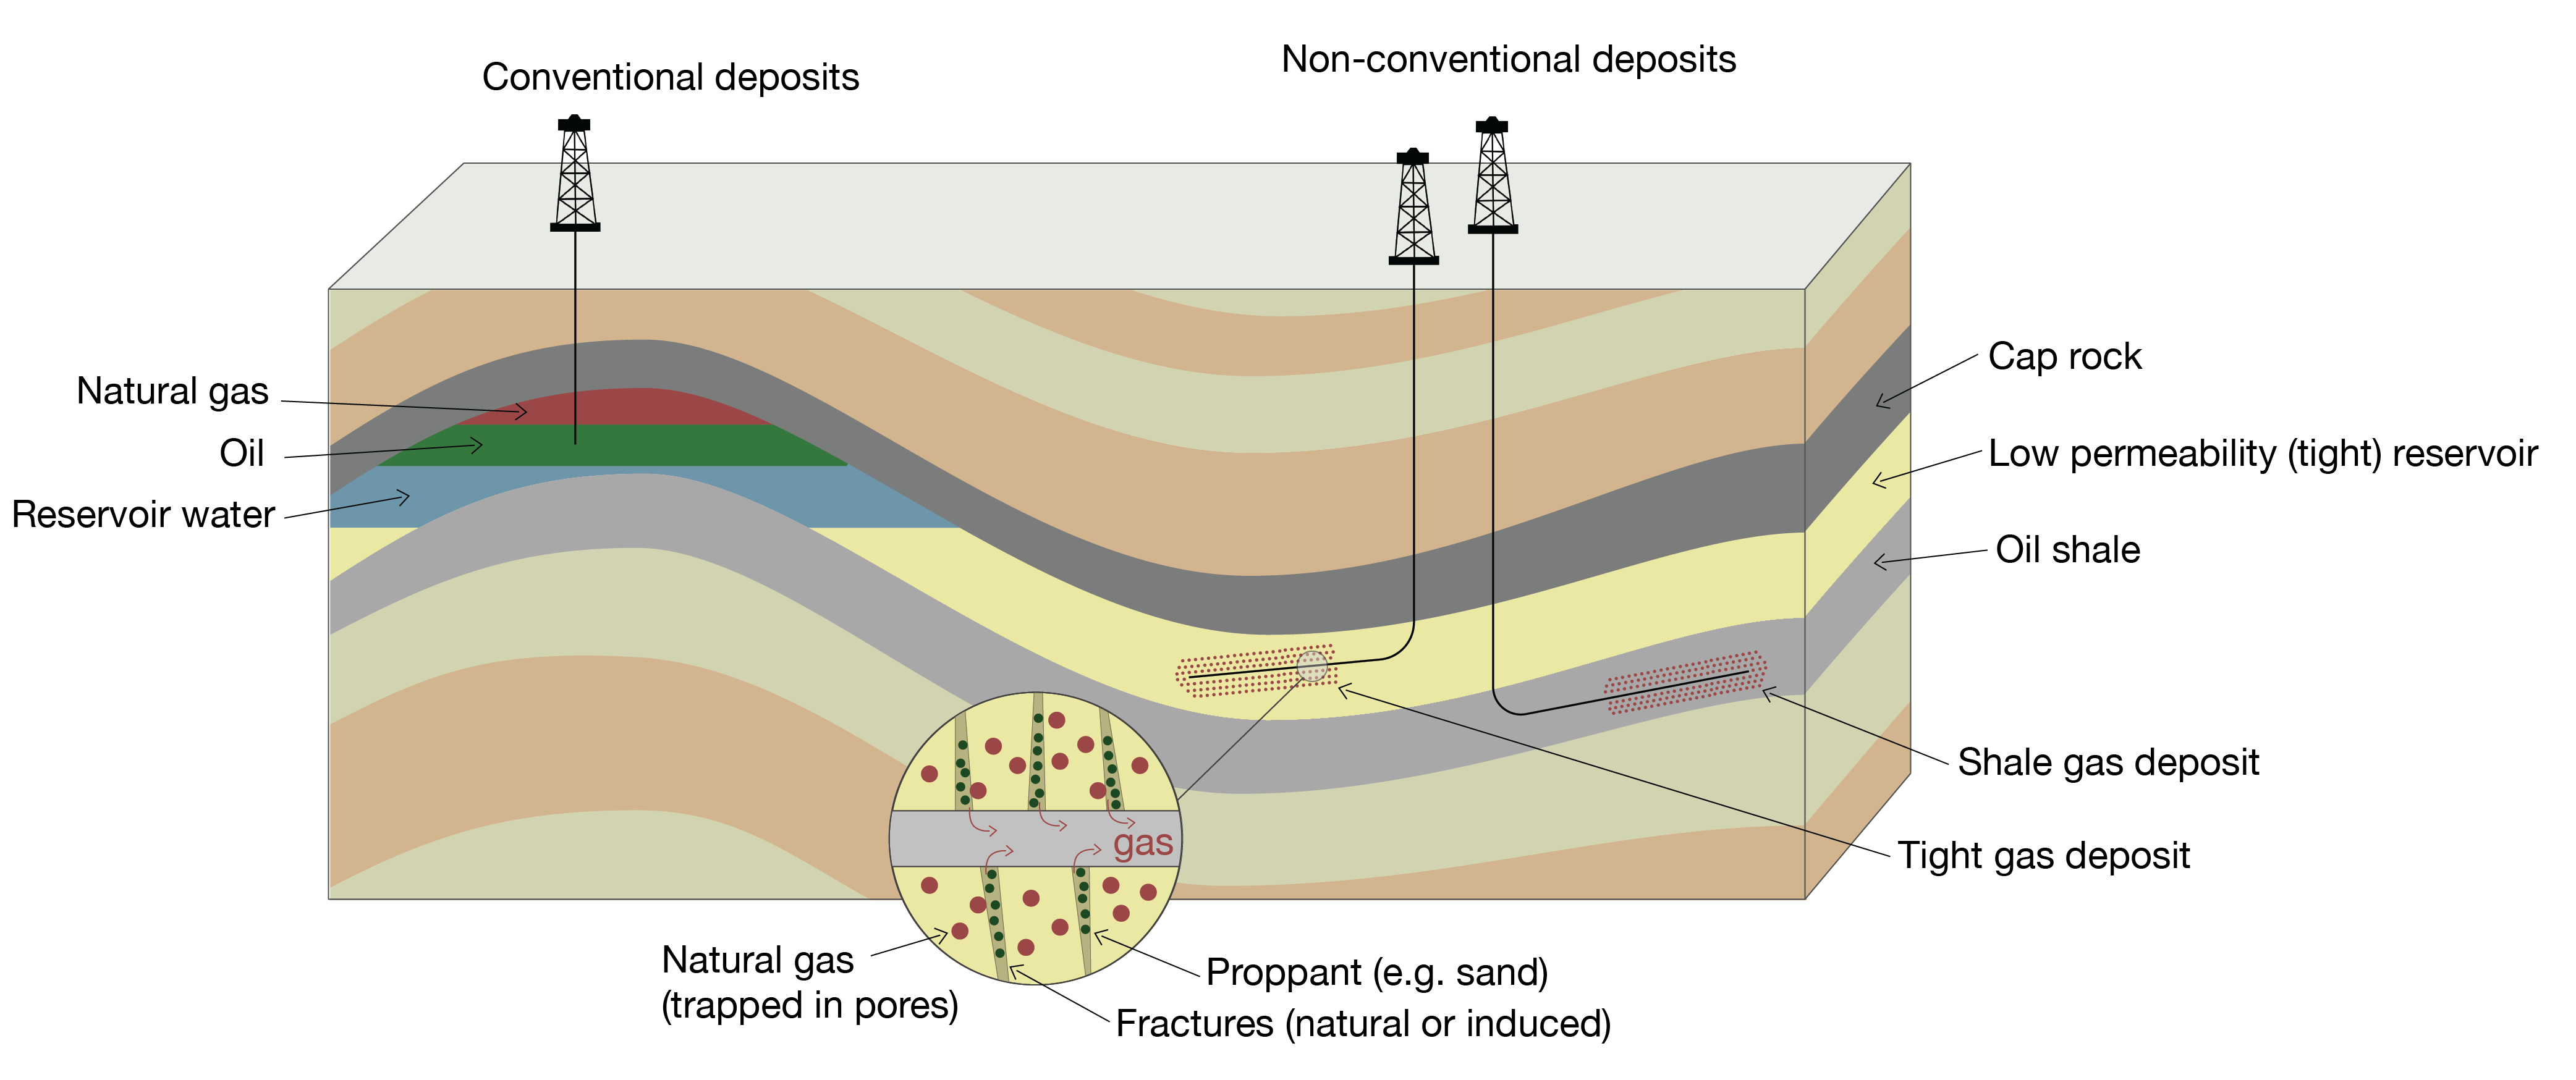
\includegraphics[width=\textwidth]{figures/intro/nonconventional_resources.png}
    \end{center}
\caption{
    Conventional reservoirs contain oil and gas that have migrated upwards
    under pressure until they are trapped by a cap rock (left), while
    non-conventional tight or shale oil and gas reservoirs contain hydrocarbons
    that are trapped in low permeability formations (right).
}
\label{fig:nonconventional_resources}
\end{figure}


To accomplish this task, I propose to use EM geophysical techniques. For EM to be a viable method for imaging the distribution of proppant and fluid within a fractured volume of rock, we require that: (1) the fractured volume of rock have physical properties which are distinct from the background, host rock, (2) the survey must be sensitive to this contrast, and (3) once the data have been collected, they must be interpreted or inverted in a meaningful manner. Note that this is a time-lapse problem; that is, by inducing a fracture, the physical properties of the reservoir have been altered. In order to characterize such a change, we must view the imaging problem as a time-lapse one, and collect data to provide us with a before and an after data-view of the reservoir.

Variations in subsurface electrical conductivity have been used as a diagnostic physical property in sedimentary settings for characterizing geologic formations, and the properties and distribution of fluids within those formations. Hydrocarbons are much more resistive than saline formation fluids. In enhanced oil recovery projects, fluids are injected into the formation, which may be less resistive than the hydrocarbons they replace. These contrasts have been the target of cross-well, surface-to-borehole and borehole-to-surface electromagnetic (EM) methods for reservoir monitoring and characterization applications (cf. \cite{Bevc1991, Wilt1995, marsala2008, marsala2011, Marsala2014}).

In the case of hydraulic fracturing, the physical properties of the fractured volume of the reservoir depend upon the properties of the injected fluid and proppant particles. Saline water may be used, as is often the case when recycled water is used, and electrically conductive proppant may be manufactured and injected \citep{cannan2014electrically, Vengosh2014, King2010}. One or both of these may be used to create a physical property contrast between the host reservoir rock and the fractured volume of the reservoir. This contrast is what we aim to excite using an electromagnetic survey.

Using additives to make a hydraulic fracture a geophysical target is not a new idea. \cite{Byerlee1976} suggested using magnetic particles and a magnetic survey to estimate fracture orientation at distances larger than can be determined by tracers and well logs. To create a fracture with a significant magnetic susceptibility, they suggested using finely crushed magnetite suspended in the fracturing fluid or iron shot, spherical particles of iron which do not crush easily and have a high magnetic susceptibility. They treated the fracture as a plate with a known magnetic susceptibility and collected measurements before and after the fracture operation; measurements of the horizontal magnetic field inside of the injection borehole are used to indicate the orientation of the fracture and surface measurements are used to estimate the fracture geometry. Using an analytic model for the magnetic response of a circular disc in a uniform inducing field, they demonstrated the potential of this technique for simple analog models of two field sites: an engineered geothermal project at Los Alamos, where fractures are induced to circulate fluid through a dry geothermal reservoir and a hydraulic fracture operation for a tight-gas reservoir at Rio Blanco.

Similarly, \cite{Bartel1976} suggest using electrically conductive fracturing fluid and measuring electric potentials at the surface in a direct current (DC) resistivity experiment where one electrode is connected to the injection well and a return electrode is connected to a distant well casing. Potential electrodes are arranged in two concentric rings centered about the injection well with potential differences being measured between electrodes along the same azimuth in the inner and outer rings. Variations in the amplitude of the potential difference with azimuth are used to estimate the orientation of the fracture and to detect asymmetry (e.g. if the fracture extends further one side of the well than the other). Field tests were performed at two sites and demonstrated detectability of fractures in an experiment in the Wattenburg field for fractures at depths of $\sim$2200 m depth. The source electrode was connected to the casing and centered at the depth of the induced fracture (see also \cite{Smith1978}).

Since these initial developments in the late 70's, there have been significant improvements in data quality as well as our ability to model and invert electrical and electromagnetic data in 3D. In conjunction, there have been advancements in fracture operations and imaging techniques such as the use of microseismic, tiltmeters, and pressure-transient analysis to characterize hydraulic fracture. As a result, the questions being asked are more detailed. How complex is the fracture? Is it a simple planar fracture or an extensive network? What is the extent of the propped volume of rock?

To assess if EM can provide insights for helping answer these questions, we need to be able to perform 3D numerical simulations of EM for fractured reservoirs. This prompts a question to be examined in the thesis:
\begin{itemize}
\item{How do we construct a physical property model of a fractured volume of rock that can be used in numerical simulations?}
\end{itemize}

\section{Challenges to electromagnetics with steel-cased boreholes}
\label{sec:challenges-steel-casing}

Hydraulic fracture operations are typically conducted in steel cased wells. These wells presents several significant challenges for modelling and inverting EM geophysical data. Most wells are cased with carbon steel, which has both a large electrical conductivity ($\sim 5.5\times 10^6$ S/m) and magnetic permeability ($> 50 \mu_0$) \citep{wuhabashy1994}. This is a large contrast compared to  typical geologic settings, which typically have conductivities less than 1 S/m and permeabilities similar to that of free space, $\mu_0$. As a result, the casing will have a significant impact on the behavior of the EM fields and fluxes. The properties of the casing, in particular, magnetic permeability, as well as casing thickness, can vary along the length of the well. They also  depend on the quality of the steel and the state of corrosion; this adds another level of complexity to the situation. Well logging tools, such as that described by \cite{brill2012} have been developed to characterize these variations.

Not only does casing introduce a large, variable, physical property contrast, its geometry and scale add to the difficulty. Well casing is cylindrical in shape, typically $\sim$1 cm in thickness, $10-20$ cm in diameter, and may extend several kilometers in depth, while the geologic structures we aim to characterize with the geophysical survey have three dimensional variations in electrical conductivity on the scale of hundreds of meters to kilometers. Approaches tailored to accurately modelling the impact of the casing in simple 1D geologic settings may be geometrically incompatible or computationally prohibitive to use when reservoir-scale, three-dimensional geologic structures and targets are included in the conductivity model.

In much of the early literature, the casing was viewed as a nuisance which distorts the EM signals of interest. Distortion of surface DC resistivity and induced polarization (IP) data, primarily in hydrocarbon settings, was examined in \cite{Wait1983, Holladay1984, Johnston1987} and later extended to grounded source EM and IP in \cite{Wait1985, Williams1985, Johnston1992}. Also in hydrocarbon applications, well-logging in the presence of steel cased boreholes is motivation for examining the behavior of electromagnetic fields and fluxes in the vicinity of casing. Initial work focussed on DC resistivity with \cite{Kaufman1990, Schenkel1990, Kaufman1993, Schenkel1994}, and inductive source frequency domain experiments with \cite{Augustin1989}. \cite{Kaufman1990} derives an analytical solution for the electric field at DC in an experiment where an electrode is positioned along the axis of an infinite-length well. The mathematical solutions presented show how, and under what conditions, horizontal currents leak into the formation outside the well. Moreover, \cite{Kaufman1990} showed, based upon asymptotic analysis, which fields to measure inside the well so that information about the formation resistivity could be obtained. This analysis is extended to include finite-length wells in \cite{Kaufman1993}. \cite{Schenkel1994} show the importance of considering the length of the casing in borehole resistivity measurements, and demonstrate the feasibility of cross-well DC resistivity. They also show that the presence of a steel casing can improve sensitivity to a target adjacent to the well. In frequency domain EM, \cite{Augustin1989} consider a loop-loop experiment, where a large loop is positioned on the surface of the earth and a magnetic field receiver is within the borehole. Magnetic permeability is included in the analysis and a ``casing correction'', effectively a filter due to the casing on inductive-source data, is introduced. This work was built upon for considering cross-well frequency domain EM experiments \citep{Uchida1991, Wilt1996}.

For larger scale geophysical surveys, steel cased wells have been used as ``extended electrodes.'' \cite{Rocroi1985} used a pair of well casings as current electrodes for reservoir characterization in hydrocarbon applications. In near-surface settings \cite{Ramirez1996, Rucker2010, Rucker2012} considered the use of monitoring wells as current and potential electrodes for a DC experiment aimed at imaging nuclear waste beneath a leaking storage tank. Similarly, \cite{Ronczka2015} considers the use of groundwater wells for monitoring a saltwater intrusion and investigates numerical strategies for simulating casings as long electrodes. Imaging hydraulic fractures has been a motivator for a number of studies at DC or EM, among them \cite{Weiss2016, hoversten2017borehole}. Some of these have suggested the use of casings that include resistive gaps so that currents may be injected in a segment of the well and potentials measured across the other gaps along the well \citep{Nekut1995, Zhang2018}.

There has also been an increase in interest in examining the use of electrical or electromagnetic methods deployed on the surface to non-invasively look for flaws or breaks in the casing. \cite{Wilt2018} introduces the idea of using electrical or electromagnetic methods for casing integrity which is further expanded upon in \cite{Wilt2018a}. They show that low-frequency electromagnetic methods are sensitive to variations in wellbore length and demonstrate that their numerical simulations agree with field data collected over two different wellbores at the Containment and Monitoring Institute (CaMI) field site in southern Alberta, Canada. This work provides motivation for further delving into the physics and assessing under which circumstances we can expect to detect a flaw along a wellbore using electrical or electromagnetic methods.

As computing resources increased, our ability to forward-simulate more complex scenarios has improved. However, the large physical property contrasts and disparate length scales introduced when a steel cased well is included in a model still present computational challenges. Even the DC problem, which is relatively computationally light, has posed challenges; those are exacerbated when solving the full Maxwell equations in the frequency (FDEM) or time domain (TDEM) and can become crippling for an inversion. For models where the source and borehole are axisymmetric, cylindrical symmetry may be exploited to reduce the dimensionality, and thus the number of unknowns, in the problem (e.g. \cite{Pardo2013, Heagy2015}).

To reduce computational load in a 3D simulation, a number of authors have employed simplifying assumptions. Several authors replaced the steel-cased well with a solid borehole, either with the same conductivity as the hollow-cased well (e.g. \cite{Um2015, Puzyrev2017}) or preserving the cross sectional conductance (e.g. \cite{Swidinsky2013, Kohnke2017}), so that a coarser discretization may be used; \cite{Haber2016} similarly replaces the borehole with a coarser conductivity structure and adopts an OcTree discretization to locally refine the mesh around the casing. \cite{Yang2016} uses a circuit model and introduces circuit components to account for the steel cased well in a 3D DC resistivity experiment. Also for DC resistivity, \cite{Weiss2017} develops a hierarchical finite element approach in which conductivity values can be defined on edges, facets, and volumes on the mesh. In doing so, multiple thin boreholes, which may be deviated or horizontal, can be accurately modelled in a DC experiment. Another approach has been to replace the well with an ``equivalent source'', for example, a collection of representative dipoles, inspired from \cite{cuevas2014}, or with linear charge distributions for a DC problem \citep{Weiss2016}. For the frequency domain electromagnetic problem, a method of moments approach, which replaces the casing with a series of current dipoles, has been taken in \cite{Kohnke2017}.

For 3D survey geometries, only a handful of forward simulations which explicitly discretize the casing have been demonstrated, and they have been achieved at significant computational cost. Recent examples, including \cite{Commer2015, Um2015, Puzyrev2017}, perform time and frequency domain simulations with finely-discretized boreholes; they required the equivalent of days of compute-time for a single forward simulation to complete. While these codes will undoubtedly see improvements in efficiency, there remains a need to accurately discretize the casing at modest computational cost both to serve as tool which these codes can compare against as well as a need for researchers to be able to interact with and explore the behavior of the currents, charges, electric and magnetic fields and fluxes to develop an understanding of the physics in these high-contrast settings.

There are a host of research questions to be explored in the context of highly conductive, permeable, steel cased wells in electromagnetic applications. This thesis is concerned with developing an understanding of the physics of electromagnetics in settings with steel cased wells. In order to delve into the physics, we must have a mechanism for simulating Maxwell's equations which raises the question:
\begin{itemize}
\item{How do we develop a numerical approach that allows us to sufficiently discretize the steel casing so that we can not only simulate DC and EM data, but also explore the finer details of the currents, charges, electric and magnetic fields?}
\end{itemize}

Assuming a numerical strategy can be developed, we can then begin to explore questions about the physics. At the DC limit,
\begin{itemize}
\item{How do the currents, charges and electric fields behave in settings with steel cased wells? What are the implications for survey design?}
\item{Are there physical insights which, when incorporated into numerical algorithms, reduce the computational cost of simulations with steel-cased wells?}
\end{itemize}

Finally, electromagnetic experiments introduce the complication of time-variation in the fields and fluxes as well as the additional concern of variable magnetic permeability in the model. Though the influence of the magnetic permeability of steel-casings has been explored for inductive source EM (e.g. where the source is a circular loop or magnetic dipole) \citep{wuhabashy1994}, the influence of magnetic permeability on grounded-source EM surveys (e.g. where two electrodes are used to inject current into the earth, similar to a DC resistivity experiment) is relatively unexplored. This prompts questions like:
\begin{itemize}
\item{How do the fields and fluxes behave in an EM experiment which includes a steel-cased well?}
\item{What impact does magnetic permeability have on the behavior of the fields and fluxes? How important is it to consider in numerical simulations?}
\end{itemize}

These questions will serve as motivation for three chapters on steel-cased wells in the thesis.

\section{Research motivation and thesis structure}
The common theme throughout the thesis is the motivation to image subsurface injections -- specifically proppant and fluid injected during a hydraulic fracturing operation. To this end, I consider three main topics that comprise five chapters in the thesis:
\begin{itemize}
    \item{Building a physical property model for a fractured volume of rock (Chapter \ref{ch:phys-prop-model})}
    \item{Developing a physical understanding of electrical and electromagnetic methods when steel-cased wells are present (Chapter \ref{ch:casing-software}, \ref{ch:casing-dc}, and \ref{ch:casing-em})}
    \item{Formulating and solving the inverse problem for a fractured volume of rock (Chapter \ref{ch:inversion})}
\end{itemize}
Each of these topics is discussed in further detail below.

The research chapters in this thesis make use of fundamental knowledge that needs to be presented. Rather than insert that introductory material into the individual chapters, they are included at the end of this chapter. The background elements pertain to:
\begin{itemize}
\item{Electromagnetic geophysics: introducing Maxwell's equations and EM geophysical surveys}
\item{Geophysical inversions: formulating the inverse problem}
\end{itemize}
These are successively presented in Sections \ref{sec:background-em} and \ref{sec:background-inversions} after I have introduced the research material in this thesis.

\subsection{Homogenization strategy for hydraulic fractures}

Chapter \ref{ch:phys-prop-model} develops a strategy for estimating a bulk conductivity of a fractured volume of rock.  I break the problem into two steps, first estimating the effective conductivity of a mixture of electrically conductive proppant and fluid and second, estimating the conductivity of a fractured volume of rock where the fractures are filled with the proppant-fluid mixture. Having constructed a physical property model for a modest-sized fracture operation, I then demonstrate feasibility of detecting EM signal sensitive to the fracture using a well-established cross-well EM survey. At this stage, I neglect the influence of steel-cased wells. The aim of this chapter is to provide a reasonable estimate for the conductivity of a fractured volume of rock; future lab studies may provide an improved relationship between the conductivity of the proppant, fluid, host rock and their relative concentrations.

The homogenization strategy taken in this chapter is based on established methods in effective medium theory \citep{Bruggeman1935} which have previously been considered for fractured rocks \citep{Berryman2013}. The main contributions of this chapter are: algorithmic improvements to the effective conductivity calculation presented by \cite{Berryman2013}, and the discussion of the two-stage workflow which allows various proppant-fluid mixtures to be considered (e.g. a fully conductive proppant-pack, mixture of standard sand or ceramic proppant and conductive proppant).


\subsection{Steel casings}

The intention in this thesis is to advance our understanding of the physics of EM in settings with steel-cased wells. This understanding can then be used to develop appropriate approximations in order to reduce computational cost, and to help calibrate our expectations of the results of more advanced numerical techniques. To this end, I consider three topics, each corresponding to one chapter in the thesis, to advancing our physical understanding. This thesis does not contend with the challenge of efficiently simulating the DC or EM equations for settings with deviated or horizontal wells, nor do I consider settings with multiple wells or surface infrastructure. In a field survey, these complexities will need to be considered.

Chapters \ref{ch:casing-software}, \ref{ch:casing-dc}, and \ref{ch:casing-em} contend with some of the challenges of performing DC and EM surveys in settings with steel-cased wells. In Chapter \ref{ch:casing-software}, I present a mimetic finite volume implementation for simulating Maxwell's equations at DC, in frequency and in time, on cylindrically symmetric and 3D cylindrical meshes (which include an azimuthal discretization). Although cylindrically symmetric meshes are common in EM modelling, cylindrical meshes which include an azimuthal discretization are not. A cylindrical mesh conforms to the geometry of a vertical borehole and thus, can greatly reduce the size of the mesh, and resultant cost of the computation, while still allowing for significant refinement in the vicinity of the borehole. The purpose of this implementation is to facilitate investigation into the physical behavior of EM fields and fluxes in this high-contrast setting. I consider two forms of validation: numerical validation and validation of the physical behavior. For numerical validation, I compare results of a forward simulation with independently developed codes \citep{Haber2007, Commer2015, Yang2016}. For validation of the physical behavior, I compare features of the simulated currents, charges, and electric fields to the behavior expected from the asymptotic analysis in \cite{Kaufman1990, Kaufman1993} at DC, and similarly, compare the behavior of the magnetic fields and fluxes in the presence of conductive and permeable pipes with the lab studies and analytical work contained in \cite{Augustin1989} for inductive source frequency-domain electromagnetics.

Chapter \ref{ch:casing-dc} focuses on developing an understanding of the physics of casings in a DC resistivity experiment. I start by considering the related application of casing integrity. In a casing integrity experiment, the aim is to detect a flaw or break in the casing which might be due to corrosion or failure under mechanical stresses. Wellbore integrity surveys are typically conducted with wireline tools, but more recently, \cite{Wilt2018} introduced the idea of conducting a survey from the surface. This application provides the opportunity to build a physical understanding about the behavior of the currents, charges, and electric fields in a DC experiment with casing. I investigate factors that influence the feasibility of detecting a flaw, including the conductivity of the background and casing, depth to the flaw, and impact on the signal if the whole circumference or only a portion of the circumference of the casing is compromised. I also consider the location of the return electrode and its impact on the measured data. Many of the concepts developed in this section inform survey design elements in the next section, which considers DC resistivity survey for a conductive or resistive target adjacent to the well. I look at survey design elements, including the impact of the source electrode location on the resultant currents over the depth-interval of interest, and consider the impact of parameters such as the conductivity of the target and whether the target is electrically connected to the casing or not. The final topic in this chapter considers approximations to the steel-cased well in order to reduce the computational cost of the forward model. There is discrepancy among current literature as to whether the contrast between the background and the casing is the important quantity to conserve (e.g. \cite{Um2015}) or if the product of the conductivity and the cross-sectional area of the casing should be preserved (e.g. \cite{Swidinsky2013}). I compare both approaches to resolve this question, demonstrate that the product of the cross-sectional area of the casing and its conductivity is the important quantity to preserve in DC resistivity experiments, and discuss implications of choosing an incorrect approximation.

Chapter \ref{ch:casing-em} explores important aspects of electromagnetics in settings with steel cased well. I begin by demonstrating the behavior of currents through time in time-domain EM simulation with a conductive well. The geometry of the currents through time is rather complex, even in this seemingly simple experiment. Building from this, I then consider magnetic permeability and demonstrate how permeability alters the behavior of the currents and in turn, discuss the impact permeability can have on data measured at the surface. Finally, I revisit approaches for approximating steel cased wells developed at DC and explore some of the subtleties that arise in EM experiments.

\subsection{Inversions for subsurface injections}
Chapter \ref{ch:inversion} returns to the application of hydraulic fracturing and examines the inverse problem for a fractured volume of rock. Using a DC resistivity experiment, I explore both voxel-based and parametric strategies for extracting information about the fractured volume of rock. These inversions demonstrate some of the challenges caused by steel cased wells and their influence on the sensitivity. Finally, I show how effective medium theory can be incorporated into the inversion and frame the inverse problem as an inversion for fracture concentration. This alters the sensitivity and provides the opportunity to incorporate a constraint on the volume of injected proppant and fluid.

\subsection{Appendices}
The thesis additionally includes 5 Appendices. Appendix \ref{app:code_list} provides a listing of the source code used to perform all of the examples shown in the thesis. Following this, there are two technical appendices, Appendix \ref{app:concentric_spheres} and \ref{app:scemt-derivs}, which support content in Chapters \ref{ch:phys-prop-model} and \ref{ch:inversion}, respectively. Appendix \ref{app:simpegem} describes the open-source software used in this thesis to simulate and invert Maxwell's equations. The final appendix, Appendix \ref{app:education}, discusses how the open-source software development practices adopted in this thesis and the broader SimPEG community are similarly used for the development of interactive educational resources for geophysics in the GeoSci.xyz project (\href{https://geosci.xyz}{https://geosci.xyz}).


\subsection{A note on reproducibility and dissemination}

Although simulating and inverting data in settings with steel-cased wells has practical applications, within the realm of geophysics, and even within EM geophysics, it is a narrow topic. The value in focussing on specific applications is that each application has its own subtleties and tangible details that must be worked through. In their own right, the discoveries that are made by working through these details are of value to the application-at-hand. However, this does not have to be the limit of their impact. If you choose to take the perspective that the problem-at-hand is an instance of a larger class of research questions, this allows you to view the methods and software needed to make incremental scientific discoveries as reusable components. It is then worth the investment of effort to develop and refactor these pieces so that they are modular building blocks that fit into a larger framework and are of use to a broader community. This is the perspective I have sought to take as I conducted the research described in this thesis.

The simulations and inversions build on and contribute to the SimPEG framework, which is described in \cite{Cockett2015, Heagy2017, Cockett2017}. SimPEG is written in python and is open-source, licensed under the permissive MIT license. Source code for all of the examples shown are also openly licensed and are available on GitHub as a combination of python scripts and Jupyter notebooks. Each chapter has a corresponding code-repository; Appendix \ref{app:code_list} provides a summary of where these can be accessed. My intention in providing all of the source-code is to be transparent about the work completed; in addition, I hope these developments are of use and value to the broader geophysics community.
\section{Background: Electromagnetic geophysics}
\label{sec:background-em}
Before moving into the research content of the thesis, I will provide a brief overview of the governing equations in electromagnetics and recommend \cite{Ward1988} and \cite{emgeosci} for more in-depth discussion on the physics. For an overview of how to numerically solve Maxwell's equations, I refer the reader to \cite{Haber2014}.
\subsection{Governing equations}
The equations which govern the physics of EM are Maxwell's equations:
\begin{equation}
\begin{split}
    \nabla \times \vec{e} + \frac{\partial \vec{b}}{\partial t} &= 0 \\
    \nabla \times \vec{h} - \frac{\partial \vec{d}}{\partial t} &= \vec{j}
\end{split}
\label{eq:maxwell_time_full}
\end{equation}

where $\vec{e}$ is the electric field (V/m), $\vec{b}$ is the magnetic flux density (T), $\vec{h}$ is the magnetic field (A/m), $\vec{d}$ is the electric displacement (C/m$^2$), $\vec{j}$ is the current density (A/m$^2$). The first equation is Faraday's law; it describes how a time-varying magnetic flux generates rotational electric fields. The second equation is the Ampere-Maxwell equation (Maxwell's contribution was the addition of the displacement current term, $\partial \vec{d} / \partial t$). It describes how currents generate rotating magnetic fields.

It is sometimes also convenient to consider Maxwell's equations in the frequency domain. Following \cite{Ward1988}, I use the $e^{i\omega t}$ Fourier transform convention, namely,
\begin{equation}
\begin{split}
    F(\omega) &= \int_{-\infty}^{\infty} f(t) e^{-i\omega t} dt \\
    f(t) &= \int_{-\infty}^{\infty} F(\omega) e^{-i\omega t} d\omega
\end{split}
\label{eq:fourier-transform}
\end{equation}

where capital letters denote functions expressed in the frequency domain and lowercase letters denote functions expressed in the time-domain.
In the frequency domain, Maxwell's equations are given by
\begin{equation}
\begin{split}
    \nabla \times \vec{E} + i \omega\vec{B} &= 0 \\
    \nabla \times \vec{H} - i \omega\vec{D} &= \vec{J}
\end{split}
\label{eq:maxwell_freq_full}
\end{equation}


These partial differential equations are coupled through the constitutive relations which relate the fields and fluxes through physical properties:
\begin{equation}
\begin{split}
\vec{J} &= \sigma \vec{E} \\
\vec{B} &= \mu \vec{H} \\
\vec{D} &= \varepsilon \vec{E}
\end{split}
\label{eq:constitutive_relations_full}
\end{equation}

where $\sigma$ is electrical conductivity (S/m), $\mu$ is magnetic permeability (H/m), and $\varepsilon$ is the dielectric permittivity (F/m). Electrical conductivity varies over many orders of magnitude; two examples on the extreme ends are the conductivity of air, $\sim10^{-8}$ S/m, and the conductivity of steel, $\sim 10^6$ S/m. The reciprocal of electrical conductivity is resistivity ($\rho = 1/\sigma$), which has units of $\Omega$m. Throughout the thesis, resistivity and conductivity will be used interchangeably. The value of magnetic permeability is often taken to be that of free-space, $\mu_0 = 4\pi\times10^{-7}$ H/m, in geophysical electromagnetic applications, as the permeability of most earth-materials ranges from 1-10 $\mu_0$ \citep{Telford1990}. The permeability of steel, however, is $\sim 100 \mu_0$; thus, for settings with steel-cased wells the simplifying assumption that $\mu=\mu_0$ cannot necessarily be justified. The value of dielectric permittivity varies between the free-space value of $\varepsilon_0=8.85\times10^{-12}$ F/m and the dielectric permittivity of water, $80\varepsilon_0$ \citep{Telford1990}. Variations in dielectric permittivity are relevant at high frequencies, such as those used in ground penetrating radar (GPR) surveys ($> 10^5$ Hz), but in most geophysical electromagnetic surveys, late-time or low frequencies are employed as the high-frequency signals attenuate rapidly in conductive earth-materials. As such, the quasi-static approximation, which neglects displacement currents (the $\partial \vec{d} / \partial t$-term in equation \ref{eq:maxwell_time_full} and the $i\omega\vec{D}$ term in equation \ref{eq:maxwell_freq_full}), is commonly adopted, and will be used throughout the thesis. Under the quasi-static assumption, Maxwell's equations are given by:
\begin{equation}
\begin{split}
    \nabla \times \vec{e} &= -\frac{\partial \vec{b}}{\partial t} \\
    \nabla \times \vec{h}  &= \vec{j}
\end{split}
\label{eq:maxwell_time_quasi}
\end{equation}

in time, and:
\begin{equation}
\begin{split}
    \nabla \times \vec{E} &= -i \omega\vec{B}  \\
    \nabla \times \vec{H} &= \vec{J}
\end{split}
\label{eq:maxwell_freq_quasi}
\end{equation}

 in frequency.

In the electrostatic limit, the time-derivative terms vanish. Taking the divergence of Ampere's law, and recognizing that the electric field $\vec{e}$ is curl-free and can therefore be expressed as the gradient of a scalar potential $\phi$, gives us the governing equations for the DC resistivity problem:
\begin{equation}
\begin{split}
\nabla \cdot \vec{j} &= I\left(\delta(\vec{r} - \vec{r}_{s^{+}}) - \delta(\vec{r} - \vec{r}_{s^{-}})\right) \\
\vec{e} &= - \nabla \phi
\end{split}
\label{eq:dc_equations}
\end{equation}

Here $\vec{j}$ is the current density, $I$ is the magnitude of the source current, and $\vec{r}_{s^+}$ and $\vec{r}_{s^-}$ are the location of the positive and negative source electrodes, respectively. The electric field and the current density are related through Ohm's law (the first equation in equation \ref{eq:constitutive_relations_full}), which we can invoke to reduce the two first-order partial differential equations in equation \ref{eq:dc_equations} to a single, second order equation in $\phi$:
\begin{equation}
\nabla \cdot \sigma \nabla \phi = - I\left(\delta(\vec{r} - \vec{r}_{s^{+}}) - \delta(\vec{r} - \vec{r}_{s^{-}})\right)
\label{eq:dc_equation_second_order}
\end{equation}

This Poisson equation can be solved for the electric potential, $\phi$, from which values of the currents and electric fields can be directly computed. In addition to considering the current density and electric fields, I will also present results in terms of charges throughout the thesis. The charge density is related to the electric field through
\begin{equation}
\nabla \cdot \vec{e} = \frac{\rho_f}{\varepsilon_0}
\label{eq:charge_density}
\end{equation}


\subsection{Geophysical surveys}
To generate data, we require that a source be used to excite a response and that receivers measure the resultant fields and/or fluxes. Sources can be natural, plane-wave sources, as in the case of the magnetotelluric method, or they can be controlled, man-made sources. Broadly speaking, two categories of controlled sources exist: inductive sources and grounded sources. Inductive sources consist of a loop of wire through which a time-varying current is passed, this in turn generates time-varying magnetic fields which act as the source fields, as shown in an airborne EM example in Figure \ref{fig:inductive-sources}. The time-varying magnetic field created by these systems induces currents in the conductive earth which, in turn, create secondary magnetic fields which can be measured at or above the surface. Within reservoir settings, cross-well EM is a commonly applied inductive source survey \citep{Wilt1995}.


\begin{figure}
    \begin{center}
    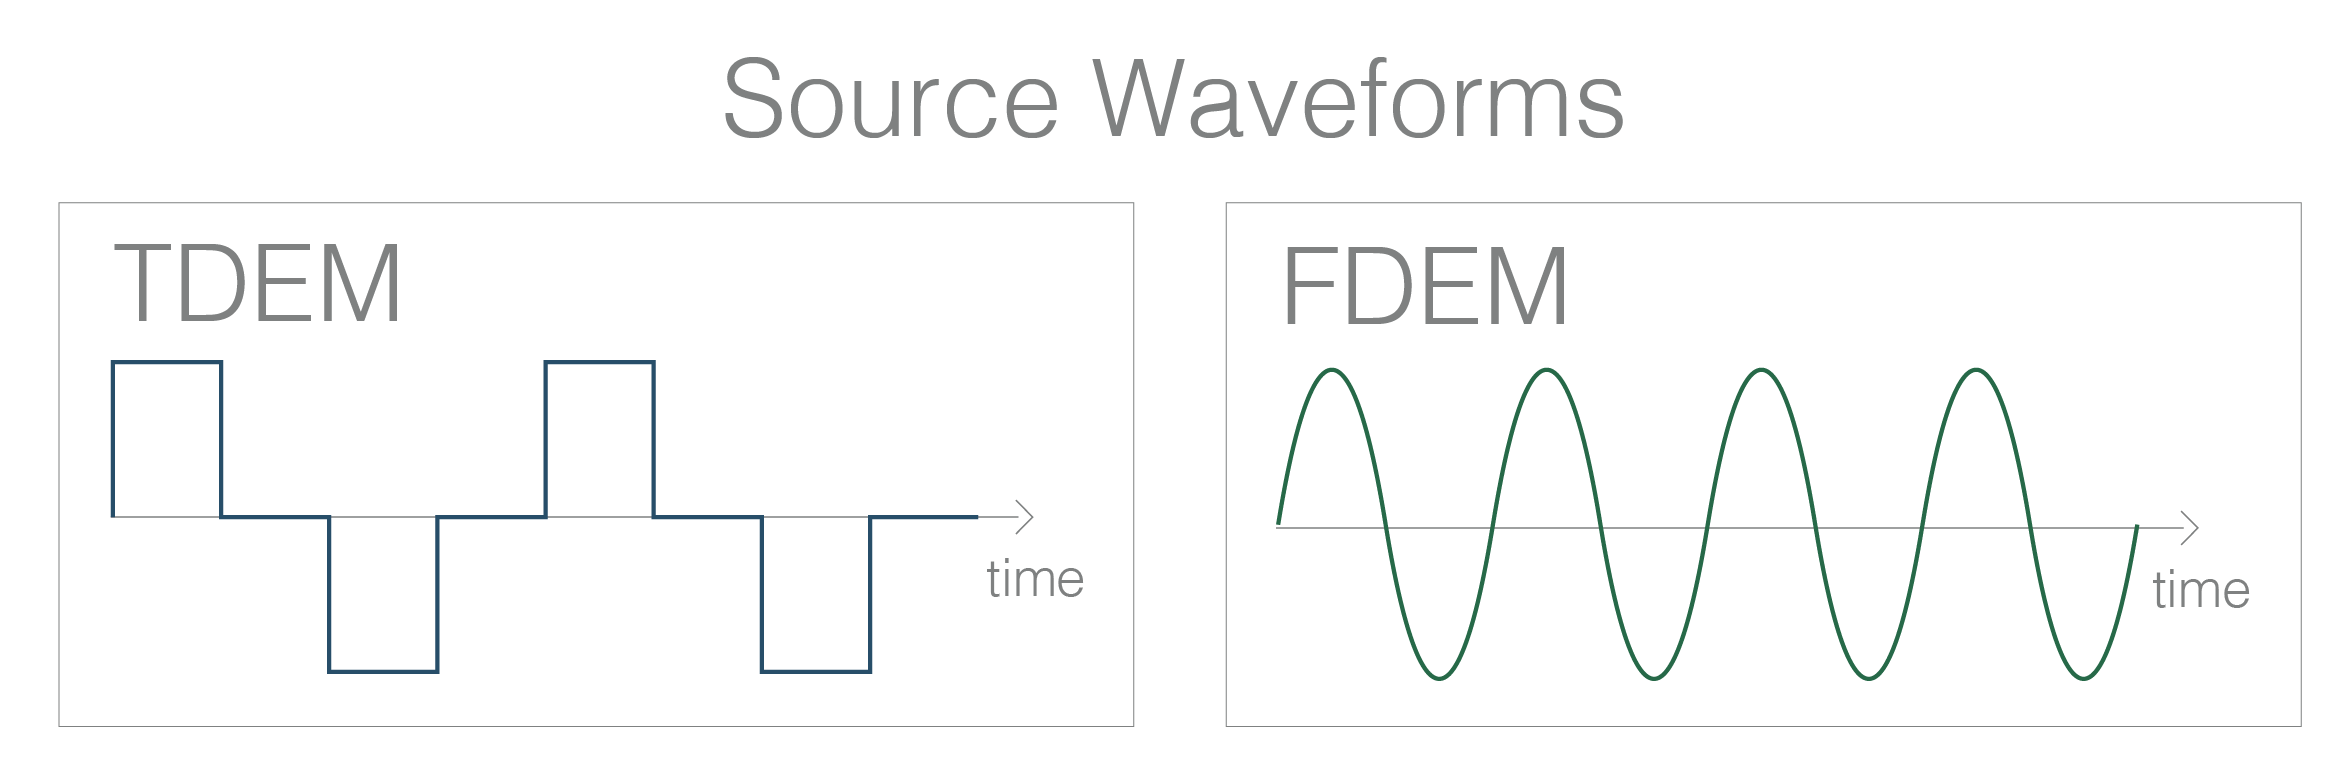
\includegraphics[width=0.7\textwidth]{figures/intro/waveforms.png}
    \end{center}
\caption{
    The choice of whether to solve the EM equations in the time-domain (TDEM) or the frequency domain (FDEM) depends upon the transmitter waveform; a step-off-type waveform (left) lends itself to a solution approach in the time domain and a harmonic signal (right) is typically addressed in the frequency domain.
}
\label{fig:waveforms}
\end{figure}



\begin{figure}
    \begin{center}
    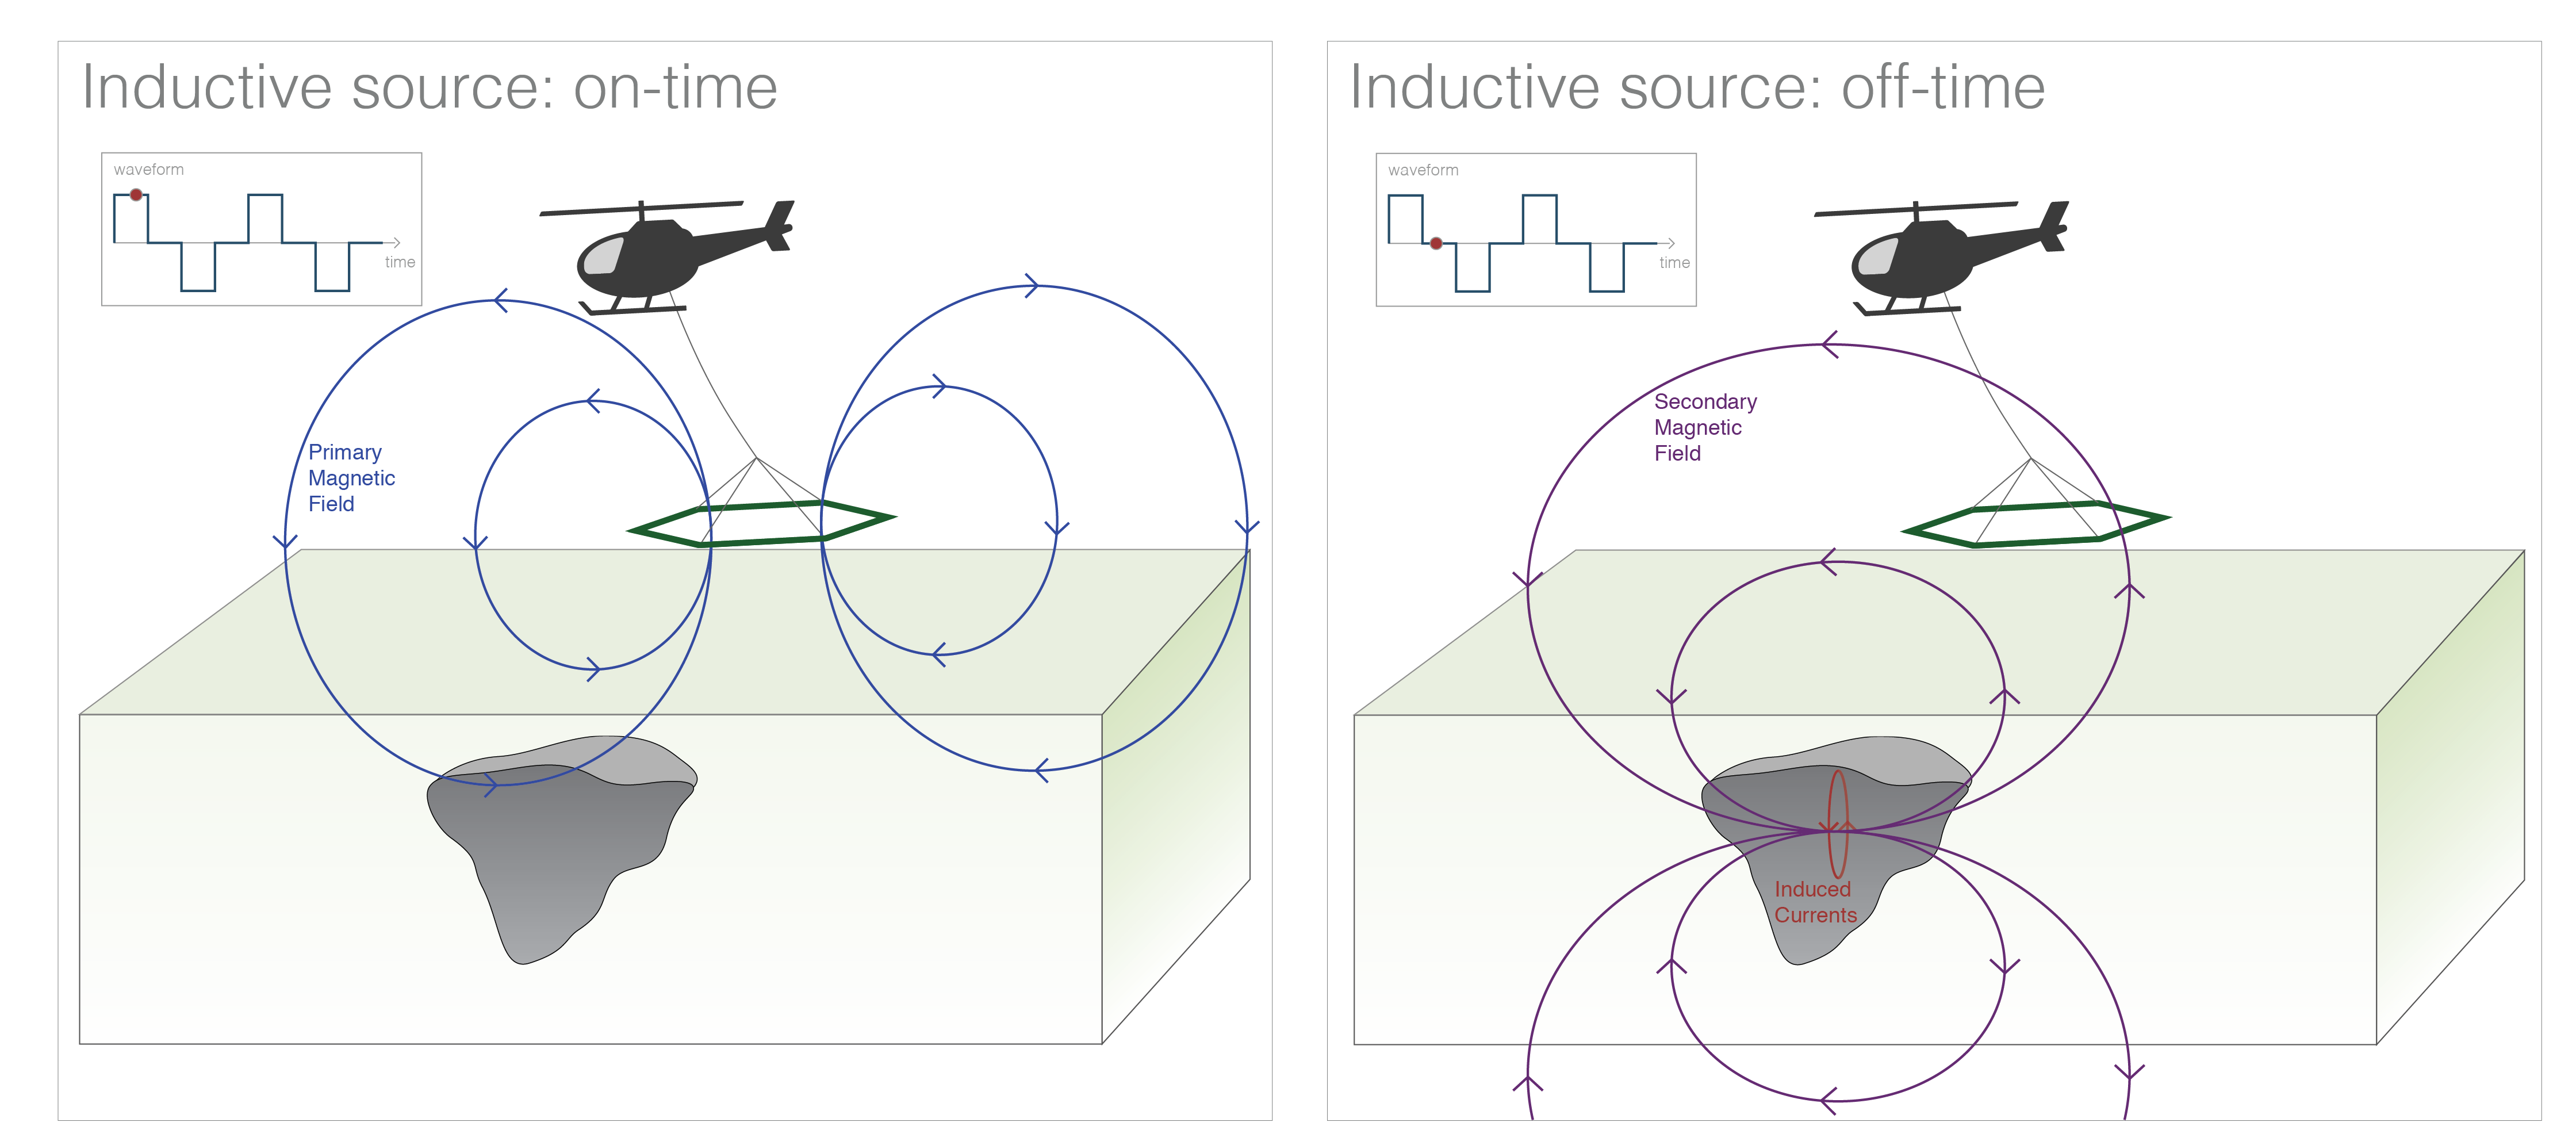
\includegraphics[width=\textwidth]{figures/intro/inductive-sources.png}
    \end{center}
\caption{
    Time-domain inductive source experiment. (Left) a steady-state current is passed through the transmitter loop, generating a primary magnetic field. (Right) This current is shut-off, causing a change in magnetic flux. The changing magnetic flux induces secondary currents in conductors, which in turn create secondary magnetic fields that can be measured at receivers above, on, or within the earth.
}
\label{fig:inductive-sources}
\end{figure}


Grounded sources require an electrical connection between the source and the earth. Two electrodes are positioned on, or in, the ground, the positive electrode injects current and a return electrode is a current-sink, as shown in Figure \ref{fig:grounded-sources}. In the electrostatic limit, a grounded-source experiment is simply a DC resistivity experiment. Galvanic currents flow through the earth and cause charges to build up at conductivity interfaces, generating electric potentials which can be measured at the surface or within boreholes. Electromagnetics introduces a time-varying component. The time-varying current flowing through the wire generates a time-varying primary magnetic field. This induces vortex currents in conductive structures within the earth. Receivers can measure electric fields, magnetic flux, or time-variations in the magnetic flux or some combination of these.

\begin{figure}
    \begin{center}
    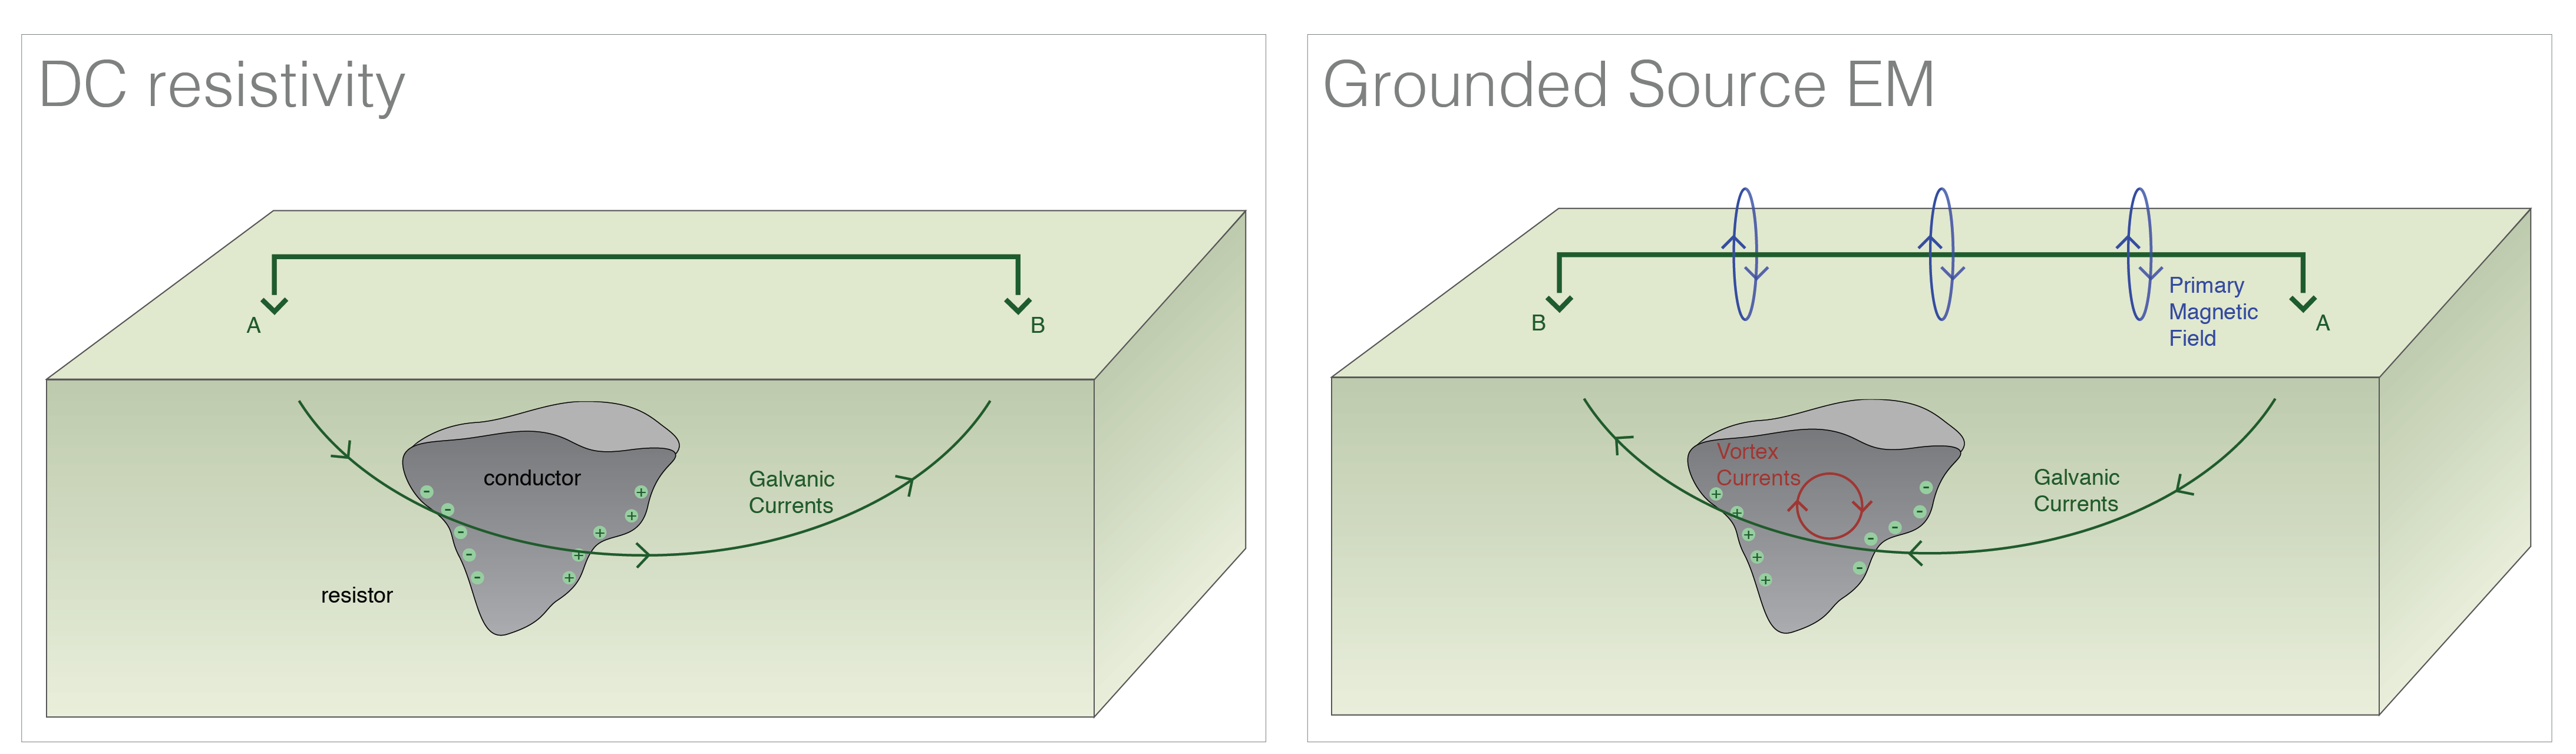
\includegraphics[width=\textwidth]{figures/intro/grounded-sources.png}
    \end{center}
\caption{
    (Left) Direct current resistivity experiment in which a steady-state current is injected into the earth, and
    (Right) a grounded source electromagnetic experiment which uses a time-varying source current.
}
\label{fig:grounded-sources}
\end{figure}


Two things are needed to generate data that are sensitive to a target or structure of interest. First, the source must be capable of getting EM energy to the target to excite a response, and second, the response must reach the receivers with sufficient amplitude to be measurable. A measurable signal is one which is (a) above the noise floor of the receivers, and (b) comprises a significant percentage of the primary (that is, the response with no target present). Numerical simulation of Maxwell's equations is a critical component for assessing feasibility of detecting a target, and is an essential element of the inverse problem in which we aim to estimate a model from measured data. Within the thesis, I discuss the machinery used to perform numerical simulations in Chapter \ref{ch:casing-software} and in Appendix \ref{app:simpegem}.
\section{Background: Geophysical Inversions}
\label{sec:background-inversions}

Once data have been collected, an inverse problem can be formulated. The goal of the inversion is to extract information about the subsurface from the data. Formulating, implementing and solving the inverse problem can be viewed as a workflow consisting of inputs, implementation, and evaluation, as shown in Figure \ref{fig:inversion_workflow_bullets}. The inputs are composed of the data, the governing equations, and prior knowledge or assumptions about the setting. In the case of the fracturing problem, this may include well-log resistivity measurements which provide information about the background, knowledge of where the fracture was initiated, and the volumes of proppant and fluid pumped to create the fracture.
The implementation consists of two broad categories: the forward simulation and the inversion. The forward simulation is the means by which we solve the governing equations given a model, and the inversion components evaluate and update this model. I consider a gradient based approach, which updates the model through an optimization routine. The output of this implementation is a model, which, prior to interpretation, must be evaluated. This requires considering, and often re-assessing, the choices and assumptions made in both the input and implementation stages (c.f. \cite{Oldenburg2005, Haber2014a, Cockett2015}).

\begin{figure}
    \begin{center}
    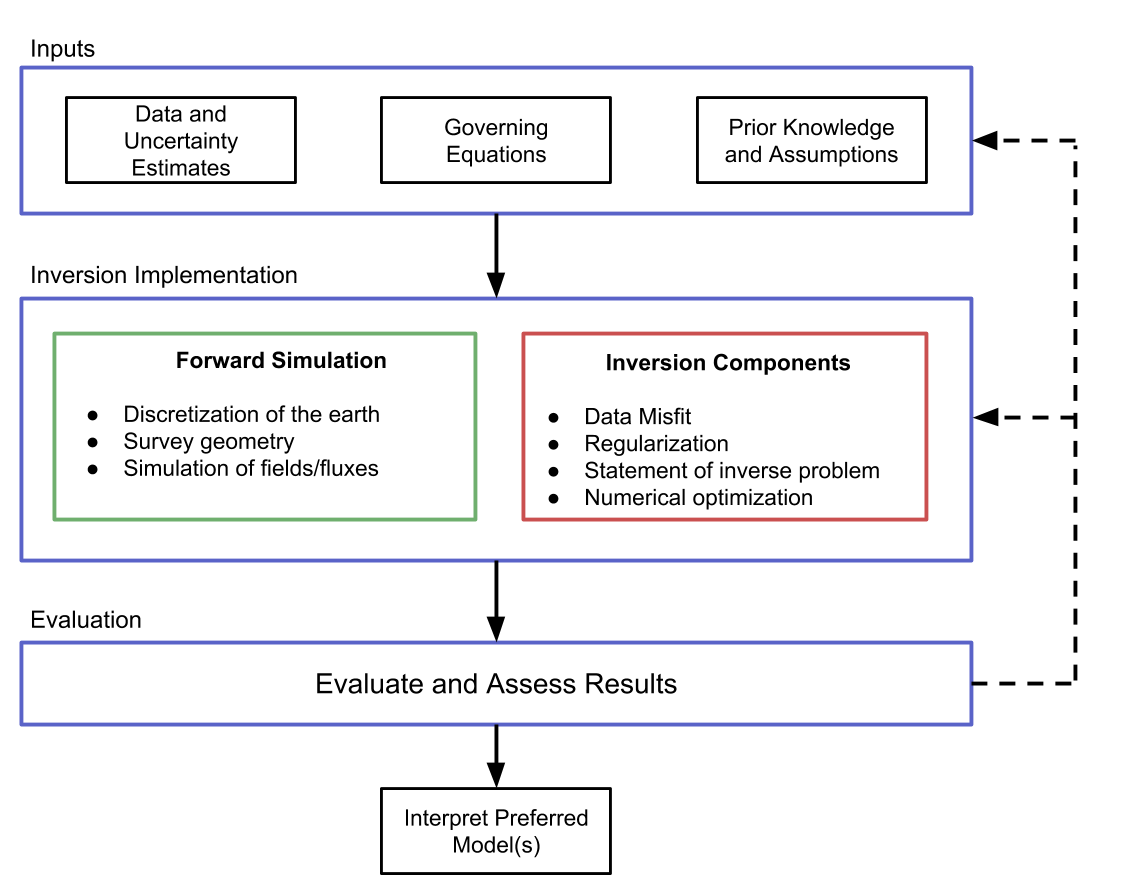
\includegraphics[width=\textwidth]{figures/intro/inversion_workflow_bullets.png}
    \end{center}
\caption{
    Overview of a geophysical inversion workflow. Adapted from \cite{Cockett2015}.
}
\label{fig:inversion_workflow_bullets}
\end{figure}


\subsection{Formulating and solving the inverse problem}
In this section, I provide a brief overview of geophysical inversions, adapted from \cite{Cockett2015}; for more detail and examples, the reader is referred to \cite{Oldenburg2005, Cockett2015} as well as Appendix \ref{app:simpegem} for details specific to forward and inverse modelling in electromagnetics.

The aim of a geophysical inversion is to use the collected data to extract information about the subsurface. In a given survey, a datum can be written as
\begin{equation}
F_i[\mathbf{m}] + \epsilon_i = d_i
\label{eq:geophysical_datum}
\end{equation}

where $F[\cdot]$ is the forward simulation operator; for an electromagnetic problem, it simulates Maxwell's equations given a source and samples the relevant fields and fluxes at the receiver locations. The physical properties of the subsurface are captured by the variable $\mathbf{m}$, which I refer to as the inversion model. The noise is described by $\epsilon_i$, and $d_i$ is the observed datum. A survey usually includes multiple sources and receivers, resulting in the observed data $\mathbf{d}_{\rm obs} = [d_1, ... , d_N]$ and some estimate of their uncertainties -- often assumed to be Gaussian. If the noise is Gaussian, then an appropriate measure of the data misfit is the $l_2$-norm of the difference between the predicted data obtained through a forward simulation and the observed data, namely
\begin{equation}
\phi_{\rm d}(\mathbf{m}) = \frac{1}{2}\|\mathbf{W}_{\rm d}(F[\mathbf{m}] - \mathbf{d}_{\rm obs})\|^2
\label{eq:data_misfit}
\end{equation}

$\mathbf{W}_{\rm d}$ is a diagonal matrix whose elements are equal to $\mathbf{W}_{\rm d_{ii}}=1/\epsilon_i$ where $\epsilon_i$ is an estimated standard deviation of the $i$\textsuperscript{th} datum. Ideally, the noise model should also capture deficiencies in the ability of the forward simulation to accurately describe the physics. A common choice in geophysical inversions is to assign a $\epsilon_i = floor + \%|d_i|$.
Percentages are generally required when there is a large dynamic range of the data. A percentage alone can cause great difficulty for the inversion if a particular datum acquires a value close to zero, and therefore we include a floor.

In addition to a metric that evaluates the size of the misfit, it is also required that we have a tolerance, $\phi_d^*$; models satisfying $\phi_d(\mathbf{m}) \leq \phi_d^*$ are considered to adequately fit the data \citep{Parker1994}. If the data errors are Gaussian and we have assigned the correct standard deviations, then the expected value of $\phi_d^* \sim N/2$, where $N$ is the number of data. Note that the division by 2 is because the statement of the data misfit includes the factor of 1/2 to simplify derivatives. When describing the ``data-fit'' of an inversion, it is common to quote a $\chi$-factor, which is defined as
\begin{equation}
\phi_d^{\rm inv} = \chi\phi_d^*
\label{eq:chi-factor}
\end{equation}

Where $\phi_d^{\rm inv}$ is the final data-misfit in the inversion.  Finding a model that has a misfit substantially lower than this will result in a solution that has excessive and erroneous structure, that is, we are fitting the noise. Finding a model that has a misfit substantially larger than this will yield a model that is missing structure that could have been extracted from the data (see \cite{Oldenburg2005} for a tutorial).

The goal of an inversion is to estimate the earth-model, $\mathbf{m}$ from the data. In reality, the physical property distribution of the subsurface is complex and estimating this model from a finite number of data is an ill-posed problem, meaning no unique model explains the data. Thus, in order to obtain a meaningful model from the data, assumptions and additional information must be included. There are several mechanisms by which this can be achieved. One of the most common is to include consideration of a model regularization, $\phi_m$ in the inverse problem. This norm can penalize variation from a reference model, spatial derivatives of the model, or some combination of these. For example, the Tikhonov-style regularization function \citep{Tikhonov1977} can be expressed as
\begin{equation}
\phi_{\rm m}(\mathbf{m}) =
    \frac{\alpha_s}{2}\|\mathbf{W}_{\rm s}(\mathbf{m} - \mathbf{m}_{\rm ref})\|^2 +
    \frac{\alpha_x}{2}\|\mathbf{W}_{\rm x}\mathbf{m}\|^2 +
    \frac{\alpha_y}{2}\|\mathbf{W}_{\rm y}\mathbf{m}\|^2 +
    \frac{\alpha_z}{2}\|\mathbf{W}_{\rm z}\mathbf{m}\|^2
\label{eq:model_regularization}
\end{equation}

The first term is referred to as the ``smallness'' and penalizes difference between the inversion model and a reference model $\mathbf{m_{\rm ref}}$. The matrix $\mathbf{W}_s$ is a diagonal matrix; in the simplest case it is the identity matrix. The remaining three terms are the first-order smoothness in the x, y, and z directions; the matrices $\mathbf{W}_{\rm x}$, $\mathbf{W}_{\rm y}$ and $\mathbf{W}_{\rm z}$ approximate the first order spatial derivatives in each direction. The $\alpha$ parameters weight the relative contribution of each term to the regularization. Their values should consider the length-scales in the problem (c.f. \cite{Oldenburg2005}); for a typical 3D problem $\alpha_x = \alpha_y = \alpha_z = 1$ and $\alpha_s$ is generally chosen to be several orders of magnitude smaller than the smoothness weights.

To define the inverse problem, I take a deterministic approach to the inversion and treat it as an optimization problem. Additional strong constraints on the model such as upper and lower bounds ($\mathbf{m}_u$, $\mathbf{m}_l$) are also considered. The general form of the objective function I use combines the data misfit and regularization with a trade-off parameter, $\beta$, between them, giving a problem of the form
\begin{equation}
\begin{split}
&\underset{\mathbf{m}}{\text{minimize}} \quad \phi(\mathbf{m}) = \phi_d(\mathbf{m}) + \beta \phi_m(\mathbf{m}) \\
&\text{such that} \quad \phi_d \leq \phi_d^*, \quad \mathbf{m}_l \leq \mathbf{m} \leq \mathbf{m}_u
\end{split}
\label{eq:inverse_problem}
\end{equation}

Since the value of $\beta$ is not known \emph{a priori}, the above optimization problem can be solved at many values of $\beta$ to produce a trade-off, or Tikhonov, curve (cf. \cite{Parker1994}). An optimum value, $\beta^*$, can be found so that solving equation \ref{eq:inverse_problem} with $\beta^*$ produces a model with misfit $\phi_d^*$. One approach to finding the value of $\beta^*$ is to use cooling techniques where the $\beta$ is progressively reduced from some high value and the process stopped when the tolerance is reached.

The optimization problem posed in equation \ref{eq:inverse_problem} is non-linear for DC resistivity and electromagnetic forward simulations requiring that iterative optimization techniques be employed (c.f. \cite{Nocedal1999}). Gradient-based techniques are commonly employed. In particular, Gauss-Newton methods are effective in geophysical inversions. To ease notation, I consider a more compact description of the model regularization, and write our objective function as
\begin{equation}
\phi(\mathbf{m}) = \frac{1}{2}\|\mathbf{W}_{\rm d}(F[\mathbf{m}] - \mathbf{d}_{\rm obs})\|^2 + \frac{\beta}{2}\|\mathbf{W}_{\rm m}\mathbf{m}\|^2
\label{eq:objective_function}
\end{equation}

Note that if $\mathbf{m}_{\rm ref} = \mathbf{0}$ and $\mathbf{W}_{\rm m} = [\alpha_s\mathbf{W}_{\rm s}^\top, \alpha_x\mathbf{W}_{\rm x}^\top, \alpha_y\mathbf{W}_{\rm y}^\top, \alpha_z\mathbf{W}_{\rm z}^\top]^\top$, then the regularization is equivalent to that stated in equation \ref{eq:model_regularization}. The gradient is given by
\begin{equation}
\mathbf{g}(\mathbf{m})=
    J[\mathbf{m}]^\top \mathbf{W}_{\rm d}^\top \mathbf{W}_{\rm d}(F[\mathbf{m}]-\mathbf{d}_{\rm obs})
    + \beta \mathbf{W}_{\rm m}^\top \mathbf{W}_{\rm m} (\mathbf{m})
\label{eq:objective_function_gradient}
\end{equation}

where $\mathbf{J}[\mathbf{m}]$ is the sensitivity or Jacobian. The components $\mathbf{J}[\mathbf{m}]_{ij}$ specify how the $i$\textsuperscript{th} datum changes with respect to the $j$\textsuperscript{th} model parameter,
\begin{equation}
    J[\mathbf{m}] = \frac{d F[\mathbf{m}]}{d \mathbf{m}}
\label{eq:sensitivity}
\end{equation}

I discuss the derivation of the sensitivity for time and frequency domain electromagnetic problems in depth in Appendix \ref{app:simpegem}.

At the $k$\textsuperscript{th} iteration, beginning with a model $\mathbf{m}^{k}$, we search for a perturbation $\delta \m$ that reduces the objective function. Linearizing the forward simulation by Taylor expansion,
\begin{equation}
F[\mathbf{m}^{k}+\delta \mathbf{m}] \simeq F[\mathbf{m}^{k}] + \mathbf{J}[\mathbf{m}^{k}]\delta \mathbf{m} + \mathcal{O}(\delta \mathbf{m})^2
\label{eq:taylor_expand_forward_simulation}
\end{equation}


and setting the gradient equal to zero yields the standard Gauss-Newton equations
to be solved for the perturbation $\delta \mathbf{m}$:
\begin{equation}
(J[\mathbf{m}]^\top \mathbf{W}_{\rm d}^\top \mathbf{W}_{\rm d} J[\mathbf{m}] + \beta \mathbf{W}_{\rm m}^\top \mathbf{W}_{\rm m}) \delta \mathbf{m} = -\mathbf{g}(\mathbf{m})
\label{eq:gauss_newton}
\end{equation}

The updated model is given by
\begin{equation}
\mathbf{m}^{k+1}=\mathbf{m}^{k} + \gamma \delta \mathbf{m}
\label{eq:model_update}
\end{equation}

where $\gamma \in (0,1]$ is a coefficient that can be found by a line search.
Setting $\gamma=1$ is the default and a line search is necessary if $\phi(\mathbf{m}^{k+1}) \ge \phi(\mathbf{m}^{k})$.

The iterative optimization process is continued until a suitable stopping criterion is reached.
Completion of this iterative process yields a minimization for particular value of the trade-off parameter, $\beta$. If we are invoking a cooling schedule, and if the desired misfit tolerance is not yet achieved, $\beta$ is reduced and the iterative numerical optimization procedure is repeated.

The forward simulation, computation of the sensitivities, and inversion machinery that I use throughout this thesis are implemented in the open source software package, SimPEG \citep{Cockett2015, Heagy2017}.



%% The following is a directive for TeXShop to indicate the main file
%%!TEX root = ../../thesis.tex

\chapter{A physical property model for a fractured volume of rock}
\label{ch:phys-prop-model}

\section{Introduction}
For electromagnetic methods to be sensitive to a propped, fractured volume of rock, the fractured volume of rock must have physical properties which are distinct from the background, host rock. For EM methods, this means the electrical conductivity, magnetic permeability, or dielectric permittivity of the fractured rock must be distinct. Dielectric permittivity only plays a significant role when the frequency of the source is sufficiently high, in the hundreds of kilohertz to megahertz range, as is used in ground penetrating radar. Over the length-scales we need to consider for imaging fractures, 100’s to 1000’s of meters, attenuation of the EM signals due to skin depth effects make GPR impractical. Thus, we will work at lower frequencies, in the quasi-static regime of Maxwell's equations, and concern ourselves only with magnetic permeability and electrical conductivity. The materials traditionally used as proppant, typically sand and ceramics, tend to have similar physical properties to the reservoir that they are being pumped into, making it difficult to detect them on the scale of the reservoir. However, if the proppant were made electrically conductive or magnetically permeable, for instance by coating it with graphite or including magnetite particles, it may create a sufficient physical property contrast that can be imaged using EM.

\subsection{Proppant selection}
To make the proppant electromagnetically distinct from the host rock, either the magnetic permeability or the electrical conductivity of the proppant could be targeted. \cite{Zawadzki2016} provides an overview of possible magnetic proppants and highlights some practical considerations for the choice of material. For any proppant or additive, the constraints include: the mechanical strength of the particles must be able to withstand the pressure of the closing fracture without crushing and clogging the fracture pathways; the material shouldn’t be toxic or reactive; and the price-point should be reasonable since high volumes are needed. \cite{Zawadzki2016} also provide a general classification of material types that could be considered: feedstock material, materials that are mixed with conventional proppant or replace conventional proppant, could include magnetite or steel particles. Both have a significant magnetic permeability, however, magnetite crushes easily, and although steel has significant mechanical strength, it is challenging to manufacture particles that are small enough (typically $< 2$mm in diameter). They also consider ferrofluids, which contain microscopic ferromagnetic particles in suspension, and magnetic nanoparticles. Both are sufficiently small and remain in suspension so clogging is less of a concern. However, the cost of either material is quite significant and steps must be taken to reduce the environmental hazard posed. This is particularly important for nanoparticles as they tend to be much more reactive than particles of the same material but larger in size \citep{Zawadzki2016}. Continuing advances in nanotechnology has prompted some authors, e.g. \citep{Rahmani2014}, to pursue analysis of the use of magnetic markers for mapping hydraulic fractures using electromagnetic techniques.

Magnetic permeability of common materials tends to vary over an order of magnitude \cite{Telford1990}, while electrical conductivity of common materials can vary over $> 8$ orders of magnitude. Comparatively, there are many more materials that are electrically conductive than there are with a significant magnetic permeability. Materials such as coke breeze, a hardened graphite coating applied to conventional proppants, have been considered by numerous authors, as have a range of manufactured electrically conductive proppants \citep{Pardo2013, Hoversten2015, Weiss2015, Labrecque2016, Hu2018}. For these reasons, I focus on electrically conductive proppants and treat the fractured region of the reservoir as an electrically conductive geophysical target.

\subsection{Numerical Modelling}
Numerical modelling is a critical component for assessing the feasibility of detecting a fractured volume of rock with an electromagnetic survey. To run a simulation, we need to discretize the modelling domain and represent the electrical conductivity of the earth on the simulation mesh. It is important to consider the large range of scales at play when considering fractures. The proppant which fills the fractures is micro-to-millimeters in diameter. The fractures are millimeters thick and we are aiming to characterize a region of the reservoir which extends hundreds of meters from the injection point at the well, tens to hundreds of meters in height, and tens of meters along the length of the well-bore. Furthermore, the numerical simulation domain must extend far enough to satisfy boundary conditions (typically that the fields have sufficiently decayed). This problem is exacerbated when one considers an inversion, where many forward simulations must be performed. We cannot expect a method to be capable of imaging both such a substantial volume of the subsurface while also having the resolution on the scale of the proppant particles. Thus, we require a characterization of the bulk impact of the conductive proppant within a fractured volume of rock. How we construct such a bulk physical property model depends on the geometry and complexity of the induced fractures, for instance, different approaches should be considered if the fracture is a simple planar fracture versus a complex fracture network, as depicted in Figure \ref{fig:frac_complexity} (c.f. \cite{Cipolla2008}).


\begin{figure}
    \begin{center}
    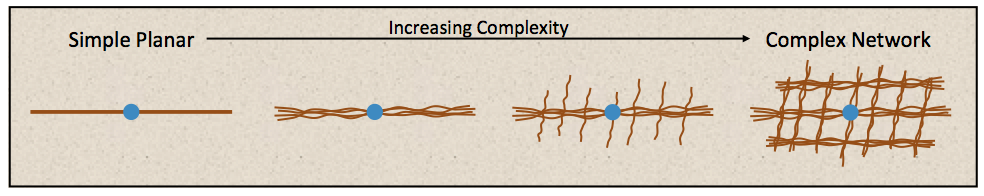
\includegraphics[width=\columnwidth]{figures/phys_prop_model/frac_complexity.png}
    \end{center}
\caption{
    Fracture complexity, from simple planar fractures on the left to complex fracture
    networks on the right. The blue doe is the injection point in a horizontal well. After \cite{Cipolla2008a}.
}
\label{fig:frac_complexity}
\end{figure}


To overcome these challenges, there are several approaches that may be taken; the appropriate choice will depend upon both the fracture complexity and the purpose of the simulation. If the fine-scale geometry of the fractures is defined, for example in a feasibility study built from a synthetic fracture model, then numerical upscaling \citep{Durlofsky2003, CaudilloMata2014, CaudilloMata2016} or multiscale techniques \citep{Haber2014} can be employed. In general, though, the fine-scale fracture geometry is not known; only a handful of studies have ``ground-truthed'' the geometry of an induced fracture by mining the fractured region \citep{Cipolla2008a}. Furthermore, in an inversion, we cannot expect to resolve individual fractures, rather, I aim to characterize the bulk impact due to electrically conductive fractures in a conductive medium. To estimate a bulk conductivity, effective medium theory is one approach that can be taken (c.f. \cite{Torquato2002, Milton2002, Berryman2013}). These methods assume that the composite material is composed of a collection of randomly distributed spheres or ellipsoids (which may be preferentially aligned). The estimated conductivity depends upon the conductivity of each of the materials, their shape, and volume in the composite material. Looking forward to the inverse problem, these methods have the added benefit that they provide a conduit for incorporating a-priori information such as expected primary-fracture orientation, and volumes of proppant and fluid.

In this work, I adopt an effective medium theory approach. I take into account the conductivity of the host rock, the fracturing fluid and the proppant. The main simplifying assumption I employ is on the geometry of the fractures: I assume that they are composed of a collection of ellipsoidal cracks which may be preferentially or randomly aligned. The derivation I present follows similar derivations presented in the literature (in particular, \cite{Torquato2002}), here I include details for preferentially aligned fractures resulting in a fully anisotropic conductivity.
\subsection{Chapter overview}
The purpose of this chapter is twofold: (1) I develop a workflow for estimating the physical properties of a fractured volume of rock containing proppant and fluid that have distinct electromagnetic properties from the host and (2) I assess if, using a commercially available electromagnetic survey, we can detect the anomaly introduced by the fracture in the data. All of the computations shown in this chapter are open-source and available as Jupyter notebooks (see Appendix \ref{app:code_list}).

\section{Homogenization workflow using effective medium theory}

In this approach, I treat the fractures as being composed of a collection of preferentially (or randomly) oriented ellipsoidal cracks and based on the density of cracks within a given volume of rock, construct an anisotropic description of the coarse-scale conductivity.

Effective medium approximations range from applying simple harmonic or arithmetic averaging of conductivity values, for example when constructing a representative voxel conductivity model from well-log measurements, to more involved analytic or empirical relationships such as Archie’s law \citep{Archie1942}, which is commonly applied for estimating the conductivity of a fluid-filled rock. Although discovered empirically, the simplest version of Archie’s law is one example of a differential effective medium approximation which can be derived analytically. It assumes a background matrix, and uses an incremental approach to constructing a homogenized conductivity (c.f. \cite{Torquato2002, Milton2002}). However, for describing a fractured volume of rock, differential effective medium approximations are not appropriate as they assume that the rock-matrix is always connected \citep{Torquato2002}; in the composite material we are considering, a single computational voxel may be intersected by a fracture, meaning the rock matrix is not connected. The Maxwell-approximation \citep{Maxwell1873} is yet another effective-medium approximation. It again makes a distinction between the background and the included phases, and assumes no interaction between inclusions.

I opt to consider self-consistent effective medium theory (SCEMT, also sometimes referred to as the Coherent Potential Approximation, CPS, or Bruggeman mixing). This is an effective medium approach which makes no distinction between background and included phases (e.g. see \cite{Torquato2002}). \cite{Berryman2013} similarly suggest using self-consistent effective medium theory for fractured rocks where the fractures are filled with fluid.

\cite{Milton1985} demonstrated the physical realizability of SCEMT; he showed that SCEMT is asymptotically the exact solution for the effective conductivity for fractal-like composites that are self-similar at many scales. Physical realizability means that the estimates given by SCEMT will always be within the Hashin-Shtrikman bounds; at a minimum, this provides confidence that the conductivity estimates it provides are physically within a reasonable relm.

I construct the physical property model for a fractured volume of rock in two steps, as shown in Figure \ref{fig:effective_medium_theory}. Given the conductivity of the fluid and proppant particles, I estimate the effective conductivity, $\sigma_2$, of a mixture of proppant and fluid. Next, I treat the fracture as consisting of a collection of ellipsoidal cracks filled with the proppant-fluid mixture. The ellipsoidal cracks may be preferentially aligned in a single or multiple directions or they may be randomly oriented. In both cases, I use the self-consistent effective medium theory, originally due to \cite{Bruggeman1935} and further developed by \cite{Landauer1952, Landauer1978}. In the following sections, I develop the theory and demonstrate its application for computing the effective conductivity of a proppant-fluid mixture as well as a fractured volume of rock.


\begin{equation}
        \sum_{j = 1}^N \phi_j \left(\boldsymbol{\Sigma^*} - \sigma_j \mathbf{I}\right)\mathbf{R}^{(j,*)} = 0
\label{eq:effective_medium_theory}
\end{equation}


\subsection{Summary of self-consistent effective medium theory}
\label{sect:emt_math}

Chapter 18 of \cite{Torquato2002} provides an overview of effective medium theory approaches. The discussion presented in this section follows their presentation, but additionally considers preferentially aligned cracks, resulting in an anisotropic effective conductivity. \cite{Berryman2013} present a similar overview but introduces several simplifying assumptions tailored for estimating the effective conductivity of a naturally fractured rock where the fractures are a relatively small concentration with respect to the host rock. Here, I avoid such assumptions and work with the general formulation with the aim of being suitable for calculating both the effective conductivity of a proppant-fluid mixture as well as arbitrarily oriented fractures, each at potentially high concentrations.

Each material, or phase, in the composite is assumed to be made up of spherical or ellipsoidal particles with a known aspect ratio. Starting from the solution for a sphere or an ellipsoid in a uniform electric field, the effective conductivity of a heterogeneous medium is chosen to be the conductivity for which the average perturbation to the electric field -- the difference between the electric field in the homogenized medium and the true conductivity model -- is zero. That is,
\begin{equation}
        \sum_{j = 1}^N \phi_j \left(\boldsymbol{\Sigma^*} - \sigma_j \mathbf{I}\right)\mathbf{R}^{(j,*)} = 0
\label{eq:effective_medium_theory}
\end{equation}

where $N$ is the number of different phases of materials, $\varphi_j$ is the volume fraction of the $j$-th phase, and $\sigma_j$ is the electrical conductivity of the $j$-th phase. $\boldsymbol{\Sigma^*}$ is the $3 \times 3$ effective conductivity tensor, and $\mathbf{I}$ is the $3 \times 3$ identity matrix. The matrix $\mathbf{R}^{(j,*)}$ is the electric field concentration tensor, and depends both on the shape of the inclusions (ie. proppant particles or cracks composing a fracture) and conductivity of the $j$-th phase, as well as the effective conductivity $\boldsymbol{\Sigma^*}$.

For spherical particles, the electric field concentration tensor $\mathbf{R}^{(j,*)}$ reduces to a scalar, namely,
\begin{equation}
    \mathbf{R}^{(j,*)} = \left[\mathbf{I}+\frac{1}{3}\boldsymbol{\Sigma^*}^{-1}(\sigma_j\mathbf{I}-\boldsymbol{\Sigma^*})\right]^{-1}
\label{eq:emt_r_spheres}
\end{equation}

The resultant effective conductivity expression in \ref{eq:effective_medium_theory} then reduces to a scalar equation.

If instead ellipsoidal inclusions are considered, the electric field concentration tensor is given by
\begin{equation}
    \mathbf{R}^{(j,*)} = \left[\mathbf{I}+\mathbf{A}\boldsymbol{\Sigma^*}^{-1}(\sigma_j\mathbf{I}-\boldsymbol{\Sigma^*})\right]^{-1}
\label{eq:emt_r_ellipsoids}
\end{equation}

Where $\mathbf{A}$ is the de-polarization tensor. For simplicity, I will assume that we are working with spheroids, either oblate (pancake-like) or prolate (needle-like) spheroids which have two semi-axes that are equal. The general solution for spheroids with three distinct semi-axes is presented in chapter 17 of \cite{Torquato2002} and additionally discussed in \cite{Berryman2013}. For a spheroid with semi-axes $a_1 = a_2 = a$ and $a_3 = b$ that is aligned so that $a_3$ lies along the z-axis, the depolarization tensor is given by
\begin{equation}
    \mathbf{A} = \left[
    \begin{array}{ccc}
    Q & & \\
    & Q & \\
    & & 1-2Q
    \end{array}
    \right]
\label{eq:emt_depolarization_tensor}
\end{equation}

For prolate spheroids, with aspect ratio $\alpha = b/a > 1$, $Q$ is given by
\begin{equation}
    Q = \frac{1}{2}\left(
        1 +  \frac{1}{\alpha^2 - 1}\left[1 - \frac{1}{2\chi_b} \ln\left(\frac{1 + \chi_b}{1 - \chi_b}\right)\right]
    \right)
    \label{eq:emt_q_prolate_spheroid}
\end{equation}

and for oblate spheroids ($\alpha = b/a < 1$),
\begin{equation}
    Q = \frac{1}{2}\left(
        1 +  \frac{1}{\alpha^2 - 1}\left[1 - \frac{1}{\chi_a} \tan^{-1}\left(\chi_a\right)\right]
    \right)
    \label{eq:emt_q_oblate_spheroid}
\end{equation}

with
\begin{equation}
    \chi_a^2 = - \chi_b^2 = \frac{1}{\alpha^2} - 1
    \label{eq:emt_chi}
\end{equation}

For preferentially aligned spheroids, the matrix $\mathbf{A}$ can be rotated as to align with the spheroidal axis using standard coordinate rotations. If the spheroids are randomly oriented, then we replace $\mathbf{R}^{(j,*)}$ with $1/3\text{trace}(\mathbf{R}^{(j,*)})$ in equation \ref{eq:effective_medium_theory}, and the effective conductivity expression reduces to a scalar equation. Note, that for spherical inclusions, $Q = 1/3$ and thus $\mathbf{A}$ reduces to a scalar equal to 1/3, showing that \ref{eq:emt_r_ellipsoids} is consistent with \ref{eq:emt_r_spheres}.

To solve for the effective conductivity, which is an implicit expression for $\Sigma^*$, we rearrange equation \ref{eq:effective_medium_theory} to
    \begin{equation}
        \Sigma^*\sum_{j=0}^N \varphi_j\mathbf{R}^{(j,\ast)} = \sum_{j=0}^N \varphi_j\sigma_j\mathbf{R}^{(j, \ast)}
    \label{eq:emt_solving_a}
    \end{equation}

and solve
    \begin{equation}
        \Sigma^* = \sum_{j=0}^N \varphi_j\sigma_j\mathbf{R}^{(j, \ast)} \left(\sum_{j=0}^N \varphi_j\mathbf{R}^{(j,\ast)}\right)^{-1}
    \label{eq:emt_solving_b}
    \end{equation}

using fixed-point iteration as $\mathbf{R}^{(j, *)}$ depends on $\Sigma^*$. Gradient-based optimization techniques could additionally be considered to speed-up convergence, but as this is a simple $3\times3$ matrix equation and the fixed-point iteration is sufficiently fast for the problems I consider. Note that the matrix inverse in \ref{eq:emt_solving_b} is a $3\times 3$ matrix inverse and thus is cheap to explicitly compute. The fixed-point iteration is performed until the recovered effective conductivity converges within a predefined tolerance. \cite{Berryman2013} similarly use a fixed-point iteration to solve for the effective conductivity, however in their formulation, they isolate $\Sigma^*$ by pulling out the first term in the summation in \ref{eq:effective_medium_theory}, leading to an update of the form
\begin{displaymath}
\Sigma^\ast = \sigma_0\mathbf{I} - \frac{1}{\phi_0}{\mathbf{R}^{(0,\ast)}}^{-1} \sum_{j=1}^N \phi_j(\Sigma^\ast-\sigma_j\mathbf{I})\mathbf{R}^{(j,*)}
\label{eq:emt_berryman_update}
\end{displaymath}



This is equivalent to equation 10 in \cite{Berryman2013} with the simplifications that $\mathbf{R}^{(j, *)}$ is replaced by $\mathbf{R}^{(j, 0)}$ under the assumption that the fractures compose a small volume fraction of the fractured rock. In practice, this approach is suitable for low concentrations of included phases, but can cause instability in the algorithm at higher concentrations (it is possible for updates to be negative, and therefore unphysical); the authors noted challenges with algorithm convergence when the concentration of inclusions exceeded 0.2.

In the following sections, I use this formulation to estimate the effective conductivity of a range of proppant-fluid mixtures as well as for a fractured volume of rock.

\subsection{Step 1: Effective conductivity of a proppant-fluid mixture}
In general, an induced fracture will be filled with two types or phases of material: proppant and fluid. Often this mixture is referred to as a slurry. There are two principal types of mixtures I will consider, one where all of the proppant is conductive, and the second when there is a conductive filler added to a conventional proppant.

I start by considering the case of a proppant with uniform conductivity, for instance if a conductive proppant, or coated proppant were used. I assume the conductivity of the proppant is known; Appendix \ref{app:concentric_spheres} includes a derivation for an effective conductivity of two concentric spheres for the scenario where the conductivity of a proppant particle and its coating are known independently.

For spherical proppant particles, the tensor-values in equation \ref{eq:effective_medium_theory} reduces to a scalar-valued equation, and the resulting effective conductivity is isotropic. In Figure \ref{fig:emt_spherical_particles}, I show the effective conductivity found using equations \ref{eq:effective_medium_theory} and \ref{eq:emt_r_spheres} for a proppant-fluid mixture as the concentration of proppant in the mixture ($\varphi$) is varied. The conductivity of the fluid is 3 S/m (similar to that of sea-water), and the proppant conductivity is varied logarithmically from 10 S/m to $10^5$ S/m. For example, coke-breeze, a graphite based material has conductivities $\sim 3000$ S/m, and other authors have considered the use of contrast agents that reach conductivities of $10^5$ S/m \cite{Weiss2015} and $10^6$ S/m \cite{Pardo2013}, which are similar to the conductivity of steel.


\begin{figure}
    \begin{center}
    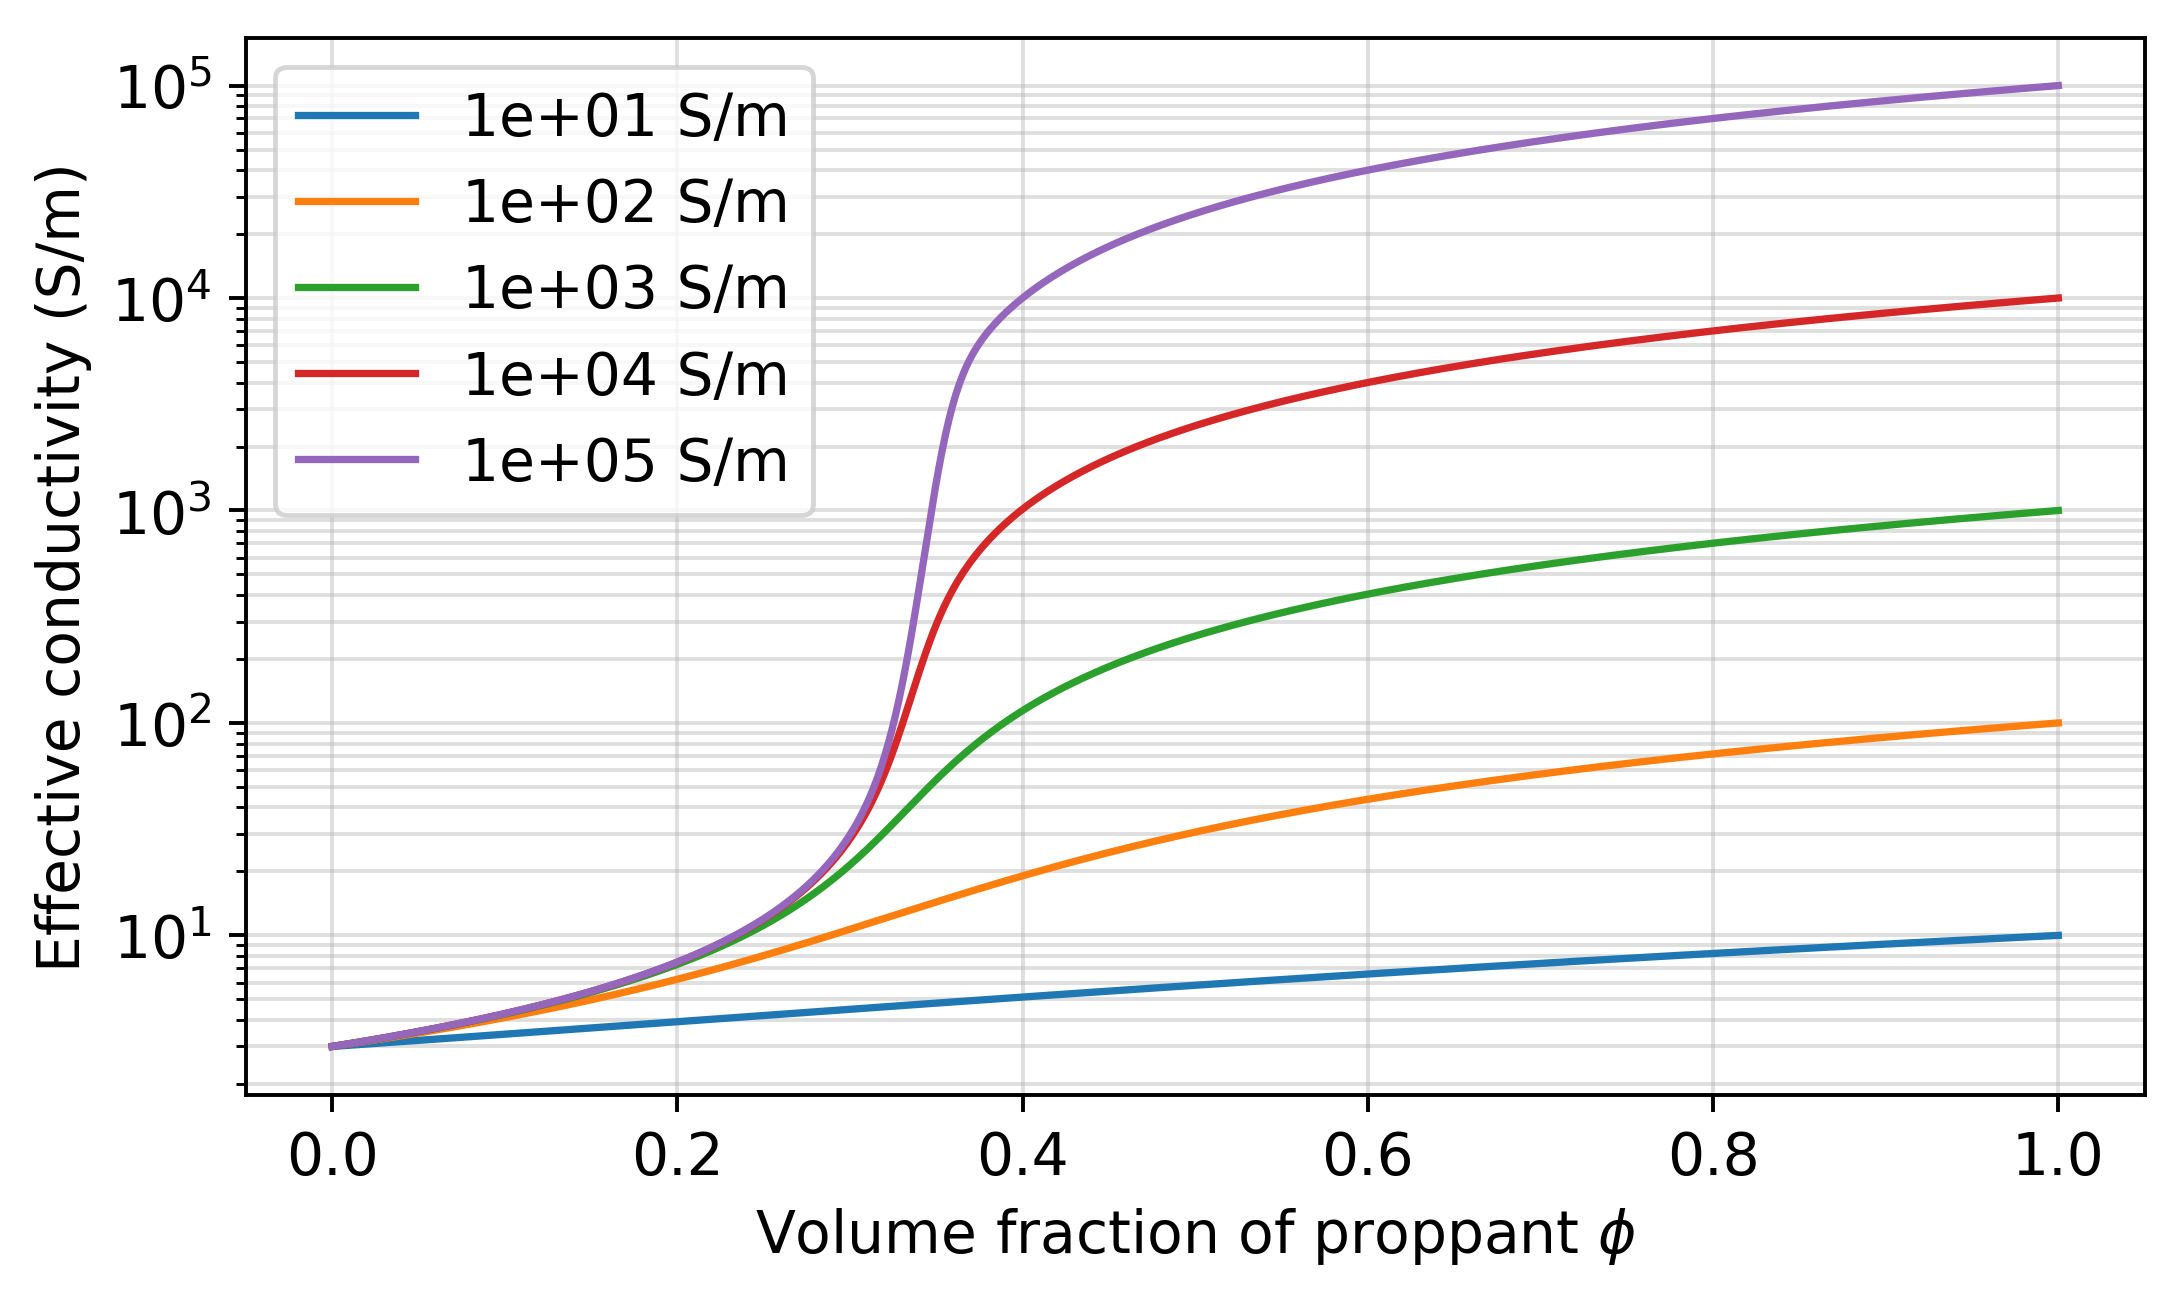
\includegraphics[width=0.6\textwidth]{figures/phys_prop_model/emt_spherical_particles.png}
    \end{center}
\caption{
    Effective conductivity of a proppant-fluid mixure for five different proppant
    conductivities, each indicated in the legend. Panel (a) shows the conductivity on a linear
    scale, and panel (b) uses a log-scale.
    The conductivity of the fluid is 3 S/m, similar to the conductivity of sea-water.
}
\label{fig:emt_spherical_particles}
\end{figure}


When the volume fraction of proppant is less than $1/3$, the conductivity of the fluid is the dominant control on the resulting effective conductivity. Above a volume  fraction of $1/3$, the conductivity of the proppant is the primary contributor to the effective conductivity. The threshold between these behaviors is the \emph{percolation threshold}. Below it, the concentration of conductive material is low enough that it is quite likely disconnected, above $1/3$, the concentration is high enough to start forming connected, electrically conductive pathways, causing a large jump in the effective conductivity of the system. Although proppant typically composes $10\%$ to $20\%$ of the injected slurry, some of the injected fluid leaks off into the surrounding geologic formation leaving proppant concentration that can be $50\%$ in the fractures \cite{Novotny1977, Hoversten2015}.

The conductivity of the fluid also changes the resultant effective conductivity of the mixture. In Figure \ref{fig:emt_fluid}, I compare the effective conductivity for a mixture of conductive proppant (panel (a): $10^3$ S/m, panel (b): $10^4$ S/m) and four different fluid conductivities, ranging from 0.3 S/m to 300 S/m, as indicated in the legend. Although the conductivity of the fluid makes a significant difference at low proppant concentrations, above the percolation threshold of 33\%, the curves start to converge, particularly when the contrast between the conductivity of the proppant and the fluid exceeds 3 orders of magnitude. Thus, if the proppant can be made sufficiently conductive, its conductivity will be the controlling factor on the effective conductivity of the slurry that remains in the fractures.


\begin{figure}
    \begin{center}
    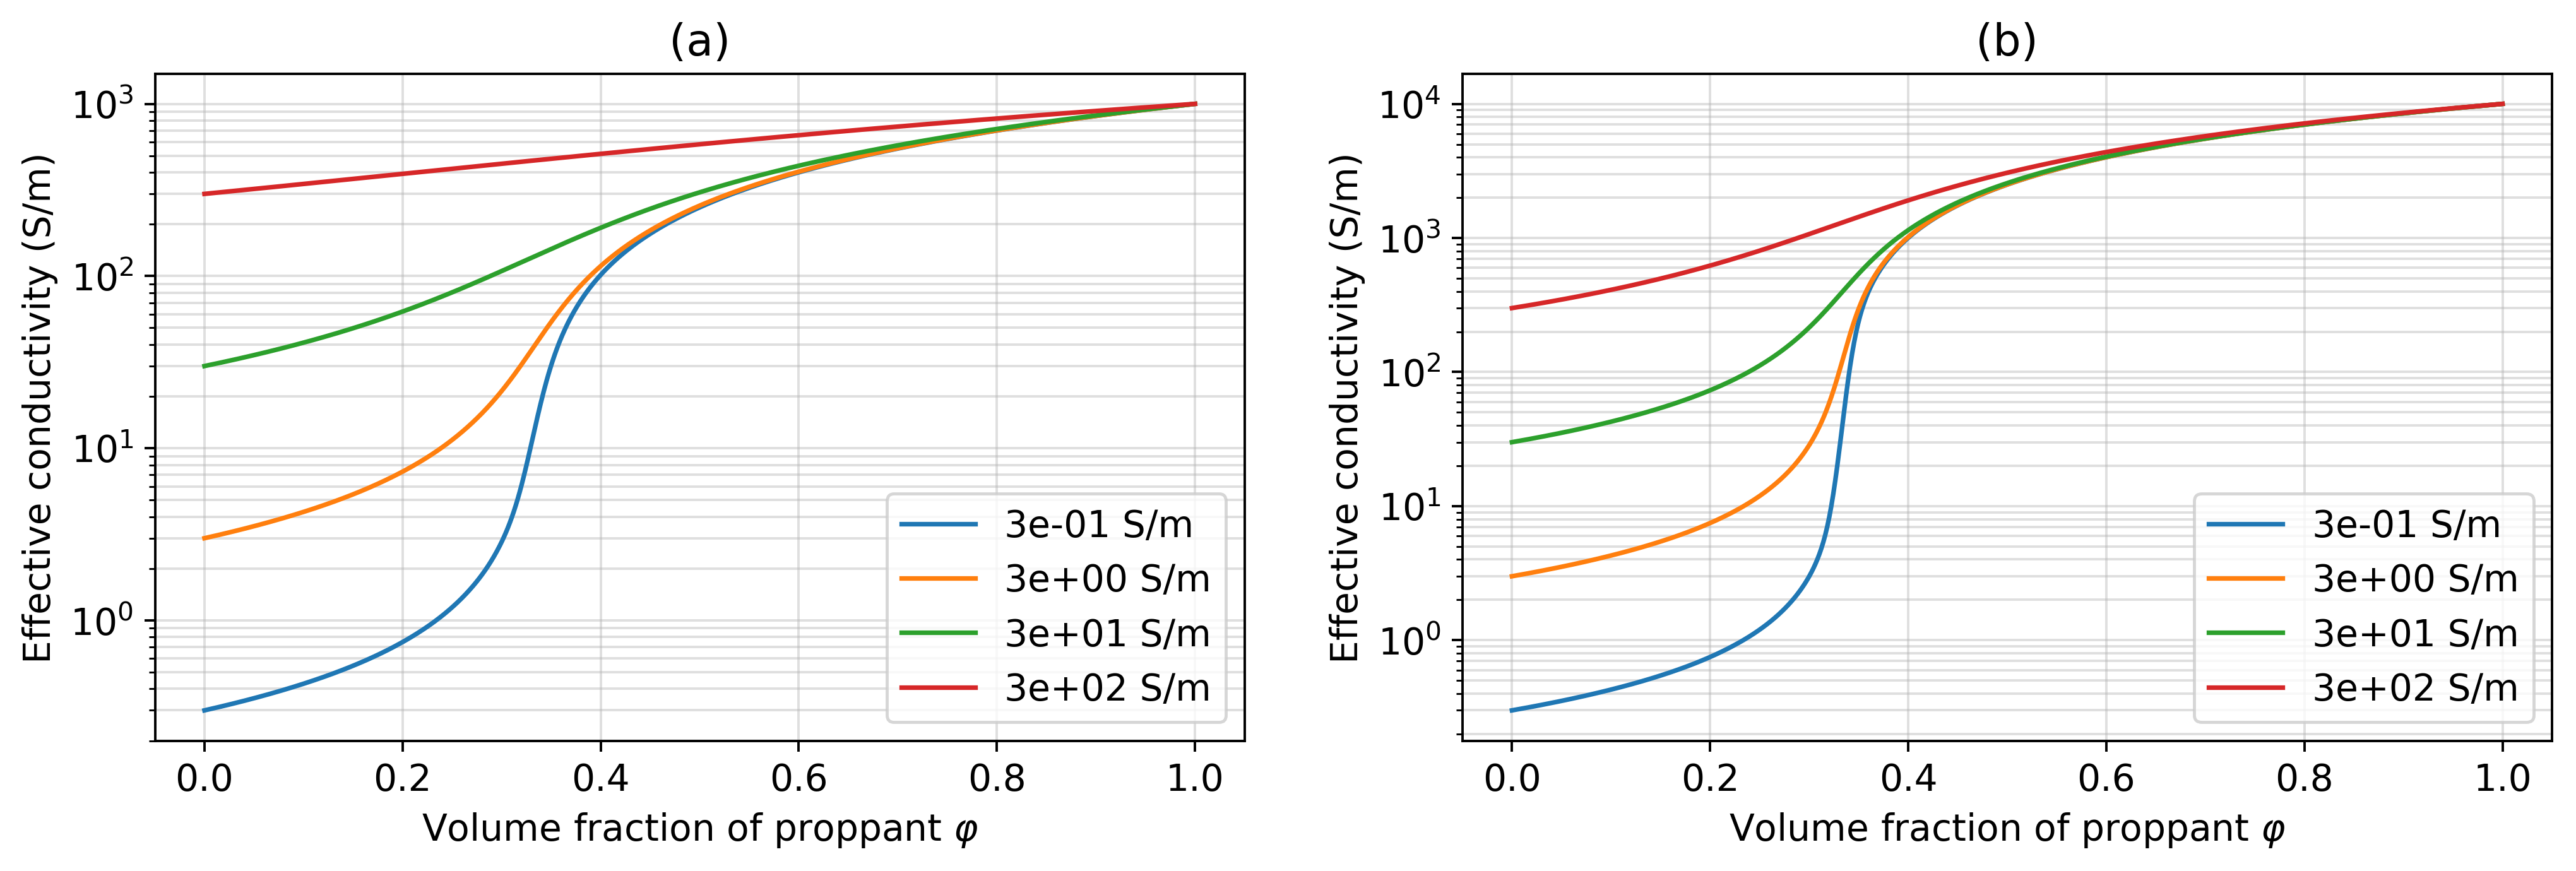
\includegraphics[width=\textwidth]{figures/phys_prop_model/emt_fluid.png}
    \end{center}
\caption{
    Impact of the conductivity of the fluid on the effective conductivity of a proppant-fluid mixture.
    Panels (a) and (c) show the effective conductivity for mixtures with a $10^3$ S/m proppant and panels
    (b) and (d) show the effective
    conductivity for mixtures with a $10^4$ S/m proppant. The conductivity of the fluid is indicated by the legend.
}
\label{fig:emt_fluid}
\end{figure}


The previous examples considered a 2-phase mixture in which all of the proppant was electrically conductive, however, depending on the setting and the cost to manufacture conductive proppant, it may be mixed in with conventional, resistive proppant. To examine this, I consider a proppant-fluid mixture composed of three materials, fluid ($3$ S/m), conventional, resistive proppant ($10^{-6}$ S/m) and conductive proppant ($10^5$ S/m). The effective conductivities of proppant-fluid mixtures for five different proppant blends, where the relative concentration of the conductive proppant is varied from 0\% to 100\% of the proppant phase, are shown in Figure \ref{fig:emt_3phase}. Again, we see the impacts of the percolation threshold; when the conductive proppant composes less than $1/3$ of the proppant pack, the effective conductivity is dominated by the resistive proppant. When the conductive proppant composes more than $1/3$ of the proppant pack, we see that with increasing proppant concentration, the effective conductivity of the mixture is dominated by the conductive proppant. However, the percolation threshold for each of these mixtures is different. This is because it is the volume-fraction of the conductive proppant in the three-phase mixture, not the ratio of proppant to fluid, that determines when connected, electrically conductive pathways may be formed.


\begin{figure}
    \begin{center}
    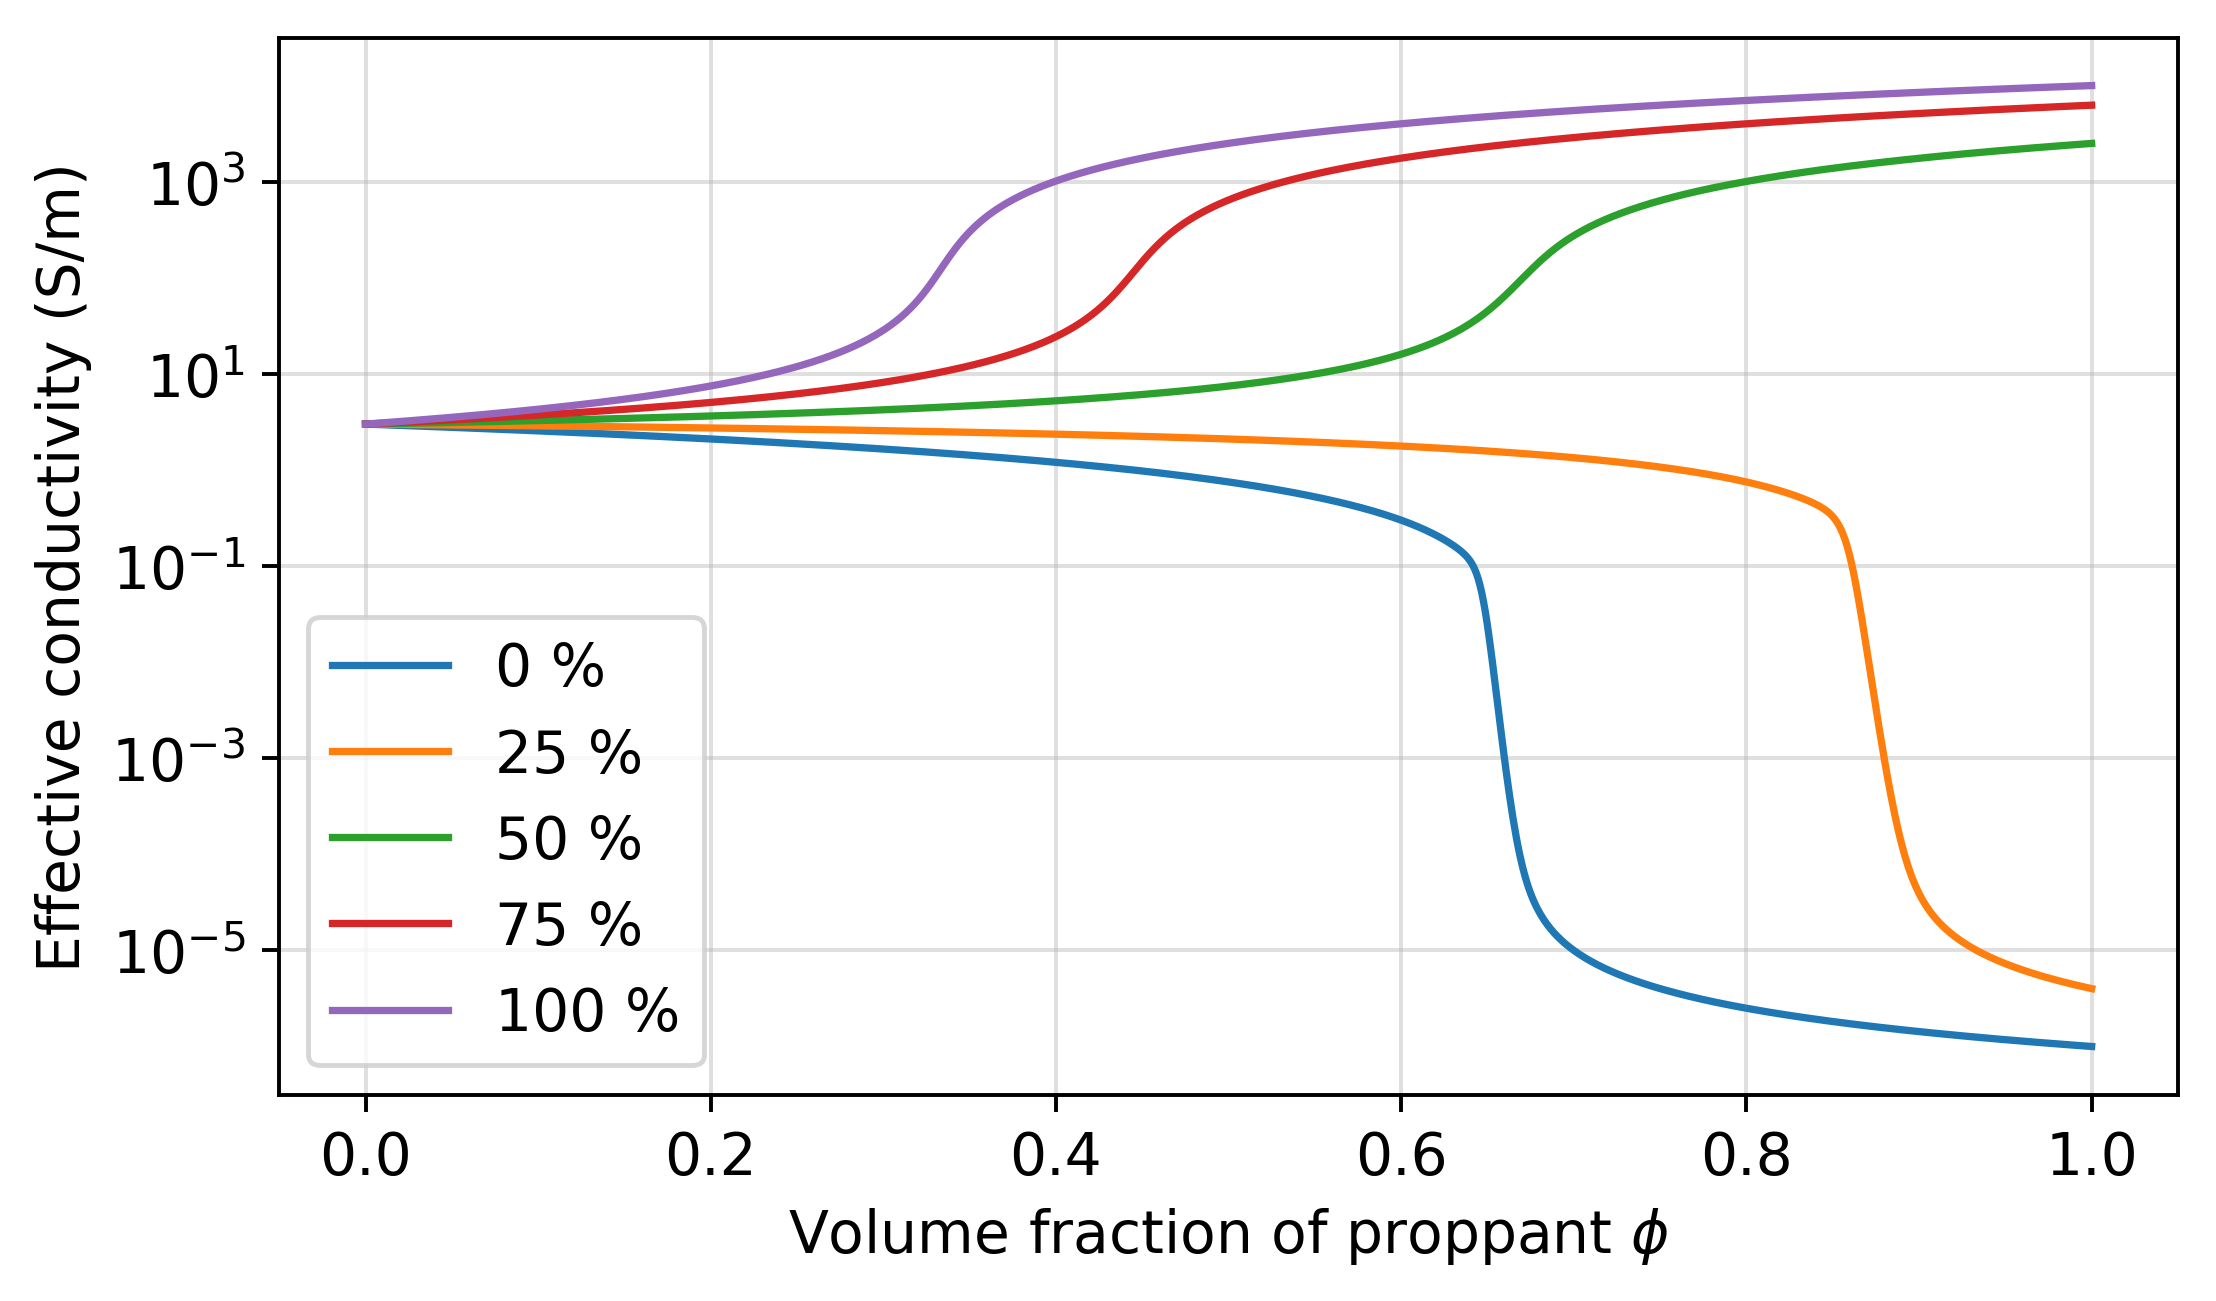
\includegraphics[width=0.6\textwidth]{figures/phys_prop_model/emt_3phase.png}
    \end{center}
\caption{
    Effective conductivity of a 3-phase proppant-fluid mixture consisting of
    resistive proppant ($10^{-6}$ S/m), conductive proppant ($10^5$ S/m) and saline
    fluid (3 S/m). The legend indicates the percentage of conductive proppant in the
    proppant mixture and the x-axis is the volume fraction of proppant in the
    proppant-fluid mixture.
}
\label{fig:emt_3phase}
\end{figure}


Another factor influencing the effective conductivity of a mixture is the shape of the materials. For the previous examples, the proppant was assumed to be composed of spherical particles. If elongated, conductive particles were included, we expect that connected, conductive pathways would form at lower concentrations. For instance, consider a 3 phase proppant mixture consisting of fluid (3 S/m), resistive, spherical proppant ($10^{-6}$ S/m), and elongated, electrically conductive proppant ($10^5$ S/m). Assume that the ratio of conductive to resistive proppant is 0.25 (below the percolation threshold for spherical particles). If the elongated particles (prolate spheroids) are randomly oriented, then the resulting effective conductivity is isotropic, meaning it is independent of the directions of the inducing field and resulting current. The conductivity predicted by effective medium theory for mixtures with five different aspect ratios is shown in figure \ref{fig:emt_3phase_aspect}. The aspect ratio of the conductive particles influences the concentration at which we observe percolation. The more elongated the particles, the lower the concentration at which percolation occurs.

\begin{figure}
    \begin{center}
    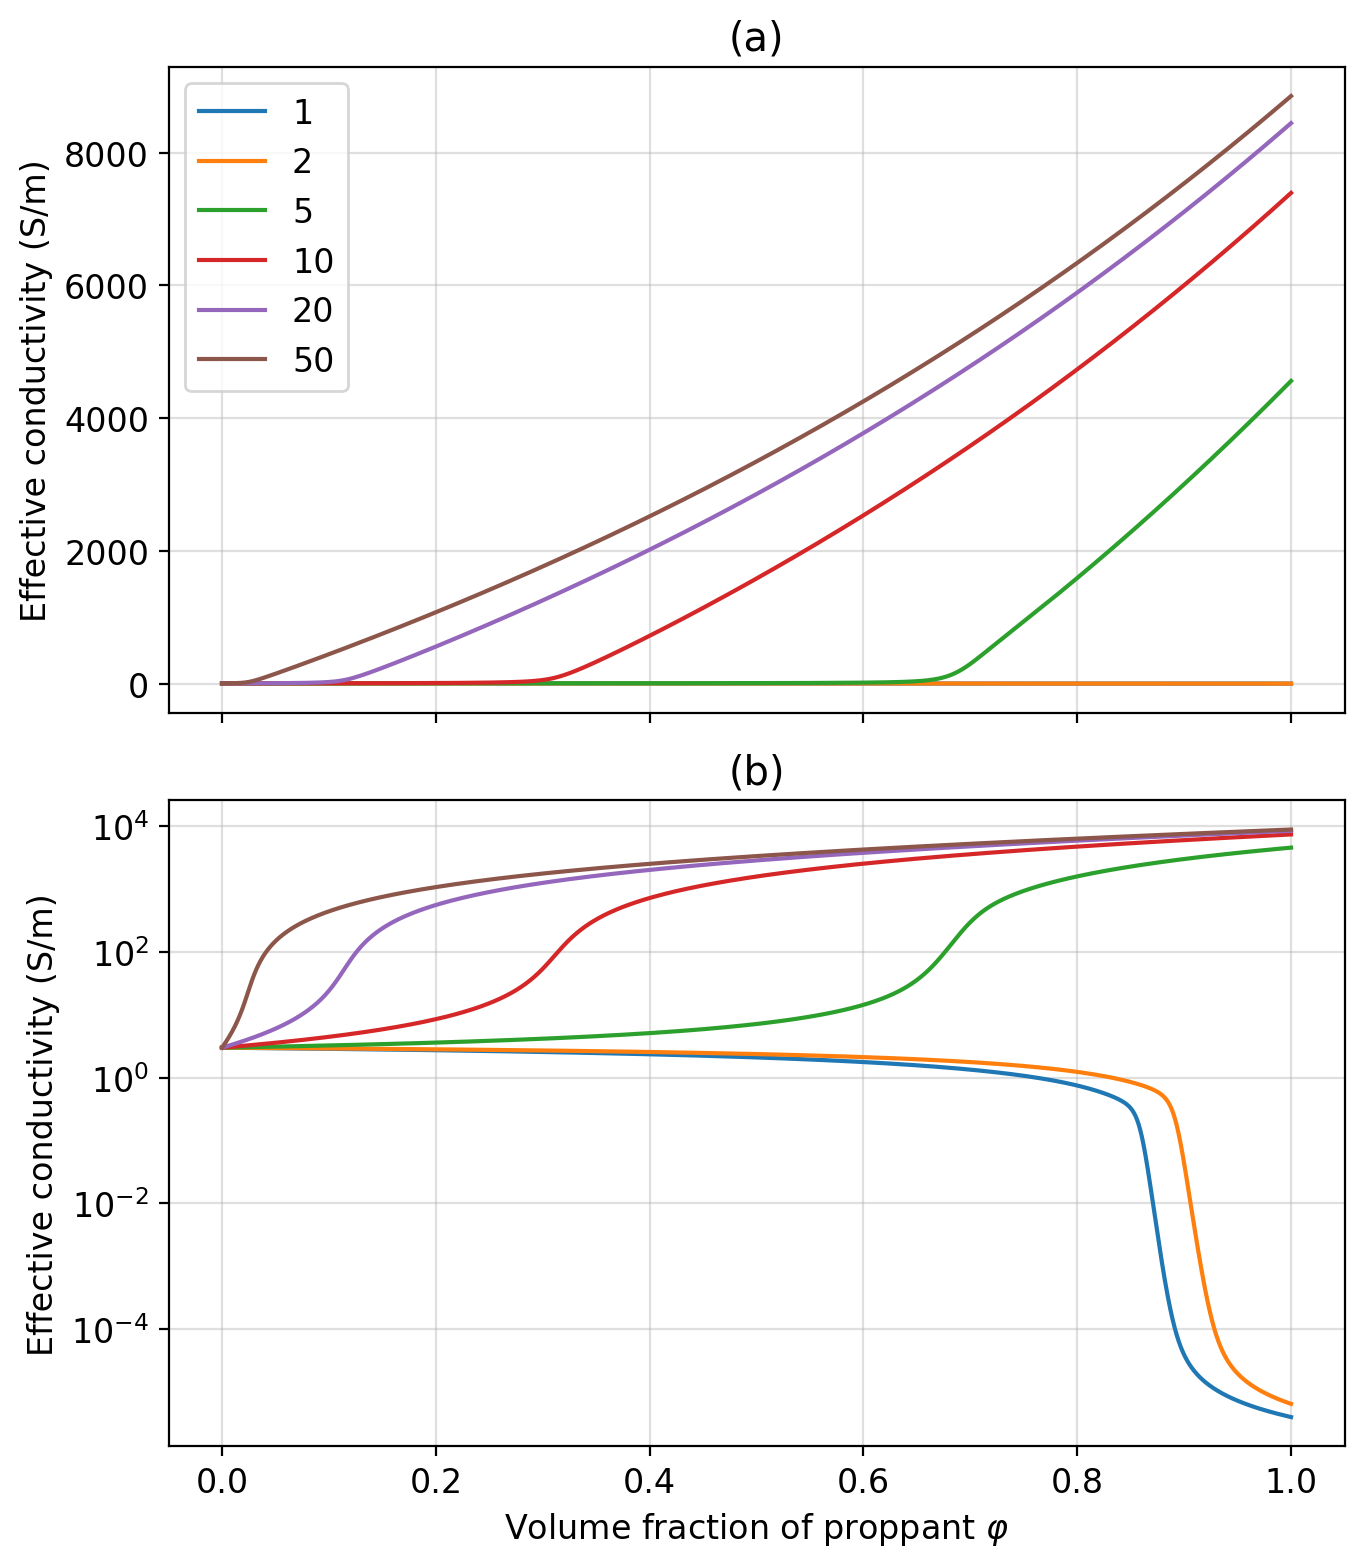
\includegraphics[width=0.6\textwidth]{figures/phys_prop_model/emt_3phase_aspect.png}
    \end{center}
\caption{
    Effective conductivity of a 3-phase proppant-fluid mixure consisting of
    resistive proppant ($10^{-6}$ S/m), conductive proppant ($10^5$ S/m) and saline
    fluid (3 S/m). The proppant mixture contains 25\% conductive proppant and
    75\% resistive proppant. The legend indicates the asppect ratio of the elongated
    conductive proppant filler (prolate spheroids).
}
\label{fig:emt_3phase_aspect}
\end{figure}


In summary, there are several approaches that can be taken to create an electrically conductive proppant-fluid mixture. Spherical proppant particles which are themselves electrically conductive or coated with a conductive material can comprise the entire proppant pack. If conductive proppant is mixed with a conventional, resistive sand or ceramic particles, then at least 1/3 of the proppant mixture needs to be comprised of electrically conductive particles to create a conductive mixture. This ratio can be reduced if elongated particles, such as metallic strips, are used in the proppant mixture.

\subsection{Step 2: Effective conductivity of fractured volume of rock}
\label{sec:emt-rock-volume}
The next step is to estimate the effective conductivity of a fractured volume of rock. I again employ self-consistent effective medium theory as described in section \ref{sect:emt_math} and consider the induced fractures to be composed of spheroidal cracks. Based on the analysis in the previous section, I consider a proppant-fluid mixture that has a conductivity of 2500 S/m. This could be achieved with spherical proppant particles having a conductivity of $10^4$ S/m in a 50/50 mixture with water of 3 S/m (see Figure \ref{fig:emt_spherical_particles}). Similar conductivities could be achieved with elongated particles mixed with conventional proppant as shown in Figure \ref{fig:emt_3phase_aspect}. Lab measurements conducted by \cite{Zhang2016} showed that a proppant-fluid mixture composed of petroleum coke particles and seawater which fills the pore-spaces reached a conductivity of $\sim 1000$ S/m at 37.6\% porosity. With further increase in confining pressure (thus reducing porosity and increasing the concentration of proppant), the observed conductivities range from  $3000 - 5000$ S/m. These results provide further confidence that conductivities $> 1000$ S/m for the mixture filling the hydraulic fractures are attainable.


For the following example, I will assume that the conductivity of the host-rock is 0.1 S/m. There are two scenarios I will consider, in the first, I assume the cracks are preferentially aligned, with the thin dimension of the oblate spheroid oriented along the x-axis, as shown in Figure \ref{fig:ellipsoid_geometry}. In this case, the recovered effective conductivity will be anisotropic, described by a diagonal matrix with entries $\sigma_y = \sigma_z \geq \sigma_x:$
\begin{equation}
    \Sigma^* = \left[
    \begin{array}{ccc}
    \sigma_x & & \\
    & \sigma_y & \\
    & & \sigma_z
    \end{array}
    \right]
    \label{eq:diagonal_sigma_e}
\end{equation}

Note that arbitrary, non-axes aligned, orientations can be considered; all that is required is that the depolarization tensor described in \ref{eq:emt_depolarization_tensor} is rotated to the desired orientation.


\begin{figure}
    \begin{center}
    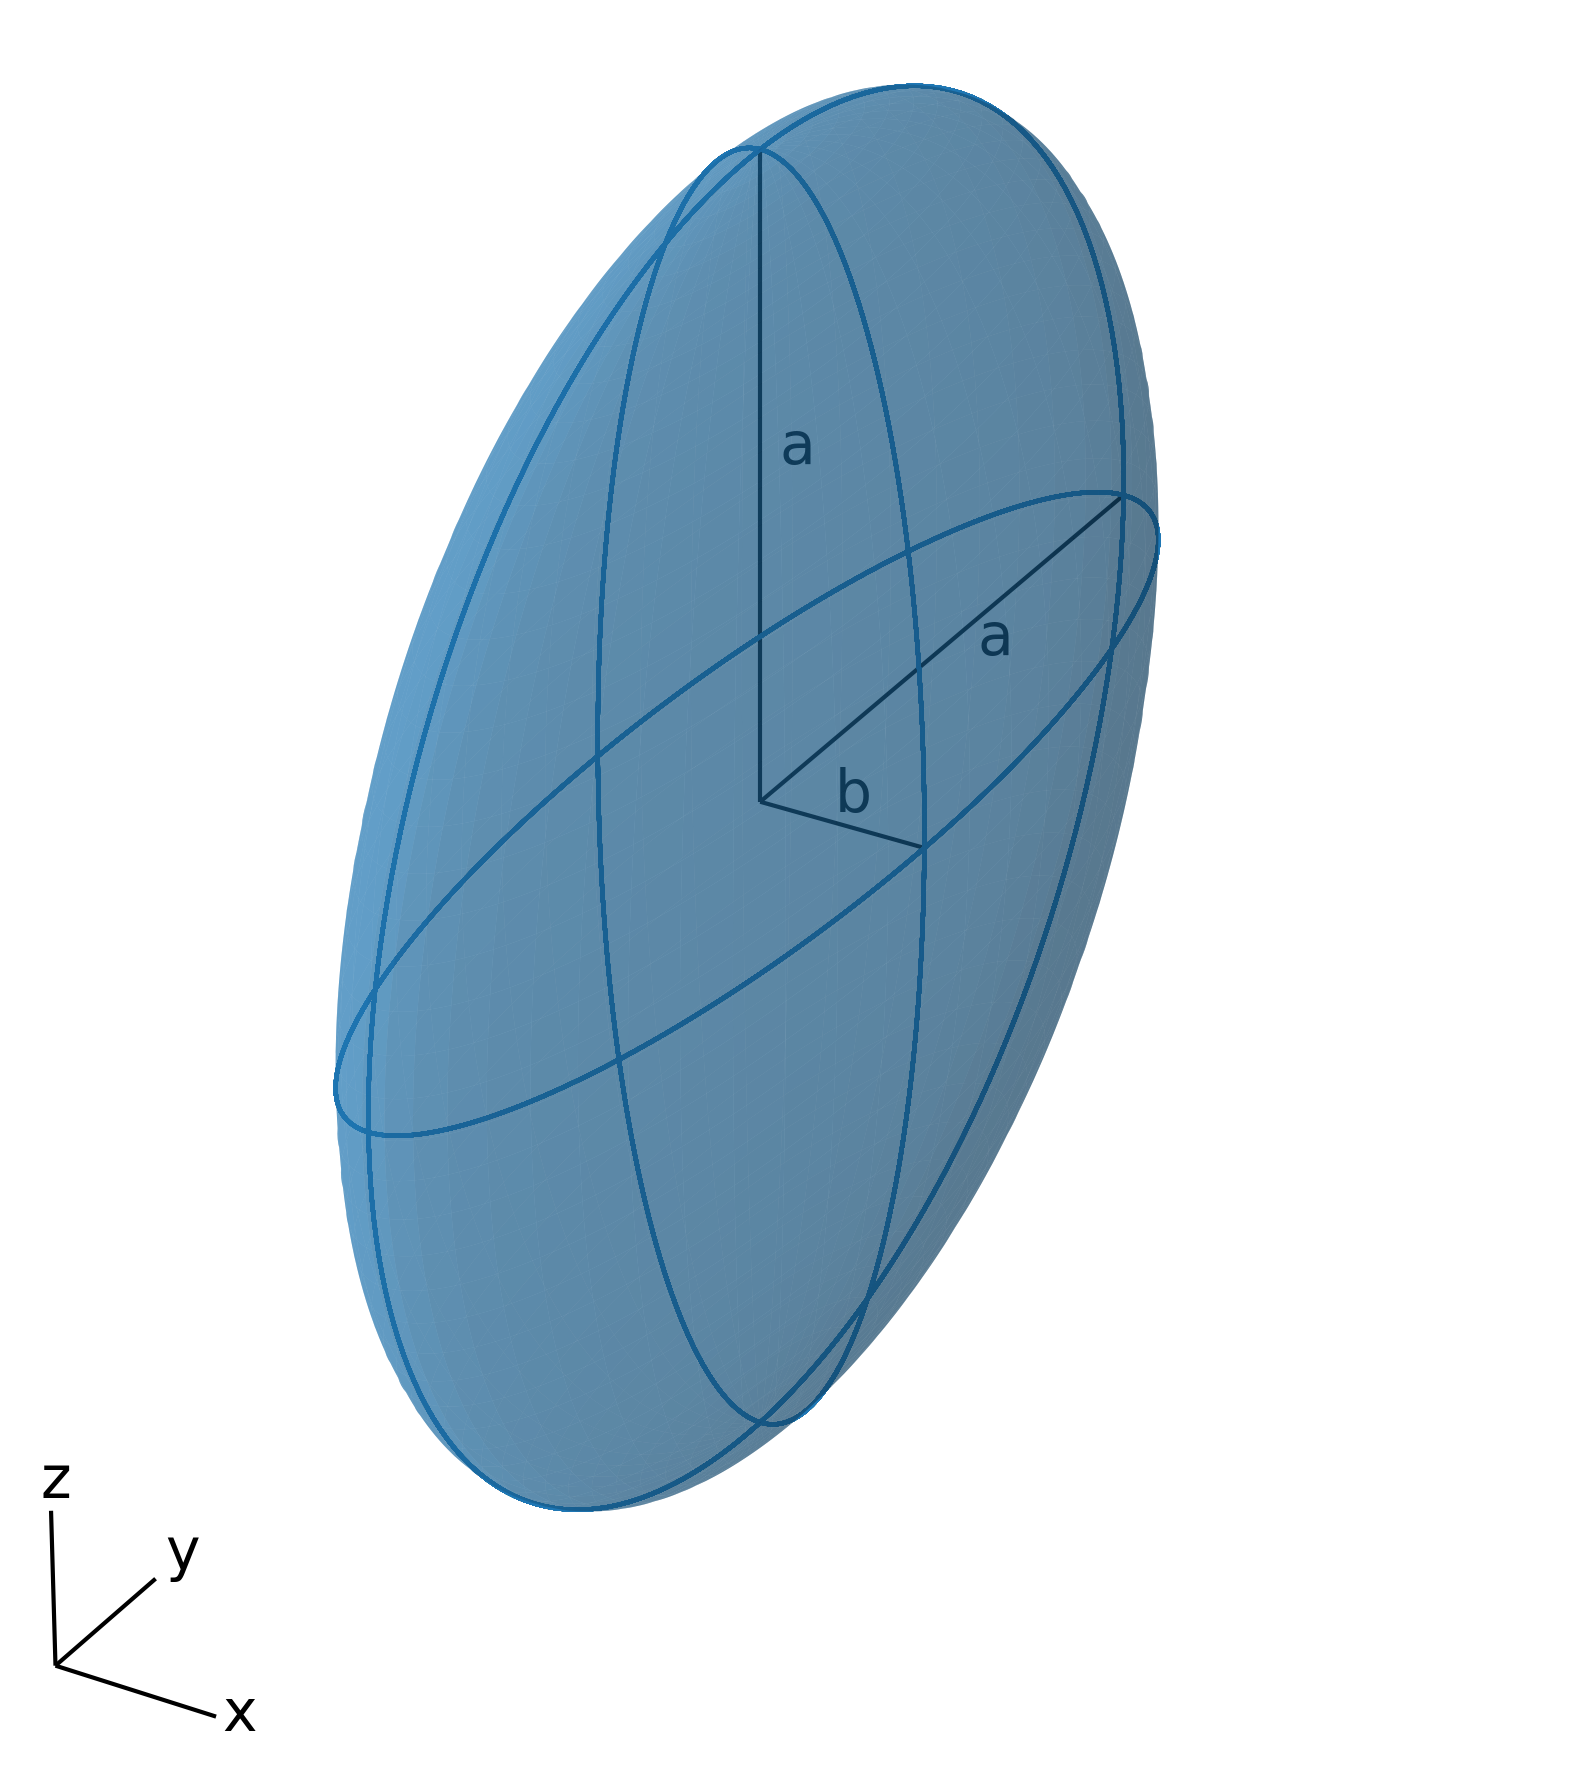
\includegraphics[width=0.5\columnwidth]{figures/phys_prop_model/ellipsoid_geometry.png}
    \end{center}
\caption{
    Oblate spheroid with normal along the $x$-axis. The $y$ and $z$ semi-axes are equal,
    and aspect ratio is $\alpha = b/a < 1$.
}
\label{fig:ellipsoid_geometry}
\end{figure}


To estimate the effective conductivity of a fractured volume of rock, we must also specify the aspect ratio of the cracks. In estimating this, assume a fractal-like approximation, where the aspect ratio of the fracture is representative of the aspect ratio of the cracks that compose it. For example, if the fracture extends 50m laterally and has a width on the order of millimeters, then the aspect ratio is on the order of $10^{-5}$. In Figure \ref{fig:aligned_fractures}, I have plotted the diagonal elements of the effective conductivity for five different aspect ratios, indicated in the legend, as a function of the volume fraction of conductive fractures in the rock volume sampled. Panel (a) shows the full range from $0 \leq \varphi \leq 1$ and panel (b) zooms in to lower concentrations ($0 \leq \varphi \leq 0.01$) which are more representative of a fractured rock volume, on the scale that we will consider for numerical modelling (e.g. if 10 fractures, each with 3mm width intersect a 10m $\times$ 10m $\times$ 10m cell, then $\varphi = 0.003$). In each of the plots, I have also included the upper and lower Wiener bounds (see equation 21.14 in \cite{Torquato2002}; originally attributed to \cite{Wiener1912}):
\begin{equation}
\begin{split}
\sigma_{\rm W}^{+} &= \sum_{j=0}^N \varphi_j \sigma_j \\
\sigma_{\rm W}^{-} &= \left(\sum_{j=0}^N \frac{\varphi_j}{\sigma_j}\right)^{-1}
\end{split}
\label{eq:wiener_bounds}
\end{equation}

in the black dashed lines; these can be understood as similar to parallel and series circuit approximations to the conductivity. In the black dash-dot lines are the upper and lower Hashin-Shtrikman bounds for 2-phase anisotropic media in the black dash-dot (see equations 21.25 and 21.26 in \cite{Torquato2002}, which is the anisotropic generalization of the isotropic bounds derived by \cite{Hashin1962}):
\begin{equation}
\begin{split}
\sigma_{\rm HS}^{+} &= \sigma_W^{+} \mathbf{I} + (\sigma_1 - \sigma_0)^2 \mathbf{\tilde{A}} \cdot
\left[\sigma_1\mathbf{I} + \frac{\sigma_1 - \sigma_0}{\varphi_0}\mathbf{\tilde{A}}\right]^{-1}\\
\sigma_{\rm HS}^{-} &= \sigma_W^{+} \mathbf{I} + (\sigma_1 - \sigma_0)^2 \mathbf{\tilde{A}} \cdot
\left[\sigma_0\mathbf{I} + \frac{\sigma_0 - \sigma_1}{\varphi_1}\mathbf{\tilde{A}}\right]^{-1}
\end{split}
\label{eq:hashin_shtrikman_bounds_anisotropic}
\end{equation}

For $\sigma_1 \geq \sigma_0$ and
\begin{equation}
\mathbf{\tilde{A}} = - \varphi_0\varphi_1\mathbf{A}_1
\label{eq:hashin_shtrikman_bounds_A}
\end{equation}

where $\mathbf{A}_1$ is the depolarization tensor for the ellipsoidal cracks given by equation \ref{eq:emt_depolarization_tensor}. For the bounds shown in the plot, the smallest aspect ratio, $10^{-5}$ was used to calculate the depolarization tensor. For the very significant aspect ratios used here, the Hashin-Shtrikman bounds are nearly identical to the Wiener bounds. Each component of the recovered effective conductivity should fall within these bounds.

\begin{figure}
    \begin{center}
    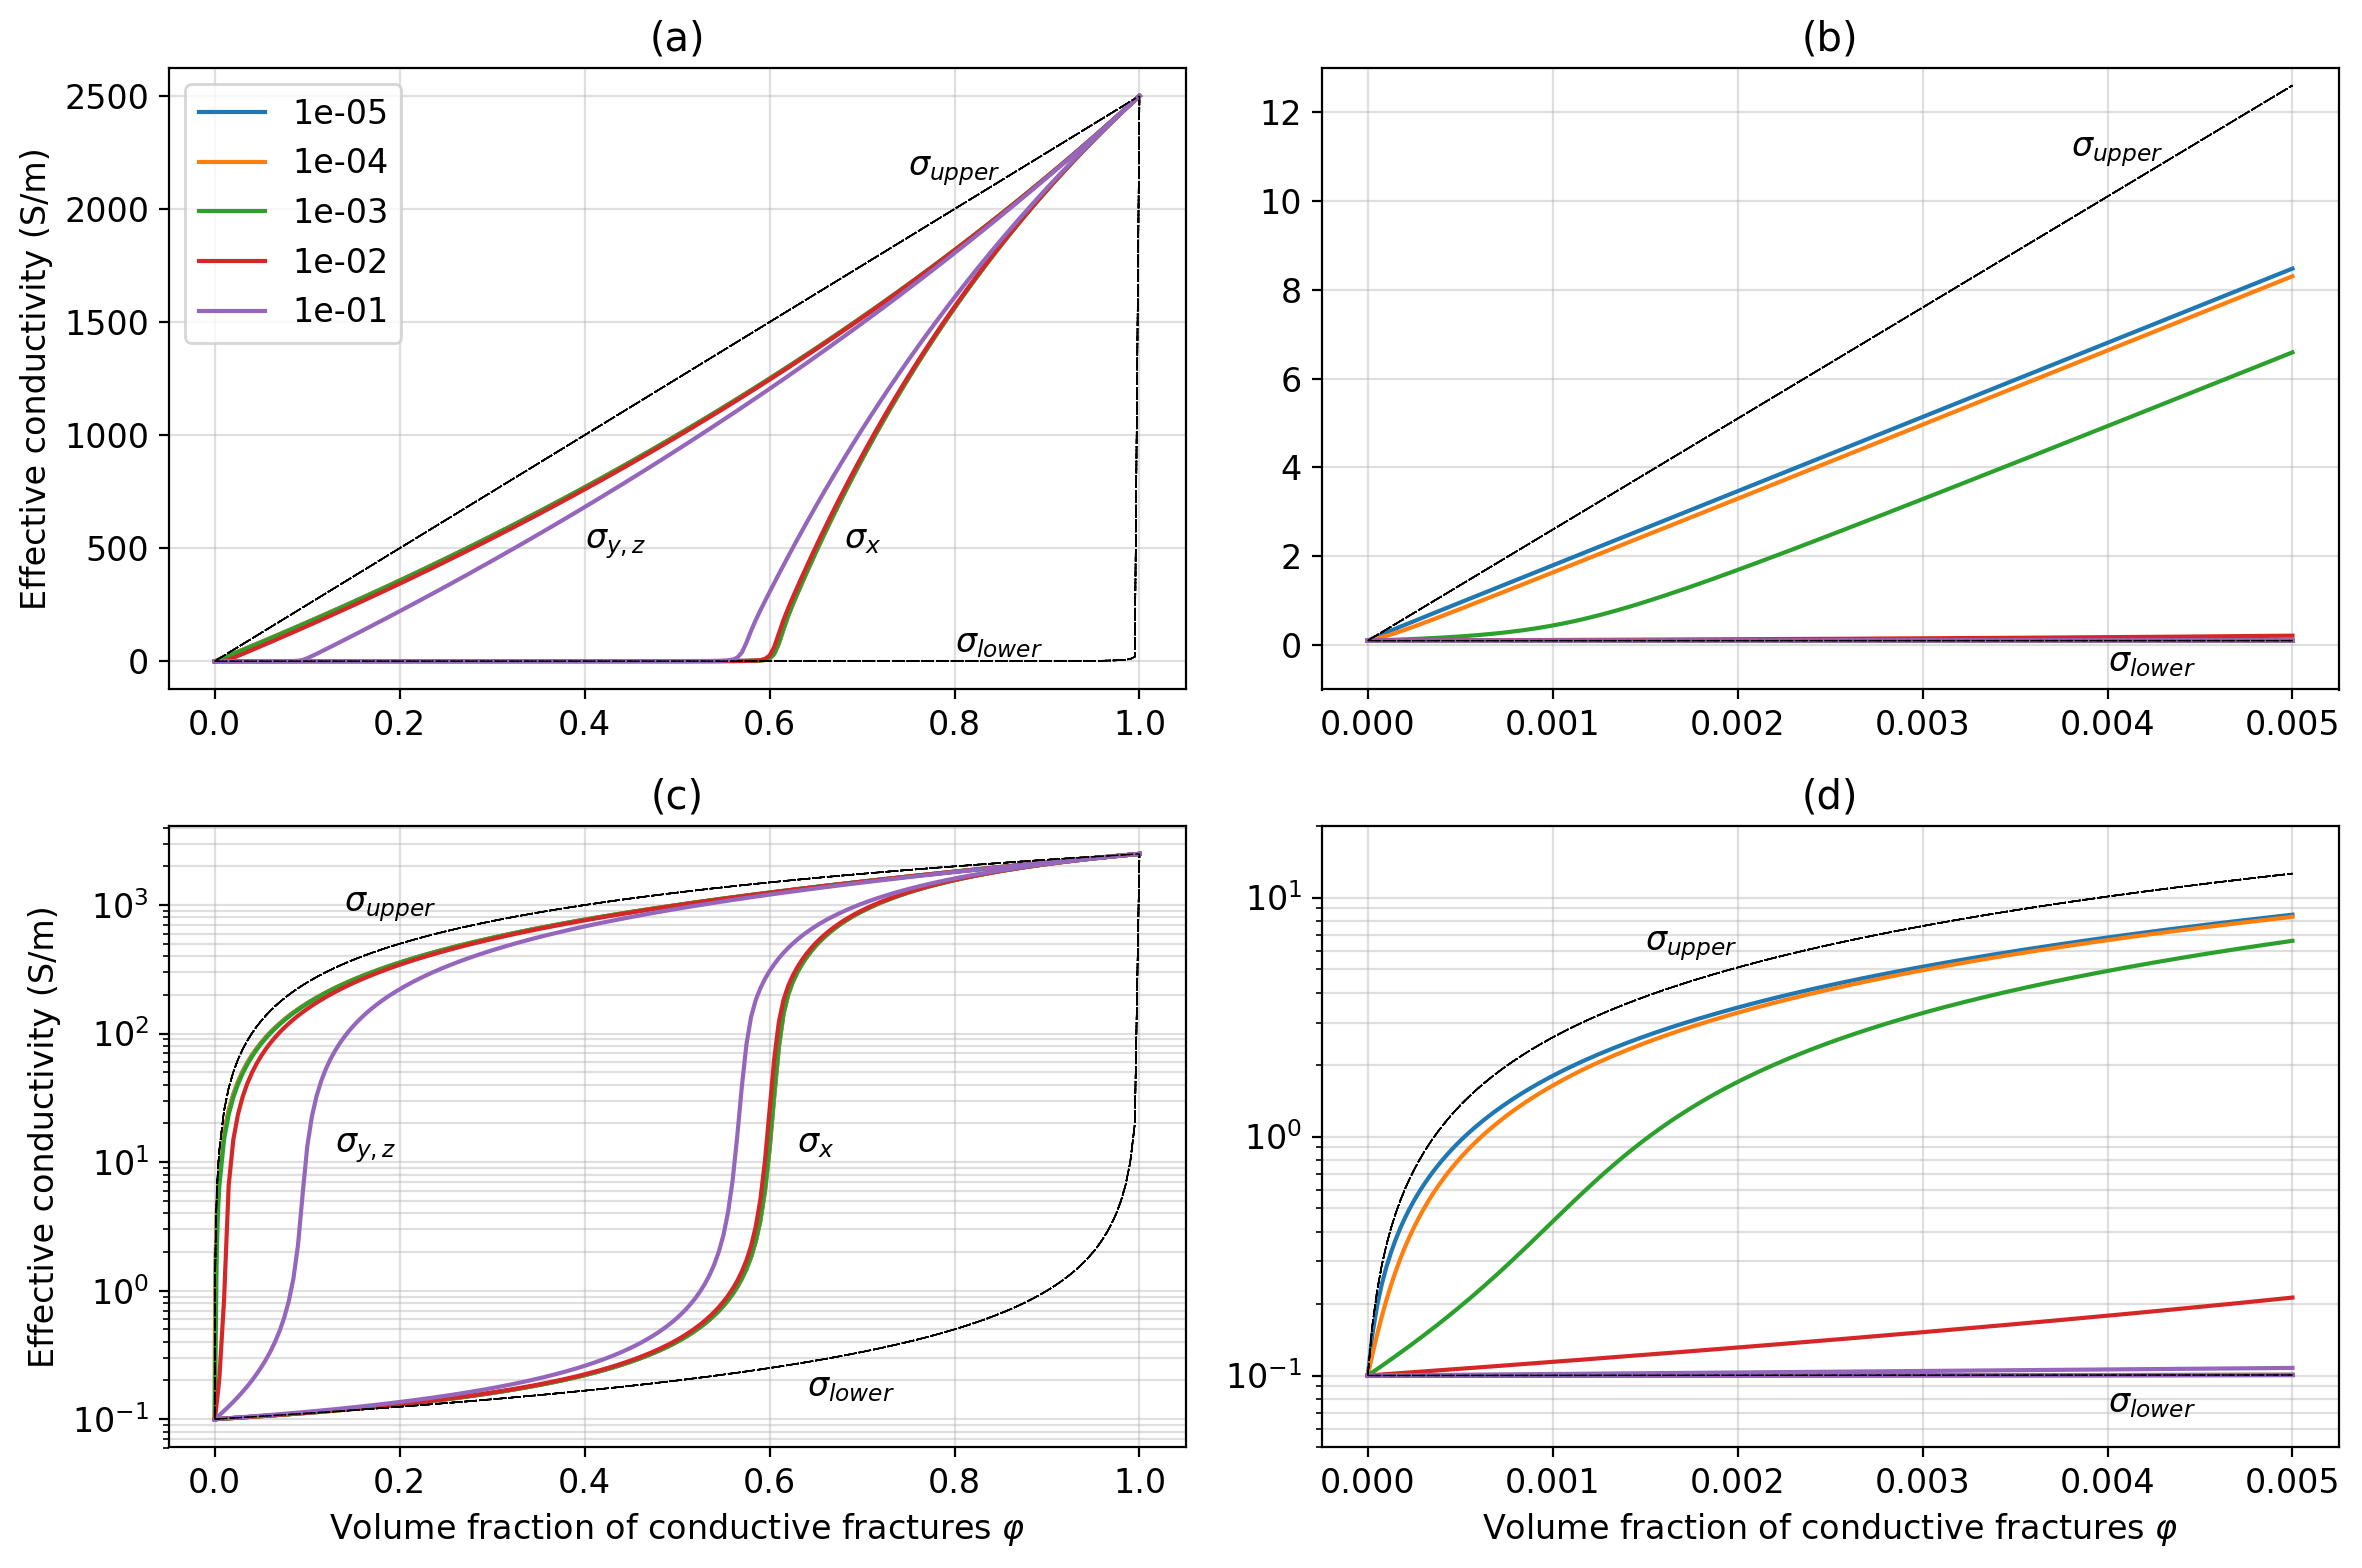
\includegraphics[width=\columnwidth]{figures/phys_prop_model/aligned_fractures.png}
    \end{center}
\caption{
    Effective, anisotropic conductivity for a fractured rock with spheroidal
    cracks whose normal is oriented along the x-axis for five different aspect ratios, indicated by the legend.
    The black dashed lines show the upper and lower
    Wiener Bounds, which are identical to the volume-weighted arithmetic and harmonic averages of the
    conductivity of the rock (0.1 S/m) and proppant-fluid mixture (2500 S/m). The black dash-dot lines
    are the anisotropic Hashin-Shtrikman upper and lower bounds computed using an aspect ratio of $10^{-5}$ in
    equation \ref{eq:hashin_shtrikman_bounds_anisotropic}. Note that the upper-bound coencides with $\sigma_{y, z}$ for small aspect ratios (e.g. the blue line).
    Panels (a) and (c) show the
    full range $0 \leq \varphi \leq 1$, and panels (b) and (d) zoom in to $0 \leq \varphi \leq 0.005$.
    Note that in (b), any curve that deviates from the lower bound is the $\sigma_{y, z}$ component;
    all $\sigma_x$ values lie on the lower bound for the concentration range shown.
}
\label{fig:aligned_fractures}
\end{figure}


For aspect ratios less than $10^{-3}$, we see very little distinction between the estimate of $\sigma_{y, z}$ and $\sigma_{x}$; the difference between the recovered effective conductivities for the aspect ratios of $10^{-4}$ and $10^{-5}$ is less than 1\% for all values of $\varphi$. This indicates that for sufficiently thin cracks, the exact aspect ratio is not critical for estimating a representative conductivity of the fractured rock.

At the concentrations we expect to be observing in a hydraulic fracturing scenario (Figure \ref{fig:aligned_fractures}b), we see that the effective conductivity along the normal of the fractures coincides with the lower bounds and remains nearly identical to the conductivity of the host rock for all aspect ratios shown, as may be expected. For the components of the conductivity along the cracks ($\sigma_{y, z}$), the effective conductivity mimics the behavior of the upper bounds. These components of the conductivity are similar to the behavior expected from a parallel-circuit approximation.

For settings where planar fractures are expected, a single orientation of the inclusions produces similar behavior to what would be expected if we performed simple series-and-parallel circuit approximations to the components perpendicular to and along the fracture. However, if more complex fracture networks are expected, it may be more appropriate to assume the cracks are randomly oriented. In this case, an isotropic conductivity describes the fractured volume of rock. Using the same aspect ratios shown in Figure \ref{fig:aligned_fractures} above, I compute the isotropic effective conductivity as a function volume fraction of fractures in Figure \ref{fig:random_fractures}. For reference, the conductivity along the fractures, $\sigma_{y, z}$ from Figure \ref{fig:aligned_fractures}, is plotted in semi-transparent lines. As in the previous Figure, panel (a) shows the full range from $0 \leq \varphi \leq 1$ and panel (b) zooms in to lower concentrations: $0 \leq \varphi \leq 0.01$.

\begin{figure}
    \begin{center}
    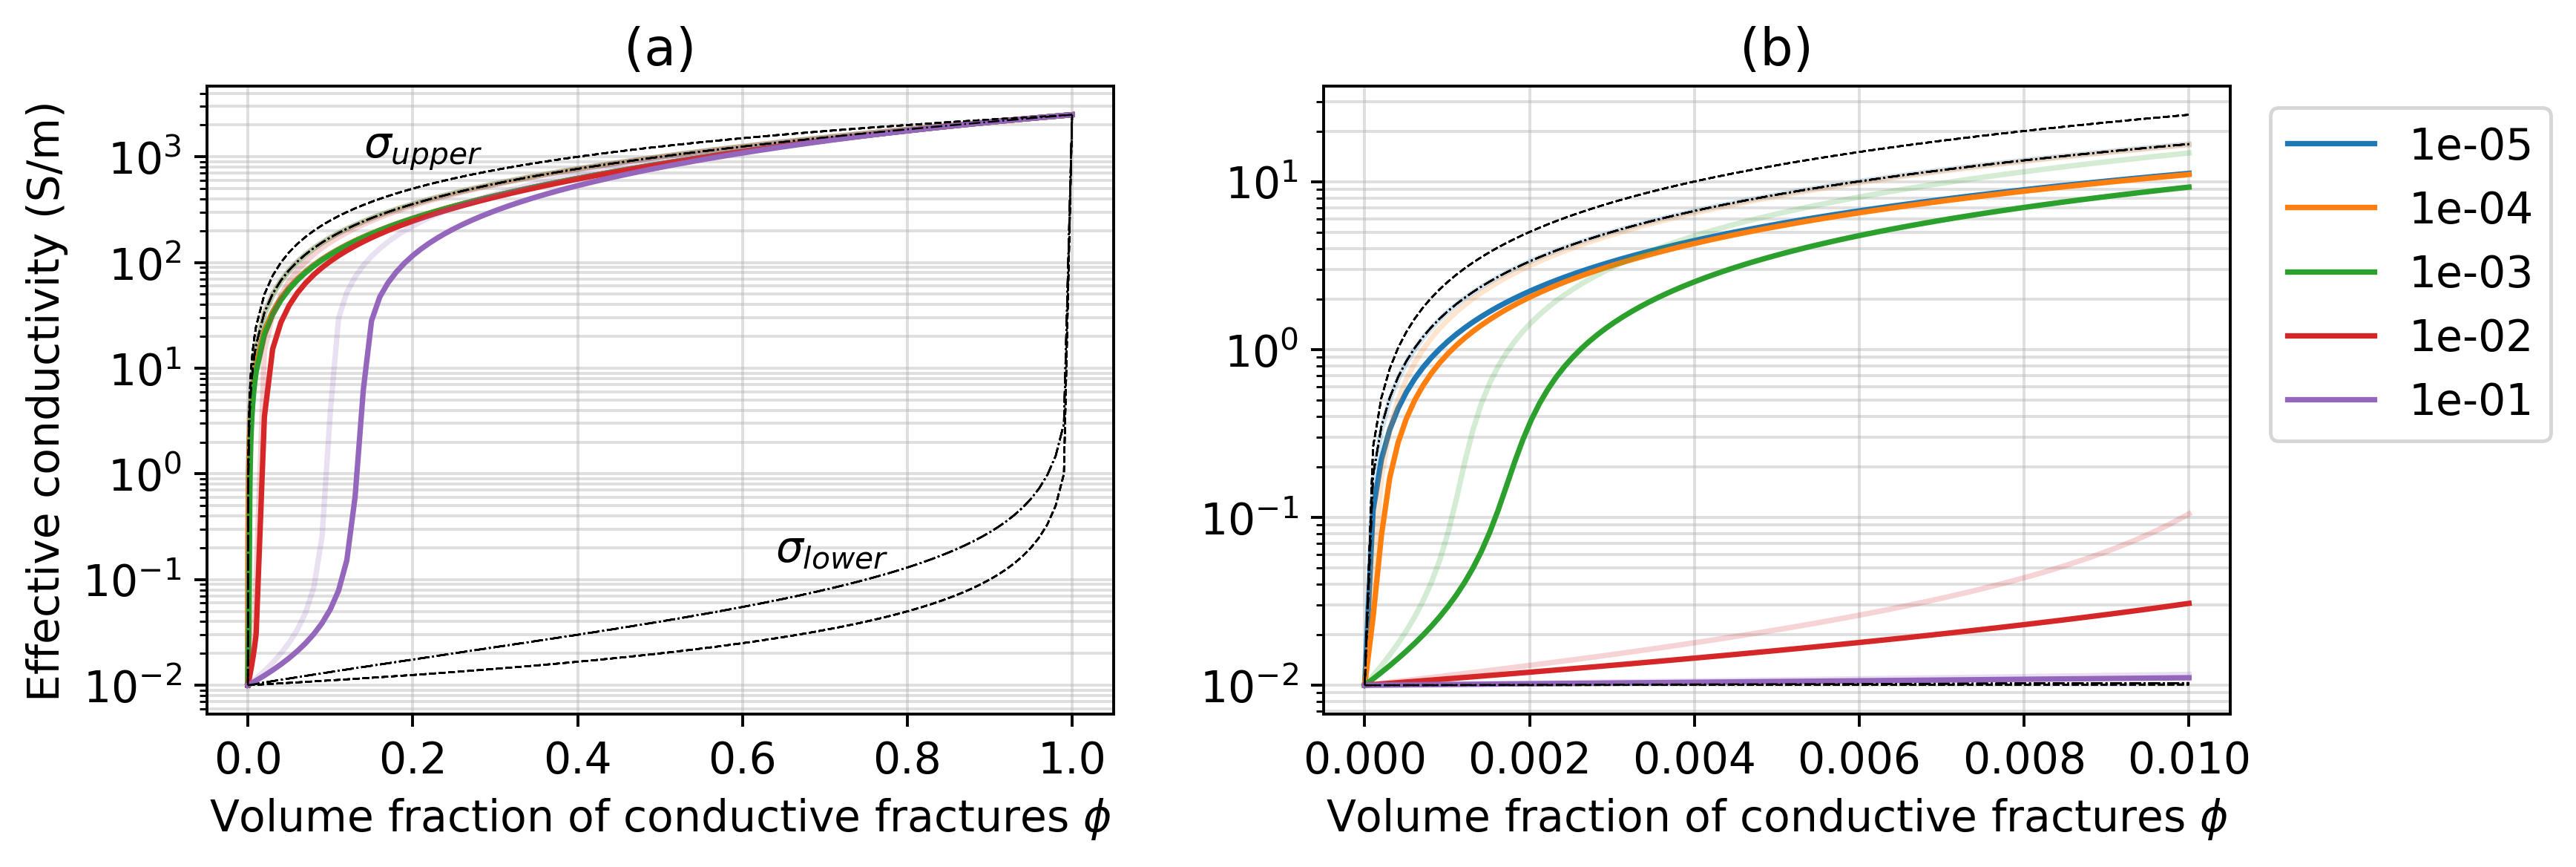
\includegraphics[width=\columnwidth]{figures/phys_prop_model/random_fractures.png}
    \end{center}
\caption{
    Effective, isotropic conductivity for a fractured rock with randomly oriented spheroidal
    cracks for five different aspect ratios, indicated by the legend. The black dashed lines show the upper and lower
    Wiener Bounds, which are identical the volume-weighted arithmetic and harmonic averages of the
    conductivity of the rock (0.1 S/m) and proppant-fluid mixture (2500 S/m).The black dash-dot lines
    are the isotropic Hashin-Shtrikman upper and lower bounds.
    The semi-transparent dotted lines show $\sigma_{y, z}$ from Figure \ref{fig:aligned_fractures}
    Panels (a) and (c) shows the
    full range $0 \leq \varphi \leq 1$, and panels (b) and (d) zooms in to $0 \leq \varphi \leq 0.01$.
}
\label{fig:random_fractures}
\end{figure}


Again, we see that for aspect ratios smaller than $10^{-3}$ there is little difference between the estimated effective conductivity of the fractured rock volume. The estimate of the effective conductivity largely follows the behavior of the upper bounds, while the magnitude of the effective conductivity is slightly reduced as compared to the component of the conductivity along the fractures in the anisotropic case. If we consider a $10m \times 10m \times 10m$ computational cell with fractures having an aspect ratio of $10^{-5}$ and composing 0.3\% of the total volume (e.g. 10 fractures, each with 3mm width), we obtain $\sigma_x = \sigma_z = 5.2$ S/m, $\sigma_y = 0.1$ S/m for the case where the cracks are preferentially aligned while for the case where the cracks are randomly oriented, we obtain $\sigma^* = 3.5$ S/m.

Due to the large contrast between the conductive fractures and the host rock, the conductivity of the background has marginal effect on $\sigma_{x, z}$ in the anisotropic example or on $\sigma^*$. If we consider the example with $\varphi = 0.003$, as before, and instead use a background conductivity of 0.01 S/m, the effective anisotropic conductivity is $\sigma_x = \sigma_z = 5.1$ S/m, $\sigma_y = 0.01$ S/m and for the isotropic case $\sigma^* = 3.4$ S/m. However, if the background is made more conductive and the contrast between the conductive fractures and the host reduced, we do see some impact. Setting the background to 1 S/m for this same example, we obtain $\sigma_x = \sigma_z = 6.4$ S/m, $\sigma_y = 1$ S/m for the anisotropic case and $\sigma^* = 4.7$ S/m for the isotropic case.


\subsection{Summary}
To construct an approximate conductivity model of a fractured volume of rock, I use a two step process: first, I estimate the effective conductivity of a mixture of proppant and fluid that fills the fractures and second, I estimate the effective conductivity of a fractured volume of rock.

In the section that follows, I will compare numerical simulations of a crosswell electromagnetic survey for both anisotropic and isotropic conductivity models of a fractured volume of rock, representing planar and complex fracture networks, respectively.

\section{Feasibility of EM for detecting fractures}
I now examine the feasibility of detecting a conductive, fractured region of a reservoir with an electromagnetic survey. The purpose of this section is to demonstrate detectability for a simple model of a fracture with existing electromagnetic imaging techniques. The survey I consider is a frequency-domain crosswell electromagnetic survey. In a crosswell EM survey a transmitter coil, which produces a time-varying magnetic field at a single frequency is positioned inside of one well. Time-varying magnetic fields induce time-varying currents in the earth whose distribution and magnitude depends upon the conductivity of the earth. These currents in turn generate secondary magnetic fields. In a second well, an array of receiver induction coils, which measure the time rate-of-change of the magnetic field (db/dt, in units of volts), are positioned. The measured voltages can be converted to magnetic field values. To conduct a survey, the position of the receivers is fixed and the transmitter is moved at a fixed rate along the borehole (typically 3-5 meters per minute). The receivers are repositioned, and the process repeated \citep{Wilt1995}. Both the transmitter and receivers are oriented along the axis of the borehole; for vertical wells, this means the transmitter is a vertical magnetic dipole, and the receivers measure the z-component of the magnetic field. Since its development, crosswell surveys have been used for a range of reservoir imaging problems for enhanced oil recovery including monitoring steam injections \citep{Wilt1997} and water floods \citep{Wilt2012}, including a survey conducted in a pair of horizontal wells \citep{Marsala2015, Marsala2015a}. In this section, I consider a crosswell survey and examine the feasibility of detecting signal due to a fractured volume of rock.

The setup I use is shown in Figure \ref{fig:crosswell_fractures}; a crosswell EM survey conducted in a pair of horizontal wells that are spaced 500m apart, as shown in Figure \ref{fig:crosswell_fractures}. The transmitter is oriented along the x-axis and positioned in the same well as where the fracture stimulation was performed; the receivers are in the offset well and measure the real and imaginary parts of the x-component of the magnetic field. In the numerical modelling, I assume that the wells are sufficiently deep so that the background can be treated as a whole-space. I do not consider steel-cased boreholes in this example and instead assume that the boreholes are open-holes or cased with fibreglass casing as in \cite{Wilt2012}. The additional complications due to steel cased wells will be discussed in the following three chapters.

Most hydraulic fracture operations involve injecting $\sim$800m$^3$ to 4000 m$^3$ (5000 to 25000 bbls) of proppant-fluid slurry into the reservoir rock, with the proppant comprising 10\% to 20\% of this mixture \citep{Hoversten2015}. In this example, I consider a fracture that is on the lower-end, with an 800m$^3$ slurry comprised of $15\%$ proppant by volume. A significant portion of the fluid typically leaks off into the surrounding formation \citep{Novotny1977}, so I will assume that the final mixture filling the cracks contains 50\% fluid and 50\% proppant. This gives a total fracture volume of 240 m$^3$. To distribute this volume, I assume that 10 fractures, each with 3mm width are positioned within a 10m interval along the well. Conserving volume and assuming circular fractures gives us a 50 m radius for each of the 10 fractures; I work with circular fractures as the resultant model is cylindrically symmetric, which significantly reduces the computational cost of the simulation.

\begin{figure}
    \begin{center}
    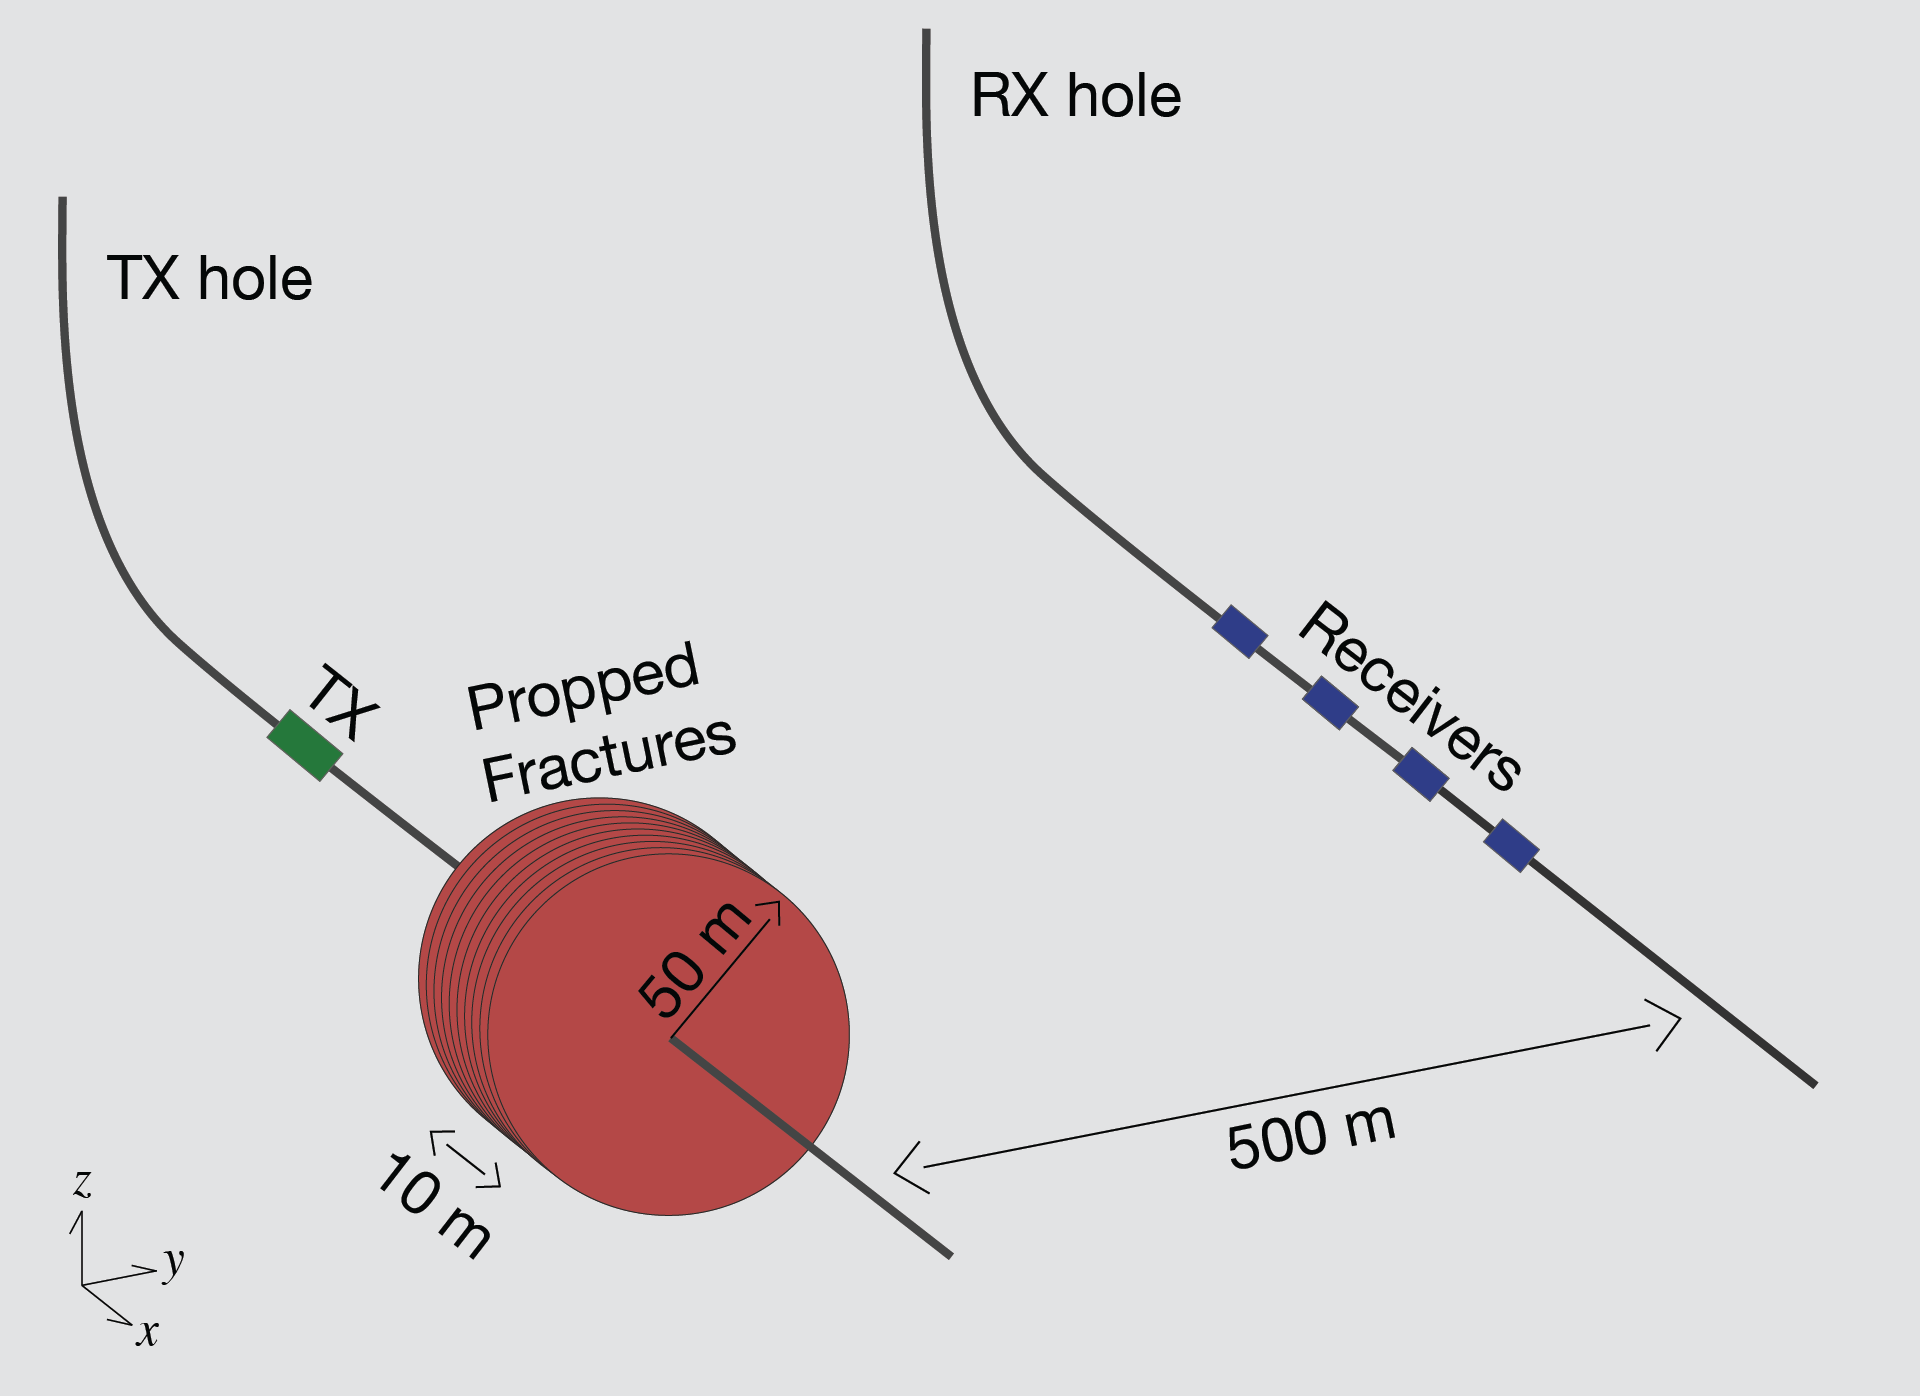
\includegraphics[width=\textwidth]{figures/phys_prop_model/crosswell_fractures.png}
    \end{center}
\caption{
    Setup for the crosswell electromagnetic simulation. Ten fractures, each with 3mm thickness
    and 50m radius are spaced over a 10m interval along the injection well. The dipole transmitter
    is positioned inside of the injection well and oriented along the x-axis. Receivers are located
    in an offset well and measure the real and imaginary parts of the x-component of the magnetic field.
}
\label{fig:crosswell_fractures}
\end{figure}


For the physical properties, I treat the background as a whole-space with a conductivity of 0.1 S/m. Within the fractures, I use a two-phase proppant-fluid mixture, where all of the proppant is assumed to be spherical particles as in Figure \ref{fig:emt_spherical_particles}. I use a proppant conductivity of $10^4$ S/m and a fluid conductivity of 3 S/m; in a 50-50 mixture, the effective conductivity computed using SCEMT, is 2500 S/m. To estimate the effective conductivity of the fractured volume of rock, I consider two scenarios: (1) the fractures are preferentially aligned and I estimate an anisotropic effective conductivity as in Figure \ref{fig:aligned_fractures}; and (2) the fractures are sufficiently complex that I can approximate them as a collection of randomly oriented cracks, as in Figure \ref{fig:random_fractures}. I estimate a single conductivity for the 10m wide cylinder with 50m radius that encloses the fractures. Within this region, the fractures comprise 0.3\% of the total volume. To estimate the aspect ratio, I assume that the shape of the large fracture, with 3mm width and 50m radius (100m diameter) is representative of the shape of the cracks that comprise it, thus the aspect ratio is $3\times10^{-5}$. The estimated effective conductivity for the anisotropic case is $\sigma_y = \sigma_z = 5$ S/m parallel to the fractures and $\sigma_x = 0.1$ S/m perpendicular to the fractures. For the second scenario, with randomly oriented cracks, the estimated isotropic conductivity is 3 S/m.

In terms of survey parameters, the dipole-moment of the transmitter is 5000 Am$^2$ and I use a transmitter frequency of 100Hz, consistent with values stated in \cite{Wilt1995, Wilt2003}. For a signal to be detectable, we require that: (a) the secondary signal, that is, the difference between the data measured with and without the fractures present, be above the noise floor of the receivers, and (b) that the secondary signal comprises a significant percentage of the primary (model without the fractures). \cite{Marsala2015a} demonstrated noise levels of $0.5 \times 10^-5$ nT and 0.5\% repeatability between data profiles for a cross-well survey conducted between two open-hole horizontal wells, citing that ``this was the lowest noise ever recorded with a crosswell EM system.'' Using this as an upper-bound on our expectations, I adopt a more conservative noise level of $1\times10^-4$ nT and select a percent-threshold of $5\%$. Thus, I consider signal above $1\times10^{-4}$ nT and comprising $>5\%$ of the primary as detectable.

Figure \ref{fig:crosswell_data100} shows the simulated secondary magnetic field data computed for (a) the anisotropic model and (b) the isotropic model at 100 Hz. The top row shows the real component and the bottom row shows the imaginary component. The x-axis shows the transmitter location relative to the center of the fracture, the y-axis shows the receiver location, and the color indicates the secondary magnetic field with respect to a 0.1 S/m whole-space. Regions of the plot which are colored, and are not covered by the semi-transparent overlay, indicate signal which is both above the noise floor and comprises a significant percentage of the primary.


\begin{figure}
    \begin{center}
    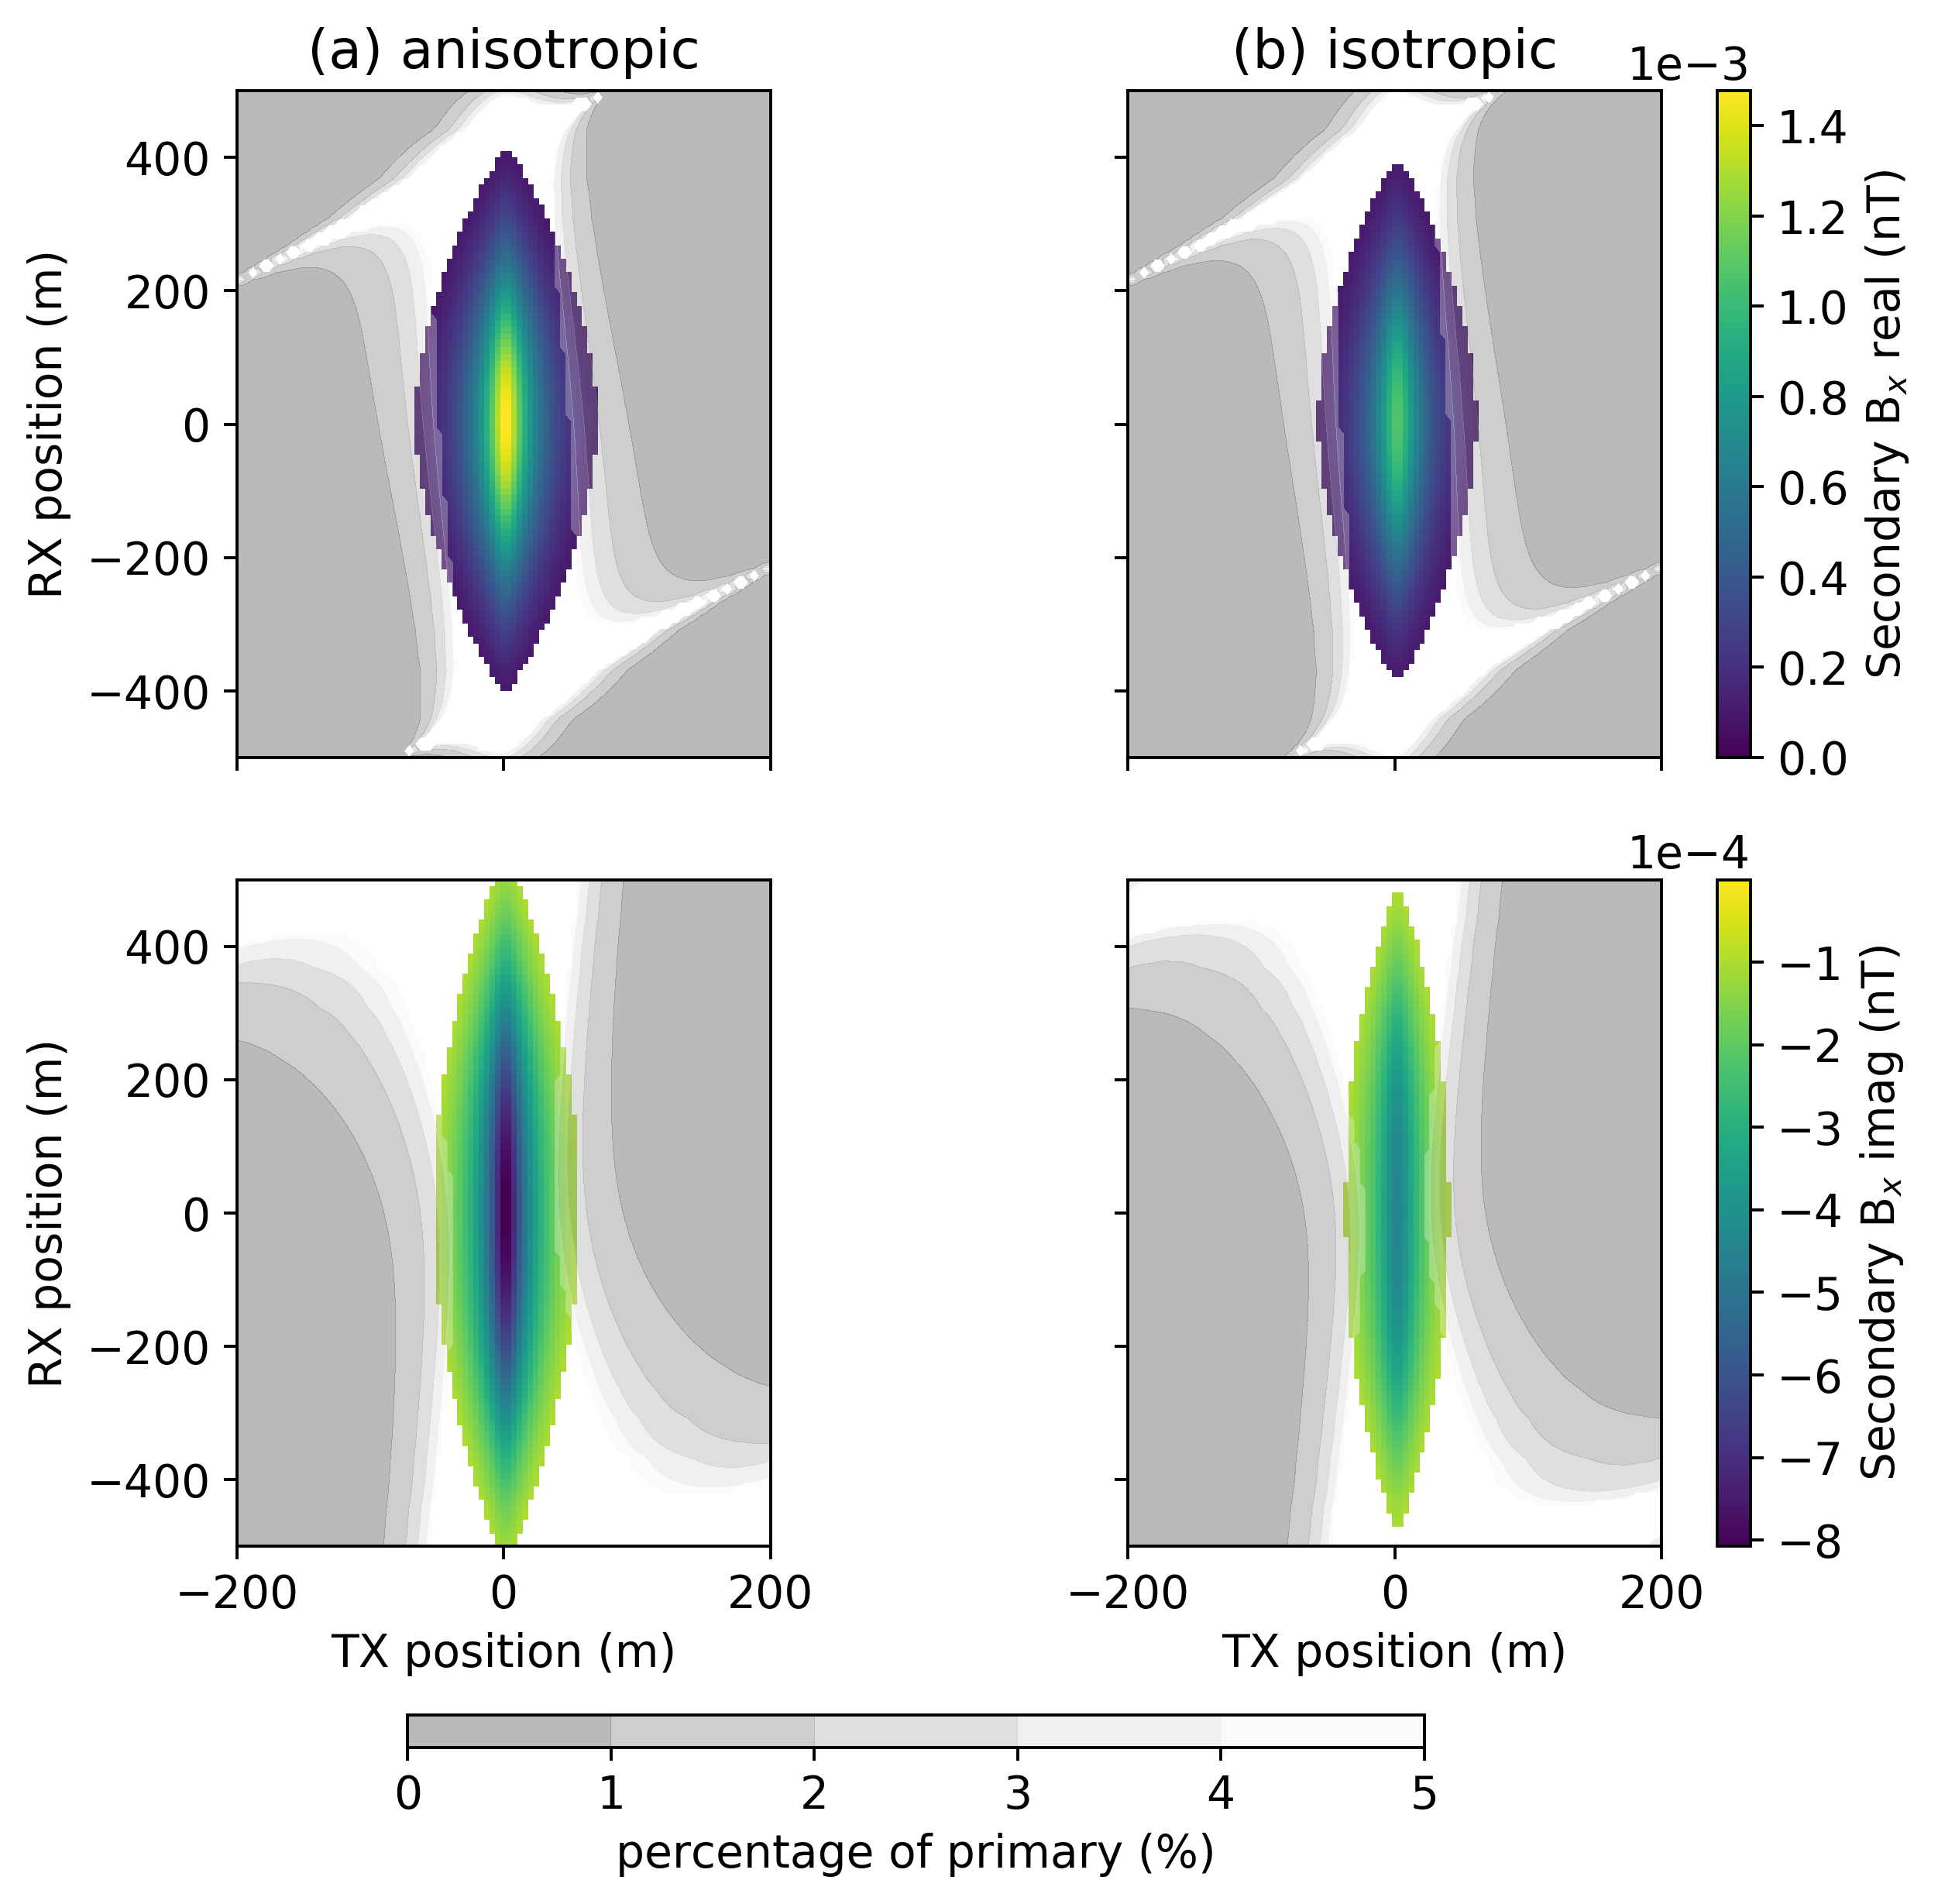
\includegraphics[width=\textwidth]{figures/phys_prop_model/crosswell_data100.png}
    \end{center}
\caption{
    Simulated secondary magnetic field data for: (a) the anisotropic fracture model and
    (b) the isotropic fracture model, in a crosswell survey conducted at 100Hz.
    The top row shows the real component and the bottom row shows
    the imaginary component of the measured magnetic flux (nT).
    In all plots, the x-axis shows the transmitter location relative to the center
    of the fracture, the y-axis shows the receiver location, and the color indicates the secondary
    magnetic flux with respect to a 0.1 S/m whole-space. Values beneath the noise floor of $10^{-4}$ nT
    have been masked and display as white. To display the signal as a percentage of the primary, we have
    included a semi-transparent overlay between 0\% and 5\%; low percentage values plot as darker
    greys.
}
\label{fig:crosswell_data100}
\end{figure}


As might be expected, when the transmitter and receiver are centered with the fracture, the secondary signal reaches its maximum amplitude in both the real and imaginary components. The anisotropic model produces stronger signals; the geometry of the survey is perfectly coupled to the radial components of the conductivity ($\sigma_y$ and $\sigma_z$) as the resultant currents and electric fields are purely azimuthal in orientation. An isotropic simulation using $\sigma = 5$ S/m produces identical results to the anisotropic model for this survey geometry. Interestingly, the region over which data is measurable differs between the real and imaginary components. The real component is measurable over a larger range of transmitter positions, while the imaginary component is measurable over a larger range of receiver locations. The partition of EM energy into the real and imaginary components is a function of the conductivity of the medium as well as the frequency. For example, if I increase the frequency to 200 Hz, the amplitude of the imaginary component is larger than the real, and it is measurable over a larger set of source-receiver combinations, as shown in Figure \ref{fig:crosswell_data200}.

\begin{figure}
    \begin{center}
    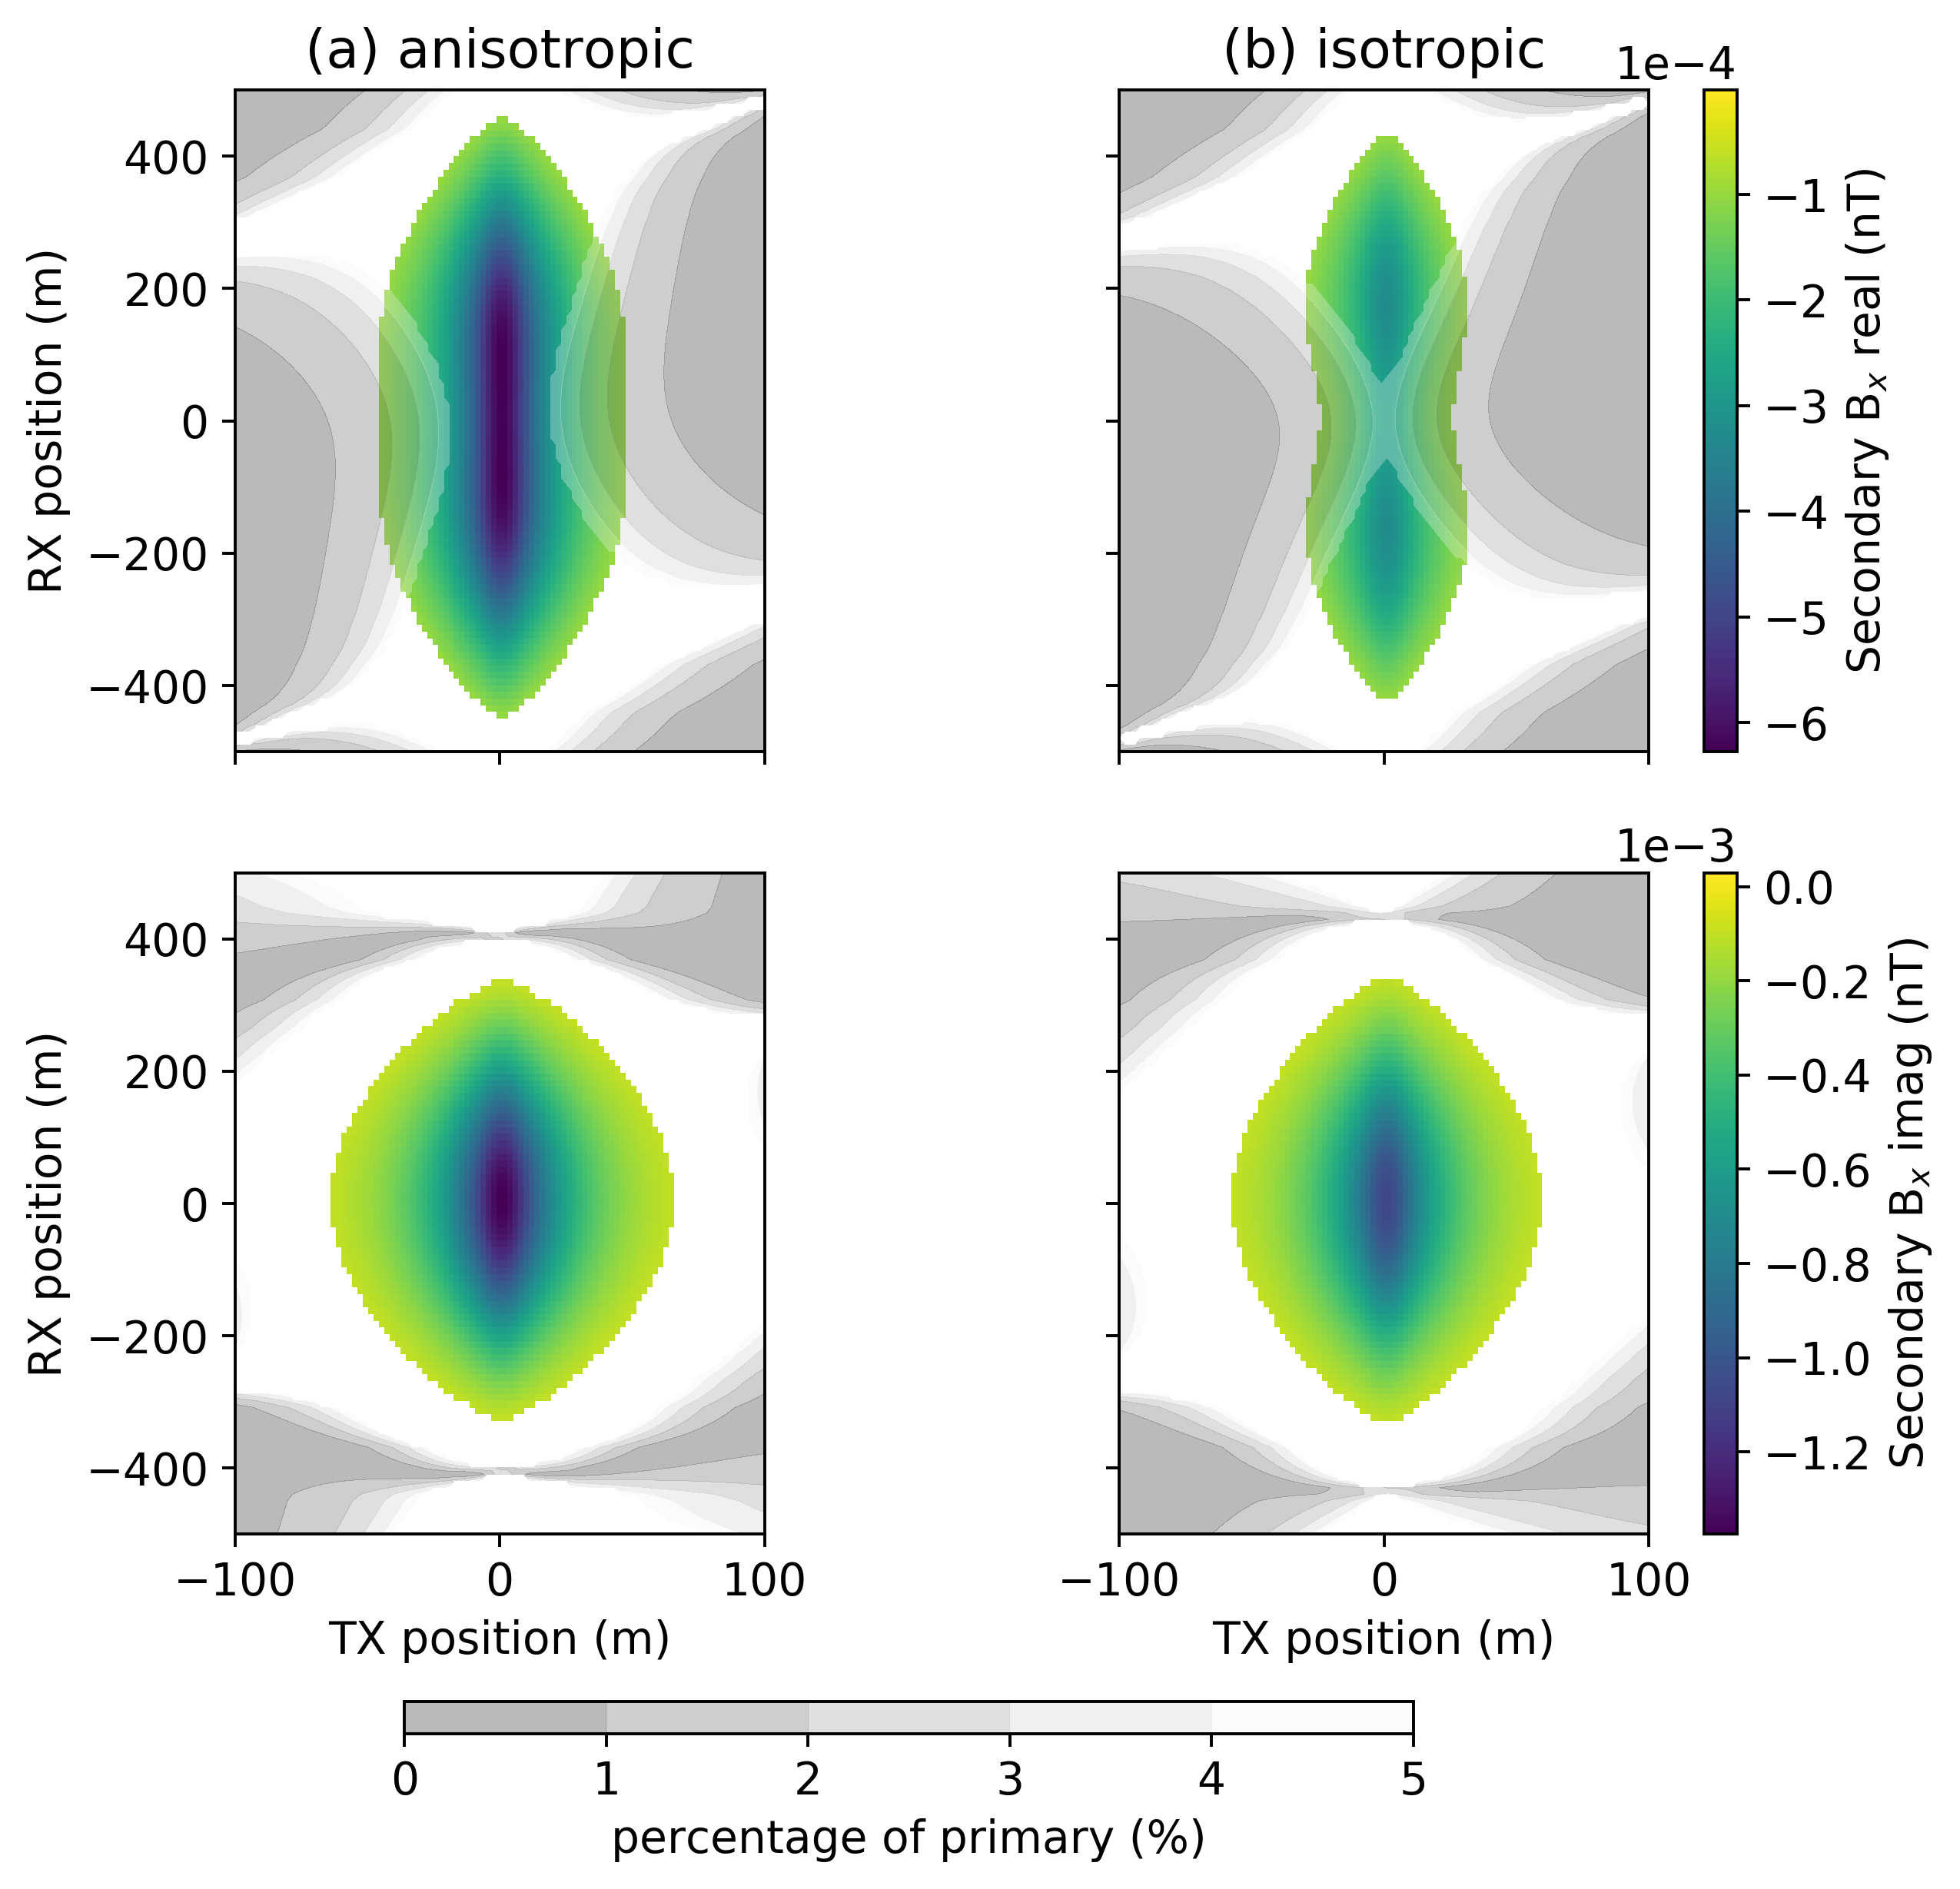
\includegraphics[width=\textwidth]{figures/phys_prop_model/crosswell_data200.png}
    \end{center}
\caption{
    Simulated secondary magnetic field data for: (a) the anisotropic fracture model and
    (b) the isotropic fracture model, in a crosswell survey conducted at 200Hz.
    The top row shows the real component and the bottom row shows
    the imaginary component of the measured magnetic flux (nT), similar to Figure \ref{fig:crosswell_data100}
}
\label{fig:crosswell_data200}
\end{figure}


For the simple setup shown here, there are a significant number of data that can be collected in a cross-well survey which are sensitive to both the anisotropic and isotropic fracture models. In both the 100 Hz and 200 Hz surveys, the extent over which either or both of the real and imaginary components of the data are above the noise floor and comprise a significant percentage of the primary field spanned ~100m for the transmitter location and $> 800$m for the receiver locations. These results provide confidence that EM is a potentially diagnostic tool for characterizing the propped region of a reservoir. Naturally, the success, or not, of EM in a given setting will depend upon the background conductivity, volume and conductivity of the proppant and fluid, as well as noise conditions in the field. Thus, forward modelling tailored to the setting is required to assess feasibility.
\section{Conclusion}

The large range of scales involved in describing a propped, fractured volume of rock as a geophysical target for an electromagnetic survey poses a challenge for performing numerical simulations. I approached this problem by using effective medium theory to estimate the electrical conductivity of a fracture volume of rock in two steps. First, I estimated the conductivity of a slurry containing proppant and fluid. I demonstrated several approaches for creating an electrically conductive slurry, including using conductive particles (or particles coated with a conductive material) as the proppant or including conductive particles, which might be elongated to enhance the conductivity at lower concentrations. General agreement with the values published in the laboratory experiment by \cite{Zhang2016} gives confidence that the estimates produced using effective medium theory are representative of the conductivities that can be achieved; a more rigorous comparison would require control on the conductivity of each of the constituents. In the second step, I estimated the effective conductivity of a fractured volume of rock by assuming that the fracture is composed of a collection of ellipsoidal cracks. These cracks may be preferentially oriented, if simple planar fractures are expected, or randomly oriented if a more complex fracture network is anticipated.

Using this approach, I developed isotropic and anisotropic electrical conductivity models considering proppant and fluid volumes that are representative of current hydraulic fracture operations and simulated a crosswell EM survey. In this example, the fractured volume was detectable if I assume noise estimates that have demonstrated to be achievable in horizontal wells for a waterflood monitoring experiment. This provides evidence that EM has the potential to be a suitable method for characterizing the propped region of a hydraulically fractured reservoir.

The examples examined here neglect the effects of steel-cased well on EM signals. In the vast majority of settings where hydraulic fracturing is conducted, the wells are cased with steel, and therefore, this complication  needs to be addressed. For induction problems, the concern is attenuation of the electromagnetic signals, as eddy currents may be induced in the steel cased well. However, there is increasing interest in using the steel casing as an ``extended electrode'' to help deliver current to depth. In the following chapters, I develop a strategy for including steel cased wells in the EM numerical simulations and examine their influence on EM signals.


%% The following is a directive for TeXShop to indicate the main file
%%!TEX root = ../../thesis.tex

\chapter{Modelling electromagnetics on cylindrical meshes}
\label{ch:casing-software}

A number of geophysical electromagnetic (EM) problems lend themselves to cylindrical geometries. Airborne EM problems over a 1D layered earth or borehole-logging applications fall into this category; in these cases cylindrical modelling, which removes a degree of freedom in the azimuthal component, can be advantageous as it reduces the computation load. This is useful when running an inversion where many forward modellings are required, and it  is also valuable when exploring and building up an understanding of the behaviour of electromagnetic fields and fluxes in a variety of settings, such as the canonical model of an airborne EM sounding over a sphere, as it reduces feedback time between asking a question and visualizing results (e.g. \cite{Oldenburg2017}).

Beyond these simple settings, there are also a range of scenarios where the footprint of the survey is primarily cylindrical, but 2D or 3D variations in the physical property model may be present. For example if we consider a single sounding in an Airborne EM survey, the primary electric fields are rotational and the magnetic fields are poloidal, but the physical property model may have lateral variations or compact targets. More flexibility is required from the discretization to capture these features. In this case, a 3D cylindrical geometry, which incorporates azimuthal discretization may be advantageous. It allows finer discretization near the source where we have the most sensitivity and the fields are changing rapidly. Far from the source, the discretization is coarser, but it still conforms to the primary behaviour of the EM fields and fluxes and captures the rotational electric fields and poloidal magnetic flux.

In other cases, the most significant physical property variations may conform to a cylindrical geometry, for example in settings where vertical metallic well-casings are present, or in the emerging topic of using geophysics to ``look ahead'' of a tunnel boring machine. Of particular interest to the thesis is understanding the behavior of electromagnetic fields and fluxes in the presence of steel-cased wells. In addition to the hydraulic fracturing application, understanding EM in settings with steel-cased wells is of interest across a range of applications, from characterizing lithologic units with well-logs \citep{Kaufman1990, Kaufman1993, Augustin1989}, to identifying marine hydrocarbon targets \citep{Kong2009, Swidinsky2013, Tietze2015}, to mapping changes in a reservoir induced by hydraulic fracturing or carbon capture and storage \citep{Pardo2013, Borner2015, Um2015, Weiss2016, hoversten2017borehole, Zhang2018}. Carbon steel, a material commonly used for borehole casings, is highly electrically conductive ($10^6 - 10^7$ S/m) and has a significant magnetic permeability ($\geq 100$ $\mu_0$) \citep{wuhabashy1994}; it therefore can have a significant influence on electromagnetic signals. The large contrasts in physical properties between the casing and the geologic features of interest, along with the large range of scales that need to be considered to model both the millimeter-thick casing walls while also capturing geologic features, provide interesting challenges and context for electromagnetics in cylindrical geometries.

In this chapter, I introduce an approach and associated open-source software implementation for simulating Maxwell's equations over conductive, permeable models on 2D and 3D cylindrical meshes. The software is written in Python \citep{van1995python} and is included as an extension to the SimPEG ecosystem \citep{Cockett2015}; Appendix \ref{app:simpegem} provides a description of the SimPEG electromagnetic module. Within the context of current research connected to steel-cased wells, my aim with the development and distribution of this software is two-fold: (1) to facilitate the exploration of the physics of EM in these large-contrast settings, and (2) to provide a simulation tool that can be used for testing other EM codes. The large physical property contrasts in both conductivity and permeability means the physics is complicated and often non-intuitive; as such, we prioritize the ability of the researcher to access and visualize fields, fluxes, and charges in the simulation domain. This is particularly useful when the software is used in conjunction with Jupyter notebooks which facilitate exploration of numerical results \citep{Perez2015}. As the mesh conforms to the geometry of a vertical borehole, a fine discretization can be used in its vicinity without resulting in a onerous computation. This provides the opportunity to build an understanding of the physics of EM in settings with vertical boreholes prior to moving to settings with deviated and horizontal wells. I demonstrate the software with examples at DC, in the frequency domain, and in the time domain. Source-code for all examples is provided as Jupyter notebooks as outlined in Appendix \ref{app:code_list}; they are licensed under the permissive MIT license with the hope of reducing the effort necessary by a researcher to compare to or build upon this work.

This chapter is organized in the following manner. In section \ref{sec:numerical_tools}, I introduce the governing equations, Maxwell's equations, and describe their discretization in cylindrical coordinates. I then compare our numerical implementation to the finite element and finite difference results shown in \citep{Commer2015} as well as a finite volume OcTree simulation described in \citep{Haber2007}. Section \ref{sec:numerical_examples} contains numerical examples of the DC, frequency domain EM, and time domain EM implementations. The two DC resistivity examples (sections \ref{sec:dc_resistivity_part1} and \ref{sec:dc_resistivity_part2}) are built upon the foundational work in \citep{Kaufman1990, Kaufman1993} which use asymptotic analysis to draw conclusions about the behavior of the electric fields, currents, and charges for a well where an electrode has been positioned along its axis.  The final two examples, in sections \ref{sec:FDEM_part1} and \ref{sec:FDEM_part2}, consider a frequency domain experiment inspired by \citep{Augustin1989}. These examples demonstrate the impact of magnetic permeability on the character of the magnetic flux within the vicinity of the borehole and discusses the resulting magnetic field measurements made within a borehole.
\section{Numerical tools}
\label{sec:numerical_tools}

The governing equations under consideration are Maxwell's equations. I provided an overview in Section \ref{sec:background-em}. This section is meant to provide a brief review and set the context for what is required of our numerical tools.

Under the quasi-static approximation, Maxwell's equations are given by:
\begin{equation}
\begin{split}
\nabla \times \vec{e} &= -\frac{\partial \vec{b}}{\partial t} \\
\nabla \times \vec{h} - \vec{j} &= \vec{s}_e
\end{split}
\label{eq:MaxwellTime}
\end{equation}

where $\vec{e}$ is the electric field, $\vec{b}$ is the magnetic flux density, $\vec{h}$ is the magnetic field, $\vec{j}$ is the current density and $\vec{s_e}$ is the source current density. Maxwell's equations can also be formulated in the frequency domain, using the $e^{i \omega t}$ Fourier Transform convention, they are
\begin{equation}
\begin{split}
\nabla \times \vec{E} + i\omega\vec{B} &= 0 \\
\nabla \times \vec{H} - \vec{J} &= \vec{S}_e
\end{split}
\label{eq:MaxwellFreq}
\end{equation}

The fields and fluxes are related through the physical properties: electrical conductivity ($\sigma$, or its inverse, resistivity $\rho$) and magnetic permeability ($\mu$), as described by the constitutive relations
\begin{equation}
\begin{split}
\vec{J} = \sigma \vec{E} \\
\vec{B} = \mu \vec{H}
\end{split}
\label{eq:ConstitutiveRelations}
\end{equation}

At the zero-frequency limit, we also consider the DC resistivity experiment, described by
\begin{equation}
\begin{split}
\nabla \cdot \vec{j} &= I\left(\delta(\vec{r} - \vec{r}_{s^{+}}) - \delta(\vec{r} - \vec{r}_{s^{-}})\right) \\
\vec{e} &= - \nabla \phi
\end{split}
\label{eq:DCequations}
\end{equation}

where $I$ is the magnitude of the source current density, $\vec{r}_{s^+}$ and $\vec{r}_{s^-}$ are the locations of the current electrodes, and $\phi$ is the scalar electric potential.

Of our numerical tools, we require the ability to simulate large electrical conductivity contrasts, include magnetic permeability, and solve Maxwell's equations at DC, in frequency and in time in a computationally tractable manner. Finite volume methods are advantageous for modelling large physical property contrasts as they are conservative and the operators ``mimic'' properties of the continuous operators, that is, the edge curl operator is in the null space of the face divergence operator, and the nodal gradient operator is in the null space of the edge curl operator \citep{Hyman1999}. As such, they are common practice for many electromagnetic simulations (e.g. \cite{Horesh2011, Haber2014, Jahandari2014} and references within), and will be my method of choice.
\subsection{Discretization}
To represent a set of partial differential equations on the mesh, I use a staggered-grid approach \citep{Yee1966} and discretize fields on edges, fluxes on faces, and physical properties at cell centers, as shown in Figure \ref{fig:CylFiniteVolume}. Scalar potentials can be discretized at cell centers or nodes. I consider both cylindrically symmetric meshes and fully 3D cylindrical meshes; the anatomy of a finite volume cell for these scenarios is shown in Figure \ref{fig:CylFiniteVolume} (b) and (c).


\begin{figure}
    \begin{center}
    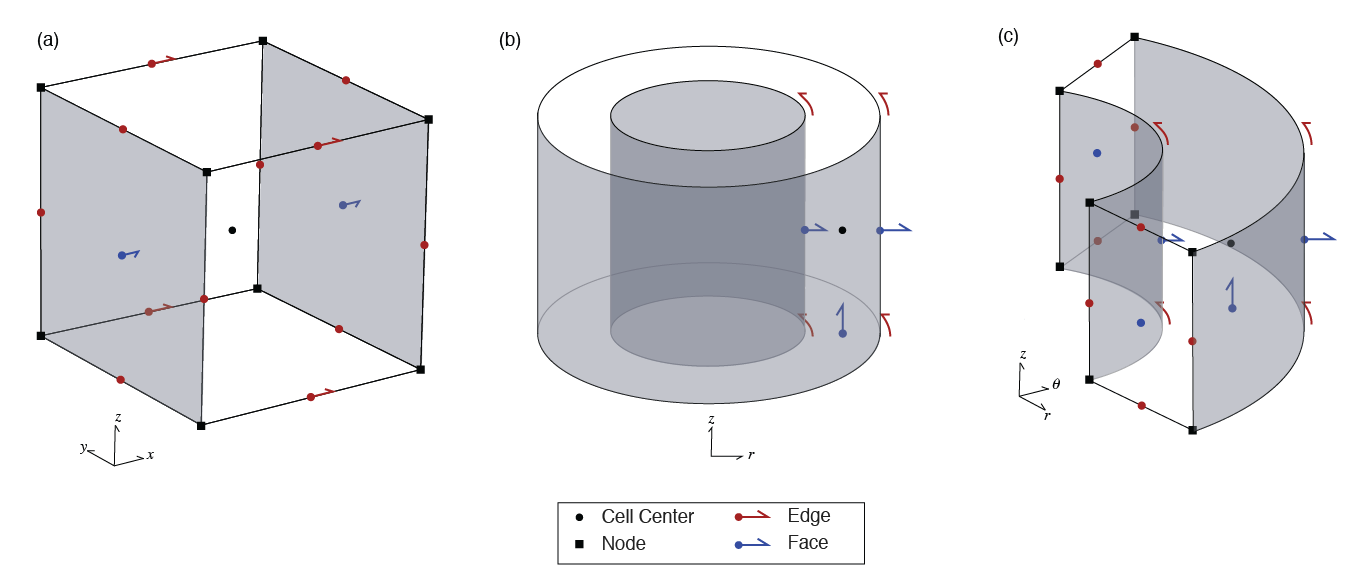
\includegraphics[width=\columnwidth]{figures/casing_software/finiteVolume-02.png}
    \end{center}
\caption{
    Anatomy of a finite volume cell in a (a) cartesian,
    regtangular mesh, (b) cylindrically symmetric mesh, and
    (c) a three dimensional cylindrical mesh.
}
\label{fig:CylFiniteVolume}
\end{figure}


To discretize Maxwell's equations in the time domain (equation \ref{eq:MaxwellTime}) or in the frequency domain (equation \ref{eq:MaxwellFreq}), I invoke the constitutive relations to formulate our system in terms of a single field and a single flux. This gives a system in either the electric field and magnetic flux (E-B formulation), or the magnetic field and the current density (H-J formulation). For example, in the frequency domain, the E-B formulation is
\begin{equation}
    \begin{split}
        \mathbf{C} \mathbf{e} + i\omega\mathbf{b} &= \mathbf{s_m} \\
        \mathbf{C}^\top \mathbf{M}_{\boldsymbol{\mu}^{-1}}^f \mathbf{b} - \mathbf{M}_{\boldsymbol{\sigma}}^e \mathbf{e} &= \mathbf{s_e}
    \end{split}
    \label{eq:DiscreteFDEMEB}
\end{equation}

and the H-J formulation is
\begin{equation}
    \begin{split}
        \mathbf{C}^\top \mathbf{M}_{\boldsymbol{\rho}}^f \mathbf{j} + i\omega\mathbf{M}_{\boldsymbol{\mu}}^e\mathbf{h} &= \mathbf{0} \\
        \mathbf{C} \mathbf{h} - \mathbf{j} &= \mathbf{s_e}
    \end{split}
    \label{eq:DiscreteFDEMHJ}
\end{equation}

where $\mathbf{e}, \mathbf{b}, \mathbf{h}, \mathbf{j}$ are vectors of the discrete EM fields and fluxes; $\mathbf{s_m}$ and $\mathbf{s_e}$ are the discrete magnetic and electric source terms, respectively; $\mathbf{C}$ is the edge curl operator, and the matrices $\mathbf{M}_{\text{prop}}^{e,f}$ are the edge / face inner product matrices. In particular, variable electrical conductivity and variable magnetic permeability are captured in the discretization. The time domain equations are discretized in the same manner; for time-stepping, a first-order backward Euler approach is used. Although the midpoint method, which is second-order accurate, could be considered, it is susceptible to oscillations in the solution, which reduce the order of accuracy, unless a sufficiently small time-step is used \citep{Haber2004, Haber2014}.  Appendix \ref{app:simpegem} provides more details on the discretization of Maxwell's equations in both the frequency and time-domains.

At the zero-frequency limit, each formulation has a complementary discretization for the DC equations. For the E-B formulation the discretization leads to a nodal discretization of the electric potential $\boldsymbol{\phi}$, giving
% \begin{equation}
%     \mathbf{G}^\top \mathbf{M}_{\boldsymbol{\sigma}}^e \mathbf{G} \boldsymbol{\phi} = \mathbf{q}
%     \label{eq:DiscreteDCNodal}
% \end{equation}
\begin{equation}
    \begin{split}
        - \mathbf{G}^\top \mathbf{M}_{\boldsymbol{\sigma}}^e \mathbf{e} &= \mathbf{q} \\
        \mathbf{e} &= -\mathbf{G}\boldsymbol{\phi}
    \end{split}
    \label{eq:DiscreteDCNodal}
\end{equation}

where $\mathbf{G}$ is the nodal gradient operator, and $\mathbf{q}$ is the source term, defined on nodes. Note that the nodal gradient takes the discrete derivative of nodal variables, and thus the output is on edges. The H-J formulation leads naturally to a cell centered discretization of the electric potential
\begin{equation}
    \begin{split}
        \mathbf{V} \mathbf{D}  \mathbf{j} &= \mathbf{q} \\
        \mathbf{M}_{\boldsymbol{\rho}}^f \mathbf{j} &= \mathbf{D}^\top \mathbf{V} \boldsymbol{\phi}
    \end{split}
    \label{eq:DiscreteDCCC}
\end{equation}

Where $\mathbf{D}$ is the face divergence operator, $\mathbf{V}$ is a diagonal matrix of the cell volumes, $\mathbf{q}$ is the source term, which is  defined at cell centers as is $\boldsymbol{\phi}$. Here, the face divergence takes the discrete derivative from faces to cell centers, thus its transpose takes a variable from cell centers to faces. For a tutorial on the finite volume discretization of the DC equations, see \citep{Cockett2016}.

For the EM simulations, natural boundary conditions are employed; in the E-B formulation, this means $\vec{B}\times\vec{n} = 0\vert_{\partial \Omega}$, and in the H-J formulation, we use $\vec{J}\times\vec{n} = 0\vert_{\partial \Omega}$. Within the DC simulations, there is flexibility on the choice of boundary conditions employed. In the simplest scenario, for the nodal discretization, we use Neumann boundary conditions, $\sigma\vec{E} \cdot \vec{n} = 0\vert_{\partial \Omega}$, and for the cell centered discretization, we use Dirichlet boundary conditions $\phi = 0\vert_{\partial \Omega}$.

When employing a cylindrical mesh, the distinction between where the electric and magnetic contributions are discretized in each formulation has important implications. If we consider the cylindrically symmetric mesh (Figure \ref{fig:CylFiniteVolume}b) and a magnetic dipole source positioned along the axis of symmetry (sometimes referred to as the TE mode), we must use the E-B formulation of Maxwell's equation to simulate the resulting toroidal magnetic flux and rotational electric fields. If instead, a vertical current dipole is positioned along the axis of symmetry (also referred to as the TM mode), then the H-J formulation of Maxwell's equations must be used in order to simulate toroidal currents and rotational magnetic fields. The advantage of a fully 3D cylindrical mesh is that it provides additional degrees of freedom, with the discretization in the azimuthal direction. This allows us to simulate more complex responses. However, in order to avoid the need for very fine discretization in the azimuthal direction, we should select the most natural formulation of Maxwell's equations given the source geometry being considered. For a vertical steel cased well and a grounded source, we expect the majority of the currents to flow vertically and radially, thus the more natural discretization to employ is the H-J formulation of Maxwell's equations.

\cite{Haber2014} provides derivations and discussion of the differential operators and inner product matrices; though they are described for a cartesian coordinate system and a rectangular grid, the extension to a three dimensional cylindrical mesh is straightforward. Effectively, a cartesian mesh is wrapped so that the $x$ components become $r$ components, and $y$ components become $\theta$ components, as shown in Figure \ref{fig:cylwrap}.


\begin{figure}
    \begin{center}
    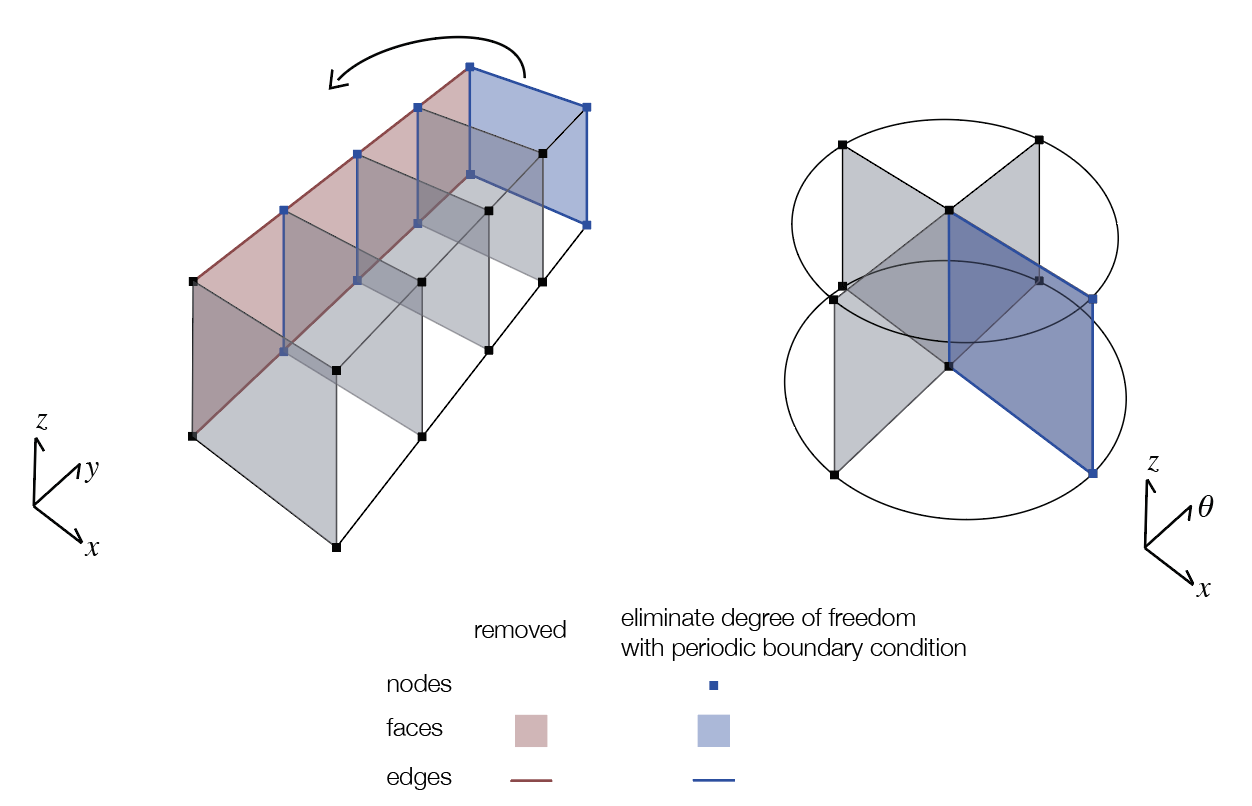
\includegraphics[width=0.9\columnwidth]{figures/cylwrap.png}
    \end{center}
\caption{Construction of a 3D cylindrical mesh from a cartesian mesh.}
\label{fig:cylwrap}
\end{figure}


The additional complications that are introduced are: (1) the periodic boundary condition introduced on boundary faces and edges in the azimuthal direction, (2) the removal of radial faces and azimuthal edges along the axis of symmetry, and (3) the elimination of the degrees of freedom of the nodes and edges at the boundary and as well as the nodes and vertical edges along the axis of symmetry. The implementation of the 3D cylindrical mesh is provided as a part of the \texttt{discretize} package (http://discretize.simpeg.xyz), which is an open-source python package that contains finite volume operators and utilities for a variety of mesh-types. All differential operators are tested for second order convergence and for preservation of mimetic properties (as described in \cite{Haber2014}). \texttt{discretize} is developed in a modular, object-oriented manner and interfaces to all of the SimPEG forward modelling and inversion routines, thus, once the differential operators have been implemented, they can be readily used to perform forward simulations \citep{Cockett2015}.  One of the benefits of SimPEG for forward simulations is that values of the fields and fluxes are readily computed and visualized, which enables researchers to examine the physics as well as to simulate data. Development within the SimPEG ecosystem follows best practices for modern, opens-source software, including: peer review of code changes and additions, versioning, automated testing, documentation, and issue tracking.

\subsection{Validation}
Testing for the DC, TDEM, and FDEM implementations includes comparison with analytic solutions for a dipole in a whole-space. These examples are included as supplementary examples with the distributed notebooks. I have also compared the cylindrically symmetric implementation at low frequency with a DC simulation from a Resistor Network solution developed in MATLAB with (Figure 3 in \cite{Yang2016}).

Here, I include a comparison with the time domain electromagnetic simulation shown in Figures 13 and 14 of \cite{Commer2015}. A 200m long well, with a conductivity of $10^{6}$ S/m, outer diameter of 135 mm, and casing thickness of 12 mm is embedded in a 0.0333 S/m background. For the material inside the casing, I use a conductivity equal to that of the background. The conductivity of the air is set to $3 \times 10^{-4}$ S/m and the permeability of the casing is ignored ($\mu = \mu_0$). A 10 m long inline electric dipole source is positioned on the surface, 50 m radially from the well. The radial electric field is sampled at 5 m, 10 m, 100 m, 200 m and 300 m along a line $180^{\circ}$ from the source.

Two simulations are included in \cite{Commer2015}: a finite element (FE) and a finite difference (FD) solution. Both simulation meshes capture the thickness of the casing with a single cell or single tetrahedral element. The finite element solution mesh consisted of over 8 million tetrahedral elements and the simulation completed in 63 hours on a single core of an Intel Xeon X5550 processor (2.67 GHz). For the finite difference solution, a conservative time-stepping was used ($\Delta t = 3 \times 10^{-10}$ s), resulting in a total of $>$120 million time steps. This simulation took 23.2 hours using 512 cores on an Intel Xeon architecture (2.33 GHz).

Additionally, I include a comparison with the 3D UBC finite volume OcTree time domain code \citep{Haber2007}. The OcTree mesh allows for adaptive refinement of the mesh around sources, receivers, and conductivity structures within the domain, thus reducing the number of unknowns in the domain as compared to a tensor mesh. The mesh in the UBC simulation included 5,011,924 cells, with the finest cells being equal to the width of the casing; 154 time steps were taken and 10 different step-lengths were used (requiring 10 different matrix factorizations). This simulation took 57 minutes to run on a single Intel Xeon X5660 processor (2.80GHz).

For the 3D cylindrical simulation, I use a mesh that has 4 cells radially across the width of the casing, 2.5 m vertical discretization, and azimuthal refinement near the source and receivers (along the $\theta=90^\circ$ line), as shown in Figure \ref{fig:commer_model}. The mesh has a total of 309 120 cells. For the time discretization, the smallest time-step I use is $10^{-6}$ s; the time-mesh is coarsened at later times. I used a moderately conservative time-stepping scheme with 187 time-steps total. Seven different step-lengths were employed, requiring seven matrix factorizations. To solve the system matrix, the direct solver PARDISO was used \citep{Petra2014, Cosmin2016}. The simulation took 14 minutes to run on a single Intel Xeon X5660 processor (2.80GHz).



\begin{figure}
    \begin{center}
    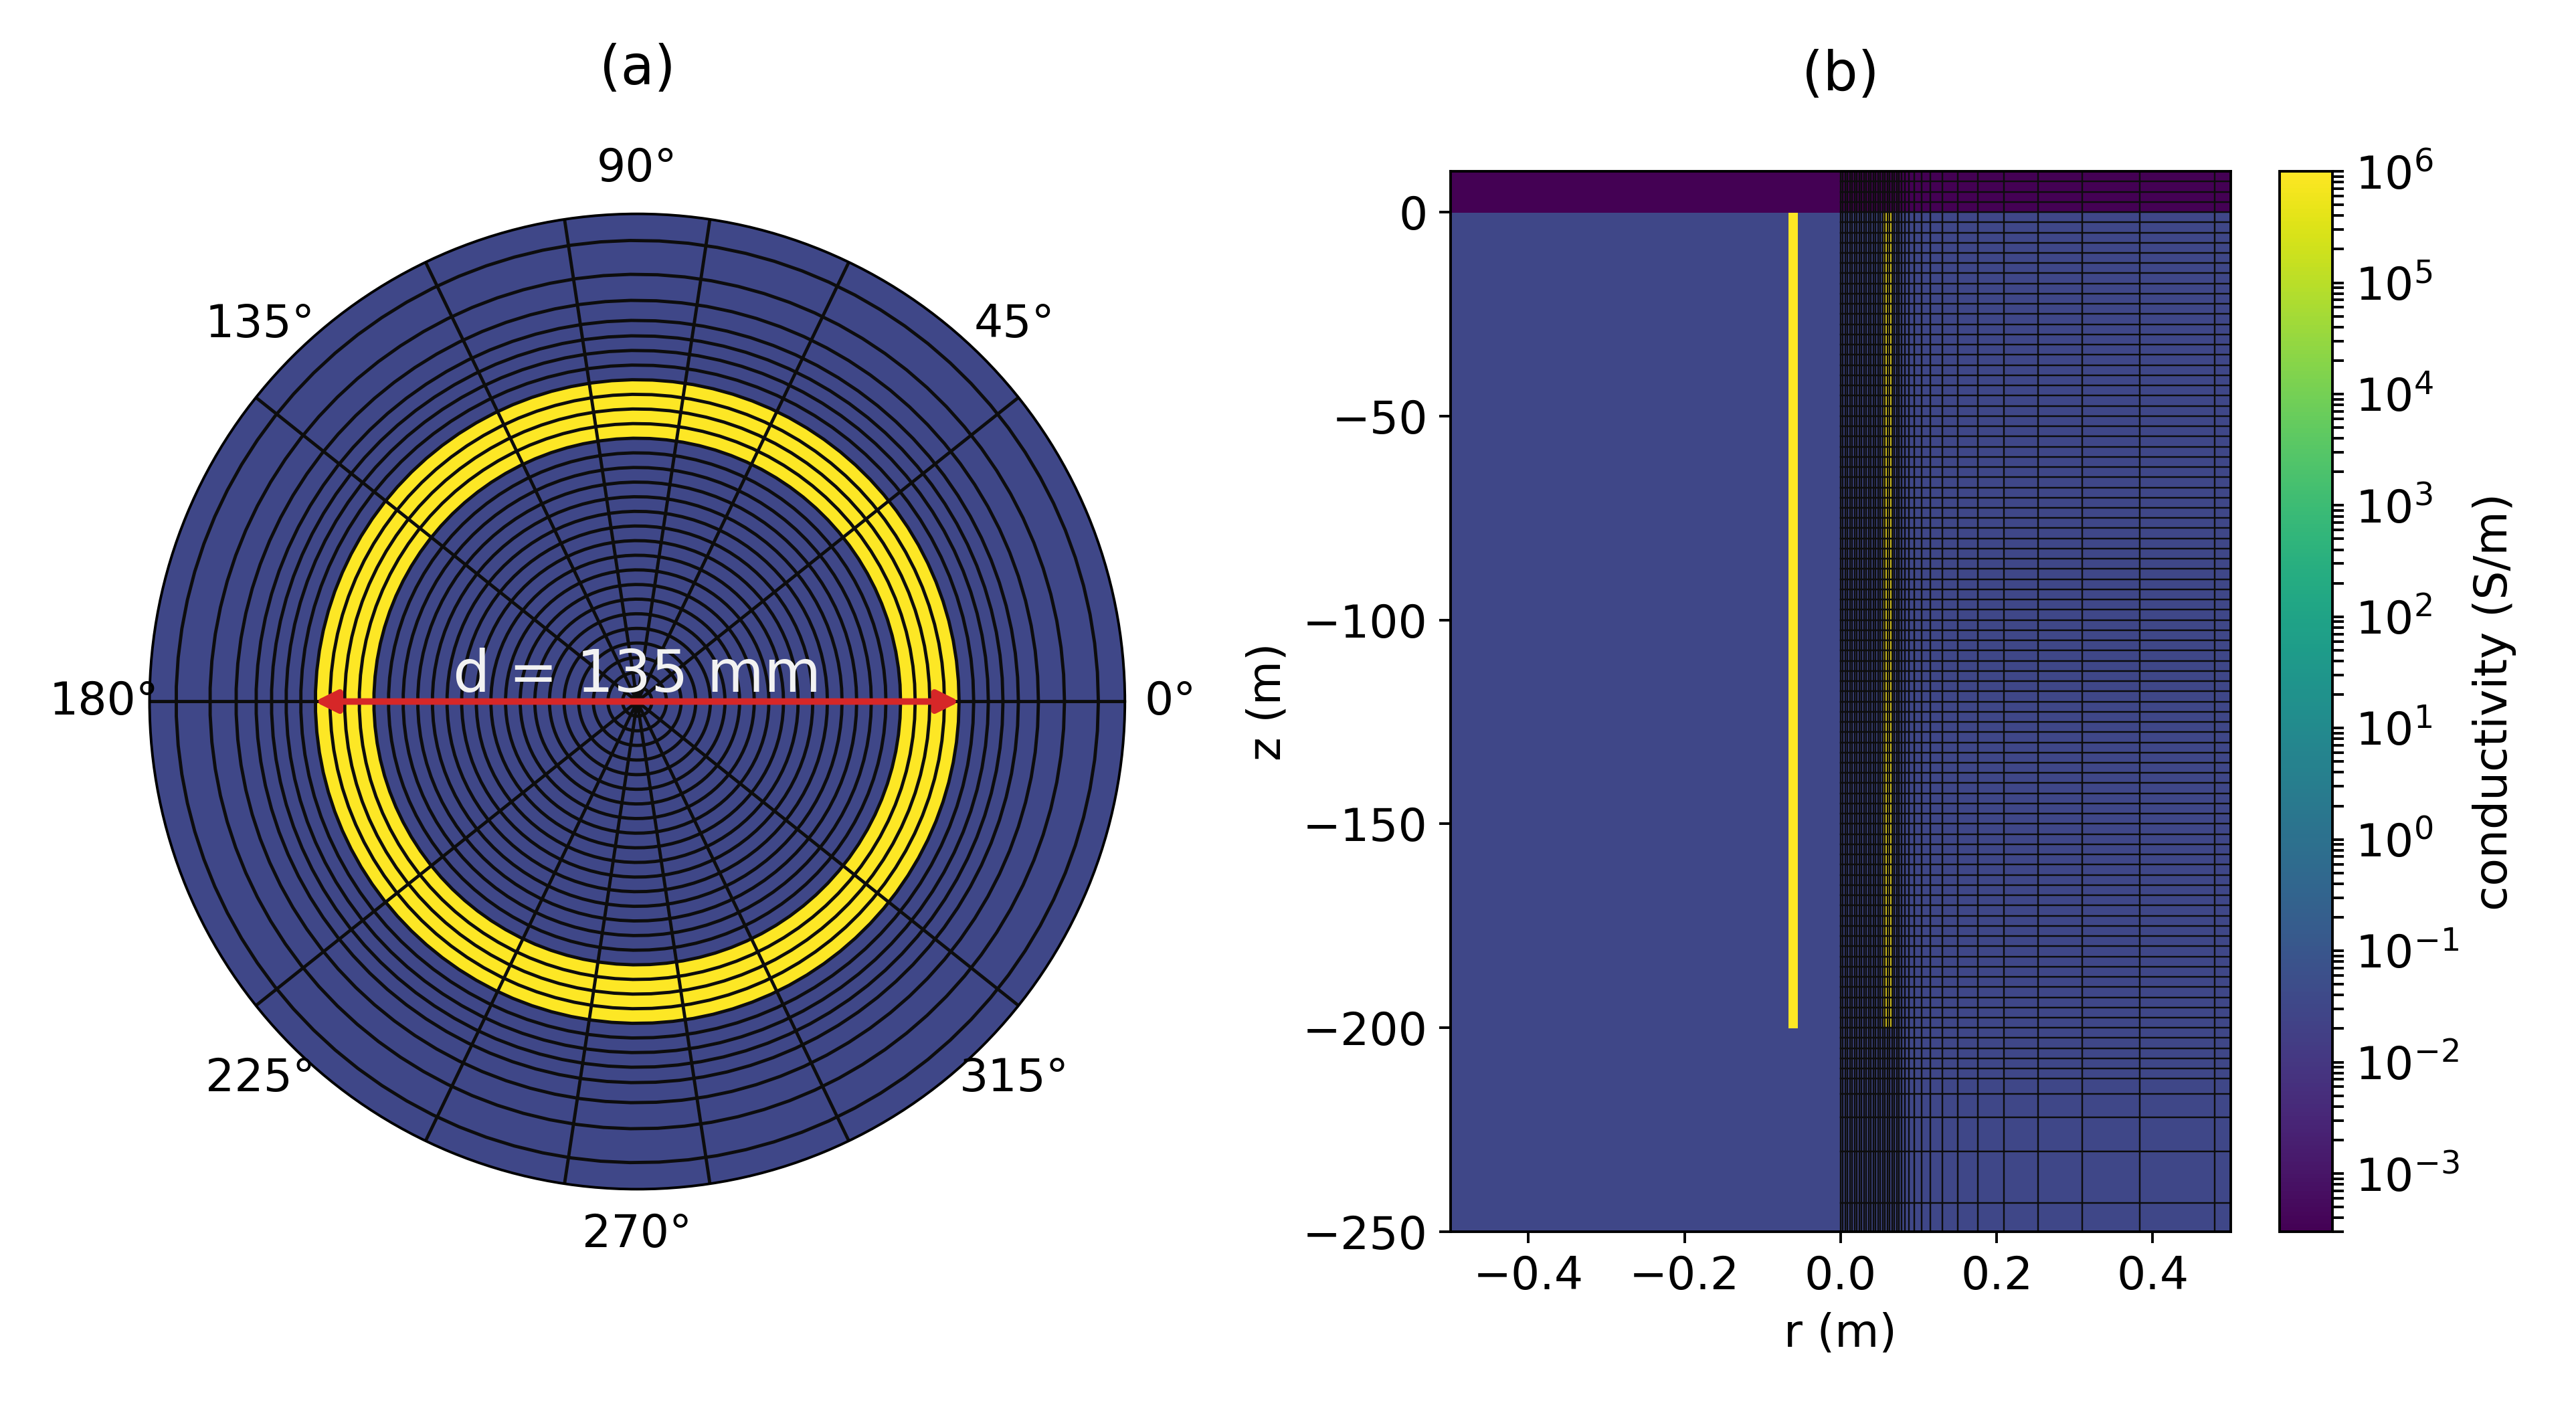
\includegraphics[width=0.8\columnwidth]{figures/casing_software/commer_model.png}
    \end{center}
\caption{
    Depth slice (left) and cross section (right) through the 3D cylindrical
    mesh used for the comparison with \cite{Commer2015}.
    The source and recievers are positioned along the $\theta = 90^\circ$ line.
    The mesh extends 17km raidally and 30km vertically to ensure that the fields
    have sufficiently decayed before reaching the boundaries.
}
\label{fig:commer_model}
\end{figure}



In Figure \ref{fig:commer_results}, I show the absolute value of the radial electric field sampled at five stations; each of the different line colors is associated with a different location, and offsets are with respect to the location of the well. Solutions were interpolated to the same offset using nearest neighbor interpolation.The 3D cylindrical simulation (SimPEG) is plotted with a solid line and overlaps with the UBC solution (dash-dot line) for all times shown. The finite element (FE) solution from \cite{Commer2015} is shown with the dashed lines, and the finite difference (FD) solution is plotted with dotted lines. The 3D cylindrical (SimPEG) and UBC solutions are overall in good agreement with the solutions from \cite{Commer2015}. There is a difference in amplitude and position of the zero-crossing (the v-shape visible in the blue and orange curves) between the Commer solutions and the SimPEG / UBC solutions at the shortest two offsets in the early times. At such short offsets from a highly conductive target, details of the simulation and discretization, such as the construction of the physical property matrices in each of the various approaches become significant; this likely accounts for the discrepancies but a detailed code-comparison is beyond the scope of this chapter. My aim with this comparison is to provide evidence that the numerical simulation is performing as expected; the overall agreement with Commer's and UBC's results is provides confidence that it is.


\begin{figure}[htb]
    \begin{center}
    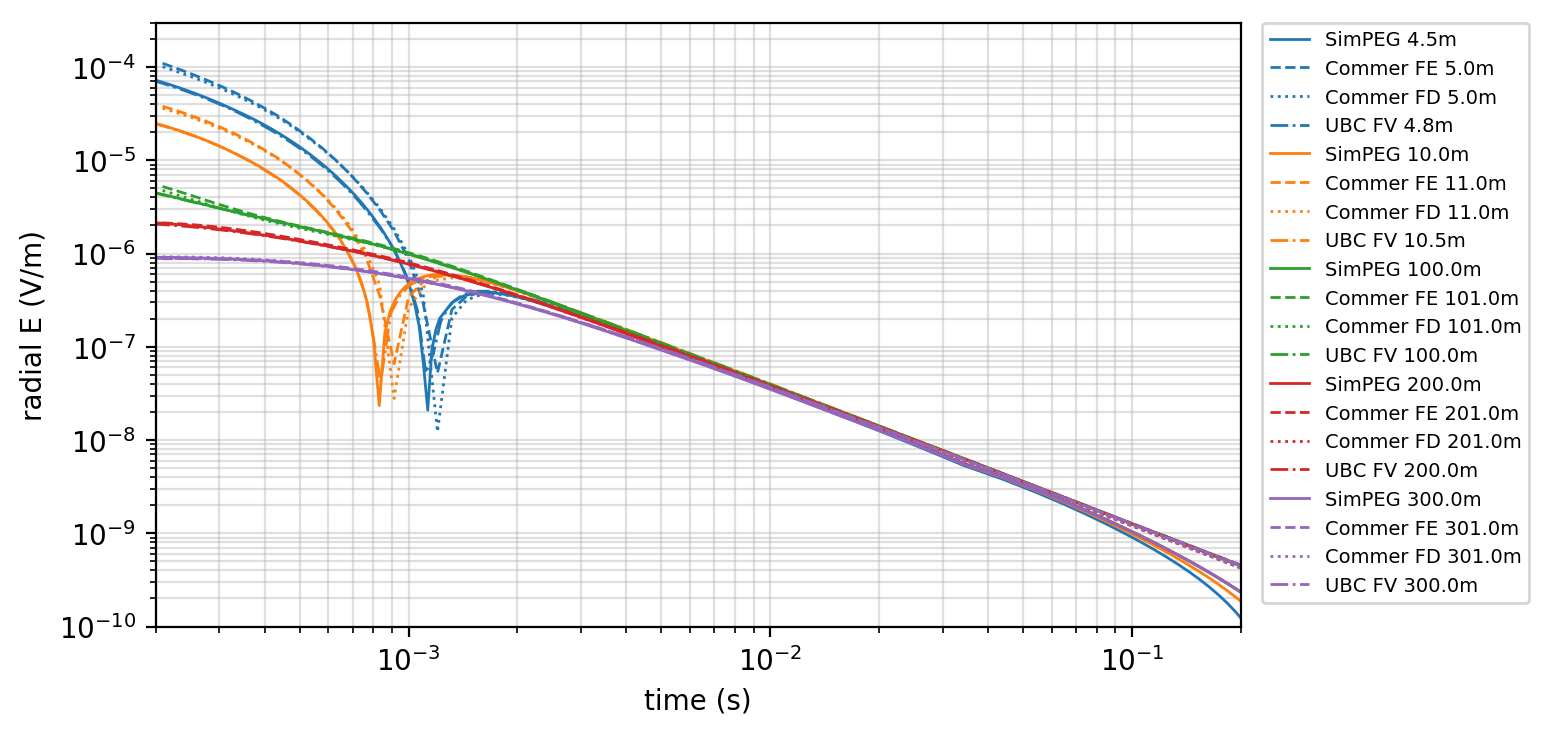
\includegraphics[width=\columnwidth]{figures/commer_results.png}
    \end{center}
\caption{Time domain EM response comparison with \citep{Commer2015}. Each of the different line colors is associated with a different location; offsets are with respect to the location of the well.}
\label{fig:commer_results}
\end{figure}


This example demonstrates agreement between the 3D cylindrical solution and solutions obtained with independently developed codes. Importantly, it also shows how, by using a cylindrical discretization which conforms to the conductivity structure of interest, the size of the mesh and resultant cost of the computation can be greatly reduced. This is true even with relatively conservative spatial and temporal discretizations. Minimizing computation time was not a main focus in the development of the software and there are still opportunities for improving efficiency. As an open-source project, contributions from the wider community are encouraged.
\section{Numerical Examples}
\label{sec:numerical_examples}

The numerical experiments I consider in this section are motivated by the need to use this software to delve into the physics of DC and EM in settings with steel cased wells. As such, the examples build upon examples in analytical derivations and asymptotic analyses in \cite{Kaufman1990, Kaufman1993} at DC and \cite{Augustin1989} for frequency domain EM. I do this to provide confidence that the physical phenomena we observe in the simulations are expected by theory as well as to build a foundation for discussion in the subsequent chapters.
\subsection{DC Resistivity Part 1: Electric fields, currents and charges in a long well}
\label{sec:dc_resistivity_part1}

In his two seminal papers on the topic, Kaufman uses transmission line theory to draw conclusions about the behaviour of the electric field when an electrode is positioned inside of an infinite casing. In this first example, I will revisit some of the physical insights discussed in \citep{Kaufman1990, Kaufman1993} that followed from an analytical derivation and compare those to my numerical results. In the second example, I look at the distribution of current and charges as the length of the well is varied and compare those to the analytical results discussed in \citep{Kaufman1993}

I start by considering a 1 km long well ($10^6$ S/m) in a whole space ($10^{-2}$ S/m), with the conductivity of the material inside the borehole equal to that of the whole space.  For modelling, I will use a cylindrically symmetric mesh. The positive electrode is positioned on the borehole axis in the mid-point of a 1 km long well;  a distant return electrode is positioned 1 km away at the same depth.

Kaufman discusses the behavior of the electric field by dividing the response into three zones: a near zone, an intermediate zone and a far zone \citep{Kaufman1990, Kaufman1993}. In the near zone, the electric field has both radial and vertical components, negative charges are present on the inside of the casing, and positive charges are present on the outside of the casing. The near zone is quite localized and typically, its vertical extent is no more than $\sim 10$ borehole radii away from the electrode. To examine these features in our numerical simulation, I have plotted in Figure \ref{fig:kaufman_zones}: (a)  the total charge, (b) secondary charges, (c) electric field, and (d) current density in a portion of the model near the source.


\begin{figure}
    \begin{center}
    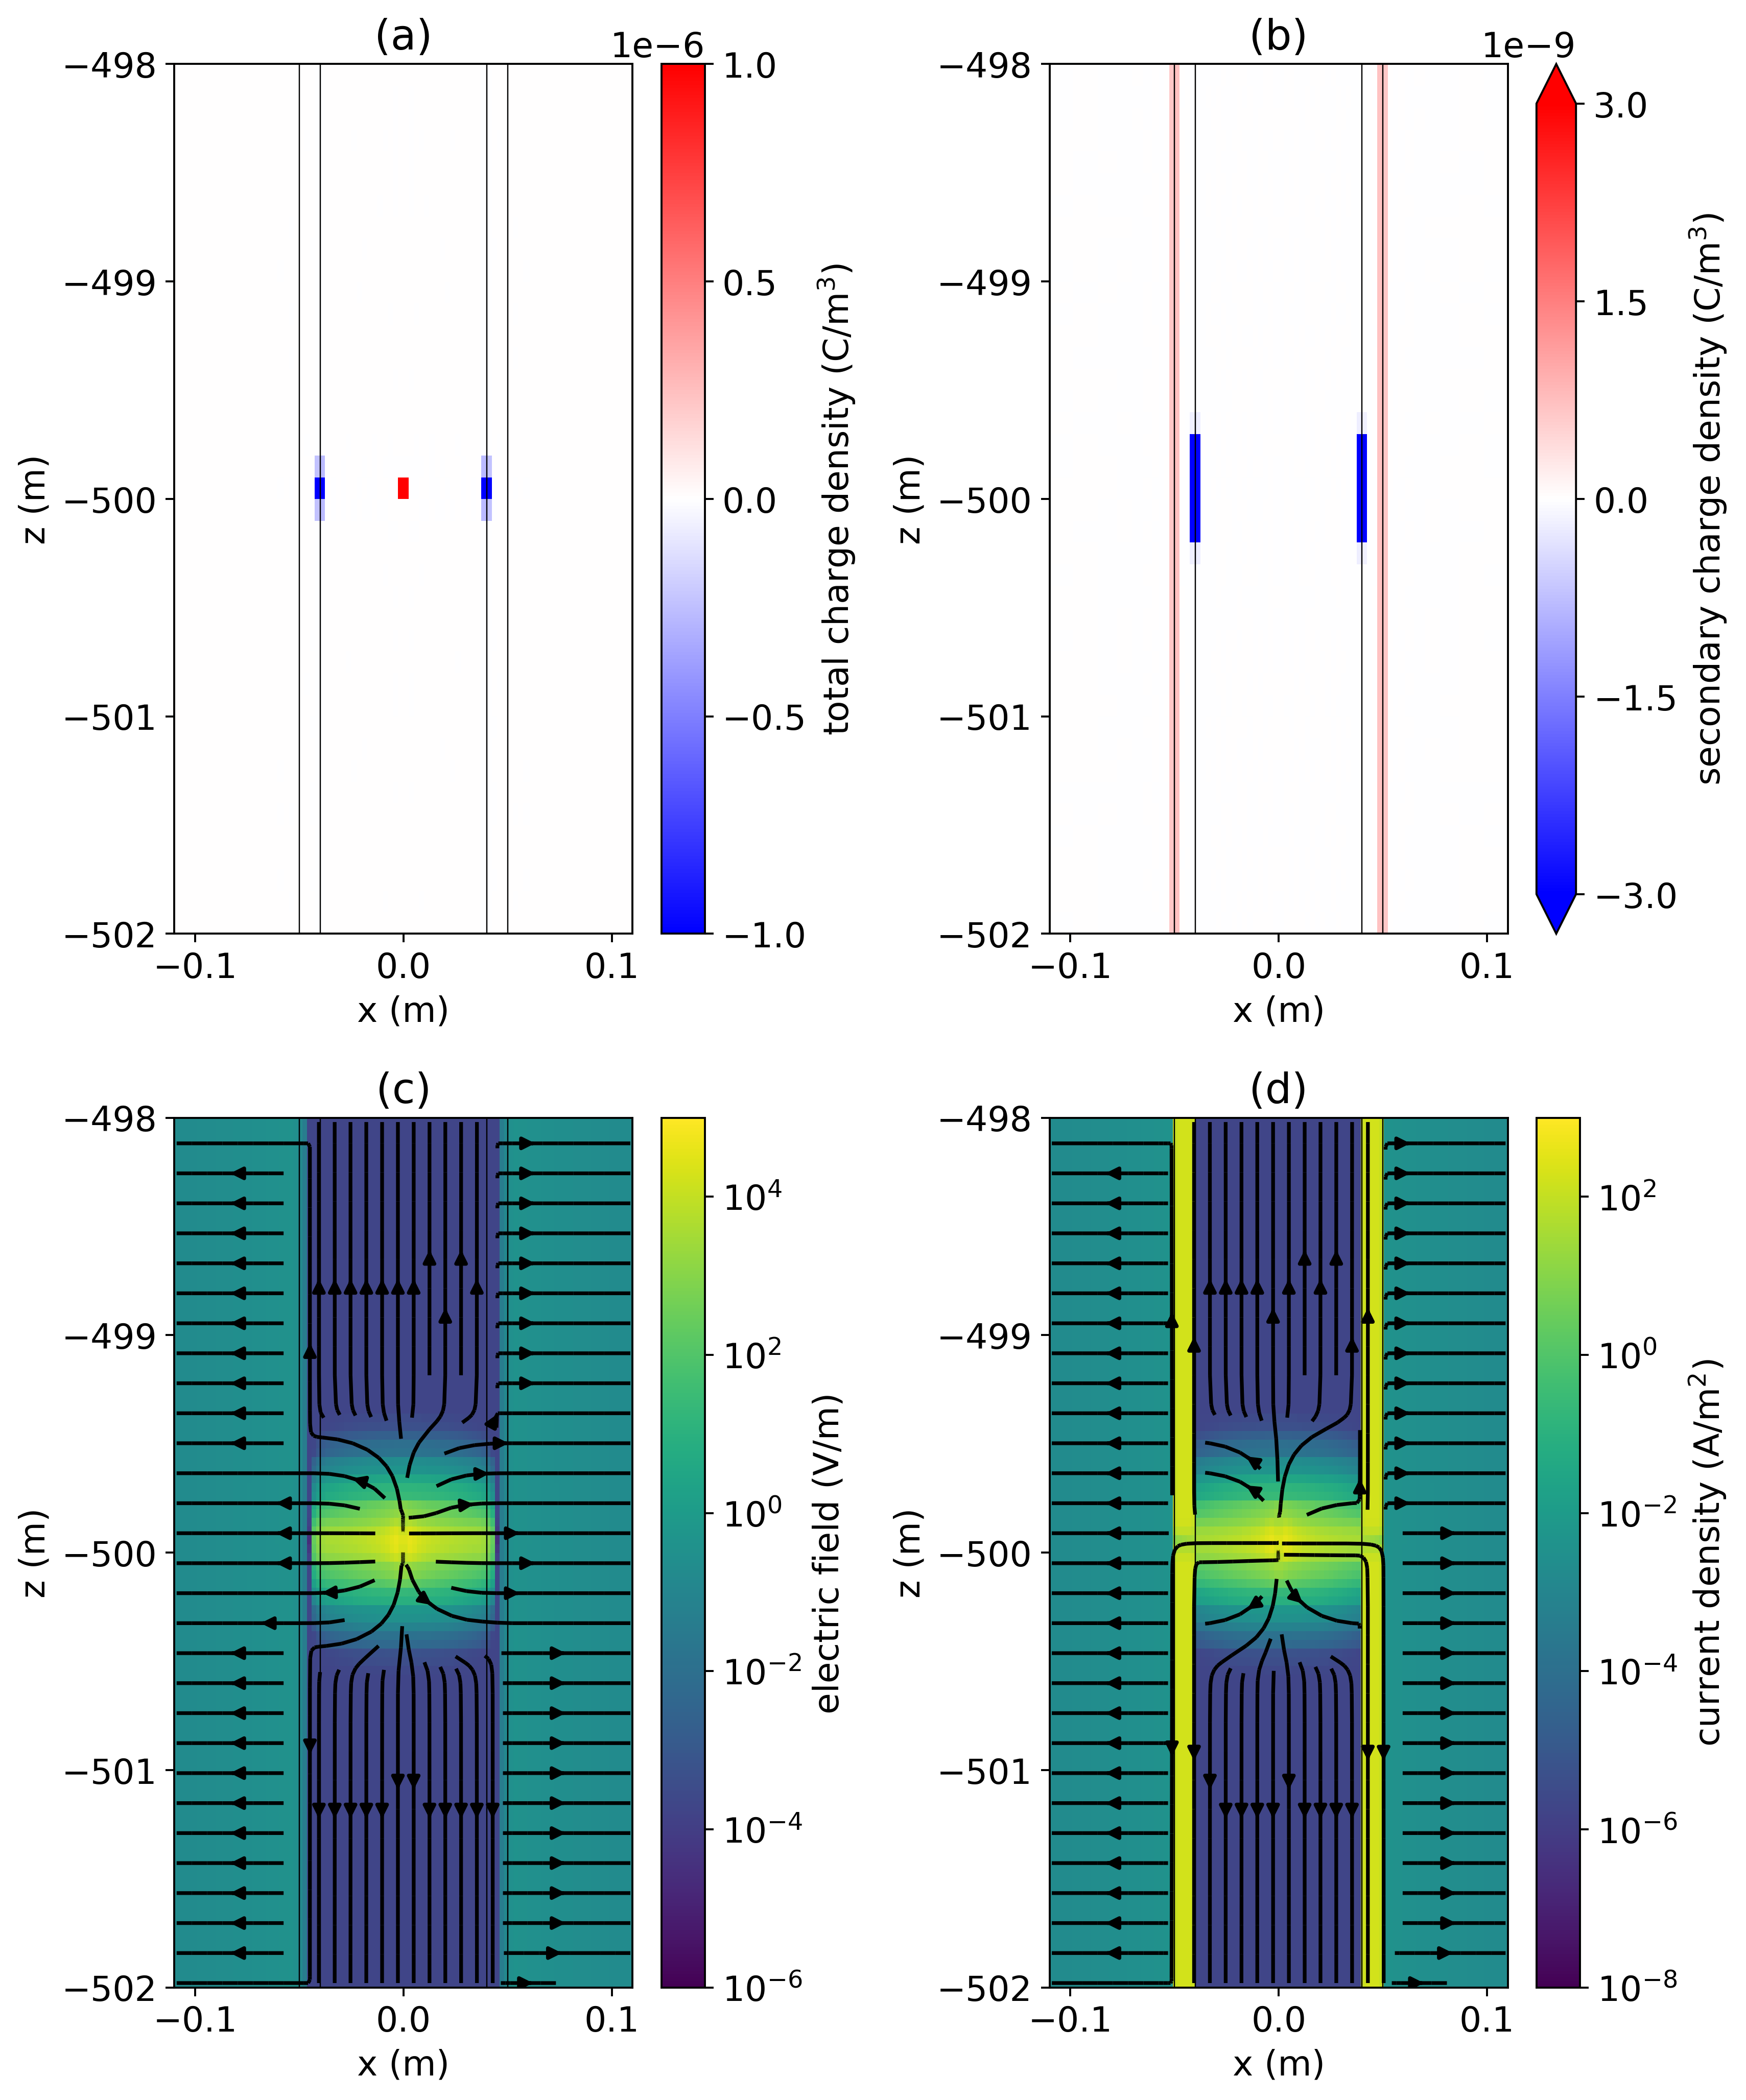
\includegraphics[width=0.7\columnwidth]{figures/casing_software/kaufman_zones.png}
    \end{center}
\caption{(a) Total charge density, (b) secondary charge density, (c) electric field, and (d) current density in a section of the pipe near the source at z=-500m.}
\label{fig:kaufman_zones}
\end{figure}

\subsubsection{Discussion}

Within the near-zone, the total charge is dominated by the large positive charge at the current electrode location and negative charges that exist along the casing wall where current is moving from a resistive region inside the borehole into a conductor. The extent of the negative charges along the inner casing wall is more evident when we look at the secondary charge, which is obtained by subtracting the charge that would be observed in a uniform half-space from the total charge (Figure \ref{fig:kaufman_zones}b). Inside the casing, we can see the transition from near-zone behavior to intermediate zone behavior approximately 0.5 m above and below the source; that is equal to 10 borehole radii from the source location, which agrees with Kaufman's conclusion.

In the intermediate zone, Kaufman discusses a number of interesting aspects with respect to  the behavior of the electric fields and currents which we can compare with the observed behavior in Figure \ref{fig:kaufman_zones}. Among them, he shows that the electric field within the borehole and casing is directed along the vertical axis; as a result no charges accumulate on the inner casing wall. Charges do, however, accumulate on the outer surface of the casing; these  generate radially-directed electric fields and currents, often referred to as “leakage currents”, within the formation. At each depth slice through the casing and borehole, the electric field is uniform, however, due to the high conductivity of the casing, most of the current flows within the casing.  The vertical extent of the intermediate zone depends on the resistivity contrast between the casing and the surrounding formation and extends beyond several hundred meters before transitioning to the far zone, where the influence of the casing disappears \citep{Kaufman1990}.

The radially directed fields from the casing, and the length of the intermediate zone, have practical implications in the context of well-logging because they delineate the region in which measurements can be made to acquire information about the formation resistivity outside the well. Within the intermediate zone, fields behave like those due to a transmission line \citep{Kaufman1990}, and multiple authors have adopted modelling strategies that approximate the well and surrounding medium as a transmission line \citep{Kong2009, Aldridge2015}. I will extend this analysis in the next example and discuss how the length of the well impacts the behavior of the charges, fields, and fluxes.
\subsection{DC Resistivity Part 2: Finite Length Wells}
\label{sec:dc_resistivity_part2}

In \citep{Kaufman1993}, the transmission-line analysis was extended to consider finite-length wells. Inspired by the interest in using the casing as an ``extended electrode'' for delivering current to depth (e.g. \cite{Schenkel1994, Um2015, Weiss2016, hoversten2017borehole}), here I consider a 3D DC resistivity experiment where one electrode is connected to the top of the well. I will examine the current and charge distribution for wells ranging in length from 250 m to 4000 m and compare those to the observations in \citep{Kaufman1993}. The conductivity of the well is selected to be $10^6$ S/m. A uniform background conductivity of $10^{-2}$ S/m is used and the return electrode is positioned 8000 m from the well; this is sufficiently far from the well that we do not need to examine the impact of the return electrode location in this example. A 3D cylindrical mesh was used for the simulation.

\cite{Kaufman1993} derives a solution for the current within a finite length well and discusses two end-member cases: a short well and a long well. ``Short'' versus ``long'' are defined on the product of $\alpha L_c$, where $L_c$ is the length of the casing and $\alpha = 1/\sqrt{S T}$, where $S$ is the cross-sectional conductance of the casing and has units of S$\cdot$m ($S = \sigma_c 2\pi a \Delta a$, for a casing with radius $a$ and thickness $\Delta a$), and $T$ is the transverse resistance. The transverse resistance is approximately equal to the resistivity of the surrounding formation (for more discussion on where this approximation breaks down, see \cite{Schenkel1994}). For short wells, $\alpha L_c \ll 1$, the current decreases linearly with distance, whereas for long wells, where $\alpha L_c \gg 1$, the current decays exponentially with distance from the source, with the rate of decay being controlled by the parameter $\alpha$. In Figure \ref{fig:kaufman_finite_well} (a), I show current in the well for 5 different borehole lengths. The x-axis is the distance from the source normalized by the length of the well. I also show the two end-member solutions (equations 45 and 53) from \cite{Kaufman1993}. There is significant overlap between the 250m numerical solution and the short well approximation. As the length of the well increases, exponential decay of the currents becomes evident. Since $\alpha$ is quite small, for this example $\alpha = 2 \times 10^{-3} ~ m^{-1}$, the borehole must be very long to reach the other end member which corresponds to the exponentially decaying solution.


\begin{figure}[htb]
    \begin{center}
    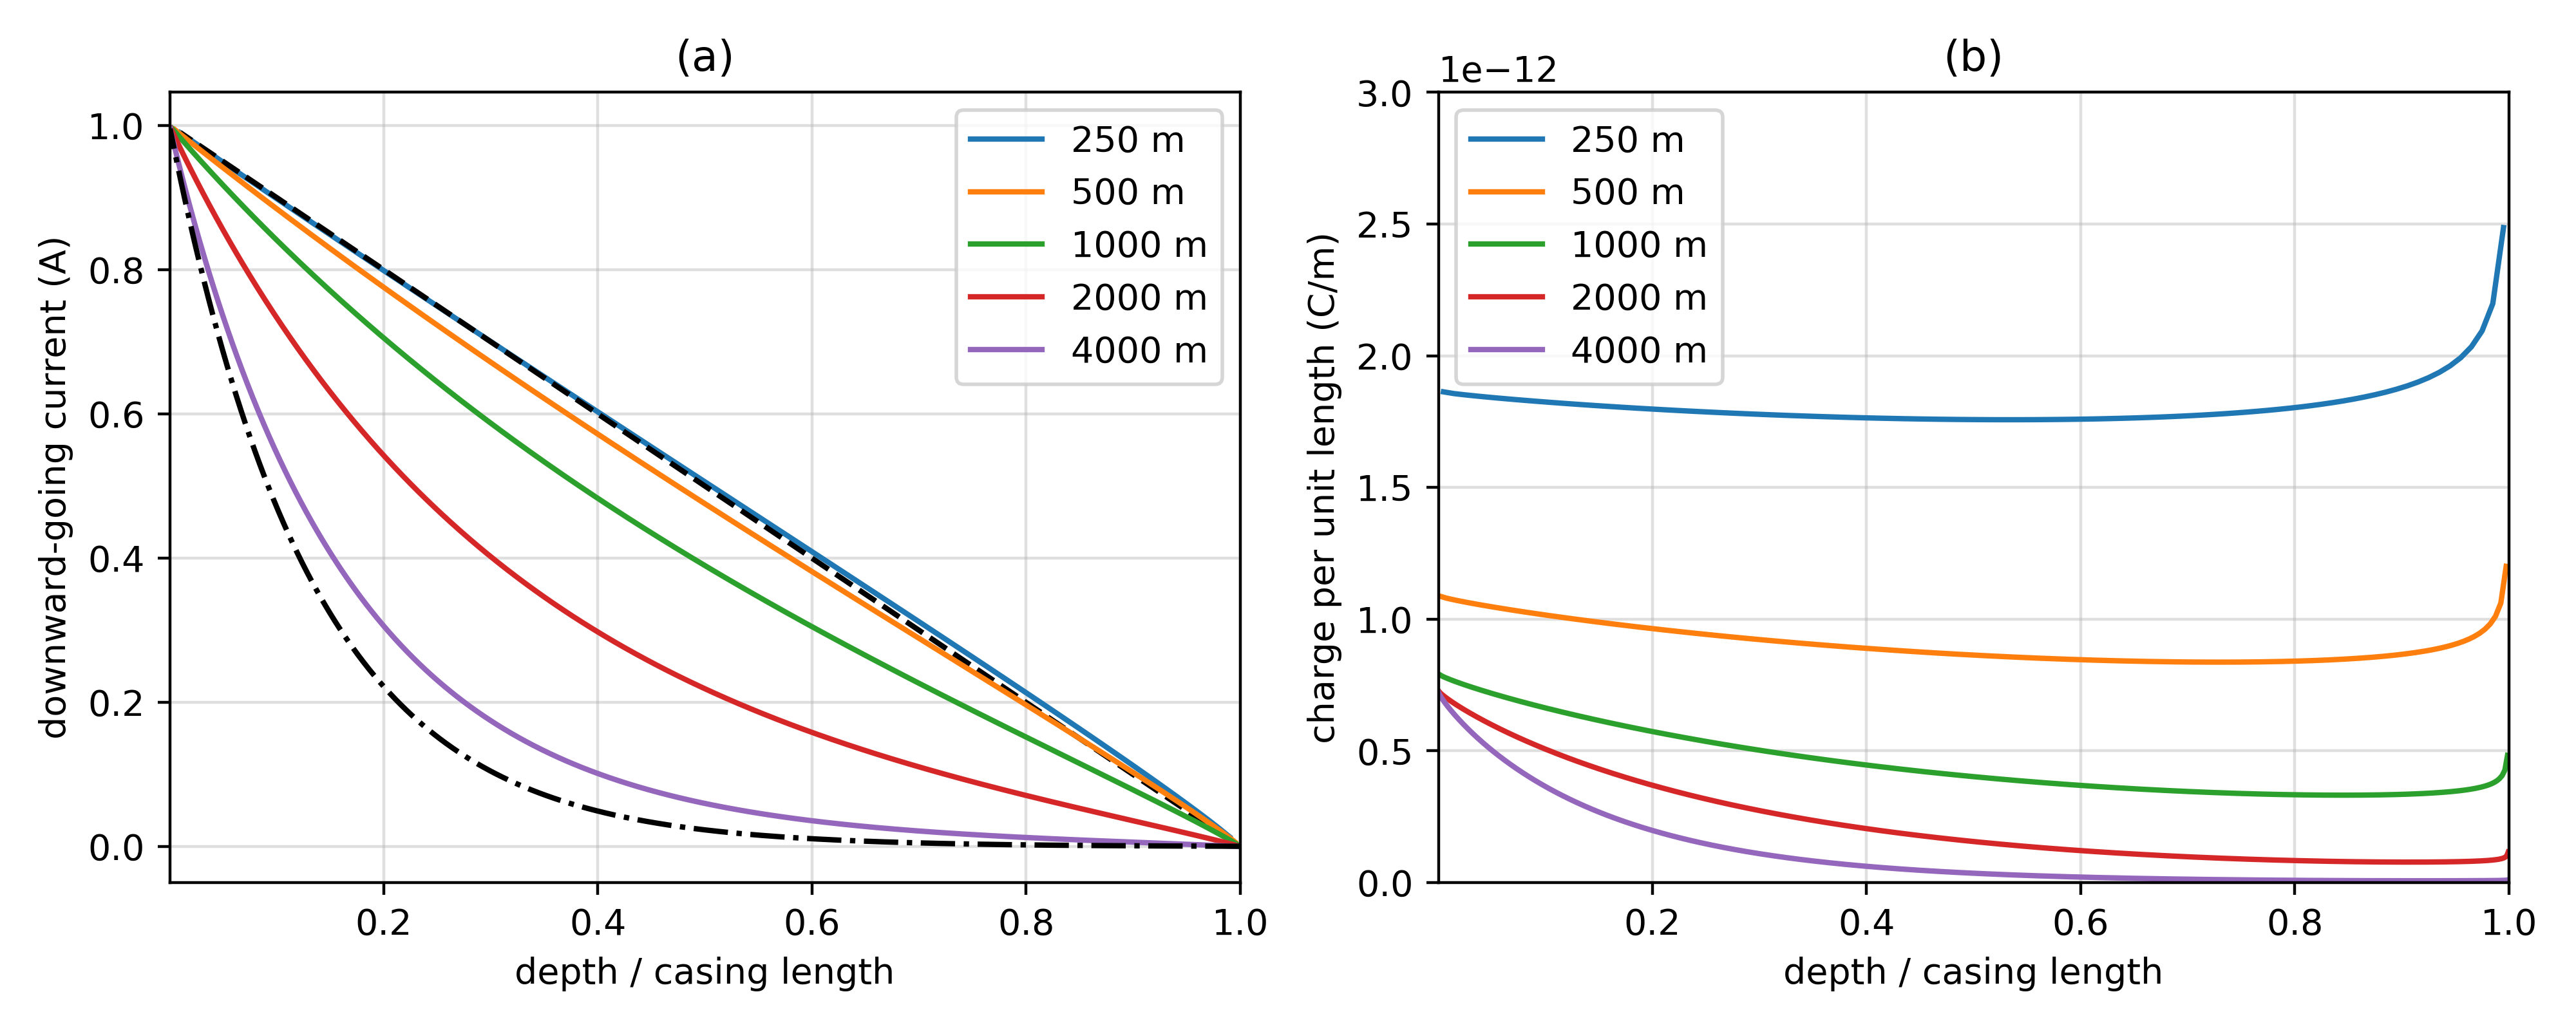
\includegraphics[width=\columnwidth]{figures/kaufman_finite_well.png}
    \end{center}
\caption{
    (a) Current along a well for 5 different wellbore lengths.
    The x-axis is depth normalized by the length of the well. The black
    dashed line shows the short-well approximation (equation 45 in \cite{Kaufman1993})
    for a 200m long well. The black dash-dot line shows the long-well approximation
    (equation 53 in \cite{Kaufman1993}) for a 4000m well.
    (b) Charge per unit length along the well for 5 different wellbore lengths.
}
\label{fig:kaufman_finite_well}
\end{figure}


In Figure \ref{fig:kaufman_finite_well} (b), I have plotted the charges along the length of the well. In the short-well regime, the borehole is approximately an equipotential surface and the charges are uniformly distributed; in the long well the charges decay with depth. What was surprising to me was the noticeable increase in charge accumulation that occurs near the bottom of the well. This is especially evident for the short well. Initially, I was suspicious and thought this might be due to problems with our numerical simulation; there was no obvious physical explanation that I was aware of. However, investigation into the literature revealed that the increase in charge density at the ends of a cylinder is a real physical effect, but an exact theoretical solution does still not appear to exist \citep{Griffiths1997} (see figure 4, in particular).

\subsubsection{Discussion}

The results shown in Figure \ref{fig:kaufman_finite_well} have implications when testing approaches for reducing computational load by approximating a well with a solid tube or prism, as in \cite{Um2015}, or replacing the well with a distribution of charges, as in \cite{Weiss2016}. For a short well, the behaviour of the currents is independent of conductivity, so, as long as the borehole is approximated by a sufficiently conductive target, the behaviour of the fields and fluxes will be representative of the fine-scale model. However, as the length of the well increases, the cross-sectional conductance of the well becomes relevant as it controls the rate of decay of the currents in the well and thus the rate that currents leak into the formation. A similar result holds when a line of charges is used to approximate the well as a DC source; a uniform charge is suitable for a sufficiently short or sufficiently conductive well, whereas a distribution of charge which decays exponentially with depth needs to be considered for longer wells. Thus, when attempting to replace a fine-scale model of a well with a coarse-scale model, either with a conductivity structure or by some form of ``equivalent source'', validations should be performed on models that have the same length-scale as the experiment to ensure that both behaviors are being accurately modeled.

\subsection{Frequency Domain Electromagnetics Part 1: Comparison with scale model results}
\label{sec:FDEM_part1}

In the DC example, we discussed how charges are distributed along the well and currents flow into the formation. From a historical perspective, practical developments in EM were pursued in the frequency domain; the mathematics is more manageable in the frequency domain, and technological advances were being made in the development of induction well-logging tools \citep{Doll1949, Moran1962}. Although the conductivity of the pipes generally plays the most dominant role in attenuating the signal, the magnetic permeability is non-negligible \citep{Wait1977}; it is the product of the conductivity and permeability that appears in the description of EM attenuation. Also, the fact that permeable material becomes magnetized in the presence of an external field complicates the problem.
\cite{Augustin1989} is one of the first papers on induction logging in the presence of steel cased wells that aims to understand and isolate the EM response of the steel cased well. Using a combination of scale modelling and analytical mathematical modelling, they examine the impacts of conductivity and magnetic permeability on the magnetic field observed in the pipe. In this example and the one that follows, I attempt to unravel this interplay between conductivity and magnetic permeability.

The first experiment \cite{Augustin1989} discusses is a scale model using two different pipes, a conductive copper pipe and a conductive, permeable iron pipe; each pipe is 9 m in length. The copper pipe had an inner diameter of 0.063 m and a thickness of 0.002 m, while the iron pipe had a 0.063 m inner diameter and 0.0043 m wall thickness. A source-loop, with radius 0.6 m was co-axial with the pipe and in one experiment positioned at one end of the pipe (which they refer to as the ``semi-infinite pipe'' scenario). In another experiment the source loop is positioned at the midpoint of the pipe (which they refer to as the ``infinite pipe'' scenario); for both experiments, magnetic field data are measured as a function of frequency at the central axis of the pipe. Their results are presented in terms of a Field Strength Ratio (FSR), which is the ratio of the absolute value of the magnetic field at the receiver with the absolute value of the magnetic field if no pipe is present (Figure 3 in \cite{Augustin1989}). At low frequencies, for the data collected within the iron pipe, static shielding (FSR $<$ 1) was observed for the measurements where the receiver was in the plane of the source loop for both the ``infinite'' and ``semi-infinite'' scenarios. When the receiver was positioned within the pipe, 1.49 m offset from the plane of the source loop, static enhancement effects (FSR $>$ 1) were observed for both the infinite and semi-infinite scenarios. Using this experiment for context, I will compare the behaviour of our numerical simulation with the observations in \citep{Augustin1989} and examine the nature of the static shielding and enhancement effects.

For our numerical setup, the pipes are 9 m in length and have an inner diameter of 0.06 m. The copper pipe has a casing-wall thickness of 0.002 m and the iron pipe has a thickness of 0.004 m. Following the estimated physical property values from \cite{Augustin1989}, I use a conductivity of $3.5 \times 10^7$ S/m and a relative permeability of 1 for the copper pipe. For the iron pipe, a conductivity of $8.0 \times 10^6$ S/m and a relative permeability of 150 is used. A background resistivity of $10^4 ~\Omega$m is assumed. The computed FSR values for the axial magnetic field as a function of frequency are shown in Figure \ref{fig:AugustinFSR}.


\begin{figure}
    \begin{center}
    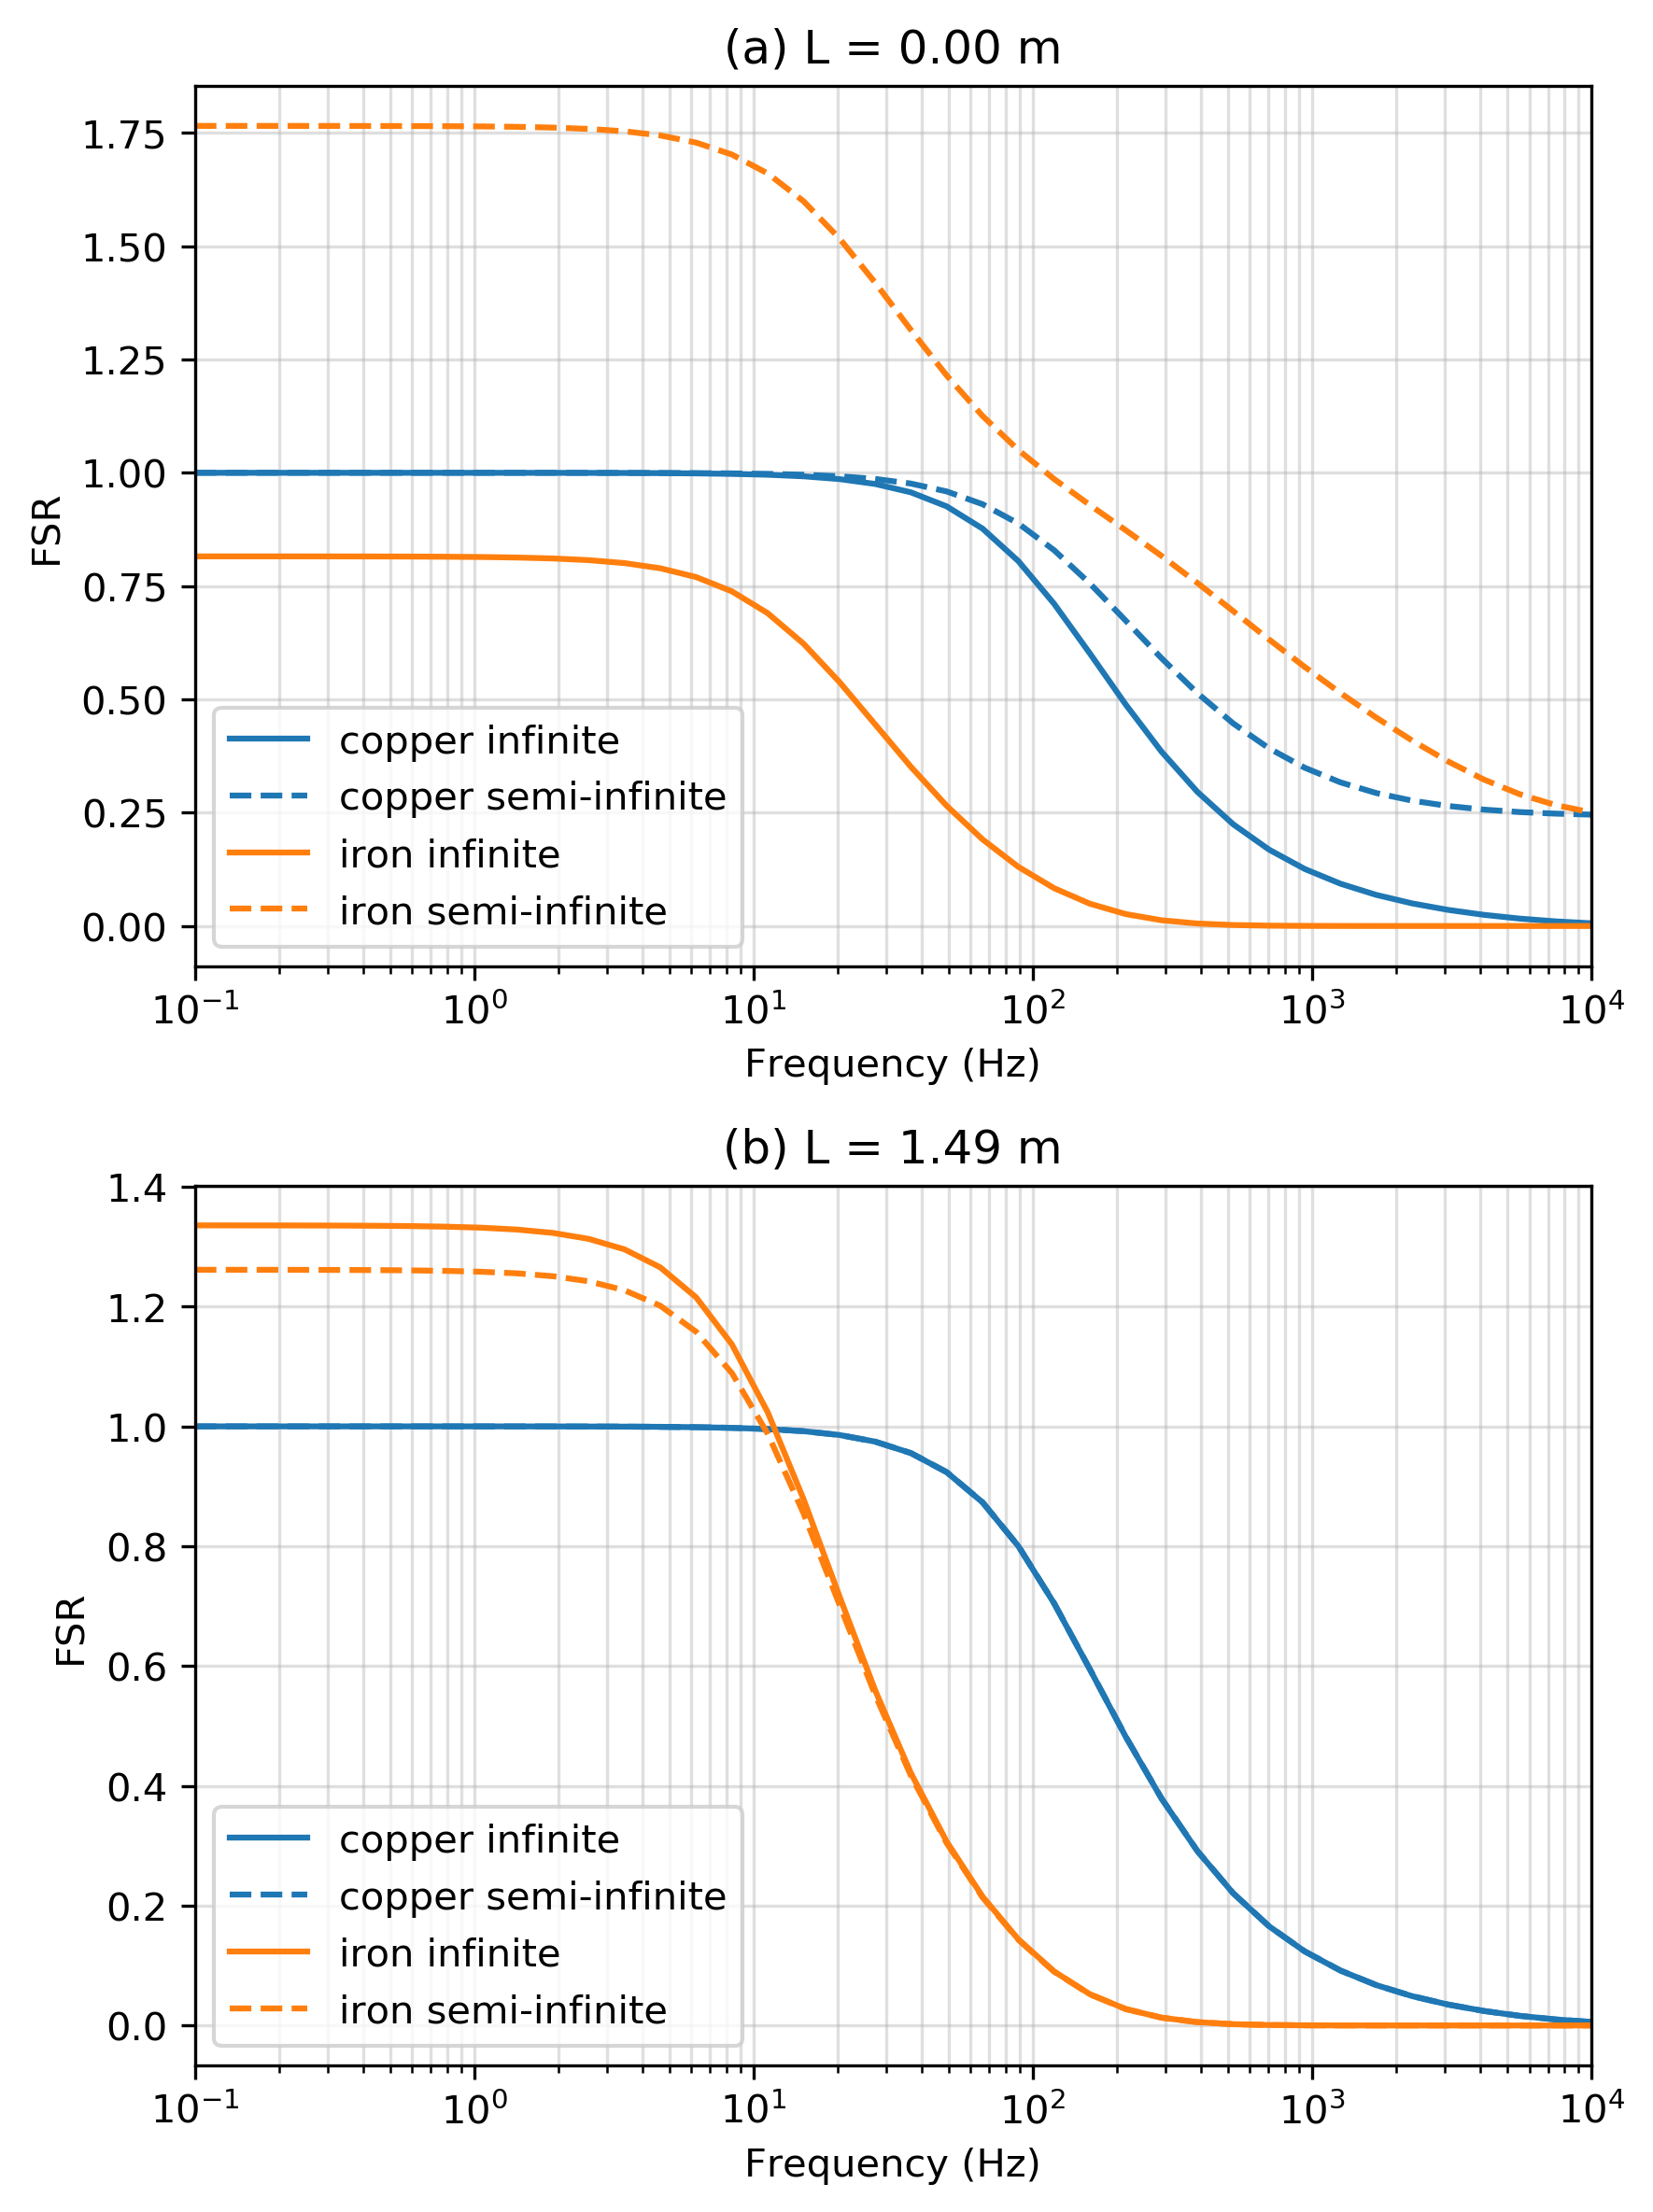
\includegraphics[width=0.6\columnwidth]{figures/casing_software/AugustinFSR.png}
    \end{center}
\caption{
    Field strength ratio (FSR), the ratio of the measured vertical magnetic field with the free space magnetic field, as a function of frequency for two different reciever locations.
    In (a), the reciever is in the same plane as the source, in (b), the reciever is 1.49m offset from the source.
}
\label{fig:AugustinFSR}
\end{figure}


Consider the response of the conductive pipe. At low frequencies, the FSR for the copper pipe (blue lines) is 1 for both the infinite (solid line) and semi-infinite (dashed line) scenarios, as the field inside the copper pipe is equivalent to the free-space field. With increasing frequency, eddy currents are induced in the pipe which generate a magnetic field that opposes the primary, causing a decrease in the observed FSR. When the source and receiver are in the same plane (L=0.00 m), the rate of decrease is more rapid in the infinite scenario than the semi-infinite. Since there is conductive material on both sides of the receiver in the infinite case, we would expect attenuation of the fields to occur more rapidly than in the semi-infinite case. This observation is consistent with Figure 3a in \cite{Augustin1989}. For the offset receiver (L=1.49 m), they observed a slight separation in the infinite and semi-infinite curves which I do not; however, they attributed this to potential errors in magnetometer position. Thus, overall, the numerical results for the copper pipe are in good agreement with the scale model results observed by \cite{Augustin1989}.

Next, we examine the response of the conductive, permeable pipe. In Figure \ref{fig:AugustinFSR}b, we observe a static enhancement effect (FSR $>$ 1) at low frequencies. The enhancement is larger in the infinite scenario than the semi-infinite scenario; this is in agreement with Figure 3b in \cite{Augustin1989}. There is however, a significant discrepancy between our numerical simulations and the scale model for the semi-infinite pipe when the source and receiver lie in the same plane(Figure \ref{fig:AugustinFSR}a). \cite{Augustin1989} observed a static shielding effect for both the infinite and semi-infinite scenarios, whereas we observe a static shielding for the infinite scenario, but a significant static enhancement for the semi-infinite case. To examine what might be the cause of this, I will examine the magnetic flux density in this region of the pipe.

In Figure \ref{fig:AugustinBfields}, I have plotted: (a) the secondary magnetic flux in the infinite-pipe scenario near the source ($z=$-4.5 m), (b) the secondary magnetic flux in the semi-infinite scenario (z=0 m for the source), and (c) top 5 cm of the semi-infinite pipe. All plots are at 0.1 Hz. The primary magnetic field is directed upwards within the regions I have plotted, so upward-going magnetic flux indicates a static enhancement effect, and downward-oriented magnetic flux indicates static shielding effects. In (a) we see a transition between the static shielding in the vicinity of the source to a static enhancement approximately 0.5 m above and below the plane of the source. Similarly in (b), we notice a sign-reversal in the z-component of the secondary magnetic flux at a depth of 0.6 m.

\subsubsection{Discussion}
The behaviors observed in Figure \ref{fig:AugustinBfields} are quite comparable to Augustin et al.'s observation of a transition from shielding to enhancement occurring at distances greater than 0.8 m from the source. Numerical experiments show that the vertical extent of the region over which static shielding is occurring increases with increasing pipe diameter, and similarly increases with increasing loop radius while the magnitude of the effect decreases. This can be understood by considering how the pipe is magnetized; for a small loop radius, the magnetization is largely localized near the plane of the source and rapidly falls off with distance from the plane of the source. Localized, large amplitude magnetization causes the casing to act as a collection of dipoles around the circumference of the casing. As the radius of the loop increases, the magnetization spreads out along the length of the well resulting in longer, lower-amplitude dipoles, thus both increasing the extent of the region over which static shielding is occurring as well as decreasing its amplitude.


\begin{figure}
    \begin{center}
    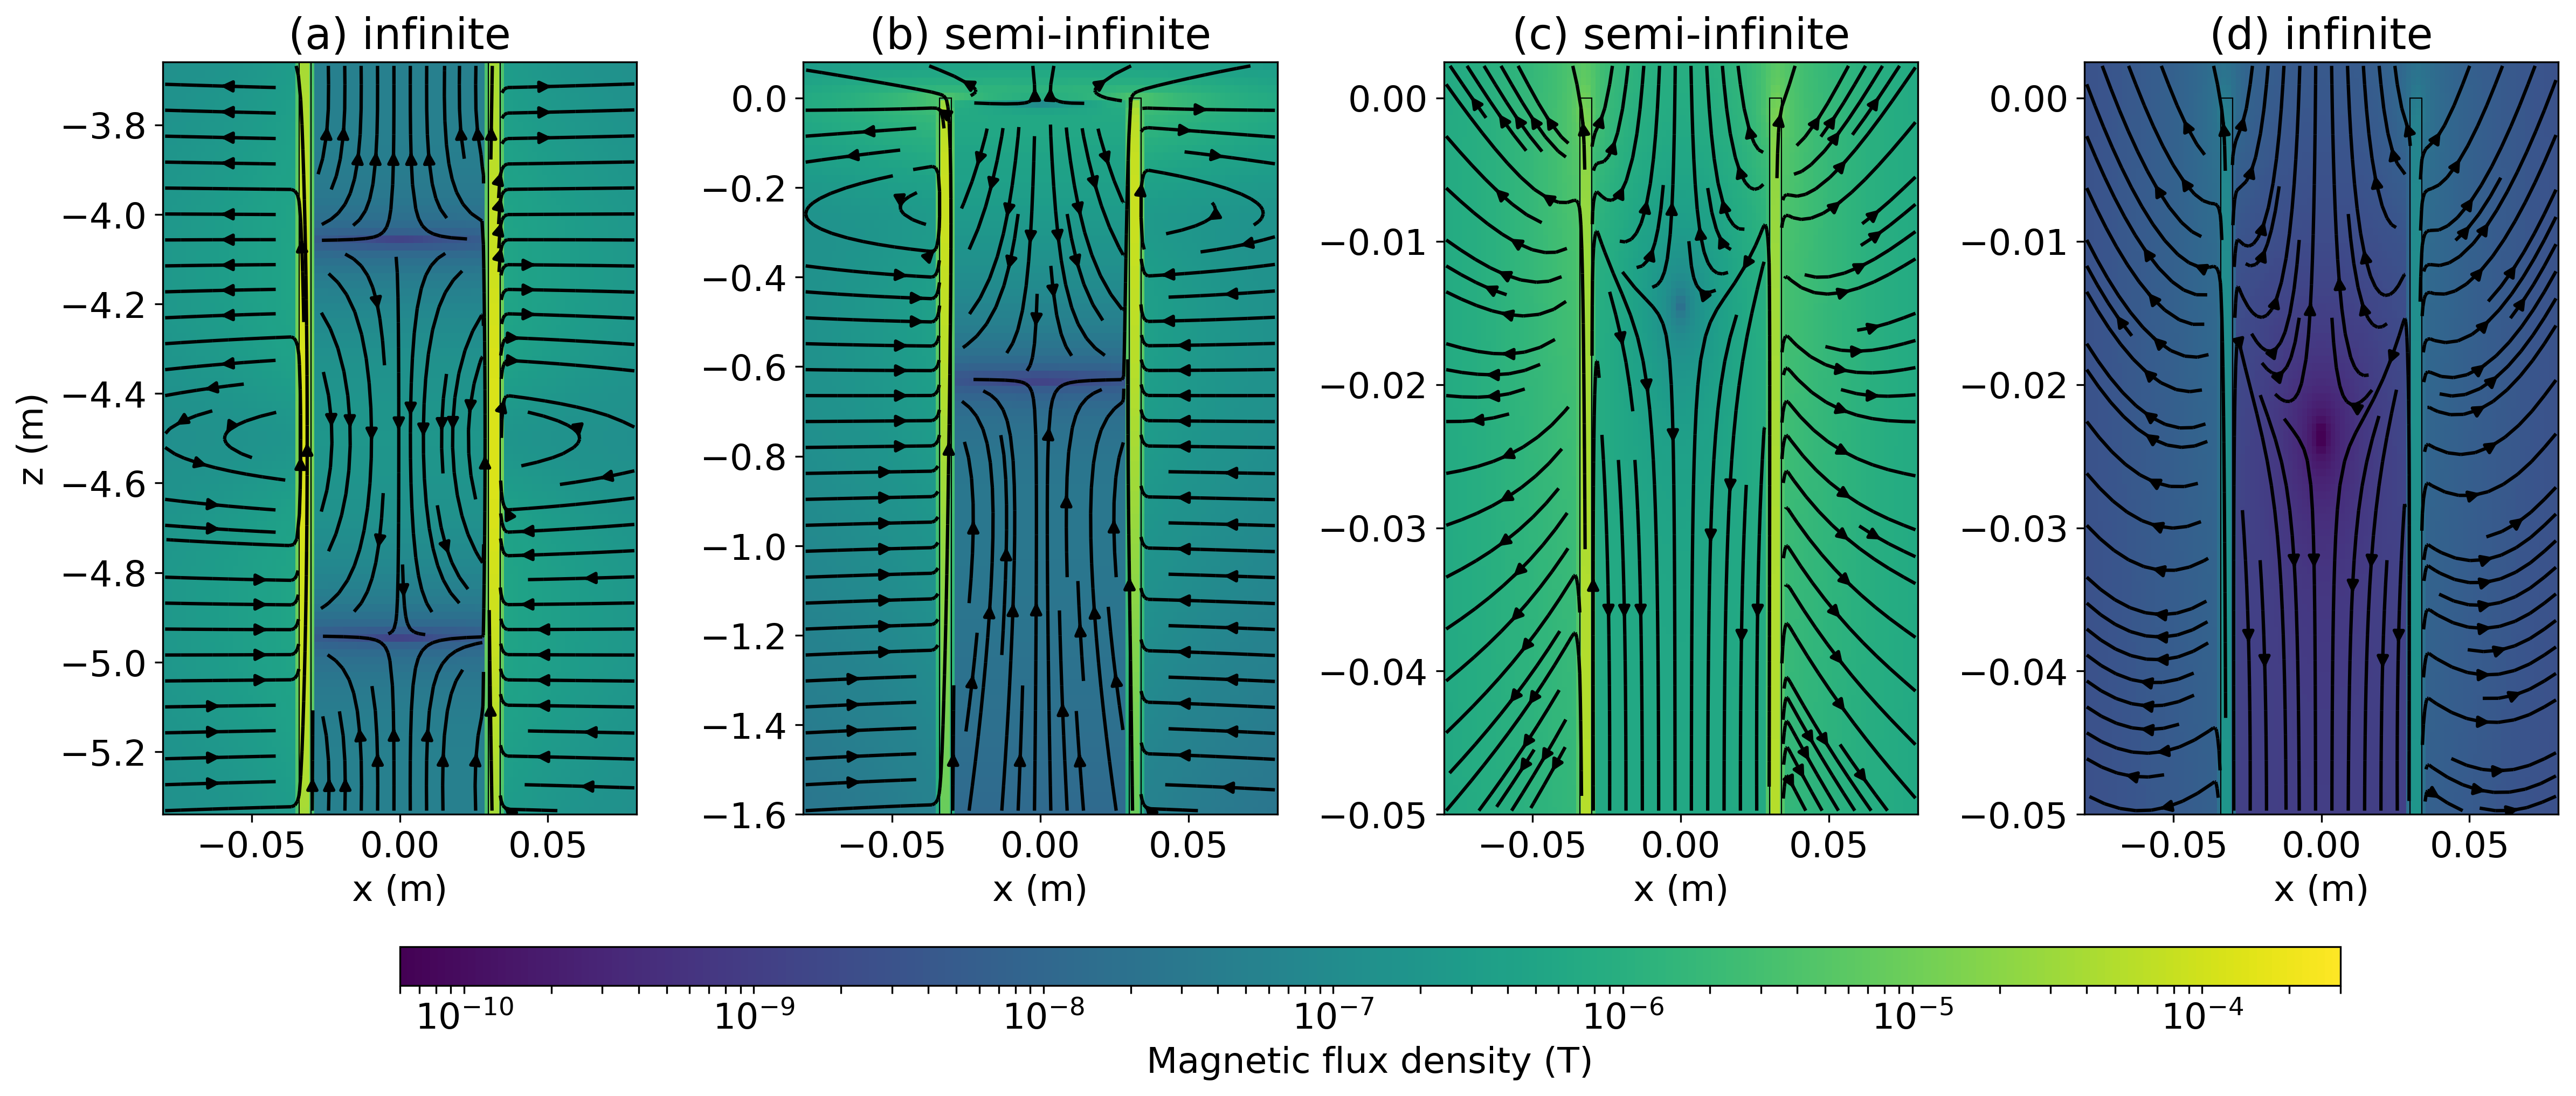
\includegraphics[width=\columnwidth]{figures/casing_software/AugustinBfields.png}
    \end{center}
\caption{
    Magnetic flux density at 0.1 Hz in the region of the pipe near the plane of the source for
    (a) the ``infinite'' pipe, where the source is located at -4.5 m and the pipe extends from 0 m to -9 m,
    (b) a ``semi-infinite'' pipe, where the source is located at 0 m and the pipe extends to -9 m.
    In (c), we zoom in to the top 5 cm of the ``semi-infinite'' pipe,
    and (d) shows the 5 cm at the top-end of the ``infinite'' pipe.
}
\label{fig:AugustinBfields}
\end{figure}


This explains the nature of the static enhancement and static shielding effects, but to explain the discrepancy between the static shielding observed in the semi-infinite pipe when L=0 m by Augustin et al., and the static enhancement we observe in Figure \ref{fig:AugustinFSR}a, I examine the magnetic flux density in the top few centimeters of the pipe. Figure \ref{fig:AugustinBfields}c shows the top 5 cm of the secondary magnetic flux in the semi-infinite pipe; the source is in the z=0 m plane.  Zooming in reveals there is yet another sign reversal near the end of the pipe. This is evident even in the infinite-pipe scenario (Figure \ref{fig:AugustinFSR}d), where the source is offset by several meters from the end of the pipe. This edge-effect perhaps bears some similarities to what we observed in Figure \ref{fig:kaufman_finite_well}b, where we saw a build up of charge near the end of the pipe in the DC scenario. At the end of the pipe, we encounter the situation where the normal component of the flux ($\vec{j}, \vec{b}$) from the pipe to the background needs to be continuous both in the radial and vertical directions at the end of the pipe as does the tangential component of the fields ($\vec{e}, \vec{h}$). The interplay of these two constraints at the end of the pipe results in more complexity in the resultant fields and fluxes. Within the span of a few centimeters we transition from static enhancement at the top of the pipe to a static shielding further down. An error as small as a few centimeters in the position of the magnetometer causes a reversal in behavior; in Figure \ref{fig:Augustin3cm}, I have plotted the FSR for a magnetometer positioned 3 cm beneath the plane of the source, and the static-shielding behavior observed for the semi-infinite pipe is much more aligned with that observed in Figure 3a in \cite{Augustin1989}.



\begin{figure}
    \begin{center}
    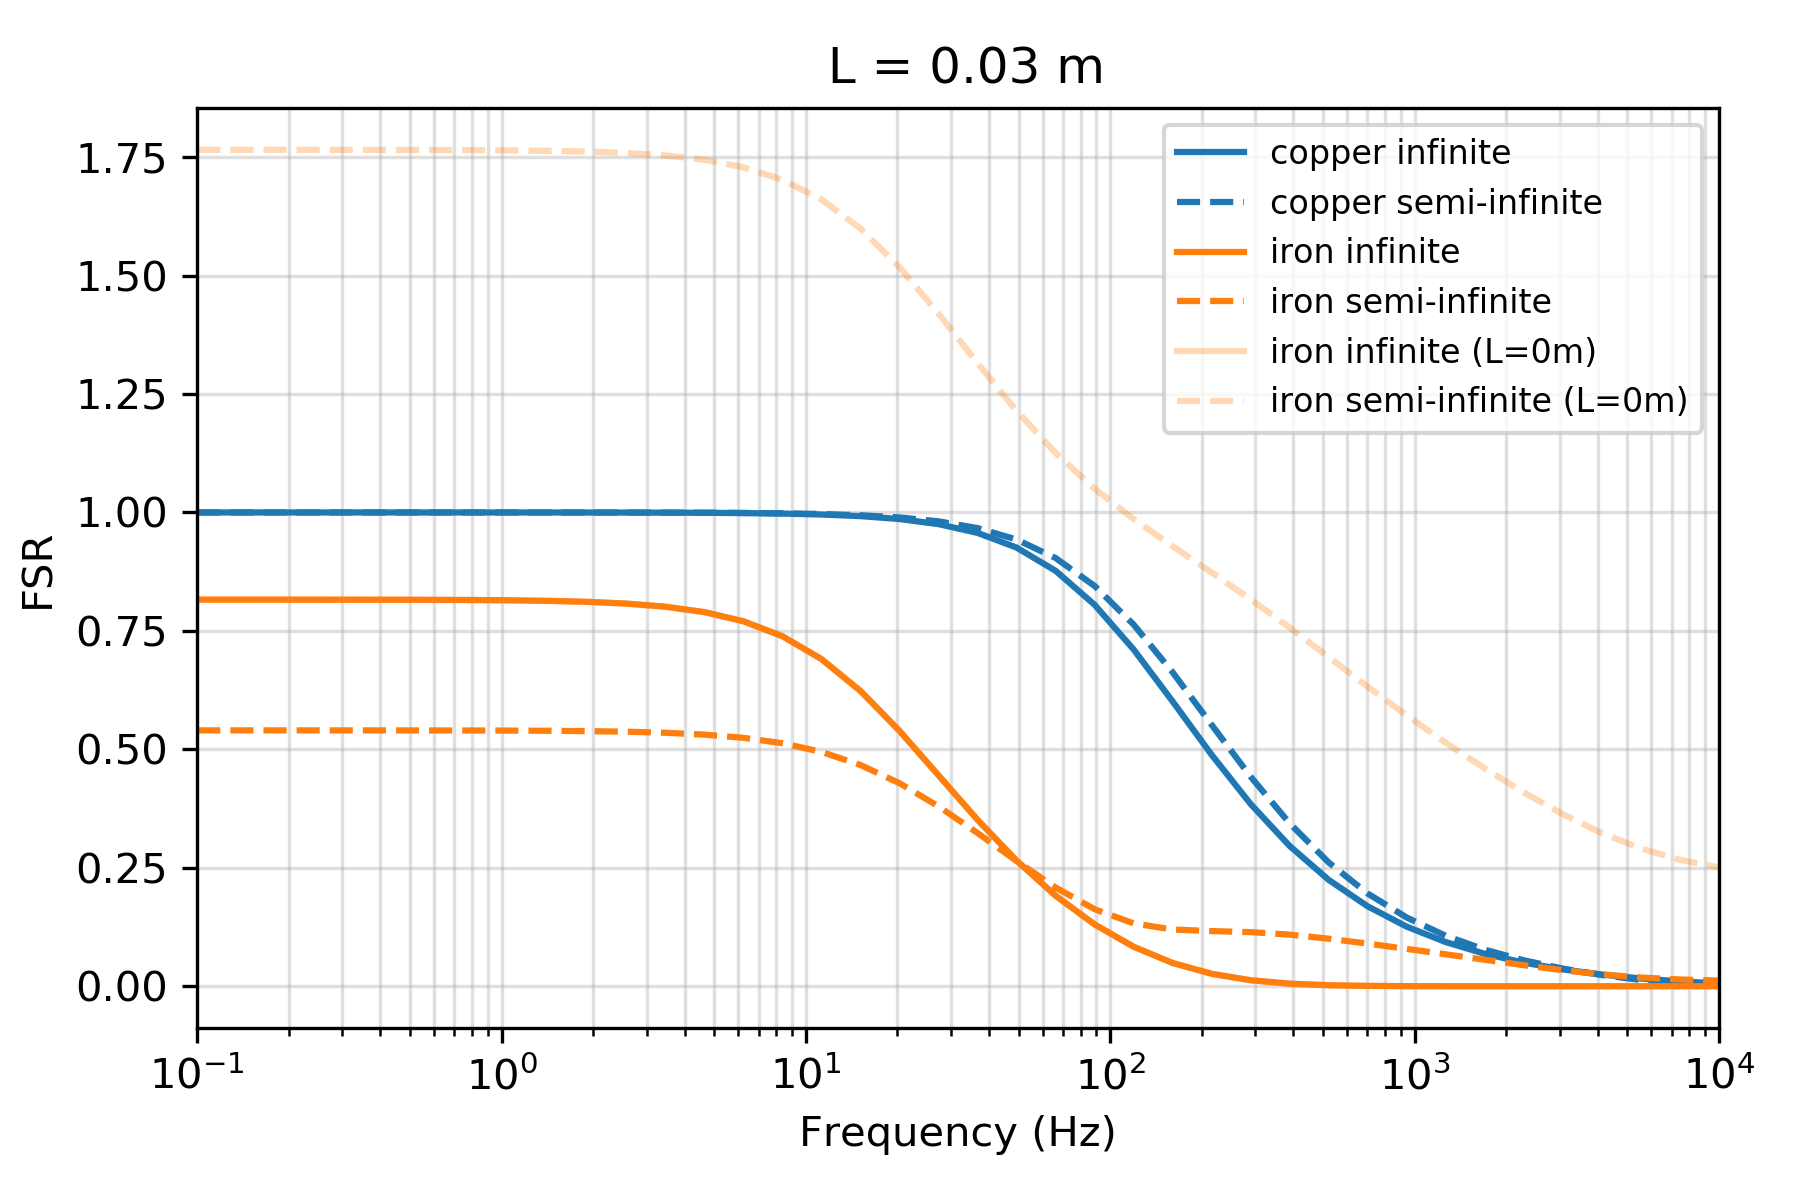
\includegraphics[width=0.6\columnwidth]{figures/Augustin3cm.png}
    \end{center}
\caption{
    Field strength ratio, FSR, for a reciever positioned 3cm beneath
    the plane of the source. For comparison, we have plotted the
    FSR for the permeable pipe when the source and reciever lie in the same
    plane (L=0.00m) with the semi-transparent orange lines.
    Note that the infinite-pipe solutions for L=0.03m and L=0.00m overlap.
}
\label{fig:Augustin3cm}
\end{figure}





\subsection{Frequency Domain Electromagnetics Part 2: Conductivity and permeability in the inductive response of a well}
\label{sec:FDEM_part2}

The experiments shown in the previous section revealed some insights into the complexity of the fields within the pipe and illustrated the role of permeability in the character of the responses at low frequency. Next, we move to larger scales and examine the role of conductivity and permeability in the responses we observe in the borehole.

In this example, I consider a 2 km long well with an outer diameter of 10 cm and thickness of 1 cm in a whole-space which has a resistivity of $10^4$ $\Omega$m. A loop with radius 100 m is coaxial with the well and positioned at the top-end of the well. A receiver measuring the z-component of the magnetic flux density is positioned 500 m below the transmitter loop, along the axis of the well. I will consider both time domain and frequency domain responses.

In electromagnetics, it is often the product of permeability and conductivity that is considered to be the main controlling factor on the EM responses. To assess the contribution of each to the measured responses, I will investigate two scenarios. In the first, the well has a conductivity of $10^8$ S/m and a relative permeability of 1, and in the second, the well has a conductivity of $10^6$ S/m and a relative permeability of 100; thus the product of conductivity and permeability is equivalent for both wells.

Similar to the analysis done by \cite{Augustin1989} when looking at the role of borehole radius in the behaviour of the magnetic response (e.g. figure 8), I will examine the normalized secondary field (NSF) which is the ratio of the secondary field with the amplitude of the primary, where the primary is defined to be the free-space response. In Figure \ref{fig:fdemNSF}, I have plotted the normalized secondary field for the two pipes considered, the conductive pipe (blue) and the conductive, permeable pipe (orange). Let us start by examining the conductivity response in Figure \ref{fig:fdemNSF}. Where the value of the NSF is zero, the primary dominates the response; this is the case at low frequencies where induction is not yet contributing to the response. As frequency increases, currents are induced in the pipe which generate a secondary magnetic field that opposes the primary, hence the NSF becomes negative. When the real part of the NSF (solid line) is -1, the secondary magnetic field is equal in magnitude but opposite in direction to the free-space primary and the measured real field is zero. Values less than -1 indicate a sign reversal in the real magnetic field. Similarly, when the imaginary part of the response function goes above zero, there is a sign reversal in the imaginary component. Note that these sign reversals occur even in a half-space and are a result of sampling the fields within a conductive medium; in this case the receiver was 500 m below the surface.

As compared to the conductive pipe, the frequency at which induction sets in is higher for the conductive, permeable pipe. We also notice that the amplitude variation of both the imaginary and real parts is larger for the permeable pipe. To examine the contribution of conductivity and permeability to the responses, I have plotted the real part of the secondary magnetic flux density, $\mathbf{b}$, in Figure \ref{fig:bfdem}. The top row shows the response within the conductive pipe and the bottom row shows the conductive, permeable pipe. The primary magnetic flux is oriented upwards and we can see that all of the secondary fields generated are oriented downwards. Similar to the previous example, we see that at low frequencies, there is magnetostatic response due to the permeable pipe. However, due to the larger length scales of the source loop and the casing in this example, there is no measurable contribution at the receiver. At 1 Hz, we can see that induction is starting to contribute to the signal for the conductive pipe, while for the permeable pipe, it is not until $\sim$10 Hz that we begin to observe the contribution of induction. At 100 Hz, the secondary magnetic field is stronger in amplitude than the primary, and the NFS is less than -1 for both the conductive and permeable pipes. The amplitude of the secondary within the permeable pipe is stronger than that in the conductive pipe. At 1000 Hz, we have reached the asymptote of NSF=-1 for both the conductive and permeable pipes; the secondary magnetic flux is equal in magnitude but opposite in direction to the primary.

\begin{figure}[htb]
    \begin{center}
    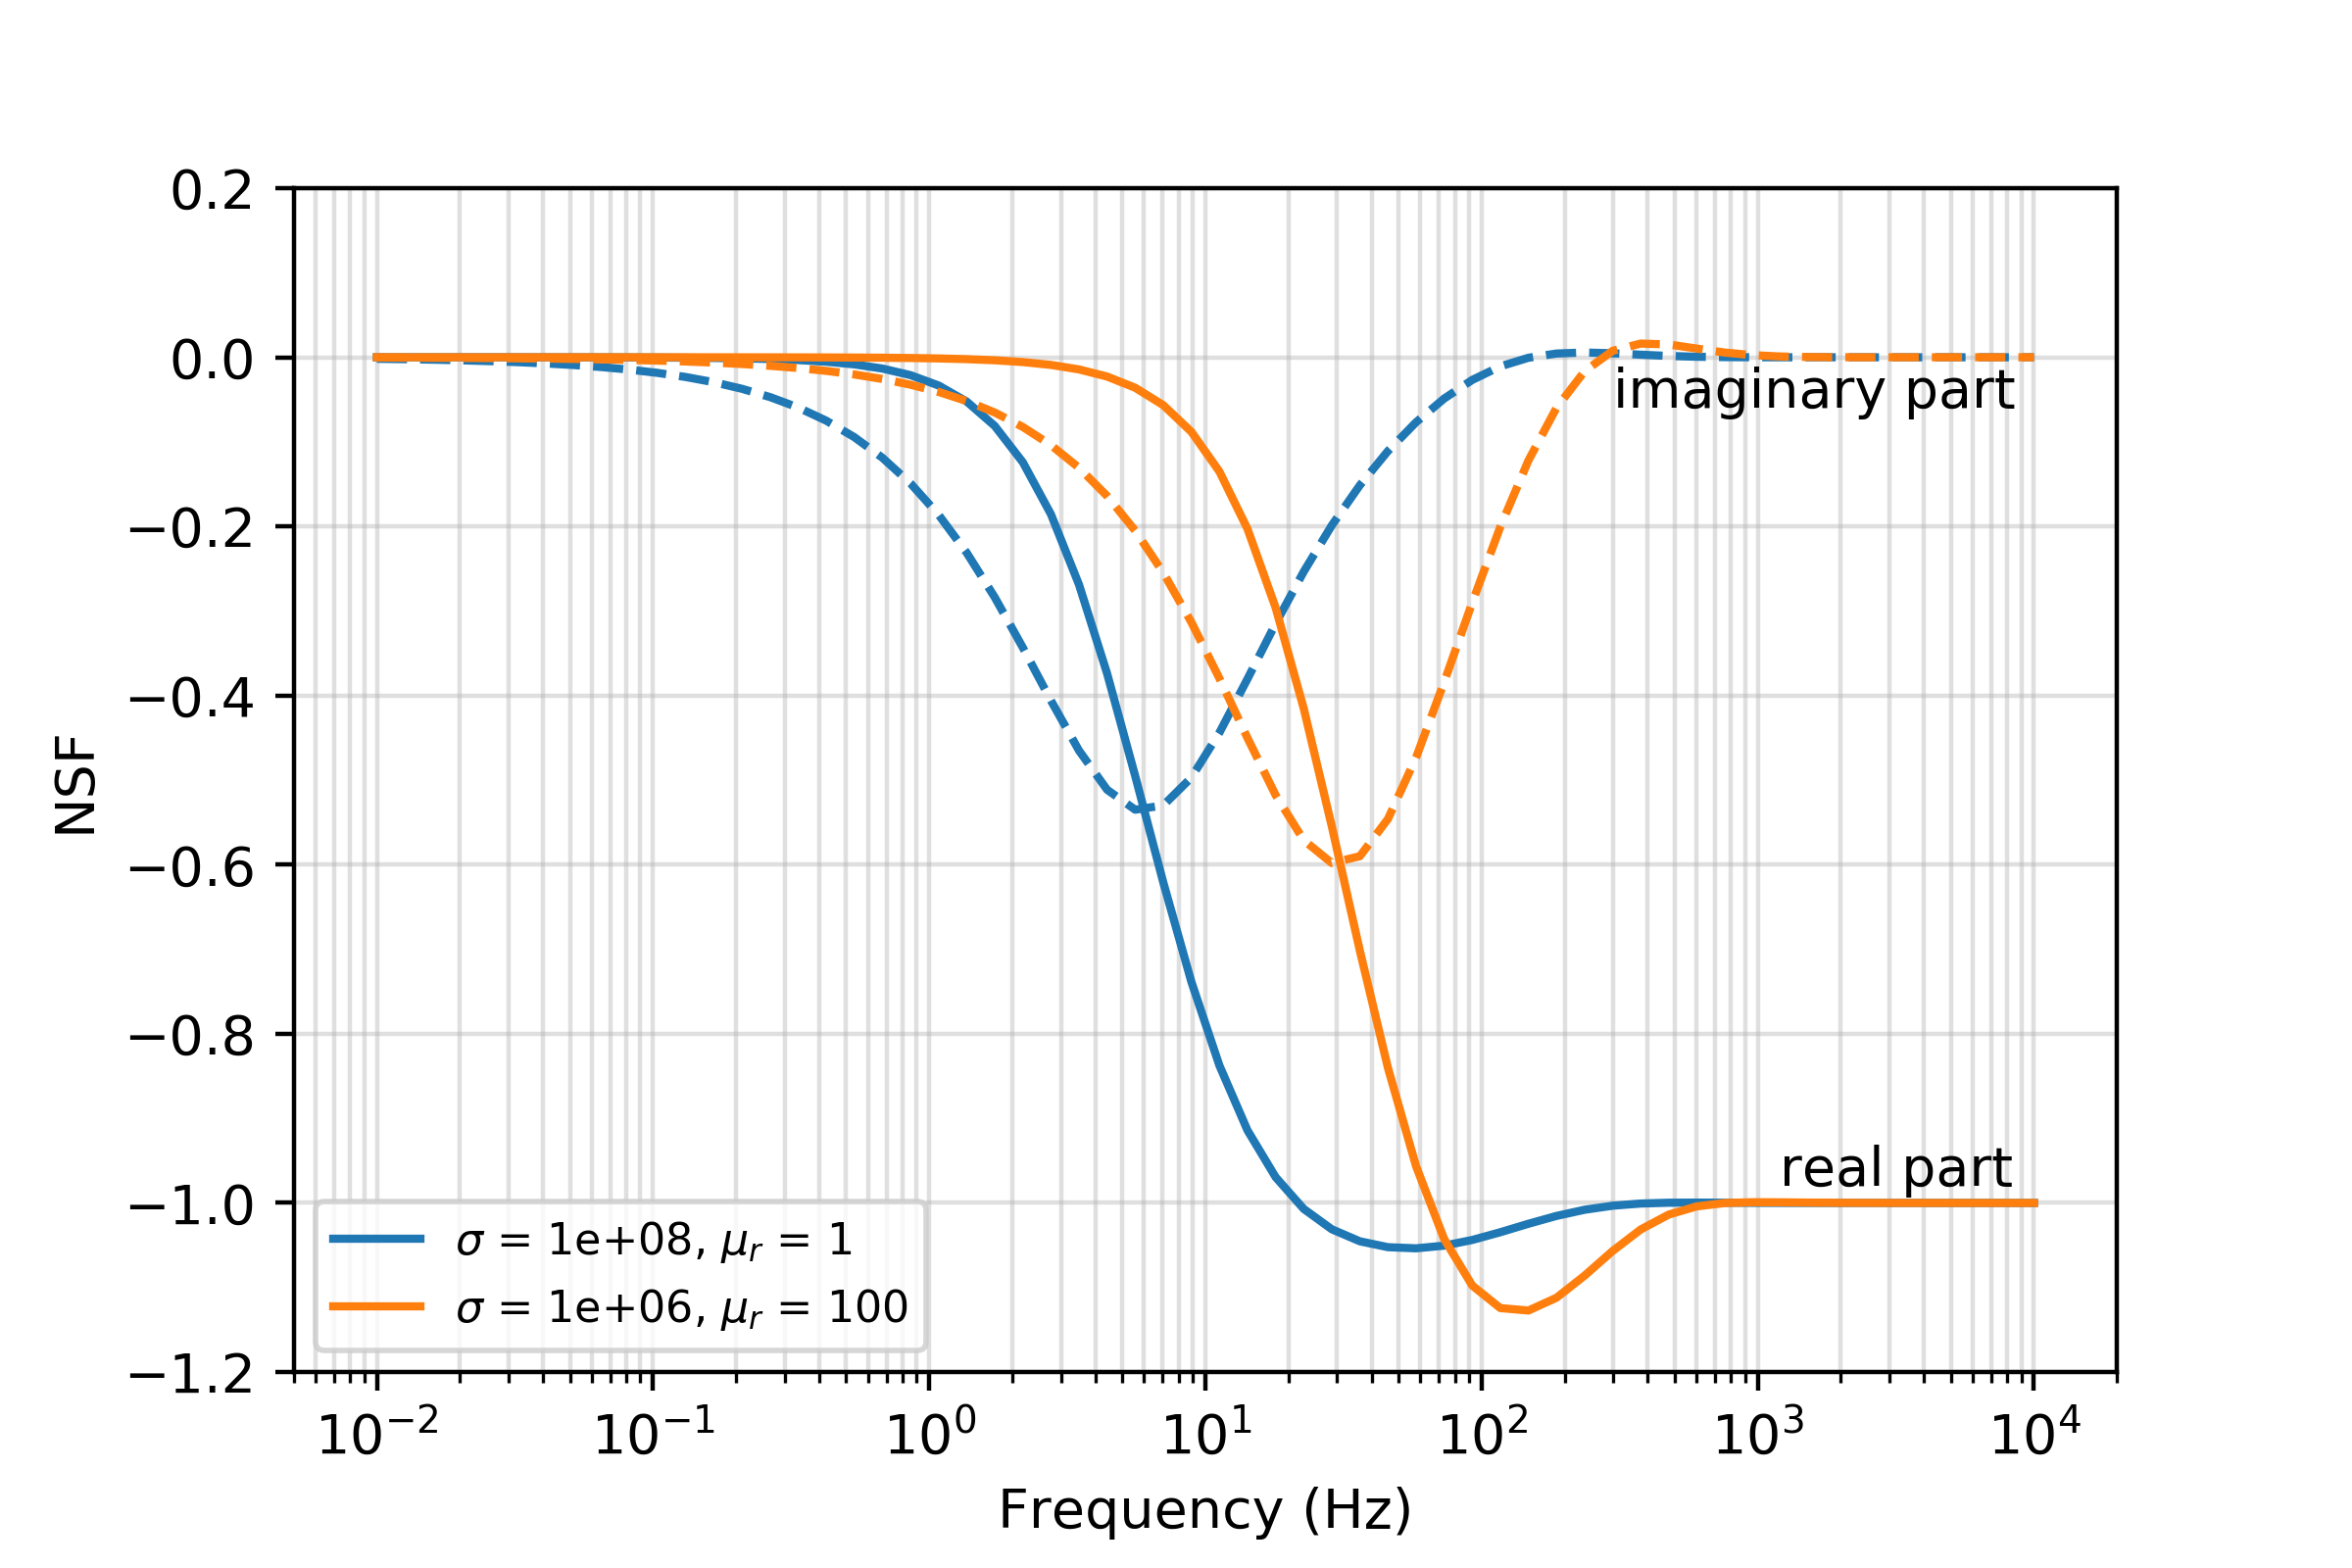
\includegraphics[width=0.6\columnwidth]{figures/casing_software/fdemNSF.png}
    \end{center}
\caption{
    Normalized secondary field, NSF, as a function of frequency for two wells.
    The NSF is the ratio of the secondary vertical magnetic field with the primary magnetic field at the receiver location ($z=$-500 m);
    the primary is defined as the whole-space primary.
}
\label{fig:fdemNSF}
\end{figure}



\begin{figure}
    \begin{center}
    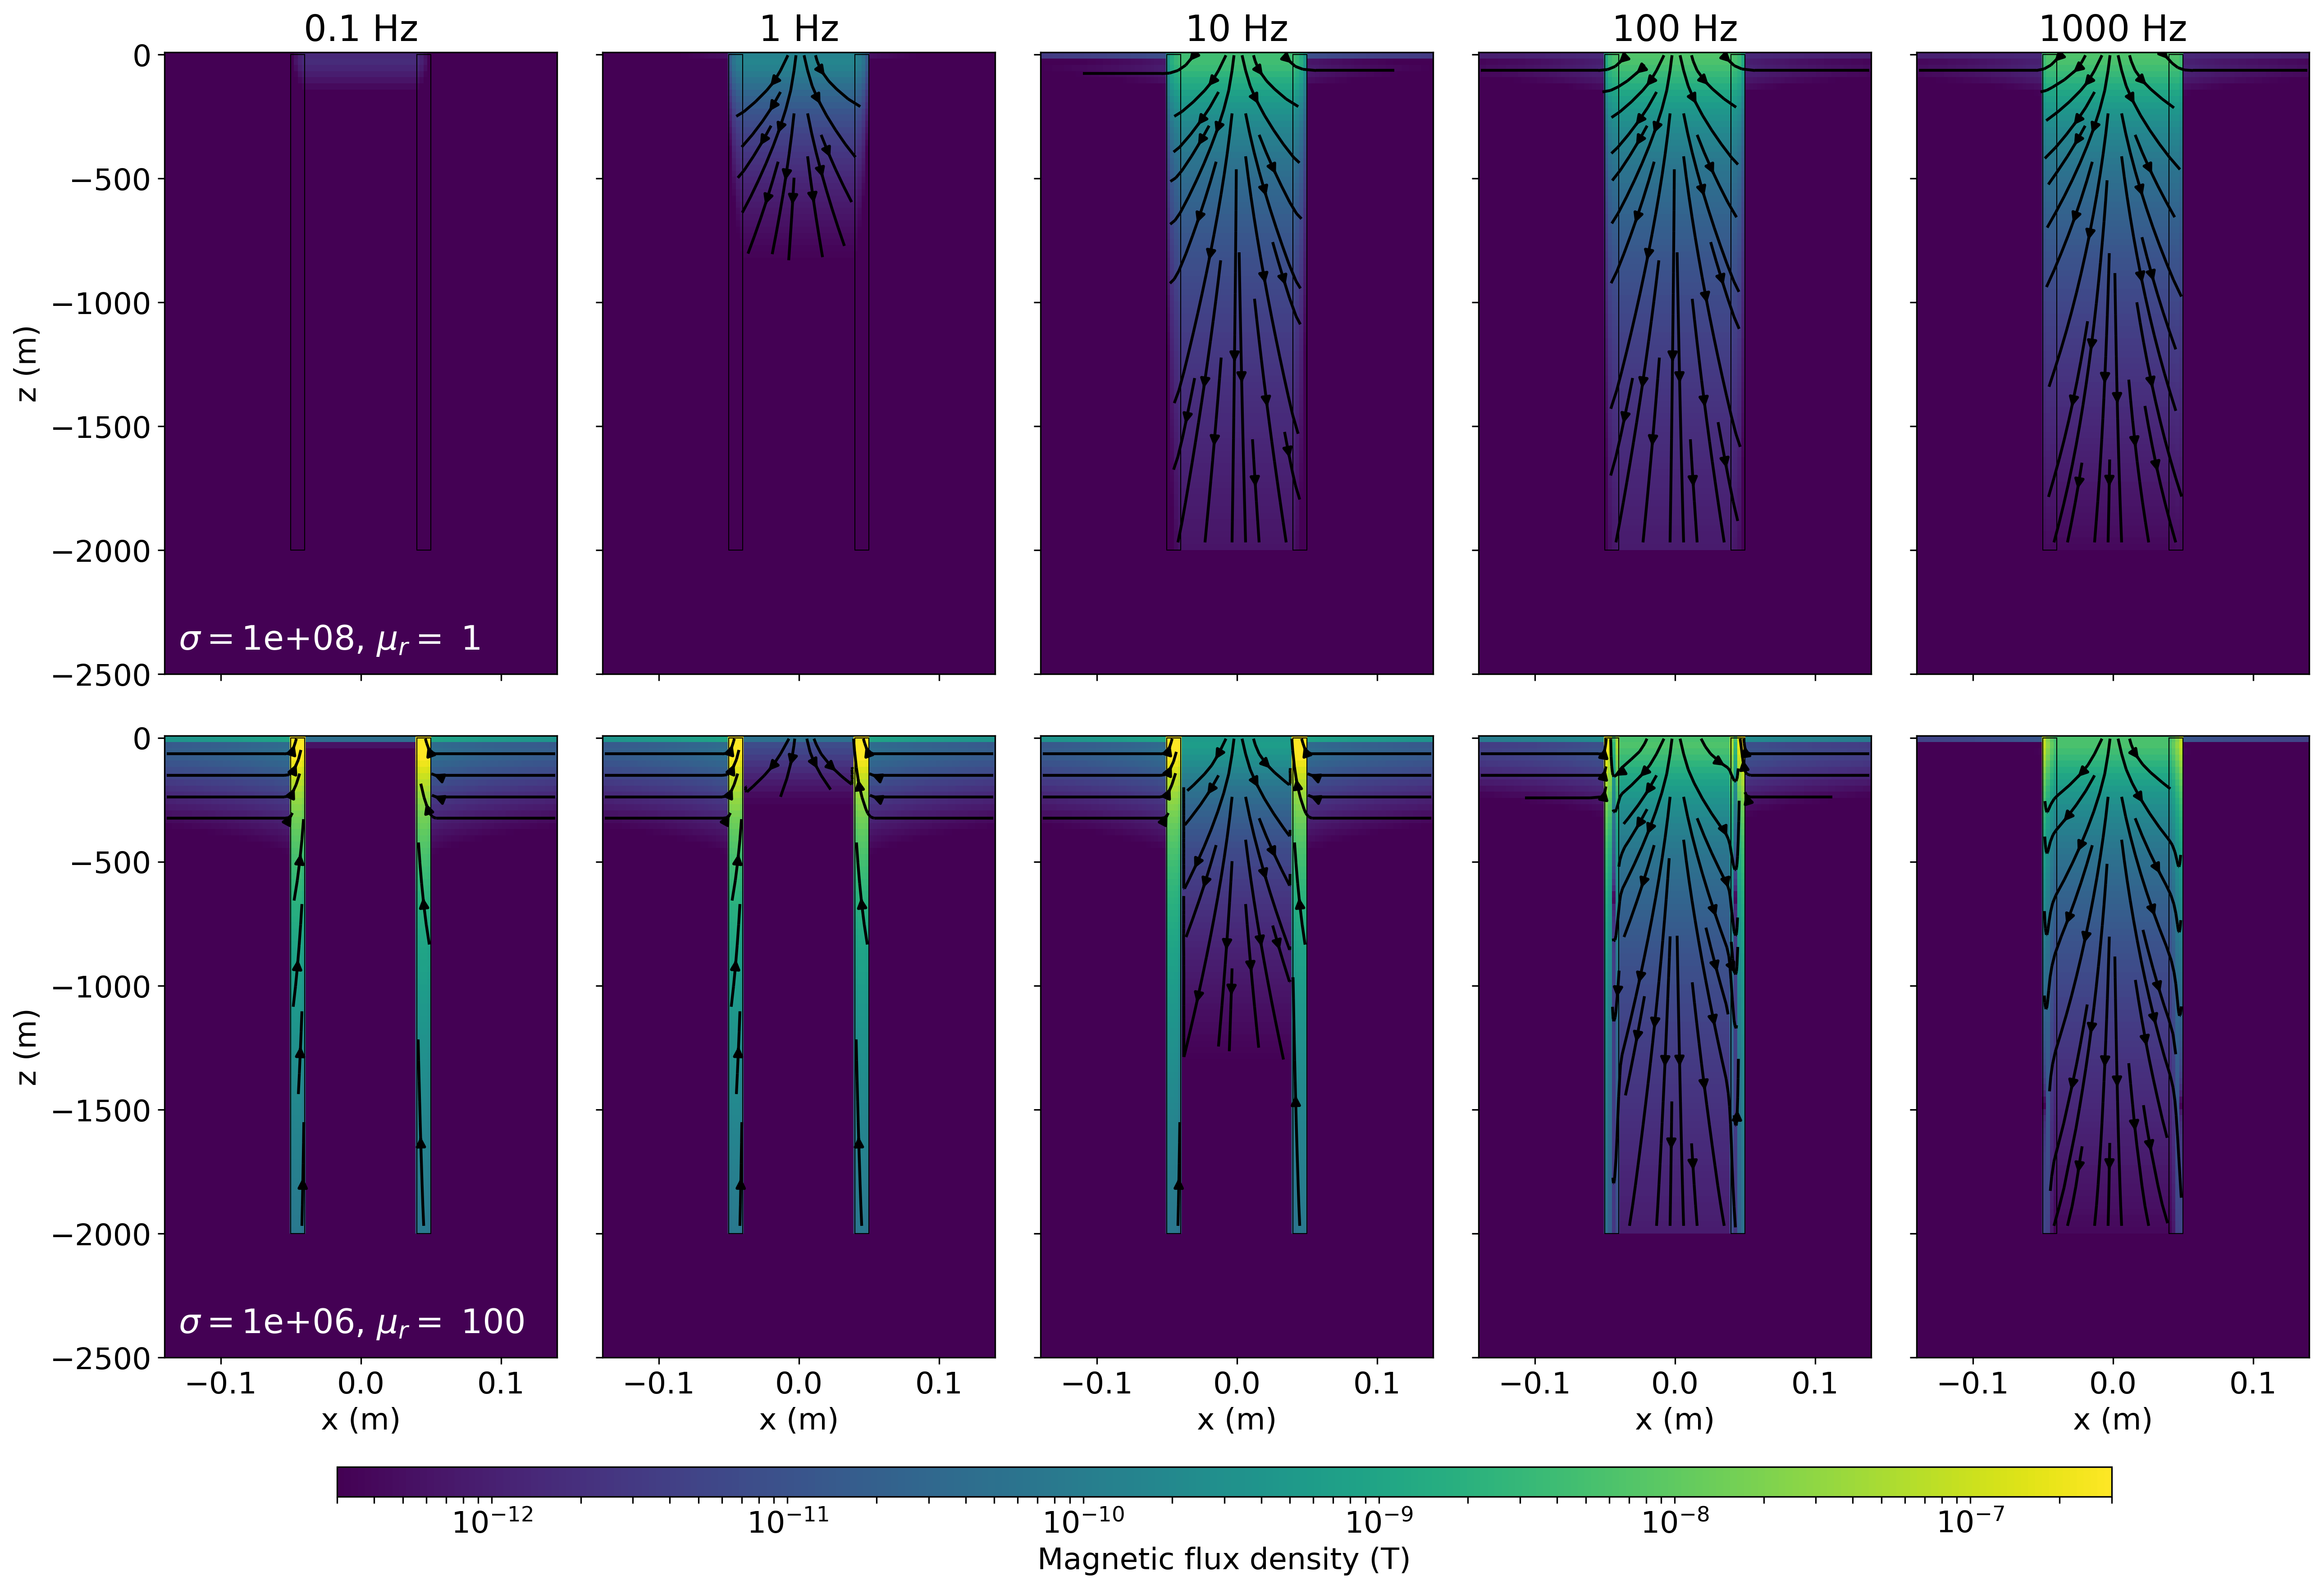
\includegraphics[width=\columnwidth]{figures/bfdem.png}
    \end{center}
\caption{
    Secondary magnetic flux density (with respect to a whole-space primary) at five different frequencies for a conductive pipe (top row)
    and for a conductive, permeable pipe (bottom row).
}
\label{fig:bfdem}
\end{figure}



Conducting a similar experiment in the time domain, we can compare the responses as a function of time. For this experiment, a step-off waveform is employed and data are measured after shut-off, the NSF is plotted in Figure \ref{fig:tdemNSF}. Note here that the secondary field is in the same direction as the primary, so after the source has been shut off, the secondary field is oriented upwards, as shown in Figure \ref{fig:btdem}. Shortly after shut-off, the rate of increase in the secondary field is the same for both the conductive and the conductive, permeable wells. A maximum normalized field strength of approximately 1 is reached for both cases. The responses begin to differ at $10^{-3}$ s where the conductive well maintains a NFS $\sim 1$ for approximately 1 ms longer than the permeable well before the fields decay away.


\begin{figure}[htb]
    \begin{center}
    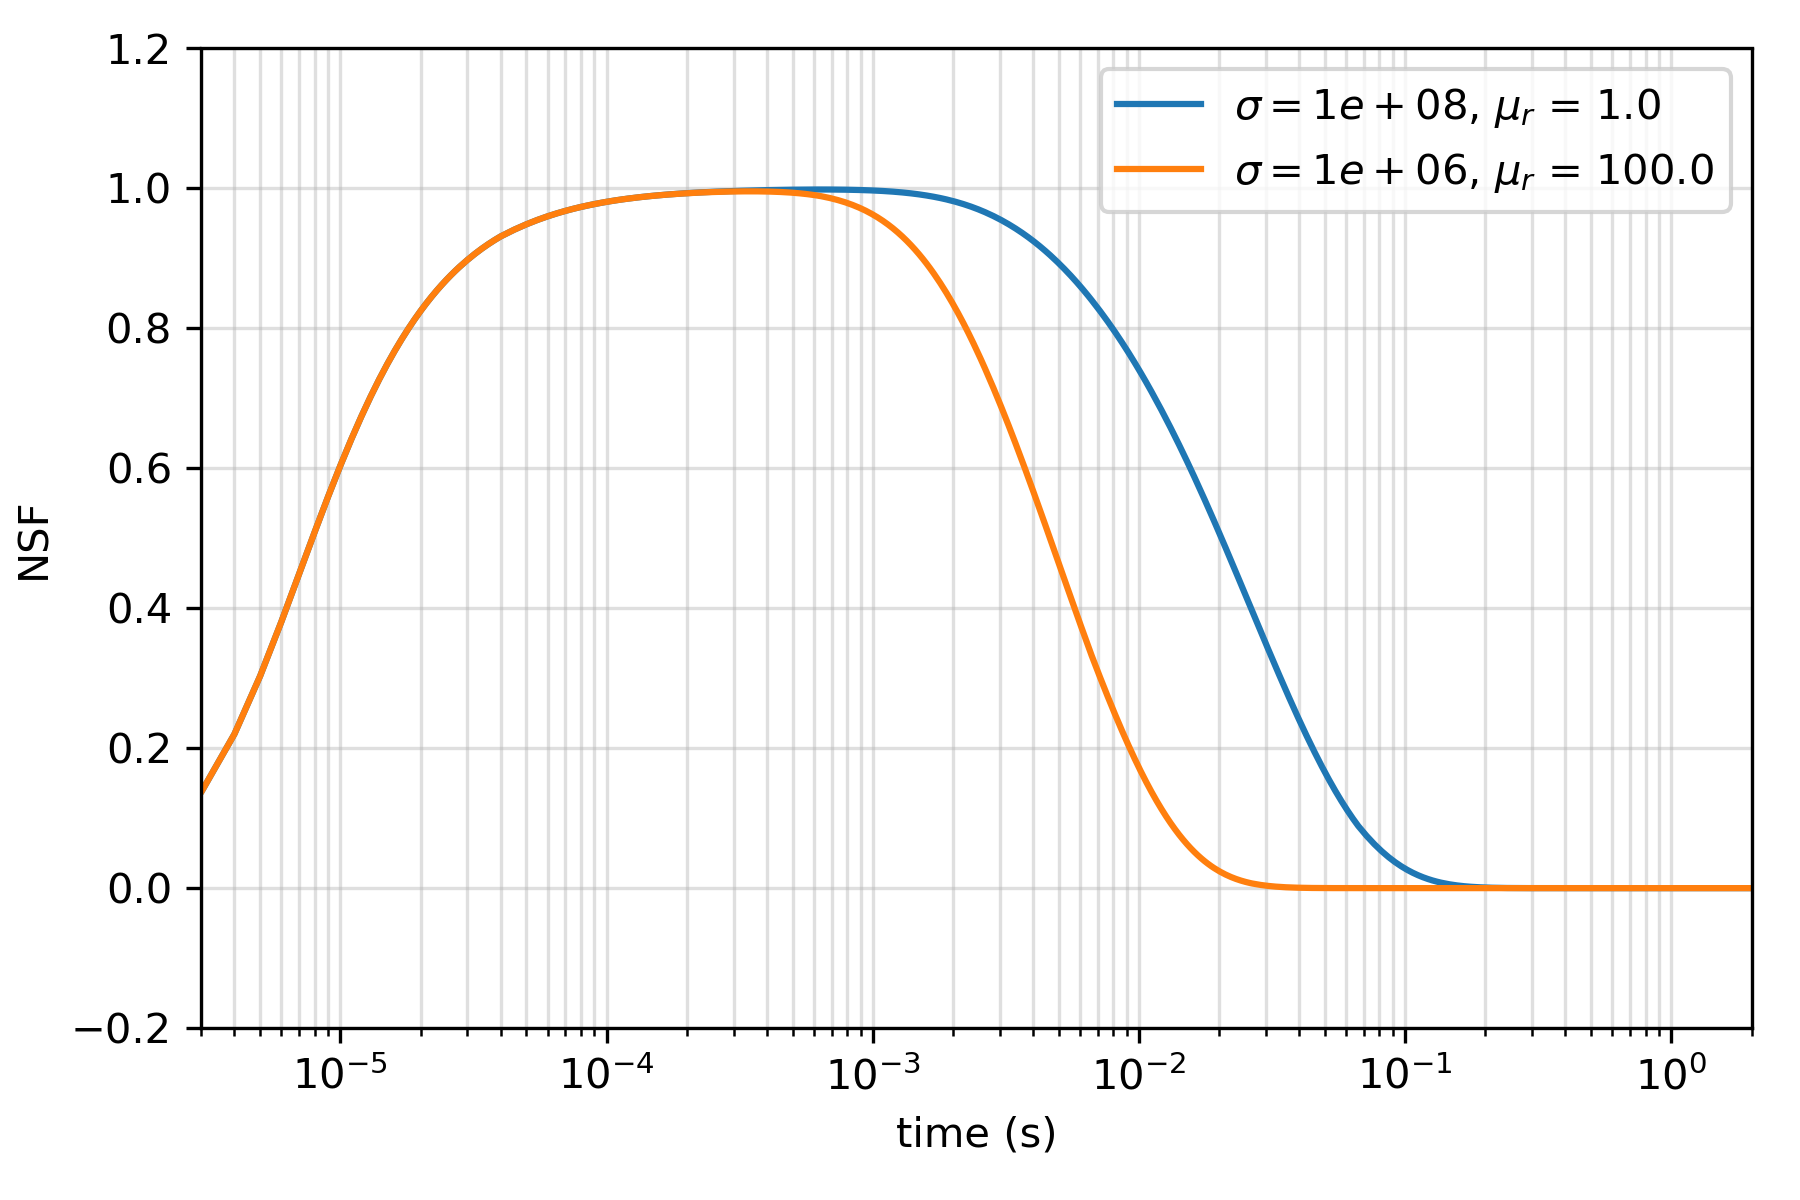
\includegraphics[width=0.6\columnwidth]{figures/tdemNSF.png}
    \end{center}
\caption{
    Normalized secondary field (NSF) through time.
    In the time-domain, we compute the NSF by taking the difference between the total magnetic flux at the reciever and the whole-space response
    and then taking the ratio with the whole-space magnetic flux prior to shutting off the transmitter.
}
\label{fig:tdemNSF}
\end{figure}



\begin{figure}
    \begin{center}
    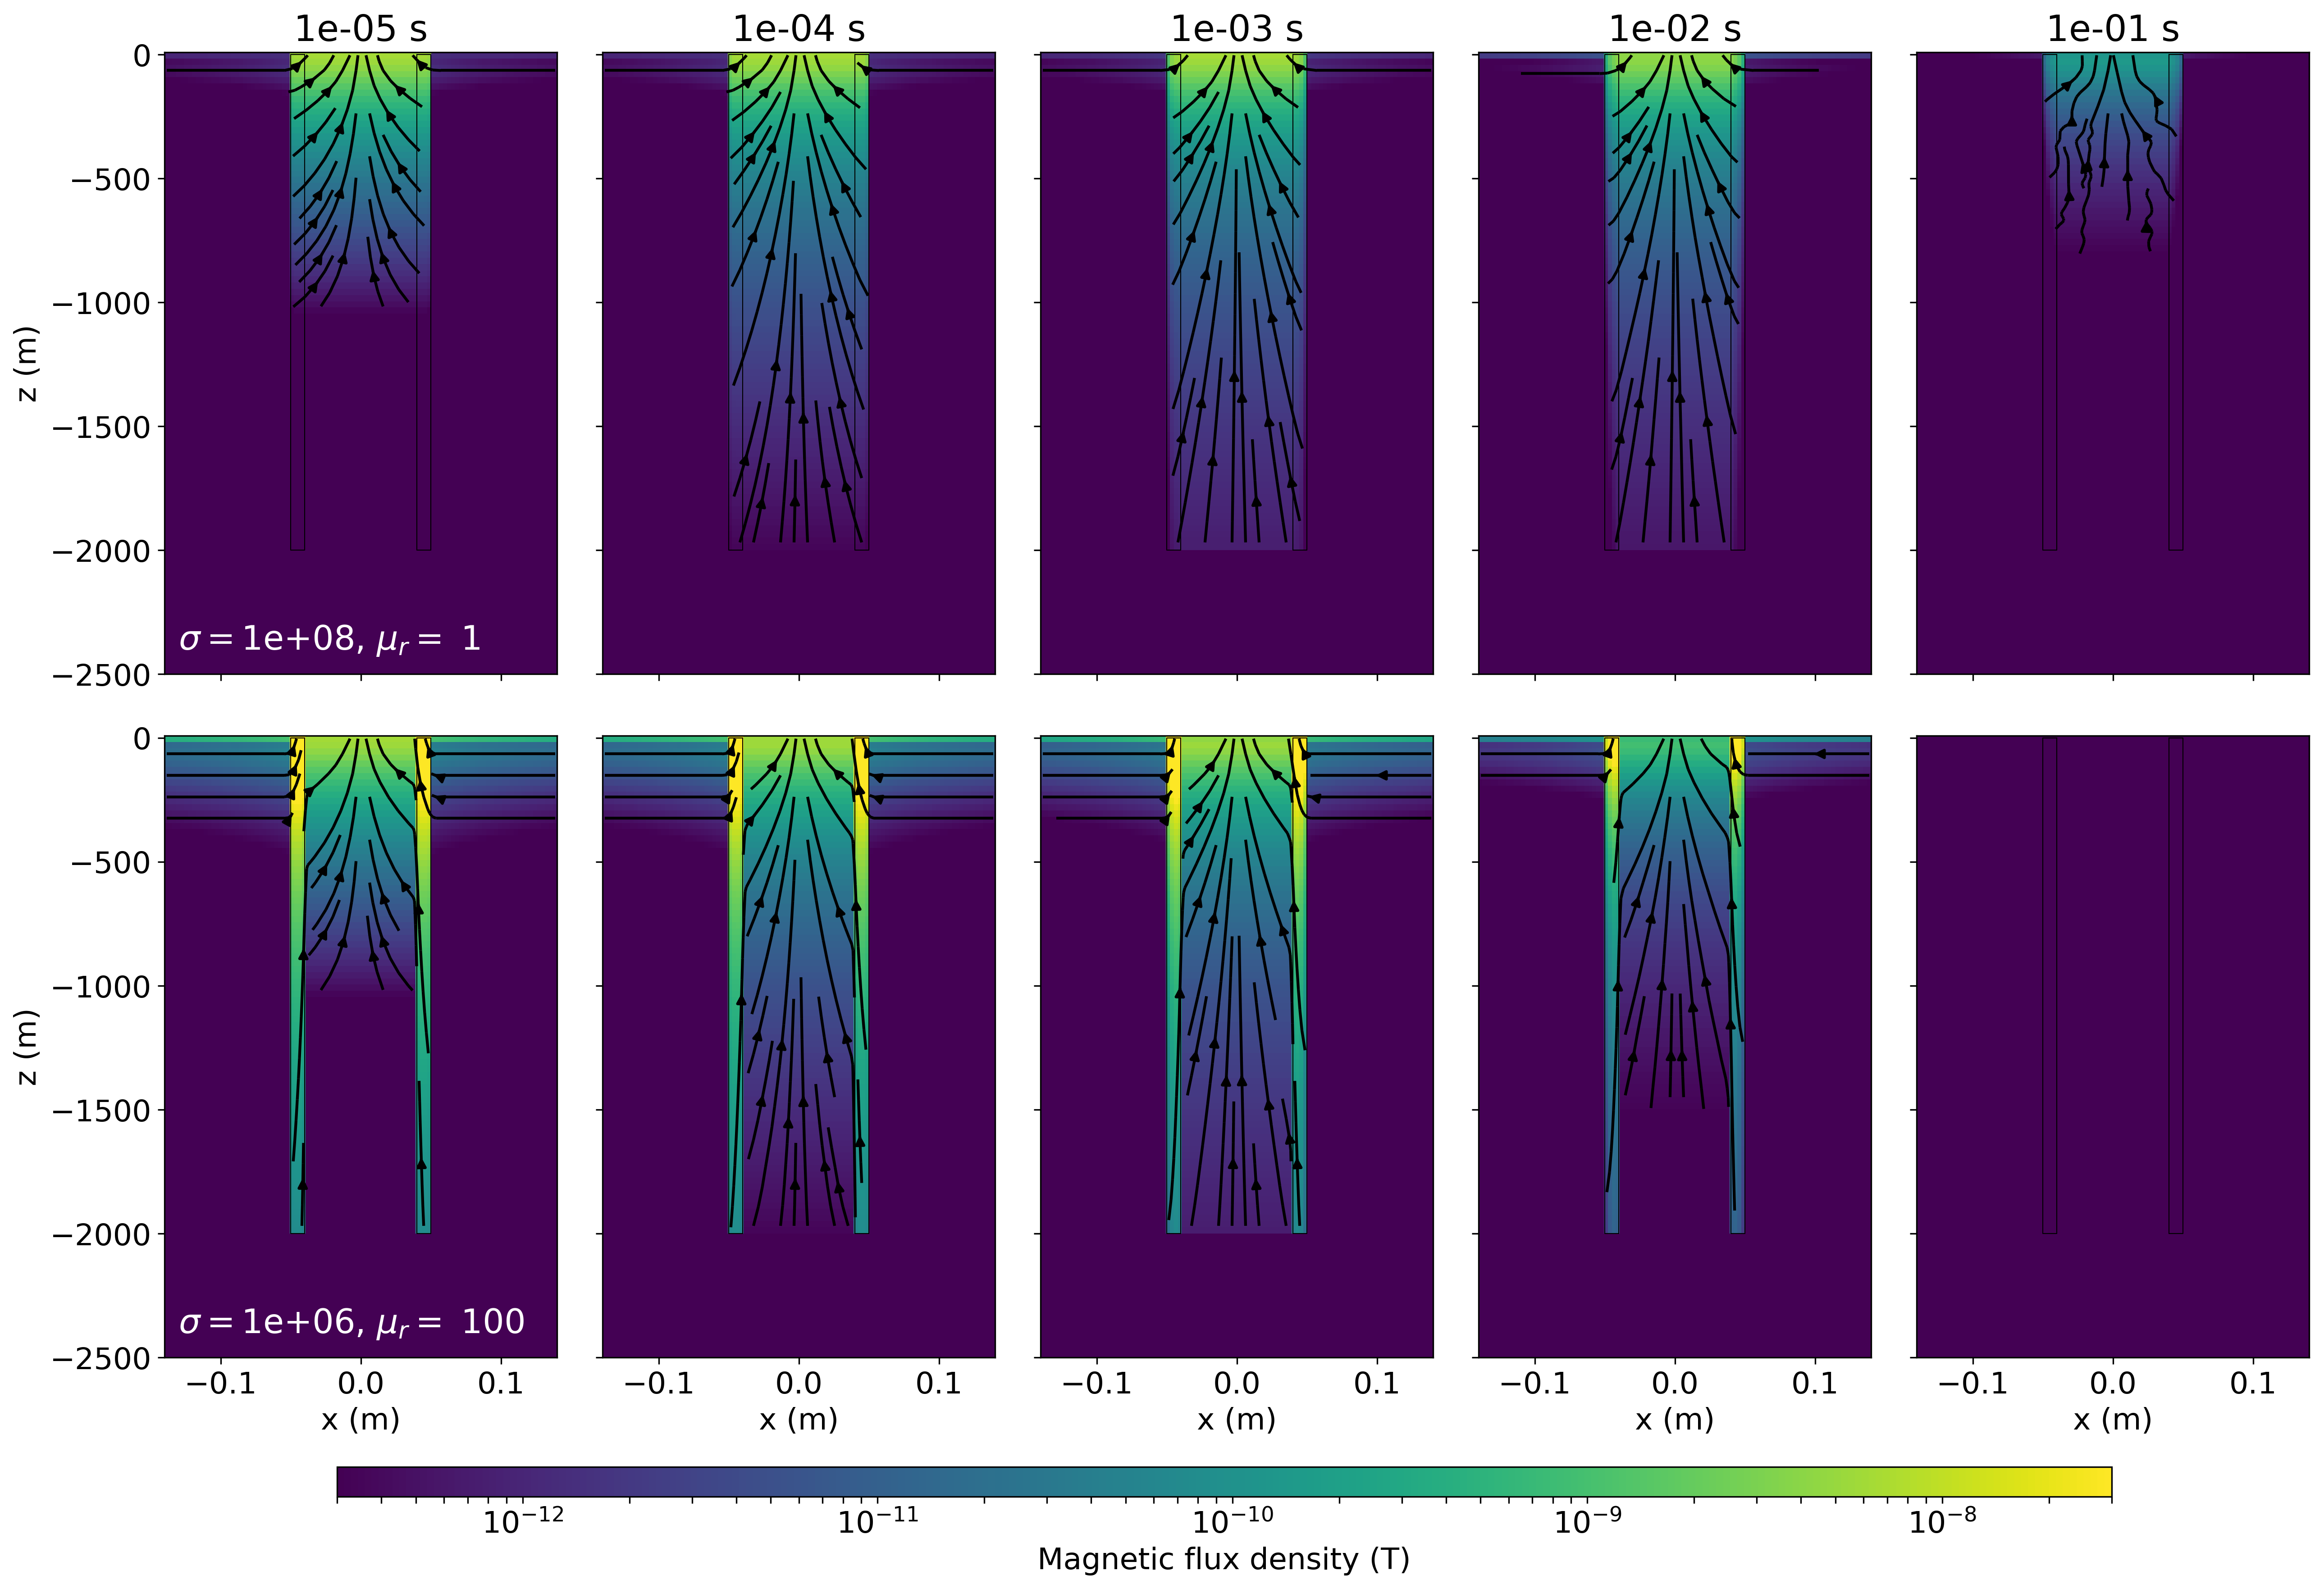
\includegraphics[width=\columnwidth]{figures/casing_software/btdem.png}
    \end{center}
\caption{
    Secondary magnetic flux density for a conductive well (top row) and a conductive, permeable well (bottom row) through time.
    The source waveform is a step-off waveform.
}
\label{fig:btdem}
\end{figure}



\subsubsection{Discussion}

It is important to note that although the product of the conductivity and permeability is identical for these wells, the geometry of the well and inducing fields results in different couplings for each of the parameters. For a vertical magnetic dipole source, the electric fields are purely rotational while the magnetic fields are primarily vertical. An approximation we can use to understand the implications of these geometric differences is to assume the inducing fields are uniform (e.g. the radius of the source loop is infinite) and to examine the conductance and permeance of the pipe. For rotational electric fields, the conductance is
\begin{equation}
    \mathcal{S} = \sigma \frac{t L}{2 \pi r}
    \label{eq:conductance}
\end{equation}

where $t$ is the thickness of the casing, $r$ is the radius of the casing and $L$ is the length-scale of the pipe segment contributing to the signal. For vertical magnetic fields, the permeance is
\begin{equation}
    \mathcal{P} = \mu \frac{ t 2 \pi r}{L}
    \label{eq:permeance}
\end{equation}

As the length-scale, $L$, is larger than the circumference of the pipe ($2\pi r$) the geometric contribution to the conductance is larger than that to the permeance.

An important take-away from this example is that the contributions of conductivity and permeability to the observed EM signals are not simply governed by their product. The geometry of the source fields plays an important role in how each contributes. Thus to accurately model conductive, permeable pipes, over a range of frequencies or times, a numerical code must allow both variable conductivity and variable permeability to be considered.

\section{Summary and Outlook}

I have developed software for solving Maxwell's equations on 2D and 3D cylindrical meshes. The medium can have variable electrical conductivity and magnetic permeability. The 2D solution is especially computationally efficient and has a large number of practical applications. When cylindrical symmetry is not valid, the 3D solution can be implemented; a judicious design of the mesh can often generate a problem with fewer cells than would be required with a tensor or OcTree mesh, thus reducing the computational cost of a simulation. I demonstrated the versatility of the codes by modelling the electromagnetic fields that result when a highly conductive and permeable casing is embedded in the earth.

I presented a number of different experiments involving DC, frequency-domain, and time-domain sources. The first two examples considered a simple DC resistivity experiment. In the first, I demonstrated that the numerically obtained currents, electric fields, and charges emulated those predicted by the asymptotic analysis in \cite{Kaufman1990} for long wells. The second example looked at the transition in behavior of currents and charges between short and long wells. Even in this relatively simple example, the physics was more complex than I originally anticipated; I had not intuitively expected to see the large increase in charge density that was observed near the ends of the well.

In the subsequent examples, I considered electromagnetic experiments and incorporated magnetic permeability in the simulations. I showed that for a conductive and permeable casing, excited by a circular current source, there is a complicated magnetic field that occurs in the top few centimeters of the pipe. Furthermore, the role of conductivity and permeability in the observed responses is more complex than their product; the source geometry and coupling with the casing are important to consider.

As new strategies and software are developed to handle more complex well-geometries, such as deviated or horizontal wells, it is important that we establish an understanding of the physics. Of critical importance is the ability to plot the charges, fields, and fluxes in the simulations. This is valuable for understanding the responses obtained from the experiment and it is a solid foundation for designing a field survey. I anticipate that the software provided with this thesis can be a resource for building understanding and additionally, serve as a tool for testing 3D simulations with boreholes present.

The software implementation is included as a part of the SimPEG ecosystem. SimPEG also includes finite volume simulations on 3D tensor and OcTree meshes as well as machinery for solving inverse problems. This means that the cylindrical codes can be readily connected to an inversion and additionally, simulations and inversions of more complex 3D geologic settings can be achieved by coupling the cylindrical simulation with a 3D tensor or OcTree mesh using a primary-secondary approach (e.g. example 3 in Appendix \ref{app:simpegem}). Beyond modelling steel cased wells, the 3D cylindrical mesh could prove to be useful in conducting 3D airborne EM inversions where a domain-decomposition approach, similar to that described in \cite{Yang2014}, is adopted.


%% The following is a directive for TeXShop to indicate the main file
%%!TEX root = ../../thesis.tex

\chapter{Direct current resistivity with steel-cased wells}
\label{ch:casing-dc}

\section{Introduction}

Subsurface resistivity can be a valuable part of a geologic interpretation, whether that be identifying lithologic units, characterizing changes within a reservoir, or imaging subsurface injections associated with carbon capture and storage or hydraulic fracturing. In many of these settings, steel-cased wellbores are present. Steel has a significant electrical conductivity, which is generally six or more orders of magnitude larger that of the surrounding of the geologic formation. Clearly, such a large contrast is important to consider when conducting a direct current (DC) resistivity survey. On one-hand, the role of the steel casing may be viewed as ``distortion'' which complicates the signals of interest \citep{Wait1983, Holladay1984, Johnston1987}. In other scenarios, a wellbore may be beneficial in that it can serve as an ``extended electrode'' so that current-injection and sampling of the resultant electrical potentials can take place beneath near-surface heterogeneities \citep{Ramirez1996, Rucker2010, Rucker2012, Ronczka2015} or so that currents injected at the surface can reach significant depths \citep{Schenkel1994, Weiss2016, hoversten2017borehole}. The use of casings as extended electrodes extends back several decades. \cite{Sill1978} used the well casing as a buried electrode for their mis-\`a-la-masse experiment at the Roosevelt Hot Springs geothermal field in Utah, as did \cite{osti_6375177} for their mis-\`a-la-masse mapping of a high temperature geothermal reservoir in Hawaii. Sill (1983) used the well as a source to monitor an injection test at Raft River, Idaho to determine if measurable changes that might indicate the direction of fluid flow could be observed. \cite{Rocroi1985} delineated a known resistive hydrocarbon deposit in the USSR by injecting current into two cased wells. More recently, applications for hydraulic fracturing, enhanced oil recovery and carbon capture and storage have been of much interest \citep{Commer2015, Um2015, Weiss2016, hoversten2017borehole}.

To build a physical understanding of electrical and electromagnetic methods in settings where steel-cased wells are present, there are several areas to be investigated. First, the significant conductivity of the steel will impact the behavior of the charges, currents, and electric fields. This is true at the electrostatic limit, relevant to DC resistivity surveys, as well as when the source fields are time-varying, as in electromagnetic (EM) surveys. When considering EM surveys, induction effects also influence the responses, and magnetic fields and fluxes become relevant, meaning that the magnetic permeability of the steel then introduces further complexity into the signals we measure. This chapter is concerned with the first set of physical phenomena: understanding the physics of steel casings at DC.

Much of the initial theory and understanding of the behavior of electric fields, currents, and charges, was developed in the context of well-logging. \cite{Kaufman1990} and \cite{Kaufman1993} provide a theoretical basis for our understanding; the first paper derives an analytical solution for a DC experiment where an electrode is positioned along the axis of an infinite length well, and discusses where charges accumulate and how currents leak into the surrounding formation. From this, \cite{Kaufman1990} shows that by measuring the second derivative of the electric potential, information about the formation resistivity can be obtained. The second paper extends the analysis for finite length wells. \cite{Schenkel1990, Schenkel1991, Schenkel1994} pioneered numerical work analyzing the influence of steel-cased wells on geophysical data using an integral equation approach for solving the DC resistivity problem. They expand upon the logging-through-casing application and discuss limitations of the transmission line solution presented in \cite{Kaufman1990} for this application. They also explored the feasibility of cross-hole and borehole-to-surface surveys where one electrode is placed within, or beneath, a cased borehole. These examples demonstrated that the casing can improve detectability of a conductive target as compared to the scenario where no cased well is present.

In this chapter, I focus on three aspects of DC resistivity in the presence of steel-cased well. In section \ref{sec:casing_integrity}, I examine the feasibility of conducting a surface DC survey to detect a flaw in the casing and discuss factors that influence detectability of a flaw. In section \ref{sec:survey_design}, I examine the use of DC resistivity for geophysical imaging when a steel-cased well is present. Finally, in section \ref{sec:approximating_wells}, I assess strategies applied in the literature for approximating a steel-cased well with a coarse-scale model to reduce computational cost.

Source codes for all of the simulations shown are open source, licensed under the MIT license, and are available as Jupyter notebooks (see Appendix \ref{app:code_list}). The examples in the paper have been selected with an emphasis on examining physical principles; however, I envision that the Jupyter notebooks included with this chapter could serve as useful survey design tools.
\section{DC resistivity for casing integrity}
\label{sec:casing_integrity}

Degraded or impaired wells can pose environmental and public-health hazards. A flaw in the cement or casing can provide a conduit for methane to migrate from depth into groundwater aquifers or into the atmosphere. This is particularly of concern for shale gas wells. Elevated levels of thermogenic methane, which are attributed to deep sources (rather than biogenic methane which can be generated closer to the surface), in groundwater wells in Pennsylvania has been positively correlated with proximity to shale gas wells in the Marcellus and Utica \citep{Osborn2011, Jackson2013}, and failure rates of unconventional wells (e.g. shale gas wells) is estimated to be 1.57 times larger than that of a conventional well drilled in the same time-period \citep{Ingraffea2014}. Wells can fail if there is a compromise in the cement or the casing. To diagnose the integrity of a well with electrical methods, we require a contrast in electrical conductivity to be associated with the flaw, thus I will focus attention to detecting flaws in the highly conductive casing.

Under what circumstances should we be able to detect a flaw in the casing using DC resistivity from the surface? To address this question, I begin by examining how a flaw which comprises the entire circumference of the pipe along some depth interval changes the charge distribution and thus the resultant electric fields we measure on the surface. From there, I investigate the role of parameters including the depth of the flaw and the background conductivity on our ability to detect it from the surface. Finally, I examine the scenario in which only a portion of the circumference of the pipe is flawed.

\subsection{Basic experiment}

The experiment I consider is a ``top-casing'' DC resistivity experiment where one electrode is connected to the wellbore at the surface and a return electrode is positioned some distance away. The concept and basic physics is the same as a mis-\`a-la-masse survey in which the positive electrode is connected to a conductive target. When the source is turned on, positive charges are distributed on the interface between the conductive target and the resistive host. Electric potentials are measured on the surface and these data are then used to infer information about the extent of the conductor \citep{Telford1990}. Applying the same principles to a casing integrity experiment, I connect a positive electrode to the casing, and for an intact casing, positive charges will be distributed on the outer interface of the casing along its entire length. If corrosion causes a flaw across the diameter of the casing, the continuity of the conductive flow-path for charges is interrupted, thus we expect a larger charge on the top portion of the flawed casing than we would if it were intact. This results in a larger electric field at the surface than would be observed if the casing were intact. The difference in electric field (or electric potentials) from the expected electric field that results from an intact well could then be an indicator that there is a problem with the well.

To demonstrate the principles, I start by considering a simple model of a casing in a half-space. The intact well is 1 km long, has an outer diameter of 10 cm, a thickness of 1 cm and a conductivity of $5\times10^6$ S/m. The background is $10^{-1}$ S/m, and the conductivity of the inside of the well is taken to be equal to that of the background. The positive electrode is connected to the top of the casing and the return electrode is positioned 2 km away. To simulate the physics, the 3D cylindrical DC code described in Chapter \ref{ch:casing-software} was employed. In Figure \ref{fig:casing_integrity_basics} I show cross-sections of the: (a) electrical conductivity model, (b) current density, (c) charge density, and (d) electric field for the intact well (top row)  and a flawed well (bottom row) that contains a 10 m gap in the casing at 500 m depth. As expected, the introduction of a resistive flaw prevents currents from reaching the bottom portion of the well. This results in increased currents, charge density and thus electric fields within the top 500 m.
\begin{figure}
    \begin{center}
    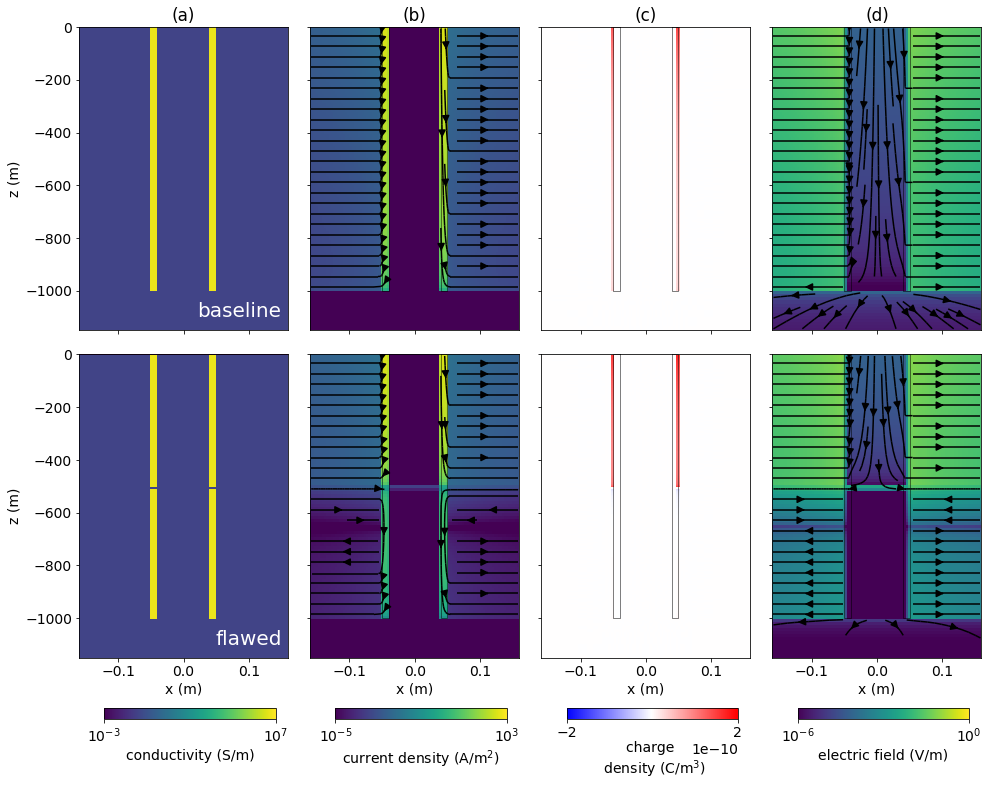
\includegraphics[width=0.8\textwidth]{figures/dc_casing/casing_integrity_basics.png}
    \end{center}
\caption{
    Cross section showing: (a) electrical conductivity, (b) current density, (c) charge density, and (d) electric field
    for a top-casing DC resistivity experiment over (top) an intact 1000m long well and (bottom) a 1000m long well
    with a 10m flaw at 500m depth.
}
\label{fig:casing_integrity_basics}
\end{figure}


To quantify the charge along the length of the well, I have plotted the charge as a function of depth for the intact well (black), flawed well (blue), and also a short well of 500 m length (grey dash-dot) in Figure \ref{fig:casing_charge}a. In each of the wells, we observe that there is an increase in charge density near the end of the discontinuity along the length of the well. This was also noted in \cite{Griffiths1997} and in Chapter \ref{ch:casing-software} -- this behavior is attributed to edge effects. At an interface between materials with two different conductivities, the normal component of the current density must be conserved, as well as the tangential component of the electric field; the discontinuity at the end of the pipe, and at the location of the flaw, means the continuity conditions must be preserved simultaneously in the radial and vertical directions, and this complicates the behavior of the fields, fluxes and charges. Another observation is that the flawed and short wells have nearly identical charge distributions in the top 500 m. In the bottom portion of the flawed well, where the remaining conductive material is, a small dipolar charge is introduced, but this is nearly an order of magnitude smaller than the charge in the top portion of the pipe. The signal due to the flaw can be defined as the difference between the total response due to a flawed well and the total response due to an intact well (the primary); I  will refer to this difference as the secondary response. The secondary charge is dipolar in nature with positive charge above the flaw and negative charge beneath the flaw. Note that the charge distributions along the short well, truncated where the flaw starts at 500 m depth, and along the top portion of the flawed well are almost identical; these charges are the source of signal for a surface electric field measurement. This suggests that an inversion strategy, where one attempts to estimate the length of a well, may be an effective approach for characterizing the depth to a flaw.


\begin{figure}
    \begin{center}
    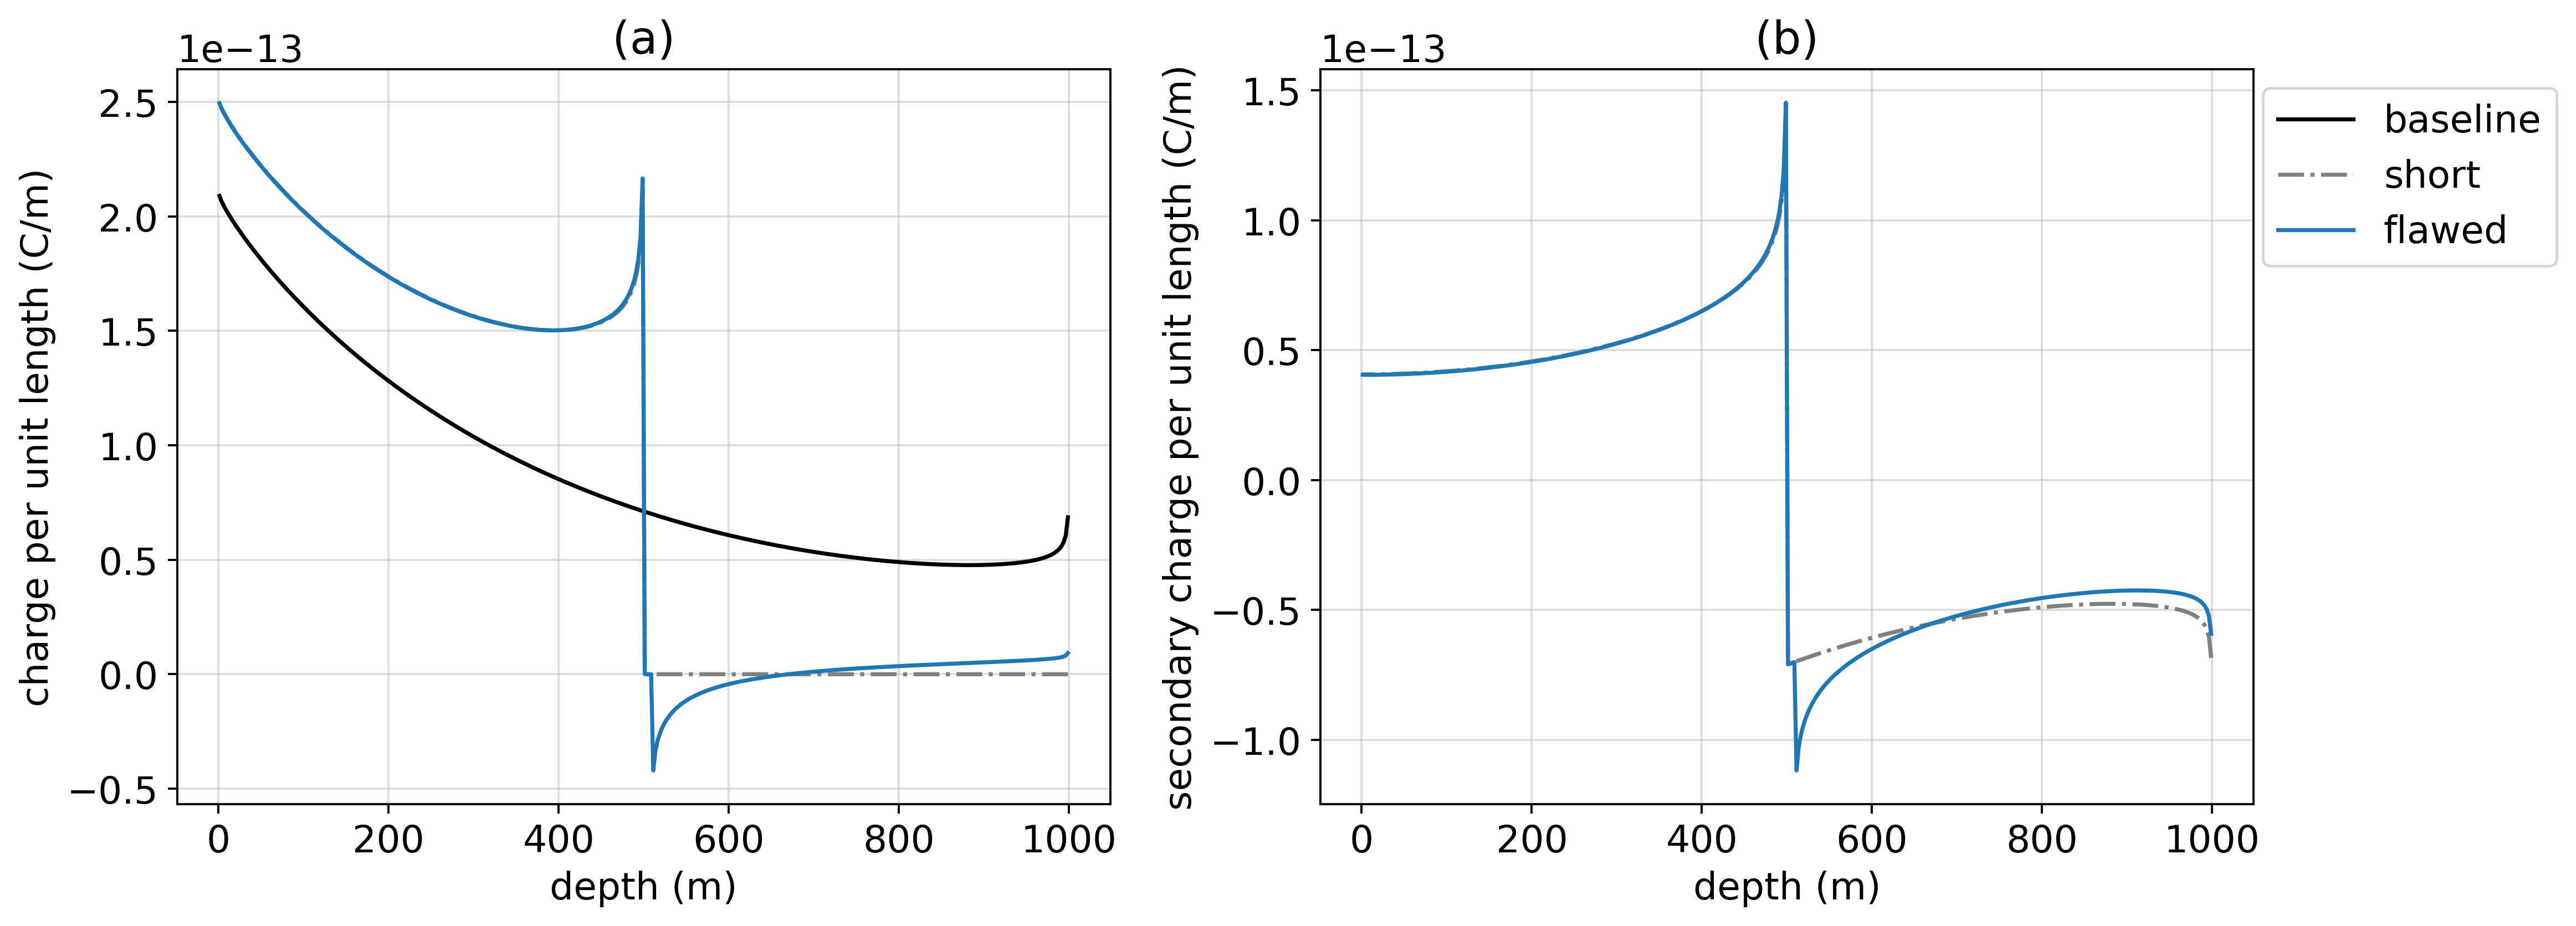
\includegraphics[width=\textwidth]{figures/casing_charge.png}
    \end{center}
\caption{
    (a) Charge along the length of the intact well (black),
    a 500m well ( ``short'', grey dash-dot), and
    a well with a 10m flaw at 500m depth (blue),
    in a top-casing DC resistivity experiment.
    (b) Secondary charge along the flawed and short wells. The primary is
    defined as the electric field due to the 1000m long intact well. The return electrode
    is 2000m away from the well.
}
\label{fig:casing_charge}
\end{figure}


\subsubsection{Impact of the vertical extent of the flaw}

A 10 m flaw is quite long and it is of interest to see how the results are changed if the flaw has a smaller vertical extent. The distribution of charges shown in Figure \ref{fig:casing_charge} hints that the flaw may not need to be very long in order to still significantly influence the response. To confirm this, I adopt a much finer vertical discretization in order to model smaller flaws. Here, I use a shorter, 50 m long well in order to reduce computational load. The flaw is positioned at 25 m depth, and the length of the impairment is varied. This simulation is conducted on a cylindrically symmetric mesh, the positive electrode is connected to the casing, and a return electrode is positioned 50 m away.

The resultant charge distributions are shown in Figure \ref{fig:casing_charge_flawdz}. For comparison, I again show the charge on a well that is truncated at the location of the flaw; this is the  ``short'' well and results are displayed using the grey dash-dot line. The charge distribution is similar for all of the flawed-well scenarios, even for flaws smaller than the thickness of the casing ($10^{-2}$ m). We see similar behavior to that shown in Figure \ref{fig:casing_charge}, where positive charge accumulates within the top portion of the well and a small dipole charge is present in the bottom portion of the well. There are minor differences in amplitude as the vertical extent of the flaw is changed; as the extent of the flaw decreases, the amplitude of the dipolar charge on the bottom portion of the well increases slightly while the amplitude of the positive charge on the top portion of the well decreases. These distinctions, however, are small in magnitude, and even if the background is more conductive, the casing is still orders-of-magnitude larger in conductivity than any geologic material we are likely to encounter. Thus, I conclude that, so long as the impairment affects the entire circumference of the casing, the extent of that flaw has little impact on the charge that accumulates in the top portion of the well. As such, I will proceed in our analysis using a 10 m flaw in the 1 km well so that a fine vertical discretization is not necessary.

\begin{figure}
    \begin{center}
    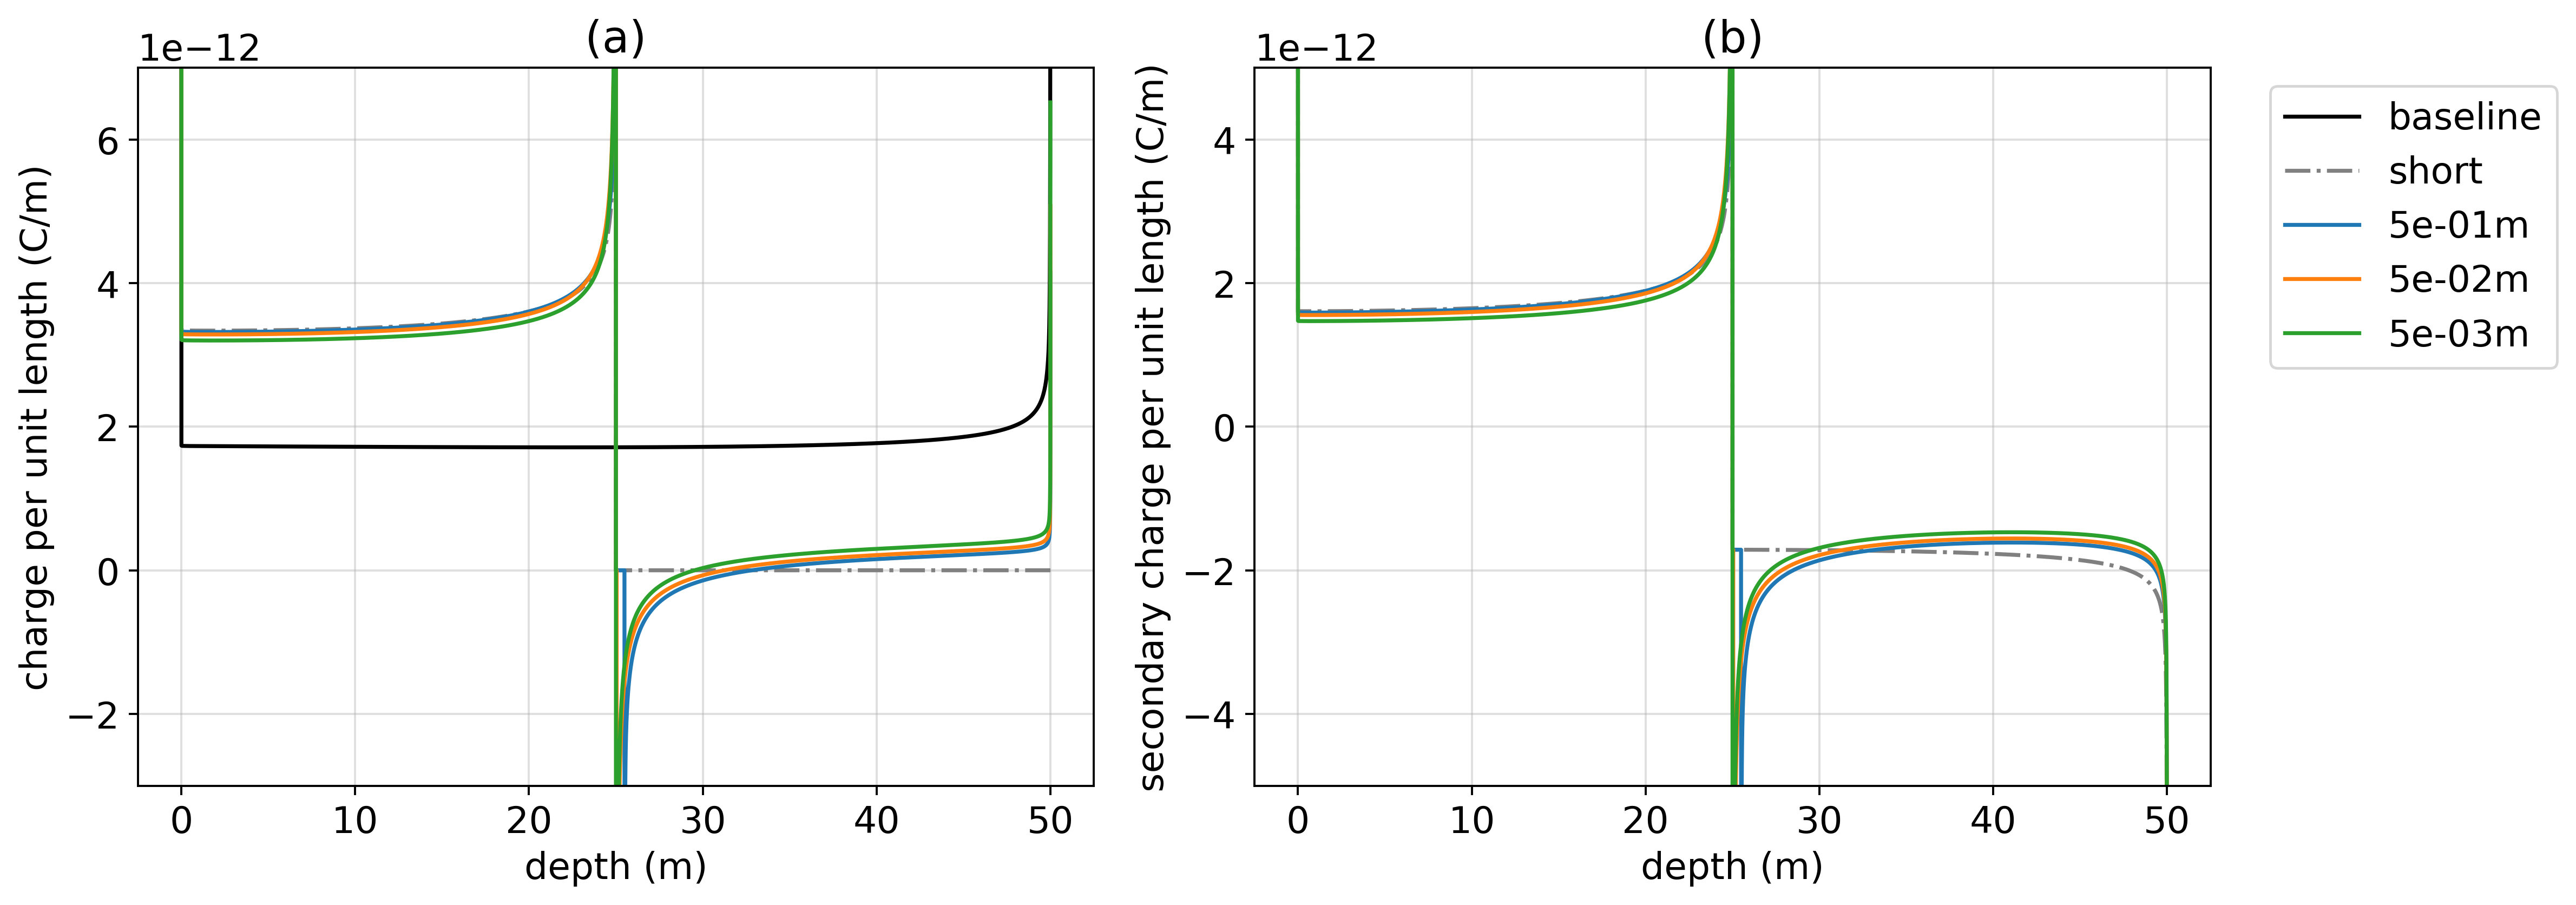
\includegraphics[width=\textwidth]{figures/casing_charge_flawdz.png}
    \end{center}
\caption{
    (a) Charge along the length of a 50m long intact well (black),
    a 25m well (``short'', grey dash-dot), and four wells, each with a flaw
    starting at 25m depth and extending the length indicated by the legend
    ($5 \times 10^{-1}$ m (blue), $5 \times 10^{-2}$ m (orange), and $5 \times 10^{-3}$ m (green))
    in a top-casing DC resistivity experiment.
    For reference, the diameter of the casing is $10^{-1}$ m and its thickness is $10^{-2}$ m.
    (b) Secondary charge along the flawed and short wells. The primary is
    the baseline in (a). The return electrode
    is 50m away from the well and a cylindrically symmetric mesh was used in the simulation.
}
\label{fig:casing_charge_flawdz}
\end{figure}



\subsection{Survey design considerations}

When examining detectability of a signal, there are two aspects to consider: (1) the signal must be larger than the noise floor of the instrument, and (2) the signal must be a significant percentage of the primary; for the casing integrity experiment, the primary is the signal due to the intact well. Due to the cylindrical symmetry of the charge on the well, we expect the electric field at the surface to be purely radial, thus only radial electric field data need be collected at the surface.

In Figure \ref{fig:integrity_e_fields}, I have plotted the primary field (top row), secondary field (second row) and secondary field as a percentage of the primary (third row) for four different return electrode locations. In (a), the return electrode is 2000 m offset from the well, in (b) the offset is 750 m, in (c) the offset is 500 m, and in (d) the offset is 250 m. In addition to the plan view, I have plotted the primary electric field (black),  total electric field for the flawed well (blue) and secondary radial electric field (orange) along the $\theta = 90^\circ$ azimuth in the fourth row of Figure \ref{fig:integrity_e_fields}. The fifth row shows the secondary as a percentage of the primary.




\begin{figure}
    \begin{center}
    \includegraphics[width=0.9\textwidth]{figures/dc_casing/integrity_e_fields.png}
    \end{center}
\caption{
    (Top row) primary electric field, (second row) secondary electric field,
    and (third row) secondary electric field as a percentage of the primary radial electric field
    for a return electrode that is offset (a) 2000m, (b) 750m, (c) 500m, and (d) 250m
    from the well. The primary is defined as the response due to the 1000m
    long, intact well. Electrode locations are denoted by
    the red dots. In the third row, the colorbar has been limited
    between 20\% and 100\%. The fourth and fifth rows show radial electric field data
    collected along the $\theta=90^\circ$ azimuth (white dotted lines in
    the top three rows). The fourth row shows the primary (black line), the total
    electric field due to the flawed well (blue line), and the secondary
    radial electric field (orange line). The fifth row shows the secondary as a
    percentage of the primary.
}
\label{fig:integrity_e_fields}
\end{figure}


At the furthest offset (Figure \ref{fig:integrity_e_fields}a), there is nearly complete cylindrical symmetry in the primary field. With complete cylindrical symmetry there is no preferential direction along which to collect data. As I move the return electrode closer, for example to 750 m from the well, we notice that the secondary electric field does not change substantially. However, if I examine the ratio of the secondary to the primary (second and fifth rows), we see that the ratio has increased. Although the primary field has similar, if not larger amplitude near the well, it also has considerable curvature. As a result, the proportion of the primary field that is in the radial direction has decreased in amplitude. Hence the important characteristic, the ratio of the secondary to primary of the radial components, has increased. The above principles are further enhanced as the return current is brought closer to the well as in panels (c) and (d), where the return electrode is brought to 500 m and 250 m from the well.  Again, for all of these examples the amplitude of the secondary field at the surface is quite similar. However, the choice of azimuth for the survey line will greatly affect the size of the ratio. In terms of survey design, we can take advantage of the return electrode to reduce coupling with the primary.

For our following examples I will place the return electrode at 500 m from the well and collect radial data along a line that is perpendicular to the source line. I will examine several factors influencing detectability of a flaw, including the depth of the flaw and the conductivity of the background in the following sections. I will also examine the scenario where only a portion of the circumference of the well has been compromised.


\subsection{Factors influencing detectability}
\subsubsection{Depth of the flaw}
The introduction of a flaw in the well changes the distribution of charges along the length of the well and causes a secondary dipolar charge centered about the flaw. The position and strength of this dipole will affect our ability to detect the flaw. To examine this, I have taken the same model of a 1km pipe in a $10^{-1}$ S/m background and varied the depth of the flaw from 300 m to 900 m. In Figure \ref{fig:integrity_depth}, I plot radial electric field results along a line perpendicular to the source electrodes; the return electrode is positioned 500 m from the well. In (a), I show total radial electric field, in (b) the secondary radial electric field (with the primary being the electric field resulting from the intact well, shown in black in panel a), and in (c) I show the secondary radial electric field as a percentage of the primary. I have also indicated where values fall below a $10^{-7}$ V/m noise floor on Figure \ref{fig:integrity_depth} (a) and (b), as well as those that fall below a 20\% threshold in (c). A threshold of 20\% may be conservative, however, it does depend on knowledge of the background conductivity as well as the geometry and physical properties of the well. In many scenarios, these may not be well-constrained, thus I select a conservative threshold for this analysis. Any detectability analysis will be site-dependent and I have therefore made all source-code available so that a similar workflow may be followed and adapted to include setting-specific parameters.

When a well is impaired, the total radial electric field is larger than that due to the baseline, intact well. The strength of the secondary response decreases as the depth of the flaw increases. For this example of a 1000 m long well in a $10^{-2}$ S/m background, a flaw at 900 m depth is not detectable; there is no overlap between the region in which the secondary electric field (Figure \ref{fig:integrity_depth}b) is above the noise floor and the region in which the secondary comprises a significant percentage of the primary (Figure \ref{fig:integrity_depth}c). This might be expected, as the difference between the charges distributed along a 900 m long segment versus the 1000 m long well are not drastically different. For a flaw at 700 m depth, there is a window between 400 m offset and 800 m offset over which the radial electric field data are sensitive to the flaw. As the depth to the impairment decreases, both the spatial extent over which data are sensitive to the flaw, and the magnitude of the secondary response in those data, increase.



\begin{figure}
    \begin{center}
    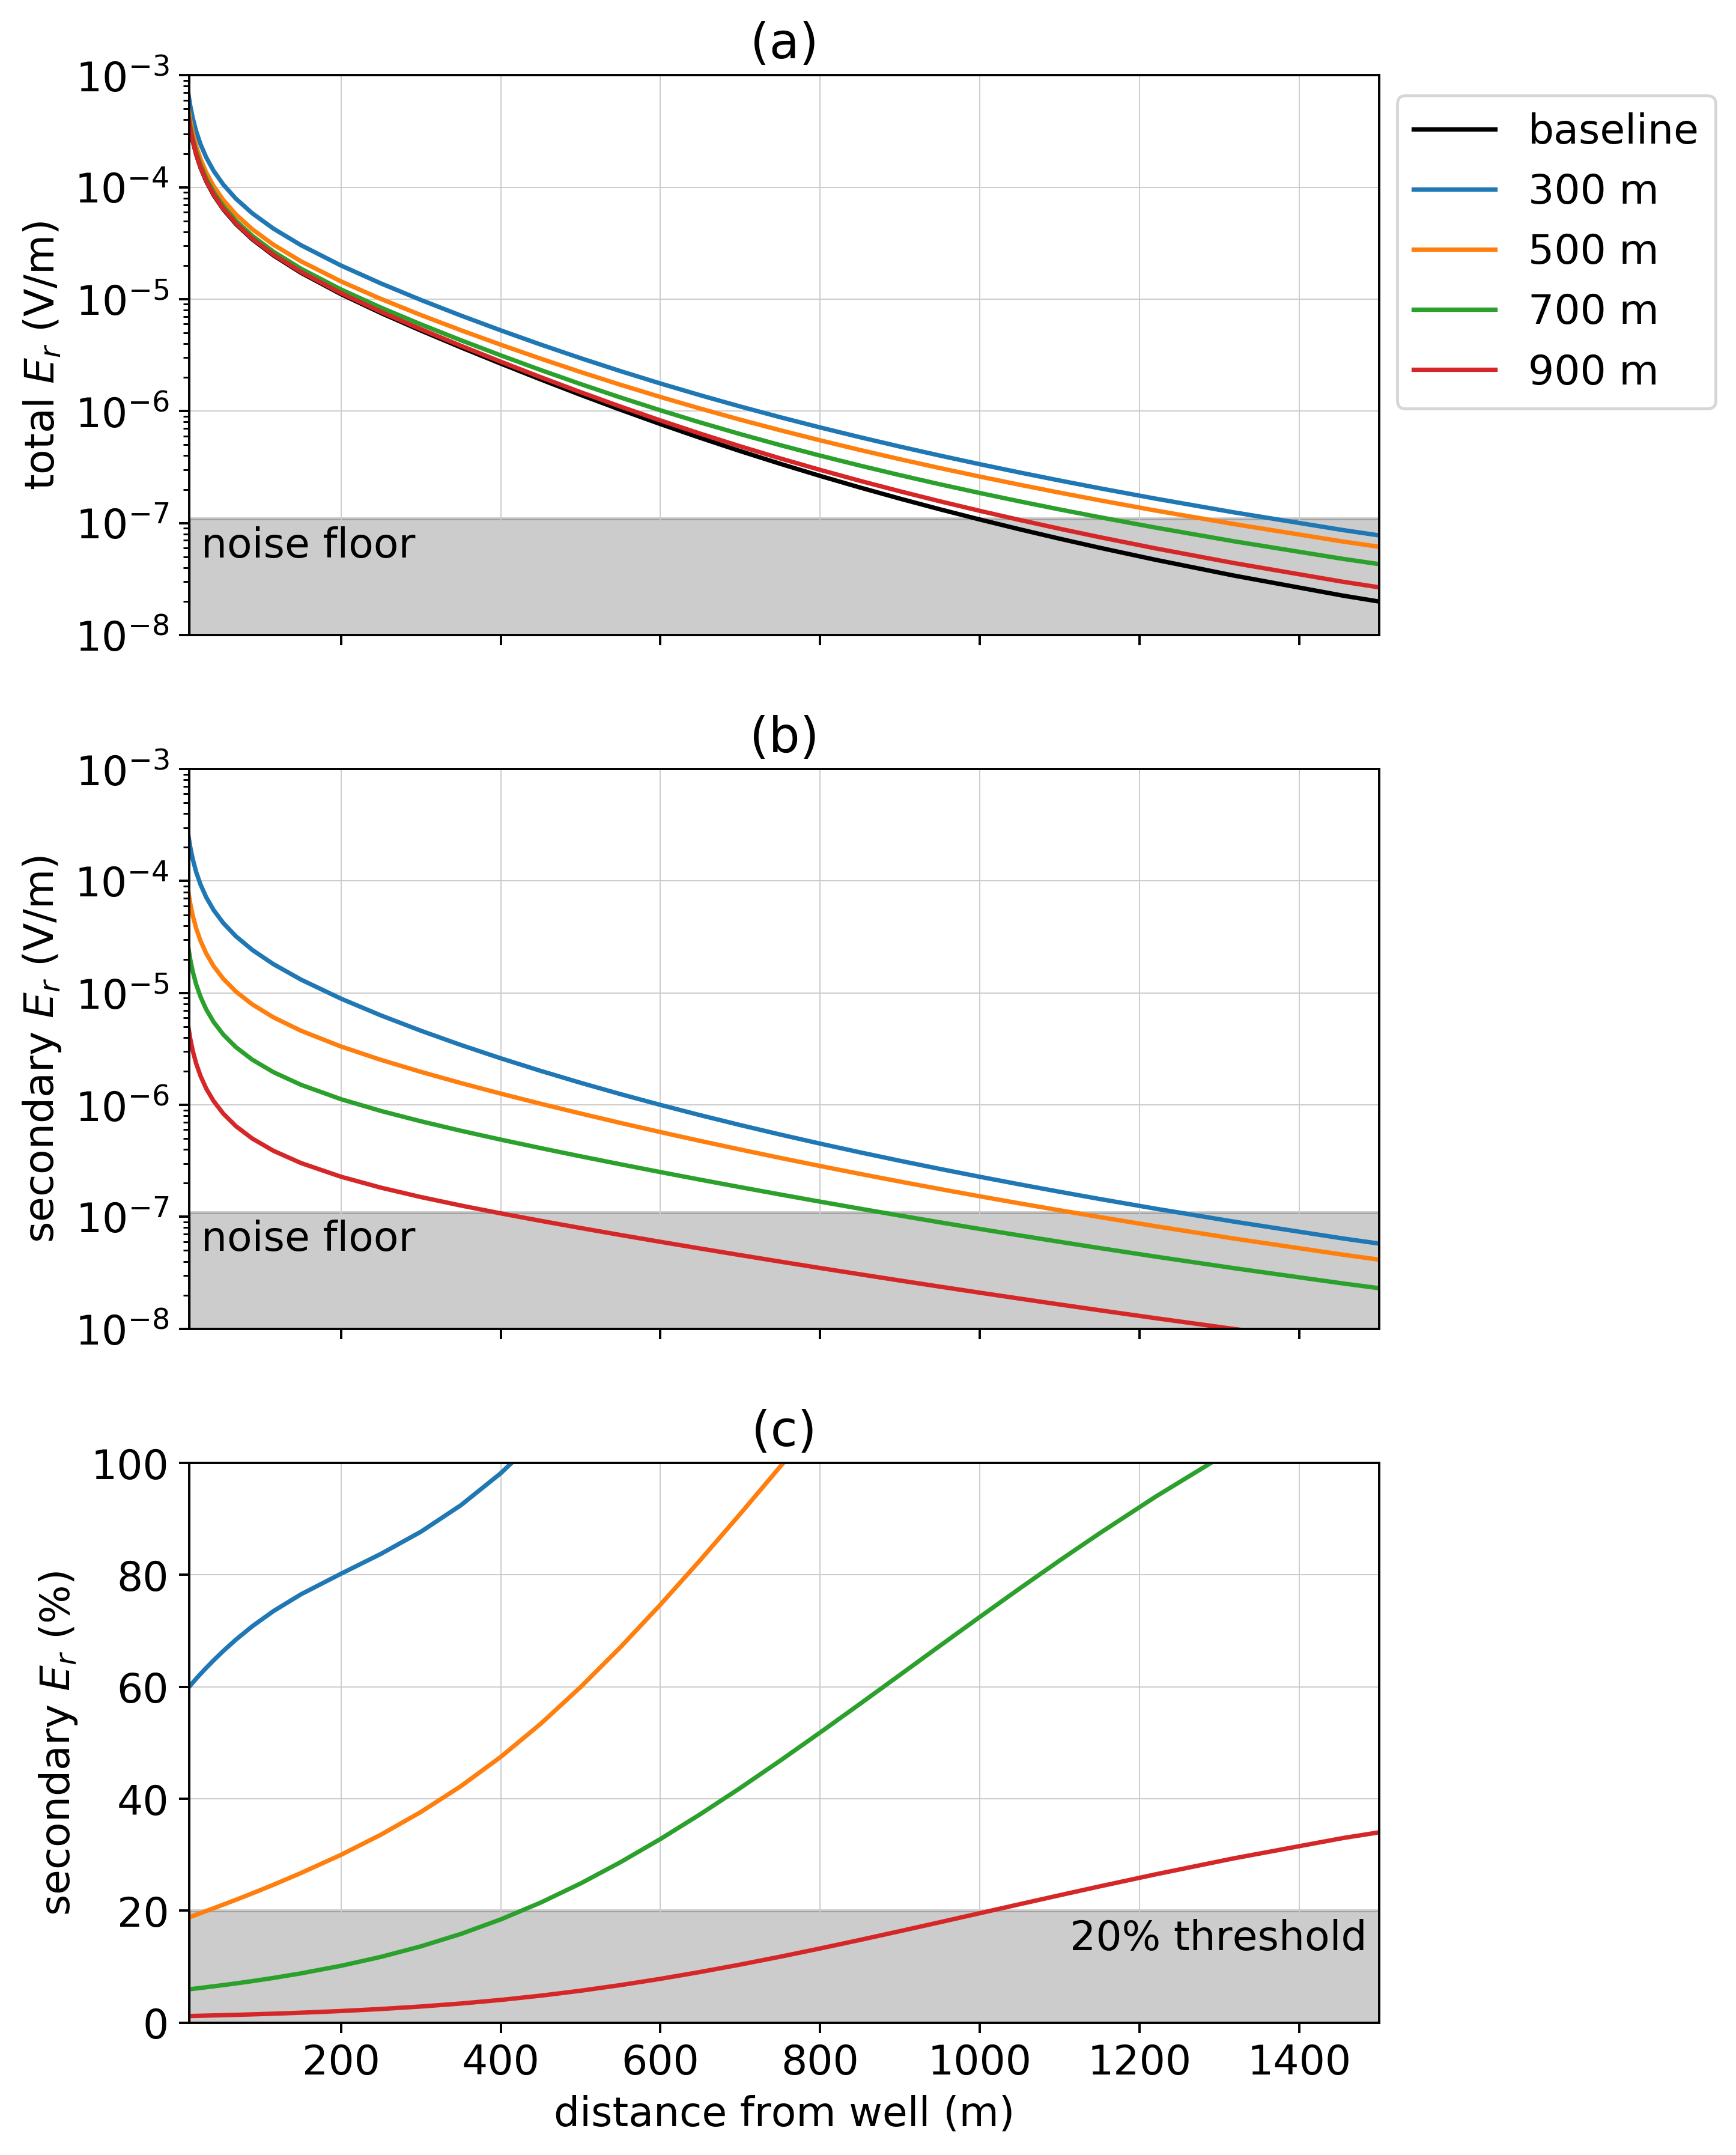
\includegraphics[width=0.8\textwidth]{figures/integrity_depth.png}
    \end{center}
\caption{
    Radial electric field as the depth of the flaw along a 1km long well is varied.
    The positive electrode is connected to the top of the casing, the negative electrode
    is positioned 500m away and data are measured along a line $90^\circ$ from the
    source electrodes. In (a), we show the total electric field for four flawed wells,
    each with a 10m flaw at the depth indicated on the legend. The black line shows
    the radial electric field due to an intact well; we define this as the primary.
    In (b), the secondary radial electric field is plotted and in (c), we show the
    secondary radial electric field as a percentage of the primary.
}
\label{fig:integrity_depth}
\end{figure}


\subsubsection{Background conductivity}

The total charge on the well is controlled by the contrast in conductivity between the steel-cased well and the surrounding geology. Increasing the conductivity of the background reduces that contrast thus reducing the amount of charge on the well. The result is a decrease in the total electric field at the surface. Similarly, the strength of the secondary dipolar charge introduced with the presence of an impairment also depends upon the available charge and will also be reduced with increasing background conductivity. In Figure \ref{fig:integrity_conductivity}, I have adopted the same model of a 1 km well with a 10 m impairment at 500 m depth, and show the radial electric field for the flawed (solid lines) and intact (dashed lines) well as the background conductivity is varied. A resistive background promotes the strongest total and secondary signals. As the conductivity increases, detectability becomes more challenging; at a conductivity of $3 \times 10^{-1}$ S/m, the flaw at 500 m depth is undetectable as there is no overlap in the regions where the secondary signal is above the noise floor and where it comprises a significant percentage of the primary.


\begin{figure}
    \begin{center}
    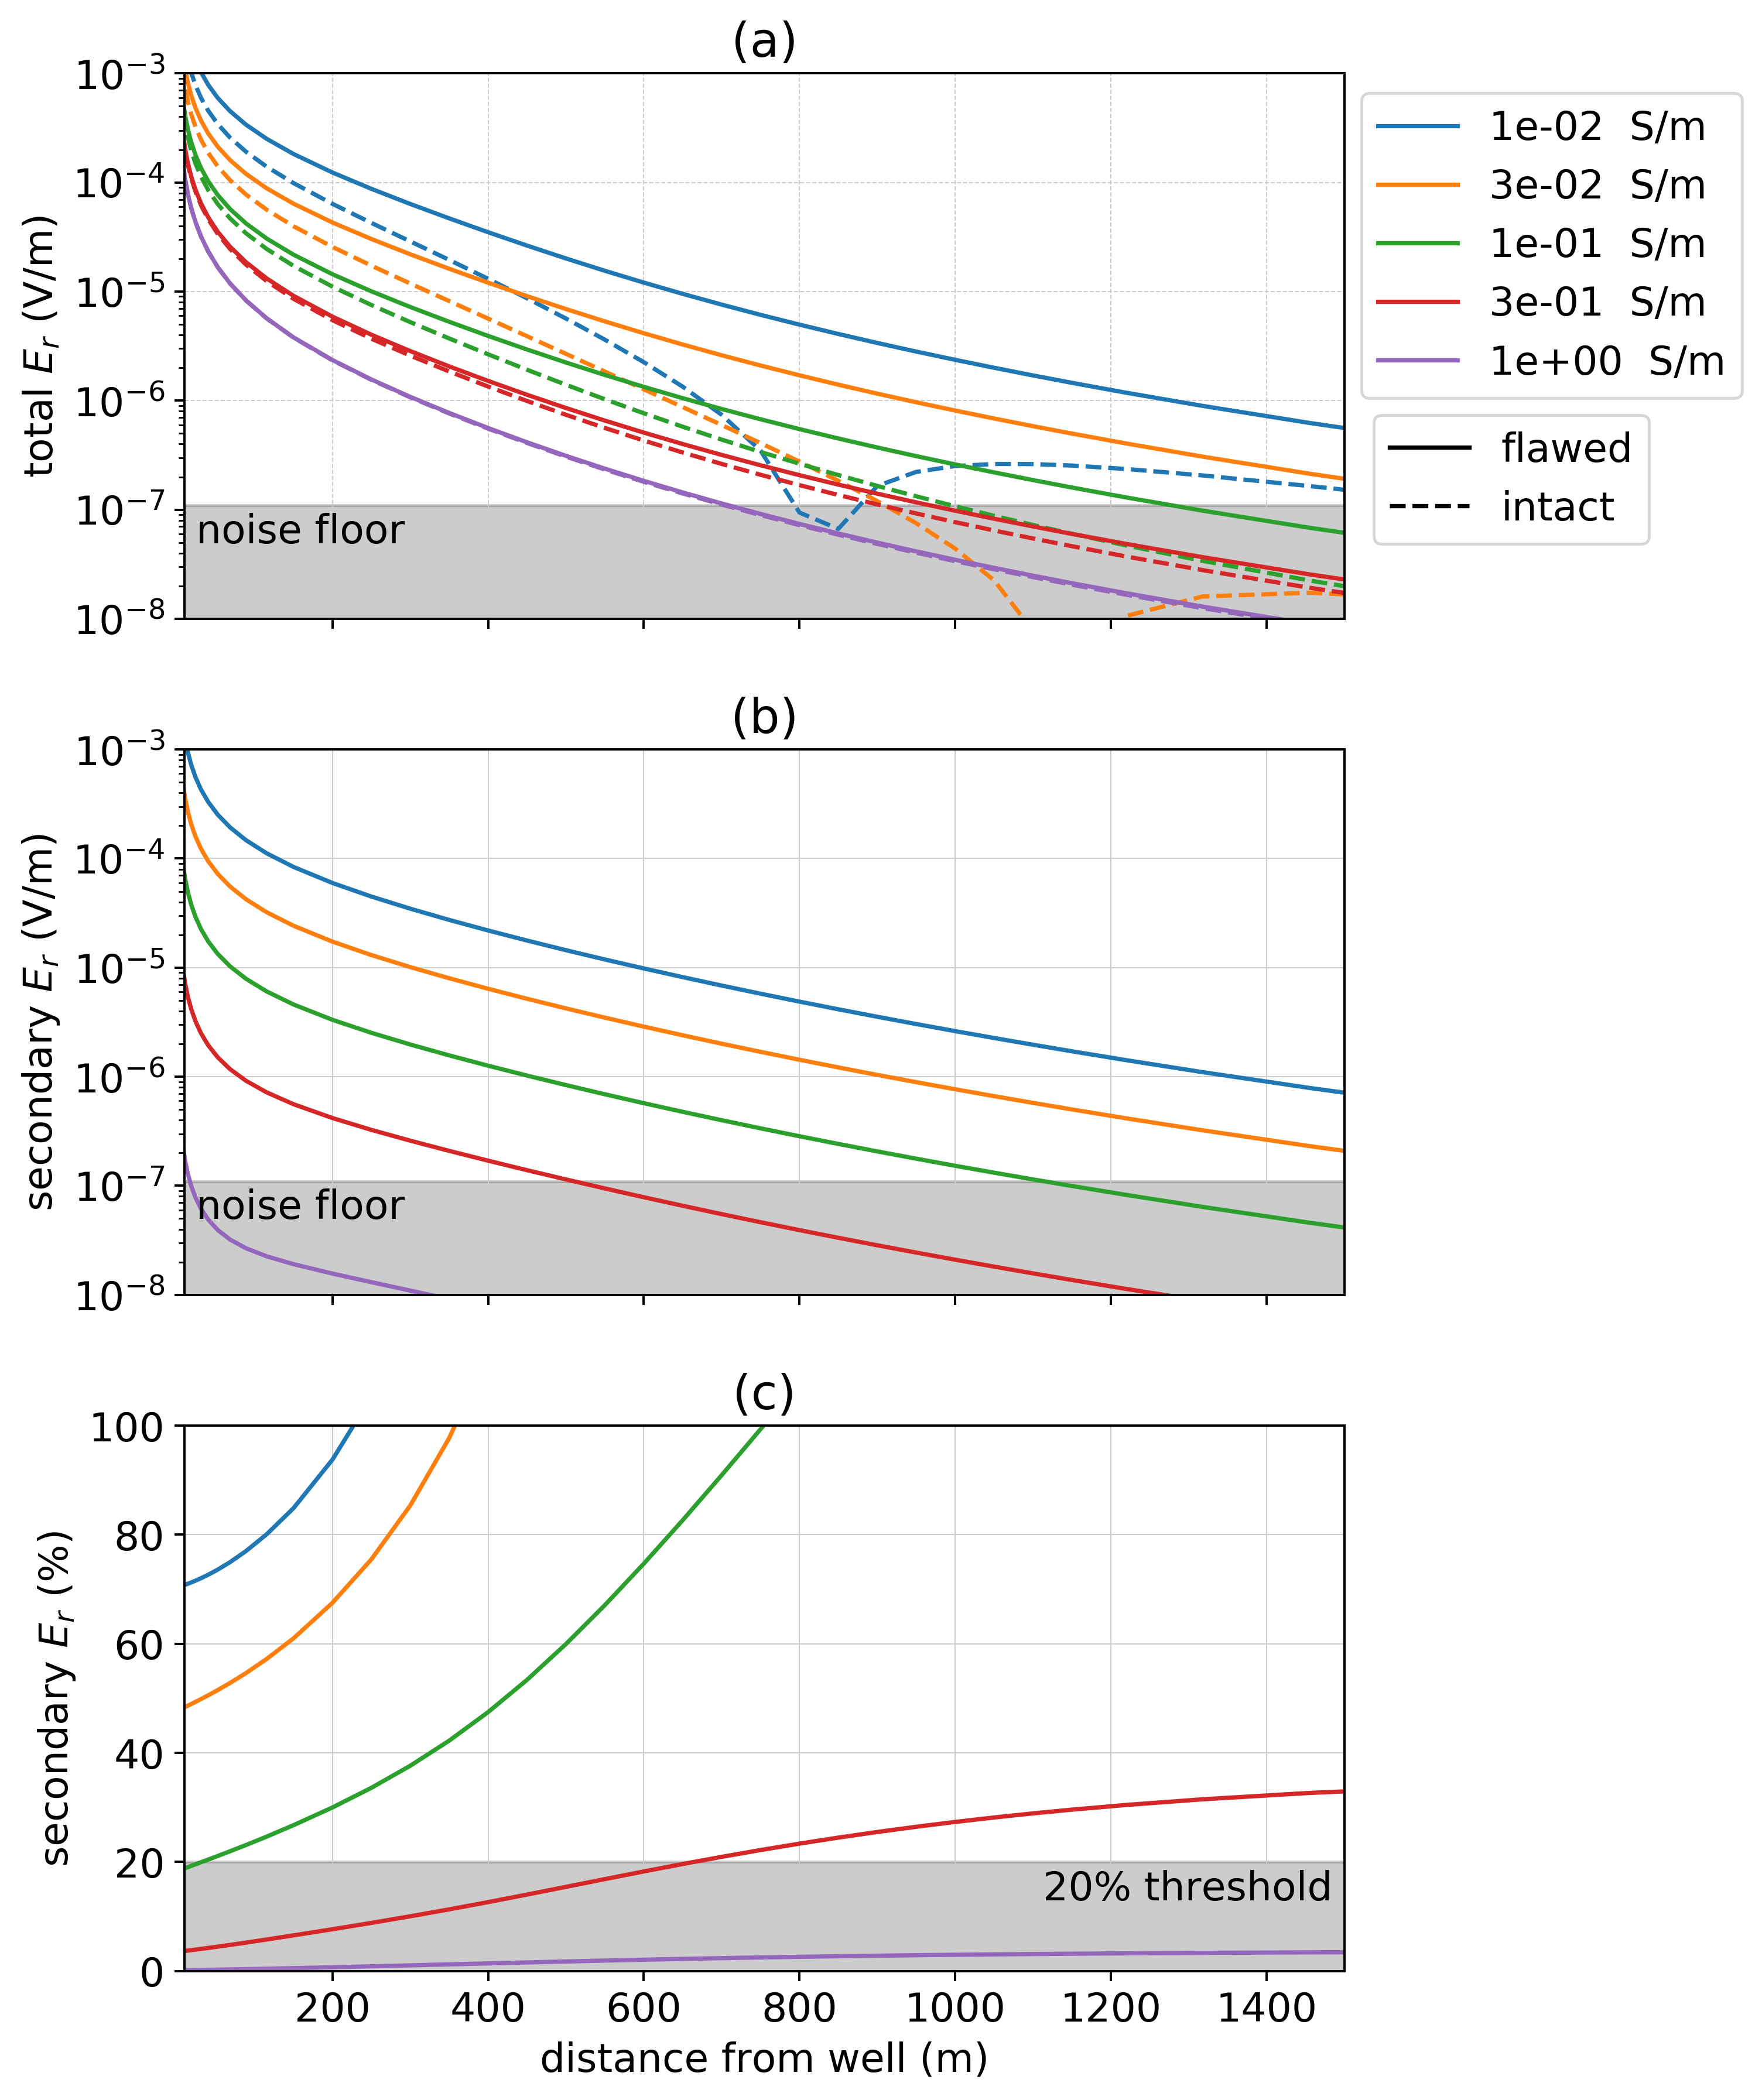
\includegraphics[width=0.8\textwidth]{figures/dc_casing/integrity_conductivity.png}
    \end{center}
\caption{
    Radial electric field as the conductivity of the background is varied for a 1km well with a 10m flaw at 500m depth.
    The positive electrode is connected to the top of the casing, the negative electrode
    is positioned 500m away and data are measured along a line $90^\circ$ from the
    source electrodes. In (a), we show the total electric field for five different background conductivities,
    each indicated on the legend. The solid lines indicate the response of the flawed well and the dashed lines indicate the response of the intact well (the primary).
    In (b), the secondary radial electric field is plotted and in (c), we show the
    secondary radial electric field as a percentage of the primary.
}
\label{fig:integrity_conductivity}
\end{figure}


Variations in the background geology will also influence the distribution of charges and thus the measured signal at the surface. To examine the challenges introduced when variable geology is considered, I will introduce a layer into the model and vary its conductivity. The layer is 50 m thick and its top is at 400 m depth. The flaw will again be positioned at 500 m depth, and the background conductivity is $10^{-1}$ S/m. The return electrode is 500 m from the well, and radial electric field data are measured along a line perpendicular to the source. In Figure \ref{fig:integrity_layer}, I show data for a flawed well (solid) and intact well (dashed) for scenarios in which a conductive or resistive layer is positioned above the flaw. The presence of a resistive layer improves detectability, while a conductive layer reduces detectability.

\begin{figure}
    \begin{center}
    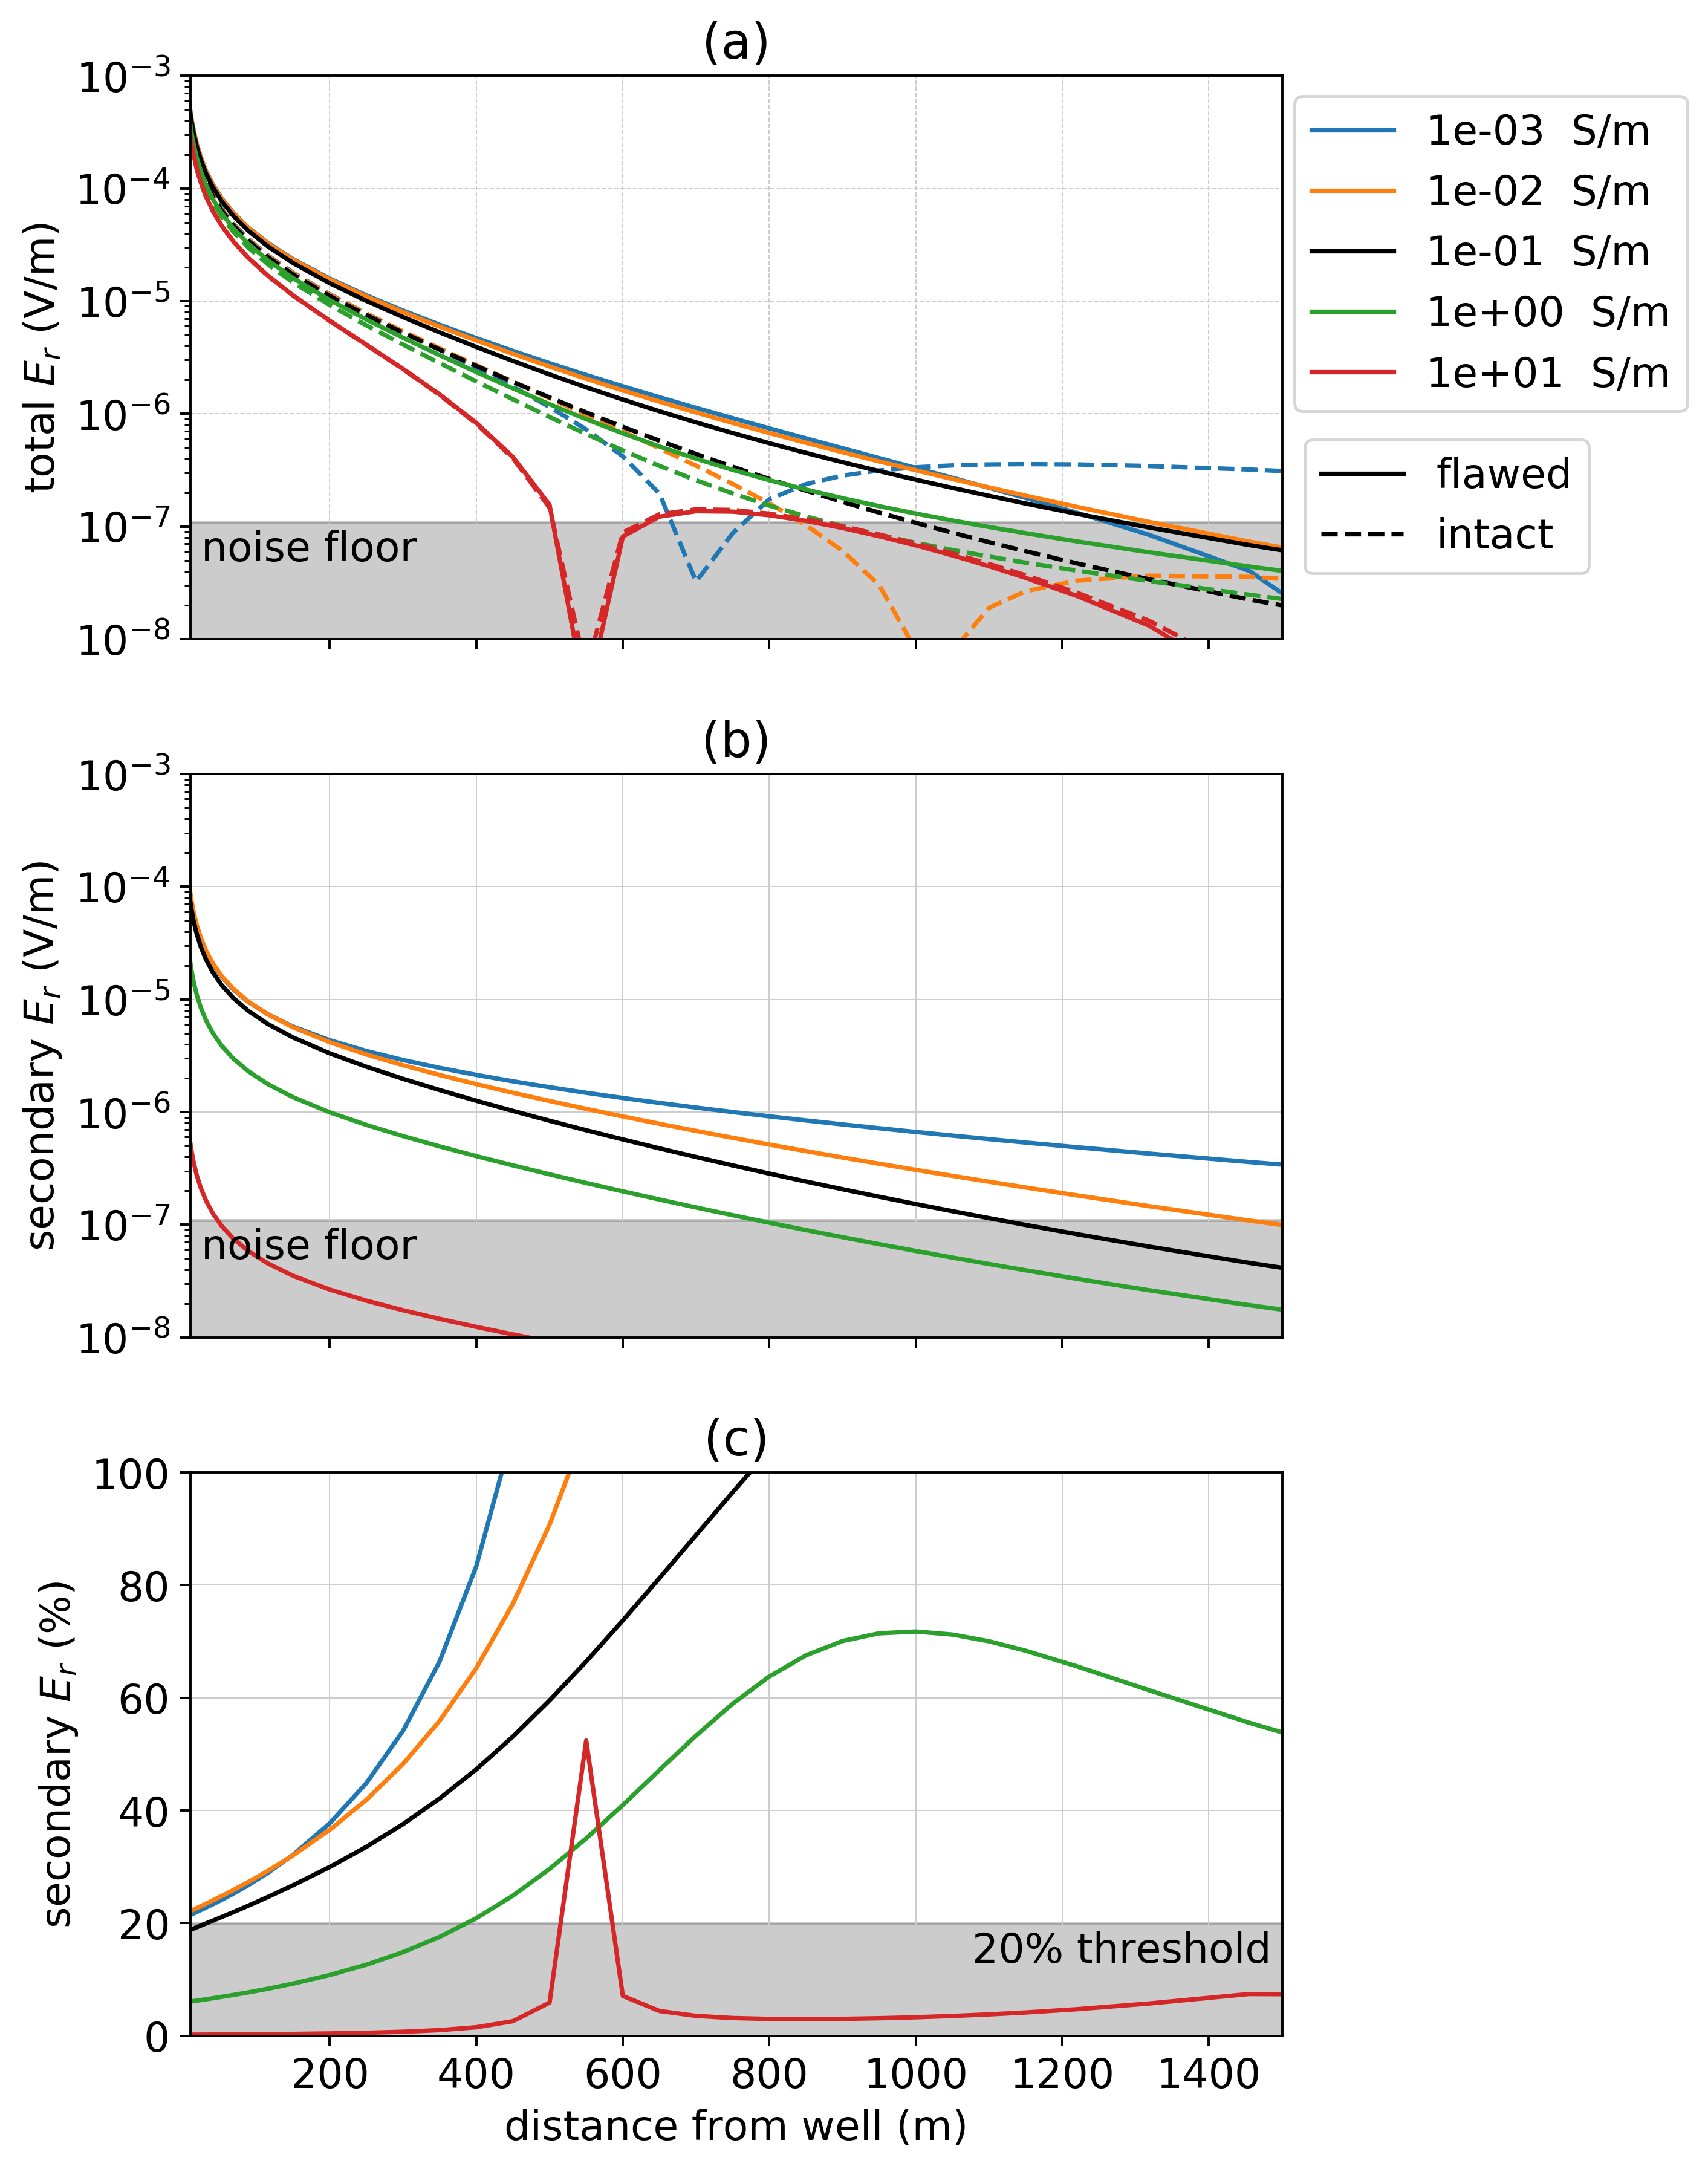
\includegraphics[width=0.8\textwidth]{figures/dc_casing/integrity_layer.png}
    \end{center}
\caption{
    Radial electric field as the conductivity of a 50 m thick layer positioned at 400 m depth is varied.
    The positive electrode is connected to the top of the casing, the negative electrode
    is positioned 500 m away and data are measured along a line $90^\circ$ from the
    source electrodes. In (a), we show the total electric field five different layer conductivities.
    The black line shows the scenario where the layer has the same conductivity as the background.
    The dashed-lines indicate the intact well and the solid lines indicate the flawed well.
    In (b), the secondary radial electric field is plotted (with respect to an intact well primary)
    and in (c), we show the
    secondary radial electric field as a percentage of the primary.
}
\label{fig:integrity_layer}
\end{figure}


To understand the physical phenomena governing this, I have plotted a cross section through: (a) the model, (b) the currents, (c) the charges, and (d) the electric field in Figure \ref{fig:integrity_layer_physics} for (first row) a model of an intact well with a conductive layer present, (second row) a flawed-well model including a conductive layer, (third row) a model of an intact well with a resistive layer, and (fourth row) a flawed-well model including the resistive layer. For the comparison, there is two orders of magnitude difference between the background and the layer. When a conductive layer is present, we see that it acts to ``short-circuit'' the system as there is significant current leak-off into that layer. This reduces the amount of current that reaches the flawed section of the well and decreases the total charge on the well, which is the source of our signal. Conversely, when a resistive layer is present, there is less leak-off of currents. In fact, \cite{Yang2016} showed that rather than leaking-off, currents can enter the casing if a resistive layer is present. In terms of detecting a flaw beneath a resistive layer, this means that the current density and charge along the well increases, thus amplifying the response due to the flaw.

\begin{figure}
    \begin{center}
    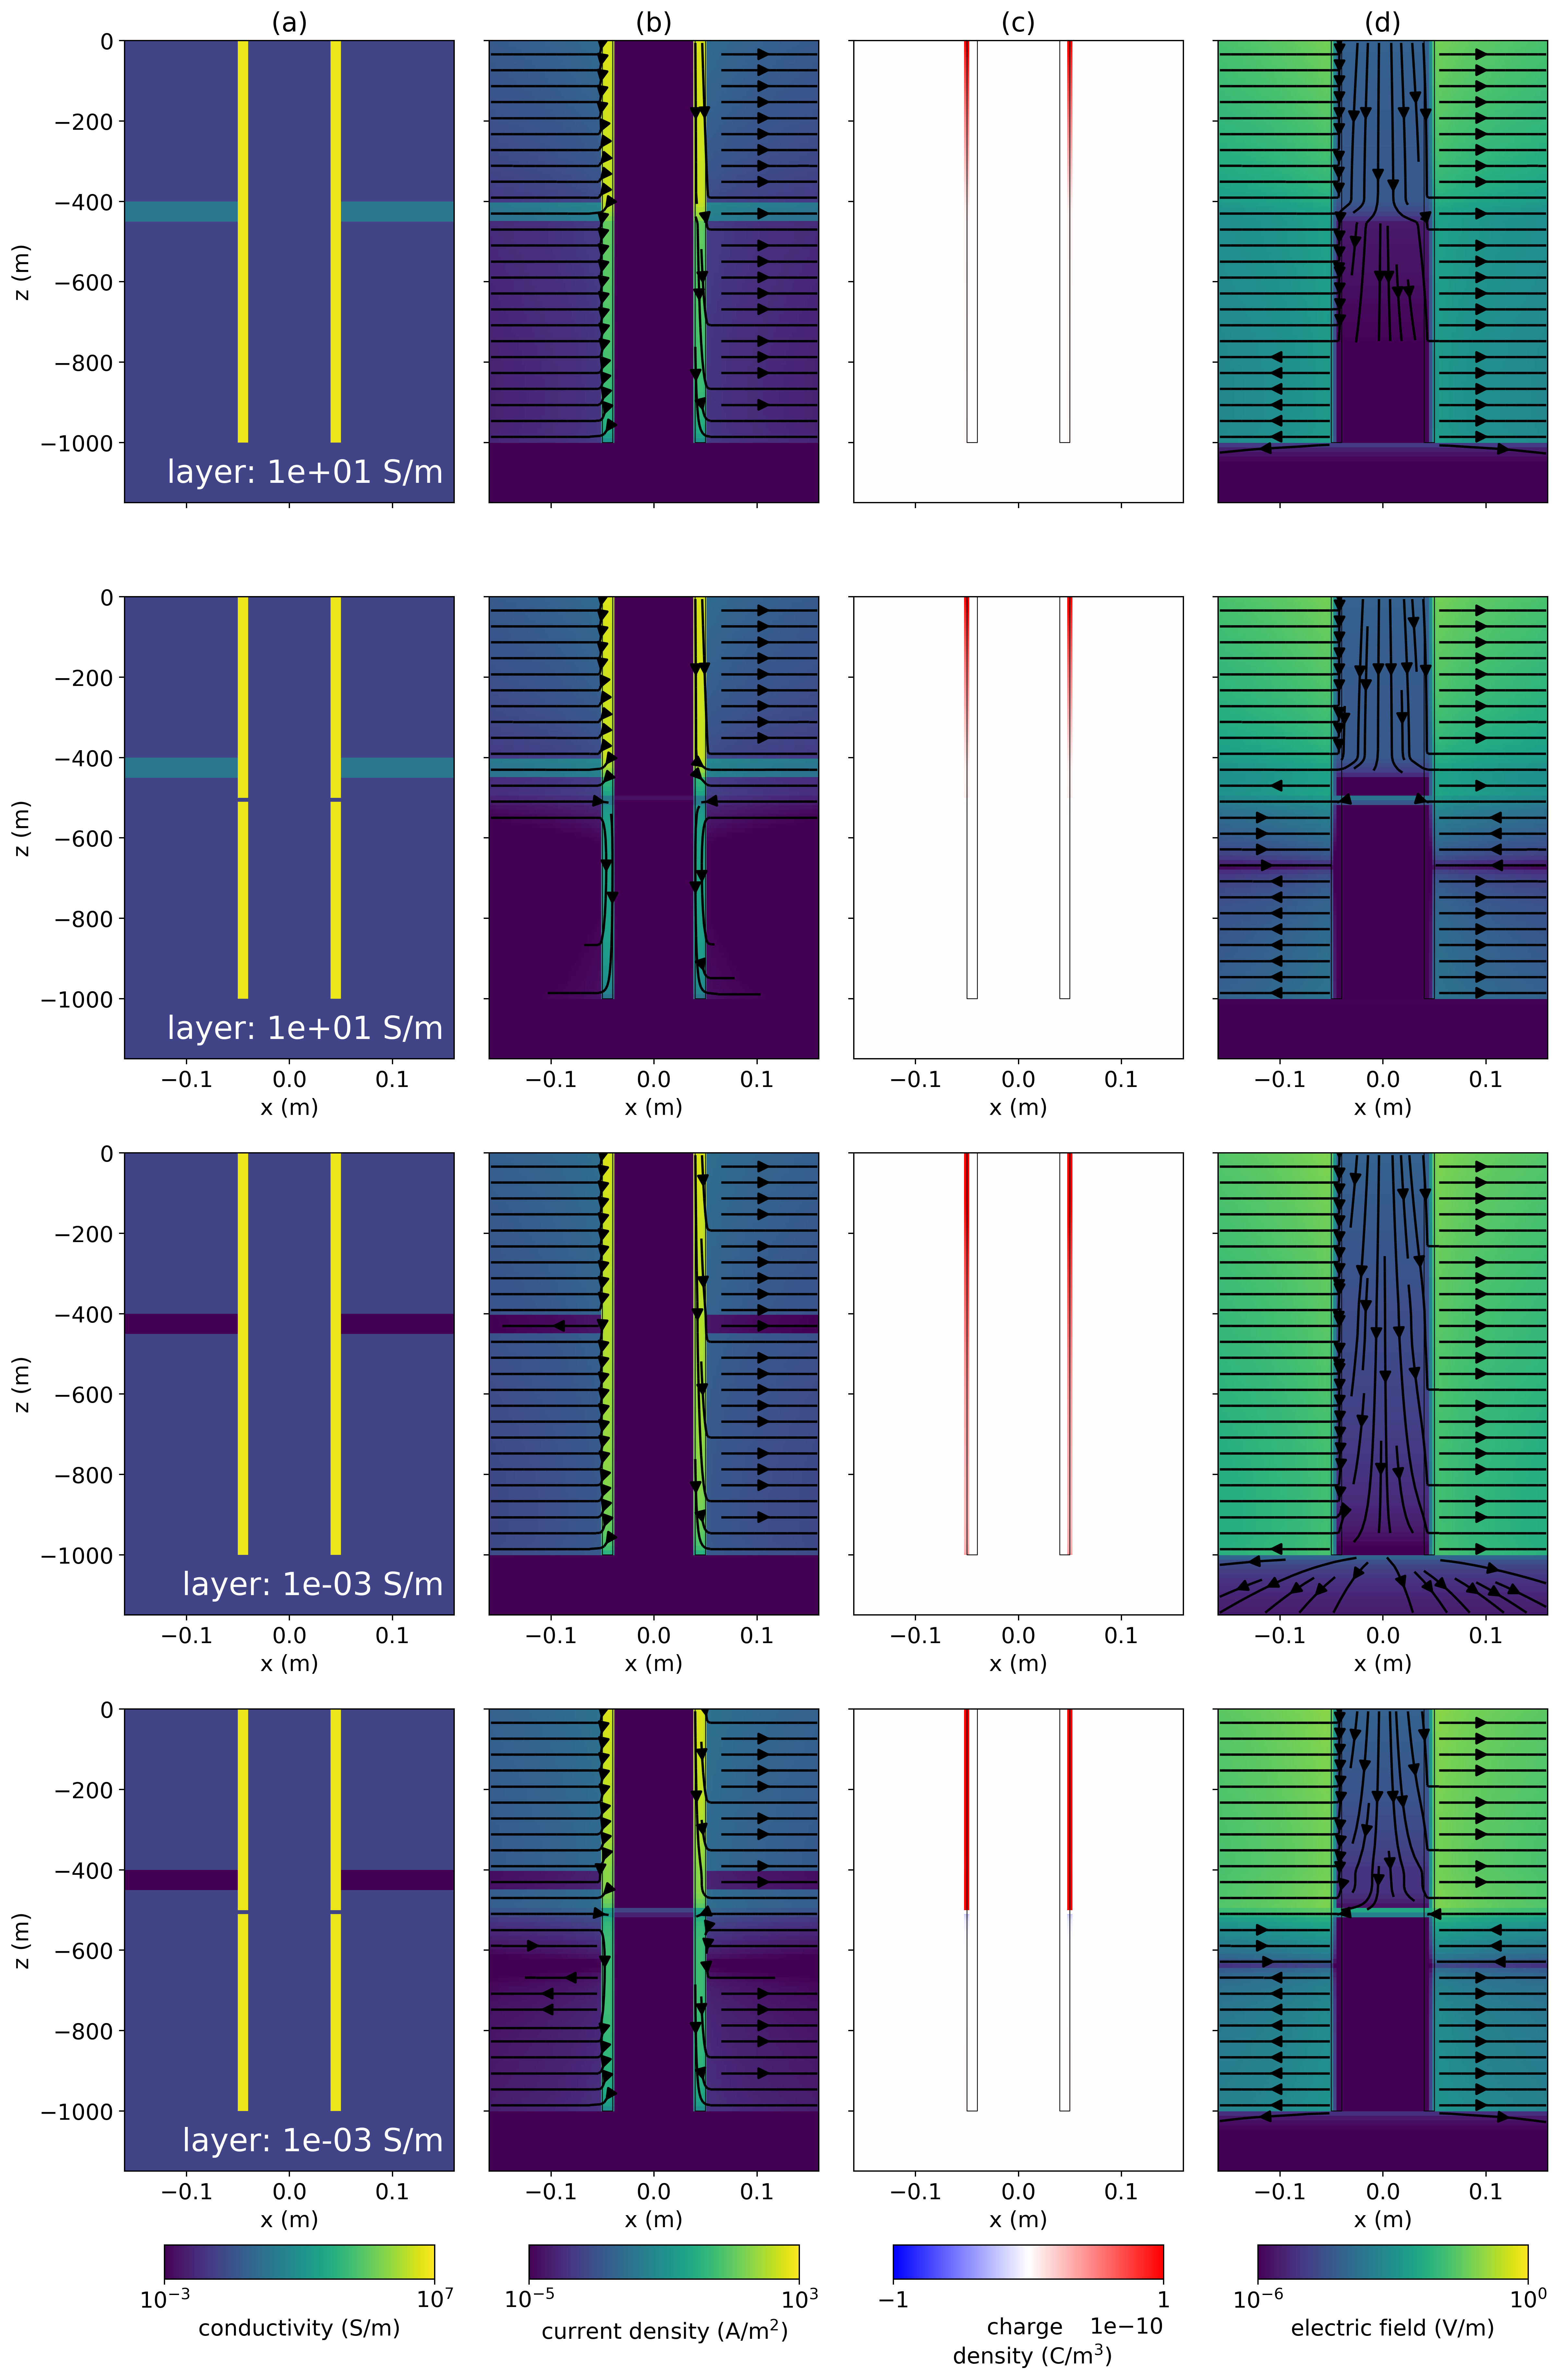
\includegraphics[width=0.8\textwidth]{figures/dc_casing/integrity_layer_physics.png}
    \end{center}
\caption{
    Cross section showing: (a) electrical conductivity, (b) current density, (c) charge density,
    and (d) electric field for a top-casing DC resistivity experiment over models with a conductive layer
    (top two rows) and a model with a resistive layer (bottom two rows). The layer extends from
    400 m to 450 m depth. The plots in the second and fourth rows correspond to models with a 10 m flaw at 500 m depth.
}
\label{fig:integrity_layer_physics}
\end{figure}


\subsubsection{Conductivity of the casing}
The conductivity of the casing is also relevant to how the charges are distributed along its length. For highly conductive wells, the charge along the length of the well is approximately uniform, for more resistive wells, the charges follow an exponential decay, as shown in Figure \ref{fig:casing_charge_sigma_casing}. \cite{Schenkel1991} described the decay of currents, and thus the distribution of charges along the length of a well, in terms of the conduction length,
\begin{equation}
     \delta_L = \sqrt{\frac{S_c}{\sigma_0}} = \sqrt{\frac{2\pi r t \sigma_c}{\sigma_0}}
\label{eq:conduction_length}
\end{equation}

Where $S_c$ is the cross-sectional conductance of the casing ($S_c = 2\pi r t \sigma_c$ for a casing with radius $r$, thickness $t$, conductivity $\sigma_c$ and has units of [S $\cdot$ m]) and $\sigma_0$ is the conductivity of the background. The conduction length is akin to skin depth in electromagnetics and is the depth at which  the amplitude of currents have decreased by a factor of $e^{-1}$. Casing conductivities of $5 \times 10^5$ S/m, $5 \times 10^6$ S/m, and $5 \times 10^7$ S/m correspond to conduction lengths of $\sim 180$ m, $560$ m, $1800$ m. For the most resistive well shown, $5 \times 10^{5}$ S/m, the vast majority of current has decayed well before it reaches the flaw; the majority of charges are concentrated where the currents leak off, near the top of the well. Correspondingly, there is greater sensitivity to a flaw in a conductive well than in a resistive well, as is reflected in the radial electric field data shown in Figure \ref{fig:integrity_conductivity_casing}.


\begin{figure}
    \begin{center}
    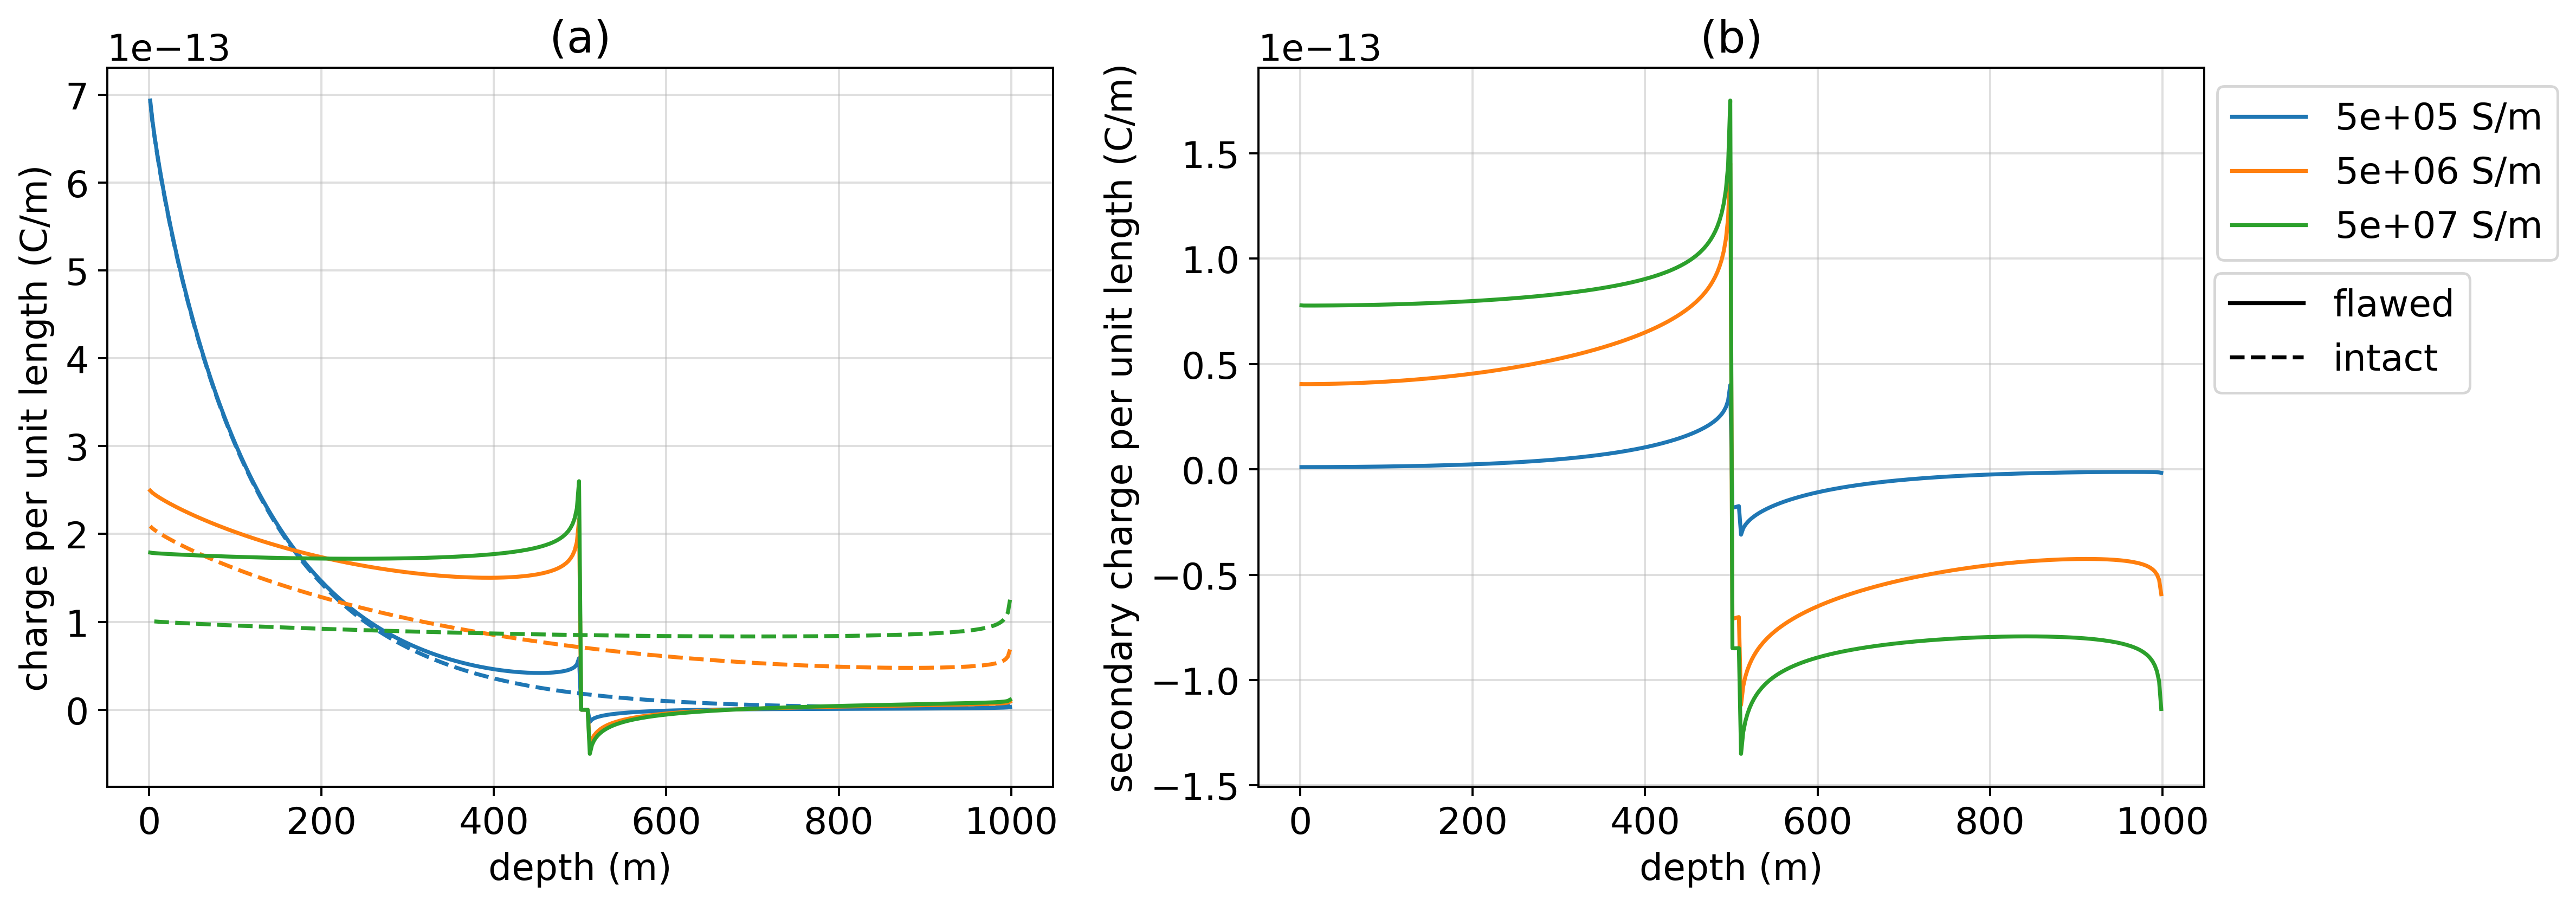
\includegraphics[width=\textwidth]{figures/dc_casing/casing_charge_sigma_casing.png}
    \end{center}
\caption{
    (a) Charge along the length of wells with three different
    conductivities (each indicated by a different color in the legend).
    The intact wells are denoted with dashed lines and the flawed wells
    are denoted with solid lines.
    (b) Secondary charge along the flawed and short wells. The primary is
    defined as the electric field due to the 1000m long intact well. The return electrode
    is 2000m away from the well.
}
\label{fig:casing_charge_sigma_casing}
\end{figure}




\begin{figure}
    \begin{center}
    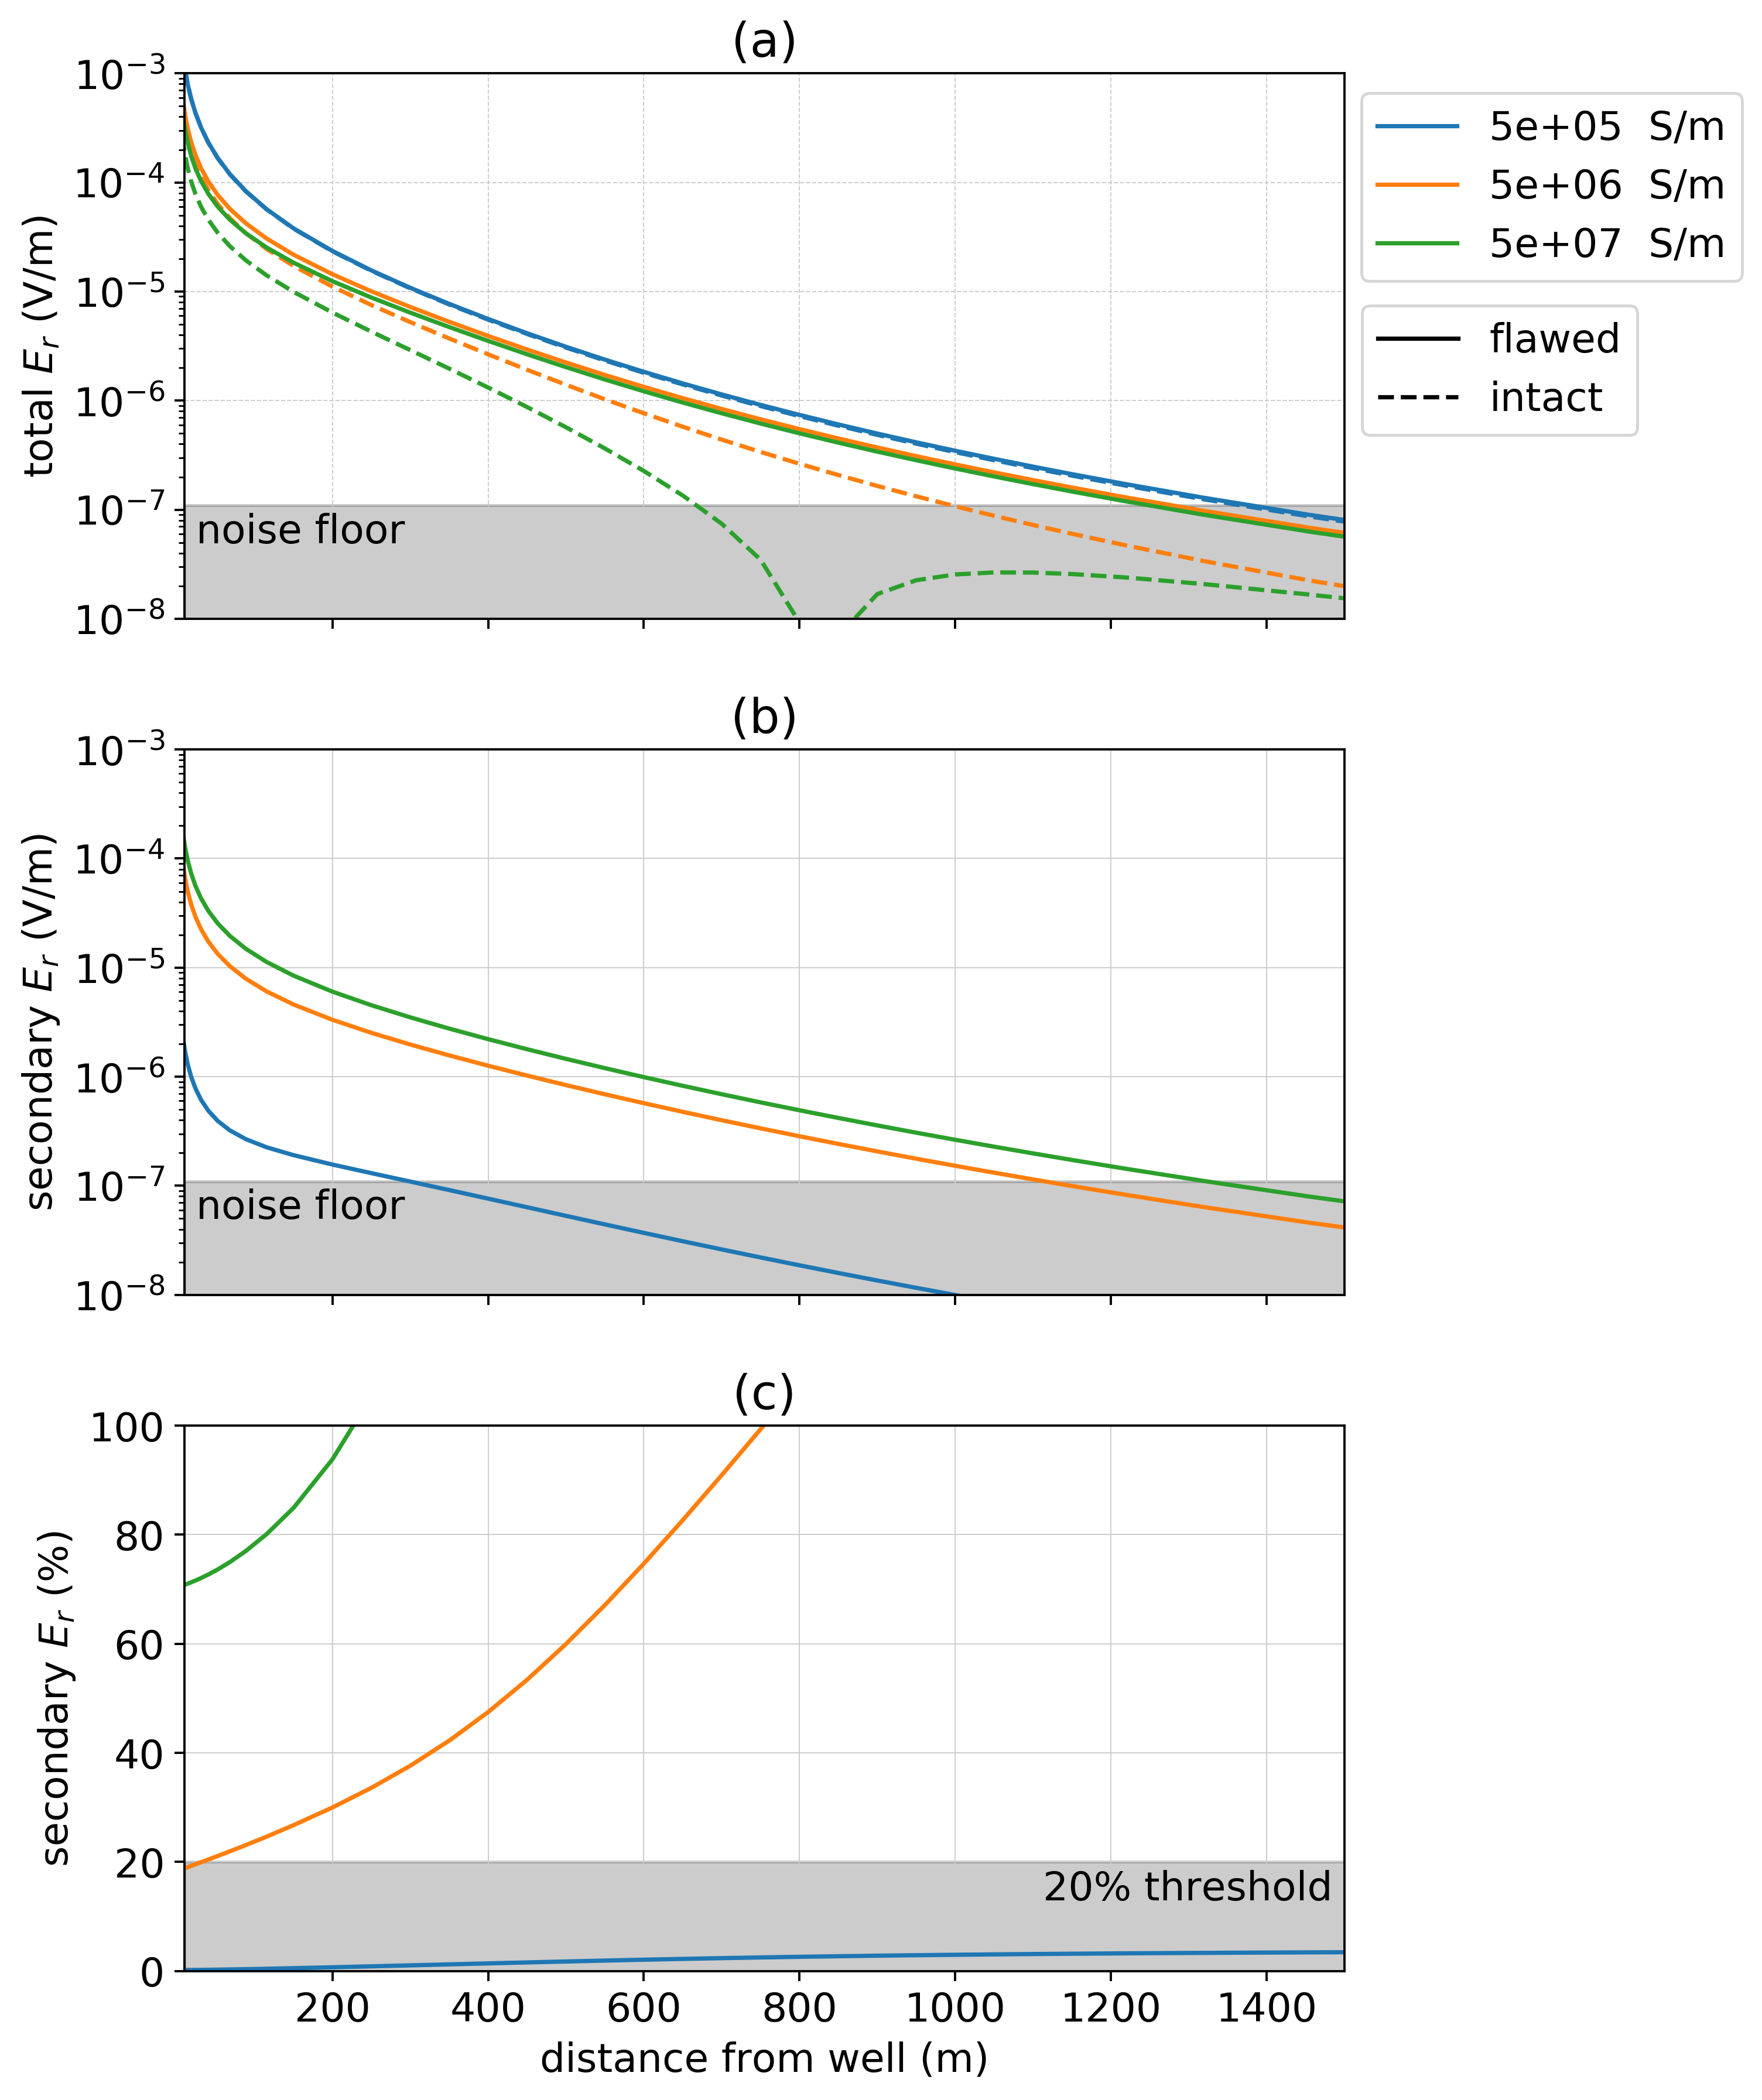
\includegraphics[width=0.8\textwidth]{figures/integrity_conductivity_casing.png}
    \end{center}
\caption{
    Radial electric field as the conductivity of the casing is varied for a 1km well with a 10m flaw at 500m depth.
    The positive electrode is connected to the top of the casing, the negative electrode
    is positioned 500m away and data are measured along a line $90^\circ$ from the
    source electrodes. In (a), we show the total electric field for three different casing conductivities,
    each indicated on the legend. The solid lines indicate the response of the flawed well and the dashed lines indicate the response of the intact well (the primary).
    In (b), the secondary radial electric field is plotted and in (c), we show the
    secondary radial electric field as a percentage of the primary.
}
\label{fig:integrity_conductivity_casing}
\end{figure}


\subsubsection{Partial flaw}
The above examples considered an impairment that affects the entire circumference of the casing. This may be suitable in some scenarios where a particular geologic unit subjects the well to corrosive conditions, however, flaws may also be vertical cracks along the well (e.g. if pipe burst occurs). This is a much more challenging problem for DC resistivity because, if only a portion of the circumference is impaired, there is still a high-conductivity pathway for currents to flow along the entire length of the well. To examine the feasibility of detecting a partial flaw, I have run simulations where half of the circumference of the casing is compromised, leaving the other-half intact.

I consider four different depth extents of the flaw between 10 m and 300 m; in all scenarios the top of the flaw is at 500 m. In Figure \ref{fig:integrity_partial_flaw}a, I have plotted the total radial electric field resulting from an intact well (black), wells where the entire circumference is compromised (solid) and wells in which 50\% of the circumference has been compromised (dashed); (b) and (c) show the secondary radial electric field and the secondary as a percentage of the primary, respectively. We see that the depth-extent of the flaw has little impact on the fully-compromised wells, which is consistent with the observations in our previous examples. However, if the well is partially flawed, we do see variation in the secondary response. By compromising 50\% of the circumference of the well, we have reduced the effective cross-sectional conductance over that portion of the well. Numerical experiments show that if, instead of introducing a flaw which comprises 50\% of the circumference of the well, we reduce the conductivity of the intact well by 50\% over the same depth extent as the flaw, we obtain similar, but not identical, responses at the surface. Although for extensive flaws, there is a small region over which the secondary signal is above the noise floor, there are no regions where this coincides with measurements where the secondary fields are a significant percentage of the primary. There may be a subset of circumstances, such as if the flaw is near to the surface, or if the background geology is sufficiently well-known so that the percent threshold can be reduced, where a partial flaw may be diagnosed, however, these results demonstrate that a partial flaw is a challenging target for a DC resistivity survey.


\begin{figure}
    \begin{center}
    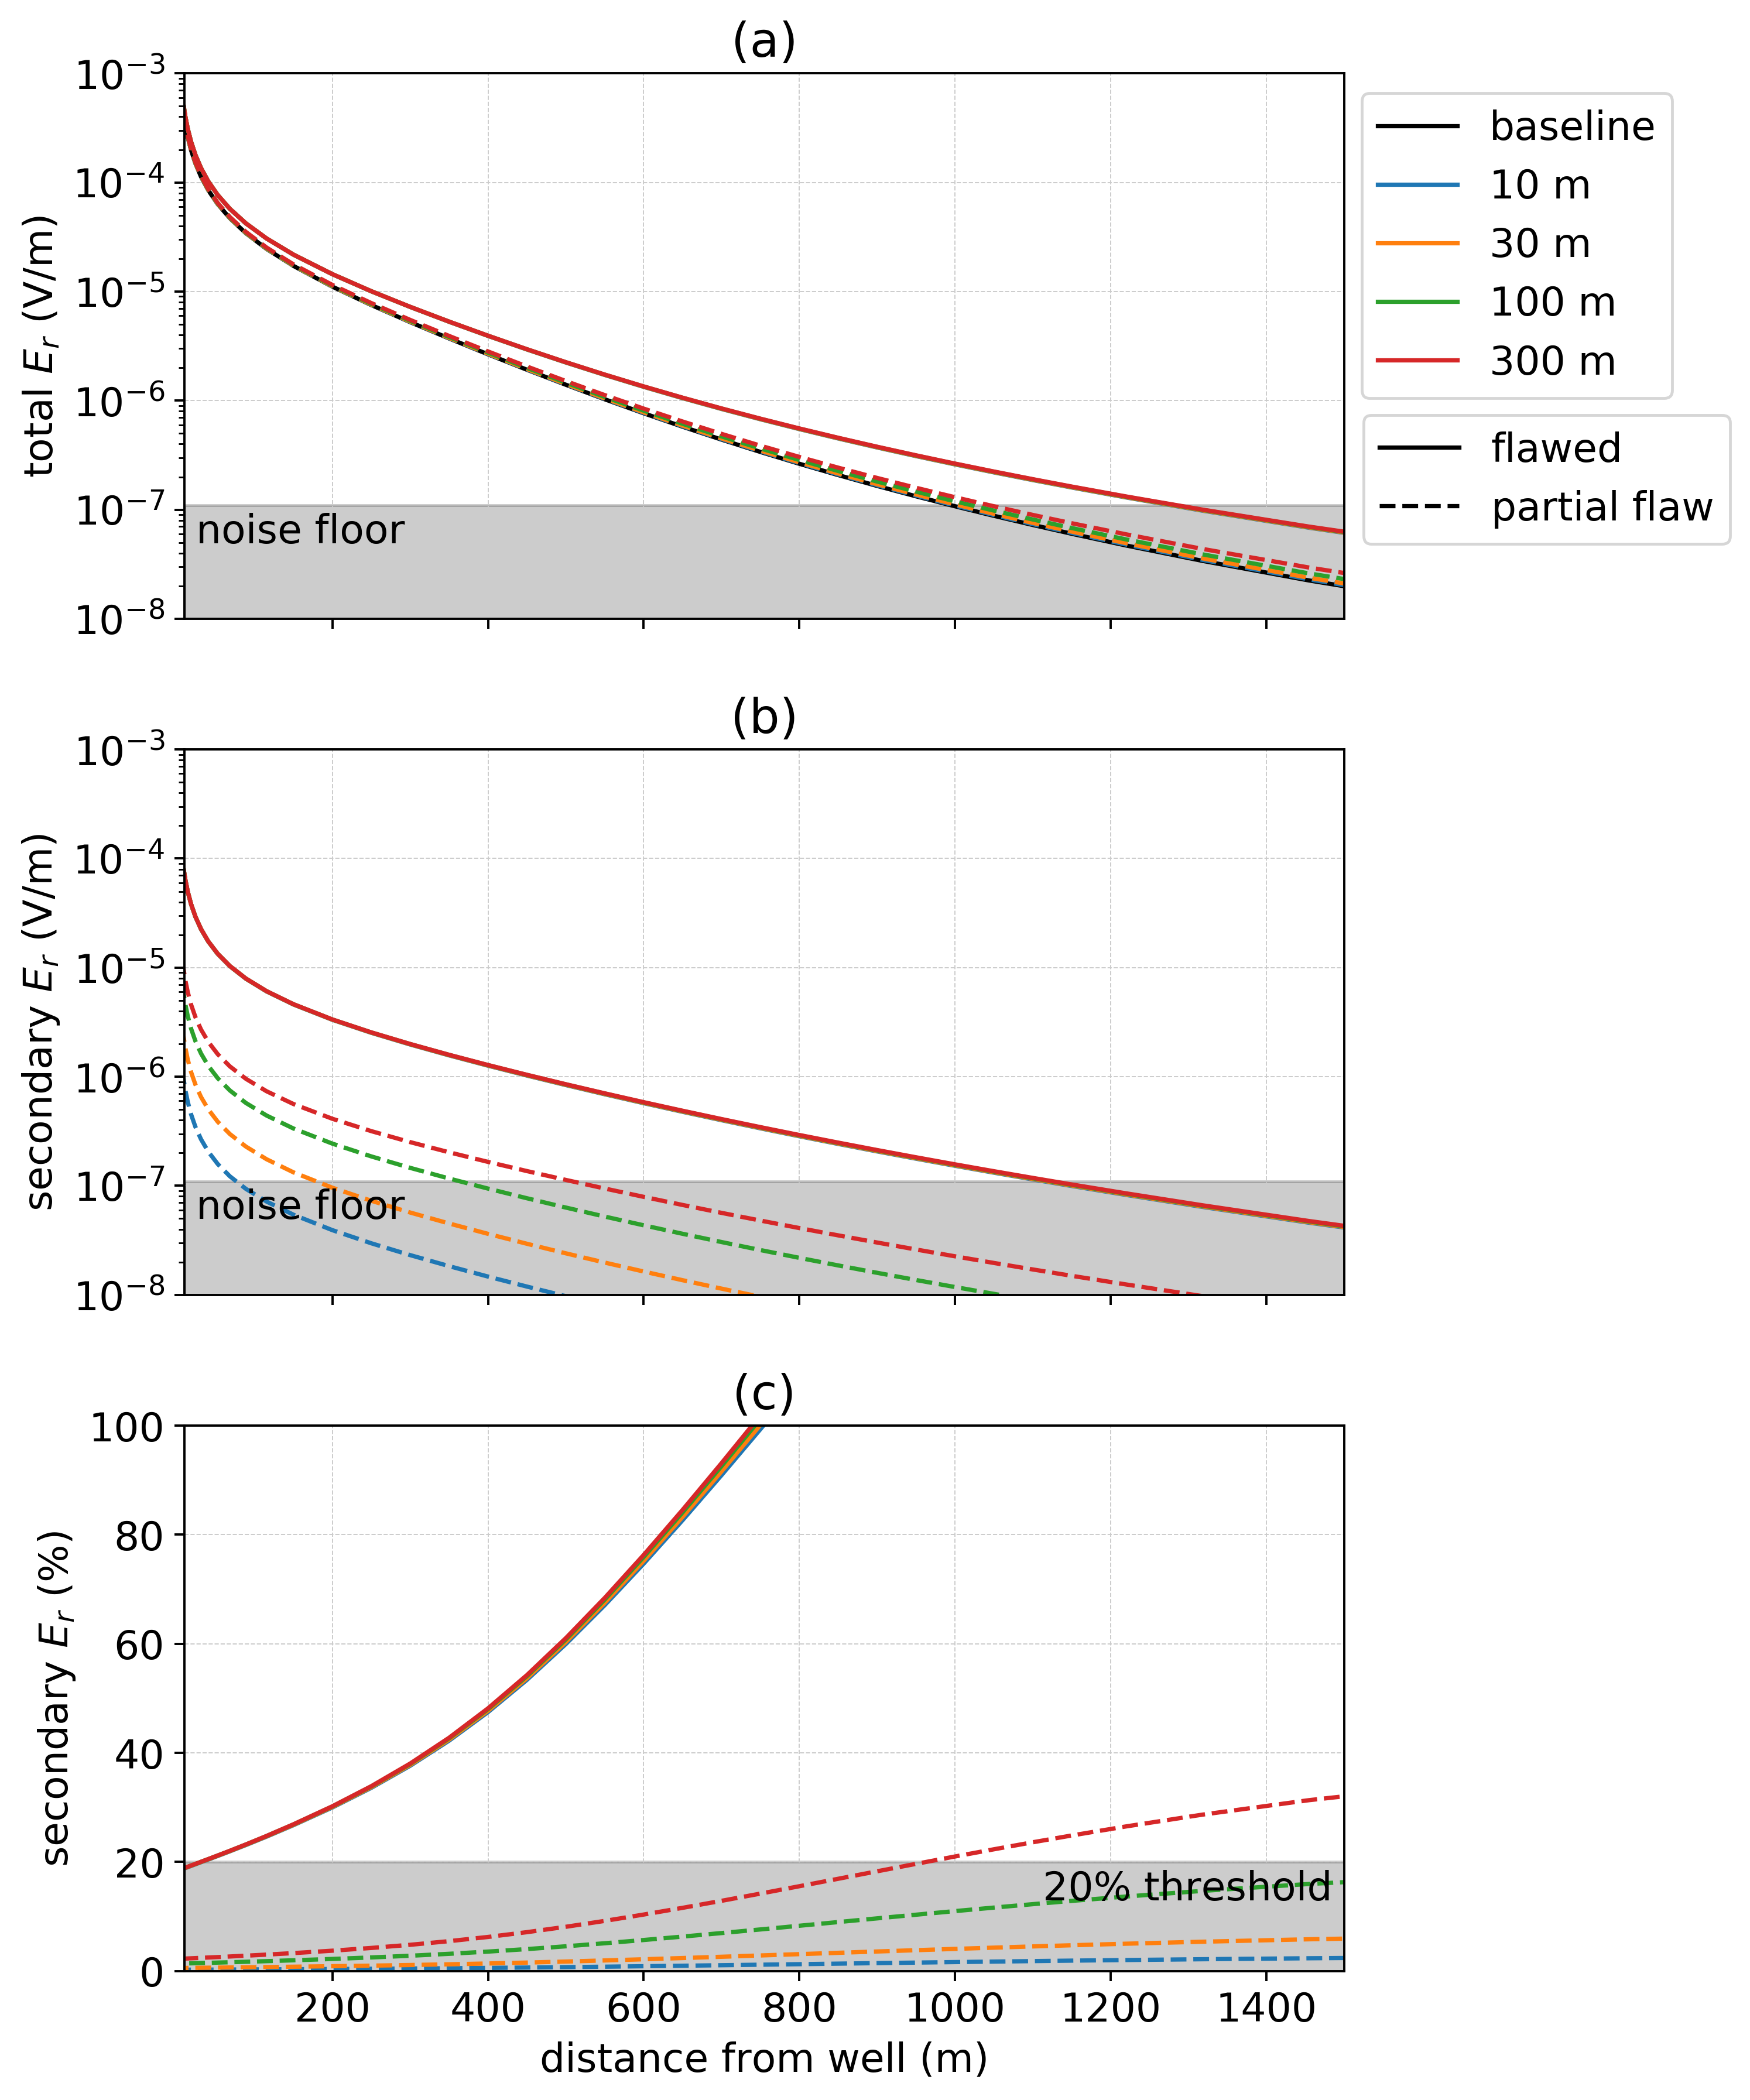
\includegraphics[width=0.8\textwidth]{figures/dc_casing/integrity_partial_flaw.png}
    \end{center}
\caption{
    Radial electric field as the vertical extent of the flaw is varied.
    The positive electrode is connected to the top of the casing, the negative electrode
    is positioned 500m away and data are measured along a line $90^\circ$ from the
    source electrodes. In (a), we show the total electric field four different flaw extents.
    The black line shows the response of the intact well.
    The dashed-lines indicate the partially flawed wells (50\% of the circumference is compromised)
    and the solid lines flawed wells in which the entire circumference of the well has been compromised.
    In (b), the secondary radial electric field is plotted (with respect to an intact well primary)
    and in (c), we show the secondary radial electric field as a percentage of the primary.
}
\label{fig:integrity_partial_flaw}
\end{figure}


\subsection{Summary}
In summary, I provided an overview of the fundamental physics governing the behavior of currents, charges, and electric fields in a top-casing DC resistivity experiment to detect an impairment in the well. If a flaw comprises the entire circumference of some depth interval along the casing, then the charges are concentrated in the portion of the well above the flaw, and to first approximation, the charge distribution is equal to that of a well which has been truncated at the depth of the flaw. This excess charge is the source of our signal. As it is cylindrically symmetric, the resultant secondary electric fields due to the flaw are purely radial. In terms of survey-design, we can take advantage of this knowledge and use the return electrode location to reduce coupling with the primary electric field in our data (as shown in Figure \ref{fig:integrity_e_fields}). Our ability to detect a flaw across the entire circumference of the casing depends upon the conductivity of the background and casing, as well as the depth of the flaw. Larger contrasts between the casing and the background (e.g. a more resistive background and / or a more conductive casing) increase the secondary response, as does decreasing the depth of the flaw. If only a portion of the circumference is impaired, leaving a conductive pathway connecting the top and bottom portions of the casing, the secondary signal is small and thus will be challenging to detect under most circumstances.

For the subset of scenarios where we do have data sensitivity to the flaw, an inverse problem can be solved to  estimate the depth of the impairment. One approach would be to use a reduced modeling procedure whereby only a few parameters are sought. For the case presented here, we might invert for a smooth background, the length of the well, and potentially the conductivity of the casing, if it is not known a-priori.

In the next section, I transition from viewing the casing as the target to working on the scale of a geophysical imaging application in reservoir monitoring and viewing the casing as a high-conductivity feature present in that setting.

\section{Survey design for exciting targets at depth}
\label{sec:survey_design}

There are many problems in hydraulic fracturing, carbon capture and storage and enhanced oil recovery that require targets to be illuminated and data to be acquired and inverted. Typically these experiments include steel-cased wells and the target of interest could be resistive or conductive. The target could be immediately adjacent to a well or offset from it, and the survey may employ electrodes on the surface or positioned down-hole. Similarly, receivers may be positioned on the surface or in adjacent boreholes. Each of these factors influences our ability to detect a target in our data.

Detectability of a target requires two steps: (1) source fields must excite the target, and (2) receivers must be positioned so that the secondary response is measurable. In this section, I focus on the first point -- exciting the target. I will examine the impact of source electrode locations, the physical properties of the target and the geometry of the target on our ability to excite a response.
\subsection{Source location}
I begin by examining the impact of the source electrode location on our ability to deliver current to a region of interest in the model. The model I consider is 1 km long well in a $10^{-1}$ S/m background. The well has a conductivity of $5 \times 10^6$ S/m, an outer diameter of 10 cm thickness, and a 1 cm thickness; these are the same parameters used for the casing integrity experiment described in the previous section. The conductivity of the fluid filling the casing is identical to that of the background. I am interested in effects near the well and thus the modeling can be carried out using the 2D cylindrical mesh provided that the return electrode is sufficiently far away. The return electrode is physically a disc of current at a radius equal to the distance of the return electrode from the well, in this case 2 km. The assumption of cylindrical symmetry and the use of a distant return electrode has similarly been applied in \cite{Schenkel1991}.

To examine the impact that the source electrode location has on our ability to excite a target, I consider the electrode locations shown in Figure \ref{fig:electrode_location}. Three of the electrodes are connected to the casing (tophole - blue, centered - green, and downhole - red); the remaining electrodes are not connected to the casing; these include the surface electrode (orange) as well as the five electrodes near the end of the pipe (purple - within the pipe, brown, pink, grey and yellow are beneath the end of the pipe). The surface electrode is offset from the well by 0.1 m.



\begin{figure}
    \begin{center}
    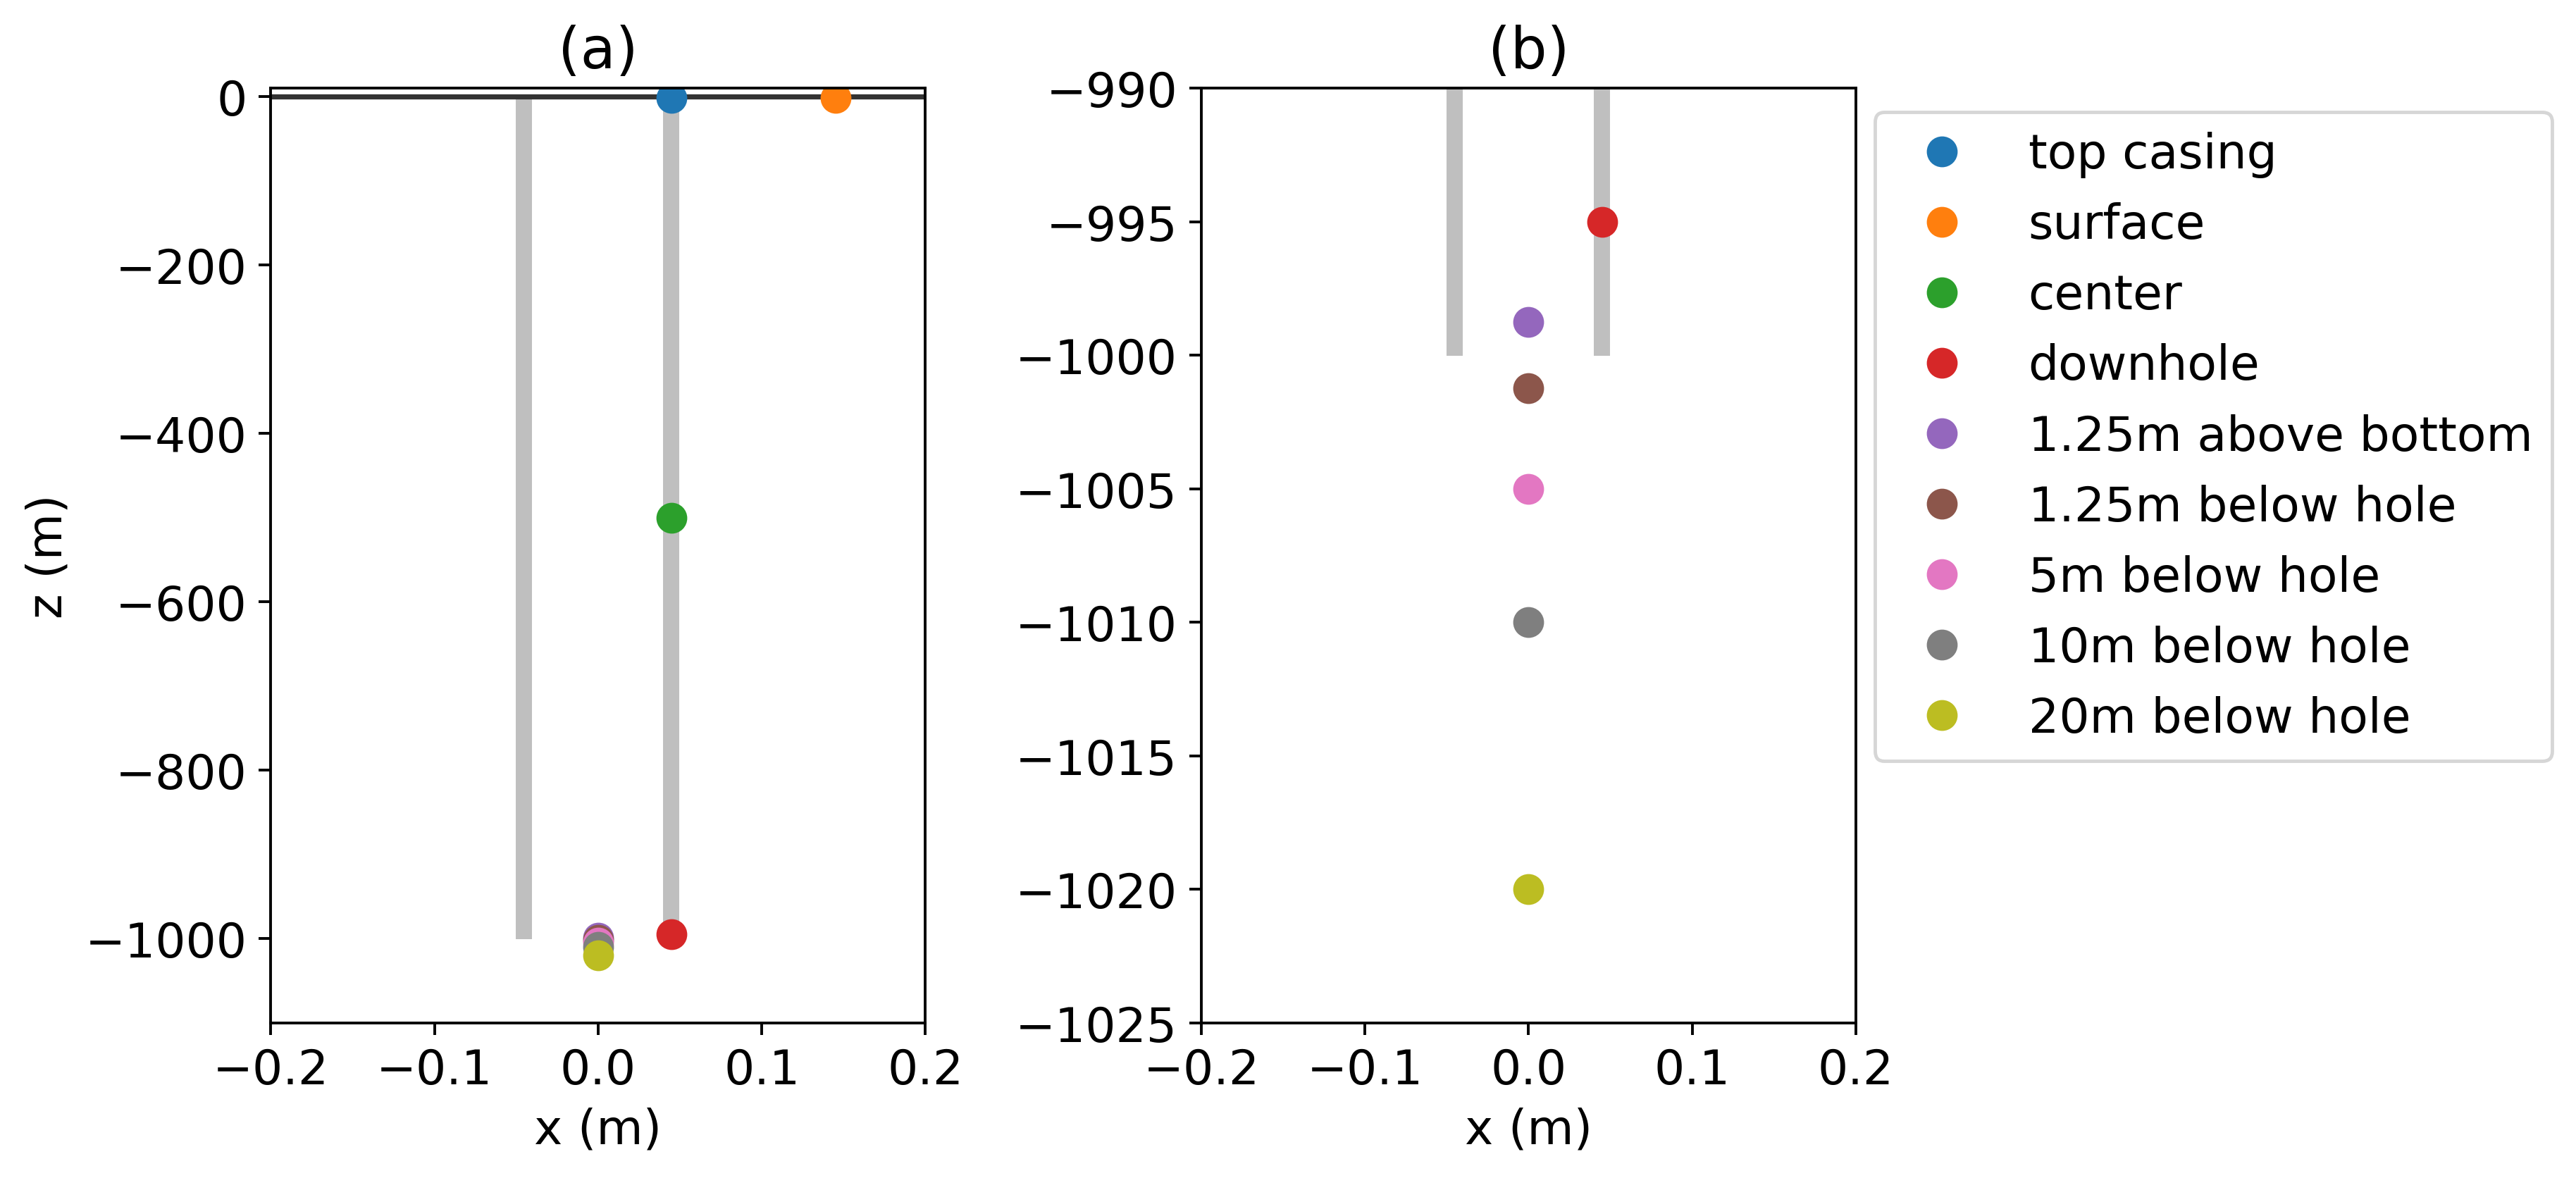
\includegraphics[width=\textwidth]{figures/electrode_location.png}
    \end{center}
\caption{
    Electrode locations to be compared. The top casing electrode (blue),
    centered electrode (green, 500m depth), and downhole electrode (red, 500m depth)
    are connected to the casing. The surface electrode (orange) is offset from the well
    by 0.1m. The remaining electrodes are positioned along the axis of the casing. Panel (a)
    shows the entire length of the casing, while (b) zooms in to the bottom of the casing
    to show the separation between the electrodes beneath the casing.
}
\label{fig:electrode_location}
\end{figure}


To assess the ability of each electrode configuration to excite a geologic target of interest, I will examine the current density in the formation. In Figure \ref{fig:electrode_location_currents}, I have plotted the amplitude of the current density along a vertical line (a) 25 m, (b) 50 m, and (c) 100 m radially offset from the well. In terms of survey design, we wish to choose a source location that maximizes the total current density within the depth region of interest. If the target is near the surface, we choose an electrode which is connected to the top of the casing, or near the casing at the surface. Interestingly, at depth, there is little distinction between these two scenarios. Thus, if one is limited to deploying electrodes at the surface, and for practical purposes, connecting infrastructure to the well-head presents a challenge, then grounding the electrode near the well still results in a survey that benefits from the well acting as a high-conductivity pathway to help deliver current to depth. If the aim however, is to excite a deeper target, we see that positioning the electrode downhole can significantly increase the current density delivered to that depth. For example, if we have a target near 500 m depth, positioning the electrode near that depth nearly doubles the current density as compared to an electrode at the surface. If a target is near the end of the well, between 800 m and 1000 m depth, then positioning an electrode near the end of the well triples the current density. This effect will be amplified if the well is lengthened, since we observe exponential decay of the currents carried along according to the conduction length (equation \ref{eq:conduction_length}).


\begin{figure}
    \begin{center}
    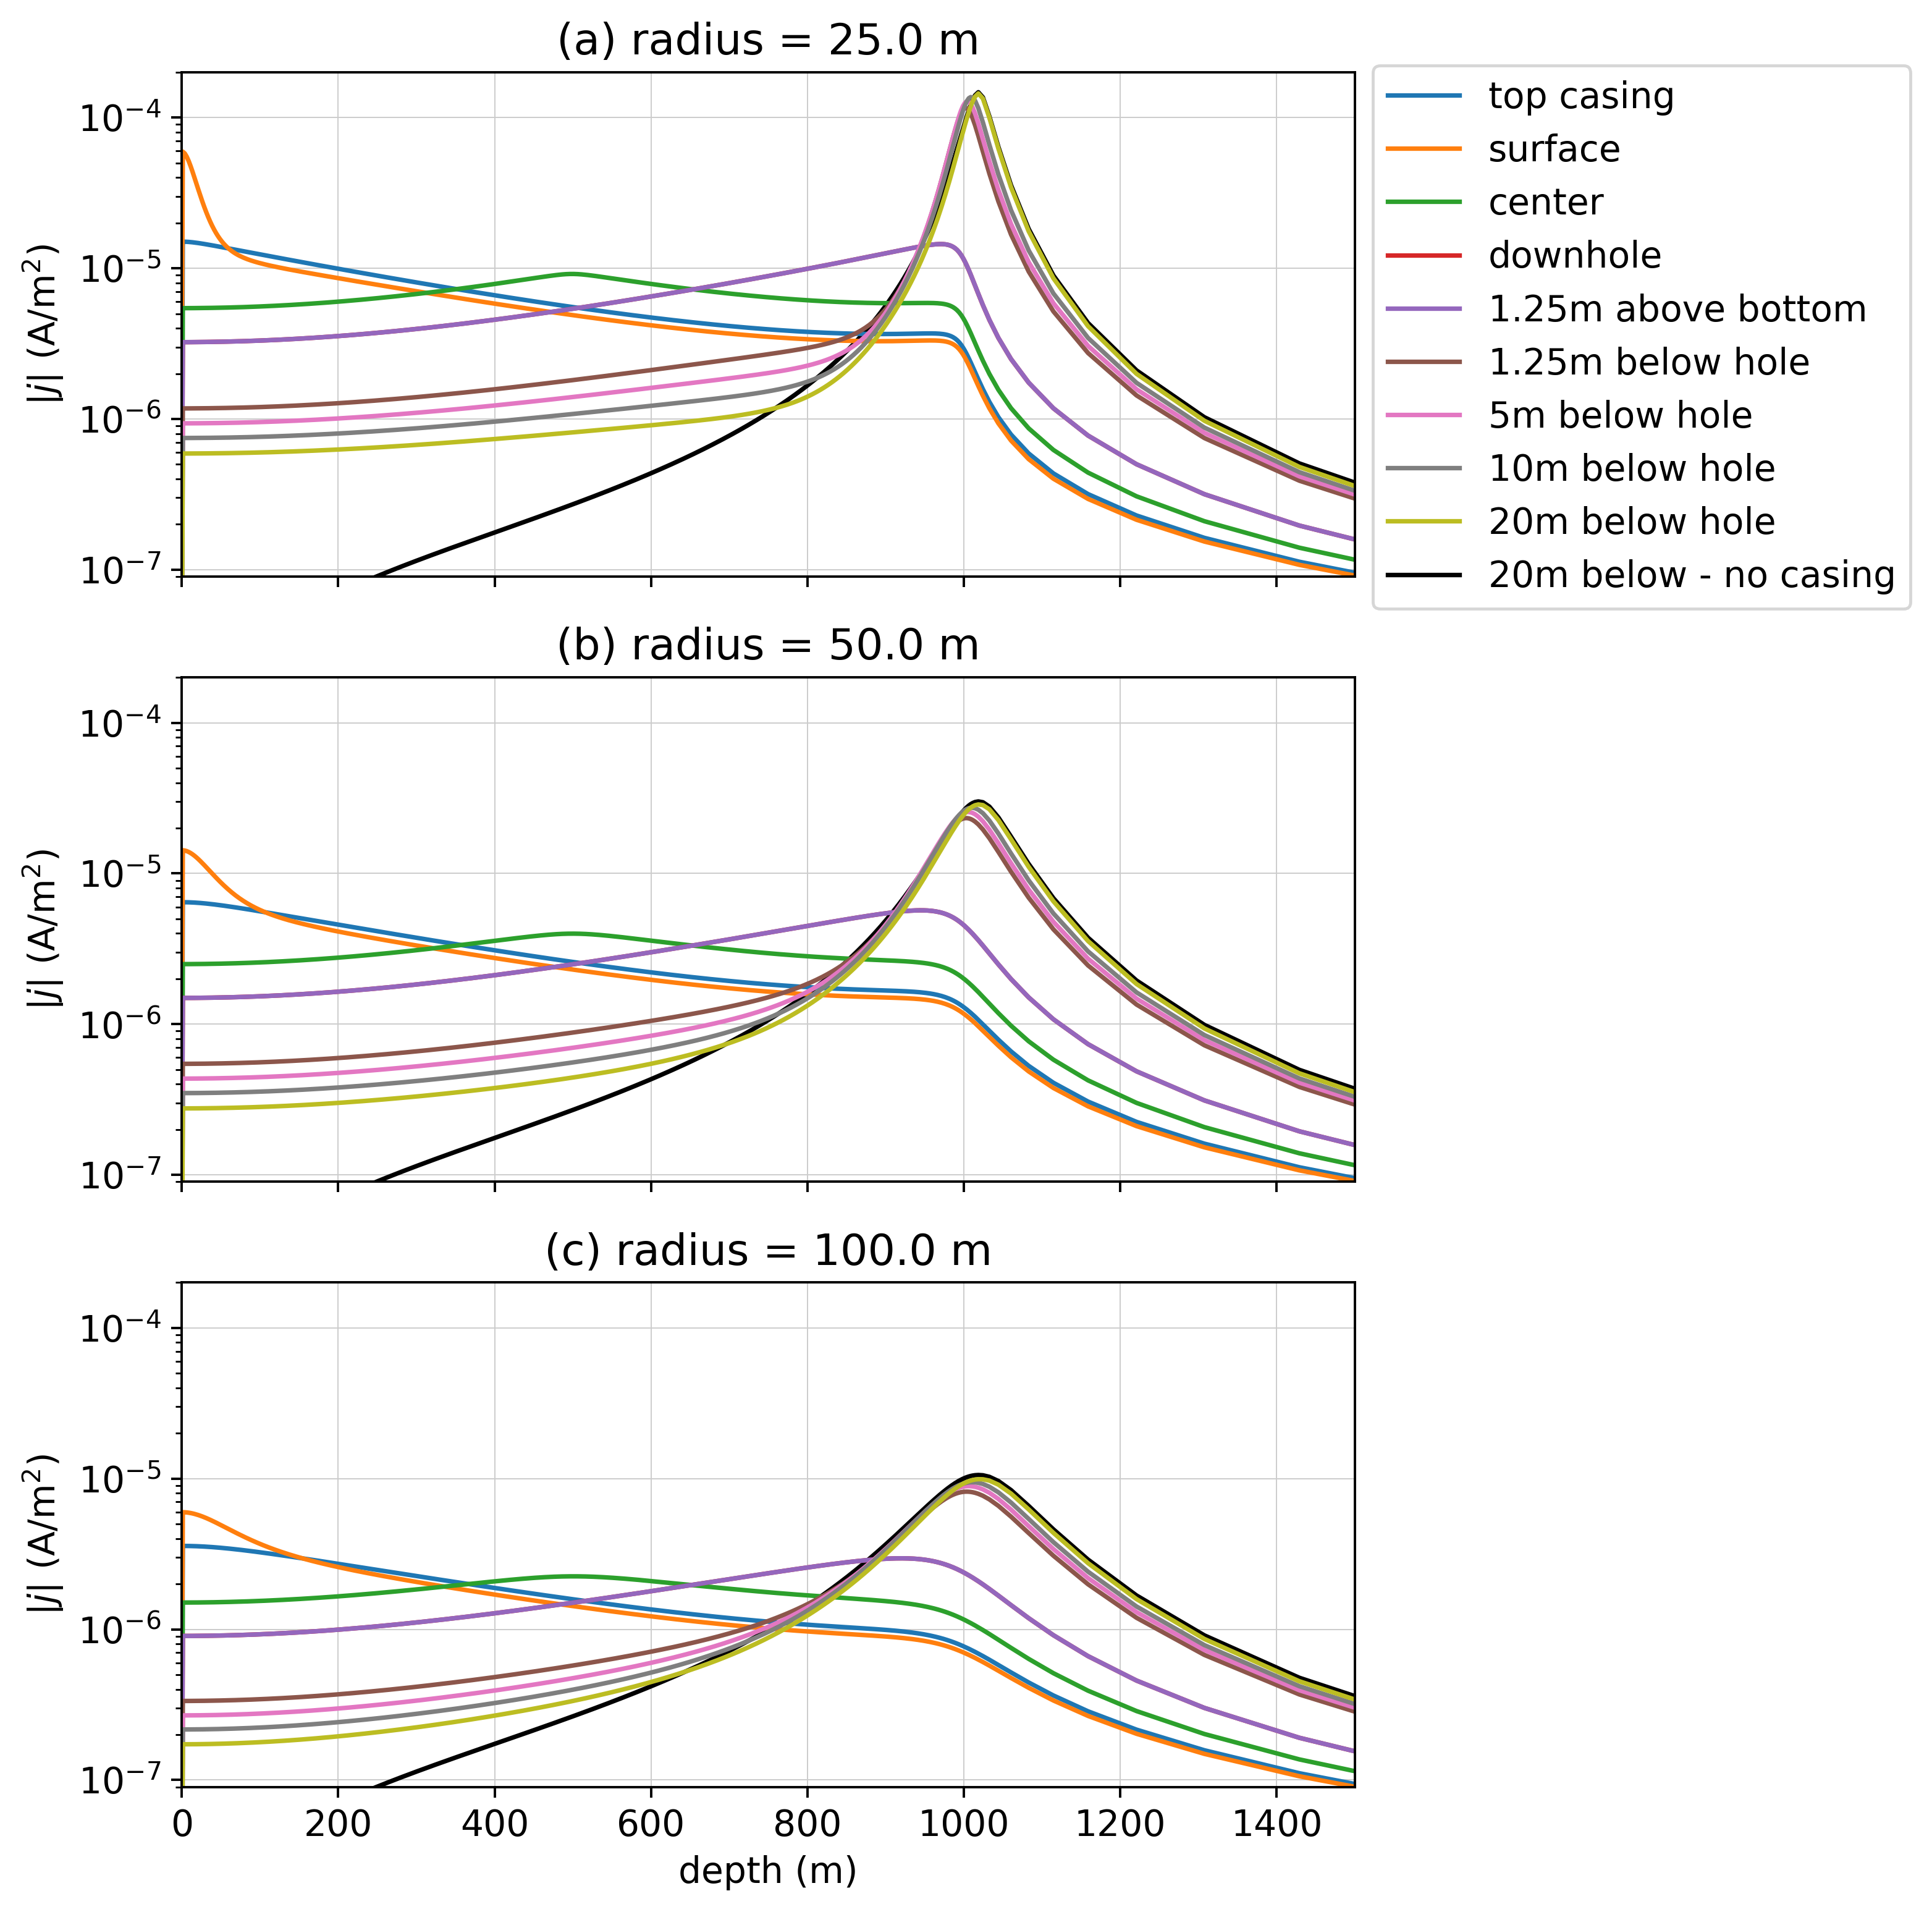
\includegraphics[width=0.8\textwidth]{figures/dc_casing/electrode_location_currents.png}
    \end{center}
\caption{
    Total current density along a vertical line offset (a) 25m, (b) 50m and (c) 100m
    from the axis of the casing, which extends
    from the surface (0m) to 1000m depth.
    The electrode locations correspond to those shown in Figure \ref{fig:electrode_location}.
    For reference, a simulation with an electrode 20m below the casing when there is no casing present
    is shown in black.
}
\label{fig:electrode_location_currents}
\end{figure}



\cite{Kaufman1990} pointed out that the difference between an electrode positioned along the axis of the casing and one coupled to the casing at depth is highly localized around the source, and thus is not an important distinction at the scales we consider for a geophysical imaging survey. I can test this numerically by comparing the currents arising from the electrode which is connected to the casing 5 m above the bottom of the casing (red in Figures \ref{fig:electrode_location} and \ref{fig:electrode_location_currents}), and the electrode positioned along the axis of the casing 1.25 m above the bottom of the casing (purple in Figures \ref{fig:electrode_location} and \ref{fig:electrode_location_currents}). Indeed, we see that the red and purple lines overlap for all offsets in Figure \ref{fig:electrode_location_currents}, indicating that both situations result in the same distribution of currents within the formation.

For electrodes beneath the casing, the distribution of currents is significantly different. For electrodes 1.25 m, 5 m, 10 m and 20 m below the pipe, we see that within $\sim$ 100 m above and below the electrode location, the currents are nearly symmetric, following the expected response of a point source. I have included a simulation with the electrode 20 m below the pipe when there is no casing present; this is shown in black in Figure \ref{fig:electrode_location_currents}. The main difference between the distribution of currents for each of these scenarios is the reduction in current density in the top 1000 m, with increasing electrode depth; as the electrode is moved deeper, less current is channeled into the casing. \cite{Schenkel1990} noted that for electrodes positioned beneath a well, if the electrode is more than 100 casing diameters beneath the casing, then the casing has little impact on the fields below or far from the pipe. The current is much more localized if the electrode is beneath the casing, and thus if a target is beneath or very near the end of the well, then it is advantageous to position the electrode beneath the well.

Not surprisingly, if the source electrode can be positioned near the depth region of interest, the current density delivered to that region is larger. Numerical experiments show that the position of the return electrode makes minimal impact on the currents at depth. However, if the return electrode is within tens of meters of the well, the near surface currents are significantly altered. This is consistent with our observations in section \ref{sec:casing_integrity}, where I showed that the return electrode location has little impact on the magnitude of the secondary signals, but its position alters the geometry of the source fields and this can be used to reduce coupling of receivers to the primary field.


\subsection{Target properties}
The physical property contrast between the target and the background, the target's geometry and proximity to the well, all influence our ability to observe its impact on the data we measure. The purpose of this section is to explore the impact of these factors on the excitation and detection of the target. In the first example, I examine the role of the conductivity of a cylindrical target which is in contact with  the well. The second example is again a cylindrically symmetric co-axial disc target but there is a gap between the casing and the target. The final example is fully 3D; the target is a block and I look at the excitation as a function of the distance of a block from the well.

\subsubsection{Target in contact with the well}
First, I consider a cylindrical target that is in contact with the well. \cite{Schenkel1994} examined such a scenario for a conductive target (e.g. a steam injection or water flood) in a mis-\`a-la-masse type experiment where a source electrode is connected to the casing at the same depth as the center of the target. They considered a cross-well experiment with potential electrodes in an offset, uncased well, and compared two scenarios for the source well: one in which the source well is an open-hole, and the second in which it was cased. They demonstrated that the casing enhances the response, and thus the data sensitivity to the target, as compared to an experiment where current is injected directly into the target and no casing is present. In this example, I build upon those findings and examine the role of the conductivity of the target on our ability to excite it as well as the impact on the data if the target is not directly in contact with the well.

The model I use is a 1 km casing in a half-space with a target. The target extends 25 m vertically and has a 25 m radius and the depth to its top is 900 m. The model is cylindrically symmetric and thus we expect that the secondary electric field at the surface due to the target will be purely radial. As such, I apply the lessons learned from the casing integrity example and use the return electrode to reduce coupling with the primary field along a line perpendicular to the source. I position the return electrode 500 m from the well-head and compare both top-casing and down-hole source electrode locations.

We begin by examining the physical behavior governing the DC response of a conductive and resistive target. Figure \ref{fig:target_physics} shows the (a) conductivity model, and resultant: (b) current density, (c) charge density, and (d) electric fields for a conductive target ($10$ S/m, top row) and a resistive target ($10^{-3}$ S/m, bottom row) in a down-hole experiment where the source electrode is positioned at the center of the target. The extent of the steel-cased well is noted by the vertical black line in panel (a). For the conductive target, we see an accumulation of positive charges along the radial and vertical boundaries of the target. This is consistent with currents that have been channeled into the conductor and exit into a more resistive background. Conversely, for the resistive target, we see an accumulation of negative charge on the radial boundary, consistent with current moving from a resistive region to a more conductive material. We also notice some positive charge accumulation on the top and bottom boundaries of the target; some of the currents deflected around the resistor do enter from the top and bottom, resulting in an accumulation of positive charge. This is not observed in a traditional mis-\`a-la-masse experiment, where a point source is positioned within the target. Figure \ref{fig:uncased_target_physics} shows the current density, charges and electric fields for a mis-\`a-la-masse experiment in which no steel cased well is present.

\begin{figure}
    \begin{center}
    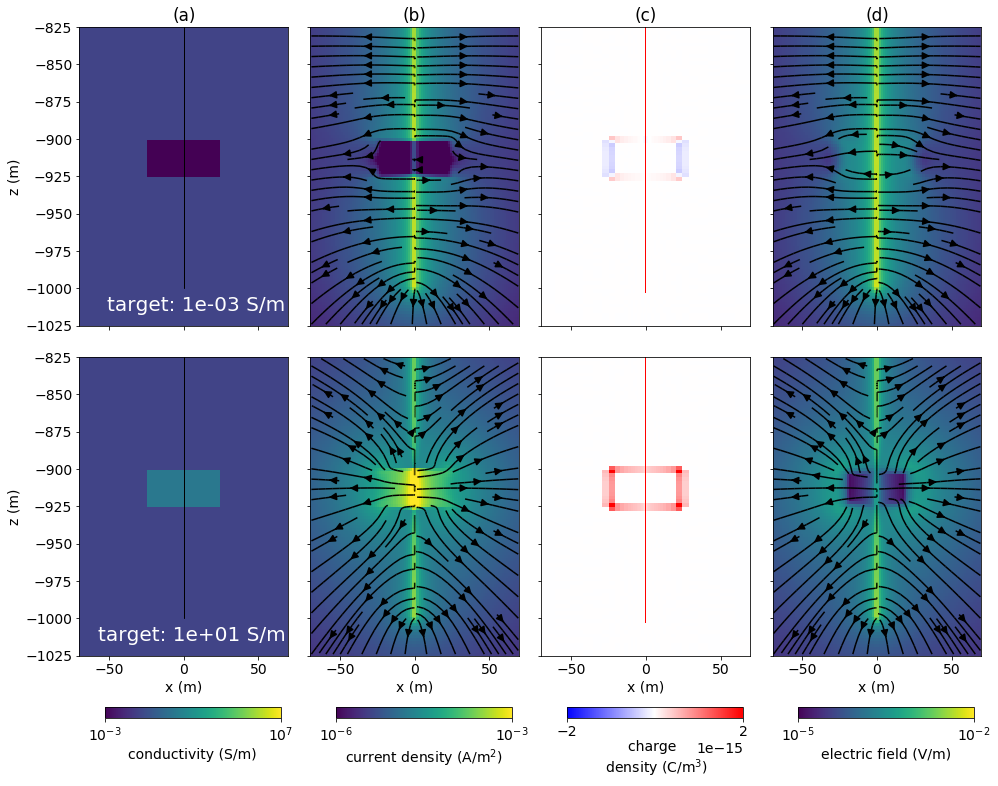
\includegraphics[width=\textwidth]{figures/dc_casing/target_physics.png}
    \end{center}
\caption{
    Cross section showing: (a) electrical conductivity, (b) current density, (c) charge density, and
    (d) electric field for a DC resistivity experiment with a resistive target (top) and a conductive target
    (bottom). The positive electrode is positioned in the casing at the 912.5 m depth.
    The casing is shown by the black line that extends to 1 km
    depth in panel (a).
}
\label{fig:target_physics}
\end{figure}



\begin{figure}
    \begin{center}
    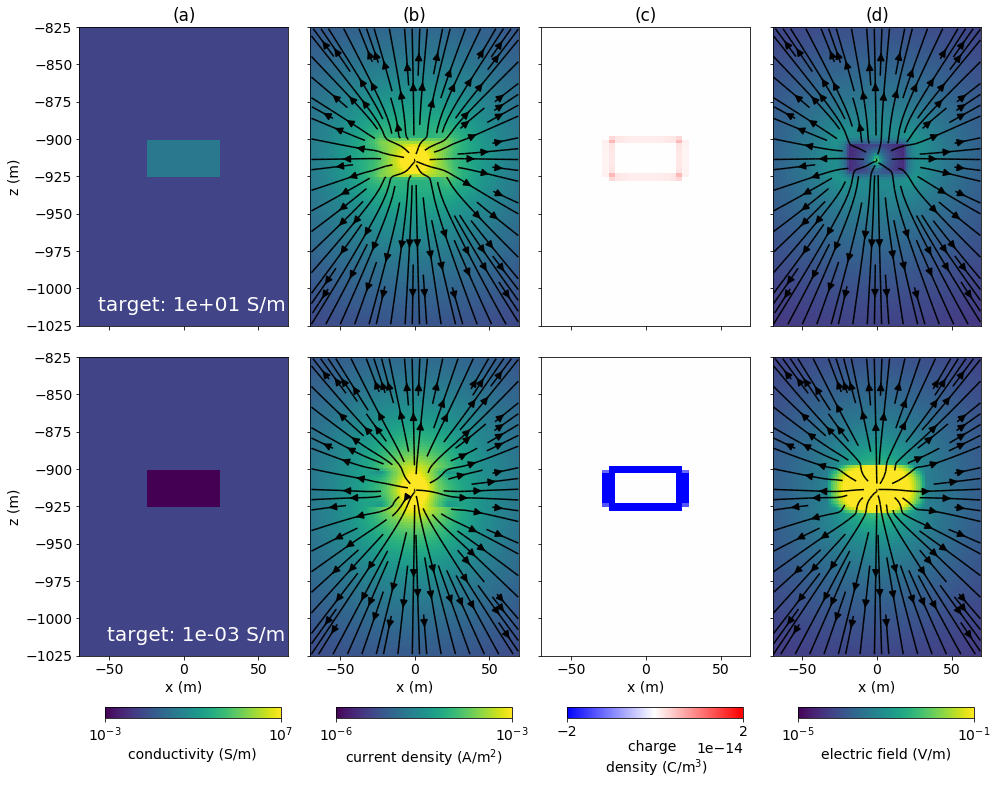
\includegraphics[width=\textwidth]{figures/dc_casing/uncased_target_physics.png}
    \end{center}
\caption{
    Cross section showing: (a) electrical conductivity, (b) current density, (c) charge density, and
    (d) electric field for a DC resistivity experiment with a conductive target (top) and a resistive target
    (bottom). The positive electrode is positioned at 912.5m depth.
    No casing is included in this simulation. Note that the colorbars for the charge density (c) and electric field (d)
    are different than those used in Figure \ref{fig:target_physics}. For the resistive target, the colorbar is saturated,
    the charge density over the resistive target is on the order of $10^{-13}$ C/m$^3$.
}
\label{fig:uncased_target_physics}
\end{figure}


In a DC experiment, the electric field response we measure is a result of the distribution of charges within the domain. As a metric for quantifying excitation, I integrate the secondary charge over this depth interval containing the target. In Table \ref{tab:target_charge}, I show the secondary charge integrated over the depth interval containing the target; the secondary charge on the casing within this region is included in the calculation. To examine how the charge relates to the electric field data, I have plotted (a) total radial electric field, (b) secondary radial electric field (with respect to a primary that includes the casing in a halfspace), and (c) the secondary radial electric field as a percentage of the primary for a down-hole source and similarly for a top-casing source (d, e, f) in Figure \ref{fig:target_electric_fields}. I adopt the same noise floor and percent threshold as in the casing integrity examples ($10^{-7}$ V/m and $20\%$, respectively). For time-lapse surveys where a baseline survey has been taken and the background is well-characterized, this threshold could likely be reduced. The black line in panels (a) and (d) corresponds to the baseline model in which no target is present; each of the colored lines corresponds to a different target conductivity as indicated in the legend.



\begin{table}
\centering
    \caption{Integrated secondary charge over a target adjacent to the casing, as shown in Figure \ref{fig:target_physics}.}
    \begin{tabular}[htb]{| r | r | r |}
        \hline
                                           & \multicolumn{2}{|c|}{\textbf{integrated secondary charge (C)}} \\
        \textbf{target conductivity (S/m)} & \textbf{downhole source} & \textbf{top-casing source} \\
        \hline
        1e-03 & -4.24e-12 & -1.08e-12 \\
        1e-02 & -3.82e-12 & -9.68e-13 \\
        1e-01 & 0.00e+00 & 0.00e+00 \\
        1e+00 & 1.75e-11 & 4.46e-12 \\
        1e+01 & 3.26e-11 & 8.28e-12 \\
        \hline
    \end{tabular}
    \label{tab:target_charge}
 \end{table}




\begin{figure}
    \begin{center}
    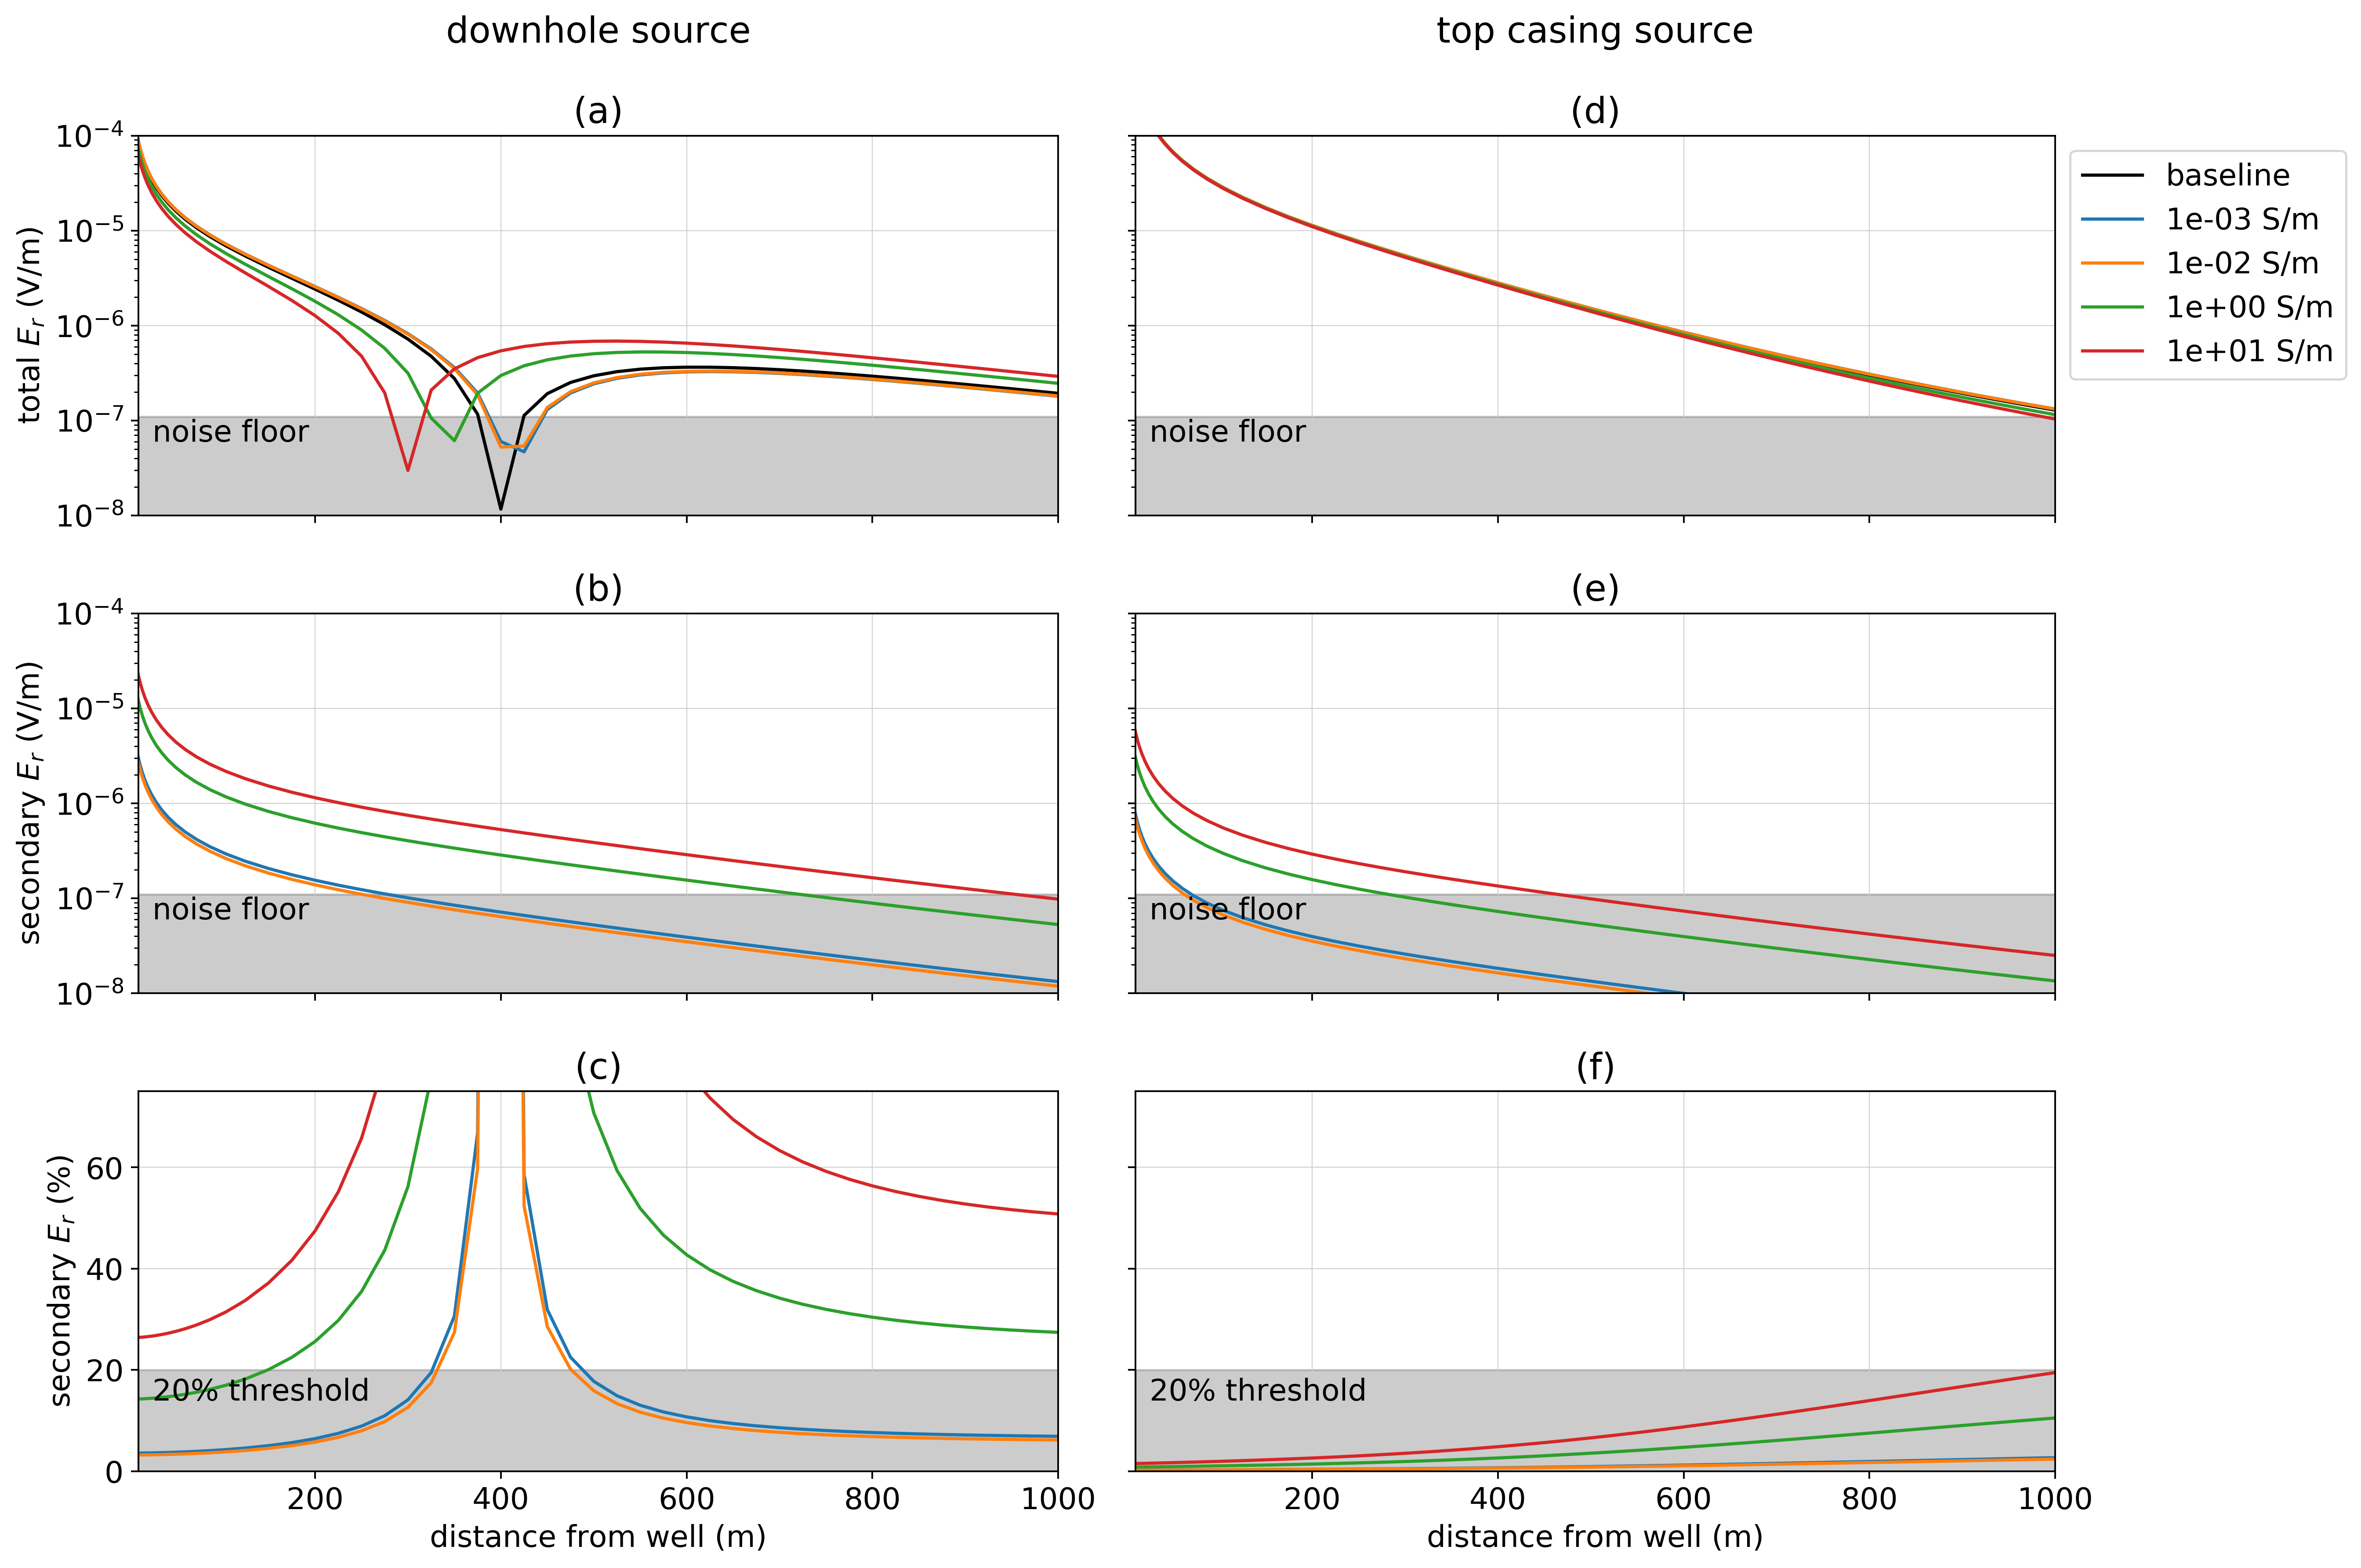
\includegraphics[width=\textwidth]{figures/dc_casing/target_electric_fields.png}
    \end{center}
\caption{
    Radial electric field at the surface as the conductivity of a cylindrical target, in contact with the well,
    is varied. The target has a radius of 25m and extends in depth from 900m to 925m. The return electrode
    is on the surface, 500m from the well and data are measured along a line perpendicular to the source.
    The panels on the left show
    (a) the total electric field, (b) the secondary electric field with respect to a primary that does not include the target,
    and (c) the secondary electric field as a percentage of the primary for a survey in which the positive electrode is
    positioned downhole at 912.5m depth. The panels on the right similarly show (d) the total electric field, (e) the
    secondary electric field, and (f) the secondary electric field as a percentage of the primary for a top-casing experiment.
}
\label{fig:target_electric_fields}
\end{figure}


First, we examine the impact of the conductivity of the target and notice that there is an asymmetry between secondary charge on conductive targets and resistive targets. For a 1 S/m target, which is one order of magnitude more conductive than the background, the integrated secondary charge is $1.75 \times 10^{-11}$ C, while for a $1\times10^{-2}$ S/m target, which is one order of magnitude more resistive than the background, the integrated secondary charge is $-3.82 \times 10^{-12}$ C for the downhole casing experiment. Thus, there is a factor of 4.6 between the magnitude of the secondary charge for these targets; this is equivalent to the ratio we see between the secondary electric field measurements at the surface observed in Figure \ref{fig:target_electric_fields}b. When also considering the influence of the primary electric field on our ability to detect a target, we see that for a down-hole casing experiment, the conductive targets are detectable; they both have a significant region where the secondary is above the noise floor and the secondary comprises a significant percentage of the primary. The resistive targets, however, are not. Although within 200 m of the well, the secondary signal is above the noise floor, this also corresponds to where the primary field is large; the percent threshold would need to be reduced to less than 5\% in order to have confidence in the signals due to the resistive targets.

When comparing the downhole source to the top-casing source experiments for a fixed conductivity, there is a factor of 3.9 between the integrated secondary charge shown in \ref{tab:target_charge}; this is reflected in the secondary electric field data in Figure \ref{fig:target_electric_fields}b \& e.  For the top-casing experiment, none of the targets is detectable. There are two factors that make this a more challenging experiment than the downhole scenario: (1) less current is available to excite the target, as reflected in Table \ref{tab:target_charge} and (2) the primary field is stronger at the receivers (200 m from the well the primary field has an amplitude of $10^{-5}$ V/m, while for the down-hole source experiment, the primary has an amplitude of $2 \times 10^{-6}$ V/m). Addressing the excitation of the target requires that the source electrode be positioned downhole, closer to the target. The second point may be overcome if receivers can be positioned closer to the target, for example within an adjacent borehole.

In summary, the integrated secondary charge provides a metric for a survey's ability to excite a target, and shows that conductive targets are easier to excite than resistive targets. As expected, if the source electrode can be positioned near the target, excitation is enhanced. This also has the added benefit of reducing the strength of the primary electric field at the surface, as compared to a top-casing survey; this  increases the potential for detecting a target with surface-based receivers. In the next section, I examine the significance of the electrical connection between the casing and the target.

\subsubsection{Target not in contact with the well}

How significant is the electrical connection between the casing and the target for our ability to excite a response? To examine this, I introduce a small gap equal to the thickness of the casing (1 cm) between the casing and the target. This has negligible effect on the volume of the target, but it changes the electrical characteristics of the problem. Consider a conductive target; if it is in-contact with the well, we are effectively conducting a mis-\`a-la-masse experiment, and the conductor will have a net positive charge. When the target is isolated from the casing, the total charge on the target must be zero, and thus dipolar effects, in which negative charges build up on the inner interface of the cylinder target and positive charges build up on the outer interface of the target, will be the source of our signal. This is demonstrated in Figure \ref{fig:offset_target_physics}.

\begin{figure}
    \begin{center}
    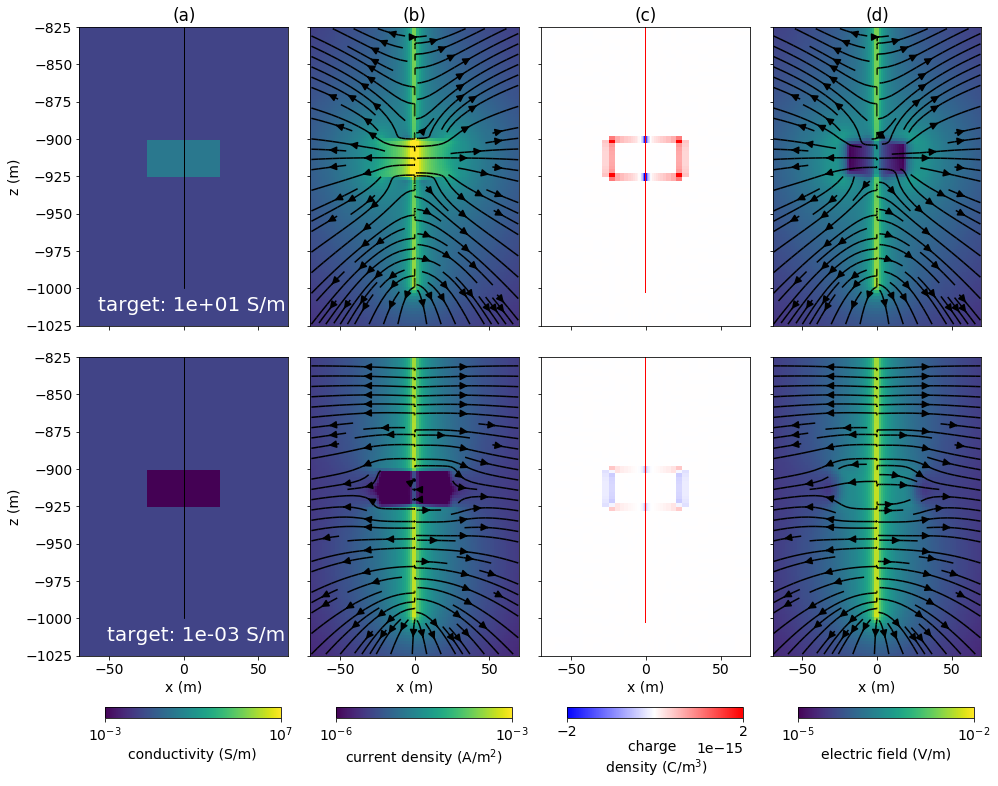
\includegraphics[width=\textwidth]{figures/dc_casing/offset_target_physics.png}
    \end{center}
\caption{
    Cross section showing: (a) electrical conductivity, (b) current density, (c) charge density, and
    (d) electric field for a DC resistivity experiment with a conductive target (top)
    and a resistive target (bottom) which is not in contact with the well.
    The positive electrode is positioned in the casing at the 912.5m depth.
    The casing is shown by the black line that extends to 1km
    depth in panel (a).
}
\label{fig:offset_target_physics}
\end{figure}


The corresponding secondary charge integrated over the target depth and radial electric field data are shown in Table \ref{tab:offset_charge} and Figure \ref{fig:offset_electric_fields}. For comparison, the data resulting from the target in contact with the well are plotted in the dashed, semi-transparent lines. While there is little difference in the integrated secondary charge or the electric field measurements for the resistive targets, we see that there is a factor of 1.3 difference (i.e. 30\%) between the integrated secondary charges and correspondingly, the secondary electric fields, from a 10 S/m target in contact with the well versus not. Similarly, there is a factor of 1.2 between a 1 S/m target in contact with the well versus not for both the downhole and top-casing sources. Increasing the gap between the target and the casing decreases the integrated charge and correspondingly reduces the secondary electric field at the surface. The integrated secondary charge for a 10 S/m target with a 10 cm gap between the target and casing in a downhole source experiment is $1.7 \times 10^{-11}$ C, which is a factor of 2.2 smaller than the connected target; correspondingly the electric field data at the surface are reduced by a factor of 2.2 as compared to the connected target. Thus, a direct, electrical connection between the target and the well in which we connect the source is preferable for exciting and detecting conductive targets. In the next section, I further examine the impact of the separation between the target and casing.


\begin{table}
\centering
    \begin{tabular}[htb]{| r | r | r |}
        \hline
                                           & \multicolumn{2}{|c|}{\textbf{integrated secondary charge (C)}} \\
        \textbf{target conductivity (S/m)} & \textbf{downhole source} & \textbf{top-casing source} \\
        \hline
        1e-03 & -4.24e-12 & -1.08e-12 \\
        1e-02 & -3.80e-12 & -9.64e-13 \\
        1e-01 & 0.00e+00 & 0.00e+00 \\
        1e+00 & 1.49e-11 & 3.79e-12 \\
        1e+01 & 2.51e-11 & 6.39e-12 \\
        \hline
    \end{tabular}
    \caption{Integrated secondary charge over a target that is not electrically connected to the casing, as shown in Figure \ref{fig:offset_target_physics}.}
    \label{tab:offset_charge}
 \end{table}




\begin{figure}
    \begin{center}
    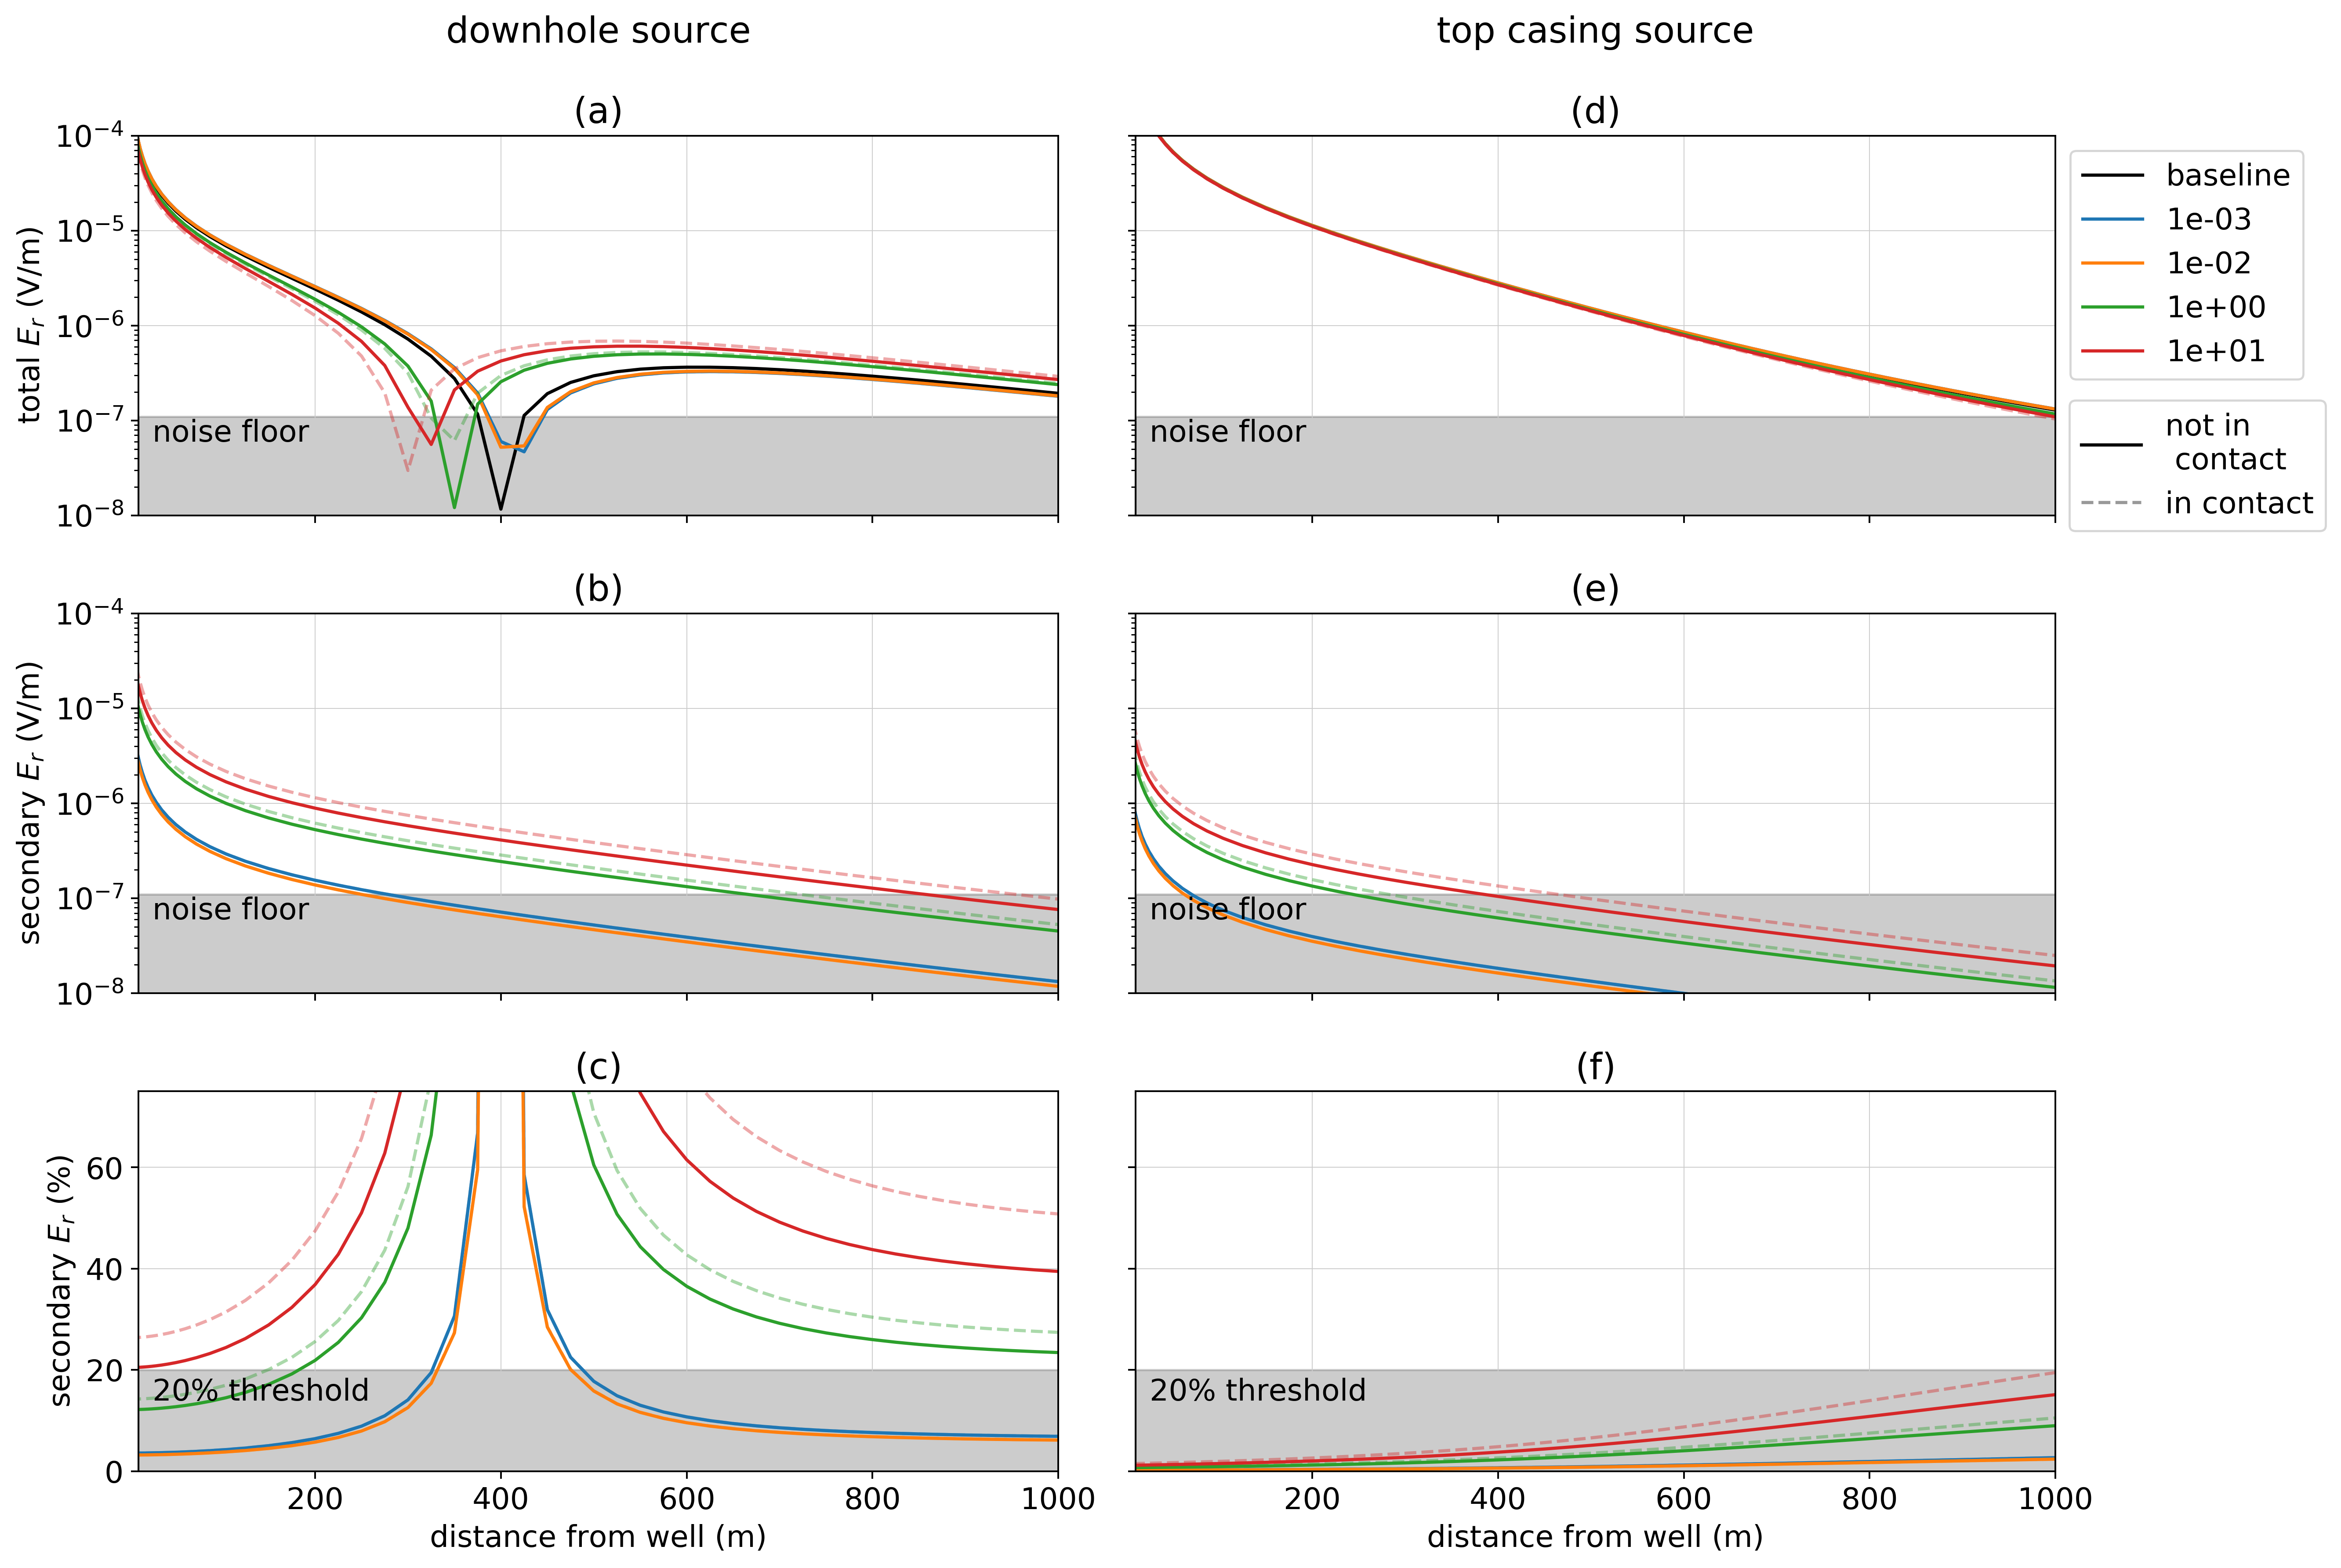
\includegraphics[width=\textwidth]{figures/dc_casing/offset_electric_fields.png}
    \end{center}
\caption{
    Radial electric field at the surface as the conductivity of a cylindrical target, which is not contact with the well,
    is varied. The target has a radius of 25m and extends in depth from 900m to 925m. The return electrode
    is on the surface, 500m from the well and data are measured along a line perpendicular to the source.
    The panels on the left show
    (a) the total electric field, (b) the secondary electric field with respect to a primary that does not include the target,
    and (c) the secondary electric field as a percentage of the primary for a survey in which the positive electrode is
    positioned downhole at 912.5m depth. The panels on the right similarly show (d) the total electric field, (e) the
    secondary electric field, and (f) the secondary electric field as a percentage of the primary for a top-casing experiment.
    The data shown in Figure \ref{fig:target_electric_fields}, for the target in contact with the well,
    are plotted in the dashed, semi-transparent lines for reference.
}
\label{fig:offset_electric_fields}
\end{figure}




\subsubsection{Target offset from the well}

The examples thus far have focused on a particular geometry where the target is symmetric about the well and is either connected or not. The more general case is where there is a target located anywhere in the medium and we wish to use DC or EM to characterize it. For example, in some scenarios, instrumenting a well for a geophysical survey may not be possible if it is also actively being used for an injection. Using another well, offset from the injection well, may then be preferable for positioning electrodes. In such circumstances, the physical property model is fully 3D and there are more factors that influence our ability to excite the target; in addition to the conductivity and geometry of the target, the distance between the well where the source electrode is positioned is now relevant. To address these potential applications, I examine a fully 3D scenario in which a target block is located away from the source well. Our primary goal is to compare relative excitations that arise from using different survey parameters. It is sufficient to evaluate an electric dipole moment of the target that is evaluated with a Born approximation \citep{Born1933}.

For a target offset from the pipe, we expect the secondary response due to that target to be dipolar. Thus, a natural proxy for excitation is the dipole moment of the target. I will adopt a Born-approximation approach to quantify the excitation and take the norm of the integrated anomalous current density over the target volume, that is,
\begin{equation}
    \begin{split}
    m & = \left|\left| \int \vec{j}_a ~ dV \right|\right| \\
                      & = \left|\left| \int \sigma_s \vec{e}_p ~ dV \right|\right|
    \label{eq:excitation}
    \end{split}
\end{equation}

where $\sigma_s = \sigma - \sigma_p$ is the secondary conductivity (the difference between the conductivity of the target and the conductivity of the background), $\vec{e}_p$ is the primary electric field (the electric field due to the source, casing, and half-space background), and $\vec{j}_a$ is the anomalous current density which is non-zero only over the volume where the target is located.

The target I consider is 50 m wide in both horizontal dimensions and is 25 m in height. Its top is at 900 m depth, as in the previous examples. I will examine both downhole source and top-casing experiments. A depth slice showing the primary electric field for the downhole electrode is shown in Figure \ref{fig:primary_3D}; the return electrode is on the surface at $x=$-500 m, $y=$0 m. The three different target positions relative to the borehole are outlined in white. The solid line shows the target which is inline with the return electrode, the dashed is $90^\circ$ from the source electrode and the dotted line shows the target which is $180^\circ$ from the return electrode. I vary the distance from the well to the target and have plotted the Born-approximated dipole moment for four different target conductivities in Figure \ref{fig:excitation_3D} for (a) a downhole experiment, and (b) a top-casing experiment. The offset is calculated from the center of the well to the nearest edge of the target that is excited by a downhole source. As before, conductive targets are much easier to excite than resistive targets, and for a given conductivity, a downhole source provides greater excitation than a top-casing source. Naturally, as the target is moved further from the well, the geometric decay of source fields reduces our ability to excite the target. Positioning the return electrode along the same azimuth as the target acts to mitigate some of these effects for targets that are at distances greater than 200 m from the well, while for targets nearer to the well, the return electrode location has little effect on the excitation.


\begin{figure}
    \begin{center}
    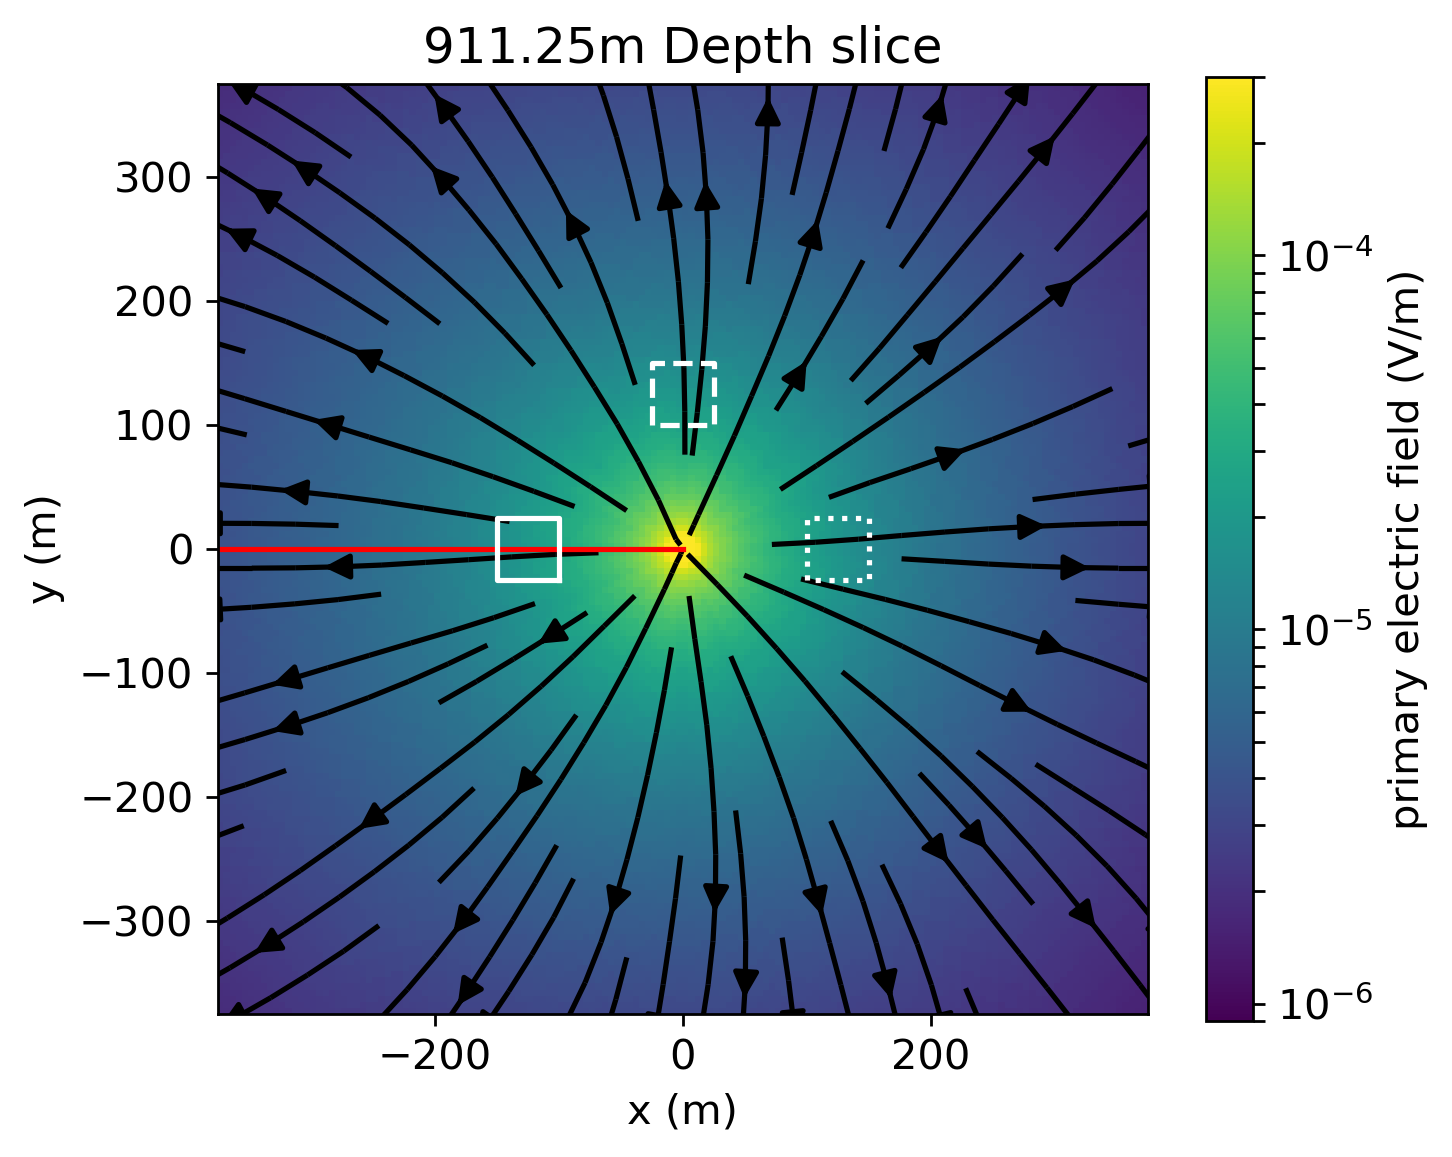
\includegraphics[width=0.6\textwidth]{figures/dc_casing/primary_3D.png}
    \end{center}
\caption{
    Depth slice showing the primary electric field due to a downhole
    electrode and a return electrode located on the surface at x=-500m, y=0m. The red line indicates the
    azimuth of the source.
    We examine the 3 different target azimuths shown by the white outlines.
    The solid line indicates the target inline with the source,
    the dashed is $90^\circ$ from the source line, and the dotted line is $180^\circ$ from the source line.
}
\label{fig:primary_3D}
\end{figure}



\begin{figure}
    \begin{center}
    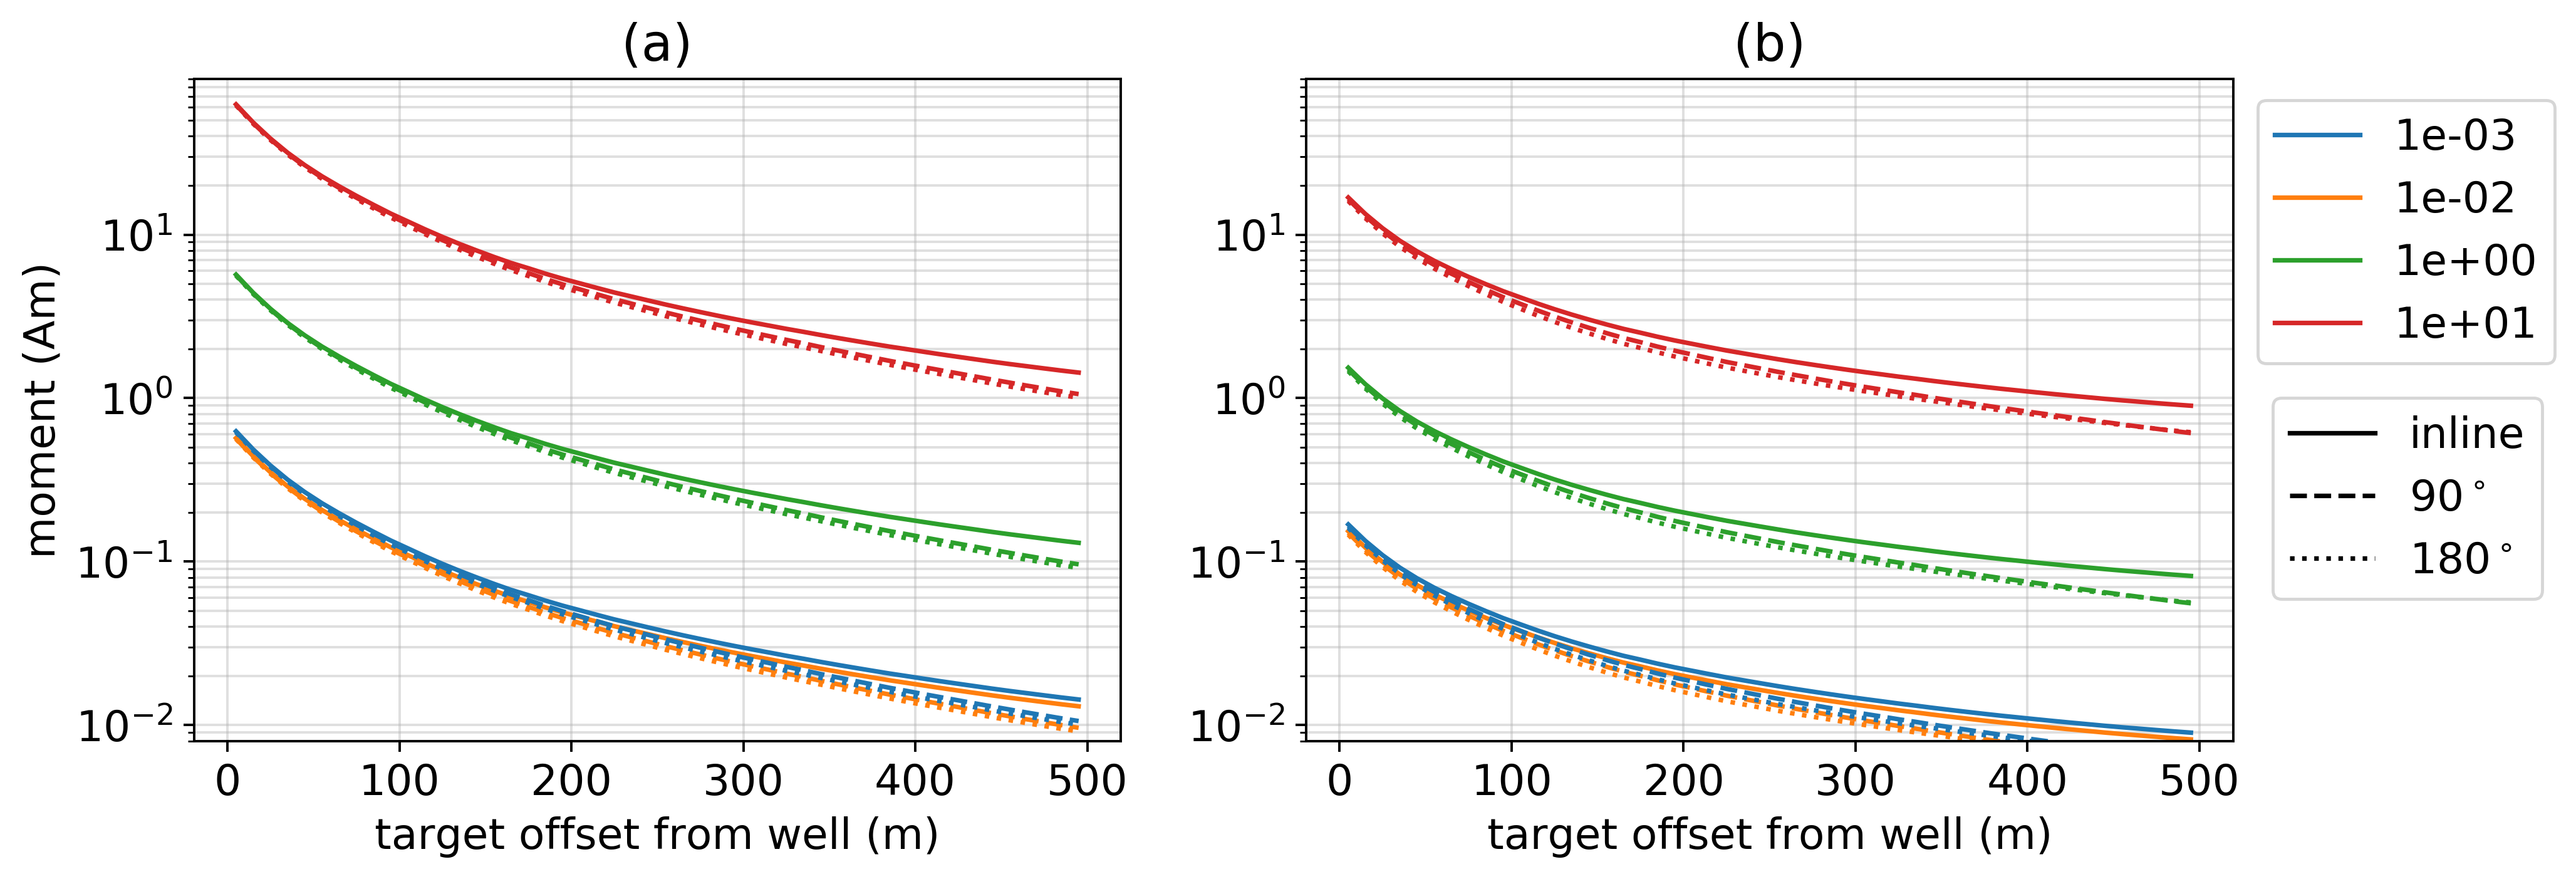
\includegraphics[width=\textwidth]{figures/dc_casing/excitation_3D.png}
    \end{center}
\caption{
    Integrated anomalous current density (excitation), as defined in equation \ref{eq:excitation},
    for a 50 m $\times$ 50 m $\times$ 25 m target at 900 m depth in a DC experiment with the positive electrode
    (a) downhole at 912.5 m depth, and (b) a top-casing electrode. The return electrode is positioned on the
    surface 500 m from the well. Each line color indicates a different target-conductivity. The different line
    styles correspond to different target azimuths relative to the plane of the source electrodes and correspond
    to those show in Figure \ref{fig:primary_3D}. The solid line indicates a target inline with the source,
    the dashed is $90^\circ$ from the source, and the dotted line is $180^{\circ}$ from the source. Offset is
    calculated from the center of the well to the edge of the target closest to the well.
}
\label{fig:excitation_3D}
\end{figure}


The next step to consider is detection of the secondary response due to this target. Consistent with the Born-approximation approach, I simulate the target as a dipole with a moment computed with equation \ref{eq:excitation} and compare the secondary electric field data at the surface for models with, and without, the casing. For this example, I select the model of a conductive target (10 S/m) with center 50 m offset from the well. The target is along a line $90^\circ$ from the source (e.g. along the same line as the dashed-outline in Figure \ref{fig:primary_3D}). This gives a dipole moment of 38 Am for the target. The electric field data, measured along the same line as the target, are shown in Figure \ref{fig:detectability_dipole}. The secondary response with the casing is shown in blue, and the response of the same dipole in a half-space is shown in orange. The secondary response due to the dipole in a half-space falls below the $10^{-7}$ V/m noise floor for all offsets, whereas, when the casing is included, the secondary response is above the noise floor until beyond offsets of 600 m from the well. The casing not only helps excite a target, as was demonstrated in \cite{Schenkel1994}, it also provides a conductive pathway for the secondary currents, thus increasing the secondary signal observed at the surface; this was similarly noted in \cite{Yang2016}. In the model with the casing, the secondary signal comprises a significant percentage of the primary between offsets of $\sim$ 200 m and $\sim$ 650 m, providing a window between 200 m and 600 m where the secondary electric field is above the noise floor and comprises a significant percentage of the primary.

If I move the target further from the well, positioning its center 75 m from the well, then the dipole moment is reduced to 24 Am. If I use the criterion that the secondary electric field must be above the noise floor and be at least 20\% of the primary field, then the region over which we can expect to collect data is reduced to a 50 m window between 300 m and 350 m offset from the well. For this given survey, then, we can consider $\sim$ 25 Am as a threshold for detectability of a target.



\begin{figure}
    \begin{center}
    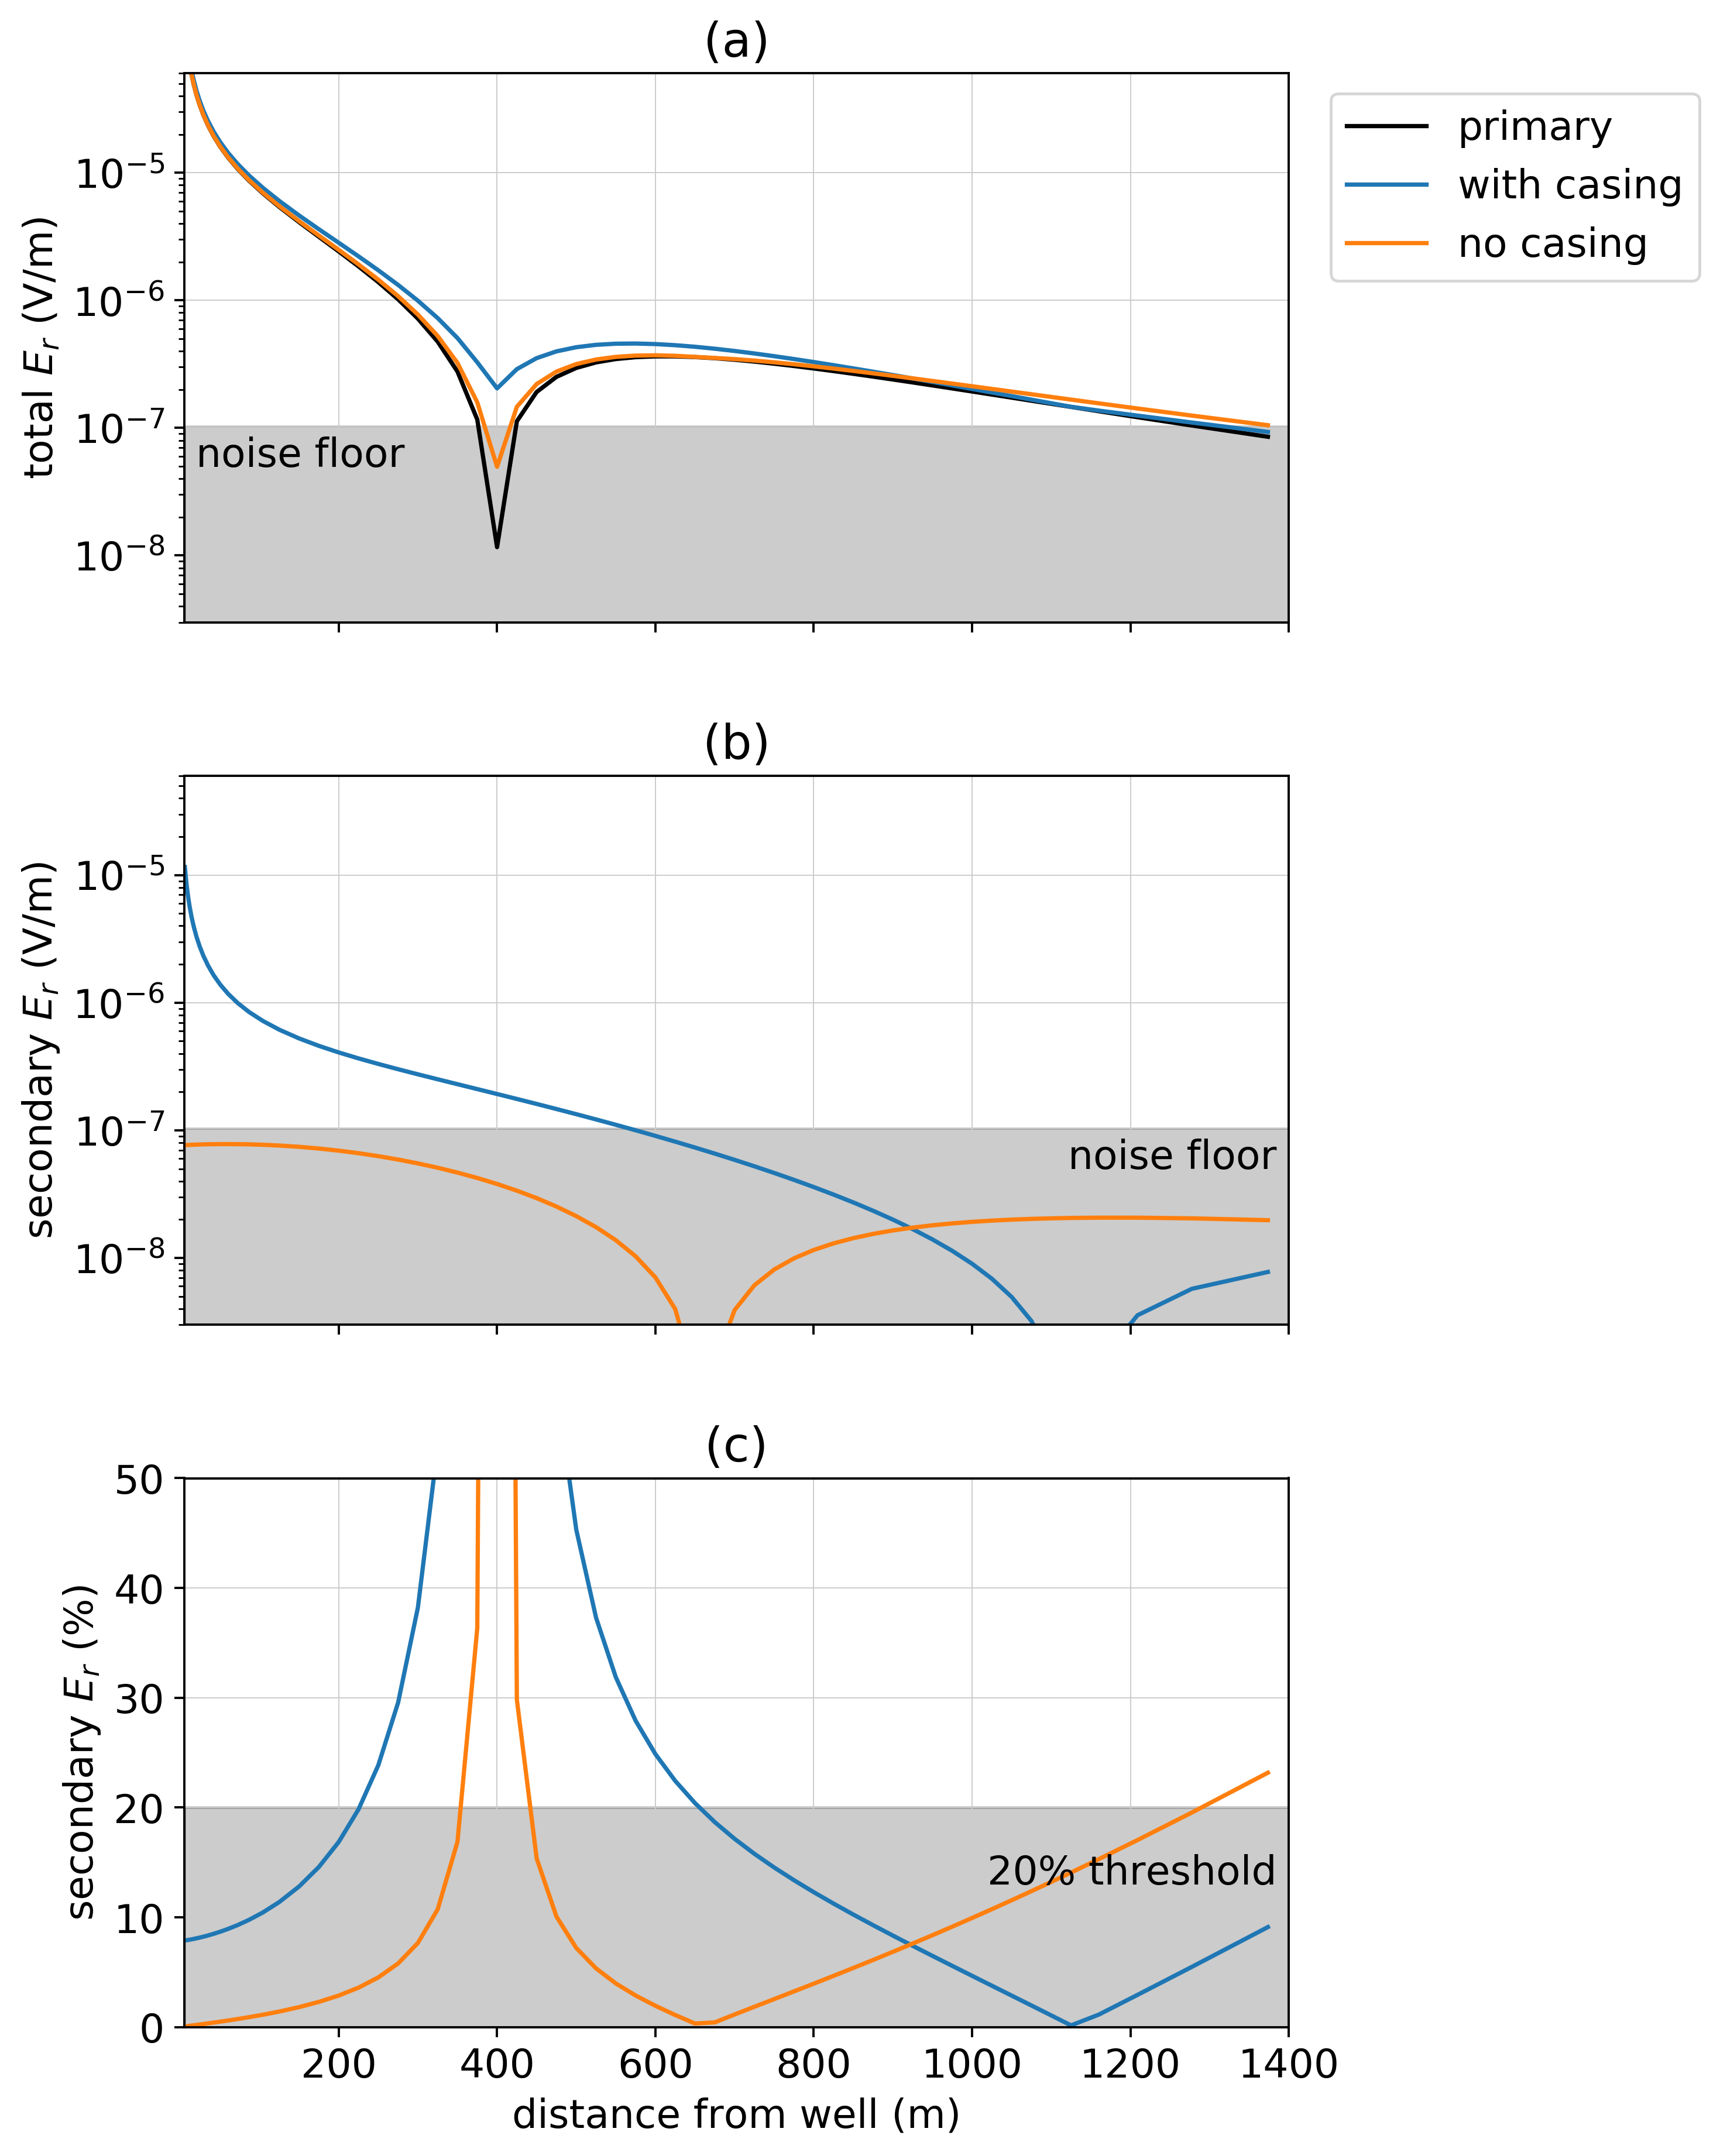
\includegraphics[width=0.8\textwidth]{figures/dc_casing/detectability_dipole.png}
    \end{center}
\caption{
    (a) Sum of the primary and secondary radial electric field due to a dipolar
    target with moment of 38 Am
    centered 50m from the well, either calculated with the
    casing (blue) or simply a dipole in a half-space (orange). (b) Secondary
    radial electric field due to a dipolar target in a halfspace with casing (blue) and without casing (orange).
    Secondary radial electric field as a percentage of the primary.
    The target is along a line $90^\circ$ from the
    source electrodes; this is the same line along which we measure data at the surface.
}
\label{fig:detectability_dipole}
\end{figure}


\subsubsection{Summary}
The examples presented here showed that conductive targets are much easier to excite than resistive targets. For deep targets, a downhole electrode is preferable to a top-casing source as it delivers more current at depth to excite the target and reduces the strength of the primary at the surface; this makes the secondary field a larger percentage of the primary. For targets in close proximity to the well, if the target is in contact with the well, that electrical connection enhances the response. Additionally, I showed that beyond helping excite a target, as was demonstrated by \cite{Schenkel1994}, the casing also improves detectability of secondary signals at the surface.

Designing a survey for a specific setting may require incorporation of 3D geologic structures and may include inversions to examine a survey's ability to recover a target. In this case, it is desirable to have a coarse-scale representation of the steel-cased well on the simulation mesh. This is the topic of the next section.

\section{Coarse-scale approximations of the well}
\label{sec:approximating_wells}

When approaching the inverse problem, many forward simulations are required, and typically, a 3D cartesian mesh, with cells that vary on the length scales of the geology, is desired. Thus, rather than performing a fine-scale simulation of the steel-cased well, we may wish to represent the well on a coarse mesh. In the literature, two main approaches arise: the first approximates the well as some form of ``equivalent source,'' such as a charge distribution (e.g. \cite{Weiss2016}); the second approach represents the well as a conductivity feature on the coarse-mesh (e.g. \cite{Swidinsky2013, Um2015, Yang2016, Kohnke2017, Puzyrev2017}, among others). Here, I will focus on the second approach, noting that a charge distribution along the length of the well can be computed with the 2D or 3D cylindrical code described in Chapter \ref{ch:casing-software}. Within the literature, there is disagreement among approaches for selecting the conductivity of the coarse-scale feature approximating the well. \cite{Um2015} replaces the fluid-filled cylinder with a solid rod having the same conductivity as the casing, arguing that it is the contrast between the conductivity of the well and the conductivity of the surrounding geology that is the most important factor; \cite{Puzyrev2017} also adopts this approach. Other authors have opted to preserve the cross-sectional conductance of the well \citep{Swidinsky2013, Kohnke2017}; this is consistent with the transmission-line model of the well discussed in \cite{Kaufman1990}. The aim of this section is to analyze these approaches.
\subsection{Replacing a hollow-cased well with a solid cylinder}
I consider a steel-cased well with a conductivity of $5\times10^6$ S/m that is embedded in a 0.1 S/m halfspace; the conductivity of the material that fills the well is the same as the background. The well has an outer diameter of 10 cm and a thickness of 1 cm, and I will vary its length. I will perform a top-casing experiment, where the positive electrode is connected to the casing at the surface. The return electrode is positioned 8 km away, and a cylindrically symmetric mesh is used in the simulations. I examine approximations that treat the casing as a solid cylinder with the same outer-diameter as the true, hollow-cased well.

The distribution of charges, or equivalently, the current in the casing, is the source of the electric response of the casing. Thus to judge if two models of the casing are ``equivalent'', I examine the current and charges as a function of depth. In Figure \ref{fig:approximating_wells_currents_charges}, I have plotted the vertical current and charges along the casing for the true, hollow cased well (solid), solid cylinder with conductivity equal to that of the casing, $5 \times 10^6$ S/m (dashed), and solid cylinder with a conductivity that preserves the product of the conductivity and the cross-sectional area of the conductor, $1.8 \times 10^6$ (dotted), for four different casing lengths, each indicated by a different color. Figure \ref{fig:approximating_wells_currents_charges} shows: (a) the vertical current along the casing, (b) the difference in current between the approximate model and the true model, (c) that difference as a percentage of the true solution (d) the charge per unit length, (e) difference in charge per unit length and (f) difference in charge per unit length as a percentage of the true solution.


\begin{figure}
    \begin{center}
    \includegraphics[width=\textwidth]{figures/dc_casing/approximating_wells_currents_charges.png}
    \end{center}
\caption{
    Currents (top row) and charges (bottom row) along the length of
    a hollow steel-cased well (solid lines), solid cylinder with
    conductivity equal to that of the steel-cased well (dashed-lines),
    and a solid cylinder with a conductivity such that the product of the
    conductivity and the cross sectional area of the cylinder is equal to that
    of the hollow-pipe (dotted lines). Each of the line-colors corresponds to a
    different casing length, as indicated in the legend.
    In (a), we show the vertical current in the casing,
    (b) shows the difference from the true, hollow-cased well
    in the vertical current within the casing, and (c) shows that difference as a percentage
    of the true currents. In (d), we show the charge per unit length along the casing, (e)
    shows the difference from the true, hollow-cased well and (e) shows that differences as
    a percentage of the true charge distribution.
    The x-axis on all plots is depth normalized by the length of the casing.
}
\label{fig:approximating_wells_currents_charges}
\end{figure}


For short wells, we see that the current decays linearly and that the charge distribution is nearly uniform above the end of the well, while for longer wells, the decay of the current is exponential in nature, as is the charge distribution. This behavior is consistent with that predicted by the transmission line solution described in \cite{Kaufman1993}. \cite{Kaufman1993} showed that the transition between the linear decay of currents and the exponential decay of currents is controlled by three factors: the cross sectional conductance of the well, the resistivity of the surrounding formation, and the length of the well. \cite{Schenkel1991} similarly summarized this behavior in the definition of the conduction length (equation \ref{eq:conduction_length}), which is the length over which the currents in the casing have decayed by a factor of $1/e$. For sufficiently conductive and short wells (e.g. $L_c / \delta \ll 1$, where $L_c$ is the length of the casing), the current decay is linear and independent of the conductivity, whereas for longer wells, ($L_c / \delta \gg 1$), the rate of decay of the currents is controlled by the conduction length (see equations 45 and 53 in \cite{Kaufman1993}).

In preserving the cross-sectional conductance, we see that the difference in currents and charges along the length of the well is negligible;  the maximum difference in currents for the 2000 m long well which has equivalent cross-sectional conductance is $7\times10^{-7}$ A as compared to the difference of 0.18 A when using the conductivity of the casing. This difference is important as it changes how much current is available to excite a target at depth. For a 2000 m long well, the current is overestimated by $> 150\%$ if the well is replaced by a solid cylinder with the same conductivity of the steel-cased well. It also changes the distribution of charges and thus the electric field due to the well. Figure \ref{fig:approximating_wells_currents_charges}e shows us that the extra conductance introduced when approximating the well using the conductivity equal to the casing results in a secondary dipolar charge on the casing. This in turn reduces the electric field we observe at the surface, as shown in Figure \ref{fig:approximating_wells_electric_fields}. For a long well, the difference can be as large as 40\% near the well.

\begin{figure}
    \begin{center}
    \includegraphics[width=\textwidth]{figures/dc_casing/approximating_wells_electric_fields.png}
    \end{center}
\caption{
    Radial electric field measured at the surface for a model of
    a hollow steel-cased well (solid lines), a solid cylinder with
    conductivity equal to that of the steel-cased well (dashed-lines),
    and a solid cylinder with a conductivity such that the product of the
    conductivity and the cross sectional area of the cylinder is equal to that
    of the hollow-pipe (dotted lines). Each of the line-colors corresponds to a
    different casing length, as indicated in the legend.
    In (a), we show the total radial electric field,
    (b) shows the difference in electric field from that due to the true, hollow-cased well,
    and (c) shows that difference as a percentage
    of the true electric fields.
    The x-axis on all plots is distance from the well normalized by the length of the casing.
}
\label{fig:approximating_wells_electric_fields}
\end{figure}


The numerical time-domain EM experiment used in \cite{Um2015} to justify the approximation of the well by a solid, conductive rod having the same conductivity as the steel-cased well used a 200 m long well with a thickness of 12.223 mm, outer diameter of 135 mm, conductivity of $10^{6}$ S/m in 0.033 S/m half-space. The conduction length of this well is 560 m; this is more than twice the length of the well. Therefore, the behavior of the currents falls into the linear regime, where the decay of currents is mostly independent of the conductivity, and thus the difference between using the conductivity of the casing or preserving cross-sectional conductance is less significant. However, if longer wells such as those typically employed in hydrocarbon settings, are considered, the behavior of the currents and charges depends upon the conductance of the casing, and thus that is the quantity that should be conserved in an approximation of the hollow-cased well by a solid rod.

In order to confirm that this conclusion is valid for variable geology, I have included a simulation with a 2 km long casing in a layered background. Each layer is 50 m thick and the conductivity was assigned randomly; three instances are included, as shown in Figure \ref{fig:random_layers}. The mean of the background conductivity is 0.1 S/m for each of the models.

\begin{figure}
    \begin{center}
    \includegraphics[width=\textwidth]{figures/dc_casing/random_layers.png}
    \end{center}
\caption{
    Three realizations of a 2km long casing in a layered background, where the conductivity of the
    layers is assigned randomly. Each layer is 50m thick, and the mean conductivity of the background
    is 0.1 S/m. The color of the title corresponds to the plots of the currents and charges in Figure
    \ref{fig:approximating_wells_currents_charges_random}
}
\label{fig:random_layers}
\end{figure}


The currents and charges along the length of the well for the true model, and a model approximating the well as a solid cylinder with equal cross-sectional conductance, are shown in Figure \ref{fig:approximating_wells_currents_charges_random}. For all of the models shown, the difference in both the casing currents and the charges are 5 orders of magnitude less than the amplitude of the total currents and charges; thus I conclude that approximating a hollow cylindrical steel casing by a solid cylinder with a conductivity that preserves cross-sectional conductance is valid for models with variable geology.

\begin{figure}
    \begin{center}
    \includegraphics[width=\textwidth]{figures/approximating_wells_currents_charges_random.png}
    \end{center}
\caption{
    (a) Total vertical current through the casing for the three layered-earth models shown in
    Figure \ref{fig:random_layers}. The solid lines indicate the response of the true, hollow steel cased-well
    and the dotted lines indicate the response of a solid cylinder having the same cross-sectional conductance
    as the hollow well. (b) Difference between the currents along the casing in the solid well approximation
    and the true, hollow well.
    (c) Charge per unit length for each of the models. (d) Difference in charge per unit length between the
    true model of the casing and the approximation which preserves cross-sectional conductance.
}
\label{fig:approximating_wells_currents_charges_random}
\end{figure}


\subsection{Cartesian grid}
\label{sec:approximating-cartesian}

In the previous section, I showed that a hollow, cylindrical steel-cased well can be approximated by a solid cylinder with equal cross-sectional conductance. In this section, I move to a coarser, cartesian mesh, such as might be employed when solving a 3D inverse problem. I examine a simple approximation of a steel cased well on a cartesian grid. I employ 4 tensor meshes, each with progressively larger cell widths for the finest cells that capture the casing. On each of the cartesian meshes, I approximate the casing by preserving the product of the conductivity and the cross sectional area on the mesh. For comparison, I run a fine-scale simulation on a 3D cylindrical mesh that accurately discretizes the casing; it uses 4 cells across the casing-wall. The casing model is similar to that used in previous examples: it is 1 km long, has an outer diameter of 10 cm, a thickness of 1 cm, and is embedded in a 0.1 S/m half-space. The positive electrode is connected to the top of the casing and a return electrode is positioned 1 km from the well-head.

The resultant currents and charge per unit length are shown in Figure \ref{fig:approximating_wells_cartesian}. In the top row, panel (a) shows the total current in a region approximating the well, along with the total current in the ``true'' cylindrical well (black line), (b) shows the difference between the current through the cartesian cells and the true model, and (c) shows the difference as a percentage. Similarly, in the bottom row, I show (d) the charge per unit length along the cylindrical well (black line) and cartesian-prism approximations, (e) the difference in charge per unit length from the charge per unit length on the true cylindrical model, and (f) that difference as a percentage of the charge per unit length on the cylindrical well.


\begin{figure}
    \begin{center}
    \includegraphics[width=\textwidth]{figures/approximating_wells_cartesian.png}
    \end{center}
\caption{
    Currents (top row) and charges (bottom row) along the length of
    a steel cased well represnted on a 3D cylindrical mesh which has
    4 cells radially across the width of the casing and 2.5m height (black line),
    a tensor mesh with 0.1m $\times$ 0.1m $\times$ 2.5m cells discretizing the casing (blue lines),
    a tensor mesh with 1m $\times$ 1m $\times$ 2.5m cells discretizing the casing (orange lines),
    and a tensor mesh with 10m $\times$ 10m $\times$ 10m cells discretizing the casing.
    The solid lines show simulations with an isotropic conductivity defined to preserve the
    product of the conductivity and cross-sectional area of the casing. The dashed lines
    use an anisotropic conductivity to represent the casing. The vertical component preserved the product
    of the conductivity and cross-sectional area of the casing while the horizontal components are an
    average of the resistivity and cross-sectional area of the casing and background
    (and equals the conductivity of the background, $0.1$ S/m, for both the 1m and 10m cells).
    In (a), we show the vertical current in the casing,
    (b) shows the difference from the true, hollow-cased well
    in the vertical current within the casing, and (c) shows that difference as a percentage
    of the true currents. In (d), we show the charge per unit length along the casing, (e)
    shows the difference from the true, hollow-cased well and (e) shows that differences as
    a percentage of the true charge distribution.
}
\label{fig:approximating_wells_cartesian}
\end{figure}


The approximation of the cylindrical well by a rectangular prism with width equal to the diameter of the casing introduces minimal error in the currents and charges computed using a finite volume approach, even though the casing is only captured by one cell across its width. Comparing the current along the length of the well for the 3D cylindrical well and the cartesian simulation with 0.1 m cells, we see that the error introduced is $< 2.5\%$ (until the end of the well where the current approaches zero). Similarly, the difference in the charge per unit length is $< \pm 1.25\%$. As successively coarser discretizations are used, accuracy is gradually lost; by doubling the cell sizes to 0.2 m, the error in the currents is $6\%$ at its maximum and $< \pm 3\%$ in the charge along the casing. A factor of 8 increase in cell size (0.8 m cells) results in a maximum error of $15\%$ in the currents. It is important to note that the forward simulation is conducted using a finite volume approach; other approaches such as finite difference or integral equation approaches may have worse agreement if care is not taken to handle large physical property contrasts, captured by a single cell, in the simulation.
Note that the behavior of the errors depends upon the properties of the casing (e.g. conductivity and length) as well as the conductivity of the background. This might be expected from the description of the casing conduction length (equation \ref{eq:conduction_length}). If the conduction length is large relative to the length of the well, the currents decay linearly, and the geometry and conductivity of the well are less significant in the behavior of the currents. Alternatively, if the conduction length is comparable to the length of the well, the currents decay exponentially with a decay rate that depends on the geometry and conductivity of the well. For example, if the background is more resistive, increasing the contrast between the casing and background, the errors are reduced. Using a background conductivity of $100 \Omega m$, the maximum error introduced in the current is $< 1\%$ with 0.1 m cells and $< 2\%$ with 0.8 m cells.

Depending on the level of accuracy required in a 3D simulation, there are several strategies that one might take to reduce this error. In some cases, local refinement can be achieved with a tetrahedral mesh, as is often employed when using finite element techniques (e.g. \cite{Weiss2016}), or an OcTree mesh \citep{Haber2007}. Other, more advanced approaches including upscaling and multiscale could also be considered. In an upscaling approach, one inverts for a conductivity model, which might be anisotropic, that replicates the physical behavior of interest \citep{Caudillo-Mata2017}. Multiscale techniques translate conductivity information from a fine-scale mesh to a coarse-scale mesh, on which the full simulation is to be solved, using a coarse-to-fine interpolation that is found by solving Maxwell's equations on the fine mesh locally for each coarse grid cell \citep{Haber2014, Caudillo-Mata2017a}. The 3D cylindrical forward simulation code described in Chapter \ref{ch:casing-software} and used in this example can serve a tool for validating and refining an approach to achieve the desired level of accuracy.

\section{Conclusion}
The work in this chapter is motivated by the increasing use of steel cased wells in geoscience problems, including monitoring applications such as carbon capture and storage and hydraulic fracturing. For geophysical imaging of targets at depth, the wells are beneficial as they can be used to channel currents to depth and enhance signals at the surface for targets that otherwise would be undetectable from a surface-based survey. Additionally, there is interest in considering the casing itself as the geophysical target in casing integrity experiments; here the aim is to detect flaws or breaks in the casing. These applications, coupled with advances in modeling capabilities, open up the potential for advancing the utility of electrical and electromagnetic imaging in settings with metallic-cased wells.

Despite this potential, the reality is that electric fields, especially if measured at the Earth's surface, are small. Secondary fields might only be a few percent of the primary field, and thus too insignificant to reliably detect the target of interest. The success of using a DC or EM survey then depends upon many details that pertain to understanding the basic physics, the effects of parameters of the casing, the background conductivity, location of the current electrodes, and discerning which fields should be measured. DC resistivity is the starting point, as it allows us to examine the currents, charges, and electric fields in the electrostatic limit, prior to introducing inductive effects and the influence of magnetic permeability in an EM signal, and as such, was the focus of this paper. Regarding the physics, a DC survey involves attaching a current generator to a conductive medium. This establishes a steady state current; the signal to which we are sensitive is the electric field that arises from charges that accumulate at interfaces separating regions of different conductivity. For this reason, most of our results are first presented as currents and charges.

The large contrasts in physical properties and significant variation in length scales due to long, thin, cylindrical, steel-cased wells prompt a number of questions about how the EM fields behave. In many cases, the finer details about the physical responses has challenged my intuition. With respect to the casing integrity application there were basic questions: how does a flaw in the pipe affect the currents and electric fields measured at the surface? Does the extent of the flaw change our ability to detect it (e.g. if it has a vertical extent of several meters versus a vertical extent of centimeters)? What happens if the flaw only comprises a part of the well, leaving some connectedness in the casing? When considering a geophysical experiment for imaging a target: is there a significant difference in the currents at depth between scenarios where a source electrode is connected to the well-head at the surface and one where the source electrode is offset from the well by a few meters? The surface signals are small; are there preferential geometries for the source and receiver electrodes that maximize signal/noise? A major goal of the DC survey will be to excite and detect target bodies. For problems, such as CO$_2$ sequestration, enhanced oil recovery, or hydraulic fracturing, the target may or may not be in contact with the well; how significant is an electrical contact between a target and the well in the data we measure at the surface?

Looking towards solving inverse problems in settings with steel-cased wells, it is advantageous to reduce the computational cost of the forward simulation because an inversion requires many forward simulations. There are several approaches that can be taken to achieve this; one common approach is to approximate the finely-discretized well with an approximation on a coarse-scale mesh. Currently, there is disagreement within the literature as to how this should be done. Some authors have advocated that the conductivity contrast between the casing and the background should be preserved and thus replace a hollow steel-cased well with a solid rod that has a conductivity equal to that of the casing. Other authors have opted to preserve the product of the conductivity and cross-sectional area of the casing, following the conclusions of the transmission-line solution shown in \cite{Kaufman1990}. What is the correct conductivity needed for substitution?

Some of the above questions have been addressed in theoretical papers extending back a few decades but numerical verification was often limited or carried out with simplifying assumptions. Other questions require the ability to carry out numerical modeling in 2D or 3D environments -- these tools are just now becoming available. My goal with this chapter has been to examine the scientific questions above and to promote insight about the solution by plotting the currents, charges, and electric fields.


%% The following is a directive for TeXShop to indicate the main file
%%!TEX root = ../../thesis.tex

\chapter{Electromagnetics with steel cased wells}
\label{ch:casing-em}

\section{Introduction}
In the previous chapter, I focussed on the physics of direct current (DC) resistivity experiments in settings with steel cased wells. This provided a fundamental understanding in terms of the charges, currents and electric fields. In this chapter, I shift attention to the electromagnetic (EM) problem where the fields and fluxes vary in time. EM can be advantageous in that for a given survey geometry, the response can be sampled at multiple frequencies or times, providing richer information than is available by only the electrostatic response in a DC experiment. The richness in information comes both from the additional physics introduced as inductive processes become relevant, as well as potentially multiple excitation directions as the formation currents change through time.

In addition to time-variation of fields and fluxes in an EM experiment, the physics in settings with steel casing is further complicated by the significant magnetic permeability of the steel. Typically, magnetic permeability is often neglected in EM simulations and inversions as the variations in permeability are typically much less significant than the role of conductivity in the data. However, steel has a permeability of $\geq 100$ $\mu_0$ \citep{wuhabashy1994}.

The role of permeable casings has been explored for inductive sources and receivers, primarily in the context of cross-well EM surveys \citep{Augustin1989, wuhabashy1994, Wilt1996, Becker1997, Lee1998, Lee2005, Kim2006}. For grounded sources, the influence of permeability is much less explored. More recently, some authors have included magnetic permeability in simulations with casings, (e.g. \citep{Kong2009}), but most of the published EM simulations of metallic cased wells neglect to include magnetic permeability (e.g. \citep{Swidinsky2013, Commer2015, Um2015, Fang2017, Puzyrev2017}). Within the publications that include permeability in grounded-source simulations, there is minimal analysis on how permeability alters the behavior of the currents in the earth or how it affects data measured at the surface. A notable exception is the work in \cite{Wait1985, Williams1985}. They developed an analytical model for a dipole-dipole frequency domain electromagnetic experiment over a halfspace with a conductive, permeable, and polarizable casing. Their simulations showed that if the casing is permeable, the apparent resistivity and phase measurements made at the surface data can be biased upwards as compared to only a conductive casing. Expanding on our understanding of how the permeability impacts the subsurface currents and the resultant measured data in a grounded-source experiment with a steel cased well is a prime goal of this chapter.

For numerical modelling, particularly when considering the inverse problem, it is advantageous to reduce the size of the mesh to reduce the computational cost. In Chapter \ref{ch:casing-dc}, I showed that for a DC resistivity experiment, preserving the product of the conductivity and the cross-sectional area of the casing is a viable strategy if the cells which encapsulate the casing are approximately equal in size to the diameter of the casing. It is questionable if this same approximation holds for EM experiments. Furthermore, it is unclear how to approximate the magnetic permeability on a coarse scale. \cite{Schwarzbach2018} suggests an upscaling strategy based upon that presented in \cite{Caudillo-Mata2017}, where one inverts for the conductivity and the permeability of the casing. By analyzing the the behavior of the fields and fluxes, we may be able to calibrate our expectations of upscaling strategies for permeability.

We have the choice to focus our analysis in the time-domain or the frequency-domain. Here, I choose to conduct the analysis in the time-domain. The physics of EM are arguably more intuitive in the time-domain, as all fields are real and we can step through changes with time. The frequency-domain requires that we consider the partitioning of electromagnetic energy into real and quadrature components; this additional step can be a hurdle to building intuition.

The chapter is organized as follows. In section \ref{sec:TDEM-casing}, I consider the time-domain EM (TDEM) response of a conductive well in a ``top-casing'' experiment where one electrode is connected to the top of the well and a return electrode is positioned some distance away on the surface. I examine the currents within the casing and in the surrounding geologic formation through time; this provides the foundation for understanding the EM casing response. Following from this, I introduce magnetic permeability in Section \ref{sec:permeable-casing} and demonstrate how it alters the current and the impact this has on data collected at the surface. Finally, in section \ref{sec:approximating-em}, I examine the the problem of approximating a conductive, permeable, steel-cased well and discuss some of the challenges that are unique to EM as compared to DC.

Source code for all of the examples shown in this chapter are available as Jupyter notebooks as outlined in Appendix \ref{app:code_list}.


\section{EM response of a conductive casing}
\label{sec:TDEM-casing}

As a starting point for this discussion, I first perform a simple numerical experiment to demonstrate the behavior of the currents in a time-domain EM experiment over a half-space. For this simulation, a positive electrode is positioned at the origin (where the casing will be)  and a return electrode is positioned 1km away (at x=1000 m). The conductivity of the background is $10^{-2}$ S/m, and the conductivity of the air is set to $1 \times 10^{-4}$ S/m. When we come to simulations with the casing, I have observed that contrasts near or larger than $\sim 10^{12}$ S/m leads to erroneous numerical solutions, and thus it is preferable to set the air to be more conductive than what it typically employed in EM simulations (often $\sim 10^{-8}$ S/m). A step-off waveform is used and the currents within the formation are plotted through time in Figure \ref{fig:tdem-background-total-currents}. Panel (a) shows a vertical cross section along the line of the wire, (b) shows a horizontal depth slice at 50 m depth and (c) shows a depth slice at 800 m depth. The images in panels (a), (b) and (c) are on the same color scale.


\begin{figure}
    \begin{center}
    \includegraphics[width=0.85\textwidth]{figures/em_casing/tdem-background-total-currents.png}
    \end{center}
\caption{
    Current density for a time domain experiment over a $10^{-2}$ S/m half-space.
    The positive electrode is on the surface where the well-head will be and the return electrode is at x=1000m. Each row corresponds to different time, as indicated in the plots in panel (c). Panel (a) shows a cross section through the half-space along the same line as the source-wire. Panels (c) and (d) show depth-slices of the currents at 54m and 801m depth.
}
\label{fig:tdem-background-total-currents}
\end{figure}





At time $t=0s$, the currents behave according to the DC solution. In panel (a), we see the flow of current from the source electrode, through the formation to the return electrode. Immediately after the source-current is shut-off, an image current develops in the formation; this image current acts to preserve the magnetic flux initially set-up by the source current. The image current flows in the same direction as the original current in the wire. This is opposite to currents in the formation, causing a circulation of current. The center of this circulation is visible as the null at x=500m (the mid-way point between the two current electrodes) which propagates downwards through time. Similarly, in the depth slices, we can see the image currents diffusing downwards and outwards with time. For example, between 1ms and 5ms, the image current passes 800m depth.

Having established the background response, I now consider a model with a steel-cased well. The well has a conductivity of $5 \times 10^6$ S/m and is 1km long; it has an outer diameter of 10cm and a 1cm thick casing wall. The mud which infills the well has the same conductivity as the background, $10^{-2}$ S/m. At this point, I focus on electrical conductivity only and set the permeability of the well to $\mu_0$. I will introduce variable magnetic permeability in the following section. The source electrode is connected to the top of the casing, and the return electrode is in the same position as the previous example (x=1000m). The same step-off experiment is run and the currents plotted in Figure \ref{fig:tdem-casing-total-currents}. I have added a fourth panel (a) which zooms in to the wellbore. Panels (b), (c) and (d) again show a cross-section of the currents in the formation and depth slices at 50m and 800m depth, respectively.


\begin{figure}
    \begin{center}
    \includegraphics[width=0.95\textwidth]{figures/em_casing/tdem-casing-total-currents.png}
    \end{center}
\caption{
    Current density for a top-casing time domain EM experiment with a conductive well ($5\times 10^6$ S/m).
    (a) Cross section in the immediate vicinity of the well.
    (b) Cross section through the formation.
    (c -- d) depth-slices.
}
\label{fig:tdem-casing-total-currents}
\end{figure}





At time, $t=0s$, we can see the increased current density along the length of the well, which correspondingly increases the current density deep within the formation. At the DC initial condition, currents flow away from the well, and eventually curve back to the return electrode. As in the previous example, an image current develops in the formation immediately after shut-off, which can be seen in Figure \ref{fig:tdem-casing-total-currents} (b). There is again a circulation of current, however the geometry of this circulation and the corresponding null is more complex than in the previous example. In Figure \ref{fig:tdem-casing-total-currents} (a), we see the background circulating currents being channeled into the well and propagating downwards. The depth range over which currents enter the casing depends upon time. At t=0.01 ms, the zero crossing, which distinguishes the depth between incoming and outgoing current in the casing, occurs at z=90 m, at t=0.1 ms it is at 225 m and by t=1 ms, the zero crossing approaches the midway point in the casing and is at 470 m depth. At later times, the downward propagation of this zero-crossing slows as the image currents are channeled into the highly conductive casing.

Further out in the formation, we similarly see the interaction of the diffusing formation currents set up at DC and the image currents. Rather than being centered at the midway point between the positive and negative electrodes as in the half-space example (Figure \ref{fig:tdem-background-total-currents}), the center of the circulating currents shifts with time. At early times, it is closer to the well, while at later times, it is closer to the mid-way point. By 10ms, the impact of the well is much less evident and the currents are very similar in character to those obtained in the half-space experiment.

On the side of the well opposite to the wire, we also see a null develop; it is visible in the cross sections in panel (a). To help understand this, we examine the depth slices in panel (c). Behind the well, we see that as the image currents diffuse downwards and outwards, some of those currents are channeled back towards the well; this is visible in the depth slice at $10^{-4} s$. These channeled currents are opposite in direction to those the formation currents set up at t=0, which also are diffusing downwards and outwards; where these two processes intersect, there is a current shadow.

We can isolate the ``casing response'' by taking the difference between the currents generated when the casing is present (Figure \ref{fig:tdem-casing-total-currents}) and those generated in the half-space model (Figure \ref{fig:tdem-background-total-currents}). This is plotted in Figure \ref{fig:tdem-casing-secondary-currents}. Within the casing and the surrounding formation, these secondary currents are cylindrically symmetric. This might not be immediately intuitive given the complexity of the behavior observed in Figure \ref{fig:tdem-casing-total-currents}, however, it is a highly conductive, cylindrically symmetric target, and the main impact it has on the physical behavior is that it channels currents along its length. At all times, there is a downward-going secondary current within the casing. This results in dipolar-like currents within the surrounding formation.


\begin{figure}
    \begin{center}
    \includegraphics[width=0.95\textwidth]{figures/em_casing/tdem-casing-secondary-currents.png}
    \end{center}
\caption{
    Difference in current density for a time domain experiment which includes a conductive steel-cased well (as in Figure \ref{fig:tdem-casing-total-currents}) and an experiment over a halfspace (as in Figure \ref{fig:tdem-background-total-currents}).
}
\label{fig:tdem-casing-secondary-currents}
\end{figure}





\subsection{Data}

On the surface, we can measure electric field data and/or the time-rate of change of the magnetic field ($db/dt$) as a function of time. Due to the cylindrical symmetry of the currents in Figure \ref{fig:tdem-casing-secondary-currents}, we can expect that the radial electric field and the tangential $db/dt$ will be most impacted by the presence of the casing.

\subsubsection{Electric field}

In Figure \ref{fig:surface_e_fields_overview}, I show surface electric field data for 2 times, an early time (0.01 ms) and a later time (5 ms). The top row shows data from the background model. The two panels on the left show the electric field at the surface at (a) 0.01 ms and (b) 5 ms. On the right, (c) shows the radial electric field measured along the x=0m line (indicated by the white-dashed lines in (a) and (b)), and (d) shows a time-decay for a receiver positioned 300m from the well (indicated by the red dot in (a) and (b)). Data that are positive are plotted with the solid lines and data that are negative are plotted with dashed lines. The red dots in panel (c) correspond to the 300m offset location where the data in (d) are taken from. Similarly, the blue and green dots in (d) correspond to the time-channels shown in (c). The middle row shows the same information but for the simulation with the conductive well, and the bottom row shows the difference between the casing and background data (casing minus background).

\begin{figure}
    \begin{center}
    \includegraphics[width=\textwidth]{figures/em_casing/surface_e_fields_overview.png}
    \end{center}
\caption{
    Simulated electric field at the surface of the earth at (a) 0.01 ms and (b) 5 ms after shut-off for the halfspace model.
    (c) Radial electric field data measured along the survey line shown in white in (a) and (b) at 0.01 ms (blue) and 5 ms (green).
    (d) Radial electric field as a function of time at 300 m along the survey line (shown in the red dot in (a)).
    The red dots in (c) correspond to the data observed at 300 m offset
    and the blue and green dots in (d) correspond to the 0.01 ms and 5 ms data.
    Similar information is shown in (e), (f), (g) and (h) for the model with the conductive casing.
    The difference in the radial electric field data (casing minus halfspace) is shown in (i), (j), (k) and (l).
    %The difference is also shown as a percentage of the halfspace solution at 0.01ms and 5ms in (m)
    %and through time at 300m offset in (n).
}
\label{fig:surface_e_fields_overview}
\end{figure}






At early times (0.01ms), the behavior of the geometry of the electric field is fairly complex (panel a). The electric field we observe results from a combination of the diffusing galvanic and image currents. The galvanic currents, set up at DC, are dipolar in nature, with field lines directed radially outward from the positive electrode located at x=0m. The image current is directed in the negative x-direction and causes some inward deflection of the fields (this can also be observed at 0.01ms in Figure \ref{fig:tdem-background-total-currents}). A sketch of both current systems is shown in Figure \ref{fig:current-systems-sketch}


\begin{figure}
    \begin{center}
    \includegraphics[width=0.75\textwidth]{figures/em_casing/current-systems-sketch.png}
    \end{center}
\caption{
    Sketch of the plan-view geometry of the early-time galvanic currents (left) and image currents (right) in a time-domain EM experiment over a half-space.
    Through time, both current systems diffuse downwards and outwards as they decay.
    The wire follows a straight line between the negative and positive electrodes. The green dashed line shows where we are measuring the
    radial electric field data. Prior to shut-off, current in the wire flows from
    the negative to the positive electrode. In the earth, the galvanic currents are dipolar in nature and flow
    from the positive to the negative electrode. Along the survey-line, the radial component of the galvanic currents always points outwards.
    Immediately after shut-off, image currents are induced in the earth. They are oriented in the same direction as the original current in the wire
    and are directed away from the negative electrode towards the positive. Along the survey-line, the radial component of the image currents is always pointed inwards.
}
\label{fig:current-systems-sketch}
\end{figure}





The radial electric field data at offsets less than 300m are primarily influenced by the geometry of the image currents, while beyond 300m, the data are primarily influenced by the dipolar galvanic currents. Diffusion of both current systems continues through time. By 5 ms the image current has passed and the geometry of the fields reflects that of the diffusing galvanic currents. This means that the electric fields are a diffuse dipolar shape that is centered at the midpoint of the wire (e.g. as in Figure \ref{fig:tdem-background-total-currents}b at 1 and 5 ms). Along our survey line, the electric field is oriented mainly in the negative y-direction, but with a slight outward deflection due to the dipolar nature of the fields, and are therefore positive. Through time, we can similarly see the impact of the passing image current. At very early times, the data are positive, as the galvanic currents and associate electric field are the main contributor to the response. When the image current arrives, just past $0.01$ ms, the electric field is deflected inwards, reversing the sign of the radial electric field data. The second sign-reversal occurs at $\sim$ 0.3ms; at this point, the image current has diffused considerably, and we again return to a geometry that is mainly influenced by the diffusing galvanic currents.

I now consider the data when a casing is present. The casing introduces further complexity as it channels both galvanic and image currents. We can see the impact in the geometry of the fields in (e). The channeled currents are directed inwards, towards the well, giving the large negative radial electric field response observed at short offsets in (g). In panel (g), we see that this additional current-channeling pushes the sign reversal that we observed in the early time in (c) for the background model to a further offset. At later times, we continue to see the impact of the casing as the diffusing currents are deflected inwards (panel f). The result is that the radial electric field data remain negative through time as can be seen in (g) and (h).

The story simplifies if we examine the difference between the data from the model with the casing and those simulated with the background. Essentially, by subtracting the background data from the casing data, we remove the 3D survey geometry from the behavior of the fields, and are left with the current-channeling behavior. The well is a highly conductive feature and once the source current is shut off, the diffusing image current and galvanic currents are channeled towards it. The result is the cylindrically symmetric fields shown in (g) and (h). The electric field is directed radially inwards, and thus the secondary ``casing-response'' in (k) and (l) is always negative through time.

\subsubsection{Time rate-of-change of the magnetic flux}

We can examine the $db/dt$ data at the surface. Figure \ref{fig:surface_dbdt_overview}, shows the $db/dt$ data for the background (top row), casing model (second row), and difference between them (third row). Additionally, I include plots of the $db/dt$ data difference as a percentage of the background response in (m) and (n). The data plotted in the rightmost column (plots (c), (d) and below) are the azimuthal component of $db/dt$ along the white-dashed lines shown in panels (a) and (b).



\begin{figure}
    \begin{center}
    \includegraphics[width=\textwidth]{figures/em_casing/surface_dbdt_overview.png}
    \end{center}
\caption{
    Simulated $db/dt$ at (a) 0.01 ms and (b) 5 ms after shut-off for the halfspace model.
    (c) Tangential $db/dt$ measured along the white line in (a) and (b) at 0.01 ms (blue) and 5 ms (green).
    (d) Tangential $db/dt$ as a function of time at 300 m along the survey line (shown in the red dot in (a)).
    Similar information is shown in (e), (f), (g) and (h) for the model with the conductive casing.
    The difference in the $db/dt$ data (casing minus halfspace) is shown in (i), (j), (k) and (l).
    The difference is also shown as a percentage of the halfspace solution at 0.01 ms and 5 ms in (m)
    and through time at 300 m offset in (n).
}
\label{fig:surface_dbdt_overview}
\end{figure}





The $db/dt$ response is quite 3-dimensional in its geometry. At early times (panel (a), 0.01 ms), we have a rotational component that arises from the downward-directed current density at the positive electrode, located at the origin. We also have a contribution from the horizontal image-currents and galvanic currents, which complicates the behavior between x=0 and x=1000m. Near the surface, there is a y-directed component from these current systems. Later in time (5 ms) the $db/dt$ data in (b) are primarily influenced by the diffusing horizontal currents and thus $db/dt$ is oriented in the y-direction along the wirepath. The difference between the data from the simulation with the casing and without is much less dramatic than we observed in the electric field data. It is really only the late times at short offsets that are significantly impacted; beyond 400m offset from the well, the difference between the $db/dt$ data with the casing (f) and without (c) is less than 10\% for the 1ms data. In contrast, the electric field data in Figure \ref{fig:surface_e_fields_overview} differed by several orders of magnitude different at all offsets shown.

To summarize the above results, we see that each data-type is sensitive to different aspects of the physics. The radial electric field data are influenced by radial currents, which, as seen in the Figure \ref{fig:tdem-casing-secondary-currents}, are significantly altered near the surface over a large range of offsets when the casing is present. The tangential $db/dt$ data, however, are primarily influenced by vertical currents, which are most altered near the wellbore.


\subsection{Discussion}
There are a number of points to highlight in these examples. The first, which has been noted by several authors (e.g. \cite{Schenkel1994, Hoversten2015}), is that the casing helps increase sensitivity to targets at depth. This occurs by two mechanisms: (1) at DC, prior to shut-off, the casing acts as an ``extended electrode'' leaking current into the formation along its length; (2) after shut-off, it channels the image currents and increases the current density within the vicinity of the casing. The second point to note is that there are several survey design considerations raised by examining the currents: targets that are positioned where there is significant current will be most illuminated. If the target is near the surface and offset from the well, a survey where the source wire runs along the same line as the target will have the added benefits of the excitation due to the image currents. These benefits are twofold: (1) the passing image-current increases the current density for a period of time, and (2) the changing amplitude and direction of the currents with time generate different excitations of the target. This should provide enhanced information in an inversion, as compared to a single excitation that is available from a DC survey. For deeper targets in this experiment, the passing image current has diffused significantly, and thus it appears that the wire location has less impact on the magnitude of the current density with location. However, it is possible that increasing the wire-length could be beneficial. This extension is straightforward and could be examined with the provided script. Often, little attention is paid to the wirepath in an EM survey, and only the electrode positions are considered as a part of the survey design. These examples show that the image currents, whose geometry is dictated by the geometry of the wirepath, have a significant influence on the behavior of the currents and the resultant data. Thus, these examples also provide motivation for thinking of the wirepath as a component of the EM survey design.


\section{EM response of permeable casings}
\label{sec:permeable-casing}

The previous section demonstrated the behavior of the currents in a TDEM experiment with a conductive casing; in this section, I am interested in building an understanding of how the magnetic permeability of the pipe affects the currents the EM response. Using the same survey setup and casing geometry as in Figure \ref{fig:tdem-casing-total-currents}, I now include magnetic permeability in the simulation. The  permeability of the casing is set to $\mu = 100\mu_0$ and the resultant currents are shown in Figure \ref{fig:tdem-permeable-total-currents}.


\begin{figure}
    \begin{center}
    \includegraphics[width=0.95\textwidth]{figures/em_casing/tdem-permeable-total-currents.png}
    \end{center}
\caption{
    Current density for a top-casing time domain EM experiment over a $10^{-2}$ S/m half-space and a 1km-long, conductive, permeable steel-cased well ($5 \times 10^{6}$ S/m, $100\mu_0$).
}
\label{fig:tdem-permeable-total-currents}
\end{figure}






The early-time behavior of the currents is very similar to what we observed in the case of a conductive well (Figure \ref{fig:tdem-permeable-total-currents}). As we move to later times, however, we can see that the permeability of the steel introduces further complexity into the behavior of the currents. Notably, in Figure \ref{fig:tdem-permeable-total-currents}(a) at 5ms and 10ms, there is a vertical circulation of currents within the well-casing; near the inner wall of the casing, the currents are moving downwards, while near the outer wall, the currents are moving upwards. This is particularly noticeable near 750m depth in the 5ms image. The behavior of the currents within the formation is also more complex. By 10ms, the impact of the conductive casing was minimal on the behavior of the formation currents, whereas here, we see that the permeable and conductive casing still significantly alters the formation currents (as compared to Figure \ref{fig:tdem-background-total-currents}b).

To isolate the influence of magnetic permeability, I take the difference between the currents observed in the example with the conductive, permeable well (Figure \ref{fig:tdem-permeable-total-currents}) and those observed in the conductive well (Figure \ref{fig:tdem-casing-total-currents}). The result is shown in Figure \ref{fig:tdem-permeable-secondary-currents}.


\begin{figure}
    \begin{center}
    \includegraphics[width=0.95\textwidth]{figures/em_casing/tdem-permeable-secondary-currents.png}
    \end{center}
\caption{
    Difference in current density for a time domain experiment which includes a conductive, permeable steel-cased well (as in Figure \ref{fig:tdem-permeable-total-currents}) and an experiment over a conductive well (as in Figure \ref{fig:tdem-casing-total-currents}).
}
\label{fig:tdem-permeable-secondary-currents}
\end{figure}





At the DC limit, magnetic permeability has no influence on the behavior of the currents. However, as we move to later times, EM effects become relevant and we begin to see the impact that permeability has on the behavior of the currents. The generation of poloidal currents within the casing wall is not an effect that can be caused by conductivity alone.  Often in EM problems the magnetic field, $\vec{h}$ and the magnetic flux density $\vec{b}$ are treated interchangeably, which is sensible when $\mu = \mu_0$ everywhere in the domain. However, when variable permeability is introduced, the distinction is important. Figure \ref{fig:casing-mu-sketch} demonstrates how the vertical circulation of current can arise due to the interplay between the currents and corresponding rotational magnetic fields and fluxes. The downward directed current density within the casing (a) generates a toroidal magnetic field everywhere in space (b) according to Ampere’s law. The magnetic flux is related to the magnetic field through the constitutive relation, and since the pipe is much more permeable than the background, the magnetic flux density is concentrated within the pipe. Once the transmitter is shut-off, the magnetic flux decreases, and the time variation of the magnetic flux generates rotating electric fields (d) according to Faraday’s law. Finally, the electric field is related to the current density through Ohm’s law, and therefore the rotating current density is concentrated within the pipe (e). If the pipe is only conductive and not permeable, then there is no concentration of the magnetic flux, as in (c). Instead, the magnetic flux has identical geometry to the magnetic field, and by symmetry, the rotation of the electric field cancels, leaving only a vertical component.


\begin{figure}
    \begin{center}
    \includegraphics[width=\textwidth]{figures/em_casing/casing-mu-sketch.png}
    \end{center}
\caption{
    Sketch demonstrating how a vertical circulation of current can arise inside of a permeable casing in a top-casing TDEM experiment.
    A source current is applied and (a) currents flow downwards through the pipe. (b) Currents generate rotational magnetic fields according
    to Ampere's law. (c) Magnetic flux is concentrated in the permeable pipe according to the constitutive relation between $\vec{b}$ and $\vec{h}$.
    (d) The magnetic flux varies with time after shut-off, and the time-varying magnetic flux creates rotational electric fields according to Faraday's law.
    (e) Currents associated with those electric fields are concentrated in conductive regions of the model in accordance with Ohm's law.
}
\label{fig:casing-mu-sketch}
\end{figure}





\subsection{Data}

As in Figure \ref{fig:tdem-casing-secondary-currents}, the secondary currents due to the permeability of the well are cylindrically symmetric. In the data, we then expect that the radial electric field will be minimally impacted at early times, but at later times, we will see the influence of permeability. Figure  \ref{fig:surface_e_fields_permeable} shows the radial electric field data for the conductive casing (top row), and permeable casing (second row). As well as the difference (permeable minus conductive) and difference as a percentage of the data simulated with the conductive well in the third and fourth rows, respectively. At early times, the impact of permeability is minimal. For example, at 0.01 ms, it is only the data very near the wellbore (less than 100m offset) that are marginally impacted. At the later time-channel, however, the difference is significant. At 5 ms  the difference between including permeability and not is over 40\% for all offsets shown (panel m). Through time, at the 300 m offset, we can see that the response decays more slowly, particularly in the time window between 2 ms and 100 ms. The maximum difference is $> 4000 \%$ at 20 ms; in the conductive well-case (d), the response has decayed to $\sim 10^{-8}$ V/m, while in the permeable well (h), the value of the electric field is nearly two orders of magnitude larger.



\begin{figure}
    \begin{center}
    \includegraphics[width=\textwidth]{figures/em_casing/surface_e_fields_permeable.png}
    \end{center}
\caption{
    Simulated electric field at the surface of the earth, as was presented in \ref{fig:surface_e_fields_overview}.
    The top row (a -- d) are the data simulated with the conductive casing. The second rows (e -- h) are the data
    simulated with the conductive, permeable casing. The third row (i -- l) is the difference (permeable and conductive minus conductive only),
    and the fourth row (m and n) show the difference as a percentage of the conductive solution.
}
\label{fig:surface_e_fields_permeable}
\end{figure}





Although one might typically associate magnetic permeability with a large impact on the magnetic fields and fluxes, the difference in the $db_{\theta}/dt$ data is much less significant and localized to short-offsets, as can be seen in Figure \ref{fig:surface_dbdt_permeable}.



\begin{figure}
    \begin{center}
    \includegraphics[width=\textwidth]{figures/em_casing/surface_dbdt_permeable.png}
    \end{center}
\caption{
    Simulated $db/dt$ at the surface of the earth, as was presented in \ref{fig:surface_dbdt_overview}.
    The top row (a -- d) are the data simulated with the conductive casing. The second rows (e -- h) are the data
    simulated with the conductive, permeable casing. The third row (i -- l) is the difference (permeable and conductive minus conductive only),
    and the fourth row (m and n) show the difference as a percentage of the conductive solution.
}
\label{fig:surface_dbdt_permeable}
\end{figure}





\subsection{Down-hole source}
The impact of the magnetic permeability of the casing is much more significant if we consider an experiment in which one electrode is positioned within the borehole. In this case, the wire path is through the borehole, and the vertical current through it generates a azimuthal magnetic field that is essentially perfectly coupled to the permeable casing. I demonstrate this with an experiment where the positive electrode is attached to the permeable casing at 950m depth. The currents through time are shown in Figures \ref{fig:tdem-permeable-total-currents-downhole} and \ref{fig:tdem-permeable-secondary-currents-downhole} which show the total currents and the difference between an experiment with the permeable pipe and one with a conductive pipe whose permeability is $\mu_0$, respectively.

\begin{figure}
    \begin{center}
    \includegraphics[width=0.95\textwidth]{figures/em_casing/tdem-permeable-total-currents-downhole.png}
    \end{center}
\caption{
    Current density for a down-hole time domain experiment with a conductive, permeable steel-cased well ($5 \times 10^{6}$ S/m, $100\mu_0$).
    The positive electrode is connected to the casing at 950 m depth and the return electrode is on the surface at $x=1000$ m.
}
\label{fig:tdem-permeable-total-currents-downhole}
\end{figure}







\begin{figure}
    \begin{center}
    \includegraphics[width=0.95\textwidth]{figures/em_casing/tdem-permeable-secondary-currents-downhole.png}
    \end{center}
\caption{
    Difference in current density for a down-hole time domain experiment with a conductive,
    permeable steel-cased well (as in Figure \ref{fig:tdem-permeable-total-currents-downhole}) and a similar experiment with a conductive well.
}
\label{fig:tdem-permeable-secondary-currents-downhole}
\end{figure}





Shortly after shut-off, currents along the entire length of the pipe contribute to the difference in the response between the permeable pipe and a conductive pipe. This is reflected in the radial electric field data shown in Figure \ref{fig:surface_e_fields_permeable_downhole}

In the radial electric field data, shown in Figure \ref{fig:surface_e_fields_permeable_downhole}m, this corresponds to a difference of over 60\% at 1000m offset in the 5ms data.


\begin{figure}
    \begin{center}
    \includegraphics[width=\textwidth]{figures/em_casing/surface_e_fields_permeable_downhole.png}
    \end{center}
\caption{
    Simulated electric field at the surface of the earth, as was presented in \ref{fig:surface_e_fields_permeable}
    for a TDEM experiment in which the positive electrode is coupled to the casing at a depth of 950m.
}
\label{fig:surface_e_fields_permeable_downhole}
\end{figure}






\subsection{Discussion}
Magnetic permeability introduces yet another complication into the physics of EM in settings with steel-cased wells. In the top-casing experiment, we saw that by introducing permeability, a circulation of current in which current travelled downwards near the inner wall of the well-casing and upwards along the outer wall of the well casing, was generated. Such an effect is not observed if the casing is only conductive. This indicates that it is important to model both permeability and conductivity in numerical simulations to capture the physics; this is not commonly done in geophysical electromagnetic simulations. Furthermore, even low-frequency or late-time data, which are sometimes treated as DC, may be impacted by magnetic permeability. Typically one might associate magnetic permeability with most significantly impacting magnetic field data, however these results show that the electric field in a top-casing experiment can be off by $>$40\% at late times, even 1000m from the well if permeability is not considered in the simulation. On the positive side however, one  benefit that the permeability of the steel may have in time-domain EM imaging experiments is that it increases the current density within the formation at later times. As a result, there is a long time-window over which a target may be excited.
\section{Approximations to a steel cased well}
\label{sec:approximating-em}

The above simulations accurately discretize the casing, with 4 cells across the thickness of the casing wall. This is suitable for simulations in which the aim is to examine the physics. When considering an inversion, which requires many forward simulations and in which it is often preferable to use a cartesian grid to capture the geologic structures of interest, it may not be feasible to use such a highly-refined mesh to capture the finer details of the physics.

In the previous chapter, I showed that if we treat the well as a solid cylinder with a conductivity that preserves the product of the conductivity and cross-sectional area of the casing, we achieved an identical solution (within numerical error) at DC for the total current and charge-per-unit-length along the casing (see Section \ref{sec:approximating_wells}). This raises the question about whether, or not, this same approximation can be used for an electromagnetic experiment. Also, is there a straight-forward approximation that can be used to estimate the magnetic permeability for a coarse-scale representation of the well? In this section, I examine these two questions, first by considering a conductive well, and then introducing permeability.
\subsection{Electrical conductivity}
We consider the same model of a 1km long, conductive well ($5 \times 10^6$ S/m) in a $10^{-2}$ S/m half-space as used in Section \ref{sec:TDEM-casing} and perform a similar TDEM experiment in which one electrode is connected to the top of the casing and a return electrode is positioned 1km away. The approximate model I use is a solid cylinder which has a conductivity of $1.8 \times 10^6$ S/m, so that both the true and approximate models have equal cross-sectional conductances. Both simulations are performed on identical meshes; this minimizes numerical differences that might otherwise occur from employing different discretizations.

To compare the responses, I first consider the total current along the length of the well. If the approximation is correct, we should expect that the total current density in the hollow-cased well is equal to the total current density in the cylinder approximating the well through time. Figure \ref{fig:approx_casing_currents} shows (a) the current at two times (0.01ms and 5ms) along the length of the well, and (b) current at 500m depth through time for the true solution. Similarly, (c) and (d) show the current for the approximation to the well, (e) and (f) show the difference (approximation minus true), and (g) and (h) show that difference as a percentage of the true solution. At early times, there is good agreement between the two solutions; at 0.01ms, the percent-error in (g) is negligible and beyond 200m depth in (e), the error is 5 orders of magnitude smaller than the true current. Above 200m depth, we do see some coherent error that reaches a maximum of $\sim10^{-3}$ A near the surface. However, this is still several orders of magnitude smaller than the true current at 0.01ms. At later times the approximate solution underestimates the true current. At 5ms, the current is underestimated by 8\% along the entire length of the well, as can be seen in (g). Through time, the error shown in (h) reaches a maximum of nearly 10\% at 8ms. There is a large increase in percent difference beyond 30ms, this is simply because we are dividing the difference by the very small current at the late times.

\begin{figure}
    \begin{center}
    \includegraphics[width=\textwidth]{figures/em_casing/approx_casing_currents.png}
    \end{center}
\caption{
    (a) Downward-directed current (a) within the casing at 0.01ms (blue) and 5ms (green)
    and (b) as a function of time at 500m depth for the true, hollow-cased well.
    (c), (d) Current in the approximate model which treats the casing as a solid cylinder.
     The conductivity of the cylinder approximating the well is chosen so that both models have
    equal products of the conductivity and the cross sectional area.
    (e), (f) Difference between the current in the approximate model and the true model (approximate minus true).
    (g), (h) Difference as a percentage of the true solution.
}
\label{fig:approx_casing_currents}
\end{figure}





In electric field data measured at the surface, similar errors are observed. Figure \ref{fig:surface_e_fields_approx_casing} shows the electric field data for the true model (top row), approximate model (second row), difference between the approximate and true models (third row) and difference as a percentage (fourth row). At early times (0.01ms), there is minimal difference, but at 5ms, there is an 8\% difference between the data generated with the true model and those generated with the approximate model. At 300m offset, the time-period between 1 and 10 ms is when we observe the largest error (panel n).

Errors of 8-10\% is not as egregious as neglecting magnetic permeability, but the anomalies that we will be looking for when considering subsurface injections are small and may only comprise 10\% to 20\% of the background signal, so an error of 10\% is certainly not negligible.

\begin{figure}
    \begin{center}
    \includegraphics[width=\textwidth]{figures/em_casing/surface_e_fields_approx_casing.png}
    \end{center}
\caption{
    Simulated electric field at the surface of the earth, as was presented in \ref{fig:surface_e_fields_overview}.
    The top row (a -- d) are the data simulated with the true, conductive casing.
    The second rows (e -- h) are the data
    simulated with the solid cylinder approximating the well.
    The third row (i -- l) is the difference (approximate minus true),
    and the fourth row (m and n) show the difference as a percentage of the true solution.
}
\label{fig:surface_e_fields_approx_casing}
\end{figure}





In order to provide more context for where this approximation is breaking down, I have plotted the current density, charge density and electric fields through time in Figure \ref{fig:electric-casing}. Panel (a) shows the true current density, (b) shows the secondary current density (the difference between the simulation using the approximation of the casing and that using the true casing), (c) shows the true charge density (d) shows the secondary charge density, (e) shows the true electric field, and (f) shows the secondary electric field. Note that (a) and (b) are on the same logarithmic color scales as are (e) and (f). Panels (c) and (d) are each have their own associated linear colormap. Panels (b), (c) and (e) are effectively looking at ``what physics are we introducing by making by making this approximation?''

\begin{figure}
    \begin{center}
    \includegraphics[width=0.9\textwidth]{figures/em_casing/electric-casing.png}
    \end{center}
\caption{
    (a) True current density (b) difference between the currents in the simulation with the approximation to the conductive well and the true solution (secondary currents), (c) True charge density, (d) secondary charge density, (e) true electric field, (f) secondary electric field.
}
\label{fig:electric-casing}
\end{figure}





At the DC limit, the solutions are in agreement, with the exception that the current distribution between the true casing and the approximate casing are different inside of the well, as expected. There is also a small secondary electric field at the bottom of the pipe -- this is because by treating the pipe as a solid cylinder, we have introduced a conductivity contrast, and thus small secondary charge at that bottom interface. This however has minimal impact on the currents in the formation or data measured at the surface.

Shortly after shut-off, however, the approximation begins to break down. There is a dipolar charge introduced on the casing with a concentrated negative charge density near the top and a positive charge density beneath that. Corresponding to the positive charges, there are similarly outward-directed currents and electric fields. As time progresses, the secondary dipolar charge and associated currents and electric fields spreads out along the length of the well.

The passing image current changes the geometry of the currents and distribution of charges. At DC, the well has a positive charge along its length and all currents are outward from the well. The incoming image current is a source of the negative charges; the currents enter the conductive casing from the resistive background, thus negative charges build up at the interface. This indicates that the conductivity contrast between the background and the casing is important when considering EM effects. At DC, the approximation of the well by a cylinder with equal product of the conductivity and the cross sectional area is correct. Any alteration of the conductivity would introduce errors in the initial condition. However, the approximation does not hold through time as the geometry of the current-systems changes. This suggests that perhaps a conductivity which varies with time, and possibly along the length of the casing, may be necessary in order to accurately approximate the casing on a coarse scale.


\subsection{Magnetic permeability}
Clearly, if we do not have a suitable approach for estimating a coarse-scale  conductivity of a well in an EM experiment, we cannot expect to build up a strategy for a conductive, permeable pipe. If the currents are incorrect, then the magnetic fields and fluxes are incorrect, and the interplay between the currents and magnetic permeability that I demonstrated in Section \ref{sec:permeable-casing} (Figure \ref{fig:tdem-permeable-total-currents-downhole}, in particular) will not be captured. Therefore, the purpose of this section is to introduce some of the additional challenges that are raised when permeability is considered and see if, by examining the physics, there are any insights to be gleaned about this problem.

Simply based on the geometry of the currents and magnetic fields, one reasonable approach to estimating the permeability of a solid cylinder which approximates the hollow-cased well is to preserve the product of the permeability and the casing thickness. The magnetic fields and fluxes are rotational within the casing, so the thickness of the casing is a primary control on the magnetic flux within the casing.


\begin{figure}
    \begin{center}
    \includegraphics[width=0.3\textwidth]{figures/em_casing/casing_flux_geometry.png}
    \end{center}
\caption{
    Sketch of the geometry of the dominant geometry of the current density,
    $\vec{j}$ and magnetic flux density, $\vec{b}$, within the casing.
    Most of the current flows vertically
    while most of the magnetic flux density is rotational.
}
\label{fig:casing_flux_geometry}
\end{figure}





To introduce a first-order approximation for a conductive, permeable well, I preserve the product of the conductivity and cross-sectional area, as in the previous section, and preserve the product of the permeability (100 $\mu_0$ for the true well) and the thickness of the casing (1cm), giving a permeability of 20$\mu_0$. The experiment is again a top-casing simulation, as in Section \ref{sec:permeable-casing}. The resultant current within the pipe and data from the true and approximate simulation are shown in Figures \ref{fig:approx_permeable_currents} and \ref{fig:surface_e_fields_approx_permeable}, respectively (note that the y-limits on this plot are different than those shown in the conductive-well example, Figures \ref{fig:approx_casing_currents} \ref{fig:surface_e_fields_approx_casing}). As might be expected, the discrepancy, in terms of percentage of the true solution, at late times is nearly twice what we observed in the conductive well approximation. The direction of the difference is opposite to the conductive case. Here, the currents within the casing are overestimated, creating an outward-directed secondary electric field which reduces the magnitude of the radial electric field data relative to the true solution.



\begin{figure}
    \begin{center}
    \includegraphics[width=\textwidth]{figures/em_casing/approx_permeable_currents.png}
    \end{center}
\caption{
    (a) Downward-directed current (a) within the casing at 0.01ms (blue) and 5ms (green)
    and (b) as a function of time at 500m depth for the true, permeable, hollow-cased well.
    (c), (d) Current in the approximate model which treats the casing as a solid cylinder.
    The conductivity of the cylinder approximating the well is chosen so that both models have
    equal products of the conductivity and the cross sectional area.
    The permeability of the cylinder is chosen so that both models have equal products of the
    permeability and the thickness.
    (e), (f) Difference between the current in the approximate model and the true model (approximate minus true).
    (g), (h) Difference as a percentage of the true solution.
}
\label{fig:approx_permeable_currents}
\end{figure}






\begin{figure}
    \begin{center}
    \includegraphics[width=\textwidth]{figures/em_casing/surface_e_fields_approx_permeable.png}
    \end{center}
\caption{
    Simulated electric field at the surface of the earth, as was presented in \ref{fig:surface_e_fields_overview}.
    The top row (a -- d) are the data simulated with the true, conductive, permeable casing.
    The second rows (e -- h) are the data
    simulated with the solid cylinder approximating the well.
    The third row (i -- l) is the difference (approximate minus true),
    and the fourth row (m and n) show the difference as a percentage of the true solution.
}
\label{fig:surface_e_fields_approx_permeable}
\end{figure}





To see where the solution is breaking down, I plot the currents, charges, and electric fields in Figure \ref{fig:electric-permeable}. Note that the colorbar for the secondary charges in panel (d) has a range that is an order of magnitude larger than that shown in Figure \ref{fig:electric-casing}. The behavior of the secondary currents charges and electric fields  due to the approximation is opposite to what we observed in Figure \ref{fig:electric-casing}. Here, there is a positive secondary charge at the top of the casing and a negative secondary charge beneath it, and as the image current passes, we evolve to a state where there  are outward-directed secondary currents and electric fields in the top portion of the casing and inward-directed secondary currents and electric fields in the bottom portion of the casing.


\begin{figure}
    \begin{center}
    \includegraphics[width=0.9\textwidth]{figures/em_casing/electric-permeable.png}
    \end{center}
\caption{
    (a) True current density, (b) difference between the currents in the simulation with the approximation to the conductive, permeable well and the true solution (secondary currents), (c) true charge density, (d) secondary charge density, (e) true electric field, (f) secondary electric field.
}
\label{fig:electric-permeable}
\end{figure}





The interplay between currents, magnetic flux and magnetic permeability is clearly complex. Before developing a strategy for upscaling conductive, permeable wells, there are a host of questions that will need to be addressed: Can a conductivity which varies vertically along its length and through time be used to approximate a casing? Does this approximation still hold if the conductivity of the background, and thus distribution of the currents within the formation is variable? If an appropriate description of the conductivity is found, is there a simple description of the permeability that can be adopted (e.g. is capturing the complexity of the currents the main item of concern?)?

\section{Conclusions}
This chapter poses more questions than answers. Even for the (seemingly) simple model of a conductive casing in a half-space, there are subtleties to the behavior of the currents in an EM experiment. The interaction of the diffusing formation currents (set up at DC, before shut-off), the image current generated when the source current is shut-off, and the highly conductive well produce a ``shadow-zone'' along a line 180$^\circ$ from the wire. The geometric complexities are slightly simplified if we subtract-off the background response of a grounded source over a half-space; the resulting ``casing-response'' is cylindrically symmetric through time.

Steel has a significant permeability, and the simulations in this chapter demonstrate that including permeability significantly alters the currents, particularly at later times. Within the well, a vertical circulation of current develops; this cannot be explained by conductivity. Within the formation, the currents do not diffuse as rapidly as they did when the well was only conductive. By 10ms, in a $10^{-2}$ S/m half-space with a conductive well, there was very little distortion of the currents due to the presence of the well. However, in the simulation with a conductive, permeable well -- the currents within the formation were still significantly altered at 10ms. Correspondingly, the late-time data are much more significantly affected by permeability than the early-time data (upwards of 40\% difference at 5ms for a top-casing experiment and 60\% for a down-hole experiment). Many of the publications considering EM in settings with steel cased wells neglect permeability. These results show that it is essential to consider. Furthermore, late-time or low frequency data that are simulated and inverted as DC data could be contaminated with permeability-effects.

Using sufficient spatial discretization to accurately simulate data on cartesian meshes is costly, and can render the inversions, which require many forward simulations, infeasible. As a result, it is advantageous to reduce the size of the mesh and approximate the casing.
The simple rule-of-thumb of preserving the product of the conductivity and the cross-sectional area of the casing was suitable for DC resistivity problems, but this breaks down when we consider EM problems. The incoming image current changes the geometry of the fields and their interaction with the pipe through time. An effective replacement conductivity for a simulation on a coarse mesh may need to vary with time and with distance along the pipe. Matters are more complicated when permeability is introduced, as there is an interplay between the currents, magnetic field, and magnetic flux through time. Using a geometrically-motivated approximation for the permeability and preserving the product of the permeability and the thickness of the casing introduce errors in the opposite direction to those observed when only conductivity was considered. I showed that secondary positive charges were introduced due to the approximation of a conductive well, but negative charges were introduced as a result of the approximation to the conductive, permeable well. How to approximate the permeability is unclear at this point, and will first require that a suitable strategy be developed for electrical conductivity.

There is much yet to be investigated and understood about electromagnetics in settings with conductive, permeable, steel cased wells. Central to this work is the ability to simulate, visualize, and interact with aspects of the physics. This chapter provides some glimpses into the behavior of the currents, fields and fluxes, and includes source code and Jupyter notebooks (see Appendix \ref{app:code_list}) that can be used to continue the exploration.



%% The following is a directive for TeXShop to indicate the main file
%%!TEX root = ../../thesis.tex

\chapter{Inversion for hydraulic fractures}
\label{ch:inversion_for_hydraulic_fractures}

\chapter{Conclusions and outlook}
\label{ch:conclusion}

Resource extraction and the storage of materials, such as CO$_2$, in the subsurface are current realities in our relationship with the earth. Making the best use of resources, such as the water required to perform hydraulic fracturing, and minimizing potential hazards, such as leakage of CO$_2$ requires that we have access to data which can ground and inform decisions. Electromagnetic geophysics has a role to play. In many cases, injected materials have different electrical conductivity than the host rock and the change in physical properties can be targeted with a non-invasive electrical or electromagnetic survey. A variety of EM surveys can be considered. Sources can be grounded or inductive, they can be positioned on the surface or within a borehole, and the data can consist of electric and/or magnetic field measurements. Each combination results in a different excitation and sensing of the earth. The main objective in designing a survey is to collect high quality data that are sensitive to the target. These data can then be inverted to obtain information about the subsurface structures of interest.

Inversions are an important tool for working with EM data, particularly when the goal is to extract information from subtle time-lapse signals. To formulate a meaningful inverse problem requires that: (a) we have data that are sensitive to the target of interest, (b) we have the ability to forward-simulate data and compute sensitivities, and (c) we can incorporate the necessary a-priori information and select a set of inversion parameters that allow the question-of-interest to be investigated. The success (or not) of the methods used to address each of these elements depends upon an understanding of the governing physics. In reservoir settings, the behavior of the currents, charges, fields and fluxes is significantly complicated by the presence of highly conductive, permeable steel-cased wells. As a result, much of my thesis focussed on developing a fundamental understanding of electrical and EM methods in the presence of steel-cased wells.

With respect to steel-cased wells, this thesis includes contributions in terms of numerical modelling as well as physical understanding of the behavior of electromagnetic fields and fluxes in settings with highly conductive, permeable wells. By discretizing Maxwell's equations on a 3D cylindrical mesh, I was able to design a mesh which finely discretizes the casing and captures 3D survey geometries without the number of cells in the mesh resulting in an intensive computation. I considered two forms of validation, both comparing values with published simulation results and comparing physical behaviors with that predicted in formative papers on DC and EM with steel cased wells. At DC, I demonstrated the transition between an approximately linear decay of currents away from the source along short wells to an exponential decay in longer wells. This behavior was predicted by both \cite{Schenkel1991, Kaufman1993} and has important implications in terms of testing approximations to the steel cased well. If the test is performed on a short well, there is minimal change in the behavior of the currents with changing conductivity. However, in longer wells, the product of the conductivity and the cross-sectional area controls the nature of the decay, and thus is the important quantity to conserve when approximating a steel cased well by a coarser conductivity structure. Related to the currents is the distribution of charges along the well. For short wells, the distribution is nearly constant while for longer wells, there is an exponential decay. There is also a significant charge increase near the end of the well. Although no closed-form solution exists for this behavior, \cite{Griffiths1997} similarly demonstrated this effect using an asymptotic analysis. When considering inverse problems in settings with steel-cased wells, this has the implication that the sensitivity is larger near the end of the well and as a result causes the inversion to shift structure closer to the end of the well.

The DC resistivity experiment is the starting point for building an understanding of the behavior of currents, charges, and electric fields when steel-cased wells are present. Using the application of casing integrity, I demonstrated that the location of the return electrode can be an important parameter in terms of survey design: the source and receiver lines can be oriented such that the coupling of the primary-field with the receivers is reduced as compared to a survey with a very distant return electrode. Reducing the coupling means that the secondary signals of interest comprise a larger percentage of the data, and therefore provide greater opportunity to extract meaningful information in an inversion. Our ability to detect a target of interest depends on many factors: the conductivity of the background, casing, and target, the location of the target, the position of the source electrodes electrode, as well as the position and sensitivity of the receivers. The examples I demonstrated in Chapter \ref{ch:casing-dc} provide some indication of the relative importance of these parameters. Naturally, these details are site-specific and forward modelling is a critical tool for assessing the feasibility of a successful DC or EM survey in a given setting. The Jupyter Notebooks associated with this thesis can contribute to this task.

Electromagnetic problems introduce challenges both with respect to the time-variation of the fields and fluxes as well as the additional complexity caused by the significant magnetic permeability of the pipe. In a ``simple'' grounded-source time-domain EM experiment with one electrode connected to the top of the pipe and an offset return electrode, a shadow zone develops along the azimuth opposite to the source wire. This is caused by the image currents being channeled into the pipe. When permeability is included in the simulation, we saw that a poloidal current develops within the pipe. Along the inner wall, the current flows downwards, while along the outer wall, it flows upwards. The effects of permeability onset at later times and can alter radial electric field data measured at the surface by $>$ 100\% as compared to a pipe which is only conductive. This shows that in order to accurately simulate EM data collected in settings with steel-cased wells, it is critical that permeability be modelled. Depending on the survey and site parameters (e.g. base frequency, background conductivity, etc.), it may even influence data that are classically treated as DC; EM forward modelling can be used to assess if this is a concern.

To reduce computational load, particularly when considering the inverse problem where many forward simulations are required, it is of interest to represent the casing on a coarse mesh. At DC, we could achieve this by approximating the hollow-cased well by a solid cylinder that preserves the product of the conductivity and the cross sectional area of the pipe. However, in an EM experiment, the image current, which diffuses through time complicates the geometry of the currents and their interaction with the well. As a result, it appears that to design an appropriate approximation to the well, we may need to use a conductivity that varies through time and as a function of distance along the well. In the upscaling work I contributed to in \cite{Caudillo-Mata2017}, we showed that the values we estimated for a coarse-scale approximation to a fine-scale conductivity structure depended upon sensitivity. For example a different conductivity value might be obtained if we favored a value that replicated the behavior of the current density than if we favored a value that replicated the magnetic flux. Similarly, when approximating the casing in an EM experiment, the galvanic source currents provide a different excitation on the casing than the image current. Therefore, to capture each behavior on a coarse scale may require a more sophisticated approach than simply replacing the well with a constant conductivity. When permeability is included in the model, the behavior of the currents and magnetic flux are intertwined. It may be the case that a single scalar value can be used for the permeability, or it may be as complicated as conductivity and require that both a spatially and temporally varying model is necessary to accurately model the EM behavior. Designing a coarse-scale appropriate approximation to a steel-cased well is an avenue for future research. The development of the 3D cylindrical mesh simulation is an important contribution for this continuing work, as it provides a means for accurately discretizing the casing and performing simulations which include both permeability and conductivity.

The application of imaging hydraulic fractures was a primary motivator for the thesis. To create a sufficient contrast in electrical conductivity between the host rock and the fractures, I considered fracture operations conducted with an electrically conductive proppant and fluid. In order to estimate the electrical conductivity of a fractured volume of rock, I used a two-step homogenization process based on effective medium theory. In the first step, I estimate the conductivity of the proppant-fluid slurry and in the second, I estimate the conductivity of a volume of rock containing conductive cracks that are filled with the slurry. This approach provides a mathematical relationship between the concentration of conductive fractures and the coarse-scale conductivity. This relationship can be incorporated into an inversion, so that rather than inverting for log-conductivity, as is traditionally done in a DC or EM inversion, we can invert for a fracture concentration given a background conductivity model. Furthermore, it provides a mechanism for incorporating a-priori knowledge of the volume of injected proppant and fluid into the statement of the inverse problem. Although the workflow I adopted in this thesis uses effective medium theory to connect the concentration of proppant and fluid to the coarse-scale conductivity, the same methodology could be applied using an empirical relationship found in a lab-study.

The features of interest in an imaging problem for fractures are primarily geometric. For example, from an engineering standpoint, it is of interest to delineate the height and lateral extent of the propped volume of the reservoir. A smooth voxel inversion is then not necessarily an ideal approach as diffuse structures are recovered. Adopting a parametric representation of the fractured volume of rock is one trajectory for estimating its shape. I performed several parametric inversions for a DC resistivity experiment. In particular, the inversion results demonstrated some of the complications that arise due to the presence of the highly conductive steel casing. The parametric inversions in which log-conductivity was used to describe the properties of the target were highly sensitive to the starting model; the recovered conductivities varied by several orders of magnitude with small changes in the starting model parameters. If instead of using log-conductivity, we use effective-medium theory and invert for the fracture concentration in a parametric inversion, the results were more robust. Minor variations in the starting model did not drastically change the recovered model. The effective medium theory mapping is an approximately linear mapping between the fracture concentration and the conductivity, whereas the mapping from log-conductivity to conductivity is highly non-linear. This changes the sensitivities, and in a setting with such significant physical property contrasts, the non-linear log-conductivity mapping is not particularly stable. The combination of a parametric description of the fractured volume of rock and the effective-medium-theory mapping for the properties of the target resulted in reasonable model recoveries from the inversion. This was particularly true if the geometry of the starting model was somewhat representative of the true model.

Although parameterizing the model in terms of fracture concentration improved the stability of the inversion, there is still significant non-uniqueness. EM methods have significant potential to reduce some of this non-uniqueness because they provide richer information that comes with the variable excitation of the target through time. Exploring the use of EM inversions to image the propped-volume of a fracture is another avenue for future research. The software tools used to perform the DC inversions are implemented within the SimPEG framework. As such, the DC forward simulation component can readily be interchanged with an EM forward simulation and the same inversion machinery employed, which should reduce the overhead for future research along this trajectory.

The research conducted in this thesis required a significant amount of software to be developed. I needed to be able to forward-simulate Maxwell's equations at DC and in both the frequency and time-domains and view the results in terms of fields, fluxes and charges. For the EM simulations, permeability was included, and multiple formulations (E-B vs. H-J) were necessary for simulating inductive and grounded sources. For the inversion, I performed both voxel and parametric inversions in terms of log-conductivity and in terms of fracture-concentration through effective medium theory. This requires optimization machinery, computation of the sensitivities, and flexibility in how the inversion model is defined. Taken together, the composite of these tasks is an enormous effort and would be intractable if tackled in isolation. Further, much of the potential contribution to the broader community would be lost if the software had been written with the aim of ``getting the job done'' rather than written with the aim of re-use and adaptation by others. Working within the open-source ecosystem provides opportunities for researchers to leverage existing tools and to contribute new components into a larger framework where their value can be realized by a broader community. The work in this thesis has greatly benefited from work conducted by the SimPEG community and more broadly by the Jupyter and scientific Python communities. I in turn hope that the contributions I have made to the SimPEG ecosystem add long-term value to the geophysics community.



%    3. Notes
%    4. Footnotes

%    5. Bibliography
\begin{singlespace}
\scriptsize
\raggedright
\bibliographystyle{elsarticle-harv}
\bibliography{seogirefs,gudnirefs,thesisbib}
\end{singlespace}

\appendix
%    6. Appendices (including copies of all required UBC Research
%       Ethics Board's Certificates of Approval)
%\include{reb-coa}  % pdfpages is useful here
\chapter{Source code}
\label{app:code_list}

The source-code for each chapter is available as a stand-alone repository on GitHub and has additionally been archived with digital-object-identifier (DOI). Here, we provide a summary of where each code can be accessed and where the archive is:

\begin{itemize}
    \item{\textbf{Chapter \ref{ch:phys-prop-model}:}
        \begin{itemize}
            \item{
                GitHub: \href{https://github.com/simpeg-research/heagy-2018-fracture-physprops}{https://github.com/simpeg-research/heagy-2018-fracture-physprops}
            }
            \item{
                DOI: \href{https://doi.org/10.5281/zenodo.1434456}{10.5281/zenodo.1434456}
            }
        \end{itemize}
    }
    \item{\textbf{Chapter \ref{ch:casing-software}:}
        \begin{itemize}
            \item{
                GitHub: \href{https://github.com/simpeg-research/heagy-2018-emcyl}{https://github.com/simpeg-research/heagy-2018-emcyl}
            }
            \item{
                DOI: \href{https://doi.org/10.5281/zenodo.1220427}{10.5281/zenodo.1220427}
            }
        \end{itemize}
    }
    \item{\textbf{Chapter \ref{ch:casing-dc}:}
        \begin{itemize}
            \item{
                GitHub: \href{https://github.com/simpeg-research/heagy-2018-dc-casing}{https://github.com/simpeg-research/heagy-2018-dc-casing}
            }
            \item{
                DOI: \href{https://doi.org/10.5281/zenodo.1324543}{10.5281/zenodo.1324543}
            }
        \end{itemize}
    }
    \item{\textbf{Chapter \ref{ch:casing-em}:}
        \begin{itemize}
            \item{
                GitHub: \href{https://github.com/simpeg-research/heagy-2018-em-casing}{https://github.com/simpeg-research/heagy-2018-em-casing}
            }
            \item{
                DOI: \href{https://doi.org/10.5281/zenodo.1434454}{10.5281/zenodo.1434454}
            }
        \end{itemize}
    }
    \item{\textbf{Chapter \ref{ch:inversion}:}
        \begin{itemize}
            \item{
                GitHub: \href{https://github.com/simpeg-research/heagy-2018-injection-inversions}{https://github.com/simpeg-research/heagy-2018-injection-inversions}
            }
            \item{
                DOI: \href{https://doi.org/10.5281/zenodo.1434458}{10.5281/zenodo.1434458}
            }
        \end{itemize}
    }
    \item{\textbf{Appendix \ref{app:simpegem}:}
        \begin{itemize}
            \item{
                GitHub: \href{https://github.com/simpeg-research/heagyetal-2017-simpegem}{https://github.com/simpeg-research/heagyetal-2017-simpegem}
            }
            \item{
                DOI: \href{https://doi.org/10.5281/zenodo.1434469}{10.5281/zenodo.1434469}
            }
        \end{itemize}
    }


\end{itemize}


\chapter{Concentric spheres in a uniform electrostatic field}
Coating proppant particles with a conductive material is one potential strategy for generating an electrically conductive proppant pack. In this appendix, we work through a derivation of the electric potential outside of two concentric spheres in the presence of a uniform electrostatic field. Using this solution, we estimate an effective electrical conductivity of a composite particle.

\section{Setup}
The set-up is shown in Figure \ref{fig:concentric_sphere_setup}
\begin{itemize}
    \item primary electric field $\mathbf{E_0} = E_0 \hat{x}$
    \item background conductivity $\sigma_0$,
    \item outer shell conductivity $\sigma_1$ and radius $R_1$
    \item inner sphere conductivity $\sigma_2$ and radius $R_2$
\end{itemize}

\begin{figure}[htb!]
    \centering
    \includegraphics[width=0.6\linewidth]{figures/appendix1/setup}
        \caption{Problem setup. Concentric spheres in a uniform electric field.}
        \label{fig:concentric_sphere_setup}
\end{figure}

The basic equations are
\begin{align}
    \nabla \times \mathbf{E} &= 0  \label{eq:curlE}\\
    \nabla \times \mathbf{H} &= \mathbf{J}\label{eq:curlH}\\
    \mathbf{J} &= \sigma \mathbf{E} \label{eq:JsigE}
\end{align}

By equation \ref{eq:curlE}, we can express $\mathbf{E}$ as a gradient of a potential
    \begin{equation}
        \mathbf{E} = -\nabla V
        \label{eq:V}
    \end{equation}
and combining equations \ref{eq:curlE}, \ref{eq:curlH} and \ref{eq:JsigE}, we see
$$\nabla \times \mathbf{H} = -\sigma \nabla V$$
Taking the divergence gives
$$0 = - \nabla \cdot \sigma \nabla V$$
and in a region with constant $\sigma$
    \begin{equation}
        \nabla^2 V = 0
        \label{eq:laplace}
    \end{equation}

At each of the conductivity interfaces, we have continuity of the normal component of the current density, and continuity of the electric potential. Continuity of the normal current density gives
    \begin{align}
    \sigma_0 \frac{\partial V_0}{\partial r} = \sigma_1 \frac{\partial V_1}{\partial r} \quad \text{at} ~r = R_1 \label{eq:cntsJR1} \\
    \sigma_1 \frac{\partial V_1}{\partial r} = \sigma_2 \frac{\partial V_2}{\partial r} \quad \text{at} ~r = R_2 \label{eq:cntsJR2}
    \end{align}
Continuity of the potential gives
\begin{align}
V_0 = V_1 \quad \text{at} &~r = R_1 \label{eq:cntsVR1}\\
V_1 = V_2 \quad \text{at} &~r = R_2 \label{eq:cntsVR2}
\end{align}


\section{Solving for the Potential}
The primary potential is given by
$$
E_0 \hat{x} = -\frac{\partial V^P}{\partial x} \hat{x} \Rightarrow E_0 = -\frac{\partial V^P}{\partial x}
$$
By integrating in $x$ and setting the reference point to $V^P(r=0) = 0$, we see
    \begin{displaymath}
        \begin{split}
        \int_0^x E_0 dx &= -\int_0^x \frac{\partial V^P}{\partial x} \\
        E_0 x &= -V^P
        \end{split}
    \end{displaymath}
which gives a primary potential of
    \begin{equation}
        V^P = E_0x = E_0 r \cos\theta
    \end{equation}

In spherical coordinates, the Laplace equation, equation \ref{eq:laplace}, is given by
    $$
    \left(\frac{\partial}{\partial r}\left(r^2 \frac{\partial}{\partial r}\right)
    + \frac{1}{\sin \theta}\frac{\partial}{\partial \theta}\left(\sin\theta\frac{\partial}{\partial \theta}\right)
    + \frac{1}{\sin^2\theta} \frac{\partial^2}{\partial \phi^2} \right) V(r,\theta,\phi) = 0
    $$
by symmetry, $V = V(r,\theta)$, so the above equation simplifies to:
    \begin{equation}
    \left(\frac{\partial}{\partial r}\left(r^2 \frac{\partial}{\partial r}\right)
    + \frac{1}{\sin \theta}\frac{\partial}{\partial \theta}\left(\sin\theta\frac{\partial}{\partial \theta}\right)\right) V(r,\theta) = 0
    \label{eq:laplaceSphere}
    \end{equation}
which has general solution
    \begin{equation}
    V = \sum_{n = 0}^{\infty}\left(A_nr^n + \frac{B_n}{r^{n+1}}\right)\text{P}_n(\cos\theta)
    \label{eq:laplaceSphereSoln}
    \end{equation}

\subsection{Solving for the coefficients}

Regarding notation, on the coefficients $A,B$ the subscript denotes the order of the Legendre polynomial and the superscript denotes the region where that coefficient is applicable (i.e. 0: outside the sphere, 1: in the shell, 2: in the inner sphere). On the radius, $R$, the subscript denotes the region (1: outer shell, 2: inner sphere), while the superscript is an exponent.

\subsubsection{Outside the sphere}
Outside the spheres ($r>R_1$), we require that $V\Rightarrow V^P$ for $r \gg R_1$
    $$
    V_0
    = A_0^0
    + A_1^0 r\cos\theta
    + \sum_{n=2}^{\infty} A_n^0 r^n \text{P}_n(\cos\theta)
    + \sum_{n=0}^{\infty} \frac{B_n^0}{r^{n+1}} \text{P}_n(\cos\theta)
    $$
for $r \gg R_1$
    $$
    V_0
    \Rightarrow A_0^0
    + A_1^0 r\cos\theta
    + \sum_{n=2}^{\infty} A_n^0 r^n \text{P}_n(\cos\theta)
    + \sum_{n=0}^{\infty}
    $$
Since the Legendre polynomials, $\text{P}_n(\cos\theta)$, are orthogonal, then $A_0^0, A_n^0 = 0 ~ \forall n$, and $A_1^0 = -E_0$. So
    \begin{mdframed}[backgroundcolor=gray!10, innertopmargin=0pt, innerbottommargin=10pt]
        \begin{equation}
    V_0
    = -E_0 r \cos\theta
    + \sum_{n=0}^{\infty} \frac{B_n^0}{r^{n+1}} \text{P}_n(\cos\theta)
    \label{eq:V0}
    \end{equation}
    \end{mdframed}


\subsubsection{In the outer shell}
In the outer shell ($R_2 < r < R_1$)
\begin{mdframed}[backgroundcolor=gray!10, innertopmargin=0pt, innerbottommargin=10pt]
        \begin{equation}
    V_1
    = \sum_{n = 0}^{\infty}\left(A_n^1r^n + \frac{B_n^1}{r^{n+1}}\right)\text{P}_n(\cos\theta)
        \label{eq:V1}
    \end{equation}
\end{mdframed}
Using the interface condition in equation \ref{eq:cntsVR1}, we have
    \begin{displaymath}
        -E_0 R_1\cos\theta
        + \sum_{n = 0}^{\infty}\left(\frac{B_n^0}{R_1^{n+1}}\right)\text{P}_n(\cos\theta)
        =
        \sum_{n = 0}^{\infty}\left(A_n^1R_1^n + \frac{B_n^1}{R_1^{n+1}}\right)\text{P}_n(\cos\theta)
    \end{displaymath}
    \begin{displaymath}
        \begin{split}
            -E_0 R_1\cos\theta
            + &\frac{B_0^0}{R_1}
            + \frac{B_1^0}{R_1^{2}}\cos\theta
            +\sum_{n = 2}^{\infty}\left(\frac{B_n^0}{R_1^{n+1}}\right)\text{P}_n(\cos\theta)
            \\
            &=
            A_0^1
            + A_1^1R_1\cos\theta
            + \frac{B_0^1}{R_1}
            + \frac{B_1^1}{R_1^{2}}\cos\theta
            + \sum_{n = 2}^{\infty}\left(A_n^1R_1^n + \frac{B_n^1}{R_1^{n+1}}\right)\text{P}_n(\cos\theta)
        \end{split}
    \end{displaymath}
which must hold for all $\theta$. Thus, we can break this up in to a series of smaller equations. For the $n=0$ polynomials, we have
    \begin{equation}
        \begin{split}
        \frac{B_0^0}{R_1} &= A_0^1 + \frac{B_0^1}{R_1} \\
        \Rightarrow \quad
        B_0^0 &= R_1A_0^1 + B_0^1
        \end{split}
        \label{eq:coeff1}
    \end{equation}
For the $n=1$ polynomials, we have
    \begin{equation}
        \begin{split}
        -E_0R_1 + \frac{B_1^0}{R_1^2} &= A_1^1R_1 + \frac{B_1^1}{R_1^2} \\
        \Rightarrow \quad
        -E_0R_1^3 + B_1^0 &= A_1^1R_1^3 + B_1^1
        \end{split}
        \label{eq:coeff2}
    \end{equation}
and for $n\geq 2$ (using orthogonality of $\text{P}_n(\cos\theta)$)
    \begin{equation}
    \begin{split}
        \frac{B_n^0}{R_1^{n+1}} &= A_n^1 R_1^n + \frac{B_n^1}{R_1^{n+1}} \\
        \Rightarrow \quad
        B_n^0 &= A_n^1 R_1^{2n+1} + B_n^1
        \end{split}
        \label{eq:coeff3}
    \end{equation}

Next, we look to the interface conditions on the derivative of the potential, as described in equation \ref{eq:cntsJR1}. We first find the derivatives of $V_0$, $V_1$ with respect to $r$:
    \begin{equation}
        \frac{\partial V_0}{\partial r} = -E_0\cos\theta + \sum_{n=0}^{\infty}-(n+1)\frac{B_n^0}{r^{n+2}}\text{P}_n(\cos\theta)
        \label{eq:dV0dr}
    \end{equation}
    \begin{equation}
        \frac{\partial V_1}{\partial r} = \sum_{n=1}^{\infty}n A_n^{1}r^{n-1}\text{P}_n(\cos\theta) + \sum_{n=0}^{\infty}-(n+1)\frac{B_n^1}{r^{n+2}}\text{P}_n(\cos\theta)
        \label{eq:dV1dr}
    \end{equation}
Imposing the interface in equation \ref{eq:cntsJR1}, we have,
    \begin{displaymath}
        \begin{split}
            -\sigma_0 E_0\cos\theta + \sigma_0 \sum_{n=0}^{\infty}-(n+1)\frac{B_n^0}{R_1^{n+2}}\text{P}_n(\cos\theta)& \\
            = \sigma_1 \sum_{n=1}^{\infty}n A_n^{1}R_1^{n-1}\text{P}_n(\cos\theta) & + \sigma_1 \sum_{n=0}^{\infty}-(n+1)\frac{B_n^1}{R_1^{n+2}}\text{P}_n(\cos\theta)
        \end{split}
    \end{displaymath}
Breaking out coefficients up to $n = 2$ gives
    \begin{displaymath}
        \begin{split}
            - &\sigma_0 E_0\cos\theta
            - \sigma_0 \frac{B_0^0}{R_1^{2}}
            - 2 \sigma_0 \frac{B_1^0}{R_1^{3}}\cos\theta
            - \sigma_0 \sum_{n=2}^{\infty}(n+1)\frac{B_n^0}{R_1^{n+2}}\text{P}_n(\cos\theta) \\
            &= \sigma_1 A_1^1\cos\theta
            - \sigma_1 \frac{B_0^1}{R_1^{2}}
            - 2 \sigma_1 \frac{B_1^1}{R_1^{3}}\cos\theta
            + \sigma_1 \sum_{n=2}^{\infty}\left(nA_n^1R_1^{n-1}-(n+1)\frac{B_n^1}{R_1^{n+2}}\right)\text{P}_n(\cos\theta)
        \end{split}
    \end{displaymath}
Again, this must hold for all $\theta$, so we can break this up into a series of smaller equations. For the $n=0$ polynomials, we have
    \begin{equation}
    \begin{split}
        -\sigma_0 \frac{B_0^0}{R_1^2} &= -\sigma_1\frac{B_0^1}{R_1^2} \\
        \Rightarrow \quad
        \sigma_0 B_0^0 &= \sigma_1 B_0^1
        \end{split}
        \label{eq:coeff4}
    \end{equation}
For the $n=1$ polynomials, we have
    \begin{equation}
        \begin{split}
            - \sigma_0 E_0
            - 2 \sigma_0 \frac{B_1^0}{R_1^{3}}
            &= \sigma_1 A_1^1
            - 2 \sigma_1 \frac{B_1^1}{R_1^{3}} \\
             \Rightarrow \quad
            - \sigma_0 E_0 R_1^{3}
            - 2 \sigma_0 B_1^0
            &= \sigma_1 A_1^1 R_1^{3}
            - 2 \sigma_1 B_1^1
        \end{split}
        \label{eq:coeff5}
    \end{equation}
and for the polynomials where $n \geq 2$, we have
    \begin{equation}
    \begin{split}
            - \sigma_0 (n+1)\frac{B_n^0}{R_1^{n+2}}
            &=
            \sigma_1 nA_n^1R_1^{n-1} - \sigma_1 (n+1)\frac{B_n^1}{R_1^{n+2}}\\
             \Rightarrow \quad
            - \sigma_0 (n+1)B_n^0
            &=
            \sigma_1 nA_n^1R_1^{2n+1} - \sigma_1(n+1)B_n^1
    \end{split}
        \label{eq:coeff6}
    \end{equation}


\subsubsection{Inner sphere}
In the inner-most sphere ($r<R_2$), we have that
    \begin{displaymath}
        V_2 = \sum_{n=0}^{\infty} \left(A_n^2 r^n + \frac{B_n^2}{r^{n+1}}\right) \text{P}_n(\cos\theta)
    \end{displaymath}
as $r \Rightarrow 0$, $V_2 \Rightarrow 0$ by choice of our ref. point. This implies $B_n^2=0 ~ \forall n$, and $A_0^2 = 0$, so we have
\begin{mdframed}[backgroundcolor=gray!10, innertopmargin=0pt, innerbottommargin=10pt]
    \begin{equation}
        V_2 = \sum_{n=1}^{\infty} A_n^2 r^n \text{P}_n(\cos\theta)
        \label{eq:V2}
    \end{equation}
\end{mdframed}
Now we use the interface conditions at $r = R_2$, given by equations \ref{eq:cntsJR2} and \ref{eq:cntsVR2}. Starting with the continuity of the potential $V$ (equation \ref{eq:cntsVR2}), we see
    $$
        \sum_{n = 0}^{\infty}\left(A_n^1r^n + \frac{B_n^1}{r^{n+1}}\right)\text{P}_n(\cos\theta)
        =
        \sum_{n=1}^{\infty} A_n^2 r^n \text{P}_n(\cos\theta)
    $$
which must hold for all $\theta$, giving
    \begin{equation}
        \begin{split}
        A_0^1 + \frac{B_0^1}{R_2}
        &=
        0 \\
        \Rightarrow \quad
        A_0^1R_2 + B_0^1 &= 0
        \end{split}
        \label{eq:coeff7}
    \end{equation}
and for $n \geq 1$,
    \begin{equation}
    \begin{split}
        A_n^1R_2^n + \frac{B_n^1}{R_2^{n+1}}
        &=
        A_n^2 R_2^n \\
        \Rightarrow \quad
        A_n^1R_2^{2n+1} + B_n^1
        &=
        A_n^2 R_2^{2n+1}
        \end{split}
        \label{eq:coeff8}
    \end{equation}
For the continuity of the current density (equation \ref{eq:cntsJR2}), we have
    $$
        \sigma_1 \sum_{n=1}^\infty n A_n^1 R_2^{n-1}\text{P}_n(\cos\theta)
        - \sigma_1 \sum_{n=0}^\infty (n+1)\frac{B_n^1}{R_2^{n+2}} \text{P}_n(\cos\theta)
        =
        \sigma_2 \sum_{n=1}^\infty n A_n^2 R_2^{n-1}\text{P}_n(\cos\theta)
    $$
which must hold for all $\theta$, giving
    \begin{displaymath}
        -\sigma_1 \frac{B_0^1}{R_2} = 0
    \end{displaymath}
and since both $\sigma_1$ and $R_2$ are non-zero,
    \begin{mdframed}[backgroundcolor=gray!10, innertopmargin=0pt, innerbottommargin=10pt]
    \begin{equation}
        B_0^1 = 0
        \label{eq:coeff9}
    \end{equation}
    \end{mdframed}
and for $n \geq 1$
    \begin{equation}
    \begin{split}
        \sigma_1 n A_n^1 R_2^{n-1}
        - \sigma_1 (n+1)\frac{B_n^1}{R_2^{n+2}}
        &=
        \sigma_2 n A_n^2 R_2^{n-1} \\
        \Rightarrow \quad
        \sigma_1 n A_n^1 R_2^{2n+1}
        - \sigma_1 (n+1)B_n^1
        &=
        \sigma_2 n A_n^2 R_2^{2n+1}
        \end{split}
        \label{eq:coeff10}
    \end{equation}

Now that we have equations \ref{eq:coeff1}, \ref{eq:coeff2}, \ref{eq:coeff3}, \ref{eq:coeff4}, \ref{eq:coeff5}, \ref{eq:coeff6}, \ref{eq:coeff7}, \ref{eq:coeff8}, \ref{eq:coeff9} and \ref{eq:coeff10}, we have 10 equations and 10 unknowns. Therefore, we can proceed to solve for each of the coefficients.

By combining \ref{eq:coeff7} and \ref{eq:coeff9}, we see
\begin{mdframed}[backgroundcolor=gray!10, innertopmargin=0pt, innerbottommargin=10pt]
\begin{equation}
    A_0^1 = 0.
    \label{eq:coeff11}
\end{equation}
\end{mdframed}
Combining this with equation \ref{eq:coeff1}, we see
\begin{mdframed}[backgroundcolor=gray!10, innertopmargin=0pt, innerbottommargin=10pt]
\begin{equation}
    B_0^0 = 0
    \label{eq:coeff12}
\end{equation}
\end{mdframed}
From equation \ref{eq:coeff2}, we know $B_1^1 = -E_0R_1^3 + B_1^0 - A_1^1R_1^3$, which we put into equation \ref{eq:coeff5} to give
\begin{displaymath}
    - \sigma_0 E_0 R_1^{3}
    - 2 \sigma_0 B_1^0
    = \sigma_1 A_1^1 R_1^{3}
    - 2 \sigma_1 (-E_0R_1^3 + B_1^0 - A_1^1R_1^3)
\end{displaymath}
giving us an equation in $A_1^1$ and $B_1^0$, which we can simplify to
\begin{equation}
    - E_0 R_1^{3} (\sigma_0 + 2\sigma_1)
    = 3\sigma_1 A_1^1 R_1^{3}
    + 2 (\sigma_0-\sigma_1)B_1^0
    \label{eq:coeff13}
\end{equation}
From equation \ref{eq:coeff8}, we know $ A_n^2 R_2^{2n+1}= A_n^1R_2^{2n+1} + B_n^1.$ Putting this in to eqn \ref{eq:coeff10}, we see
\begin{displaymath}
    \sigma_1 n A_n^1 R_2^{2n+1}
    - \sigma_1 (n+1)B_n^1
    =
    \sigma_2 n (A_n^1R_2^{2n+1} + B_n^1) \quad n \geq 1
\end{displaymath}
which simplifies to
\begin{equation}
    n(\sigma_1 - \sigma_2)  A_n^1 R_2^{2n+1}
    =
    ((n+1)\sigma_1  + n\sigma_2 ) B_n^1 R_2^{2n+1} \quad n \geq 1
    \label{eq:coeff14}
\end{equation}
In the case where $n=1$, we have that
\begin{equation}
    \begin{split}
        (\sigma_1 - \sigma_2) A_1^1 R_2^{3}
        &=
        (2\sigma_1 + \sigma_2) B_1^1 \\
        \Rightarrow \quad
         A_1^1
        &=
        \left(\frac{2\sigma_1 + \sigma_2}{\sigma_1 - \sigma_2}\right) \frac{B_1^1}{R_2^{3}}
    \end{split}
    \label{eq:starstar}
\end{equation}
which we can put into equation \ref{eq:coeff13} giving
\begin{equation}
    - (\sigma_0 + 2\sigma_1)E_0 R_1^{3}
    = 3\sigma_1 \left(\frac{2\sigma_1 + \sigma_2}{\sigma_1 - \sigma_2}\right) \left(\frac{R_1 }{R_2}\right)^3 B_1^1
    + 2 (\sigma_0-\sigma_1)B_1^0
    \label{eq:coeff15}
\end{equation}
To get another equation in $B_1^0$ and $B_1^1$, we use equations \ref{eq:coeff2} and \ref{eq:starstar} to get
\begin{displaymath}
    \begin{split}
        B_1^1 = -E_0R_1^3 + B_1^0 - \left(\frac{2\sigma_1 + \sigma_2}{\sigma_1 - \sigma_2}\right) \left(\frac{R_1}{R_2}\right)^3 B_1^1 \\
        \Rightarrow \quad
         \left(1+ \left(\frac{2\sigma_1 + \sigma_2}{\sigma_1 - \sigma_2}\right) \left(\frac{R_1}{R_2}\right)^3\right) B_1^1 = -E_0R_1^3 + B_1^0
    \end{split}
\end{displaymath}
to ease notation, define
\begin{equation}
    \alpha = \left(\frac{R_1}{R_2}\right)^3
    \label{eq:alpha}
\end{equation}
which lets us simplify the above to
\begin{equation}
    \begin{split}
         B_1^1 &= \left(-E_0 R_1^3 + B_1^0\right)\left(1+ \left(\frac{2\sigma_1 + \sigma_2}{\sigma_1 - \sigma_2}\right) \alpha \right)^{-1}
         \\
         &= \left(-E_0 R_1^3 + B_1^0\right)\left(\frac{\left(\sigma_1 - \sigma_2\right) + \left(2\sigma_1 + \sigma_2\right)\alpha}{\sigma_1 - \sigma_2}  \right)^{-1}
         \\
         &= \left(-E_0 R_1^3 + B_1^0\right)\left(\frac{\sigma_1 - \sigma_2} {\left(\sigma_1 - \sigma_2\right) + \left(2\sigma_1 + \sigma_2\right)\alpha} \right)
     \end{split}
     \label{eq:coeff16}
\end{equation}
With equations \ref{eq:coeff15} and \ref{eq:coeff16}, we finally have arrived at a set of two equations with two unknowns ($B_1^1$ and ($B_1^0$). Putting equation \ref{eq:coeff16} into equation \ref{eq:coeff15} and using the definition of $\alpha$ as given in equation \ref{eq:alpha}, we see
\begin{displaymath}
    \begin{split}
    & - (\sigma_0 + 2\sigma_1)E_0 R_1^{3}
    \\ & \quad\quad
    =
    3\sigma_1\alpha \left(\frac{2\sigma_1 + \sigma_2}{\sigma_1 - \sigma_2}\right) \left(\frac{\sigma_1 - \sigma_2} {\left(\sigma_1 - \sigma_2\right) + \left(2\sigma_1 + \sigma_2\right)\alpha} \right)(-E_0 R_1^3 + B_1^0)
    + 2 (\sigma_0-\sigma_1)B_1^0
    \\
    & \Rightarrow
    - (\sigma_0 + 2\sigma_1)E_0 R_1^{3}
    \\ & \quad\quad
    =
    3\sigma_1\alpha\left(\frac{2\sigma_1 + \sigma_2} {(\sigma_1 - \sigma_2) + (2\sigma_1 + \sigma_2)\alpha} \right) (-E_0 R_1^3 + B_1^0)
    + 2 (\sigma_0-\sigma_1)B_1^0
    \\
    & \Rightarrow
    - (\sigma_0 + 2\sigma_1)E_0 R_1^{3}
    \\ & \quad\quad
     =
    \left(\frac{3\sigma_1(2\sigma_1 + \sigma_2)\alpha} {(\sigma_1 - \sigma_2) + (2\sigma_1 + \sigma_2)\alpha} \right)(-E_0 R_1^3 + B_1^0)
    + 2 (\sigma_0-\sigma_1)B_1^0
    \\
    & \Rightarrow
    -\left( (\sigma_0 + 2\sigma_1) - \frac{3\sigma_1(2\sigma_1 + \sigma_2)\alpha} {(\sigma_1 - \sigma_2) + (2\sigma_1 + \sigma_2)\alpha}\right)
    E_0 R_1^{3}
    \\ & \quad\quad
     =
    \left(\frac{3\sigma_1(2\sigma_1 + \sigma_2)\alpha} {(\sigma_1 - \sigma_2) + (2\sigma_1 + \sigma_2)\alpha} + 2 (\sigma_0-\sigma_1) \right)
    B_1^0
    \\
    & \Rightarrow
    -\left(
    \frac{(\sigma_0 + 2\sigma_1)(\sigma_1 - \sigma_2) + (\sigma_0 + 2\sigma_1)(2\sigma_1 + \sigma_2)\alpha- 3\sigma_1(2\sigma_1 + \sigma_2)\alpha}
    {(\sigma_1 - \sigma_2) + (2\sigma_1 + \sigma_2)\alpha}
    \right)
    E_0 R_1^{3}
    \\ & \quad\quad
     =
    \left(
    \frac{3\sigma_1(2\sigma_1 + \sigma_2)\alpha + 2 (\sigma_0-\sigma_1)(\sigma_1 - \sigma_2) + 2 (\sigma_0-\sigma_1)(2\sigma_1 + \sigma_2)\alpha}
    {(\sigma_1 - \sigma_2) + (2\sigma_1 + \sigma_2)\alpha}
    \right)
    B_1^0
    \\
    & \Rightarrow
    -\left(
    (\sigma_0 + 2\sigma_1)(\sigma_1 - \sigma_2) + (\sigma_0 - \sigma_1)(2\sigma_1 + \sigma_2)\alpha
    \right)
    E_0 R_1^{3}
    \\ & \quad\quad
    =
    \left(
    2 (\sigma_0-\sigma_1)(\sigma_1 - \sigma_2) + (2\sigma_0 + \sigma_1)(2\sigma_1 + \sigma_2)\alpha
    \right)
    B_1^0
    \end{split}
\end{displaymath}
So the coefficient $B_1^0$ is given by
\begin{mdframed}[backgroundcolor=gray!10, innertopmargin=0pt, innerbottommargin=10pt]
\begin{equation}
    B_1^0
     =
    -E_0 R_1^{3}
    \left(
    \frac{
    (\sigma_0 + 2\sigma_1)(\sigma_1 - \sigma_2) + (\sigma_0 - \sigma_1)(2\sigma_1 + \sigma_2)\alpha
    }
    {
    2 (\sigma_0-\sigma_1)(\sigma_1 - \sigma_2) + (2\sigma_0 + \sigma_1)(2\sigma_1 + \sigma_2)\alpha
    }
    \right)
    \label{eq:B10}
\end{equation}
\end{mdframed}
Putting this into equation \ref{eq:coeff16}, we can solve for $B_1^1$
\begin{displaymath}
    \begin{split}
    & B_1^1 =
        -E_0 R_1^3\left( 1 +
    \frac{
    (\sigma_0 + 2\sigma_1)(\sigma_1 - \sigma_2) + (\sigma_0 - \sigma_1)(2\sigma_1 + \sigma_2)\alpha
    }
    {
    2 (\sigma_0-\sigma_1)(\sigma_1 - \sigma_2) + (2\sigma_0 + \sigma_1)(2\sigma_1 + \sigma_2)\alpha
    }
    \right) \\
        & \quad\quad\quad\quad\quad\quad\quad \left(
        \frac{\sigma_1 - \sigma_2} {\left(\sigma_1 - \sigma_2\right) + \left(2\sigma_1 + \sigma_2\right)\alpha}
        \right)
    \\
    \Rightarrow
    &B_1^1 =
    -E_0 R_1^3\left(
    \frac{
    3 \sigma_0(\sigma_1 - \sigma_2) + 3\sigma_0(2\sigma_1 + \sigma_2)\alpha
    }
    {
    2 (\sigma_0-\sigma_1)(\sigma_1 - \sigma_2) + (2\sigma_0 + \sigma_1)(2\sigma_1 + \sigma_2)\alpha
    }
    \right)
    \\ & \quad\quad\quad\quad\quad\quad\quad
        \left(
        \frac{\sigma_1 - \sigma_2} {\left(\sigma_1 - \sigma_2\right) + \left(2\sigma_1 + \sigma_2\right)\alpha}
        \right)
    \end{split}
\end{displaymath}
\begin{mdframed}[backgroundcolor=gray!10, innertopmargin=0pt, innerbottommargin=10pt]
\begin{equation}
    B_1^1
    =
    -E_0 R_1^3 \left(
    \frac{
    3 \sigma_0 (\sigma_1 - \sigma_2)
    }
    {
    2 (\sigma_0-\sigma_1)(\sigma_1 - \sigma_2) + (2\sigma_0 + \sigma_1)(2\sigma_1 + \sigma_2)\alpha
    }
    \right)
    \label{eq:B11}
\end{equation}
\end{mdframed}
Next, we solve for $A_1^1$ using equation \ref{eq:starstar}.
\begin{displaymath}
\begin{split}
    A_1^1
        &=
        \left(\frac{2\sigma_1 + \sigma_2}{\sigma_1 - \sigma_2}\right) \frac{1}{R_2^3}
        \left(
        -E_0 R_1^3 \left(
        \frac{
        3 \sigma_0 (\sigma_1 - \sigma_2)
        }
        {
        2 (\sigma_0-\sigma_1)(\sigma_1 - \sigma_2) + (2\sigma_0 + \sigma_1)(2\sigma_1 + \sigma_2)\alpha
        }
        \right)
        \right)
\end{split}
\end{displaymath}
which simplifies to
\begin{mdframed}[backgroundcolor=gray!10, innertopmargin=0pt, innerbottommargin=10pt]
    \begin{equation}
        A_1^1=
        -E_0 \alpha \left(
        \frac{
        3 \sigma_0 (2\sigma_1 + \sigma_2)
        }
        {
        2 (\sigma_0-\sigma_1)(\sigma_1 - \sigma_2) + (2\sigma_0 + \sigma_1)(2\sigma_1 + \sigma_2)\alpha
        }
        \right)
        \label{eq:A11}
    \end{equation}
\end{mdframed}
Now, using equation \ref{eq:coeff10} for $n=1$, we can solve for $A_1^2$
\begin{displaymath}
    \begin{split}
        \sigma_2  A_1^2 R_2^3
        & =
        \sigma_1 A_1^1 R_2^3
        - 2 \sigma_1 B_1^1
        \\
        A_1^2
        & =
        \frac{\sigma_1}{\sigma_2}
        \left(
         A_1^1
        - \frac{2}{R_2^3} B_1^1
        \right)
        \\
        & =
        -E_0 \alpha \frac{\sigma_1}{\sigma_2}
         \left(
        \frac{
        3 \sigma_0 (2\sigma_1 + \sigma_2) - 2 (3 \sigma_0 (\sigma_1 - \sigma_2))
        }
        {
        2 (\sigma_0-\sigma_1)(\sigma_1 - \sigma_2) + (2\sigma_0 + \sigma_1)(2\sigma_1 + \sigma_2)\alpha
        }
        \right)
        \\
        & =
        -E_0 \alpha \frac{\sigma_1}{\sigma_2}
         \left(
        \frac{
        3 \sigma_0 (3\sigma_2)
        }
        {
        2 (\sigma_0-\sigma_1)(\sigma_1 - \sigma_2) + (2\sigma_0 + \sigma_1)(2\sigma_1 + \sigma_2)\alpha
        }
        \right)
    \end{split}
\end{displaymath}
\begin{mdframed}[backgroundcolor=gray!10, innertopmargin=0pt, innerbottommargin=10pt]
\begin{equation}
        A_1^2
        =
        -E_0 \alpha
         \left(
        \frac{
        3 \sigma_0 (3\sigma_1)
        }
        {
        2 (\sigma_0-\sigma_1)(\sigma_1 - \sigma_2) + (2\sigma_0 + \sigma_1)(2\sigma_1 + \sigma_2)\alpha
        }
        \right)
        \label{eq:A12}
\end{equation}
\end{mdframed}

At this point, the remaining coefficients to be found are $B_n^0$, $A_n^1$ and $B_n^1$ and $A_n^2$ for $n \geq 2$, and four remaining equations \ref{eq:coeff3}, \ref{eq:coeff6}, \ref{eq:coeff8} and \ref{eq:coeff10} for each $n$. These can be written more concisely as a matrix equation, namely
\begin{equation}
    \left(
    \begin{array}{c}
        0 \\
        0 \\
        0 \\
        0
    \end{array}
    \right)
    =
    \left(
    \begin{array}{cccc}
        1          & 0        & -1            & 1              \\
        n\sigma_1  & 0        & (n+1)\sigma_0 & -(n+1)\sigma_1 \\
        1          & -1       & 0             & 1              \\
        n \sigma_1 & -n\sigma_2 & 0             & -(n+1)\sigma_1
    \end{array}
    \right)
    \left(
    \begin{array}{c}
        A_n^1 R_1^{2n+1} \\
        B_n^0            \\
        A_n^2 R_2^{2n+1} \\
        B_n^1            \\
    \end{array}
    \right)
    \label{eq:matrixeqn}
\end{equation}
The solution to equation \ref{eq:matrixeqn} requires the matrix inverse. If the matrix is invertible, than the unique solution is $(0,0,0,0)$. To test if this is invertible, we perform Gaussian elimination to try and reduce it to the identity:
\begin{displaymath}
    \begin{split}
    &\left(
    \begin{array}{cccc}
        1          & 0        & -1            & 1              \\
        1          & -1       & 0             & 1              \\
        n \sigma_1 & -n\sigma_2 & 0           & -(n+1)\sigma_1 \\
        n\sigma_1  & 0        & (n+1)\sigma_0 & -(n+1)\sigma_1 \\
    \end{array}
    \right)
    \\
    &\sim
    \left(
    \begin{array}{cccc}
        1          & 0          & -1                       & 1              \\
        0          & -1         & 0                        & 1              \\
        0          & 0          & (n+1)\sigma_0 +n\sigma_1 & -(2n+1)\sigma_1\\
        0          & -n\sigma_2 & n\sigma_1                & -(2n+1)\sigma_1 \\
    \end{array}
    \right)
    \\
    \end{split}
\end{displaymath}
\begin{displaymath}
    \begin{split}
        &\sim
    \left(
    \begin{array}{cccc}
        1          & 0          & -1                       & 1               \\
        0          & 1          & 0                        & -1              \\
        0          & 0          & (n+1)\sigma_0 +n\sigma_1 & -(2n+1)\sigma_1 \\
        0          & 0          & n\sigma_1                & -(2n+1)\sigma_1 -n\sigma_2 \\
    \end{array}
    \right)
    \\
        &\sim
    \left(
    \begin{array}{cccc}
        1          & 0          & -1                       & 1               \\
        0          & 1          & 0                        & -1              \\
        0          & 0          & 1                        & \frac{-(2n+1)\sigma_1}{(n+1)\sigma_0 +n\sigma_1} \\
        0          & 0          & 0                        & -(2n+1)\sigma_1 -n\sigma_2 - n\sigma_1\frac{-(2n+1)\sigma_1}{(n+1)\sigma_0 +n\sigma_1}  \\
    \end{array}
    \right)
    \\
        &\sim
    \left(
    \begin{array}{cccc}
        1          & 0          & -1                       & 1               \\
        0          & 1          & 0                        & -1              \\
        0          & 0          & 1                        & \frac{-(2n+1)\sigma_1}{(n+1)\sigma_0 +n\sigma_1} \\
        0          & 0          & 0                        & 1  \\
    \end{array}
    \right)
    \\
        &\sim
    \left(
    \begin{array}{cccc}
        1          & 0          & 0                        & 0 \\
        0          & 1          & 0                        & 0 \\
        0          & 0          & 1                        & 0 \\
        0          & 0          & 0                        & 1  \\
    \end{array}
    \right)
    \end{split}
\end{displaymath}
Therefore,
\begin{mdframed}[backgroundcolor=gray!10, innertopmargin=0pt, innerbottommargin=10pt]
\begin{equation}
    A_n^1 = 0 \quad \forall n \geq 2
    \label{eq:An1}
\end{equation}
\end{mdframed}
\begin{mdframed}[backgroundcolor=gray!10, innertopmargin=0pt, innerbottommargin=10pt]
\begin{equation}
    B_n^0 = 0 \quad \forall n \geq 2
    \label{eq:Bn0}
\end{equation}
\end{mdframed}
\begin{mdframed}[backgroundcolor=gray!10, innertopmargin=0pt, innerbottommargin=10pt]
\begin{equation}
    A_n^2 = 0 \quad \forall n \geq 2
    \label{eq:An2}
\end{equation}
\end{mdframed}
\begin{mdframed}[backgroundcolor=gray!10, innertopmargin=0pt, innerbottommargin=10pt]
\begin{equation}
    B_n^1 = 0 \quad \forall n \geq 2
    \label{eq:Bn1}
\end{equation}
\end{mdframed}

Now we have everything we need to express the potentials in each region. Outside the sphere ($r > R_2$)
    \begin{mdframed}[backgroundcolor=gray!10, innertopmargin=0pt, innerbottommargin=10pt]
        \begin{equation}
    V_0
    = -E_0 r \cos\theta
    \left(1+
    \frac{R_1^{3}}{r^3}
    \left(
    \frac{
    (\sigma_0 + 2\sigma_1)(\sigma_1 - \sigma_2) + (\sigma_0 - \sigma_1)(2\sigma_1 + \sigma_2)\alpha
    }
    {
    2 (\sigma_0-\sigma_1)(\sigma_1 - \sigma_2) + (2\sigma_0 + \sigma_1)(2\sigma_1 + \sigma_2)\alpha
    }
    \right)\right)
    \label{eq:V0final}
    \end{equation}
    \end{mdframed}
In the outer shell ($R_1<r<R_2$)
\begin{mdframed}[backgroundcolor=gray!10, innertopmargin=0pt, innerbottommargin=10pt]
    \begin{equation}
    \begin{split}
    V_1
    =
    -E_0r\cos\theta\frac{3\sigma_0}{2 (\sigma_0-\sigma_1)(\sigma_1 - \sigma_2) + (2\sigma_0 + \sigma_1)(2\sigma_1 + \sigma_2)\alpha}
    \\ \left(
            (2\sigma_1 + \sigma_2)\alpha +
             (\sigma_1 - \sigma_2) \frac{R_1^3}{r^3}
    \right)
    \end{split}
    \label{eq:V1final}
    \end{equation}
\end{mdframed}
In the inner sphere ($r<R_2$)
\begin{mdframed}[backgroundcolor=gray!10, innertopmargin=0pt, innerbottommargin=10pt]
    \begin{equation}
        V_2
        % =\sum_{n=1}^{\infty} A_n^2 r^n \text{P}_n(\cos\theta)
        =-E_0 r\cos\theta
         \left(
        \frac{
        (3 \sigma_0) (3\sigma_1)\alpha
        }
        {
        2 (\sigma_0-\sigma_1)(\sigma_1 - \sigma_2) + (2\sigma_0 + \sigma_1)(2\sigma_1 + \sigma_2)\alpha
        }
        \right)
        \label{eq:V2final}
    \end{equation}
\end{mdframed}


\subsection{Sanity Checks}
Before moving any further, there are a few end-member cases we can use to validate our solution.

For a number of checks, it is useful to compare to the solution of a single sphere. From Ward and Hohmann (pg. 282-285), we have that the potential exterior to the sphere ($r > R$) is
\begin{equation}
    V_e = -E_0 r \cos \theta \left(1 + \frac{R^3}{r^3}\left(\frac{\sigma_e-\sigma_i}{2\sigma_e+\sigma_i}\right)\right)
    \label{eq:Ve}
\end{equation}
where $\sigma_e$ is the conductivity of the background, $\sigma_i$ is the conductivity of the sphere, and $R$ is the radius of the sphere. The potential inside the sphere ($r < R$) is given by
\begin{equation}
    V_i = -E_0r\cos\theta\left(\frac{3\sigma_e}{2\sigma_e+\sigma_i}\right)
    \label{eq:Vi}
\end{equation}

\subsubsection{Check 1: Equal conductivity of the inner sphere and outer shell}
First, if $\sigma_2 = \sigma_1$, then $R=R_1$, and we expect $V_0=V_e$ and $V_1=V_2=V_i$. Starting with $V_0$, we see
\begin{displaymath}
    \begin{split}
    V_0
    &= -E_0 r \cos\theta
    \left(1+
    \frac{R_1^{3}}{r^3}
    \left(
    \frac{
    (\sigma_0 + 2\sigma_1)(\sigma_1 - \sigma_1) + (\sigma_0 - \sigma_1)(2\sigma_1 + \sigma_1)\alpha
    }
    {
    2 (\sigma_0-\sigma_1)(\sigma_1 - \sigma_1) + (2\sigma_0 + \sigma_1)(2\sigma_1 + \sigma_1)\alpha
    }
    \right)\right)
    \\
        &= -E_0 r \cos\theta
    \left(1+
    \frac{R_1^{3}}{r^3}
    \left(
    \frac{
    (\sigma_0 - \sigma_1)(3\sigma_1)\alpha
    }
    {
    (2\sigma_0 + \sigma_1)(3\sigma_1)\alpha
    }
    \right)\right)
    \\
    &= -E_0 r \cos\theta
    \left(1+
    \frac{R_1^{3}}{r^3}
    \left(
    \frac{
    \sigma_0 - \sigma_1
    }
    {
    2\sigma_0 + \sigma_1
    }
    \right)\right)
    \\
    &= V_e ~\checkmark
    \end{split}
\end{displaymath}
For $V_1$, we have
\begin{displaymath}
    \begin{split}
    V_1
    &=
    -E_0r\cos\theta\frac{3\sigma_0}{2 (\sigma_0-\sigma_1)(\sigma_1 - \sigma_1) + (2\sigma_0 + \sigma_1)(2\sigma_1 + \sigma_1)\alpha}
    \\&\quad\quad\quad\quad\quad\quad\quad\quad\quad\quad\quad\quad\quad\left(
            (2\sigma_1 + \sigma_1)\alpha +
             (\sigma_1 - \sigma_1) \frac{R_1^3}{r^3}
    \right)
    \\
    &=
    -E_0r\cos\theta\frac{3\sigma_0}{(2\sigma_0 + \sigma_1)(3\sigma_1)\alpha}
    \left(
            (3\sigma_1)\alpha
    \right)
    \\
    &=
    -E_0r\cos\theta\frac{3\sigma_0}{(2\sigma_0 + \sigma_1)}
    \\
    &=
    V_i ~\checkmark
    \end{split}
\end{displaymath}
For $V_2$, we have
\begin{displaymath}
    \begin{split}
        V_2
        &=-E_0 r\cos\theta
         \left(
        \frac{
        (3 \sigma_0) (3\sigma_1)\alpha
        }
        {
        2 (\sigma_0-\sigma_1)(\sigma_1 - \sigma_1) + (2\sigma_0 + \sigma_1)(2\sigma_1 + \sigma_1)\alpha
        }
        \right)
        \\
        &=-E_0 r\cos\theta
         \left(
        \frac{
        (3 \sigma_0) (3\sigma_1)\alpha
        }
        {
        (2\sigma_0 + \sigma_1)(3\sigma_1)\alpha
        }
        \right)
        \\
            &=-E_0 r\cos\theta
         \left(
        \frac{
        3 \sigma_0
        }
        {
        2\sigma_0 + \sigma_1
        }
        \right)
        \\
        &=
        V_i ~\checkmark
    \end{split}
\end{displaymath}

\subsubsection{Check 2: Conductivity of the outer shell equals that of the background}
If $\sigma_1=\sigma_0$, then $R=R_2$, and we expect $V_0 = V_1= V_e$ and $V_2 = V_i$. For $V_0$, we have
\begin{displaymath}
    \begin{split}
    V_0
    &= -E_0 r \cos\theta
    \left(1+
    \frac{R_1^{3}}{r^3}
    \left(
    \frac{
    (\sigma_0 + 2\sigma_0)(\sigma_0 - \sigma_2) + (\sigma_0 - \sigma_0)(2\sigma_0 + \sigma_2)\alpha
    }
    {
    2 (\sigma_0-\sigma_0)(\sigma_0 - \sigma_2) + (2\sigma_0 + \sigma_0)(2\sigma_0 + \sigma_2)\alpha
    }
    \right)\right)
    \\
    &= -E_0 r \cos\theta
    \left(1+
    \frac{R_1^{3}}{r^3}
    \left(
    \frac{
    (3\sigma_0)(\sigma_0 - \sigma_2)
    }
    {
    (3\sigma_0)(2\sigma_0 + \sigma_2)\alpha
    }
    \right)\right)
    \\
    &= -E_0 r \cos\theta
    \left(1+
    \frac{R_1^{3}}{r^3}
    \left(
    \frac{
    (\sigma_0 - \sigma_2)
    }
    {
    (2\sigma_0 + \sigma_2)\alpha
    }
    \right)\right)
    \\
    &= -E_0 r \cos\theta
    \left(1+
    \frac{R_1^{3}}{r^3}
    \left(
    \frac{
    \sigma_0 - \sigma_2
    }
    {
    2\sigma_0 + \sigma_2
    }\right)
    \frac{R_2^3}{R_1^3}
    \right)
    \\
    &= -E_0 r \cos\theta
    \left(1+
    \frac{R_2^{3}}{r^3}
    \left(
    \frac{
    \sigma_0 - \sigma_2
    }
    {
    2\sigma_0 + \sigma_2
    }
    \right)\right)
    \\
    &= V_e ~\checkmark
    \end{split}
 \end{displaymath}
 For $V_1$, we have
 \begin{displaymath}
    \begin{split}
    V_1
    &=
    -E_0r\cos\theta\frac{3\sigma_0}{2 (\sigma_0-\sigma_0)(\sigma_0 - \sigma_2) + (2\sigma_0 + \sigma_0)(2\sigma_0 + \sigma_2)\alpha}
    \\& \quad\quad\quad\quad\quad\quad\quad\quad\quad\quad\quad\quad \left(
            (2\sigma_0 + \sigma_2)\alpha +
             (\sigma_0 - \sigma_2) \frac{R_1^3}{r^3}
    \right)
    \\
        &=
    -E_0r\cos\theta\frac{3\sigma_0}{(3\sigma_0)(2\sigma_0 + \sigma_2)\alpha}
    \left(
            (2\sigma_0 + \sigma_2)\alpha +
             (\sigma_0 - \sigma_2) \frac{R_1^3}{r^3}
    \right)
    \\
        &=
    -E_0r\cos\theta\frac{1}{(2\sigma_0 + \sigma_2)\alpha}
    \left(
            (2\sigma_0 + \sigma_2)\alpha +
             (\sigma_0 - \sigma_2) \frac{R_1^3}{r^3}
    \right)
    \\
            &=
    -E_0r\cos\theta
    \left(
            1 +
             \left(\frac{\sigma_0 - \sigma_2}{(2\sigma_0 + \sigma_2)\alpha} \right) \frac{R_1^3}{r^3}
    \right)
    \\
    &=
    -E_0r\cos\theta
    \left(
            1 +
             \left(\frac{\sigma_0 - \sigma_2}{2\sigma_0 + \sigma_2} \right)\frac{R_2^3}{R_1^3} \frac{R_1^3}{r^3}
    \right)
    \\
        &=
    -E_0r\cos\theta
    \left(
            1 +
             \left(\frac{\sigma_0 - \sigma_2}{2\sigma_0 + \sigma_2} \right)\frac{R_2^3}{r^3}
    \right)
    \\
    &=
    V_e ~\checkmark
    \end{split}
 \end{displaymath}
and for $V_2$,
\begin{displaymath}
    \begin{split}
        V_2
        &=-E_0 r\cos\theta
         \left(
        \frac{
        (3 \sigma_0) (3\sigma_0)\alpha
        }
        {
        2 (\sigma_0-\sigma_0)(\sigma_0 - \sigma_2) + (2\sigma_0 + \sigma_0)(2\sigma_0 + \sigma_2)\alpha
        }
        \right)
        \\
        &=-E_0 r\cos\theta
         \left(
        \frac{
        (3 \sigma_0) (3\sigma_0)\alpha
        }
        {
        (3\sigma_0)(2\sigma_0 + \sigma_2)\alpha
        }
        \right)
        \\
        &=-E_0 r\cos\theta
         \left(
        \frac{
        3 \sigma_0
        }
        {
        2\sigma_0 + \sigma_2
        }
        \right)
        \\
        &=V_i ~\checkmark
    \end{split}
\end{displaymath}

\subsubsection{Check 3: Equal radius of the inner sphere and outer shell}
If $\alpha = 1$ (i.e. $R_1 = R_2$), we expect $V_0 = V_e$, and $V_2 = V_i$. For $V_0$, we have
\begin{displaymath}
    \begin{split}
    V_0
    &= -E_0 r \cos\theta
    \left(1+
    \frac{R_1^{3}}{r^3}
    \left(
    \frac{
    (\sigma_0 + 2\sigma_1)(\sigma_1 - \sigma_2) + (\sigma_0 - \sigma_1)(2\sigma_1 + \sigma_2)
    }
    {
    2 (\sigma_0-\sigma_1)(\sigma_1 - \sigma_2) + (2\sigma_0 + \sigma_1)(2\sigma_1 + \sigma_2)
    }
    \right)\right)
    \\
    &= -E_0 r \cos\theta
    \left(1+
    \frac{R_1^{3}}{r^3}
    \left(
    \frac{
    \sigma_0 (\sigma_1 - \sigma_2 + 2\sigma_1 + \sigma_2)
    + \sigma_1(2\sigma_1 - 2\sigma_2- 2\sigma_1 - \sigma_2)
    }
    {
    2 \sigma_0(\sigma_1 - \sigma_2 + 2\sigma_1 + \sigma_2)
    + \sigma_1(-2\sigma_1 + 2\sigma_2 +2\sigma_1 + \sigma_2)
    }
    \right)\right)
    \\
    &= -E_0 r \cos\theta
    \left(1+
    \frac{R_1^{3}}{r^3}
    \left(
    \frac{
    \sigma_0 (3\sigma_1)
    + \sigma_1( - 3\sigma_2)
    }
    {
    2 \sigma_0(3\sigma_1)
    + \sigma_1(3\sigma_2)
    }
    \right)\right)
    \\
    &= -E_0 r \cos\theta
    \left(1+
    \frac{R_1^{3}}{r^3}
    \left(
    \frac{
    \sigma_0
    - \sigma_2
    }
    {
    2 \sigma_0
    + \sigma_2
    }
    \right)\right)
    \\
    &=
    V_e ~\checkmark
    \end{split}
\end{displaymath}
For $V_2$, we have
\begin{displaymath}
    \begin{split}
        V_2
        &=-E_0 r\cos\theta
         \left(
        \frac{
        (3 \sigma_0) (3\sigma_1)
        }
        {
        2 (\sigma_0-\sigma_1)(\sigma_1 - \sigma_2) + (2\sigma_0 + \sigma_1)(2\sigma_1 + \sigma_2)
        }
        \right)
        \\
        &=-E_0 r\cos\theta
         \left(
        \frac{
        (3 \sigma_0) (3\sigma_1)
        }
        {
        2\sigma_0(\sigma_1 - \sigma_2 +2\sigma_1 + \sigma_2)
        +\sigma_1(-2\sigma_1 + 2\sigma_2 + 2\sigma_1 + \sigma_2)
        }
        \right)
        \\
        &=-E_0 r\cos\theta
         \left(
        \frac{
        (3 \sigma_0) (3\sigma_1)
        }
        {
        2\sigma_0(3\sigma_1)
        +\sigma_1(3\sigma_2 )
        }
        \right)
        \\
        &=-E_0 r\cos\theta
         \left(
        \frac{
         3\sigma_0
        }
        {
        2\sigma_0
        +\sigma_2
        }
        \right)
        \\
        &=V_i ~\checkmark
    \end{split}
\end{displaymath}

\subsubsection{Check 4: $\lim R_2 \to 0$}
If we take $R_2 \to 0$ (i.e. $\alpha^{-1} \to 0$), we expect $V_0 \to V_e$ and $V_1 \to V_i$. For $V_0$, we have
\begin{displaymath}
    \begin{split}
        \lim_{\alpha^{-1} \to 0} V_0
       &=  \lim_{\alpha^{-1} \to 0}
         -E_0 r \cos\theta
        \left(1+
        \frac{R_1^{3}}{r^3}
        \left(
        \frac{
        (\sigma_0 + 2\sigma_1)(\sigma_1 - \sigma_2) + (\sigma_0 - \sigma_1)(2\sigma_1 + \sigma_2)\alpha
        }
        {
        2 (\sigma_0-\sigma_1)(\sigma_1 - \sigma_2) + (2\sigma_0 + \sigma_1)(2\sigma_1 + \sigma_2)\alpha
        }
        \right)\right)
        \\
        &=  \lim_{\alpha^{-1} \to 0}
         -E_0 r \cos\theta
        \left(1+
        \frac{R_1^{3}}{r^3}
        \left(
        \frac{
        (\sigma_0 + 2\sigma_1)(\sigma_1 - \sigma_2)\alpha^{-1} + (\sigma_0 - \sigma_1)(2\sigma_1 + \sigma_2)
        }
        {
        2 (\sigma_0-\sigma_1)(\sigma_1 - \sigma_2)\alpha^{-1} + (2\sigma_0 + \sigma_1)(2\sigma_1 + \sigma_2)
        }
        \right)\right)
        \\
        &=
         -E_0 r \cos\theta
        \left(1+
        \frac{R_1^{3}}{r^3}
        \left(
        \frac{
        (\sigma_0 - \sigma_1)(2\sigma_1 + \sigma_2)
        }
        {
        (2\sigma_0 + \sigma_1)(2\sigma_1 + \sigma_2)
        }
        \right)\right)
        \\
        &=
         -E_0 r \cos\theta
        \left(1+
        \frac{R_1^{3}}{r^3}
        \left(
        \frac{
        \sigma_0 - \sigma_1
        }
        {
        2\sigma_0 + \sigma_1
        }
        \right)\right)
        \\
        & = V_e ~\checkmark
    \end{split}
\end{displaymath}
and for $V_1$, we have
\begin{displaymath}
    \begin{split}
        \lim_{\alpha^{-1} \to 0} V_1
        & =
        \lim_{\alpha^{-1} \to 0}
            -E_0r\cos\theta\frac{3\sigma_0}{2 (\sigma_0-\sigma_1)(\sigma_1 - \sigma_2) + (2\sigma_0 + \sigma_1)(2\sigma_1 + \sigma_2)\alpha}
    \\ &\quad\quad\quad\quad\quad\quad\quad\quad\quad\quad\quad\quad\quad\quad\quad\left(
            (2\sigma_1 + \sigma_2)\alpha +
             (\sigma_1 - \sigma_2) \frac{R_1^3}{r^3}
    \right)
    \\
        & =
        \lim_{\alpha^{-1} \to 0}
            -E_0r\cos\theta\frac{3\sigma_0}{2 (\sigma_0-\sigma_1)(\sigma_1 - \sigma_2)\alpha^{-1} + (2\sigma_0 + \sigma_1)(2\sigma_1 + \sigma_2)}
    \\&\quad\quad\quad\quad\quad\quad\quad\quad\quad\quad\quad\quad\quad\quad\quad\left(
            (2\sigma_1 + \sigma_2) +
             (\sigma_1 - \sigma_2)\alpha^{-1} \frac{R_1^3}{r^3}
    \right)
    \\
        & =
            -E_0r\cos\theta\frac{3\sigma_0}{(2\sigma_0 + \sigma_1)(2\sigma_1 + \sigma_2)}
    \left(
            2\sigma_1 + \sigma_2
    \right)
        \\
        & =
            -E_0r\cos\theta\left(\frac{3\sigma_0}{2\sigma_0 + \sigma_1}\right)
            \\
            & = V_i ~\checkmark
    \end{split}
\end{displaymath}


\section{Effective Conductivity Expression}
After all of that, now we want an expression for the effective conductivity of a coated sphere. To clarify, I mean that we want to find a value $\sigma^*$ such that the potential external to a sphere with radius $R_1$ and conductivity $\sigma^*$ is equivalent to the potential due to the concentric spheres with inner radius $R_2$ and conductivity $\sigma_2$, and outer radius $R_1$ and conductivity $\sigma_1$.

To proceed, we equate $V_0$ as defined in equation \ref{eq:V0final} with the $V_e$ given by equation \ref{eq:Ve} and specify that $\sigma_e = \sigma_0$, $\sigma_i = \sigma^*$ and $R = R_1$, giving
\begin{displaymath}
    V_e= V_0
\end{displaymath}
\begin{displaymath}
    \begin{split}
    -E_0 r \cos \theta &\left(1 + \frac{R_1^3}{r^3}\left(\frac{\sigma_0-\sigma^*}{2\sigma_0+\sigma^*}\right)\right)
    \\ &=
    -E_0 r \cos\theta
    \left(1+
    \frac{R_1^{3}}{r^3}
    \left(
    \frac{
    (\sigma_0 + 2\sigma_1)(\sigma_1 - \sigma_2) + (\sigma_0 - \sigma_1)(2\sigma_1 + \sigma_2)\alpha
    }
    {
    2 (\sigma_0-\sigma_1)(\sigma_1 - \sigma_2) + (2\sigma_0 + \sigma_1)(2\sigma_1 + \sigma_2)\alpha
    }
    \right)\right)
    \\
    \frac{\sigma_0-\sigma^*}{2\sigma_0+\sigma^*}
    &=
    \frac{
    (\sigma_0 + 2\sigma_1)(\sigma_1 - \sigma_2) + (\sigma_0 - \sigma_1)(2\sigma_1 + \sigma_2)\alpha
    }
    {
    2 (\sigma_0-\sigma_1)(\sigma_1 - \sigma_2) + (2\sigma_0 + \sigma_1)(2\sigma_1 + \sigma_2)\alpha
    }
    \end{split}
\end{displaymath}
From this, we can solve for $\sigma^*$
\begin{displaymath}
    \begin{split}
        &\left(
        (\sigma_0 + 2\sigma_1)(\sigma_1 - \sigma_2)
        + (\sigma_0 - \sigma_1)(2\sigma_1 + \sigma_2)\alpha
        \right)
        (2\sigma_0+\sigma^*)
        \\
        & \quad=
        \left(
        2 (\sigma_0-\sigma_1)(\sigma_1 - \sigma_2)
        + (2\sigma_0 + \sigma_1)(2\sigma_1 + \sigma_2)\alpha
        \right)
        (\sigma_0-\sigma^*)
        \\
        &\sigma^*
        \left(
            (\sigma_0 + 2\sigma_1)(\sigma_1 - \sigma_2)
            + (\sigma_0 - \sigma_1)(2\sigma_1 + \sigma_2)\alpha \right.
            \\ & \left. \quad\quad\quad\quad +
            2 (\sigma_0-\sigma_1)(\sigma_1 - \sigma_2)
            + (2\sigma_0 + \sigma_1)(2\sigma_1 + \sigma_2)\alpha
        \right)
        \\
        & \quad=
        \sigma_0
        \left(
            -2(\sigma_0 + 2\sigma_1)(\sigma_1 - \sigma_2)
            -2(\sigma_0 - \sigma_1)(2\sigma_1 + \sigma_2)\alpha \right.
            \\ & \left. \quad\quad\quad\quad +
            2 (\sigma_0-\sigma_1)(\sigma_1 - \sigma_2)
            + (2\sigma_0 + \sigma_1)(2\sigma_1 + \sigma_2)\alpha
        \right)
        \\
        &\sigma^*
        \left(
            (\sigma_0 + 2\sigma_1 + 2\sigma_0-2\sigma_1)(\sigma_1 - \sigma_2) \right.
            \\ & \left. \quad\quad\quad\quad + (\sigma_0 - \sigma_1 +2\sigma_0 + \sigma_1)(2\sigma_1 + \sigma_2)\alpha
        \right)
        \\
        & \quad=
        \sigma_0
        \left(
            2(-\sigma_0 - 2\sigma_1 +\sigma_0-\sigma_1)(\sigma_1 - \sigma_2) \right.
            \\ & \left. \quad\quad\quad\quad + (-2\sigma_0 +2\sigma_1+2\sigma_0 + \sigma_1)(2\sigma_1 + \sigma_2)\alpha
        \right)
        \\
        &\sigma^*
        \left(
            (3\sigma_0)(\sigma_1 - \sigma_2)
            + (3\sigma_0)(2\sigma_1 + \sigma_2)\alpha
        \right)
        \\
        & \quad =
        \sigma_0
        \left(
            2(- 3\sigma_1)(\sigma_1 - \sigma_2)
            +(3\sigma_1)(2\sigma_1 + \sigma_2)\alpha
        \right)
    \end{split}
\end{displaymath}
We can cancel a factor of $3\sigma_0$ from each side, giving an expression independent of $\sigma_0$
\begin{displaymath}
    \begin{split}
        \sigma^*&
        \left(
            (\sigma_1 - \sigma_2)
            + (2\sigma_1 + \sigma_2)\alpha
        \right)
        =
        \left(
            -2(\sigma_1)(\sigma_1 - \sigma_2)
            +(\sigma_1)(2\sigma_1 + \sigma_2)\alpha
        \right)
        \\
        \sigma^*&
        \left(
            (\sigma_1 - \sigma_2)
            + (2\sigma_1 + \sigma_2)\alpha
        \right)
        =
        \sigma_1\left(
            -2(\sigma_1 - \sigma_2)
            +(2\sigma_1 + \sigma_2)\alpha
        \right)
        \\
        \sigma^*&
        =
        \sigma_1 \frac{
            -2(\sigma_1 - \sigma_2)
            +(2\sigma_1 + \sigma_2)\alpha
        }
        {
            (\sigma_1 - \sigma_2)
            + (2\sigma_1 + \sigma_2)\alpha
        }
    \end{split}
\end{displaymath}
With a slight re-arrangement and substituting in the definition of $\alpha$, we see
\begin{mdframed}[backgroundcolor=gray!10, innertopmargin=0pt, innerbottommargin=10pt]
\begin{equation}
    \sigma^*
        =
        \sigma_1 \frac{
            (2\sigma_1 + \sigma_2)R_1^3
            -2(\sigma_1 - \sigma_2)R_2^3
        }
        {
            (2\sigma_1 + \sigma_2)R_1^3
            +(\sigma_1 - \sigma_2) R_2^3
        }
    \label{eq:sigma*}
\end{equation}
\end{mdframed}

A few end-members can serve as checks. If $\sigma_1=\sigma_2$, then $\sigma^* = \sigma_1,$ as expected. If $\alpha \to \infty,$ (ie. $R_2 \to 0$), then $\sigma^* = \sigma_1$, as expected, and if $\alpha \to 1$ ($R_1 = R_2$), then $\sigma^* = \sigma_2$, as expected.

\chapter{Self consistent effective medium theory derivatives}
\label{app:scemt-derivs}

Here, I derive the sensitivity of the effective conductivity calculated via effective medium theory, $\sigma^*$ with respect to the concentration of the included material $\phi$ for the inversions discussed in Chapter \ref{ch:inversion}. The effective conductivity is found by solving \ref{eq:effective_medium_theory_mapping}, which I restate here:
\begin{equation}
    (1-\varphi)(\sigma^* - \sigma_0)R^{(0,*)} + \varphi(\sigma^* - \sigma_1)R^{(1,*)}= 0
\label{eq:emt_mapping}
\end{equation}
where $\sigma_0$ is the conductivity of the background, $\sigma_1$ is the conductivity of the included phase, and $\mathbf{R}^{(i,*)}$ electric field concentration tensor for the $i$-th phase. For simplicity, I assume that both phases are randomly oriented and thus the effective conductivity is isotropic. For randomly oriented particles, $\mathbf{R}^{(i,*)}$ is given by (recalling that $\mathbf{A}$ is given in equation \ref{eq:emt_depolarization_tensor}),
\begin{equation}
\begin{split}
    R^{(j,*)}
    &= \frac{1}{3}\text{trace}\left(
        \left[\mathbf{I}+\mathbf{A}{\sigma^*}^{-1}(\sigma_j\mathbf{I}-\sigma^*)\right]^{-1}
        \right)\\
    &= \frac{1}{3}\text{trace}\left(
        \left[\mathbf{I} +
        \frac{(\sigma_j-\sigma^*)}{\sigma^*}\left[\begin{array}{ccc}
            Q & & \\
            & Q & \\
            & & 1-2Q
        \end{array}\right]
        \right]^{-1}
        \right) \\
    & = \frac{1}{3}\text{trace}\left(
            \sigma^*\left[\begin{array}{ccc}
            \sigma^* + Q(\sigma_j - \sigma^*) & & \\
            & \sigma^* + Q(\sigma_j - \sigma^*) & \\
            & & \sigma_j - 2Q(\sigma_j - \sigma^*)
        \end{array}
            \right]^{-1}
        \right) \\
    & =\frac{\sigma^*}{3}\left( \frac{2}{\sigma^* + Q(\sigma_j - \sigma^*)} + \frac{1}{\sigma_j - 2Q(\sigma_j - \sigma^*)}\right)
\end{split}
\label{eq:emt_r_random}
\end{equation}
where $Q$ is a scalar that depends on the geometry of the particles composing each phase of material. For spherical particles, $Q=1/3$, for ellipsoidal particles, the expression is given in equations \ref{eq:emt_q_oblate_spheroid}, \ref{eq:emt_q_prolate_spheroid}.

For the sensitivity calculation, we require the derivative of $\sigma^*$ with respect to the concentration $\phi$. I will solve for it implicitly. Starting from equation \ref{eq:emt_mapping}, we have
\begin{displaymath}
\begin{split}
    - (\sigma^* - \sigma_0)& R^{(0,*)}
    + (1-\varphi)R^{(0,*)}\frac{\partial \sigma^*}{\partial \varphi}
    + (1-\varphi)(\sigma^* - \sigma_0)\frac{\partial R^{(0,*)}}{\partial \varphi} \\
    & + (\sigma^* - \sigma_1)R^{(1,*)}
    + \varphi R^{(1,*)} \frac{\partial \sigma^*}{\partial \varphi}
    + \varphi(\sigma^* - \sigma_1)\frac{\partial R^{(1,*)}}{\partial \varphi}
    = 0
    % (1-\varphi)(\sigma^* - \sigma_0)R^{(0,*)} + \varphi(\sigma^* - \sigma_1)R^{(1,*)} = 0
\end{split}
\end{displaymath}
As the only dependence of $R^{(j,*)}$ on $\varphi$ is through $\sigma^*$, we can use the chain rule, giving
\begin{displaymath}
\begin{split}
    \left[
    (1-\varphi)\left(
        R^{(0,*)} + (\sigma^* - \sigma_0)\frac{\partial R^{(0,*)}}{\partial \sigma^*}
    \right) + \varphi \left(
        R^{(1,*)}  + (\sigma^* - \sigma_1)\frac{\partial R^{(1,*)}}{\partial \sigma^*}
    \right)
    \right]
    \frac{\partial \sigma^*}{\partial \varphi}
    \\  = (\sigma^* - \sigma_0)  R^{(0,*)}  - (\sigma^* - \sigma_1)R^{(1,*)}
\end{split}
\end{displaymath}
Thus, the derivative of the effective conductivity with respect to the concentration of phase-1 material is
\begin{equation}
\begin{split}
    \frac{\partial \sigma^*}{\partial \varphi}
    =
    \left[
    (1-\varphi)R^{(0,*)} + \varphi R^{(1,*)}
    + (1-\varphi)(\sigma^* - \sigma_0)\right.&\left.\frac{\partial R^{(0,*)}}{\partial \sigma^*}
    + \varphi(\sigma^* - \sigma_1)\frac{\partial R^{(1,*)}}{\partial \sigma^*}
    \right]^{-1} \\
    (&\sigma^* - \sigma_0)R^{(0,*)}  - (\sigma^* - \sigma_1)R^{(1,*)}
\end{split}
\end{equation}
The derivative of the electric field concentration tensor with respect the the effective conductivity is given by
\begin{equation}
\begin{split}
\frac{\partial R^{(j, *)}}{{\partial \sigma^*}} =
\frac{1}{3}\left( 2\right.&\left.[\sigma^* + Q(\sigma_j - \sigma^*) ]^{-1} + [\sigma_j - 2Q(\sigma_j - \sigma^*)]^{-1}\right)
\\ &+ \frac{\sigma^*}{3}\left(
\frac{-2(1 - Q)}{(\sigma^* + Q(\sigma_j - \sigma^*))^2} + \frac{-2Q}{(\sigma_j - 2Q(\sigma_j - \sigma^*))^2}
\right)
\end{split}
\end{equation}

%% The following is a directive for TeXShop to indicate the main file
%%!TEX root = ../../thesis.tex

\chapter{A framework for simulation and inversion in electromagnetics}
\label{ch:simpegem}

\section{Introduction}
\label{sec:intro}

The field of electromagnetic (EM) geophysics encompasses a diverse suite of
problems with applications across mineral and resource exploration,
environmental studies and geotechnical engineering. EM problems can be
formulated in the time or frequency domain. Sources can be grounded electric
sources or inductive loops driven by time-harmonic or transient currents, or
natural, plane wave sources, as in the case of the magnetotelluric method. The
physical properties of relevance include electrical conductivity, magnetic
permeability, and electric permittivity. These may be  isotropic, anisotropic,
and also frequency dependent. Working with electromagnetic data to discern
information about subsurface physical properties requires that we have
numerical tools for carrying out forward simulations and inversions that are
capable of handling each of these permutations.


The goal of the forward simulation is to solve a specific set of Maxwell's
equations and obtain a prediction the EM responses. Numerical simulations
using a staggered grid discretization \citep{Yee1966}, have been extensively
studied in their application for finite difference, finite volume and finite
element approaches (c.f. \cite{newman1999, Haber2014a}), with many such
implementations being optimized for efficient computations for the context in
which they are being applied \citep{Haber2001, Key2007,  Kelbert2014,
Yang2014}.


Finding a model of the earth that is consistent with the observed data and
prior geologic knowledge is the `inverse problem'. It presupposes
that we have a means of solving the forward problem. The inverse problem is
generally solved by minimizing an  objective function that consists of a data
misfit and regularization, with a trade-off parameter controlling their
relative contributions. \citep{Tikhonov1977, Parker1980, Constable1987}.
Deterministic, gradient-based approaches to the inverse problem are
commonplace in EM inversions.   Relevance of the recovered inversion model is
increased by incorporating \emph{a priori} geologic information and
assumptions. This can be accomplished through, the regularization term
\citep{OldenburgTutorial, Constable1987} or parameterizing the inversion model
\citep{Pidlisecky2011, McMillan2015a, Kang2015}. Multiple data sets may be
considered through cooperative or joint inversions \citep{Haber1998,
McMillan2015}.

Each of these advances relies on a workflow and associated software
implementation. Unfortunately, each software implementation is typically developed as a stand-alone
solution. As a result, these advances are not readily interoperable with
regard to concepts, terminology, notations \emph{and} software.

The advancement of EM geophysical techniques and the expansion of their
application requires a flexible set of concepts and tools that are organized
in a framework so that researchers can more readily experiment with, and
explore, new ideas. For example, if we consider research questions within the
growing application of EM for reservoir characterization and monitoring in
settings with steel cased wells (cf. \cite{Hoversten2015, Um2015, Commer2015,
cuevas2014, Hoversten2014, Pardo2013}), the numerical tools employed must
enable investigation into factors such as the impact of variable magnetic
permeability \citep{wuhabashy1994, Heagy2015} and casing integrity
\citep{brill2012} on electromagnetic signals. Various modelling approaches in
both time and frequency domain simulations are being explored, these include
employing highly-refined meshes \citep{Commer2015}, using cylindrical symmetry
\citep{Heagy2015} or approximating the casing on a coarse-scale
\citep{Um2015}, possibly 3D anisotropic approximations
\citep{CaudilloMata2014}. Beyond forward simulations that predict EM
responses, to enable the interpretation of field data with these tools
requires that machinery to address the inverse problem and experiment with
approaches for constrained and/or time lapse inversions be in place
\citep{Devriese2016, Marsala2015}. Typically, addressing each of these
complexities would require a custom implementations, particularly for the
frequency domain and time domain simulations, although aspects, such as
physical properties, are common to both. Inconsistencies between
implementations and the need to implement a custom solution for each type of
EM method under consideration presents a significant barrier to a researcher's
ability to experiment with and extend ideas.

Building from the body of work on EM geophysical simulations and inversions,
the aim of our efforts is to identify a common, modular framework suitable
across the suite of electromagnetic problems. This conceptual organization has
been tested and developed through a numerical implementation. The
implementation is modular in design with the expressed goal of affording
researchers the ability to rapidly adjust, interchange, and extend elements.
By developing the software in the open, we also aim to promote an open dialog
on approaches for solving forward and inverse problems in EM geophysics.

The implementation we describe for EM forward and inverse problems extends a
general framework for geophysical simulation and gradient based inverse
problems, called \SimPEG \citep{Cockett2015}. The implementation of \SimPEG is
open-source, written in Python and has dependencies on the standard numerical
computing packages NumPy, SciPy, and Matplotlib \citep{numpy, scipy,
matplotlib}. The contribution described in this paper is the implementation of
the physics engine for problems in electromagnetics, including the forward
simulation and calculation of the sensitivities. Building within the \SimPEG
ecosystem has expedited the development process and allowed developments to be
made in tandem with other applications (http://simpeg.xyz). \simpegEM aspires
to follow best practices in terms of documentation, testing, continuous
integration using the publically available services Sphinx, Travis CI, and
Coveralls \citep{Sphinx, Travis, Coveralls}. As of the writing of this paper,
when any line of code is changed in the open source repository, over 3 hours
of testing is completed; documentation and examples are also tested and
automatically updated (http://docs.simpeg.xyz). We hope these practices
encourage the growth of a community and collaborative, reproducible software
development in the field of EM geophysics.

\bigskip

The paper is organized as follows. To provide context for the structure and
implementation of \simpegEM, we begin with a brief overview of the \SimPEG
inversion framework as well as the governing equations for electromagnetics in
Section~\ref{sec:Background}. In Section~\ref{sec:Motivation}, we discuss the
motivating factors for the EM framework, and in
Section~\ref{sec:Implementation}, we discuss the framework and implementation
of the forward simulation and calculation of sensitivities in \simpegEM. We
demonstrate the implementation with two synthetic examples and one field
example in Section~\ref{sec:Examples}. The first example shows the
similarities between the time and frequency implementations for a 1D
inversion. In the second example, we invert field data from the Bookpurnong
Irrigation district in Australia. The final example demonstrates how the
modular implementation is used to compute the sensitivity for a parametric
model of a block in a layered space where a transmitter is positioned inside a
steel cased well.


% ========================================================================= %
% ======================= BACKGROUND ====================================== %
% ========================================================================= %

\section{Background}
\label{sec:Background}

We are focused on geophysical inverse problems in electromagnetics (EM), that
is, given EM data, we want to find a model of the earth that explains those
data and satisfies prior assumptions about the geologic setting. We follow the
\SimPEG framework, shown in Figure \ref{fig:SimPEG}, which takes a gradient-
based approach to the inverse problem \citep{Cockett2015}. Inputs to the
inversion are the data and associated uncertainties, a description of the
governing equations, as well as prior knowledge and assumptions about the
model. With these defined, the \SimPEG framework accomplishes two main
objectives:
\begin{enumerate}
\item the ability to forward simulate data and compute sensitivities (Forward Simulation - outlined in green in Figure~\ref{fig:SimPEG}),
\item the ability to assess and update the model in an inversion (Inversion Elements and Inversion as Optimization - outlined in red in Figure~\ref{fig:SimPEG}).
\end{enumerate}


{%\iftoggle{finaldraft}{
\begin{figure}[htb!]
    \centering
    \includegraphics[width=7.5cm]{images/SimPEGInversion}
\caption{Inversion approach using the \SimPEG framework. Adapted from \cite{Cockett2015}}
\label{fig:SimPEG}
\end{figure}
}

The implementation of the framework is organized into the self-contained
modules shown in Figure~\ref{fig:SimPEG}; each module is defined as a base-
class within \SimPEG. The \Mesh provides the discretization and numerical
operators. These are leveraged by the \Problem, which is the numerical physics
engine; the \Problem computes fields and fluxes when provided a model and \Sources. The
\Sources are specified in the \Survey, as are the \Receivers. The \Receivers
take the \Fields computed by the \Problem and evaluate them at the receiver
locations to create predicted data. Each action taken to compute data, when
provided a model, has an associated derivative with respect to the model;
these components are assembled to create the sensitivity. Having the ability
to compute both predicted data and sensitivities accomplishes the first
objective.

To accomplish the second objective of assessing and updating the model in the context of the
data and our assumptions, we consider a gradient-based approach to the
inversion. For this, we specify an objective function which generally consists of a
\DataMisfit and \Regularization. The \DataMisfit is a metric that evaluates
the agreement between the observed and predicted data, while the
\Regularization is a metric constructed to assess the model's agreement with
assumptions and prior knowledge. These are combined with a trade-off parameter
to form a mathematical statement of the \InvProblem, an optimization problem.
The machinery to update the model is provided by the \Optimization. An
\Inversion brings all of the elements together and dispatches \texttt{Directives}
for solving the \InvProblem. These \texttt{Directives} are
instructions that capture the heuristics for solving the inverse problem; for
example, specifying a target misfit that, once reached, terminates the
inversion, or using a beta-cooling schedule that updates the value of the
trade-off parameter between the \DataMisfit and \Regularization (cf.
\cite{parker1994geophysical, OldenburgTutorial} and references within).

The output of this process is a model that must be assessed and evaluated
prior to interpretation; the entire process requires iteration by a human,
where underlying assumptions and parameter choices are re-evaluated and
challenged. Be it in resource exploration, characterization or development;
environmental remediation or monitoring; or geotechnical applications -- the
goal of this model is to aid and inform a complex decision.

\bigskip

Here we note that the inversion framework described above is agnostic to the
type of forward simulation employed, provided the machinery to solve the
forward simulation and compute sensitivities is implemented. Specific to the
EM problem, we require this machinery for Maxwell's equations. As such, we
focus our attention  on the \texttt{Forward Simulation} portion of the
implementation for the EM problem and refer the reader to
\cite{Cockett2015} and \cite{OldenburgTutorial} for a more complete discussion
of  inversions.


% ======================= GOVERNING EQUATIONS ============================= %

\subsection{Governing Equations}
\label{sec:GoverningEquations}

Maxwell's equations are the governing equations of electromagnetic problems.
They are a set of coupled partial differential equations that connect electric
and magnetic fields and fluxes. We consider the quasi-static regime, ignoring
the contribution of displacement current \citep{Ward1988, telford1990applied,
Haber2014a} \footnote{In most geophysical electromagnetic surveys, low frequencies or late-time measurements are employed. In these scenarios $\sigma \gg \varepsilon_0 \omega$ (eg. conductivities are typically less than 1S/m, $\varepsilon_0 = 8.85 \times 10^{-12} F/m$ and frequencies considered are generally less than $10^5$ Hz), so displacement current can safely be ignored.}

We begin by considering the first order quasi-static EM problem in time,
\begin{equation}
\begin{split}
\curl \vec{e} + \frac{\partial \vec{b}}{\partial t} = \vec{s}_m \\
\curl \vec{h} - \vec{j} = \vec{s}_e
\end{split}
\label{eq:MaxwellBasicTime}
\end{equation}
where $\vec{e}$, $\vec{h}$ are the electric and magnetic fields, $\vec{b}$ is the magnetic flux density, $\vec{j}$ is the current density, and $\vec{s}_m$, $\vec{s}_e$ are the magnetic and electric source terms. $\vec{s}_e$ is a physical, electric current density, while $\vec{s}_m$ is ``magnetic current density''. Although $\vec{s}_m$ is unphysical, as continuity of the magnetic current density would require magnetic monopoles, the definition of a magnetic source term can be a useful construct, as we will later demonstrate in Section~\ref{sec:Implementation} (see also \cite{Ward1988}).

By applying the Fourier Transform (using the $e^{i\omega t}$ convention), we can write Maxwell's equations in the frequency domain:
\begin{equation}
\begin{split}
\curl \vec{E} + i\omega\vec{B} = \vec{S}_m \\
\curl \vec{H} - \vec{J} = \vec{S}_e
\end{split}
\label{eq:MaxwellBasicFreq}
\end{equation}
where we use capital letters to denote frequency domain variables. The fields and fluxes are  related through the physical properties: electrical conductivity $\sigma$, and magnetic permeability $\mu$, as described by the constitutive relations
\begin{equation}
\begin{split}
\vec{J} = \sigma \vec{E} \\
\vec{B} = \mu \vec{H}
\end{split}
\label{eq:ConstitutiveRelations}
\end{equation}
The physical properties, $\sigma$ and $\mu$ are generally distributed and heterogeneous. For isotropic materials, $\sigma$ and $\mu$ are scalars, while for anisotropic materials they are $3\times3$ symmetric positive definite tensors. The same constitutive relations can be applied in the time domain provided that the physical properties, $\sigma$, $\mu$ are not frequency-dependent.

In an EM geophysical survey, the sources provide the input energy to excite responses that depend on the physical property distribution in the earth. These responses, electric and magnetic fields and fluxes, are sampled by receivers to give the observed data. The simulation of Maxwell's equations may be conducted in either the time or frequency domain, depending on the nature of the source; harmonic waveforms are naturally  represented in the frequency domain, while transient waveforms are better described in the time domain.

The aim of the inverse problem is to find a model, $\mathbf{m}$ (which may be a voxel-based or a parametric representation) that is consistent with observed data and with prior knowledge and assumptions about the model. Addressing the inverse problem using a gradient-based approach requires two abilities of the forward simulation: (1) the ability to compute predicted data given a model
\begin{equation}
\dpred = \mathcal{F}[\mathbf{m}]
\label{eq:dpred}
\end{equation}
and (2) the ability to compute or access the sensitivity, given by
\begin{equation}
    \mathbf{J}[\mathbf{m}] = \frac{d \mathcal{F}[\mathbf{m}]}{ d \mathbf{m}}.
    \label{eq:sensitivity}
\end{equation}
To employ second order optimization techniques, we also require  the adjoint of the sensitivity, $\mathbf{J}^\top$. These two elements, when combined into the \SimPEG framework, enable data to be simulated and gradient-based inversions to be run. As such, this work benefits from other peoples' contributions to the underlying inversion machinery, including: discrete operators on a variety of meshes, model parameterizations, regularizations, optimizations, and inversion directives \citep{Cockett2015}.

% ========================================================================= %
% ======================= MOTIVATION ====================================== %
% ========================================================================= %

\section{Motivation}
\label{sec:Motivation}

The motivation for the development of this framework is that it be a resource
for researchers in the field of electromagnetic geophysics. To best serve this
goal, we require a framework that is modular and extensible in order to enable
exploration of ideas. An associated numerical implementation is essential for
this work to be tested and acted upon. As such, we provide a tested,
documented, fully open-source software implementation of the framework (under the permissive MIT license).

Specific to the EM problem, we require the implementation of Maxwell's
equations in both the time domain and frequency domain. The implementation
must allow for variable electrical conductivity and magnetic permeability,
anisotropic physical properties; various model parameterizations of the
physical properties (e.g. voxel  log-conductivity or parametric
representations); a range of sources including wires, dipoles, natural
sources; variable receiver types; variable formulations of Maxwell's
equations; solution approaches such as using a primary-secondary formulation; and the flexibility
to work with and move between a variety of meshes such as tensor,
cylindrically symmetric, curvilinear, and octree discretizations. Furthermore,
the sensitivity computation must be flexible enough to be computed for any
sensible combination of these approaches. In the following section, we will
outline the framework we have used to organize and implement these ideas.


% ========================================================================= %
% ======================= SIMULATION FRAMEWORK ============================ %
% ========================================================================= %

\section{Simulation Framework}
\label{sec:Implementation}

The aim of the forward simulation is to compute predicted data, $\dpred$,
when provided with an inversion model\footnote{We use the term \emph{inversion model}
to describe a parameterized representation of the earth (e.g. voxel-based or
parametric), even if the model is solely used for forward modelling, its form
sets the context for the inverse problem and the parameter-space that is to be
explored.}, $\mathbf{m}$ and \Sources. \simpegEM contains implementations for
both time domain (\TDEM) and frequency domain (\FDEM) simulations, allowing
data from commonly used EM methods to be simulated.

The framework we follow to perform the forward simulation is shown in
Figure~\ref{fig:simpegFwd}; it consists of two overarching categories:
\begin{enumerate}
\item the \Problem, which is the implementation of the governing equations,
\item the \Survey, which provides the source(s) to excite the system as well as the receivers to samples the fields and produce predicted data at receiver locations.
\end{enumerate}
Here, we provide a brief overview of each of the components, and discuss them
in more detail in the sections that follow.
{%\iftoggle{finaldraft}{
\begin{figure}[htb!]
    \centering
    \includegraphics[width=0.8\textwidth]{images/simpegEM_withMath_6.png}
\caption{Forward simulation framework.}
\label{fig:simpegFwd}
\end{figure}
}

The `engine' of the forward simulation is the physics; it contains the
machinery to solve the system of equations for EM fields and fluxes in the
simulation domain when provided with a description of the physical properties
and sources. In general, the physics engine may be an analytic or numeric
implementation of Maxwell's equations. Here, we focus our attention on the
numerical implementation using a standard staggered-grid finite volume
approach, requiring that the physical properties, fields, fluxes and sources
be defined on a mesh (cf. \cite{Haber2014a, Hyman2002, Hyman1999, Yee1966}).
We discretize fields on edges, fluxes on faces and physical properties in cell
centers, as shown in Figure \ref{fig:finiteVolumes}. To construct the
necessary differential and averaging operators, we leverage the \Mesh class
within \SimPEG \citep{Cockett2015, FV_Tutorial}.
\begin{figure}[htb!]
    \centering
    \includegraphics[width=0.55\textwidth]{images/finiteVolume-02}
    \caption{Location of variables in the finite volume implementation for both a unit cell in (a) cartesian and (b) cylindrical coordinates (after \cite{Heagy2015})}
\label{fig:finiteVolumes}
\end{figure}


To compute electromagnetic responses, the forward simulation requires the
definition of a physical property model describing the electrical conductivity
($\boldsymbol{\sigma}$) and magnetic permeability ($\boldsymbol{\mu}$) on the
simulation mesh, as well as discrete representations of the sources used to
excite EM responses ($\boldsymbol{s_e}, \boldsymbol{s_m})$. Often in solving
an inverse problem, the model which one inverts for (the vector $\mathbf{m}$),
is some discrete representation of the earth that is decoupled from the
physical property model. This decoupling requires the definition of a
\texttt{Mapping} capable of translating $\mathbf{m}$ to physical properties on
the simulation mesh. For instance, if the inversion model is chosen to be
log-conductivity, an exponential mapping is required to obtain electrical
conductivity (i.e. $\boldsymbol{\sigma} = \mathcal{M}(\mathbf{m}$)). To
support this abstraction, \SimPEG provides a number of extensible \Mapping
classes \citep{Cockett2015, Kang2015}.

With both the physical property model and the source specified, we define and
solve the physics, a Maxwell system of the form
\begin{equation}
\mathbf{A}(\mathbf{m})\mathbf{u} = \mathbf{q}(\sm,\se),
    \label{eq:physics}
\end{equation}
for an electric or magnetic field or flux. Here, $\mathbf{A}$ is the system
matrix that may eliminate a field or flux to obtain a system in a single field
or flux, $\mathbf{u}$, the solution vector.  Correspondingly, the vector
$\mathbf{q}$ is the second order right-hand-side. Note, if there are necessary
manipulations to make equation \ref{eq:physics} easier to solve numerically
(e.g. symmetry) we can add these here; doing so has no effect on the
derivative. The remaining fields and fluxes can be computed from $\mathbf{u}$
anywhere in the simulation domain, through an operation of the form
\begin{equation}
    \mathbf{f} = \mathbf{F}(\mathbf{u(m)}, \mathbf{s}_e(\mathbf{m}), \mathbf{s}_m(\mathbf{m}), \mathbf{m})
\label{eq:fields}
\end{equation}
where $\mathbf{f}$ is conceptually a vector of \emph{all} of the fields and
fluxes (i.e. $\mathbf{e}$, $\mathbf{b}$, $\mathbf{h}$ and $\mathbf{j}$). This
vector is never stored in the implementation, instead the fields are computed
on demand through the subset of stored solution vectors ($\mathbf{u}$). From the
computed fields ($\mathbf{f}$), predicted data are created by the \Receivers
through an operation of the form
\begin{equation}
    \dpred = \mathbf{P}(\mathbf{f})
\label{eq:data}
\end{equation}
In the simplest case, the action of $\mathbf{P}$ selects the component of interest
and interpolates the fields to the receiver locations, more involved cases
could include the computation of ratios of fields, as is the case for
impedance or tipper data. Obtaining predicted data from the framework
concludes the forward simulation.

The same framework is employed for both time domain (\TDEM) and frequency
domain (\FDEM) implementations within \simpegEM. In the case of the \FDEM
implementation, the matrix $\mathbf{A}(\mathbf{m})$ and the solution vector
$\mathbf{u}$ represent all frequencies. As these frequencies are independent
(i.e. a block diagonal matrix,
\includegraphics[width=0.02\textwidth]{images/blkdiag}),  each frequency can
be solved independently. In the \TDEM code, the matrix
$\mathbf{A}(\mathbf{m})$ and the solution vector $\mathbf{u}$ represent all
timesteps \citep{Oldenburg2013, Haber2014a} and take the form of a  lower
triangular block matrix (bidiagonal in the case of Backward Euler,
\includegraphics[width=0.02\textwidth]{images/blksubdiag}),  meaning the
computation of each time-step depends on previous time-steps. The form of
these matrices will be discussed further in the Physics section (Section \ref{sec:Physics})

To perform a gradient-based inversion, we require the sensitivity of the data
with respect to the inversion model, thus, each action taken to calculate data
from the model must have an associated derivative. The full sensitivity is a
dense matrix and is expensive to form and store, but when the optimization
problem is solved using an iterative optimization approach, it does not need
to be explicitly formed; all that is required are products and adjoint-products
with a vector. We treat this using a modular approach so that individual
elements of the framework can be rapidly interchanged or extended. The process
we follow to compute matrix-vector products with the sensitivity is shown with red arrows in
Figure~\ref{fig:Jvec} (b). The sensitivity-vector product $\mathbf{Jv}$ is built in stages by taking matrix
vector products with the relevant derivatives in each module, starting with the derivative of the physical property with respect to the model.
The product with the adjoint is similarly shown in Figure~\ref{fig:Jvec} (c) starting with the adjoint of the receiver operation.


{%\iftoggle{finaldraft}{
\begin{figure}[htb!]
    \centering
    \includegraphics[width=\textwidth]{images/simpegEM_sensitivity_J_JTvec_5.png}
    \caption{(a) Contributions of each module to the sensitivity. (b) process for computing $\mathbf{J} \mathbf{v}$ and (c) $\mathbf{J}^{\top}\mathbf{v}$; stars indicate where the source derivatives are incorporated.}
\label{fig:Jvec}
\end{figure}
}

Using electrical conductivity, $\boldsymbol{\sigma}$, as the only active
property described by the inversion model $\mathbf{m}$ for brevity, the
sensitivity takes the form
\begin{equation}
\mathbf{J}[\mathbf{m}] =
    \frac{\text{d}\mathbf{P}(\mathbf{f})}{\text{d}\mathbf{f}}
    \frac{\text{d}\mathbf{f}}{\text{d}\boldsymbol{\sigma}}
    \frac{\text{d}\boldsymbol{\sigma}}{\text{d}\mathbf{m}}
=
    \underbrace{
    \frac{\text{d}\mathbf{P}(\mathbf{f})}{\text{d}\mathbf{f}}
    }_{\text{Receivers}}
    \underbrace{
    \left(\vphantom{\frac{\partial\mathbf{f}}{\partial\mathbf{u}}} \right.
\frac{\partial\mathbf{f}}{\partial\mathbf{u}} \overbrace{\frac{\text{d}\mathbf{u}}{\text{d}\boldsymbol{\sigma}}}^{\text{Physics}}
        + \frac{\partial\mathbf{f}}{\partial\sm} \overbrace{\frac{\text{d}\sm}{\text{d}\boldsymbol{\sigma}}}^{\text{Sources}}
        + \frac{\partial\mathbf{f}}{\partial\se} \overbrace{\frac{\text{d}\se}{\text{d}\boldsymbol{\sigma}}}^{\text{Sources}}
        + \frac{\partial\mathbf{f}}{\partial\boldsymbol{\sigma}}
    \left. \vphantom{\frac{\partial\mathbf{f}}{\partial\mathbf{u}}}\right)
     }_{\text{Fields}}
    \underbrace{\frac{\text{d}\boldsymbol{\sigma}}{\text{d}\mathbf{m}}}_{\text{Properties}}
    \label{eq:generalsensitivity}
\end{equation}
The annotations denote which of the elements shown in Figure~\ref{fig:Jvec}
are responsible for computing the respective contribution to the sensitivity.
If the model provided is in terms of $\boldsymbol{\mu}$ or a source/receiver
location, this property replaces the role of $\boldsymbol{\sigma}$. The
flexibility to invoke distinct properties of interest (e.g. $\sigma$, $\mu$,
source location, etc.) in the inversion requires quite a bit of `wiring' to
keep track of which model parameters are associated with which properties;
this is achieved through a property mapping or \PropMap (physical properties,
location properties, etc.) within \SimPEG.

Although typically the source terms do not have model dependence and thus
their derivatives are zero, the derivatives of $\se$ and $\sm$ must be
considered in a general implementation. For example, if one wishes to use a
primary-secondary approach, where source fields are constructed by solving a
simplified problem, the source terms may have dependence on the model meaning
their derivatives have a non-zero contribution to the sensitivity (c.f.
\cite{Coggon1971, Haber2014a, Heagy2015}); this will be
demonstrated in the Casing Example in Section \ref{sec:steelcasing}.

The derivative of the solution vector $\mathbf{u}$ with respect to the model
is found by implicitly taking the derivative of equation \ref{eq:physics} with
respect to $\mathbf{m}$, giving
\begin{equation}
    \frac{\text{d}\mathbf{u}}{\text{d}\mathbf{m}} = \mathbf{A}^{-1}(\mathbf{m})
    \left(\vphantom{\frac{\partial \mathbf{A}(\mathbf{m}) \mathbf{u^{\text{fix}}}}{\partial \mathbf{m}}
        } \right.
    - \underbrace{\frac{\partial \mathbf{A}(\mathbf{m}) \mathbf{u^{\text{fix}}}}{\partial \mathbf{m}}
        }_{\texttt{getADeriv}}
        +
\underbrace{
         \frac{\partial\mathbf{q}}{\partial\sm} \frac{\text{d} \sm}{\text{d} \mathbf{m}}
        + \frac{\partial\mathbf{q}}{\partial\se} \frac{\text{d} \se}{\text{d} \mathbf{m}}
        + \frac{\partial\mathbf{q}}{\partial\mathbf{m}}
        }_{\texttt{getRHSDeriv}}
    \left. \vphantom{\frac{\text{d}\mathbf{q}}{\text{d}\sm} \frac{\text{d} \sm}{\text{d} \mathbf{m}}
        + \frac{\text{d}\mathbf{q}}{\text{d}\se} \frac{\text{d} \se}{\text{d} \mathbf{m}}
        + \frac{\partial\mathbf{q}}{\partial\mathbf{m}}}
    \right)
\label{eq:dudm}
\end{equation}
The annotations below the equation indicate the methods of the \Problem class
that are responsible for calculating the respective derivatives. Typically the
model dependence of the system matrix is through the physical properties (i.e.
$\sigma$, $\mu$). Thus, to compute derivatives with respect to $\mathbf{m}$,
the derivatives are first taken with respect to $\boldsymbol{\sigma}$ and the dependence of
$\boldsymbol{\sigma}$ on $\mathbf{m}$ is treated using chain rule. The chain
rule dependence is computed and tested automatically in \SimPEG using the
composable \Mapping classes.

In the following sections, we discuss the implementation of
elements shown in Figure~\ref{fig:simpegFwd} and highlight their contribution
to the forward simulation and calculation of the sensitivity. We begin by
discussing the inversion model and its relationship to the physical properties
(Section \ref{sec:ModelPhysProps}), move on to the core of the forward
simulation, the Physics (Section \ref{sec:Physics}), and to how Sources which excite the
system are defined (Section \ref{sec:Sources}). Following these, we then discuss how Fields are
calculated everywhere in the domain (Section \ref{sec:Fields}) and how they are evaluated by the
Receivers to create predicted data (Section \ref{sec:Receivers}). We conclude this section with a
Summary and discussion on testing (Section \ref{sec:Summary}).

% ======================= MODEL AND PHYSICAL PROPERTIES ================ %

\subsection{Model and Physical Properties}
\label{sec:ModelPhysProps}

For all EM problems, we require an inversion model
that can be mapped to meaningful physical properties in the discretized
Maxwell system. Typically, we consider the model to be a description of the
electrical conductivity distribution in the earth. Often, the model is taken
to be log-conductivity, in which case, an exponential mapping is required
(\ExpMap) to convert the model to electrical conductivity. The inversion model
may be defined on a subset of a mesh and referred to as an  `active cell' model.
For instance, air cells may be excluded and only the subsurface considered; in
this case an \InjectActiveCells map is used to inject the active model into
the full simulation domain. In the case of a parametric inversion, the
inversion model is defined on a domain that is independent of the forward
modelling mesh and the mapping takes the parametric representation and defines
a physical property on the forward modelling mesh  (e.g. a gaussian ellipsoid
defined geometrically) \citep{MaokunLi2010, Pidlisecky2011, McMillan2015,
Kang2015}. Maps can be composed, for instance, a layered, 1D log conductivity
model defined only in the subsurface may be mapped to a 2D cylindrical
\texttt{Mesh}, as shown in Figure \ref{fig:mapping}.
{%\iftoggle{finaldraft}{
\begin{figure}[htb!]
    \centering
    \includegraphics[width=\textwidth]{images/mapping}
    \caption{Mapping an inversion model, a 1D layered, log conductivity model defined below the surface, to electrical conductivity defined in the full simulation domain.}
\label{fig:mapping}
\end{figure}
}\noindent
{\scriptsize
\begin{verbatim}
    import numpy as np
    from SimPEG import Mesh, Maps
    mesh = Mesh.CylMesh([20, 20])    # SimPEG cylindrically symmetric mesh
    m_air = np.log(1e-8)             # value of the model in the air cells
    indAct = mesh.vectorCCz < 0.0    # define active cells to be subsurface only
    mapping = ( Maps.ExpMap(mesh) *
                Maps.SurjectVertical1D(mesh) *
                Maps.InjectActiveCells(mesh, indAct, m_air, nC=mesh.nCz) )
\end{verbatim}
}\noindent
In the code above, the `multiplication' performs the composition of the
mappings. For the contribution of this action to the sensitivity, the
derivative of the electrical conductivity with respect to the model is
computed using the chain rule for the composed maps (cf. \cite{Kang2015,
Heagy2014a}). During an inversion, the electrical conductivity on the
simulation mesh associated with the current inversion model and its derivative
are accessed through the \texttt{BaseEMProblem}, which is inherited by both
the \TDEM and \FDEM problems. In some cases, variable magnetic permeability
must be considered; this is accomplished through a property mapping
(\PropMap). The \PropMap handles the organization and independent mappings of
distinct physical properties (i.e. $\boldsymbol{\sigma}$, $\boldsymbol{\mu}$).


% ======================= PHYSICS ========================================== %

\subsection{Physics}
\label{sec:Physics}


To formulate a system of equations from Maxwell's equations in time
(equation~\ref{eq:MaxwellBasicTime}) or frequency
(equation~\ref{eq:MaxwellBasicFreq}) that can be solved numerically using a
finite volume approach, we require a statement of the problem in terms of two
equations with two unknowns, one of which is a field (discretized on edges),
and the other a flux (discretized on faces). Thus, we can consider either the
E-B formulation, or the H-J formulation. For the frequency-domain problem, we
can discretize the electric field, $\vec{e}$, on edges, the magnetic flux,
$\vec{b}$, on faces, physical properties $\sigma$ and $\mu^{-1}$ at cell
centers, and the source terms $\vec{s}_m$ and $\vec{s}_e$ on faces and edges,
respectively (see Figure~\ref{fig:finiteVolumes}). Doing so, we obtain the
discrete system:
\begin{equation}
    \begin{split}
        \dcurl \mathbf{e} + i\omega\mathbf{b} = \sm \\
        \dcurl^\top \MfMui \mathbf{b} - \MeSigma \mathbf{e} = \se
    \end{split}
    \label{eq:EB_FDEM}
\end{equation}
where $\dcurl$ is the discrete edge curl, $\MfMui$ is the face inner-product
matrix for $\boldsymbol{\mui}$, $\MeSigma$ is the edge inner-product matrix
for $\boldsymbol{\sigma}$; these inner product matrices can be computed for
isotropic, diagonally anisotropic or fully anisotropic physical properties
using operators within \SimPEG's \Mesh class \citep{Cockett2015, FV_Tutorial}.

Note that
the source-term $\se$ is an integrated quantity. Alternatively, the H-J
formulation discretizes $\vec{h}$ on edges, $\vec{j}$ on faces, $\rho$ and
$\mu$ at cell centers, and the source terms $\vec{s}_m$, $\vec{s}_e$ on edges
and faces, respectively, giving
\begin{equation}
    \begin{split}
        \dcurl^\top \MfRho \mathbf{j} + i\omega\MeMu\mathbf{h} = \sm \\
        \dcurl \mathbf{h} - \mathbf{j} = \se.
    \end{split}
    \label{eq:HJ_FDEM}
\end{equation}
Similarly, $\sm$ is an integrated quantity. In a full 3D simulation, the
electric and magnetic contributions for the two formulations are merely
staggered from one another. However, if using an assumption of cylindrically
symmetry, the appropriate formulation must be used to simulate either
rotational electric or magnetic contributions \citep{Heagy2015}. For both the
basic \FDEM and \TDEM implementations, natural boundary conditions ($\mathbf{b}
\times \hat{\mathbf{n}} = 0 ~ \forall \vec{x} \in \partial \Omega$ in E-B
formulation or $\mathbf{j} \times \hat{\mathbf{n}} = 0 ~ \forall \vec{x}
\in \partial \Omega$ in H-J formulation), in which the fields are assumed to
have decayed to a negligible value at the boundary, are employed to construct
the differential operators, the framework and implementation are however,
extensible to consider other boundary conditions (cf. \cite{Haber2014a,
Rivera-rios2014}).

In order to solve either equation \ref{eq:EB_FDEM} or equation \ref{eq:HJ_FDEM}, we eliminate
one variable and solve the second order system. This elimination is performed
by the FDEM problem classes. For instance, in \FDEM \texttt{Problem\_e}, we
eliminate $\mathbf{b}$ and obtain a second order system in $\mathbf{e}$
\begin{equation}
\underbrace{
\overbrace{
\left(\dcurl^\top \MfMui \dcurl + i\omega\MeSigma\right)
}^{\mathbf{A}(m)}}_{\texttt{getA}}
\overbrace{\vphantom{\left(\MfMui\right)}
            \mathbf{e}}^{\mathbf{u}}
=
\underbrace{ \vphantom{\left(\MfMui\right)}
\overbrace{
\dcurl^\top \MfMui \sm - i \omega \se
}^{\mathbf{q(s_m, s_e)}}
}_{\texttt{getRHS}}
\label{eq:problem_e}
\end{equation}

\FDEM \texttt{Problem\_e} has methods \texttt{getA} and \texttt{getRHS} to construct the system
{\scriptsize
\begin{multicols}{2}
\begin{verbatim}
    def getA(self, freq):
        MfMui = self.MfMui
        MeSigma = self.MeSigma
        C = self.mesh.edgeCurl
        return C.T*MfMui*C + 1j*omega(freq)*MeSigma

    def getRHS(self, freq):
        s_m, s_e = self.getSourceTerm(freq)
        MfMui = self.MfMui
        C = self.mesh.edgeCurl
        return C.T * (MfMui * s_m) -1j * omega(freq) * s_e
\end{verbatim}
\end{multicols}
}
\noindent
and associated methods \texttt{getADeriv} and \texttt{getRHSDeriv} to
construct the derivatives of each with respect to the inversion model. These
function definitions are methods of the \Problem class, where the
\texttt{self} variable refers to the instance of the class, and is standard
Python (cf. Python documentation -
https://docs.python.org/3/tutorial/classes.html). For
\FDEM \texttt{Problem\_e}, \texttt{getRHSDeriv} is zero unless one or both of
the source terms have model dependence. However, if we eliminate $\mathbf{e}$ and solve for $\mathbf{b}$ (\texttt{Problem\_b}), the
right hand side contains the matrix $\MeSigma$, and therefore will, in
general, have a non-zero derivative. To solve this linear system of equations,
\SimPEG interfaces to standard numerical solver packages (e.g. SciPy, Mumps
\citep{scipy, Amestoy2001, Amestoy2006}, using for example pymatsolver
https://github.com/rowanc1/pymatsolver). The components used to perform the forward simulation
are assembled in the
\texttt{fields} method of the \texttt{BaseFDEMProblem} class; the \texttt{fields} method solves the forward simulation for the solution vector $\mathbf{u}$ (from equation
\ref{eq:problem_e}) at each frequency and source considered.

Similarly, for the time-domain problem, the semi-discretized E-B formulation is given by
\begin{equation}
    \begin{split}
        \dcurl \mathbf{e} + \frac{d \mathbf{b}}{dt} = \sm \\
        \dcurl^\top \MfMui \mathbf{b} - \MeSigma \mathbf{e} = \se
    \end{split}
    \label{eq:EB_TDEM}
\end{equation}
and the semi-discretized H-J formulation is given by
\begin{equation}
    \begin{split}
        \dcurl^\top \MfRho \mathbf{j} + \frac{d \MeMu\mathbf{h}}{dt} = \sm \\
        \dcurl \mathbf{h} - \mathbf{j} = \se.
    \end{split}
    \label{eq:HJ_TDEM}
\end{equation}

For the time discretization, we use Backward Euler (cf. \cite{Ascher2008}). To
form the \TDEM \texttt{Problem\_b}, we eliminate $\mathbf{e}$ from equation
\ref{eq:EB_TDEM} and apply Backward Euler for the time discretization. A
single timestep takes the form
\begin{equation}
    \underbrace{\left( \mathbf{C} \MeSigma^{-1} \mathbf{C}^\top \MfMui + \frac{1}{\Delta t^{k}} \right)}_{\mathbf{A}^{k+1}_0(\mathbf{m})}
    \underbrace{\vphantom{\left(\frac{-1}{\Delta t^{k}}\right)}
    \mathbf{b}^{k+1}}_{\mathbf{u}^{k+1}}
    + \underbrace{\vphantom{\left(\frac{-1}{\Delta t^{k}}\right)} \frac{-1}{\Delta t^{k}} \mathbf{I}}_{\mathbf{A}_{-1}^{k+1}(\mathbf{m})}
    \underbrace{\vphantom{\left(\frac{-1}{\Delta t^{k}}\right)}
    \mathbf{b}^{k}}_{\mathbf{u}^{k}}
    = \underbrace{\vphantom{\left(\frac{-1}{\Delta t^{k}}\right)}
    \mathbf{C}\MeSigma^{-1} \mathbf{s_e}^{k+1}
    + \mathbf{s_m}^{k+1}}_{\mathbf{q}^{k+1}(\mathbf{s_m, s_e})}
    \label{eq:TDEM_b_single}
\end{equation}
where $\Delta t^k = t^{k+1} - t^{k}$ is the timestep and the superscripts $k$,
$k+1$ indicate the time index. Each \TDEM problem formulation (ie.
\texttt{Problem\_e}, \texttt{Problem\_b}, \texttt{Problem\_h},
\texttt{Problem\_j}) has methods to create the matrices along the block-diagonals,
% of $\mathbf{A(m)}$ and
% \texttt{getRHS} to provide
$\mathbf{A}_0^{k+1}(\mathbf{m})$ and $\mathbf{A}_{-1}^{k+1}(\mathbf{m})$,
as well as a method to construct the right hand side, $\mathbf{q}^{k+1}(\mathbf{s_m, s_e})$,
at each timestep. When inverting for a model in electrical
conductivity using \texttt{Problem\_b}, the subdiagonal matrices are
independent of $\mathbf{m}$, however, in other formulations, such as \texttt{Problem\_e},
the subdiagonal matrices do have dependence on electrical conductivity, thus in general, the model
dependence must be considered. Depending on the solver chosen, it can be
advantageous to make the system symmetric; this is accomplished by multiplying
both sides by $\MfMui^\top$. To solve the full time-stepping problem, we
assemble all timesteps in a lower block bidiagonal matrix, with on-diagonal
matrices $\mathbf{A}_0^k(\mathbf{m})$ and sub-diagonal matrices
$\mathbf{A}_{-1}^k(\mathbf{m})$, giving
\begin{equation}
    \underbrace{
        \begin{pmatrix}
            \mathbf{A}^{0}_{0}(\mathbf{m})  &                                 &                                &                                   &                                   &                                  \\
            \mathbf{A}^{1}_{-1}(\mathbf{m}) & \mathbf{A}^{1}_{0}(\mathbf{m})  &                                &                                   &                                   &                                  \\
                                            & \mathbf{A}^{2}_{-1}(\mathbf{m}) & \mathbf{A}^{2}_{0}(\mathbf{m}) &                                   &                                   &                                  \\
                                            &                                 & \ddots                         & \ddots                            &                                   &                                  \\
                                            &                                 &                                & \mathbf{A}^{n-1}_{-1}(\mathbf{m}) & \mathbf{A}^{n-1}_{0}(\mathbf{m})  &                                  \\
                                            &                                 &                                &                                   & \mathbf{A}^{n}_{-1}(\mathbf{m})   & \mathbf{A}^{n}_{0}(\mathbf{m})   \\
        \end{pmatrix}
    }_{\mathbf{A(m)}}
    \underbrace{
        \begin{pmatrix}
            ~\mathbf{u}^{0~~~}     \\
            ~\mathbf{u}^{1~~~}     \\
            ~\mathbf{u}^{2~~~}     \\
            \vdots~                 \\
            ~\mathbf{u}^{n-1}       \\
            ~\mathbf{u}^{n~~~}
        \end{pmatrix}
    }_{\mathbf{u}}
    =
    \underbrace{
        \begin{pmatrix}
            ~\mathbf{q}^{0~~~}     \\
            ~\mathbf{q}^{1~~~}     \\
            ~\mathbf{q}^{2~~~}     \\
            \vdots~                 \\
            ~\mathbf{q}^{n-1}       \\
            ~\mathbf{q}^{n~~~}
        \end{pmatrix}
    }_{\mathbf{q(s_m, s_e)}}
    \label{eq:TDEM_full}
\end{equation}
When solving the forward simulation, the full time-stepping matrix,
$\mathbf{A}(\mathbf{m})$, is not formed, instead the block system is solved
using forward substitution with each block-row being computed when necessary.
The initial condition, $\mathbf{u}^{0}$, depends on the source type and
waveform; it is computed numerically or specified using an analytic
solution. For example, if using a grounded source and a step-off waveform,
$\mathbf{u}^{0}$ is found by solving the direct current resistivity or the
magnetometric resistivity problem, depending on which field we choose to solve for. When a general current waveform is
considered, the initial condition will be $\mathbf{u}^{0}=\mathbf{0}$, and either
$\mathbf{s_m}$ or $\mathbf{s_e}$, depending on type of the source used, will
have non-zero values during the on-time.

% Methods \texttt{getAdiagDeriv}, \texttt{getAsubdiagDeriv} and
% \texttt{getRHSDeriv}
Derivatives of the matrices along the block-diagonals of
$\mathbf{A(m)}$ along with derivatives of the right-hand-side
are stitched together in a forward time stepping approach
to compute the contribution of $\frac{d\mathbf{u}}{d\mathbf{m}}$ to
$\mathbf{Jv}$ and in a backwards time stepping approach for the contribution
of $\frac{d\mathbf{u}}{d\mathbf{m}}^{\top}$ to $\mathbf{J}^{\top}\mathbf{v}$.

% ======================= SOURCES ========================================== %

\subsection{Sources}
\label{sec:Sources}

Sources input EM energy into the system. They can include grounded wires,
loops, dipoles and natural sources. Controlled sources are implemented in the
\FDEM and \TDEM modules of \simpegEM, and natural sources are implemented in
the \NSEM module. For simulations, we require that the sources be discretized
onto the mesh so that a right-hand-side for the Maxwell system can be
constructed (i.e. \texttt{getRHS}). This is addressed by the \texttt{eval}
method of the source which returns both the magnetic and electric sources
($\sm, \se$, shown in Figure \ref{fig:simpegFwd}) on the simulation mesh.

In some cases, a primary-secondary approach can be advantageous for addressing
the forward problem (cf. \cite{Coggon1971, Haber2014a, Heagy2015}). We split up the fields
and fluxes into primary and secondary components ($\mathbf{e} =
\mathbf{e}^\mathcal{P} + \mathbf{e}^\mathcal{S}$, $\mathbf{b} =
\mathbf{b}^\mathcal{P} + \mathbf{b}^\mathcal{S}$ ) and define a ``Primary
Problem'', a simple problem, often with an analytic solution, that is solved
in order to construct a source term for a secondary problem. For instance, a
point magnetic dipole source may be simulated by defining a zero-frequency
primary which satisfies
\begin{equation}
\begin{split}
    \mathbf{e}^\mathcal{P} = 0 \\
           \dcurl^\top \MfMui^\mathcal{P} \mathbf{b}^\mathcal{P} = \mathbf{s_e}^\mathcal{P}.
\end{split}
\label{eq:mag_dipole_primary}
\end{equation}
If we define $\boldsymbol{\mui}^\mathcal{P}$ to be a constant, equation
\ref{eq:mag_dipole_primary} has an analytic solution for
$\mathbf{b}^\mathcal{P}$ that may be expressed in terms of a curl of a vector
potential (cf. \cite{Griffiths2007}). When using a mimetic discretization, by
defining the vector potential and taking a discrete curl, we maintain that the
magnetic flux density is divergence free as the divergence operator is in the
null space of the edge curl operator ($\nabla \cdot \nabla \times \vec{v} = 0$), so
numerically we avoid creating magnetic monopoles (c.f. \cite{Haber2014a}). The
secondary problem is then
\begin{equation}
\begin{split}
\dcurl \mathbf{e}^\mathcal{S} + i \omega \mathbf{b}^\mathcal{S} = - i \omega \mathbf{b}^\mathcal{P} \\
\dcurl^\top \MfMui \mathbf{b}^\mathcal{S} - \MeSigma \mathbf{e}^\mathcal{S} = -\dcurl^\top \left(\MfMui-\left(\MfMui\right)^\mathcal{P}\right)\mathbf{b}^\mathcal{P}
\label{eq:primsecmagdipole}
\end{split}
\end{equation}
The source terms for the secondary problem are $\sm = -i \omega
\mathbf{b}^\mathcal{P},$ and $\se = -\dcurl^\top (\MfMui-\MfMui^\mathcal{P})
\mathbf{b}^\mathcal{P}$. In scenarios where magnetic permeability is homogeneous,
the electric source contribution is zero.

The left hand side is the same discrete Maxwell system as in equation \ref{eq:EB_FDEM};
the  distinction is that we are solving for secondary fields, and a primary
problem was solved (analytically or numerically) in order to construct the
source terms. To obtain the total fields, which we sample with the receivers,
we must add the primary fields back to the solution. To keep track of the
primary fields, they are assigned as properties of the source class.

In most cases, source terms do not have a derivative with respect to the model.
However, in a primary-secondary problem in electrical conductivity the source
term depends on the electrical conductivity and derivatives must be considered
(see Section \ref{sec:steelcasing}). This is similar to inverting for
magnetic permeability using a primary-secondary approach described in
equation~\ref{eq:primsecmagdipole} \citep{Coggon1971, Haber2014a, Heagy2015}. It is also
possible to consider your inversion model to be the location or waveform of the source,
in which case the derivative is also non-zero and source derivatives can be
included in the optimization procedure.


% ======================= FIELDS ========================================== %

\subsection{Fields}
\label{sec:Fields}

By solving the second-order linear system, as in equation \ref{eq:problem_e},
we obtain a solution vector, $\mathbf{u}$, of one field or flux everywhere in the
domain. In the case of a primary-secondary problem, this solution is a
\emph{secondary} field. To examine all of the fields, we require easy
access to the total fields and total fluxes everywhere in the domain.
This is achieved through the \texttt{Fields} object.

For efficient memory usage, only the solution vector is stored, all other
fields and fluxes are calculated on demand through matrix vector
multiplications. As such, each problem type
(\texttt{e}, \texttt{b}, \texttt{h}, \texttt{j}) has an associated Fields object
with methods to take the solution vector and translate it to the desired field
or flux. For instance, \texttt{Fields\_j} stores the solution vector from
\texttt{Problem\_j} and has methods to compute the total magnetic field in the
simulation domain by first computing the secondary magnetic field
from the solution vector ($\mathbf{u}$; in this example, $\mathbf{u} = \mathbf{j}$) and adding back any
contribution from the source
\begin{equation}
    \mathbf{h} = \frac{1}{i\omega} \MeMu^{-1} \left(-\mathbf{C}^{\top} \MfRho \mathbf{u} + \mathbf{s_m} \right)
\label{eq:h_from_j}
\end{equation}

For their contribution to the sensitivity
(equation~\ref{eq:generalsensitivity}), the fields have methods to compute
derivatives when provided the vectors $\mathbf{v}$ and
$\frac{d\mathbf{u}}{d\mathbf{m}} \mathbf{v}$ (from the \texttt{Physics}). For instance,
for $\mathbf{h}$
\begin{equation}
 \frac{d\mathbf{h}}{d\mathbf{m}} \mathbf{v} =
 \frac{d\mathbf{h}}{d\mathbf{u}} \left(\frac{d\mathbf{u}}{d\mathbf{m}} \mathbf{v} \right)
        + \left(\frac{d\mathbf{h}}{d\se} \frac{d\se}{d\mathbf{m}}
        + \frac{d\mathbf{h}}{d\sm} \frac{d\sm}{d\mathbf{m}}
        + \frac{\partial\mathbf{h}}{\partial\mathbf{m}} \right)\mathbf{v}
\label{eq:dhdm}
\end{equation}

The derivatives for $\mathbf{e}$, $\mathbf{b}$, and $\mathbf{j}$ take the same
form. Conceptually, the product of the full derivative and a vector
$\left(\frac{d\mathbf{f}}{d\mathbf{m}} \mathbf{v}\right)$ can be thought of as a stacked
vector of all of the contributions from all of the fields and fluxes, however,
this is never formed in practice.


% ======================= RECEIVERS ======================================== %

\subsection{Receivers}
\label{sec:Receivers}

The measured data consist of specific spatial components of the fields or
fluxes sampled at the receiver locations at a certain time or frequency.
Receivers have the method \texttt{eval} that interpolates the necessary
components of the fields and fluxes to the receiver locations and evaluates
the data required for the problem, such as the frequency domain fields or
natural source impedance data. For the frequency domain problem, real and
imaginary components are treated as separate data so that when inverting, we
are always working with real values. The separation of the data evaluation
from fields in receiver objects allows the derivative computation to be
performed and tested in a modular fashion; this enables rapid development and
implementation of new receiver types.


% ======================= SUMMARY ========================================== %

\subsection{Summary}
\label{sec:Summary}

Having defined the role of each of the elements in the forward simulation
framework outlined in Figure~\ref{fig:simpegFwd}, the necessary machinery to
compute predicted data and sensitivities is at hand for both \FDEM and \TDEM
problems. The modular nature of the framework allows us to make several
abstractions which make the code more transparent and ensure consistency
across implementations. For instance, the definition of the physical
properties and associated inner product matrices is common to all formulations
in both time and frequency domains. Thus, these are defined as properties of a
\BaseEM class which is inherited by both the \TDEM and \FDEM modules. Within
each of the \TDEM and \FDEM modules, common methods for the calculation of the
fields, sensitivities and adjoint are defined and shared across the approaches
that solve for $\mathbf{e}$, $\mathbf{b}$, $\mathbf{h}$, or $\mathbf{j}$ (see
the documentation http://docs.simpeg.xyz).

Testing is conducted using comparisons with analytics,
cross-comparisons between formulations,
order tests on the sensitivity, adjoint tests, examples, tests on the finite volume operators,
projections, interpolations, solvers, etc. Tests are run upon each
update to the repository through the continuous integration service TravisCI
\citep{Travis}. This ensures that we can trust the tools that we use and move
faster in our research into new methods and implementations. This also
supports new developers and researchers in contributing to the code base without
fear of breaking assumptions and ideas laid out by previous development.


% ========================================================================= %
% ======================= EXAMPLES ======================================== %
% ========================================================================= %

\section{Examples}
\label{sec:Examples}



To demonstrate the application and structure of the framework, we explore three examples, one field example and two synthetic examples.
The purpose of the first synthetic example is to show simple time
and frequency domain electromagnetic inversions, and highlight the common
framework. For this, we invert for a 1D layered Earth using a 2D cylindrically
symmetric mesh for the forward simulation. In the second example, we show 1D inversions of field data (RESOLVE and SkyTEM)
collected over the Bookpurnong Irrigation district in Australia.
The final example is a 3D synthetic example that demonstrates a
sensitivity analysis using a parametric model of a block in a layered space
for a reservoir characterization problem where the transmitter is positioned
down-hole in a steel-cased well. We use this example to demonstrate how
mappings, multiple physical properties (both electrical conductivity and
magnetic permeability), and multiple meshes, a cylindrically symmetric and a
3D tensor mesh, can be composed in a primary-secondary approach for performing
the forward simulation and computing the sensitivities. The scripts used to
run these examples are available on http://docs.simpeg.xyz.



% ======================= CYL SYMMETRIC =================================== %

\subsection{Cylindrically Symmetric Inversions}
\label{sec:CylindricallySymmetricInversions}

The purpose of this example is to demonstrate the implementation of the
electromagnetic inversion in both time and frequency domains. We have chosen
this example as it is computationally light, can be run on any modern
laptop without installing complex dependencies, and yet it uses most of the
elements and functionality needed to solve a large 3D EM problem. The script used to
run this simulation is available at: https://doi.org/10.6084/m9.figshare.5035175.

We consider two 1D inversions for log-conductivity from an EM survey, one
frequency domain experiment and one time domain experiment. Both surveys use a
vertical magnetic dipole (VMD) source located on the surface. For simplicity,
we consider a single receiver, measuring the vertical magnetic field, located 50m
radially away from the source. The magnetic permeability is taken to be that of free space ($\mu = \mu_0$), and electrical conductivity is assumed to be frequency-independent.

Figure \ref{fig:example1structure} shows the setup used for: (a) the frequency
domain simulation, (b) the time domain simulation, and (c) the common
inversion implementation. In both, a cylindrical mesh is employed for the
forward simulation and a 1D layered earth, described in terms of
log-conductivity. To map the inversion model to electrical
conductivity, a composite mapping is used to inject the 1D subsurface model
into one including air cells (\texttt{InjectActiveCells}), surject the 1D
model onto the 2D simulation mesh (\texttt{SurjectVertical1D}) and take the
exponential to obtain electrical conductivity (\texttt{ExpMap}), as described
in the Model and Physical Properties section (Section \ref{sec:ModelPhysProps}).

{%\iftoggle{finaldraft}{
\begin{figure}[htb!]
    \centering
    \includegraphics[width=\textwidth]{images/simpegEMexamples-03.png}
\caption{Diagram showing the entire setup and organization of (a) the frequency domain simulation; (b) the time domain simulation; and (c) the common inversion framework used for each example. The muted text shows the programmatic inputs to each class instance.}
 \label{fig:example1structure}
\end{figure}
}

The distinction between the frequency and time domain inversions
comes in the setup of the forward simulations. Each employs the appropriate
description of the physics (FDEM or TDEM) in the problem, and the definition
of the survey, consisting of both sources and receivers, must be tailored to
the physics chosen. For the FDEM survey, a vertical harmonic magnetic dipole
located at the origin transmits at five frequencies logarithmically spaced
between 100 Hz and 1000 Hz. The receiver is located at (50 m, 0 m, 0 m)
and measures the secondary magnetic flux (with the primary being the free-space
response of a harmonic magnetic dipole). The observed response is complex-
valued, having both real and imaginary components. We consider these as
separate data, giving a total of ten data points for this example. For the
time domain survey, we again use a vertical magnetic dipole at the origin,
however, we now use a step-off waveform. The observed responses are defined
through time, and thus are all real-valued. For this example, we sample 10
time channels, logarithmically spaced between $10^{-4} ~s$ and $2\times10^{-3}
~ s$ . These time channels were selected to be sensitive to depths similar to
the FDEM simulation.

With the forward simulation parameters defined in both the time and frequency
domain simulations, we can generate synthetic data. The model used consists of
a 100m thick conductive layer (0.05 S/m) whose top boundary is 100 m-below
from the surface, as shown in Figure \ref{fig:example1structure}. The
conductivity of the half-space earth is 0.01 S/m. In both cases, 3\% gaussian
noise is added to the simulated data, and these are treated as the observed
data ($\mathbf{d}^{\text{obs}}$) for the inversion.

For the inversions, we specify the inversion elements: a data misfit and a
regularization. We use an L2 data misfit of the form
\begin{equation}
    \phi_d = \frac{1}{2}\|\mathbf{W_d}(\mathbf{d}^{\text{pred}} - \mathbf{d}^{\text{obs}})\|_2^2
    \label{eq:datamisfit}
\end{equation}
where $\mathbf{W_{d_{ii}}} = 1/\epsilon_i$ and we define $\epsilon_i = 3\% |d^{\text{obs}}_i| + \text{floor}$. For both simulations the floor is set to $10^{-5}\| \mathbf{d}^\text{obs}\|$. The regularization is chosen to be a Tikhonov regularization on the 1D model
\begin{equation}
    \phi_m = \frac{1}{2}\left(\alpha_s\|\mathbf{m}- \mathbf{m}_{\text{ref}} \|_2^2 + \alpha_x\| \mathbf{D}_x \mathbf{m}\|_2^2\right)
\end{equation}
where $\mathbf{m}_{\text{ref}}$ is the reference model which is set to be a half-
space of $\log(10^{-2})$. The matrix $\mathbf{D}_x$ is a 1D gradient
operator. For both examples $\alpha_s = 0.5$ and $\alpha_x = 1$. The data
misfit and regularization are combined with a trade-off parameter, $\beta$, in
the statement of the inverse problem. To optimize, we use the second-order
Inexact Gauss Newton scheme. In this inversion, we use a beta-cooling
approach, where $\beta$ is reduced by a factor of 4 every 3 Gauss Newton
iterations.

The initial $\beta$ is chosen to relatively weight the influence of the data
misfit and regularization terms. We do this by estimating the largest
eigenvalue of $\mathbf{J}^{\top}\mathbf{J}$ and
$\mathbf{W_m}^{\top}\mathbf{W_m}$ using one iteration of the power method.
We then take their ratio and multiply by a scalar to weight their relative
contributions. For this example, we used a factor of 10. For a stopping
criteria, we use the discrepancy principle, stopping the inversion when
$\phi_d \leq \chi \phi_d^*$, with $\chi = 1$ and $\phi_d^* = 0.5 N_{data}$
(with $\phi_d$ as defined in equation \ref{eq:datamisfit}.)

The FDEM inversion reaches the target misfit after 9 iterations, and the TDEM
inversion reaches the target misfit after 6 iterations.  Figure
\ref{fig:example1Results} shows the recovered models (a), predicted and
observed data for the FDEM inversion (b) and predicted and observed data for
the TDEM inversion (c). In both the FDEM and TDEM inversions, the data are fit
well. The recovered models are smooth, as is expected when employing an L2,
Tikhonov regularization and both the location and amplitude of the
conductive layer. The structure of both models are comparable, demonstrating
that the information content in both the FDEM and TDEM data are similar. The
recovered model can be improved by many additional techniques that are not
explored here (e.g. using compact norms in the regularization). The \SimPEG
package provides a number of additional directives and regularization modules
which can be useful for this purpose.


{%\iftoggle{finaldraft}{
\begin{figure}[htb!]
    \centering
    \includegraphics[width=\textwidth]{images/example1.png}
\caption{(a) True and recovered models for the FDEM and TDEM inversions; predicted and observed data for (b) the FDEM example, and (c) the TDEM example. In (b) the magnetic field data are in the negative z-direction.}
\label{fig:example1Results}
\end{figure}
}

% ======================= Bookpurnong =================================== %

\subsection{Bookpurnong Field Example}
\label{sec:BookpurnongFieldExample}

The purpose of this example is to demonstrate the use of the framework for
inverting field data and provide an inversion that can be compared with other
results in the literature. In particular, we invert frequency and time domain
data collected over the Bookpurnong Irrigation District in Southern Australia.
The Murray River and adjacent floodplain in the Bookpurnong region have become
extensively salinized, resulting in vegetation die-back \citep{Munday2006,
Overton2004}. Multiple electrical and electromagnetic data sets have been
collected with the aim of characterizing the near-surface hydrologic model of
the area \citep{Munday2006}. For a more complete background on the geology and
hydrogeology of the Bookpurnong region, we refer the reader to
\cite{Munday2006}.

Here, we will focus our attention to the RESOLVE frequency-domain data
collected in 2008 and the SkyTEM time-domain data collected in 2006. These data are shown in
Figure \ref{fig:booky_data}. The RESOLVE system consists of 5 pairs of
horizontal coplanar coils, with nominal frequencies of 400 Hz, 1800 Hz, 8200
Hz, 40 000 Hz, and 130 000 Hz as well as a vertical coaxial coil pair of coils which
operates at 3200Hz. For the Bookpurnong survey, the bird was flown at $\sim$50m altitude
\citep{Viezzoli2010}. The SkyTEM time-domain system operates in two
transmitter modes that can be run sequentially. The high moment mode has high
current and operates at a low base frequency (25 Hz and can be lowered to 12.5
Hz), and the low moment operates at a lower current and higher base frequency
(222.5 Hz) \citep{Sorensen2004}. The Bookpurnong SkyTEM survey was flown at an
altitude of $\sim$60m \citep{Viezzoli2010}.

Multiple authors have inverted these data sets; 1D spatially constrained
inversions of the SkyTEM and RESOLVE data were performed by
\citep{Viezzoli2009, Viezzoli2010}. \cite{Yang2017} independently inverted
these data in 1D and provides a discussion at
http://em.geosci.xyz/content/case\_histories/bookpurnong/index.html. The
SkyTEM data (high moment) were inverted in 3D by \citep{Wilson2010}. In the
example that follows, we select a location where both the RESOLVE and SkyTEM
datasets have soundings and invert them in 1D, we then proceed to perform a stitched 1D
inversion of the RESOLVE data. The data have been made available with the
permission of CSIRO and are accessible, along with the script used to run the
inversions at https://doi.org/10.6084/m9.figshare.5107711.

{%\iftoggle{finaldraft}{
\begin{figure}[htb!]
    \centering
    \includegraphics[width=\textwidth]{images/resolve_skytem_data.png}
\caption{
    400 Hz In-phase RESOLVE data at (left) and High Moment SkyTEM data at 156
    $\mu$ s. The white dot at (462100m, 6196500m) on both images is the
    location of the stations chosen to demonstrate the 1D inversions in
    frequency and time.
}
\label{fig:booky_data}
\end{figure}
}



\subsubsection{1D Inversion of RESOLVE and SkyTEM soundings}

We have selected a sounding location (462100m, 6196500m) at which to perform
1D inversions of the RESOLVE and SkyTEM (High Moment) data. The observed data
at this location are shown in Figure \ref{fig:booky1D} (b) and (c). For the RESOLVE inversion, we
consider the horizontal co-planar data collected at 400 Hz, 1800 Hz, 8200 Hz,
40 000 Hz, and 130 000 Hz. For the noise model, we assign 10\% error for the
three lowest frequencies and 15\% error for the two highest; a noise floor of
20ppm is assigned to all data. The inversion mesh uses cells that expand
logarithmically with depth, starting at the surface with a finest cell size of 1m. The forward
simulation is carried out on the cylindrically symmetric mesh, similar to the
previous example. In the inversion, we employ a Tikhonov regularization in
which length scales have been omitted in the regularization function. A fixed
trade-off parameter of $\beta = 2$ is used, $\alpha_z$ is set to be 1, and
$\alpha_s$ is ${10^{-3}}$. A half-space reference model with conductivity 0.1
S/m is used, this also served as the starting model for the inversion. The
inversion reached target misfit after 2 iterations. The resulting model and
data fits are shown in Figure \ref{fig:booky1D}. Very close to the surface, we
recover a resistor, while below that, we recover a conductive unit ($\sim$2
S/m). Examining the data (Figure \ref{fig:booky1D}b), we see that the real
components are larger in magnitude than the imaginary, and that with
increasing frequency, the magnitude of the imaginary component decreases while
the real component increases; such behaviour is consistent with an inductive-
limit response, and we thus expect to recover conductive structures in the
model.

For the time domain inversion, we consider the SkyTEM high moment data. We use
the source waveform shown in the inset plot in Figure \ref{fig:booky1D} (c). For
data, we use 21 time channels from 47 $\mu$s to 4.4 ms; the latest three time
channels (5.6ms, 7ms and 8.8 ms) are not included. For data errors, we assign a
12\% uncertainty and a floor of $2.4\times 10^{-14}$ V/Am$^{4}$. We again use
a Tikhonov regularization, here with $\alpha_z = 1$ and $\alpha_s = 10^{-1}$.
The trade-off parameter is $\beta = 20$. A half-space starting model of 0.1
S/m is again employed. For the reference model, we use the model recovered
from the RESOLVE 1D inversion. As we are using the high-moment data, we do not
expect the SkyTEM data to be as sensitive to the near surface structures as
the RESOLVE data. By using the model recovered in the RESOLVE inversion as the
starting model for the SkyTEM inversion, we can assess agreement between the
two and isolate structures that are introduced by the SkyTEM inversion. The
inversion reached the target misfit after 3 iteration and the results are
shown in Figure \ref{fig:booky1D}. At this location, there is good agreement
in the models recovered from the RESOLVE and SkyTEM data, with both supporting
a near-surface resistor and showing a deeper conductive structure.



{%\iftoggle{finaldraft}{
\begin{figure}[htb!]
    \centering
    \includegraphics[width=\textwidth]{images/booky1D_time_freq.png}
\caption{
    (a) Models recovered from from the 1D inversion of RESOLVE (back) and SkyTEM
    (blue) data at the location (462100m, 6196500m). (b) Observed (lines) and
    predicted (points) frequency domain data. (c) Observed and predicted time
    domain data. (d) Source waveform used in for the SkyTEM inversion, the x-axis
    is time ($\mu$ s) on a linear scale.
}
\label{fig:booky1D}
\end{figure}
}

\subsubsection{Stitched 1D inversion of RESOLVE data}

Next, we perform a stitched 1D inversion of the RESOLVE data set. With this
example, we aim to demonstrate a practical inversion workflow that will run on
modest computational resources. As such, we have heavily downsampled the data
set, taking 1021 stations of the 40 825 collected. A 1D stitched inversion is
a relatively straight-forward approach for creating a conductivity model -
each sounding is inverted independently and the inversion results are then
assembled to create a 3D model. This can be a valuable quality-control step
prior to adopting more advanced techniques such as including lateral or 3D
regularization across soundings or even performing a 3D inversion. In cases
where the geology is relatively simple, a stitched 1D inversion may be
sufficient. The inversion parameters are the same as those used in the
inversion of the RESOLVE sounding discussed in the previous section. A plan-
view of the recovered model 9.9m below the surface is shown in Figure
\ref{fig:bookyInv}a. A global $\chi$ - factor of 0.74 was reached,
and plots comparing the real component of the observed and
predicted data at 400Hz are shown in Figures \ref{fig:bookyInv} (b) \& (c).

The recovered model (Figure \ref{fig:bookyInv}a), bears similar features to
the models found by \cite{Viezzoli2010} (Figure 4 of \cite{Viezzoli2010}) and by \cite{Yang2017}. In
general, the northwestern portion of the Murray river is more resistive, in
particular near (459 000m, 6 200 000m) and (460 000m, 6 198 000m) while the
southeastern portion of the river is more conductive. Two mechanisms of river
salinization have been discussed in \cite{Munday2006, Viezzoli2010}: the
resistive regions are attributed to a ``losing'' groundwater system, in which
freshwater from the Murray River discharges to adjacent banks, while the
conductive regions are attributed to a ``gaining'' system, in which regional
saline groundwater seeps into the river.

{%\iftoggle{finaldraft}{
\begin{figure}[htb!]
    \centering
    \includegraphics[width=\textwidth]{images/resolve_cond_9m.png}
\caption{
    (a) Conductivity model 9.9m below the surface from a stitched 1D inversion of
    RESOLVE data. (b) Real component of the observed RESOLVE data at 400Hz. (c)
    Real component of the predicted data at 400Hz.
}
\label{fig:bookyInv}
\end{figure}
}


% ======================= CYL SYMMETRIC =================================== %

\subsection{Steel-Cased Well: Sensitivity Analysis for a Parametric Model}
\label{sec:steelcasing}

The purpose of this example is to demonstrate the modular implementation of
simpegEM and how it can be used to experiment with simulation and inversion
approaches.  Conducting electromagnetic surveys in settings where steel casing
is present is growing in interest for applications such as monitoring
hydraulic fracturing or enhanced oil recovery \citep{Hoversten2015, Um2015,
Commer2015, Hoversten2014, Marsala2015, cuevas2014eage, Weiss2015,Yang2016a}. Steel is highly
conductive ($\sim 5.5\times10^6 S/m$), has a significant magnetic permeability
($\sim 50\mu_0 - 100 \mu_0$) \citep{wuhabashy1994}. This is a large
contrast to typical geologic settings, with conductivities typically less than
1 S/m and permeabilities similar to that of free space, $\mu_0$. In addition
to the large physical property contrast, the geometry of well casing also
presents a significant computational challenge. Well casing is cylindrical in
shape and only millimeters thick, while the geologic structures we aim to
characterize are on the scale of hundreds of meters to kilometers. Inverting
electromagnetic data from such settings requires that we have the ability to
accurately simulate and compute sensitivities for models with casing and 3D
geologic variations.  One strategy that may be considered is using a primary-
secondary approach, simulating the casing in a simple background and using
these fields to construct a source for the secondary problem which considers
the 3 dimensional structures of interest \citep{Heagy2015}. Here, we
demonstrate how the framework can be employed to implement this approach and
compute the sensitivities. The parametric representation of the model allows
us to investigate the expected data sensitivity to specific features of the model
such as the location, spatial extent and physical properties of a geologic
target. Such an analysis may be used to investigate how well we expect certain
features of the model to be resolved in an inversion and it could be employed as
a survey design tool. In what follows, we outline the general approach and
then discuss a specific implementation. The script used to generate this example is
available at: https://doi.org/10.6084/m9.figshare.5036123.


% ----------------------- APPROACH ----------------------------------- %

\subsubsection{Approach}
\label{sec:casingApproach}


In this example we design a survey to resolve a conductive body in
a reservoir layer in the presence of a vertical, steel-cased well as shown in
Figure \ref{fig:parametricCasing}. To calculate the sensitivity of the data
with respect to each model parameter requires that we be able to simulate and
calculate derivatives of each component used to simulate data.

{%\iftoggle{finaldraft}{
\begin{figure}[htb!]
    \centering
    \includegraphics[width=\textwidth]{images/simpegEMexamples-07.png}
\caption{Setup of parametric models and calculation of the sensitivity for a primary secondary approach of simulating 3D geology and steel casing.}
\label{fig:parametricCasing}
\end{figure}
}
We use a primary-secondary approach, as described in \cite{Heagy2015}. The
physical properties, fields and fluxes are composed of two
parts, a primary and a secondary part. For example in the E-B formulation, $\sigma
=\sigma^{\mathcal{P}} + \sigma^{\mathcal{S}}$, $\mu =\mu^{\mathcal{P}} +
\mu^{\mathcal{S}}$, $\vec{E} = \vec{E}^{\mathcal{P}} + \vec{E}^{\mathcal{S}}$,
$\vec{B} = \vec{B}^{\mathcal{P}} + \vec{B}^{\mathcal{S}}$. A primary problem,
which includes the cylindrically symmetric part of the model (casing, source, and
layered background) is defined
\begin{equation}
\begin{split}
    \curl \vec{E}^{\mathcal{P}} + i \omega \vec{B^{\mathcal{P}}} = 0 \\
    \curl {\mu^{-1}}^{\mathcal{P}} \vec{B}^{\mathcal{P}} - \sigma^{\mathcal{P}}  \vec{E}^{\mathcal{P}} = \vec{s_e}.
\end{split}
\label{eq:primary}
\end{equation}
This primary problem is solved on a cylindrically symmetric mesh with cells
fine enough to capture the width of the casing and its solution yields the primary fields. The
primary fields are then interpolated to a 3D tensor mesh, suitable for
discretizing 3D reservoir-scale features. The primary fields are used to
construct the source current density for the secondary problem, given by
\begin{equation}
\begin{split}
    \curl \vec{E}^{\mathcal{S}} + i \omega \vec{B}^{\mathcal{S}} = 0 \\
    \curl \mu^{-1}\vec{B}^{\mathcal{S}} - \sigma \vec{E}^{\mathcal{S}} = \vec{q} \\
    \vec{q} =  (\sigma - \sigma^{\mathcal{P}}) \vec{E}^{\mathcal{P}}.
\end{split}
\label{eq:secondary}
\end{equation}
By solving the secondary problem, we then obtain secondary fields and fluxes.
These are sampled by the receivers to create predicted data.

In equation \ref{eq:secondary}, we see that the source term, $\vec{q}$ has
model dependence through $\sigma$, $\sigma^{\mathcal{P}}$ and
$\vec{E}^{\mathcal{P}}$. Typically primary-secondary approaches are used when
the background is assumed to be known, as it is captured in the primary. Here,
however, we do not wish to assume that the background is known; in practice
it may be constrained, but it is not generally well known. The primary solution
is used instead to separate the contributions of the casing and the block
so that we can avoid a potentially crippling assumption. This approach allows
an appropriately tailored mesh to be constructed for each problem. Thus, we
require derivatives not only on the 3D secondary mesh, but also derivatives of
the primary fields (in this case on a cylindrically symmetric mesh). To
implement this type of primary-secondary problem, we construct a
Primary-Secondary source which solves the primary problem to provide the primary
fields. Since all derivatives are implemented for the primary problem, when
computing sensitivities for the secondary problem, the derivatives due to the
primary problem are accounted for in the contributions of the source term to
the derivative. This is conceptually shown in Figure \ref{fig:parametricCasing}.

For this example, we wish to investigate how sensitive the specified survey is
to aspects of the model which we might want to resolve in a field survey, such
as the geometry and location of the anomalous body, as well as the physical
properties of the geologic units. A  voxel-based description of the model does
not promote investigation of these questions, so we will instead apply a
parametric description of the model. The model is parameterized into nine
parameters which we consider to be unknowns
($\log(\sigma_{\text{background}})$, $\log(\sigma_{\text{layer}})$,
$\log(\sigma_{\text{block}})$, $z_{0 _{\text{layer}}}$, $h_{\text{layer}}$,
$x_{0_{\text{block}}}$, $\Delta x_{\text{block}}$, $y_{0_{\text{block}}}$,
$\Delta y_{\text{block}}$). In what follows, we examine the sensitivity of the
data with respect to these model parameters.

% ----------------------- IMPLEMENTATION ----------------------------------- %

\subsubsection{Implementation}
\label{sec:casingImplementation}

The model we use is shown in Figure \ref{fig:parametricCasing}. It  consists of a
1km long vertical steel cased well (diameter: 10 cm, thickness: 1cm) with
conductivity $\sigma= 5.5\times10^6$ S/m, and magnetic permeability $\mu= 50
\mu_0$. The casing is assumed to be filled with fluid having a conductivity of
$1$S/m. The background has a resistivity of $100\Omega \text{m}$, and the 100m
thick reservoir layer has a resistivity of $10\Omega \text{m}$. The target of this
survey is the conductive block ($2$S/m) with dimensions $400 \text{m} \times
250 \text{m} \times 100\text{m}$. The source used consists of two grounded
electrodes, a positive electrode coupled to the casing at a depth of 950m,
and a return electrode 10km from the wellhead on the surface. We consider a
frequency-domain experiment at a transmitting frequency of 0.5Hz and 1A
current. For data, we consider two horizontal components ($x$ and $y$) of the
real part of the electric field measured at the surface.

To accomplish this simulation and sensitivity calculation, we construct 3
mappings, shown conceptually in Figure~\ref{fig:parametricCasing},
in order to obtain: (1) $\sigma^\mathcal{P}$ on the primary (cylindrical) mesh,
(2) $\sigma^\mathcal{P}$ on the secondary mesh (as is needed in equation
\ref{eq:secondary}) and (3) $\sigma$ on the secondary mesh. Differentiability of
the electrical conductivity models with respect to each of the 9 parameters is
achieved by constructing the model using arctangent functions (cf.
\cite{Aghasi2011, McMillan2015}). Each of these parameterizations can be
independently tested for second-order convergence to check the validity of the
computation of the derivatives (cf. \cite{Haber2014a}).

The source term for the secondary fields requires that we simulate the primary
fields. For this, we use the mapping of $\mathbf{m}$ to $\sigma^\mathcal{P}$
on the primary mesh and employ the H-J formulation of Maxwell's equations in
the frequency domain in order to describe a vertically and radially oriented
current density and a rotational magnetic field. In this simulation, we also
consider the permeability of the casing. The source consists of a wire-path
terminating downhole at -950m where it is coupled to the casing. At the
surface, the return electrode is 10km radially away from the well\footnote{Due
to the symmetry employed, the return electrode is a disc. Numerical
experiments over a half-space show that the real, radial electric field from
the cylindrical simulation exhibits the same character as the 3D simulation
but is slightly reduced in magnitude.}. With these parameters defined, we have
sufficient information to solve the primary problem and thereby obtain the
primary electric field everywhere in the simulation domain. The real, primary
current density for this example is shown in Figure
\ref{fig:casingPrimaryFields}.

{%\iftoggle{finaldraft}{
\begin{figure}[htb!]
    \centering
    \includegraphics[width=0.5\textwidth]{images/primaryCurrents.png}
\caption{Cross sectional slice of primary (casing + background) real current density. The colorbar is logarithmically scaled and shows the amplitude of the real current density. }
\label{fig:casingPrimaryFields}
\end{figure}
}

This primary field is described on the cylindrical mesh, so in order to use it
to construct the source term for the secondary problem, we interpolate
it to the 3D tensor mesh. The remaining pieces necessary for the definition of
the secondary source on the 3D mesh are defining $\sigma$ and $\sigma^\mathcal{P}$; this
is achieved through the mappings defined above. The primary problem and
source, along with the mapping required to define $\sigma^\mathcal{P}$, are used to
define a primary-secondary source, which solves a forward simulation to
compute the secondary source-current, $\mathbf{s_e}$, shown in Figure
\ref{fig:casingSecondary}. Note that the source current density is only
present where there are structures in the secondary model that were not
captured in the primary, in this case, where the conductive block is present.

{%\iftoggle{finaldraft}{
\begin{figure}[htb!]
    \centering
    \includegraphics[width=0.5\textwidth]{images/secondarySource.png}
\caption{Depth slice at z=-950m showing the source current density for the secondary problem.}
\label{fig:casingSecondary}
\end{figure}
}

With the source term for the secondary problem defined, the secondary problem
is then solved resulting in the predicted data at the surface. Here, we focus
our attention to the real x, y components of the electric field, as shown in
Figure \ref{fig:casingData}. The top two panels show the total (casing and
conductive target) x-component (a) and y-component (b)  of the electric field
while the bottom two panels show the secondary (due to the conductive target,
outlined in white) x-component (c) and y-component (d) of the electric field.
As expected, the total electric field is dominated by the source that is
located in the casing. As shown in Figure \ref{fig:casingPrimaryFields} the
majority of the current is exiting into the layer at depth, but current is
still emanating along all depths of the casing. Measured electric fields at
the surface are sensitive to the currents that come from the top part of the
casing and hence the observed fields are strongest closest to the pipe and
they fall off rapidly with distance. The behavior of the secondary electric
field is, to first order, like that expected from a dipole at depth oriented
in the x-direction. It has a broad smooth signature at the surface.

{%\iftoggle{finaldraft}{
\begin{figure}[htb!]
    \centering
    \includegraphics[width=0.77\textwidth]{images/casingDpred.png}
\caption{Simulated real electric field data as measured at the surface using a
         primary secondary approach for casing and a conductive target (outlined
         in white). The upper panels show the total $E_x$ (a) and $E_y$ (b); the
         lower panels show the secondary (due to the conductive block) $E_x$ (c)
         and $E_y$ (d). Note that the colorbars showing the secondary electric
         fields are not on the same scale. The limits of the colorbars have been set
         so that the zero-crossing is always shown in the same color.}
\label{fig:casingData}
\end{figure}
}

Now that the pieces are in place to perform the forward simulation, we want to
compute the sensitivity. Generally, we do not form the full sensitivity when
performing an inversion as it is a large, dense matrix. Here however, since
the inversion model is composed of only nine parameters, the final sensitivity
matrix is small (nine by number of data). The steps followed to stitch together
and compute the sensitivity are shown in the diagram in Figure
\ref{fig:parametricCasing}. To check the simulation approach for this example,
the sensitivity is tested for second-order convergence (cf.
\cite{Haber2014a}).

Figures \ref{fig:J_sigmas}, \ref{fig:J_layer} and \ref{fig:J_block} shows the
sensitivity of both the real $E_x $(left), and real $E_y$ (right) data with
respect to each of the 9 model parameters. Note that the colorbars are not
identical in each image and the units of the sensitivity are dependent on the
parameter under consideration. In each image, the white outline shows the
horizontal location of the block.

{%\iftoggle{finaldraft}{
\begin{figure}[htb!]
    \centering
    \includegraphics[width=0.77\textwidth]{images/J_sigmas.png}
\caption{Sensitivity of surface real $E_x$ (left) and $E_y$ (right) data with respect to the physical properties, ($(V / m) / (\log(\sigma))$)}
\label{fig:J_sigmas}
\end{figure}
}

{%\iftoggle{finaldraft}{
\begin{figure}[htb!]
    \centering
    \includegraphics[width=0.77\textwidth]{images/J_layer.png}
\caption{Sensitivity of surface real $E_x$ (left) and $E_y$ (right) data with respect to the layer geometry, ($(V /m) / m$)}
\label{fig:J_layer}
\end{figure}
}

{%\iftoggle{finaldraft}{
\begin{figure}[htb!]
    \centering
    \includegraphics[width=0.77\textwidth]{images/J_block.png}
\caption{Sensitivity of surface real $E_x$ (left) and $E_y$ (right) data with respect to the block geometry, ($(V /m) / m$)}
\label{fig:J_block}
\end{figure}
}

In Figure \ref{fig:J_sigmas}, we focus on the physical properties of the
background layer and block, all parametrized in terms of $\log(\sigma)$.
Clearly, the conductivity of the background has the largest influence on the
data, in particular near the well (at the origin), followed by the
conductivity of the layer, where the injection electrode is situated. There
are 4 orders of magnitude difference between the maximum sensitivity of the data with
respect to the conductivity of the block and that of the background. This
indicates that in order to resolve such an anomalous body, the background
must be well-constrained. When looking at Figure \ref{fig:J_sigmas} (f), we
see that the areas of largest sensitivity of the $E_y$ data with respect to the
physical properties of the block are spatially distant from the body and the
well. This  indicates that if one is designing a survey, it may be advantageous to
collect data in these regions as these are also regions where the influence of the properties
of the background are less dominant.

In Figure \ref{fig:J_layer}, we focus on the depth and thickness of the layer.
Note that the depth and thickness of the block are constrained to be the same
as the layer, so the character of the sensitivity is influenced by the
presence of the block. Here, the units of the sensitivity are $(V/m) / m$.
Similarly, Figure \ref{fig:J_block} shows the sensitivity with respect to the
geometric properties of the block.

To compare between the physical properties and geometry of the model, the
scales of interest must be taken into consideration. In Table
\ref{table:casingSensitivities}, we show the maximum amplitude of the
sensitivity with respect to each individual model parameter. From this, we
approximate the sensitivity as linear about the true model and compute the
perturbation required to cause a change of $10^{-9}~V/m$ in the data
($\Delta \mathbf{m}_i = 10^{-9} / \max|\mathbf{J}_i|$). For ease
of comparison, the perturbations in the log-conductivity of the background,
layer, and block were converted to linear conductivity by
\begin{equation}
    \Delta \sigma_{\text{unit}} = \frac{\exp[\log(\sigma)_\text{unit} + \Delta\log(\sigma)_\text{unit}] -
                                        \exp[\log(\sigma)_\text{unit} - \Delta\log(\sigma)_\text{unit}]}{2}.
\label{eq:log2linear}
\end{equation}

In table \ref{table:casingSensitivities}, we see that to cause a perturbation
in the $E_x$ data by $\sim10^{-9}~V/m$, requires a 0.007\% change in the
conductivity of the background, while the conductivity of the block would need
to change by 0.8\% to have a comparable impact in the $E_x$ data.
In comparing between physical properties and geometric features of the model,
we see that a change in the conductivity of
the block by 0.8\% has a similar impact in the $E_x$ data
as moving $x_0$ of the block by $\sim16~m$. For a change in $y_0$ of the block
to have a comparable impact in the $E_x$ data would require that it be perturbed by
$\sim85~m$. However, the $E_y$ data are more sensitive to $y_0$; a perturbation of $\sim24~m$
, about 1/3 of that required in the $E_x$ data, would result in a $\sim10^{-9}~V/m$ change in the
measured responses.

\begin{table}[htb!]
\centering
  \begin{tabular}{| l | r || r | r  r || r | r  r |}
    \hline
    parameter                     & Units of                    & max $|\mathbf{J}_i|$  & \multicolumn{2}{|r|}{perturbation required to}         & max $|\mathbf{J}_i|$ & \multicolumn{2}{|r|}{perturbation required to}         \\
    $\mathbf{m}_i$                & Sensitivity, $\mathbf{J}_i$ & wrt $E_x$             & \multicolumn{2}{|r|}{cause $\pm 10^{-9} V/m$ in $E_x$} & wrt $E_y$            & \multicolumn{2}{|r|}{cause $\pm 10^{-9} V/m$ in $E_y$} \\
    \hline
    $\log(\sigma_{\text{back}})$  & $(V/m) / \log(\sigma) $     & 1.5e-04               &  6.6e-08 $S/m$  & (6.6e-04\%)                         & 1.5e-04              & 6.6e-08 $S/m$                & (6.6e-04\%)              \\ \hline
    $\log(\sigma_{\text{layer}})$ & $(V/m) / \log(\sigma) $     & 3.5e-05               &  2.9e-06 $S/m$  & (2.9e-03\%)                         & 3.4e-05              & 2.9e-06 $S/m$                & (2.9e-03\%)              \\ \hline
    $\log(\sigma_{\text{block}})$ & $(V/m) / \log(\sigma) $     & 1.2e-07               &  1.7e-02 $S/m$  & (8.4e-01\%)                         & 3.3e-08              & 6.1e-02 $S/m$                & (3.1e+00\%)              \\ \hline
    ${z_0}_{\text{layer}}$        & $(V/m) / m $                & 1.7e-10               &  5.8e+00 $m$    &                                     & 4.4e-11              & 2.3e+01 $m$                  &                          \\ \hline
    ${h}_{\text{layer}}$          & $(V/m) / m $                & 1.6e-10               &  6.2e+00 $m$    &                                     & 4.1e-11              & 2.4e+01 $m$                  &                          \\ \hline
    ${x_0}_{\text{block}}$        & $(V/m) / m $                & 6.2e-11               &  1.6e+01 $m$    &                                     & 1.8e-11              & 5.6e+01 $m$                  &                          \\ \hline
    ${y_0}_{\text{block}}$        & $(V/m) / m $                & 1.2e-11               &  8.5e+01 $m$    &                                     & 4.2e-11              & 2.4e+01 $m$                  &                          \\ \hline
    ${\Delta x}_{\text{block}}$   & $(V/m) / m $                & 4.8e-11               &  2.1e+01 $m$    &                                     & 1.5e-11              & 6.6e+01 $m$                  &                          \\ \hline
    ${\Delta y}_{\text{block}}$   & $(V/m) / m $                & 1.4e-11               &  7.3e+01 $m$    &                                     & 6.5e-12              & 1.5e+02 $m$                  &                          \\ \hline
   \end{tabular}
   \caption{Comparison of the maximum amplitude of the sensitivity with respect to each model parameter,
            and the approximate perturbation in that parameter required to produce a $10^{-9}~ V/m$ change
            in the measured data. The conversion from a perturbation in log-conductivity to conductivity
            is given by equation \ref{eq:log2linear}. The perturbation in conductivity is also provided in terms of
            a percentage of the true model conductivity.}
   \label{table:casingSensitivities}
 \end{table}

% \begin{table}[h!]
% \centering
%   \begin{tabular}{| l r || r | r || r | r |}
%     \hline
%     $parameter$  & unit & max $\mathbf{|J|}$ wrt $E_x$  & $\Delta \mathbf{m}$ required to cause & max $\mathbf{|J|}$ wrt $E_y$  & $\Delta \mathbf{m}$ required to cause \\
%                  &  & ($V/m$ per unit $\mathbf{m}$)     &  $\pm 10^{-9} V/m$ in $E_x$          & ($V/m$ per unit $\mathbf{m}$) & $\pm 10^{-9} V/m$ in $E_y$           \\
%     \hline
%     $\log(\sigma_{\text{back}})$  & ($\log(\sigma)$) & 1.5e-04 &  6.6e-06 & 1.5e-04 & 6.6e-06  \\ \hline
%     $\log(\sigma_{\text{layer}})$ & ($\log(\sigma)$) & 3.5e-05 &  2.9e-05 & 3.4e-05 & 2.9e-05  \\ \hline
%     $\log(\sigma_{\text{block}})$ & ($\log(\sigma)$) & 1.2e-07 &  8.4e-03 & 3.3e-08 & 3.1e-02  \\ \hline
%     ${z_0}_{\text{layer}}$        & ($m$)            & 1.7e-10 &  5.8e+00 & 4.4e-11 & 2.3e+01  \\ \hline
%     ${h}_{\text{layer}}$          & ($m$)            & 1.6e-10 &  6.2e+00 & 4.1e-11 & 2.4e+01  \\ \hline
%     ${x_0}_{\text{block}}$        & ($m$)            & 6.2e-11 &  1.6e+01 & 1.8e-11 & 5.6e+01  \\ \hline
%     ${y_0}_{\text{block}}$        & ($m$)            & 1.2e-11 &  8.5e+01 & 4.2e-11 & 2.4e+01  \\ \hline
%     ${\Delta x}_{\text{block}}$   & ($m$)            & 4.8e-11 &  2.1e+01 & 1.5e-11 & 6.6e+01  \\ \hline
%     ${\Delta y}_{\text{block}}$   & ($m$)            & 1.4e-11 &  7.3e+01 & 6.5e-12 & 1.5e+02  \\ \hline
%    \end{tabular}
%    \caption{Comparison of the maximum amplitude of the sensitivity with respect to each model parameter,
%             and the approximate perturbation in that parameter required to produce a $10^{-10}~ V/m$ change
%             in the measured data.}
%    \label{table:casingSensitivities}
%  \end{table}


% A 1m resolution scale is
% impractical to consider for most large-scale EM surveys, but a 100 m is more
% tractable. If we approximate using the linearized sensitivity, this would
% scale  the sensitivities with respect to the spatial parameters by
% a factor of 100. Looking at the $E_x$ data, this shows that the sensitivity of
% the electric field data with respect to the $x_0$ of the block is
% approximately half of that with respect to the log-conductivity of the block.

Examining the nature of the sensitivity with respect to parameters
describing the target of interest provides insight both into how one might
design a survey sensitive to the target, and how well we may be able to
resolve various geometric features or physical properties in the model.
For the example shown here, we see that it may be advantageous to collect data away from the
well and hundreds of meters offset from the block. These are regions where both the
$E_x$ and $E_y$ data have high sensitivity to features of the target
and are distant from the steel-cased well, where we have the highest sensitivity to the background.
Thus, data collected in
these regions may improve our ability to resolve the target of interest.
The parametric definition of the model provides a mechanism for examining how well we might expect
to resolve various aspects of the target, such as its spatial extent.
There are clearly further questions that may be investigated here, including
exploring survey parameters such as the impact of varying the frequency on our
ability to resolve the block, or performing the same analysis for a time-domain survey.
A modular framework, with accessible derivatives, is an asset for exploring
these types of questions.

% us to focus on specific aspects of the model,
% such as the spatial center of the block,
% - relative resolution
% - differences btwn components
% Using a parametric model has also enabled us to interrogate the impact of
% individual model-features on the predicted data
% providing
% how well we may resolve the location of the block in each dimension, and which
% data we expect to provide the most information about different features.
% Using a parametrized model, describing both geometric properties and physical properties
% provides us with additional insights, as we are able to interrogate the impact of
% individual model-features of interest on the predicted data.


% Such an interpretation is problem-dependent;
% The purpose here is to demonstrate the potential application of a modular
% framework to examine data sensitivities with respect to a parameterized
% model.
% Using sensitivities in such an investigation can provide insights into
% the importance of characterizing features of the model such as the physical
% properties of the background in order to extract meaningful information on the
% target of interest from the data.

% ========================================================================= %
% ======================= CONCLUSION ====================================== %
% ========================================================================= %

\section{Conclusion}
\label{sec:Conclusion}

The framework we have laid out has rigorously separated out various
contributions to the electromagnetic equations in both time and frequency domain.
We have organized these ideas into an object oriented hierarchy
that is consistent across formulations and attends to
implementation details and derivatives in a modular way.
The organization of the EM framework and numerical implementation are designed to reflect the math.
The goal is to create composable pieces such that electromagnetic
geophysical inversions and forward simulations can be explored and experimented
with by researchers in a combinatorial, testable manner.

We strive to follow best practices in terms of software development including
version control, documentation unit testing, and continuous integration. This work
and the \SimPEG project are open-source and licensed under the permissive MIT
license. We believe these practices promote transparency and reproducibility and we hope
that these promote the utility of this work to the wider geophysics community.

%% The following is a directive for TeXShop to indicate the main file
%%!TEX root = ../../thesis.tex

\chapter{Open source practices for education}
\label{app:education}

\section{Introduction}
Just as visualizing and interacting with simulation results is useful in a research context, it can be a powerful mechanism by which learners can build their understanding on concepts in geophysics. With the availability of tools such as Jupyter \citep{Perez2015}, as well as platforms like Binder \citep{ProjectJupyter2018} which provide hosting and computational resources, software developed in a research context can be readily re-purposed and used in a teaching context. Much of the difference between learning in an educational context and learning in a research context is essentially whether the concepts being learned are well-established in the field, or at the edge of our knowledge. As such, a common set of tools can be used to serve both purposes.

Beyond the ability to interact with content, hosting resources on the web provides the opportunity for multiple contributors to be involved in the development, maintenance and curation of the resources. Unlike print textbooks, which are static, open-source web based resources can be continually updated as mistakes are found, new examples generated and explanations improved. Further, there are a host of tools within the open source software ecosystem that enable interactive content, which connect computation to images and explanations, to be built.

In the GeoSci.xyz project (\href{https://geosci.xyz}{https://geosci.xyz}), we have been working to take practices for open-source software development and apply them to the development of educational resources. GeoSci.xyz is a collection of collaboratively developed resources for research and education in the geosciences. To date, it includes three modules that each have ``textbook'' component and a collection of Jupyter-notebook apps associated with them:
\begin{itemize}
    \item GPG: Geophysics for practicing geoscientists (\href{https://gpg.geosci.xyz}{https://gpg.geosci.xyz})
    \item EM: Electromagnetic geophysics (\href{https://em.geosci.xyz}{https://em.geosci.xyz})
    \item Toolkit: Geophysical toolkit for geologists (\href{http://toolkit.geosci.xyz}{http://toolkit.geosci.xyz})
\end{itemize}

The GPG is targeted at the undergraduate level and provides introductory material and an overview of the physical principles governing geophysical methods including magnetics, seismic, ground penetrating radar and electromagnetics. This is used as the primary textbook in the course EOSC 350: \emph{Environmental, Geotechnical and Exploration Geophysics I} offered at the University of British Columbia.

The EM module is an in-depth resource for electromagnetics. It covers fundamentals, starting at Maxwell's equations, through to the suite of electromagnetic geophysical techniques (e.g. DC resistivity, Induced Polarization, Airborne Electromagnetics, …). It also includes case-histories which methodically walk through an application of electromagnetics to answer a geoscientific question. In 2017, the Society of Exploration Geophysics Distinguished Instructor Short Course (SEG DISC) on \emph{Geophysical Electromagnetics: Fundamentals and Applications} was given by Dr. Douglas Oldenburg, myself and Dr. Seogi Kang; em.geosci.xyz served as the main resource for participants.

The Toolkit is the most recent addition to the GeoSci.xyz ecosystem. This module is the result of a collaborative project between the Mineral Deposits Research Unit (MDRU) and the Geophysical Inversion Facility (GIF) at the University of British Columbia. It is intended to be a resource for geologists who are interested in incorporating geophysical data into their interpretation workflow. The main focus is on techniques for incorporating magnetic data into a geologic interpretation.

Each of the GeoSci.xyz modules bring together text, images, software, live-computation and practices from open source software development to create training and educational resources. The contents is open-source, licensed under the Creative Commons Attribution 4.0 International (CC BY 4.0) license which allows reuse and adaptation of the content. The development and maintenance of these resources follows open development practices including version control, issue tracking, and testing. Suggested edits and enhancements to the resources can be made by anyone, and all content additions or changes are peer-reviewed prior to updating each module. Source-code used to generate figures is captured with those figures; it is tested upon each update to any of the modules and accessible to users so that they can reproduce the results or change the inputs. These same codes are connected are used to generate ``apps'' using Jupyter notebooks and the ipywidgets package which allow users to interact with a numerical simulations through slide-bars and toggle buttons.

This appendix provides an overview of the underlying technology and some of the implications of capturing content in a modern, web-based framework that interoperates with open-source software. Section \ref{sec:geosci-textbooks} discusses the technology used to build the ``textbook'' component of each of the modules, including how source-code is captured to ensure figures are reproducible. Section \ref{sec:interactive} demonstrates how Jupyter notebooks are used to make interactive content that connects live numerical simulations with widgets and visualizations. Finally, Section \ref{sec:open-development} discusses open development practices including peer-review, testing, and collaboration.

\section{GeoSci.xyz Textbooks}
\label{sec:geosci-textbooks}

More than two decades ago, \cite{Claerbout1992} articulated the potential for using web-technology to improve reproducibility, particularly of computational work. Since then, the open-source software ecosystem has grown significantly. As a result, there a many more high-quality tools that are freely available and interoperable with one another, simplifying the task of creating reproducible web-based content.

All of the GeoSci.xyz content is hosted and maintained on GitHub (\href{https://github.org/geoscixyz}{https://github.org/geoscixyz}). The GeoSci.xyz modules leverage a common python documentation generator, Sphinx (\href{http://sphinx-doc.org}{http://sphinx-doc.org}), to build the websites. Each site is built and maintained as a collection of simple text-files that are compiled to the html website that users see. The pages can be edited in any text editor or directly on GitHub.

There are several Sphinx-extensions which we make use of in order to capture scientific content, including to manage bibliographies and to create plots from code. Figure \ref{fig:reproducible_figure} shows a page on \href{em.geosci.xyz}{em.geosci.xyz} that discusses the solution for a conductive sphere in a whole-space subject to a uniform electric field. The plot compares total and secondary electric fields for both conductive and resistive spheres. This plot is built from Python code; the text-file from which this page is built is shown in Figure \ref{fig:reproducible_figure_source}. Rather than storing the image file, the source- code is written into the page and compiled when the site is built. In this way, readers can always access the source code, and engaged readers can download the code, update the input parameters, run the computation, and explore the impact on the resultant image. In terms of maintenance, if errors are found in the computation or mistakes in labels or annotations of the figure, the source code can be altered and the figure rebuilt.

\begin{figure}
    \begin{center}
    \includegraphics[width=\textwidth]{figures/education/reproducible_figure.png}
    \end{center}
\caption{
    Web-page on a conducting sphere in a uniform electric field
    (\href{https://em.geosci.xyz/content/maxwell2_static/fields_from_grounded_sources_dcr/electrostatic_sphere.html}{https://em.geosci.xyz/content/maxwell2\_static/fields\_from\_grounded\_sources\_dcr /electrostatic\_sphere.html}).
    The plot shown on this page is compiled from Python code and can be downloaded and run by users, or update by maintainers if there are improvements that can be made.
}
\label{fig:reproducible_figure}
\end{figure}





\begin{figure}
    \begin{center}
    \includegraphics[width=\textwidth]{figures/education/reproducible_figure_source.png}
    \end{center}
\caption{
    Text source from which the web-page shown in Figure \ref{fig:reproducible_figure} is built.
    The code used to build the plot starts under the plot-directive on line 134.
}
\label{fig:reproducible_figure_source}
\end{figure}





Simple sites, without intensive computation can be hosted on the free documentation hosting service ReadTheDocs (\href{https://readthedocs.org}{https://readthedocs.org}). Several of the examples on the GeoSci.xyz sites involve simulations of Maxwell's equations, and have thus exceeded the resource limits on ReadTheDocs, so instead we build the modules on a continuous integration service and deploy to a Google App Engine website.

\section{Interactive content}
\label{sec:interactive}

Static figures can be made dynamic and interactive by connecting them with a live computational environment. The Jupyter Notebook combines text, images, lines of code, outputs and interactive widgets into a single ``computational narrative'' \citep{Perez2015}. Much of the research conducted in this thesis relied on Jupyter Notebooks and benefited from the iterative workflow it supports as well as the widget architecture that allows computation to be connected to visualization through slide-bars and toggle buttons. Millions of researchers, data analysts, and journalists have adopted the Jupyter notebook (or similar computational notebooks) as a tool for authoring computational workflows and analyses \citep{Rule2018}.

The ability to include narrative text to document a workflow, visualize results inline, and conduct iterative analyses are all reasons that the Jupyter Notebook is a valuable research tool. For many of the same reasons, it is a powerful medium for developing and delivering educational content. Text which provides instructions or prompts questions to guide a learner can be included in the Notebook and provide context for the ``app'' or simulation tool. Depending on the purpose of the exercise, lines of code can be displayed, for example if the aim of the exercise is to walk through how to discretize the DC resistivity problem. Alternatively, if the physics is the central focus, the code can be abstracted-away, and the learner provided with widgets to run a simulation (see Figure \ref{fig:jupyter-app}).


\begin{figure}
    \begin{center}
    \includegraphics[width=\textwidth]{figures/education/jupyter-app.png}
    \end{center}
\caption{
   A sample Jupyter notebook ``app'' that simulates a DC resistivity over a halfspace
   with a cylinder. The widgets control the visualization. The user can change the model parameters
   (e.g. the resistivity of the cylinder and of the background), the survey geometry, and select the visualization
   (e.g. electric field, currents, charges, etc.)
}
\label{fig:jupyter-app}
\end{figure}





To date, there are 17 Notebooks associated with the GPG, $>$ 30 with the EM module, and 10 for the Toolkit. We provide instructions for downloading the Notebooks and setting up the necessary software environment to run them. However, many of the learners we are working to reach are not necessarily familiar with setting up a software environment or launching applications from the command-line, and so these steps present a significant overhead. To overcome this barrier, we use Binder (\href{http://mybinder.org}{http://mybinder.org}, \cite{ProjectJupyter2018}), which is a web-service that provides cloud-based hosting of Jupyter notebooks. As notebook authors, we provide the set of dependencies required to run the notebooks, and these are automatically installed when the user follows the Binder-url to the notebooks. The user is then served the Notebook in a live computational environment that is accessed from their web-browser. Using services like Binder means that learners do not need to open a command-prompt nor do they need to be familiar with how to manage a software environment. The focus then, can remain on the content.

Using Jupyter Notebooks as the medium for authoring educational content has the added benefit that many researchers and graduate students are already familiar with Notebooks. The simulation tools and tutorials are built on research code such as SimPEG, that are already a part of many of the contributors research toolbox. This removes the need for contributors to learn a new set of tools for the sole purpose of sharing educational content. In the long-run, we hope that by bringing research codes into education, engaged learners then have a trajectory to move beyond using the ``apps'' for learning a concept in geophysics and can further explore the computational steps taken to run those same simulations.
\section{Open development}
\label{sec:open-development}

Best practices in open-source software development have enabled the growth and maintenance of software tools for that support large communities of researchers (e.g. Astropy in astronomy \citep{Astropy2013}, SciPy in scientific computing \cite{scipy}). In many of these projects, it is a handful of ``core developers'' who are responsible for generating the majority of the software, but each benefits from the minor enhancements, bug-fixes, and additions made by the ``long tail'' of contributors. In contrast, most educational resources are authored and maintained by a individual instructors. There is minimal opportunity for feedback or improvements to be made by others in a scalable way. Seeing the success of the open-source software ecosystem, we have sought to adopt many of the same practices in the hopes of fostering a community of educators and learners around open-source educational material. This section outlines some of those practices.

Modern version control using git and GitHub (or similar) is an essential tool for allowing multiple contributors to productively work on different aspects of a project and have their improvements incorporated back into the main project. New content or edits on existing content incorporated into the module through a pull-request process. A pull-request shows a comparison between the main version of the module and the version containing the suggested changes and provides the opportunity for peer-review. Suggested changes to any of the GeoSci.xyz modules are peer-reviewed on GitHub prior to being merged into the main version of the module. Each web-page in the GeoSci.xyz textbooks has an ``edit on GitHub'' button that allows anyone to edit the current page and submit a pull request for their edits to be included in the live-site.

Issue trackers are used in software projects to notify developers of bugs that are found in the software and to keep track of the progress of a bug-fix, or similarly, to submit and track feature requests. The same concepts can be applied to the development of educational content. For example, some mathematical typos are subtle and require discussion to sort-out; prior to suggesting an edit, a contributor might create an issue to prompt that discussion.

When multiple contributors are working on a single code-base, testing is important to ensure that changes do not break existing functionality. For the GeoSci.xyz textbook-modules, we test that the website comiles. This ensures that no syntax errors have been introduced into the text and that the code used to build the figures runs without error. We also test that all of the external links that the site points to for additional resources are valid. If, for some reason, a web-page that we were referencing is taken-down, the testing provides an alert and we can find a new resource or remove the broken link. All of the associated Jupyter notebooks are also tested. These tests execute all of the code in each of the notebooks and alert us if any errors are raised. Each of the GeoSci.xyz modules is tested on a monthly basis using TraviCI (\href{https://travis-ci.org/}{https://travis-ci.org/}), a continuous integration and testing service that is free for open source projects. This ensures that the website continues to compile and provides alerts if there have been changes in upstream software dependencies that cause any computations included in the resource to fail.

In addition to the practices state above, there are also best practices that can be learned from a well-architected code-base. Aspects of a well-designed code-base include modularity and the use of inheritance to promote a consistent structure across the project. If a software package is well-structured and well-organized, it becomes easier to invite contributors as it is evident where their contribution fits into the project. The case-histories in em.geosci.xyz are one place where we have used the concept of inheritance, in which a base-class provides the outline or template of the content, to provide structure. Each case history is structured in seven steps, as shown in Figure \ref{fig:seven_steps}. As a contributor, this is a well-structured template that can be followed and filled-in. As a learner, this structure provides consistency across content that is contributed by multiple authors and a framework in which to organize concepts.


\begin{figure}
    \begin{center}
    \includegraphics[width=0.8\textwidth]{figures/education/seven_steps.jpg}
    \end{center}
\caption{
   Seven step framework used for the case histories in \href{https://em.geosci.xyz}{https://em.geosci.xyz}.
   (1) Setup: describe the geoscientific question and objectives that are to be addressed.
   (2) Properties: identify the diagnostic physical properties (e.g. density, electrical conductivity, magnetic susceptibility, etc.).
   (3) Survey: design a survey that is suitable for detecting the physical property contrasts relevant to the application.
   (4) Data: carry out the field survey and collect the data set(s).
   (5) Processing: plot the data and apply the analysis steps needed to interpret the data (e.g. invert the data).
   (6) Interpretation: interpret the results in terms of the identified physical properties and original geoscience objective.
   (7) Synthesis: integrate the interpretation with geologic and other information relevant to the application in order to address the original geoscience objective.
   This image and caption are adapted from:
   \href{https://em.geosci.xyz/content/geophysical_surveys/fundamentals/seven_steps.html}{https://em.geosci.xyz/content/geophysical\_surveys/fundamentals/ seven\_steps.html}
}
\label{fig:seven_steps}
\end{figure}




\section{Conclusions and outlook}

Applied geophysics is a relatively small community. There are not many methods-oriented textbooks or resources available. As a result there is significant duplication of efforts as many educators develop their own set of resources, often in isolation. Even if these resources are captured and made available in the form of a textbook, the content rapidly becomes out-of-date as instrumentation and data analyses techniques continually improve. An open-source approach to the development of software has enabled widespread collaboration on the tools that support communities of researchers. Our hope is that an open-source approach to the development of educational resources can catalyze a similar community in the geosciences.


\backmatter
%    7. Index
% See {}the makeindex package: the following page provides a quick overview
% <http://www.image.ufl.edu/help/latex/latex_indexes.shtml>

\end{document}
